\documentclass[openleft,smallroyalvopaper,10pt,twoside,showtrims]{memoir}

	

\medievalpage[15]
\setlrmargins{*}{1.4cm}{*}
\setulmargins{*}{*}{1}
\checkandfixthelayout



\makepagestyle{myheadings}
\makeevenhead{myheadings}{{\textsc\leftmark}}{}{}
\makeoddhead{myheadings}{}{}{{\textsc\rightmark}}
\makeheadrule{myheadings}{\textwidth}{.2pt}
\makeevenfoot{myheadings}{\small{\thepage}}{}{\footnotesize\textsc{}}
\makeoddfoot{myheadings}{\footnotesize\textsc{}}{}{\small{\thepage}}

\begin{comment}
\makeatletter
\newcommand\thickhrulefill{\leavevmode \leaders \hrule height 1ex \hfill \kern \z@}
\setlength\midchapskip{10pt}
\makechapterstyle{VZ14}{
	\renewcommand\chapternamenum{}
	\renewcommand\printchaptername{}
	\renewcommand\chapnamefont{\Large\scshape}
	\renewcommand\printchapternum{%
		\chapnamefont\null\thickhrulefill\quad
		\@chapapp\space\thechapter\quad\thickhrulefill}
	\renewcommand\printchapternonum{%
		\par\thickhrulefill\par\vskip\midchapskip
		\hrule\vskip\midchapskip
	}
	\renewcommand\chaptitlefont{\Huge\scshape\centering}
	\renewcommand\afterchapternum{%
		\par\nobreak\vskip\midchapskip\hrule\vskip\midchapskip}
	\renewcommand\afterchaptertitle{%
		\par\vskip\midchapskip\hrule\nobreak\vskip\afterchapskip}
}
\makeatother
\chapterstyle{VZ14}
\end{comment}








\nouppercaseheads

\pagestyle{myheadings}

\usepackage{msav}


\newglossaryentry{eleA}{name={\ensuremath{a}},description={Element of set,}}
	
\newglossaryentry{conjA}{name={\ensuremath{A}},description={Set,}}
	
\newglossaryentry{inte}{name={\ensuremath{\mathbb{Z}}},description={Integer number,}}

\newglossaryentry{pertence}{name={\ensuremath{\in}},description={Belongs to...,}}

\newglossaryentry{notin}{name={\ensuremath{\notin}},description={Doesn't belong to...,}}

\newglossaryentry{forall}{name={\ensuremath{\forall}},description={For all...,}}

\newglossaryentry{emptyset}{name={\ensuremath{\emptyset}},description={Empty set,}}

\newglossaryentry{subset}{name={\ensuremath{\subset}},description={Proper subset of...,}}

\newglossaryentry{nsubset}{name={\ensuremath{\not\subset}},description={Not proper subset of...,}}

\newglossaryentry{subseteq}{name={\ensuremath{\subseteq}},description={Improper subset of...,}}

\newglossaryentry{nsubseteq}{name={\ensuremath{\not\subseteq}},description={Not improper subset of...,}}

\newglossaryentry{cup}{name={\ensuremath{\cup}},description={Union,}}

\newglossaryentry{bigcup}{name={\ensuremath{\bigcup_{i=1}^{n}}},description={Union of $n$ sets,}}

\newglossaryentry{cap}{name={\ensuremath{\cap}},description={Intersection,}}

\newglossaryentry{bigcap}{name={\ensuremath{\bigcap_{i=1}^{n}}},description={Intersection of $n$ sets,}}

\newglossaryentry{inter}{name={\ensuremath{\widehat{A}_3}},description={Interior of set $A_3$,}}

\newglossaryentry{wedge}{name={\ensuremath{\wedge}},description={AND...,}}

\newglossaryentry{vee}{name={\ensuremath{\vee}},description={OR...,}}

\newglossaryentry{setminus}{name={\ensuremath{\setminus}},description={Set difference,}}

\newglossaryentry{css}{name={\ensuremath{\css{C}}},description={Class,}}

\newglossaryentry{complementar}{name={\ensuremath{A'}},description={Complement of $A$,}}

\newglossaryentry{naturais}{name={\ensuremath{\mathbb{N}}},description={Natural numbers or nonnegative integers,}}

\newglossaryentry{racionais}{name={\ensuremath{\mathbb{Q}}},description={Rational numbers,}}

\newglossaryentry{times}{name={\ensuremath{\times}},description={Cartesian product,}}

\newglossaryentry{crt}{name={\ensuremath{\crt{A}{n}}},description={Cartesian product of $n$ sets $A_i$,}}

\newglossaryentry{crtEq}{name={\ensuremath{\con{A}^{n}}},description={Cartesian product of $n$ sets $A$,}}

\newglossaryentry{funcao}{name={\ensuremath{f}},description={Function $f$,}}

\newglossaryentry{valor}{name={\ensuremath{\fua{f}{d}}},description={Value of the function $f$ on $d$,}}

\newglossaryentry{dominio}{name={\ensuremath{\con{D}_{f}}},description={Domain of the function $f$,}}

\newglossaryentry{mapsto}{name={\ensuremath{\mapsto}},description={Mapped to...,}}

\newglossaryentry{real}{name={\ensuremath{\real}},description={Real numbers,}}

\newglossaryentry{imagem}{name={\ensuremath{\con{R}_{f}}},description={Image of function $f$,}}

\newglossaryentry{preimagem}{name={\ensuremath{\con{R}_B^{-1}}},description={Preimage of set $B$,}}

\newglossaryentry{implicabid}{name={\ensuremath{\Leftrightarrow}},description={Bidiretional implication,}}

\newglossaryentry{inversa}{name={\ensuremath{f^{-1}}},description={Inverse function of $f$,}}

\newglossaryentry{identidade}{name={\ensuremath{i_D}},description={Identity function with domain $D$,}}

\newglossaryentry{composto}{name={\ensuremath{f\circ g}},description={Composite function of $f$ and $g$,}}

\newglossaryentry{sum}{name={\ensuremath{\sum_{i=1}^n}},description={Sum of $n$ terms,}}

\newglossaryentry{grupo}{name={\ensuremath{G}},description={Group,}}

\newglossaryentry{inteirosPosNNulo}{name={\ensuremath{\mathbb{N}^+}},description={Non null positive integers,}}

\newglossaryentry{campo}{name={\ensuremath{\cam{F}}},description={Field defined by $F$,}}

\newglossaryentry{complexo}{name={\ensuremath{\complexo}},description={Complex numbers,}}

\newglossaryentry{array}{name={\ensuremath{\mat{H}}},description={Array,}}

\newglossaryentry{elArray1}{name={\ensuremath{\mat{H}_{i_1\cdots i_q}}},description={Element of array,}}

\newglossaryentry{defPor}{name={\ensuremath{:=}},description={Defined by...,}}

\newglossaryentry{mTransp}{name={\ensuremath{\mat{A}^\text{T}}},description={Transpose matrix of $\mat{A}$,}}

\newglossaryentry{compConj}{name={\ensuremath{\overline{\mat{F}_{ji}}}},description={Complex conjugate of scalar $\mat{F}_{ji}$,}}

\newglossaryentry{determ}{name={\ensuremath{\det}},description={Determinant of...,}}

\newglossaryentry{traco}{name={\ensuremath{\mathrm{tr}}},description={Trace of...,}}

\newglossaryentry{imag}{name={\ensuremath{\mathrm{i}}},description={Imaginary number,}}

\newglossaryentry{signum}{name={\ensuremath{\mathrm{sgn}}},description={Sign of real number...,}}

\newglossaryentry{adju}{name={\ensuremath{\mathrm{adj}}},description={Adjugate matrix of...,}}

\newglossaryentry{vetor}{name={\ensuremath{\vto{x}}},description={Vector x,}}

\newglossaryentry{espacVet}{name={\ensuremath{V_\cam{F}}},description={Vector space of  $V$ on $\cam{F}$,}}

\newglossaryentry{espacVetConj}{name={\ensuremath{\overline{V_\cam{F}}}},description={Conjugate vector space of  $V$ on $\cam{F}$,}}

\newglossaryentry{sconjGer}{name={\ensuremath{\spn{(U)}}},description={Subset spanned by $U$,}}

\newglossaryentry{dimen}{name={\ensuremath{\dim (V_\cam{F})}},description={Dimension of $V_\cam{F}$,}}

\newglossaryentry{realNNeg}{name={\ensuremath{\real^+}},description={Nonnegative real numbers,}}

\newglossaryentry{norma}{name={\ensuremath{\| \vto{x}\|}},description={Norm of vector $\vto{x}$,}}

\newglossaryentry{prdint}{name={\ensuremath{\vto{x}\cdot\vto{y}}},description={Inner product of vectors $\vto{x}$ and $\vto{y}$,}}

\newglossaryentry{perpend}{name={\ensuremath{\perp}},description={Orthogonality,}}

\newglossaryentry{unita}{name={\ensuremath{\vun{u}_1}},description={Unitary vector,}}

\newglossaryentry{espacFunc}{name={\ensuremath{V_\cam{F}^U}},description={Function space whose functions map $U$ to $V$,}}

\newglossaryentry{funcCoord}{name={\ensuremath{\vtf{f}_i^{B}}},description={$i$-th coordinate functional of basis $B$,}}

\newglossaryentry{covetor}{name={\ensuremath{\vtf{u}^*}},description={Covector of $\vto{u}$,}}

\newglossaryentry{grGene}{name={\ensuremath{\grc{G}{\cam{F}}{V}}},description={Group of unary invertible operators on domain $V_\cam{F}$,}}

\newglossaryentry{grUni}{name={\ensuremath{\grc{N}{\cam{F}}{V}}},description={Unitary group on domain $V_\cam{F}$,}}

\newglossaryentry{grOrto}{name={\ensuremath{\grc{O}{\cam{F}}{V}}},description={Orthogonal group on domain $V_\cam{F}$,}}

\newglossaryentry{grIsom}{name={\ensuremath{\grc{I}{\cam{F}}{V}}},description={Isometry group on domain $V_\cam{F}$,}}

\newglossaryentry{evl}{name={\ensuremath{\evl{\cam{F}}{U}{V}}},description={Function space of linear functions that map $U$ to $V$,}}

\newglossaryentry{evc}{name={\ensuremath{\evc{\cam{F}}{U}{V}}},description={Function space of continuous functions that map $U$ to $V$,}}

\newglossaryentry{evlc}{name={\ensuremath{\evlc{\cam{F}}{Z}{Y}}},description={Function space of continuous linear functions that map $Z$ to $Y$,}}

\newglossaryentry{repVet}{name={\ensuremath{\mav{\vto{u}}{B}}},description={Matrix of vector $\vto{u}$ on basis $B$,}}

\newglossaryentry{repFun}{name={\ensuremath{\maf{\vtf{g}}{B}{C}}},description={Matrix of linear function $\vtf{g}$ on bases $B$ and $C$,}}

\newglossaryentry{transpConj}{name={\ensuremath{\mat{H}^\dagger}},description={Conjugate transpose of matrix $\mat{H}$,}}

\newglossaryentry{parteReal}{name={\ensuremath{\Re}},description={Real part of...,}}

\newglossaryentry{parteImag}{name={\ensuremath{\Im}},description={Imaginary part of...,}}

\newglossaryentry{espacoTens}{name={\ensuremath{\ete{\cam{F}}{U^{\times m}}}},description={Tensor space of order $m$ defined by $(U_i)_\cam{F}$,}}

\newglossaryentry{espacoTensDim}{name={\ensuremath{\eteg{n}{\cam{F}}{U^{\times m}}}},description={Tensor space of order $m$ where $\dim{(U_i)_\cam{F}}=n$,}}

\newglossaryentry{espacoTensConj}{name={\ensuremath{\overline{\ete{\cam{F}}{U^{\times m}}}}},description={Conjugate tensor space of $\ete{\cam{F}}{U^{\times m}}$,}}

\newglossaryentry{tensor}{name={\ensuremath{\tnr{T}}},description={Tensor,}}

\newglossaryentry{tensorConj}{name={\ensuremath{\tnr{T}^c}},description={Element of a conjugate tensor space,}}

\newglossaryentry{espacoTensTipo}{name={\ensuremath{\ete{\cam{F}}{V^{(p,q)}}}},description={Type $(p,q)$ tensor space,}}

\newglossaryentry{baseNatural}{name={\ensuremath{\{\vun{e}_1,\cdots,\vun{e}_n\}}},description={Natural basis,}}

\newglossaryentry{coordNat}{name={\ensuremath{(x_1,\cdots,x_n)}},description={Natural coordinates of vector $\vto{x}$,}}

\newglossaryentry{tensorI}{name={\ensuremath{\tnr{I}}},description={Identity tensor,}}

\newglossaryentry{elevC}{name={\ensuremath{\vtf{c}^\otimes}},description={Tensor function lifted from multiantilinear $\vtf{c}$,}}

\newglossaryentry{contrac}{name={\ensuremath{\vtf{c}^\otimes_p}},description={Contraction of order $p$ of...,}}

\newglossaryentry{tracoRS}{name={\ensuremath{\trt{r}{s}}},description={$r,s$ trace of...,}}

\newglossaryentry{vetorConj}{name={\ensuremath{\vto{v}^c}},description={Element of a conjugate vector space,}}

\newglossaryentry{contracProd}{name={\ensuremath{\tnr{A}\diamond_p\tnr{B}}},description={$p$-th order contractive product of tensors,}}

\newglossaryentry{comContracProd}{name={\ensuremath{\tnr{A}\diamond\tnr{B}}},description={Contractive product of tensors,}}

\newglossaryentry{genInnerProd}{name={\ensuremath{\tnr{A}\odot_p\tnr{B}}},description={$p$-th order generalized inner product of tensors,}}

\newglossaryentry{pCotensor}{name={\ensuremath{\vtf{T}^*_p}},description={$p$-cotensor of $\tnr{T}$,}}

\newglossaryentry{cotensor}{name={\ensuremath{\vtf{T}^*}},description={Cotensor of $\tnr{T}$,}}

\newglossaryentry{substFunc}{name={\ensuremath{\frt{T}}},description={Representative function of $\tnr{T}$,}}

\newglossaryentry{scalP}{name={\ensuremath{\mat{A:B}}},description={Scalar product of arrays $\mat{A}$ and $\mat{B}$,}}

\newglossaryentry{prodArr}{name={\ensuremath{\mat{A*_qB}}},description={$q$-product of arrays $\mat{A}$ and $\mat{B}$,}}

\newglossaryentry{eteS}{name={\ensuremath{\ets{\cam{F}}{V^m}}},description={Symmetric tensor space,}}

\newglossaryentry{eteN}{name={\ensuremath{\etn{\cam{F}}{V^m}}},description={Antisymmetric tensor space,}}

\newglossaryentry{isoTE}{name={\ensuremath{\eto{\cam{F}}{N^{\times m}}}},description={Isotropic tensor space,}}

\newglossaryentry{isoTO}{name={\ensuremath{\etom{\cam{F}}{N^{\times m}}}},description={Anti isotropic tensor space,}}

\newglossaryentry{umAum}{name={\ensuremath{\exists!}},description={There is one and only one,}}

\newglossaryentry{actVect}{name={\ensuremath{\vto{u}\oplus a}},description={Point defined by the action of vector $\vto{u}$ on point $a$,}}

\newglossaryentry{affSub}{name={\ensuremath{\eamd{U}{F}{m}}},description={$m$-dimensional affine subspace defined by vector space $U_\cam{F}$,}}

\newglossaryentry{affSubPar}{name={\ensuremath{\eamsd{S}{F}{a}{n}\parallel\eamsd{V}{F}{b}{r}}},description={Affine subspaces parallel to each other,}}

\newglossaryentry{affSubPerp}{name={\ensuremath{\eamsd{W}{F}{c}{r}\perp\eamsd{S}{F}{a}{n}}},description={Affine subspaces perpendicular to each other,}}

\newglossaryentry{coordSys}{name={\ensuremath{(o,B)}},description={Affine coordinate system defined by point $o$ and basis $B$,}}

\newglossaryentry{ctrAff}{name={\ensuremath{\mathit{f}_a}},description={Affinity $\mathit{f}$ centered at point $a$,}}

\newglossaryentry{transLat}{name={\ensuremath{\mathit{t}_\vto{u}}},description={Translation defined by $\vto{u}$,}}

\newglossaryentry{dilat}{name={\ensuremath{\mathit{h}_a}},description={Dilation centered at point $a$,}}

\newglossaryentry{crossProd}{name={\ensuremath{\vto{x}\times\vto{y}}},description={Cross product of vectors $\vto{x}$ and $\vto{y}$,}}

\newglossaryentry{reprFun}{name={\ensuremath{\tnr{\Upsilon}_{\tnr{G}}}},description={Representative function of second order tensor $\tnr{G}$,}}

\newglossaryentry{tangent}{name={\ensuremath{\tnr{\psi_\mathit{d}}}},description={Tangent function to $\tnr{\psi}$,}}

\newglossaryentry{derivative}{name={\ensuremath{\tnr{\psi}'}},description={Derivative of $\tnr{\psi}$,}}

\newglossaryentry{partialDer}{name={\ensuremath{\tnr{\varphi}_{\tnr{X}_r}^{'}}},description={Partial derivative of $\tnr{\psi}$ with respect to $\tnr{X}_r$,}}

\newglossaryentry{gradi}{name={\ensuremath{\nabla\tnr{\psi}}},description={Gradient of $\tnr{\psi}$,}}

\newglossaryentry{diverg}{name={\ensuremath{\dvt{\tnr{\varphi}}}},description={Divergence of $\tnr{\psi}$,}}

\newglossaryentry{laplac}{name={\ensuremath{\Delta\tnr{\psi}}},description={Laplacian of $\tnr{\psi}$,}}

\newglossaryentry{curl}{name={\ensuremath{\crl{\tnr{\varphi}}}},description={Curl of $\tnr{\psi}$,}}

\newglossaryentry{derivHigh}{name={\ensuremath{\tnr{\psi}^{(k)}}},description={Derivative of order $k$ of $\tnr{\psi}$,}}





\makeglossaries

\newtheorem{teo}{Teorema}
\newtheorem{coro}{Corol�rio}[teo]
\newtheorem{axi}{Axioma}
\newtheorem{prp}{Proposi��o}

\makeindex

\author{Roberto Dias Algarte}
\title{Entendendo a Teoria Matem�tica da Mec�nica dos S�lidos Deform�veis}
\date{Vers�o 1.1.1 - Outubro de 2006}



\begin{document}
	
	
%%%%%%%%%%%%%%%%%%%%% T�tulo dos Cap�tulos
\newsavebox{\ChpNumBox}
%\definecolor{ChapBlue}{rgb}{0.00,0.65,0.65}
\definecolor{ChapBlue}{rgb}{0.70,0.70,0.70}
\makeatletter
\newcommand*{\thickhrulefill}{%
	\leavevmode\leaders\hrule height 1\p@ \hfill \kern \z@}
\newcommand*\BuildChpNum[2]{%
	\begin{tabular}[t]{@{}c@{}}
		\makebox[0pt][c]{#1\strut} \\[.5ex]
		\colorbox{ChapBlue}{%
			\rule[-10em]{0pt}{0pt}%
			\rule{1ex}{0pt}\color{black}#2\strut
			\rule{1ex}{0pt}}%
\end{tabular}}
\makechapterstyle{BlueBox}{%
	\renewcommand{\chapnamefont}{\large\scshape}
	\renewcommand{\chapnumfont}{\Huge\bfseries}
	\renewcommand{\chaptitlefont}{\raggedright\Huge\bfseries}
	\setlength{\beforechapskip}{20pt}
	\setlength{\midchapskip}{26pt}
	\setlength{\afterchapskip}{40pt}
	\renewcommand{\printchaptername}{}
	\renewcommand{\chapternamenum}{}
	\renewcommand{\printchapternum}{%
		\sbox{\ChpNumBox}{%
\BuildChpNum{\chapnamefont\@chapapp}%
{\chapnumfont\thechapter}}}
\renewcommand{\printchapternonum}{%
\sbox{\ChpNumBox}{%
\BuildChpNum{\chapnamefont\vphantom{\@chapapp}}%
{\chapnumfont\hphantom{\thechapter}}}}
\renewcommand{\afterchapternum}{}
\renewcommand{\printchaptertitle}[1]{%
\usebox{\ChpNumBox}\hfill
\parbox[t]{\hsize-\wd\ChpNumBox-1em}{%
\vspace{\midchapskip}%
\thickhrulefill\par
\chaptitlefont ##1\par}}%
}
\chapterstyle{BlueBox}
%%%%%%%%%%%%%%%%%%%%% Fim T�tulo dos Cap�tulos




%%\pagenumbering{roman}
%\pagestyle{fancy}
%\renewcommand{\chaptermark}[1]{\markboth{#1}{}}
%\renewcommand{\sectionmark}[1]{\markright{\thesection\ #1}}
%\fancyhf{} % delete current setting for header and footer
%\fancyhead[LE,RO]{\bfseries\thepage}
%\fancyhead[LO]{\bfseries\rightmark}
%\fancyhead[RE]{\bfseries\leftmark}
%
%
%%COMENTAR O COMANDO ABAIXO
%%\fancyfoot[RE,RO]{\begin{scriptsize}\copyright\textbf{2004-2007 Roberto Dias
%%Algarte}\end{scriptsize}}
%
%\renewcommand{\headrulewidth}{0.5pt}
%
%% COMENTAR O COMANDO ABAIXO
%%\renewcommand{\footrulewidth}{0.5pt}
%
%\addtolength{\headheight}{0.5pt} \fancypagestyle{plain}{
%\fancyhead{}\renewcommand{\headrulewidth}{0pt} }
%
%\frontmatter%%%%%%%%%%%%%%%%%%%%%%%%%%%%%%%%%%%%%%%%%%%%%%%%%%%%%%

%\maketitle
%
%%%%%%%%%%%%%%%%%%%%%%% dedic.tex %%%%%%%%%%%%%%%%%%%%%%%%%%%%%%%%%
%
% sample dedication
%
% Use this file as a template for your own input.
%
%%%%%%%%%%%%%%%%%%%%%%%% Springer-Verlag %%%%%%%%%%%%%%%%%%%%%%%%%%

\thispagestyle{empty}
\vspace*{3.5cm}
\begin{flushright}

% write your text here
{\large �queles que dedicaram a vida aos seus: meus pais.}

\end{flushright}




%%%%%%%%%%%%%%%%%%%%%%% pref.tex %%%%%%%%%%%%%%%%%%%%%%%%%%%%%%%%%%%%%
%
% sample preface
%
% Use this file as a template for your own input.
%
%%%%%%%%%%%%%%%%%%%%%%%% Springer-Verlag %%%%%%%%%%%%%%%%%%%%%%%%%%

\preface

%% Please write your preface here
Here come the golden words


%% Please "sign" your preface
\vspace{1cm}
\begin{flushright}\noindent
place(s),\hfill {\it First name  Surname}\\
month year\hfill {\it First name  Surname}\\
\end{flushright}





\thispagestyle{empty}
\titleGP

\chapter*{Synopsis of ``Mathematical Foundations of Elementary Continuum Mechanics''}

The main purpose of the book is to present the fundamental theoretical aspects of Continuum Mechanics in a comprehensive mathematical approach. In order to achieve this goal, the study is divided in two parts. The first one presents the mathematical elements, starting from the basics of Algebra -- Abstract and Linear -- and then advancing to Tensor Algebra. After that, geometrical concepts are included in this algebraic context by presenting topics of Affine Geometry. Then, fundamental and advanced topics on the Calculus of Tensor Functions are studied. The second part deals with the mechanical introductory aspects of continua, using all the strong mathematical background presented in the first part. The study on this second part starts with a brief biobibliographical presentation of some important authors of the early years of Continuum Mechanics, and then develops the Kinematics and Dynamics of continua. Finally, the subject of Constitutive Equations is exemplified by introducing Elasticity Theory. The book strives to be mathematically rigorous and as self-contained as possible, requiring the reader to be skilled on the basics of Linear Algebra and Calculus. There are many figures and a few tables.

\vspace*{3\baselineskip}


\noindent \textsb{Bras�lia, February 2023}

\noindent \textsb{Roberto Dias Algarte}

%\noindent \textsb{Bras�lia, Brazil}




\tableofcontents*


\tcblistof[\chapter*]{mteo}{List of Theorems and Corollaries}

%\chapter*{Lista de Proposi��es}
%\listtheorems{prp}

%linha de teste de retorno de vers�o


%\listoffigures

\mainmatter%%%%%%%%%%%%%%%%%%%%%%%%%%%%%%%%%%%%%%%%%%%%%%%%%%%%%%%


    %\pagenumbering{arabic}
{\let\newpage\relax \part{Mathematical Foundations}\label{par:matematica}}

\begin{comment}
\noindent\emph{Na
abordagem matem�tica que baseia a Teoria da Elasticidade, h� uma
grande variedade de metodologias e nota��es. Didaticamente, �
conveniente de\-fi\-nir\--se pre\-li\-mi\-nar\-men\-te, de forma
clara, os fun\-da\-men\-tos ma\-te\-m�\-ti\-cos essenciais a serem
utilizados: suas restri��es e suas formas. Para fins de clareza e
facilidade de compreens�o, esta parte centraliza todas as
defini��es e conceitos matem�ticos utilizados ao longo do texto.
Em resumo, apresenta-se os conceitos elementares da �lgebra
Abstrata, os fundamentos da �lgebra Linear e aspectos geom�tricos
envolvidos, �lgebra e C�lculo Tensorial. O escopo e o n�vel de
profundidade dos temas tratados abrange o necess�rio. Os t�picos
apresentados podem ser aprofundados consultando-se a bibliografia
utilizada, apresentada ao final desta parte. Ao leitor j�
familiarizado com os temas tratados, � recomend�vel passar
rapidamente pelos cap�tulos, ficando a par do enfoque e nota��o utilizados.}
\end{comment}

%    \chapter{What is Algebra?}

At some moment during the development of the vital skill of communication and of the capacity to apprehend the world, humans felt the need to transmit sense impressions captured from the physical environment less subjectively, \emph{without dubieties}. The first two human actions that emerged out of this necessity were chronologically to count and to measure. In these ancient times, the wonderful art of Mathematics arose as a result of the effort to codify quantities and sizes in a particular symbology, where subjective interpretations were minimized or simply suppressed.         



\section{Generalization}\index{generalization}

A crescente sofistica��o das demandas trouxe complexidade �s ques\-t�es afeitas � Matem�tica e a busca pela generaliza��o surgiu naturalmente, como uma estrat�gia para expandir sua aplicabilidade, para simplificar suas descri��es e m�todos de solu��o. Se h� estruturas que conceitualmente se repetem no tratamento espec�fico de diversos problemas, a generaliza��o dessas estruturas torn�-las-�o aplic�veis a novos problemas, � constru��o de novas estruturas ou � simplifica��o da complexidade em outras j� existentes.

No presente contexto, generalizar envolve tr�s a��es distintas: a) abstrair, quando se extrai mentalmente da estrutura global uma parcela ou subestrutura de interesse, apartando-a das demais, tornando-a independente; b) analisar, quan\-do se decomp�e a abstra��o para melhor com\-pre\-en\-d�-la; c) conceituar, quando se criam novos conceitos a partir da abstra��o analisada. O produto ou o resultado do processo de generaliza��o � aquilo que se conhece por \textsb{abstrato}\index{abstrato}; e � a produ��o desses entes abstratos -- construtos mentais rigorosamente concebidos -- que permite � Matem�tica passar a tratar com menos estruturas o concreto antes descrito por diversas estruturas espec�ficas, descrever por meio de concep��es mais simples abordagens antes complexas. A infinita necessidade do homem por conhecimento e a pr�tica incessante de generaliza��es sobre generaliza��es, disso resultando um abstrato cada vez mais abrangente e est�vel, conferem � Matem�tica seu forte car�ter psicol�gico, quando a consideramos uma express�o observ�vel das manifesta��es mais profundas do psiquismo humano. Sob esse ponto de vista, a Matem�tica, tal qual a pintura e a m�sica, � parte integrante da natureza humana; ou seja, � \emph{arte}.

Nos termos da abordagem exposta, \textsb{�lgebra}\index{�lgebra} � o campo da Matem�tica que envolve \emph{generaliza��es de estruturas constitu�das por s�mbolos e suas cole��es, pelas rela��es que envolvem ambos e pelas restri��es que as regem}. Como exemplo, letras representando n�meros reais, os conjuntos formados por elas, as fun��es que as t�m como argumentos e as regras expressas nessas fun��es s�o respectivamente s�mbolos, cole��es, rela��es e restri��es que fazem parte do objeto de estudo da �lgebra. Trata-se portanto de um campo cujo alcance � bastante amplo, a tal ponto que a generalidade de suas estruturas permitiram que a �lgebra aproximasse �reas da Matem�tica aparentemente distantes. Por este aspecto agregador e que perpassa diferentes ramos de estudo, n�o seria incorreto falar da �lgebra como uma �rea fundamental da Matem�tica, tanto em termos de import�ncia te�rica quanto da constru��o do conhecimento matem�tico.

Como resultado dessa influ�ncia em outros ramos e tamb�m da particulariza��o did�tica de seus conceitos, a �lgebra possui diversas subdivis�es. Dentre elas, as mais importantes s�o a \textsb{�lgebra elementar}\index{�lgebra!elementar} e a \textsb{�lgebra abstrata}\index{�lgebra!abstrata}: a primeira diz respeito ao n�vel mais b�sico de generaliza��o da \textsb{Aritm�tica}\index{Aritm�tica} e a segunda alcan�a n�veis profundos desta generaliza��o. Embora consagrada, a inadequada classifica��o ``abstrata'' para essa �lgebra mais profunda � um pleonasmo que visa a diferencia��o did�tica; a �lgebra como um ramo matem�tico cuida de entes abstratos. Para os objetivos deste livro, tamb�m ser� estudada a chamada \textsb{�lgebra linear}\index{�lgebra!linear}, que trata de vetores (s�mbolos), espa�os vetoriais (cole��es) e fun��es lineares (rela��es e regras).



\section{Prim�rdios}

O primeiro registro conhecido que se aproxima do pensamento alg�brico atual foi escrito pelo matem�tico grego Diofanto de Alexandria no terceiro s�culo depois de Cristo. De sua obra denominada \emph{Arithmetica}, composta originalmente por diversos livros, restaram apenas 189 problemas, expressos numa nota��o pr�pria, muito similar �quela utilizada nos dias de hoje para descrever equa��es: as inc�gnitas representadas em s�mbolos n�o num�ricos com as opera��es separadas por uma igualdade. A equa��o que se expressa atualmente por
\begin{equation*}
x^3-2x^2+10x-1=5
\end{equation*}
Diofanto a escreveu da seguinte forma\footnote{Ver \aut{Derbyshire}\cite{derbyshire_2006_1}.}:
\begin{equation*}
K^{Y}\overline{\alpha}\varsigma\overline{\iota}\rotpsi\Delta^Y\overline{\beta}\textbf{M}\overline{\alpha}'\text{�}\sigma\textbf{M}\overline{\varepsilon}\,, 	
\end{equation*}
onde os s�mbolos com barras superiores s�o constantes num�ricas, $'\text{�}\sigma$ representa ``igual'', $\rotpsi$ � o s�mbolo para diferen�a e os demais dizem respeito � inc�gnita $\varsigma$. Por conta de todo essa simbologia literal -- at� ent�o in�dita segundo os registros conhecidos -- na proposi��o e solu��o dos problemas apresentados, muitos historiadores da Matem�tica consideram Diofanto o pai da �lgebra. Outros tantos argumentam que Diofanto n�o apresentou evolu��o metodol�gica alguma nas solu��es dos problemas que prop�s: cada uma delas � aplic�vel apenas individualmente, v�lida somente para cada caso particular. N�o se observa na obra um esfor�o de generaliza��o para criar procedimentos de solu��o extens�veis a diversos problemas de diferentes naturezas.

Seiscentos anos ap�s a \emph{Arithmetica} de Diofanto, por volta de 820 d.C., o pol�mata persa Ab\=u 'Abd Muhammad Ibn M\=us\=a al-Khw\=arizm\={\i}\footnote{Segundo \aut{Knuth}\cite{knuth_1997_1}, o nome significa ``\textit{Pai de Abdullah, Mohammad, filho de Mois�s, nativo de Khw\=arizm\={\i}}'', regi�o ao sul do Mar de Aral.} (780-850), membro da renomada Casa da Sabedoria em Bagd�, escreveu \emph{Al-kit\=ab al-mukhtasar f\=i his\=ab al-\v gabr wa'l-muq\=abala}, ou \emph{Manual de ``al-jabr'' e de ``al-muqabala''} numa tradu��o mais literal. N�o h� palavras em portugu�s que expressem de maneira precisa as duas �rabes transliteradas e colocadas entre aspas, cujo conceito pode ser apreendido segundo a metodologia proposta pelo autor. O livro � composto por tr�s partes, sendo que a primeira trata da solu��o de equa��es lineares e quadr�ticas redut�veis a um dos seis tipos apresentados a seguir.

\begin{itemize}
\setlength\itemsep{1pt}
\item[1.] Quadrados igualam ra�zes: $ax^2=bx$;
\item[2.] Quadrados igualam n�meros: $ax^2=c$;
\item[3.] Ra�zes igualam n�meros: $bx=c$;
\item[4.] Quadrados e ra�zes igualam n�meros: $ax^2+bx=c$;
\item[5.] Quadrados e n�meros igualam ra�zes: $ax^2+c=bx$;
\item[6.] Ra�zes e n�meros igualam quadrados: $bx+c=ax^2$.
\end{itemize}

Esses problemas gen�ricos, al-Khw\=arizm\={\i} n�o os descreveu seguindo uma nota��o simb�lica, como Diofanto, mas literal, na forma das descri��es que iniciam os seis itens apresentados. Para cada um deles, o autor criou m�todos de solu��o literais, aplic�veis a qualquer problema espec�fico, desde que fosse poss�vel reduzi-lo numa das seis formas. Para tal, dois procedimentos foram propostos conforme se segue.

\begin{itemize}
\setlength\itemsep{1pt}	
\item[a)] ``al-jabr'' corresponde a a��es de adicionar ao lado que cont�m subtra��o um valor que ``restaure'' o termo subtra�do e de balancear a equa��o acrescendo o outro lado dessa mesma quantidade. A palavra ``al-jabr'' � a origem etimol�gica da palavra ``�lgebra''\footnote{Em \aut{Cervantes}\cite{cervantes_2010}, h� uma interessante passagem � p. 476: \textit{En esto fueron razonando los dos,  hasta que llegaon a un pueblo donde fue ventura hallar un algebrista, con quien se cur�...}. Na cita��o, Dom Quixote e seu fiel escudeiro t�m a sorte de encontrar um ``algebrista'', ou um curandeiro especialista em restaurar ossos quebrados ou deslocados. Conv�m ressaltar que a l�ngua espanhola foi fortemente influenciada pelas invas�es dos mouros ao sul da Espanha. Nessa mesma obra, o autor afirma que toda a palavra espanhola iniciada por ``al'' tem origem �rabe.}, esta constru�da a partir da pron�ncia daquela. Em nota��o simb�lica, eis o exemplo apresentado por al-Khw\=arizm\={\i}:
\begin{eqnarray*}
x^2&=&40x-4x^2\\
5x^2&=&40x\,.
\end{eqnarray*}
\item[b)] ``al-muqabala'' consiste em subtrair ambos os lados por um valor que elimine algum dos termos. O exemplo apresentado pelo autor �:
\begin{eqnarray*}
	50+x^2&=&29+10x\\
	21+x^2&=&10x\,.
\end{eqnarray*}
\end{itemize}

A tradu��o do manual de al-Khw\=arizm\={\i} para o latim em 1145 muito contribuiu para a incorpora��o pelo Ocidente dos diversos elementos da matem�tica �ra\-be. A partir dessas duas obras citadas, que essencialmente estudam equa��es e seus m�todos de solu��o, inicia-se o desenvolvimento daquilo que hoje denominamos �lgebra. 
    \chapter{Collections and Relationships}\label{ch:Collect}


It is at least innocuous to study a fundamental object which is completely isolated, without getting it together with other objects. Resulting or not from some selection criteria, this gathering of objects that defines a scope of study, a comprehensiveness of analysis, we shall call it a collection\index{collection}. Thereby, between these collected objects, called  \textsb{elements}\index{elements}, it is possible to establish relationships; even when these elements belong to different collections. A \textsb{rule}\index{rule} expresses  generically how such relationship\index{relationship} must occur and, because of this generic character, we describe it, together with collections and elements, in an algebraic approach. Thus, before developing the main subject of this chapter, let's start with some basic remarks about Algebra.



\section{What is Algebra?}

At some moment during the development of our vital urge for communication and our capacity to apprehend the world around, we humans felt the need to transmit less subjectively, \emph{without dubieties}, some of the sense impressions captured from the physical environment. Chronologically speaking, the first two human actions that emerged out of this necessity were to count and then to measure. In these ancient times, the beautiful art of Mathematics arose as a result of the effort to codify quantities and sizes in a particular symbology, where subjective interpretations were minimized or simply suppressed.

The ever growing sophistication of life demands brought complexity to the problems of
Mathematics and the need for generalization emerged naturally, as a strategy to broaden its applicability, to simplify its description and solution methods. If there are conceptual structures that occur repeatedly on the treatment of different problems, then the \textsb{generalization}\index{generalization} of theses structures can make them applicable to new problems, to creating new structures or simplifying others. In this context, the act of generalizing encompasses three distinct actions: a) to abstract, when we mentally extract from the global structure some part or substructure of interest, in order to concentrate only on it; b) to analyze, when we decompose the abstraction to understand it better; c) to conceptualize, when we create new concepts from analyzing the abstraction. The product or result of the generalization process is called the \textsb{abstract}\index{abstract}, a noun; and it is precisely the abstract -- as a rigorously conceived mental construct -- that allows Mathematics to describe the concrete with fewer, less complex, structures. The human endless quest for knowledge and the unending practice of generalization over generalization, resulting in an increasingly stable and generic abstract, bestow upon Mathematics a strong psychological character if we consider it as an observable expression of the deepest manifestations of the human mind. From this point of view, Mathematics, such as Painting or Music, is an inherent part of human nature; in other words, it is undoubtedly \emph{art}.

From the ideas already exposed, we state that \textsb{Algebra}\index{Algebra} is the branch if Mathematics that deals with \emph{generalizations of structures formed by symbols and their collections, by relationships between these symbols and by restrictions governing these relationships}. As an example, letters representing real numbers, sets of these letters, functions that have these letters as arguments and the rules expressing these functions are respectively the symbols, collections, relationships and restrictions that constitute the fundamental objects of Algebra. It is surely a wide field of study, so wide that Algebra, with its deep generic structures, approximated other branches of Mathematics seemingly distant from each other. This aggregative aspect that pervades different areas of study allows us to regard Algebra as a fundamental mathematical branch, one of its pillars, both because of its theoretical significance and also for enabling mathematical knowledge as a whole.


As a consequence of its influence in other branches and also of didactic particularizations, Algebra has many divisions. Among them, the most important are  \textsb{elementary algebra}\index{algebra!elementary} and \textsb{abstract algebra}\index{algebra!abstract}: the former deals with the lowest generalization level of the \textsb{Arithmetics}\index{Arithmetics} and the latter reaches deeper and wider generalizations. As Mathematics is the art of abstraction, then the adjective in ``abstract algebra'' is indeed a pleonasm, in order to emphasize its non-numeric, non-specific symbolic character. In this work, we shall mostly study \textsb{linear algebra}\index{algebra!linear}, a subdivision of abstract algebra that deals with vectors (symbols), vector spaces (collections) and linear functions (relationships and rules).

Now, let's talk a little about historical matters. The first known record closest to the current algebraic thought was written by the greek mathematician Diophantus of Alexandria on the third century A.D. From this work, entitled \emph{Arithmetica}, composed originally of many books, only 189 problems remain, all expressed in a specific notation, very similar to the current practice of writing equations: the unknowns represented by non numeric symbols with an equality separating the operations. The equation currently expressed by
\begin{equation*}
x^3-2x^2+10x-1=5
\end{equation*}
Diophantus wrote it the following way\footnote{See \aut{Derbyshire}\cite{derbyshire_2006_1}.}:
\begin{equation*}
K^{Y}\overline{\alpha}\varsigma\overline{\iota}\rotpsi\Delta^Y\overline{\beta}\textbf{M}\overline{\alpha}'\text{�}\sigma\textbf{M}\overline{\varepsilon}\,,
\end{equation*}
where the symbols with overbars are numerical constants, $'\text{�}\sigma$ means ``equals to'', $\rotpsi$ represents difference an the other symbols are related to the unknown $\varsigma$. Because of this symbolic approach -- unprecedented until that time, according to known records -- in handling problems, some historians consider Diophantus the father of Algebra. Many others argue that the work of Diophantus did not bring methodological evolution to solving the purposed problems: every solution is applicable specifically, valid only for each particular case. There is no effort for generalization, for creating solution procedures extensible to different problems.


Six hundred years after the \emph{Arithmetica} of Diophantus, around 820 A.D., the persian polymath Ab\=u 'Abd Muhammad Ibn M\=us\=a al-Khw\=arizm\={\i}\footnote{According to  \aut{Knuth}\cite{knuth_1997_1}, the name means ``\textit{Father of Abdullah, Mohammad, son of Moses, native from Khw\=arizm\={\i}}'', southern region of the Sea of Aral.} (780-850), who was the head of the famous House of Wisdom in Baghdad, wrote \emph{Al-kit\=ab al-mukhtasar f\=i his\=ab al-\v gabr wa'l-muq\=abala}, or \emph{Handbook of ``al-jabr'' and of ``al-mu\-qa\-ba\-la''} in a literal translation. There are no words in english language that express accurately the two transliterated arab words in quotation marks, whose meaning can be understood from the methodology proposed by the author. The book has three parts, with the first one devoted to solving quadratic and linear equations, reducible to one of the six following types.

\begin{itemize}
	\setlength\itemsep{1pt}
	\item[1.] Squares equal roots: $ax^2=bx$;
	\item[2.] Squares equal numbers: $ax^2=c$;
	\item[3.] Roots equal numbers: $bx=c$;
	\item[4.] Squares and roots equal numbers: $ax^2+bx=c$;
	\item[5.] Squares and numbers equal roots: $ax^2+c=bx$;
	\item[6.] Roots and numbers equal squares: $bx+c=ax^2$.
\end{itemize}

These generic problems, al-Khw\=arizm\={\i} did not solve them using a symbolic notation, as Diophantus did, but in literal terms, just like the descriptions in the six items. To each of these problems, the author created literal solution methods, applicable to any specific problem reducible to one of the six types. In order to do this, he proposed two procedures, presented as follows.

\begin{itemize}
	\setlength\itemsep{1pt}	
	\item[a)] ``al-jabr'' involves the acts of adding to the side where there is a subtraction a value that ``restores'' the subtracted term and of balancing the equation by adding this same value to the other side. The word ``al-jabr'' is the etymological ancestor of the word ``algebra''\footnote{In \aut{Cervantes}\cite{cervantes_2010}, there's an interesting passage at p. 476: \textit{``En esto fueron razonando los dos,  hasta que llegaon a un pueblo donde fue ventura hallar un algebrista, con quien se cur�...'}. The quote says that Don Quixote and his faithful esquire are lucky to find an algebraist, who was a healer that restored displaced bones. It should be said that the spanish language was strongly influenced by the successive arab invasions coming from the south. In this same novel, Cervantes also states that every spanish word started by ``al'' has an arabian source.}, the latter being constructed from pronouncing the former. Using a symbolic notation, this is the example presented by al-Khw\=arizm\={\i} in his handbook:
	\begin{eqnarray*}
		x^2&=&40x-4x^2\\
		5x^2&=&40x\,.
	\end{eqnarray*}
	\item[b)] ``al-muqabala'' means subtracting both sides by a value that eliminates one of the terms. Here is an example of this procedure from the handbook:
	\begin{eqnarray*}
		50+x^2&=&29+10x\\
		21+x^2&=&10x\,.
	\end{eqnarray*}
\end{itemize}

Translations to the latin language of the al-Khw\=arizm\={\i} work in 1145 helped to incorporate the arab mathematics in the western thought. The works of Diophantus and al-Khw\=arizm\={\i}, dealing essentially with the solution of equations, are the two most relevant origins of what today we call Algebra.


\section{Sets}\label{sec:Sets}

In conceptual terms, the least restricted algebraic collection is called set\index{set}, which can have a finite or infinite number of distinct elements, or none\footnote{This is not the approach of the Axiomatic Set Theory. See \aut{Cameron}\cite{cameron_1999_1}.}. Therefore, from the finite collection $a,b,b,a,c$, we can define a finite set $\lch \gloref{eleA},b,c \rch$ of three distinct\footnote{A set does not admit repeated elements. See \aut{Shen \& Vereshchagin}\cite{shen_2002_1}.} elements. In concrete examples, this distinction -- that can be done abstractly by labeling objects with letters -- depends on the element characteristics elected to distinguish each other, as in figure \ref{fg:conjunto}. It is important to say that the descriptive sequence of its elements does not alter the definition of a set: for example, definitions $\gloref{conjA}\gloref{defPor}\lch \ele{a},\ele{b}\rch$ and $\con{A}:=\lch \ele{b},\ele{a}\rch$ are identical. Speaking of comparisons, the sets $\con{A}$ and $\con{B}$ are said to be equal, $\con{A}=\con{B}$, if they have the same elements; otherwise, they are different: $\con{A}\neq\con{B}$.

\begin{figure}[!ht]
	\centering
	\begin{center}
		\scalebox{.85}{\input{partes/figs/conjunto.pstex_t}}
	\end{center}
	\titfigura{If the selection criteria is ``\texttt{triangular plates with heights between 5cm and 15cm}'', then $\varDelta$ is a mathematical collection if equality is based only on the feature ``number of sides''; additionally, if it is based on ``height'', $\varDelta$ is still a collection; but, if it is based also on ``fill color'', then $\varDelta$ is a mathematical set.}\label{fg:conjunto}
\end{figure}

The \textsb{empty set}\index{set!empty} $\gloref{emptyset}$ has no elements and it enforces the idea of set as a restricted collection that can be build from some selection criteria: the empty set may be the result of a criteria that no object obeyed. For example, if the selection criteria is ``\texttt{prime even numbers different from two}'', the result will be an empty set. In set theory, this ``selection criteria'' is called \textsb{specification}\index{set!specification of}, whose mathematical syntax is the following:
\begin{equation}
\texttt{\emph{set} }:=\,\,\,\lch  \texttt{ \emph{selection} } : \texttt{ \emph{criteria} }  \rch\,.
\end{equation}
From this syntax pattern and considering $\ele{x}$ a representation for an arbitrary integer,
\begin{equation}
\con{E}:=\lch x\gloref{pertence} \gloref{inte}: x \bmod 2 = 0 \rch
\end{equation}
is the set of even numbers. This specification reads ``the set $\con{E}$ defined by every element of the set of integers whose division by two has a zero remainder��.


By the intuitive sense of belonging, the most basic relationship between an object and a set determines whether the former is element of the latter or not. This idea has a fundamental importance in the so called Naive Set Theory, which we adopt here, following \aut{Halmos}\cite{halmos_19742_1}. In mathematical terms, if $\ele{a}$ is element of the set $\con{A}$, we say that it \textsb{belongs}\index{belongs} to the set or that $\ele{a}\in\con{A}\,$; otherwise, it doesn't belong to the set: $\ele{a}\gloref{notin}\con{A}\,$.
When all the elements of a set $\con{A}_1$ belong to the set $\con{A}$, we say that $\con{A}_1$ is a \textsb{subset}\index{subset} of $\con{A}$. If this is the case, when the equality $\con{A}_1=\con{A}$ is not admissible, $\con{A}_1$ is called a \textsb{proper subset}\index{subset!proper} of $\con{A}$, written also as $\con{A}_1\gloref{subset}\con{A}$; when it is admissible, $\con{A}_1$ is an \textsb{improper subset}\index{subset!improper} of $\con{A}$, or $\con{A}_1\gloref{subseteq}\con{A}$, from which we can state that every set is an improper subset of itself.  If set $\con{A}_1$ is not subset or proper subset of $\con{A}$, we represent $\con{A}_1\gloref{nsubset}\con{A}$ or $\con{A}_1\gloref{nsubseteq}\con{A}$ respectively.  The set $\emptyset$ would not be a subset of an arbitrary set $\con{A}$ if it had some element not belonging to $\con{A}$; but this is impossible because $\emptyset$ has no elements, and then we can state that every set has an empty subset.

The concept of belonging just presented can also be used to create sets. A \textsb{union}\index{set!union} of the sets  $\con{A}_1$ and $\con{A}_2$ is the set $\con{A}_1\gloref{cup}\con{A}_2$ to which all the elements of  $\con{A}_1$ and $\con{A}_2$ belong. The compact representation $\gloref{bigcup}\con{A}_i$ is the union of the $n$ sets $\con{A}_i$. A set of elements that belong both to $\con{A}_1$ and to $\con{A}_2$ is the \textsb{intersection}\index{set!intersection} $\con{A}_1\gloref{cap}\con{A}_2$. In other words, if the element $x \in \con{A}_1\cap\con{A}_2$ then $\lpa x \in \con{A}_1\rpa \gloref{wedge} \lpa x \in \con{A}_2\rpa$, where $\wedge$ means ``AND'' in english. Similarly to union, $\gloref{bigcap}\con{A}_i$ is how we write the intersection of $n$ sets $\con{A}_i$. By using the so called Venn diagrams (figure \ref{fg:interDistrib}), it can be verified that intersection is distributive in union, that is,
\begin{equation}
A_1\cap\lpa A_2\cup A_3\rpa=\lpa A_1\cap A_2\rpa\cup\lpa A_1\cap A_3\rpa.
\end{equation}
\begin{figure}[!ht]
\centering
\begin{center}
\scalebox{.72}{\input{partes/figs/interseccao.pstex_t}}
\end{center}
\titfigura{Intersection is distributive in union.}\label{fg:interDistrib}
\end{figure}

\noindent When a set $\con{A}_1\cap\con{A}_2$ is empty, we say that $\con{A}_1$ and $\con{A}_2$ are \textsb{disjoint}\index{sets!disjoint}. In this case, if $x\in\con{A}_1\cup\con{A}_2$ then $(x\in\con{A}_1)\gloref{vee} (x\in\con{A}_2)$, where the symbol $\vee$ means ``OR'' literally. Concerning disjoint sets, a trivial but important property is the following: if $B\subset\bigcup_{i=1}^nA_i$ where $A_i$ and $A_j$ are disjoint whenever $i\neq j$, then it is clear that $B=\bigcup_{i=1}^nB\cap A_i\,$.    

The \textsb{difference set}\index{set!difference} $\con{A}_1\gloref{setminus}\con{A}_2$ is the set of elements of $\con{A}_1$ not belonging to $\con{A}_2$. From this definition, if $\con{A}_1$ is subset of $\con{A}$, the set $\gloref{complementar}_1:=\con{A}\setminus\con{A}_1$ is called the \textsb{complement}\index{set!complement} of $\con{A}_1$ in $\con{A}$. Thereby, if $A_1$ and $A_2$ are subsets of $A$, it is possible to verify, also by Veen diagrams, that the union complement $\lpa A_1\cup A_2\rpa' = A_1'\cap A_2'$, that the intersection complement $\lpa A_1\cap A_2\rpa' = A_1'\cup A_2'$ and that the difference $A_1\setminus A_2= A_1\cap A_2'$. From these three equalities, we can say that in union the difference is distributed according to
\begin{equation}\label{eq:distribUniao}
A_1\setminus\lpa A_2\cup A_3\rpa=\lpa A_1\setminus A_2\rpa\cap \lpa A_1\setminus A_3\rpa\,,
\end{equation}
and in intersection according to
\begin{equation}\label{eq:distriInters}
A_1\setminus\lpa A_2\cap A_3\rpa=\lpa A_1\setminus A_2\rpa\cup \lpa A_1\setminus A_3\rpa\,.
\end{equation}
{\footnotesize
\begin{proof}
Let the sets $A_1,A_2,A_3$ be propers subsets of $A$. Therefore, we have equalities $A_1\setminus\lpa A_2\cup A_3\rpa=A_1\cap\lpa A_2\cup A_3\rpa'=A_1\cap A_2'\cap A_3'$. We also have equalities $\lpa A_1\setminus A_2\rpa\cap \lpa A_1\setminus A_3\rpa=A_1\cap A_2'\cap A_1\cap A_3'=A_1\cap A_2'\cap A_3'$. The equality \eqref{eq:distribUniao} is thus verified. The following development proves \eqref{eq:distriInters}:
\begin{align}
A_1\setminus\lpa A_2\cap A_3\rpa&= A_1\cap\lpa A_2\cap A_3\rpa'\nonumber\\
&= A_1\cap\lpa A_2'\cup A_3'\rpa\nonumber\\
&= \lpa A_1\cap A_2' \rpa \cup \lpa A_1\cap A_3'\rpa\nonumber\\
&= \lpa A_1\setminus A_2\rpa\cup \lpa A_1\setminus A_3\rpa.\nonumber
\end{align}
\end{proof}}
\hspace{1pt}
A set $C$ of sets is called a \textsb{class}, here represented by $\gloref{css}$. When all the elements of $\css{C}$ are disjoint then $\css{C}$ is also called disjoint. If $\css{C}$ is constituted by subsets of a set $M$, then $\css{C}$ is said to be a class of $M$. A class $\css{C}$ is \textsb{countable}\index{class!countable} if each of its elements can be uniquely identified by natural numbers, that is, $\css{C}=\{C_1,C_2,\cdots\}$. Given a non empty class $\css{M}$, an arbitrary countable class $\{A_1,\cdots,A_n\}\subseteq\css{M}$ and arbitrary elements $A,B\in\css{M}$, if both sets $\bigcup_{i=1}^n A_i$ and $A\setminus B$ also belong to $\css{M}$, then this class is called a \textsb{ring}\index{ring}. From this definition, if $\css{M}$ is a ring and we choose $A=B$, it is clear that every ring has the empty set because $A\setminus B=\emptyset$. Considering the arbitrary countable class $\{A_1,A_2,\cdots\}$ an improper subset of ring $\css{M}$, if $\bigcup_{i=1}^\infty A_i\in\css{M}$, then $\css{M}$ is called a \textsb{$\sigma$-ring}\index{ring!$\sigma$-}.

\section{Sequences}\index{sequence}


In Algebra, a collection is called sequence when its elements need to be ordered. For this ordering, each element of the sequence has a position identified by an ordinal number\footnote{Ordinals are integer numbers, elements of $\gloref{naturais}$, used to label positions sequentially.}, called \textsb{index}\index{element!index of}, which grows from left to right on the sequence notation $\lpa a,b,c\rpa$. Thereby, every element of a sequence has a unique position, labeled by an index; and from this we conclude that two sequences are equal if and only if they have the same elements equally indexed. For example, the sequence $\lpa a,b,c\rpa\neq\lpa a,c,b\rpa$ because the elements $b$ and $c$ have different indexes in each of the sequences. Differently from sets, the positional restriction of sequences does not forbid indistinct elements: the collection $a,b,c,a$ is valid as a sequence $\lpa a,b,c,a\rpa$ since the two $a$ elements have different indexes. When a sequence is finite, it is called a \textsb{tuple}\index{tuple}. The tuple that has one element is a \textsb{monad}\index{monad}; two elements, a \textsb{double}\index{double}; three elements, a \textsb{triple}\index{triple}; four elements, a \textsb{quadruple}\index{quadruple}; $n$ elements, a $n$\textsb{-tuple}\index{$n$-tuple}, where $n\in\mathbb{N}$. There is also an \textsb{empty sequence}\index{sequence!empty}, called $0$-tuple. When two arbitrary elements in a $n$-tuple, $n>1$, interchange positions, we called it a \textsb{transposition}\index{transposition}.


Elements of sets can be used to build sequences. For instance, we can build doubles of the type $(x,x/2)$, where $x\in \mathbb{Z}$ and $x/2\in\gloref{racionais}$. If there is a collection of sets $\con{A}_1,\con{A}_2,\cdots,\con{A}_n$, not necessarily distinct, $n$-tuples of the type $(a_1,\cdots,a_n)$, where each element $a_i\in A_i$, can also be built. Thereby, the set of all these constructed $n$-tuples is called the \textsb{cartesian product}\index{product!cartesian} of the sets $A_i$. In mathematical terms, if a collection $\con{A}_1,\con{A}_2,\cdots,\con{A}_n$ of sets is given, the set
\begin{equation}
\con{A}_1 \gloref{times} \con{A}_2 \times \cdots \times \con{A}_n := \lch
\lpa \ele{a}_1,\ele{a}_2,\cdots,\ele{a}_n \rpa : \ele{a}_i \in
\con{A}_i\, , \,i=1,\cdots,n \rch \,,\, n > 1\,,
\end{equation}
is their cartesian product. In order to simplify notation, $\con{A}_1 \times \con{A}_2 \times \cdots \times \con{A}_n$ is compacted to $\gloref{crt}$. When all the $n$ sets are equal to $A$, we adopt the format $\gloref{crtEq}$, called \textsb{cartesian power}\index{cartesian!power}. If one of the terms in a cartesian product is the empty set, the result is also the empty set: $A_1\times \emptyset=\emptyset\times A_1=\emptyset$. Since element ordering distinguishes sequences, the cartesian product $A_1\times A_2$ is commutative only when one of the sets is empty or when they are equal; in other words, if a set $A_1\neq A_2\neq \emptyset$, then $A_1\times A_2\neq A_2\times A_1$. Element ordering in sequences also makes the cartesian product non-associative when sets involved are not empty. Thereby, the set $\lpa A \times B\rpa \times C\neq A \times \lpa B \times C\rpa$ because double of double and element differs from double of element and double; that is, the double $\lpa\lpa a, b\rpa, c\rpa\neq \lpa a, \lpa  b, c\rpa\rpa$, where $a,b,c$ are arbitrary elements of $A,B,C$ respectively, even when such sets are not disjoint. The cartesian product is distributive in union, intersection and difference of sets. Therefore, given arbitrary sets $A,B,C$, we can write the following:
\begin{align}
A \times \lpa B \cup C\rpa  &= \lpa A \times B\rpa \cup \lpa A \times C\rpa\,;\label{eq:distUniao}\\
A \times \lpa B \cap C\rpa  &= \lpa A \times B\rpa \cap \lpa A \times C\rpa\,;\label{eq:distInter}\\
A \times \lpa B \setminus C\rpa  &= \lpa A \times B\rpa \setminus \lpa A \times C\rpa\,;
\end{align}
{\footnotesize
\begin{proof}
Let the sets $A=\lch a_1,a_2,\cdots \rch$, $B=\lch b_1,b_2,\cdots \rch$ and $C=\lch c_1,c_2,\cdots \rch$. In order to verify \eqref{eq:distUniao}, here's the following development:
\begin{align}
\lch a_1,a_2,\cdots \rch\times\lpa\lch b_1,b_2,\cdots \rch\cup\lch c_1,c_2,\cdots \rch\rpa=\lch a_1,a_2,\cdots \rch\times\lpa\lch b_1,b_2,\cdots,c_1,c_2,\cdots \rch\rpa= \nonumber\\
=\lch \lpa a_1,b_1 \rpa,\lpa a_1,b_2 \rpa, \lpa a_2,b_1 \rpa,\lpa a_2,b_2 \rpa,\cdots,\lpa a_1,c_1 \rpa,\lpa a_1,c_2 \rpa, \lpa a_2,c_1 \rpa,\lpa a_2,c_2 \rpa,\cdots \rch=\nonumber\\
=\lpa\lch a_1,a_2,\cdots \rch\times\lch b_1,b_2,\cdots \rch\rpa\cup\lpa\lch a_1,a_2,\cdots \rch\times\lch c_1,c_2,\cdots \rch\rpa\,.\nonumber
\end{align}
Equality \eqref{eq:distInter} can be demonstrated through the following reasoning: if $\lpa a_1,x\rpa\in A\times\lpa B\cap C\rpa$ then, by the concepts of intersection and cartesian product,
\begin{equation*}
\lpa a_1\in A\rpa \wedge \lpa x\in\lpa B\cap C\rpa\rpa=\lpa a_1\in A\rpa\wedge\lpa x\in B\rpa \wedge \lpa x\in C\rpa\,.
\end{equation*}
And then the double $\lpa a_1,x\rpa\in \lpa A\times B\rpa\wedge\lpa a_1,x\rpa\in \lpa A\times C\rpa$. This same strategy can be used to prove the last equality: if  $\lpa a_1,x\rpa\in A\times\lpa B\setminus C\rpa$ then
\begin{equation*}
\lpa a_1\in A\rpa \wedge \lpa x\in\lpa B\setminus C\rpa\rpa=\lpa a_1\in A\rpa\wedge\lpa x\in B\rpa \wedge \lpa x\notin C\rpa\,.
\end{equation*}
Therefore, double $\lpa a_1,x\rpa\in \lpa A\times B\rpa\wedge\lpa a_1,x\rpa\notin \lpa A\times C\rpa$.
\end{proof}}

\begin{figure}[ht]
\centering
\footnotesize
{
\begin{forest}
	for tree={align=center,parent anchor=south, child anchor=north}
	[Collection
    [Set of elements [Empty] [Subset [Proper] [Improper] ] ]
    [Set of sets (class) [Countable,name=counta][Ring[$\sigma$-ring,name=sigma] ] ]
    [Sequence [Tuple [Monad] [Double] [Triple] [Quadruple] [$n$-tuple]]]
    ]
    \draw (counta)--(sigma);
\end{forest}
}
\newline
\titfigura{Conceptual hierarchy of sets and sequences.}
\label{fig:esquemaSets}
\end{figure}



\section{Functions}\index{function}

The act of thinking is fundamentally based on the capacity of making relationships between entities in order to clarify something obscure or, more pretentiously, to disclose the unknown. To correlate entities in algebraic thinking means to describe or establish a mathematical link between them. Thereby, among the many types of interactions that justify pairing these entities or objects, there can be links of cause and effect, transformations, dependencies, attributions, associations and so on. These relationships are described by rules that specify, through mathematical expressions, how a certain pairing of objects is done.

The fundamental concept that establishes algebraic relationships we call it func\-tion, here understood as \emph{a systematic assignment of one and only one object to each element of a given set}. More precisely, we define function as a double $\lpa \con{D},f \rpa$, where $\con{D}$ is this given set, called the \textsb{domain}\index{domain} of the function, and $f$ is the rule that implements the so called systematic assignment. In order to avoid confusions, we adopt here the usual notation that considers the rule also a function, that is, the context will define if $\gloref{funcao}$ is a rule or a function $\lpa \con{D},f \rpa$. The object related to an element $d\in D$ is represented by $\gloref{valor}$, called the \text{value of function}\index{function!value of} $f$ in $d$, which allows us to write the fundamental characteristic of functions, namely,
\begin{equation}
\fua{f}{\ele{d}_1}\neq\fua{f}{\ele{d}_2}\implies \ele{d}_1\neq \ele{d}_2\,,\,\,\forall\, d_1,d_2\in D.
\end{equation}
When we want to emphasize the domain $D$ of function $f$, we use the combined notation $\gloref{dominio}$. There is also an alternative notation for the function $f$ that makes its domain explicit: $\ele{d}\gloref{mapsto}\fua{f}{\ele{d}}$, where each element $d\in D$ is related to a value $\fua{f}{d}$ by $f$ in terms already described. Additionally, it is important to say that just like any other set, classes can also be the domain of functions, which are usually called \textsb{set functions}\index{function!set}.

The description of $f$, as a rule, is done through an algebraic expression, where the symbol that represents an arbitrary element of the domain is called a \textsb{variable}\index{variable}. For example, let  $\lpa \gloref{real},f \rpa$ be a function and
\begin{equation}
 \fua{f}{x} = x^2 + 2\, ,
\end{equation}
where variable $x$ represents an arbitrary real value. This sentence says that the value of function $f$, on the left side, equals the value of the algebraic expression on the right. We also say that variable $x$ is the \textsb{argument}\index{argument} of $f$.

Besides domain, there are at least two additional special sets when we study functions. The first one, represented by $\gloref{imagem}$, is the \textsb{image}\index{image} of the function $f$, defined by all the values of $f$; in other words,
\begin{equation}
\con{R}_f :=  \lch \fua{f}{\ele{d}} : d \in D_f\rch \,.
\end{equation}
The second one arises when we want to study the part of the function domain, called \textsb{preimage}\index{preimage}, which is related to a certain subset of the image. In other words, given a subset $\con{B}\subseteq\con{R}_f$, the preimage of $\con{B}$ is the set $\gloref{preimagem}\subseteq\con{D}_f$ such that
\begin{equation}
\con{R}^{-1}_{\con{B}} :=  \lch \ele{d}\in\con{D}_f:
\fua{f}{\ele{d}}\in\con{B} \rch  \,.
\end{equation}

A function $f$ is said to be \textsb{invertible}\index{function!invertible} if it assigns distinct values to its domain elements, resulting in an element-value correlation of one-to-one, called \textsb{biunivocal correlation}\index{biunivocal!correlation}. In more rigorous terms, $f$ is invertible when
\begin{equation}\label{eq:funcaoInversivel}
\ele{d}_1\neq\ele{d}_2 \gloref{implicabid} \fua{f}{\ele{d}_1}\neq\fua{f}{\ele{d}_2}
,\,\forall\,  \ele{d}_1,\ele{d}_2 \in
\con{D}_f.
\end{equation}
When all the values of the invertible function $f$ define an image $\con{R}_f$, the function $\gloref{inversa}$ is called the \textsb{inverse}\index{function!inverse} of $f$ if
\begin{eqnarray}\label{eq:Inversa}
\con{D}_\fun{f^{-1}}=\con{R}_f&\text{and}&\fua{f^{-1}}{\fua{f}{d}}=d\,,\,\,\forall d\in D_f\,.
\end{eqnarray}
As a consequence, we can state that $f^{-1}$ is also invertible. Therefore, considering function $g:=f^{-1}$ and its image $R_g$, there exists a function $g^{-1}$ where, according to the previous definition,
\begin{equation}
\fua{f}{d}=\fua{g^{-1}}{\fua{g}{\fua{f}{d}}}=\fua{g^{-1}}{\fua{f^{-1}}{\fua{f}{d}}}=\fua{g^{-1}}{d}\,,
\end{equation}
for an arbitrary element $d\in D_f$. Thereby, we state that $f$ is the inverse function of $f^{-1}$ and then both are the inverse of each other. The superposition of a function and its inverse results in a special function, whose values equals the arguments, called the \textsb{identity}\index{function!identity} function, represented by $i$. Thereby, since  $\fua{i}{\ele{d}}=\ele{d}, \forall\, \ele{d}\in\con{D}_i$, image $R_i=D_i$, and then we conclude that $i=i^{-1}$ because $i$ is obviously invertible.


\section{Mappings}\index{mapping}\label{sec:mapping}

There is another algebraic relationship whose main purpose is to relate sets by using functions. In order to do this, it is considered that any function value is also a set element. Thereby, we have a source-set $U$, on which a function $f$ ``acts'' and a target-set $V$, to which all the values of $f$ belong. This relationship is called mapping when the domain $D_f=U$ and the image $R_f\subseteq V$, where $V$ is called the \textsb{codomain}\index{codomain} of $f$. In more rigorous terms, a mapping is a triple $\lpa U, V, f\rpa$ where $f$ maps $U$ to $V$, that is, $\ele{u} \mapsto \fua{f}{\ele{u}}\in \con{V}$ for every $\ele{u}\in\ele{U}$. Instead of representing a mapping by a tuple, we prefer to notate it as $\map{f}{\con{U}}{\con{V}}$, where the arrow makes source-target relationship explicit.

If the image $R_f$ equals codomain $V$, the mapping $\map{f}{\con{U}}{\con{V}}$ is called \textsb{surjective}\index{mapping!surjective} and the function $f$ is a \textsb{surjection}\index{surjection}. Thereby, we can say that in a surjective mapping notation, the function image is always explicit. Now, when $f$ is an invertible function, the mapping is said to be  \textsb{injective}\index{mapping!injective} and its function to be an \textsb{injection}\index{injection}. In this context, considering the image of the injection $f$, it is possible to define a mapping  $\map{f^{-1}}{\con{R}_f}{\con{U}}$, where $\con{R}_f$, domain of $f^{-1}$, is an improper subset of $V$. The function $f$ can cumulatively be an injection and a surjection, when it is called a \textsb{bijection}\index{bijection} and its respective mapping a \textsb{bijective mapping}\index{mapping!bijective}. This bijection $f$ invariably implies the existence of the bijective mapping $\map{f^{-1}}{\con{V}}{\con{U}}$.


\begin{figure}[!ht]
\centering
\begin{center}
\scalebox{.70}{\input{partes/figs/mapeamentos.pstex_t}}
\end{center}
\titfigura{Functions $f$ and $g$ map $U$ to $V$, where $f$ is an injection and $g$ a surjection. If image $R_f$ were equal to the codomain $V$, $f$ would be a bijection.}\label{fg:mapeamentos}
\end{figure}

The mapping $\map{f}{\con{U}}{\con{V}}$ is said to be an \textsb{operation}\index{operation} and its function an \textsb{operator}\index{operator} if the domain $U=V^n$. In this case, when $n$ is 1, 2, 3 or 4, operation and operator are classified as \textsb{unary}\index{operation!unary}, \textsb{binary}\index{operation!binary}, \textsb{ternary}\index{operation!ternary} and \textsb{quaternary}\index{operation!quaternary} respectively; when $n>4$, they are called $n$\textsb{-ary}\index{operation!$n$-ary}. The arguments of an operator are called \textsb{operands}\index{operand} and integer $n$ defines their quantities. It is interesting to note that the unary injective operation $\map{f}{\con{V}}{\con{V}}$ is always surjective since the condition of invertibility \eqref{eq:funcaoInversivel} assures that any pair of distinct elements of $V$ is related to a pair of distinct elements of $V$ through $f$; thereby, image $R_f=V$ and then we can state that any injective unary operator is a bijection. In this case, since unary operator $f$ is a bijection, we can say that if $v$ is an arbitrary element of set $V$, so is $\fua{f}{v}$.

For future purposes, it is important to define here the \textsb{function graph}\index{function!graph} of a mapping $\map{f}{\con{U}^{\times n}}{\con{V}}$, which is the set of ordered $(n+1)$-tuples 
\begin{equation*}
\{(x_1,\cdots,x_n,\fua{f}{x_1,\cdots,x_n}):x_i\in \con{U}_i\}\subseteq \con{U}^{\times n}\times V.
\end{equation*}
If $\con{U}_i$ and $\con{V}$ are sets of real numbers, it is possible to depict pictorially the classical cartesian  representation of each tuple $(x_1,\cdots,x_n,\fua{f}{x_1,\cdots,x_n})$. For example, the set $\{(x_1,x_2,x_1^2+x_2^2):x_1,x_2\in\real\}$ is the function graph of a circular paraboloid.   

At the end of the last section, we talked superficially about ``superposition'' of functions, namely, when a function has a function value as argument. This important concept, in more precise terms, can be presented as follows. Let's say that $\map{\fun{g}}{\con{U}}{\con{V}}$, $\map{f}{\con{V}}{\con{W}}$ and $\map{\fun{h}}{\con{U}}{\con{W}}$ are mappings where $\fua{h}{\ele{u}}=\fua{f}{\fua{g}{\ele{u}}}$, for all $\ele{u}\in U$. In this context, it is said that $h$ is a  \textsb{composite function}\index{function!composite} of $f$ and $g$, usually represented by $\fun{f \circ\fun{g}}$. Note that the composition of functions is not generally commutative, except in particular mappings whose functions and domains permit. Moreover, the following properties are valid:
\begin{itemize}\label{prop:Composicao}
	\setlength\itemsep{.1em}
	\item[i.] Given $\map{\fun{k}}{\con{W}}{\con{L}}$, we have
	$\fun{k}\circ\lpa f\circ\fun{g}\rpa=\lpa\fun{k}\circ f\rpa\circ\fun{g}$ ;
	\item[ii.] If $f$ and $\fun{g}$ are bijections, $f\circ\fun{g}$ is also a bijection and
	\begin{equation}
	\begin{array}{rcl}
	\lpa f\circ\fun{g}\rpa^{-1}& = & \fun{g}^{-1}\circ f^{-1}, \nonumber \\
	f\circ f^{-1} & = & \fun{i}_\con{W}, \nonumber \\
	f^{-1}\circ f & = & \fun{i}_\con{V}\,; \nonumber \\
	\end{array}
	\end{equation}
	\item[iii.]
	$f\circ\fun{i}_\con{V}=i_\con{W}\circ f=f$.
\end{itemize}


{\footnotesize
\begin{proof}
For the second item, if the relationship between $v$ and $u$ is biunivocal in $v=\fua{g}{u}$ for all $v\in V$, then the relationship between $u$ and $w$ is also biunivocal in $\fua{f^{-1}}{w}=\fua{g}{u}$ or $w=\fua{f}{\fua{g}{u}}$ for all $w\in W$; from where $f\circ g$ results a bijection. Now, considering $u$, $v$ and $w$ arbitrary elements of $U$, $V$ and $W$ respectively, the first equality in ii is verified as follows:
\begin{equation*}
\fua{\lpa f\circ\fun{g}\rpa^{-1}}{w}= u = \fua{g^{-1}}{v} = \fua{g^{-1}}{\fua{f^{-1}}{w}}=\fua{g^{-1}\circ f^{-1}}{w}.
\end{equation*}
The other equalities on the list can be easily proved from the definition of composite functions.
\end{proof}}


\section{Groups}\index{group}\label{sec:group}

The most fundamental algebraic entity that gathers the concepts of collection and relationship is called group, defined by a set and a mapping: a pair of set elements is related to an element of the same set by a mapping, namely, a binary operation that must obey certain restrictions. In other words, when a set defines a group, a double of set elements is functionally related to an element of the same set.

Addition and multiplication of real numbers, composition of invertible functions, subtraction of integers are all examples of mathematical combinations that the concept of group generalizes: they are all associative, they admit identity and inverse elements. Thereby, we can now define in more rigorous terms these intuitive concept. Let $\gloref{grupo}$ be a non-empty set and $\map{\ast}{\con{G}^2}{\con{G}}$ a binary operation from which the notation $\fua{\ast}{\ele{g}_1,\ele{g}_2}$ is shortened to $\ele{g}_1\ast\ele{g}_2$,
where $\ele{g}_1,\ele{g}_2\in\con{G}$. The double $\lpa \con{G},\ast \rpa$ is called a group when the following axioms are valid:
\begin{itemize}\label{ax:grupo}
	\setlength\itemsep{.1em}
	\item[i.] Associativity, where $\ele{g}_1\ast\lpa \ele{g}_2 \ast \ele{g}_3 \rpa =
	\lpa \ele{g}_1 \ast \ele{g}_2 \rpa \ast \ele{g}_3\, , \forall \, \ele{g}_1,\ele{g}_2,\ele{g}_3 \in
	\con{G}$;
	\item[ii.] Identity element, if $\gloref{umAum} \, \ele{e}\in\con{G}$ such that $ \ele{g}_1\ast\ele{e}=\ele{e}\ast\ele{g}_1=
	\ele{g}_1\,,\forall \, \ele{g}_1 \in \con{G}$;
	\item[iii.] Inverse element, if $\exists! \, \ele{b}\in\con{G}$ such that
	$\ele{g}_1 \ast \ele{b}= \ele{b} \ast \ele{g}_1 = \ele{e}$, $\forall \ele{g}_1\neq\ele{e}$.
\end{itemize}
As an example, the set $P$ of all unary invertible operators whose (co)domain is $V$, defines a group $\lpa \con{P},\circ\rpa$, according to the properties of function composition.

When it is convenient to make the operator explicit, we shall represent a group by $\lpa \con{G},\ast \rpa$; otherwise, we'll refer to a group $G$, indistinct from a set, in order to avoid abuse of notation. Thereby, considering this group $G$, there are operations $\ast$, like addition and multiplication of real numbers, that also obey the axiom of
\begin{itemize}
	\item[i.] Commutativity: $\ele{g}_1\ast \ele{g}_2= \ele{g}_2\ast \ele{g}_1\, ,
	\forall \, \ele{g}_1,\ele{g}_2 \in \con{G}$,
\end{itemize}
from which the group $G$ becomes \textsb{commutative}\index{group!commutative} or \textsb{abelian}\index{group!abelian}. In contrast, groups in which the order of operands affects the operator value are called \textsb{non-abelian}\index{group!non-abelian} or \textsb{non-commutative}\index{group!non-commutative}. The abelian group that implements the generalized concept of addition is called \textsb{additive}\index{group!additive} and of multiplication, \textsb{multiplicative}\index{group!multiplicative}, both represented respectively by $\lpa \con{G},+ \rpa$ and $\lpa \con{G},\cdot\rpa$. We adopt the notations $\ele{g}_1^{-1}$ and $-\ele{g}_1$ as the inverse elements of ${\ele{g}_1}\in G$ in multiplication and addition respectively.

Groups can also be used to define mappings. When this happens, the function must admit as argument any value of the operation involved, since the set of all these values is the domain itself because the inverse and identity element properties force operator $*$ to be surjective. In other words, given a mapping $\map{h}{\con{G}}{\con{W}}$, where the sets involved define groups $\lpa G, \ast\rpa$ and $\lpa W, \rtimes\rpa$, we have each element $g\in G$ as a value of some $g_1\ast g_2$, where $g_1,g_2\in G$. Therefore, it is evident that the value $\fua{h}{g}=\fua{h}{g_1\ast g_2}$. The operation in group $W$ can take the elements $\fua{h}{g_1}$ and $\fua{h}{g_2}$ of $W$ as operands, that is, $\fua{h}{g_1}\rtimes\fua{h}{g_2}$, and be defined to present a resulting value of $\fua{h}{g_1\ast g_2}\in W$. Moreover, if $h$ maps the identity element of $G$ to the identity element of $W$, we say that these two groups, in an operational context, are structurally similar or \textsb{homomorphic}\index{group!homomorphic} in $h$. In mathematical terms, the function in $\map{h}{\con{G}}{\con{W}}$ is said to be a \textsb{group homomorphism}\index{group!homomorphism} if it makes $G$ and $W$ homomorphic, that is, if
\begin{itemize}
	\setlength\itemsep{.1em}
	\item[i.] $\fua{h}{\ele{g}_1\ast\ele{g}_2} =
	\fua{h}{\ele{g}_1}{\rtimes}\,\fua{h}{\ele{g}_2}\, ,
	\,\forall\,\ele{g}_1,\ele{g}_2\in\con{G}$ and
	\item[ii.] $\fua{h}{\ele{e}_\con{G}} = \ele{e}_\con{W}$, where
	$\ele{e}_\con{G}\in\con{G}$ and $\ele{e}_\con{W}\in\con{W}$ are
	identity elements.
\end{itemize}
A bijection-homomorphism is named \textsb{isomorphism}\index{group!isomorphism} and the groups involved are \textsb{isomorphic}\index{group!isomorphic} in $h$. If the function in mapping $\map{f}{\con{G}}{\con{G}}$ is an isomorphism, then $f$ is called an \textsb{automorphism}\index{group!automorphism}.


Now, let's consider the mapping $\map{\fun{k}}{\crt{G}{n}}{\con{W}}$ whose domain is the cartesian product of $n$ sets, each of them defining a group. In this case, the function $k$ can be called a group homomorphism if, for a group $G_i$ and arbitrary elements $g_{i_1},g_{i_2}\in G_i$,
\begin{align}
\lefteqn{\fua{k}{\ele{g}_1,\cdots,g_{i_1}\ast g_{i_2},\cdots,\ele{g}_n}=} & & \nonumber\\
& &\fua{k}{\ele{g}_1,\cdots,g_{i_1},\cdots,\ele{g}_n}\rtimes\fua{k}{\ele{g}_1,\cdots,g_{i_2},\cdots,\ele{g}_n}
\end{align}
and also
\begin{equation}
\fua{k}{e_{G_1},\cdots,e_{G_n}} = e_W\,.
\end{equation}
Similarly, $\con{k}$ is considered an isomorphism if it is a bijection-homomorphism.


In our study, we shall need to establish a relation between a group, which is a set with an algebraic character, whose elements can be operated, and a set with a geometric character, where sizes, shapes and positions can be observed. A strategy to consistently accomplish this al\-ge\-braic-geometric relation is to use a function called \textsb{group action}\index{group!action}. Thereby, let $\map{\varphi}{\con{G}\times\con{B}}{\con{B}}$ be a mapping where $G$ is a group and $B$ is any non empty set. Function $\varphi$ is said to be a group action\footnote{In more precise terms, $\varphi$ in this case is called a \textsb{left group action}\index{group!action!left} in contrast to a \textsb{right group action}\index{group!action!right} $\tilde{\varphi}$ where $\map{\tilde{\varphi}}{\con{B}\times\con{G}}{\con{B}}$. In our study, we shall use the left action.} of the set $G$ on $B$ if the following axioms are valid:
\begin{itemize}
\setlength\itemsep{.1em}
    \item[i.]  Identity element, $ \fua{\varphi}{\ele{e},\ele{b}}=\ele{b}\,,
\forall \, \ele{b} \in \con{B}$, and
    \item[ii.]  Associativity, $ \fua{\varphi}{\ele{g}_1,\fua{\varphi}{\ele{g}_2,\ele{b}}}=
\fua{\varphi}{\ele{g}_1\ast\ele{g}_2,\ele{b}}, \forall \, \ele{b}
\in \con{B},\,\forall\, \ele{g}_1,\ele{g}_2\in\con{G}$.
\end{itemize}
When $\varphi$ observe these axioms, the structure of $B$ is preserved -- now called the \textsb{$G$-set}\index{set!G-} of $G$ -- since its fundamental mathematical attributes remain unaltered. Thereby, given arbitrary elements $b_1,b_2\in B$, the group action $\varphi$ is classified as \textsb{simply transitive}\index{group!action!simply transitive} if
\begin{equation}
\exists !\,\, \ele{g}\in{\con{G}}\textrm{ such that } \fua{\varphi}{g,\ele{b_1}}=\ele{b_2}.
\end{equation}
From these definition, \emph{in a simply transitive group action of $G$ on $B$, there is a biunivocal relationship between sets $G$ and $B^2$. Moreover, when an element of $B$ is fixed in the domain, there results a biunivocal correspondence between the elements of $G$ and $B$.}


There can be an abelian group $F$ that is simultaneously additive and multiplicative, on which the multiplication of additions results the addition of multiplications, or in other words, on which the following distributivity is valid:
\begin{equation}
\alpha\cdot\gloref{sum}\alpha_i
=\sum_{i=1}^{n}\alpha\cdot \alpha_i\,\, , \forall \,
\alpha,\alpha_i \in
    \con{F}\,\text{ and } n\in\gloref{inteirosPosNNulo}.
\end{equation}
In these circumstances, the triple $\lpa F, +, \cdot \rpa$ is called a \textsb{field}\index{field}, abbreviated by $\gloref{campo}$. When it is convenient, in order to simplify notation, $\cam{F}$ will represent the definer set $F$. An element of $\cam{F}$ is named a \textsb{scalar}\index{scalar}, of which $\beta\in\real$ and $\gamma\in\gloref{complexo}$ are examples. Henceforth, for the purposes of our study, an arbitrary field $\cam{F}$ will always refer to either a complex field $\complexo$ or a real field $\real$, that is, $\cam{F}\in\{\real,\complexo\}$. In this sense, where the real field will not be considered  a subset of the complex field\footnote{Since the complex field does not allow the concepts of ``greater than'' and ``less than''.}, when $\cam{F}$ is $\real$, we must define that the conjugate $\overline{\alpha}=\alpha$, the real part $\gloref{parteReal}(\alpha)=\alpha$ and imaginary part $\gloref{parteImag}(\alpha)=0$, for all $\alpha\in \cam{F}$. Moreover, considering $f$ an arbitrary scalar valued function and $\fua{\overline{f}}{x}:=\overline{\fua{f}{x}}$, we have $\overline{f}=f$ in the case of $\cam{F}=\cam{R}$.


\section{Arrays}\index{array}


We already learned that sequences are collections of ordered elements; or, more precisely, elements arranged in a queue, where each one has a position labeled by an index. Generalizing this idea, we shall build collections whose elements are arranged in a higher number of perspectives, like a table arrangement, for instance. Thereby, let $H$ be a collection of scalars, arranged by the mapping $\map{\fun{h}}{\crt{N}{q}}{\cam{F}}$, where the function $h$ is called \textsb{addressing}\index{array!addressing of} and each $N_i = \lch 1,2,\cdots,n_i \rch$ is a finite subset of $\gloref{inteirosPosNNulo}$ whose elements are ordinals. In this context, we call the collection $H$ an array, represented by $\gloref{array}$, whose scalars $\fua{\fun{h}}{( i_1,\cdots,i_q)}$ are notated by $\gloref{elArray1}$, where the subscript show explicitly the element position. The description of perspectives or \textsb{dimension}\index{array!dimension of} of an array is given by the $n$-tuple $(n_1 , \cdots , n_q)$ or, more usually, $n_1\times\cdots\times n_q\,$, where the number of perspectives $q$ expresses the \textsb{order}\index{array!order of} of the array and $n_i$ the \textsb{size}\index{array!size of} of each perspective.

Arrays can be added and multiplied. If an array  $\mat{A+B}$ is the sum of $\mat{A}$ and $\mat{B}$, these three arrays have equal dimension $n_1\times\cdots\times n_q\,$ and each element
\begin{equation}\label{eq:adicaoArray}
\mat{(A+B)}_{i_1\cdots i_q}=\mat{A}_{i_1\cdots i_q}+\mat{B}_{i_1\cdots i_q}\,.
\end{equation}
On the other hand, the multiplication \gloref{prodArr} requires that the last $q$ elements of the dimension of $\mat{A}$ and the first $q$ elements of the dimension of $\mat{B}$ are equal; in other words, if array $\mat{A}$ has dimension $m_1\times\cdots\times m_p\times n_1\times\cdots\times n_q $, then $\mat{B}$ must have dimension $n_1\times\cdots\times n_q\times l_1\times\cdots\times l_s$. Thereby, $m_1\times\cdots\times m_p\times l_1\times\cdots\times l_s$ is the resulting dimension of array $\mat{A*_qB}$ and each element
\begin{equation}
\lpa\mat{A*_qB}\rpa_{i_1\cdots i_pj_1\cdots j_s} =
\sum_{k_1=1}^{n_1}\cdots\sum_{k_q=1}^{n_q} \mat{A}_{i_1\cdots
	i_pk_1\cdots k_q}\,\mat{B}_{k_1\cdots k_qj_1\cdots j_s}\,.
\end{equation}
From now on, we shall adopt that $\mat{AB}:=\mat{A*_1B}$. It is also very important for our study to present the so called the \textsb{scalar product}\index{matrix!scalar product of} or \textsb{Frobenius product} of arrays: given two arrays $\mat{A}$ and $\mat{B}$ with the same dimension $m_1\times\cdots\times m_p$, the scalar product
\begin{equation}
\gloref{scalP}:=\sum_{i_1}^{m_1}\cdots\sum_{i_p}^{m_p}\mat{A}_{i_1\cdots i_p}\overline{\mat{B}_{i_1\cdots i_p}}\,.
\end{equation}
Speaking of scalars, it is also possible to multiply a scalar $\alpha$ and an array $\mat{C}$ with dimension $n_1\times\cdots\times n_q$ according to
\begin{equation}
\lpa\alpha\mat{C}\rpa_{i_1\cdots i_q} := \alpha \cdot \mat{C}_{i_1\cdots
	i_q}\,.
\end{equation}
This definition of multiplication by scalars in the case of $\alpha=-1$, from which we can establish the additive inverse $-\mat{C}$, together with the addition described
in \eqref{eq:adicaoArray}, allow us to state that the set $Y$ of all $n_1\times\cdots\times n_q$ arrays defines an additive group considering the existence of the null array\index{array!null} $\mat{0}\in Y$, whose elements are all zero. Conversely, since it is not possible to obtain a multiplicative inverse for every element of $Y$, this set can not define a multiplicative group. Additionally, it is of fundamental importance for upcoming concepts to define $l_1\times\cdots \times l_q\times n_1\times\cdots\times n_q$ arrays $\mat{A}^\text{T}$ and $\mat{A}^\dagger$, which we call here the \textsb{transpose}\index{array!transpose} and the \textsb{conjugate transpose}\index{array!conjugate transpose} of array $A$ respectively, whose elements
\begin{alignat} {3}
\mat{A}^\text{T}_{i_1\cdots i_q j_1\cdots j_q}:=\mat{A}_{j_1\cdots j_q i_1\cdots i_q}&\qquad \text{ and } \qquad&\mat{A}^\dagger_{i_1\cdots i_q j_1\cdots j_q}:=\overline{\mat{A}_{j_1\cdots j_q i_1\cdots i_q}}\,.
\end{alignat}

An example of array that is widely used to accomplish indicial notation of sophisticated quantities and operations is called \textsb{Levi-Civita Symbol}\index{Levi-Civita!Symbol} or \textsb{Permutation Symbol}\index{Permutation!Symbol}, notated by the letter $\epsilon$, whose scalars are defined the following way:
\begin{equation}
    \epsilon_{i_1\cdots i_n}=
\begin{dcases}
    \lpa-1\rpa^{\fua{\alpha_p}{ 1,\cdots,n }}  & \text{if } \exists\,\,\fua{p}{1,\cdots,n }=\lpa
i_1,\cdots,i_n\rpa\\\
0 & \text{if }  \nexists\,\,
\fua{p}{1,\cdots,n }=\lpa i_1,\cdots,i_n\rpa
\end{dcases}\,,
\end{equation}
where function $p$ permutes the $n$-tuple elements $(1,\cdots,n)$. In this array, the addressing domain is $N^n$, where the set of ordinals $N = \lch 1,2,\cdots,n \rch$. The term $\fua{\alpha_p}{ 1,\cdots,n }$ means the number of transpositions made on $\lpa 1,\cdots,n \rpa$, after which the resulting $n$-tuple is $\fua{p}{1,\cdots,n }$.
Because of its definition, the Levi-Civita Symbol is an array of order $n$ whose dimension is $n\times\cdots\times n$. Arrays having the same size $n$ in each perspective, like the Levi-Civita Symbol, are usually called \textsb{hypercubic}\index{array!hypercubic} of size $n$. Therefore, $\epsilon$ is a particular hypercubic array of size $n$ that also has order $n$. For instance, when $n=2$, $\epsilon$ can be represented in a  tabular arrangement; more precisely,
\begin{equation}
\epsilon=
\begin{bmatrix}
    0 & 1  \\
    -1 & 0
\end{bmatrix}\,.
\end{equation}
The Levi-Civita symbol enables us to define a notable mapping $\map{\text{Det}}{\bar{A}}{\cam{F}}$, where $\bar{A}$ is the set of all $q$-th order hypercubic arrays of size $n$, $\cam{F}$ is a real or complex field and function $\text{Det}$ is called \textsb{hyperdeterminant}\index{array!hyperdeterminant of}\footnote{See \aut{Luque \& Thibon}\cite{luque_2006_1}.}, whose rule is
\begin{equation}\label{eq:Hiperdeterminante}
\hdet{\mat{X}} = \frac{1}{n!}\sum_{i_1^{(1)}=1}^n\cdots\sum_{i_n^{(1)}=1}^n\cdots
\sum_{i_1^{(q)}=1}^n\cdots\sum_{i_n^{(q)}=1}^n\epsilon_{i_1^{(1)}\cdots
	i_n^{(1)}}\cdots\epsilon_{i_1^{(q)}\cdots i_n^{(q)}}
\prod_{k=1}^{n}\mat{X}_{i_k^{(1)}\cdots i_k^{(q)}}
\end{equation}
when the order $q$ is even and $\hdet{\mat{X}}=0$ when it is odd. Although this definition lacks an adequate justification at this point, it will support future concepts that will have their own intuitive meaning. The term $1/n!$ is justified by the equality
\begin{equation}\label{eq:productProp}
\sum_{i_1^{(1)}=1}^n\cdots\sum_{i_n^{(1)}=1}^n\cdots
\sum_{i_1^{(q)}=1}^n\cdots\sum_{i_n^{(q)}=1}^n\epsilon_{i_1^{(1)}\cdots
	i_n^{(1)}}\cdots\epsilon_{i_1^{(q)}\cdots i_n^{(q)}}=n!\,,
\end{equation}
since $n!$ must be eliminated from the calculation of the hyperdeterminant.


There is another hypercubic array $\delta$, also widely used in indicial notations, called \textsb{Kronecker Delta}\index{Kronecker Delta}, whose elements
\begin{equation}
    \delta_{i_1\cdots i_{r}j_1\cdots j_{r}}:=
\begin{dcases}
    \lpa-1\rpa^{\fua{\alpha_p}{ j_1,\cdots,j_r }}  & \text{if } \exists\,\,\fua{p}{j_1,\cdots,j_{r} }=\lpa
i_1,\cdots,i_r\rpa\\
0 & \text{se }  \nexists\,\,
\fua{p}{j_1,\cdots,j_{r} }=\lpa
i_1,\cdots,i_r\rpa
\end{dcases}\,,
\end{equation}
where the addressing domain is $N^{2r}$ and the set $N = \lch 1,2,\cdots,n \rch$. Differently from the Levi-Civita Symbol, in order to build $\delta$ it is necessary to specify an order of $2r$ and all dimensions equal to $n$. In the particular case of $r=1$, the Kronecker Delta results a $n\times n$ array, that is, a tabular array, as can be observed in
\begin{equation}\label{eq:matrizIdentidade}
\delta=
\begin{bmatrix}
\delta_{11}      & \delta_{12}       & \cdots & \delta_{1n}\\
\delta_{21}      & \delta_{22}       & \ddots & \vdots\\
\vdots & \ddots  & \ddots & \delta_{n-1\,n}\\
\delta_{n1}      & \cdots  & \delta_{n\,n-1}     & \delta_{nn}
\end{bmatrix}=
\begin{bmatrix}
    1      & 0       & \cdots & 0\\
    0      & 1       & \ddots & \vdots\\
	\vdots & \ddots  & \ddots & 0\\
	0      & \cdots  & 0      & 1
\end{bmatrix}\,.
\end{equation}
Along this text, the following important property of the Kronecker Delta with $r=1$ will be used to handle indices in various proofs and expression developments:
\begin{equation}\label{eq:deltaIdent1}
\sum_{i_q=1}^{n}\mat{A}_{i_1\cdots i_q}\delta_{i_qj}=\mat{A}_{i_1\cdots i_{q-1}j}\,,
\end{equation}
where $\mat{A}$ is a $n\times\cdots\times n$ array, with $n$ repeated $q$ times. In this equality, the index $i_q$ of the array, on which the sum is made,  results changed by the index $j$ of the Kronecker Delta. Similarly,
\begin{equation}\label{eq:deltaIdent2}
\sum_{i_1=1}^{n}\delta_{ji_1}\mat{A}_{i_1\cdots i_q}=\mat{A}_{ji_2\cdots i_q}\,.
\end{equation}



At this point, it is convenient to say that every $n_1\times n_2$ array, whose elements are arranged in a tabular format, is called a \textsb{matrix}\index{matrix}. The elements of a matrix are addressed by lines and columns: the escalar with $ij$ position is located on the line $i$ and column $j$. If $n_1=n_2=n$, we have a hypercubic matrix, called \textsb{square matrix}\index{matrix!square}, whose size is $n$. Henceforth, recalling the additive group $Y$ of arrays, we will consider
$\bar{Y}\subset Y$ the set of hypercubic arrays of size $n$, $M\subset Y$ the set of matrices and  $\bar{M}\subset \bar{Y}$ the set of square matrices with size $n$. For example, the set $\bar{M}$ has the $n\times n$ Kronecker Delta, represented in \eqref{eq:matrizIdentidade}, as an element, which we usually call \textsb{identity matrix}\index{matrix!identity} $\mat{I}$ because $\mat{A}\mat{I} = \mat{I}\mat{A} = \mat{A}$, for an arbitrary $\mat{A}\in\bar{M}$.

If there exists a matrix $\mat{B}\in\bar{M}$ such that $\mat{A}\mat{B} = \mat{I}$, we call it the \textsb{inverse}\index{matrix!inverse} of $\mat{A}$, notated by $\mat{A}^{-1}$. The condition of invertibility of a matrix depends on the value of its hyperdeterminant. In the context of matrices, the hyperdeterminant function is called \textsb{determinant}\index{determinant}, which defines a mapping $\map{\gloref{determ}}{\bar{M}}{\cam{F}}$ where $\text{det}$ is described by the rule called \textsb{Leibniz formula}\index{Leibniz!formula}, namely
\begin{equation}\label{eq:Determinante}
\dete{\mat{X}} = \frac{1}{n!}\sum_{i_1=1}^n\cdots\sum_{i_n=1}^n
\sum_{j_1=1}^n\cdots\sum_{j_n=1}^n\epsilon_{i_1\cdots
	i_n}\epsilon_{j_1\cdots j_n}
\prod_{k=1}^{n}\mat{X}_{i_kj_k}\,,
\end{equation}
which is actually equality \eqref{eq:Hiperdeterminante} applied to square matrices of size $n$. This equality can be simplified by considering $j_k=k$, from which it can be obtained that
\begin{equation}\label{eq:DeterminanteSimplificado}
\dete{\mat{X}} = \sum_{i_1=1}^n\cdots\sum_{i_n=1}^n
\epsilon_{i_1\cdots i_n}\prod_{k=1}^{n}\mat{X}_{i_kk}\,,
\end{equation}
where $1/n!$ is no longer necessary because equality \eqref{eq:productProp} does not occur. When $\dete{\mat{X}}=0$, matrix $\mat{X}$ is said to be \textsb{singular}\index{matrix!singular} or \textsb{non-invertible}\index{matrix!non-invertible}; otherwise, it is called \textsb{non-singular}\index{matrix!non-singular} or \textsb{invertible}\index{matrix!invertible}. From the above definition, we can obtain a zero value determinant when its argument is the zero matrix and a unitary value for the identity matrix. Moreover, the main property of determinants of square matrices is to preserve multiplications, that is, the determinant of the product is the product of determinants; in other words $\dete{\mat{AB}}=\dete{\mat{A}}\cdot\dete{\mat{B}}$. Recalling our classification of groups, we can say that a subset of $\bar{M}$ whose matrices are all invertible defines, together with the operation of multiplication, a non-abelian multiplicative group. From the above definition of determinant of matrices, it is possible to obtain an important equality, called \textsb{contracted epsilon identity}\index{contracted epsilon identity}, which correlates the Kronecker Delta with the Levi-Civita Symbol when size $n=3$, namely
\begin{equation}\label{eq:LeviKronecker}
\sum_{i=1}^{3}\epsilon_{ijk} \epsilon_{ilm} = \delta_{jl}\delta_{km}-\delta_{jm}\delta_{kl}\,.
\end{equation}
{\footnotesize
\begin{proof}
First, we want to verify the above multiplicative property of the determinant; and for that, we need a preliminar definition, presented as following. An invertible matrix is called \textsb{elementary}\index{matrix!elementary} when it differs from the identity matrix by one of the following three line or column actions: exchange, scalar multiplication and addition with the multiple of another line. The pre-multiplication of an elementary matrix $\mat{E}$ by an arbitrary $\mat{B}\in\bar{M}$ means to accomplish in $\mat{B}$ the same line action accomplished on $\mat{I}$ to arrive at $\mat{E}$; conversely, post-multiplication of $\mat{B}$ by an elementary matrix $\mat{E}$ means to accomplish in $\mat{B}$ the same column action accomplished on $\mat{I}$ to arrive at $\mat{E}$. On an invertible matrix $\mat{A}$, it is possible to accomplish successive line actions resulting the identity matrix. It means that
\begin{equation*}
\mat{E}_r\mat{E}_{r-1}\cdots\mat{E}_{2}\mat{E}_{1}\mat{A}=\mat{I}\,,
\end{equation*}
where matrices $\mat{E}_i$ are elementary. Thus, the equality
\begin{equation*}
\mat{A}=\mat{E}_{1}^{-1}\mat{E}_{2}^{-1}\cdots\mat{E}_{r-1}^{-1}\mat{E}_r^{-1}
\end{equation*}
is a decomposition of $\mat{A}$ in elementary matrices, since the inverse of an elementary matrix is also elementary. The determinant of a matrix $\mat{B}'$ that results from a line action on the matrix $\mat{B}$ is given by $\dete{\mat{B}'}=\alpha\dete{\mat{B}}$, where $\alpha\in\real$. Therefore, we can state that $\dete{\mat{E}}=\beta\dete{\mat{I}}=\beta$, where $\beta\in\real$. Considering what has been defined so far, we can say that
\begin{equation*}
\dete{\mat{AB}}=\dete{\mat{E}_{1}^{-1}\mat{E}_{2}^{-1}\cdots\mat{E}_{r-1}^{-1}\mat{E}_r^{-1}\mat{B}}=\kappa\dete{\mat{B}}\,,
\end{equation*}
where $\kappa\in\real$ is obtained from the $r$ line actions on $\mat{B}$. We can also state that
\begin{equation*}
\dete{\mat{AI}}=\dete{\mat{E}_{1}^{-1}\mat{E}_{2}^{-1}\cdots\mat{E}_{r-1}^{-1}\mat{E}_r^{-1}\mat{I}}=\kappa\dete{\mat{I}}=\kappa\,.
\end{equation*}
Therefore, we conclude that $\dete{\mat{AB}}=\dete{\mat{A}}\dete{\mat{B}}$. Now, considering $\mat{A}$ singular, it is clear that $\dete{\mat{A}}\dete{\mat{B}}=0$. If the matrix $\mat{AB}$ is invertible, then there exists a square matrix $C$ where $\mat{ABC}=\mat{I}$. But, saying this means saying also that matrix $\mat{BC}$ is an inverse of $\mat{A}$, which is inconsistent since $\mat{A}$ is singular. Therefore, $\mat{AB}$ is also singular, and then $\dete{\mat{AB}}=0$. In this case, we have also $\dete{\mat{AB}}=\dete{\mat{A}}\dete{\mat{B}}$. Now, we prove equality \eqref{eq:LeviKronecker} by considering that
$\dete{\mat{E}_{1}\mat{E}_{2}\cdots\mat{E}_k\mat{B}\mat{X}_{1}\mat{X}_{2}\cdots\mat{X}_r}=(-1)^{k+r}\dete{\mat{B}}$,
where elementary matrices $\mat{E_i}$ and $\mat{X_i}$ promote a line and column exchange respectively, and that $B$ is singular if a pair of its rows or columns are equal. Therefore, since $\det{\mat{I}}=1$, we can write that
\begin{equation*}
\det{\begin{bmatrix}
	\delta_{11}      & \delta_{12}       & \delta_{13}\\
	\delta_{21}      & \delta_{22}       & \delta_{23}\\
	\delta_{31}      & \delta_{32}       & \delta_{33}\\
	\end{bmatrix}} = 1
\implies
\det{\begin{bmatrix}
	\delta_{in}      & \delta_{il}       & \delta_{im}\\
	\delta_{jn}      & \delta_{jl}       & \delta_{jm}\\
	\delta_{kn}      & \delta_{kl}       & \delta_{km}\\
	\end{bmatrix}} = \underbrace{\epsilon_{ijk}}_{\text{line exchange}}\overbrace{\epsilon_{nlm}}^{\text{column exchange}}\,.
\end{equation*}
for a generic line and column exchanges. From equalities \eqref{eq:deltaIdent1} and \eqref{eq:deltaIdent2}, summing $\epsilon_{ijk}\epsilon_{nlm}$ on $i$ when $n=i$, we have
\begin{align*}
\sum_{{i}=1}^3\epsilon_{ijk}\epsilon_{ilm} & =  \sum_{{i}=1}^3(\delta_{ii}\delta_{jl}\delta_{km}+\delta_{il}\delta_{jm}\delta_{ki}+\delta_{im}\delta_{ji}\delta_{kl}-\delta_{im}\delta_{jl}\delta_{ki}-\delta_{ii}\delta_{jm}\delta_{kl}-\delta_{il}\delta_{ji}\delta_{km})\\
& =  \sum_{{i}=1}^3(\delta_{ii}\delta_{jl}\delta_{km})+\delta_{jm}\delta_{kl}+\delta_{jm}\delta_{kl}-\delta_{jl}\delta_{km}-\sum_{{i}=1}^3(\delta_{ii}\delta_{jm}\delta_{kl})-\delta_{jl}\delta_{km}\\
& =  \delta_{jl}\delta_{km}-\delta_{jm}\delta_{kl}\,.
\end{align*}
\end{proof}}

If $\mat{A},\mat{B}\in M$ are $n_1\times n_2$ and $n_2\times n_1$ matrices respectively in such a way that $\mat{A}_{ij}=\mat{B}_{ji}$, we call them \textsb{transpose} or that one is the transpose\index{matrix!transpose} of the other, from which we adopt the representation $\gloref{mTransp}$ to $\mat{B}$ and $\mat{B}^\text{T}$ to $\mat{A}$. In particular, the matrix $\mat{S}\in\bar{M}$ is said to be \textsb{symmetric}\index{matrix!symmetric} when it is identical to its transpose and \textsb{antisymmetric}\index{matrix!antisymmetric} if $\mat{S}=-\mat{S}^\text{T}$. From the definition of transpose, we have the following:
\begin{itemize}
\setlength\itemsep{.1em}
	\item[i.] $(\mat{A}^\text{T})^\text{T} =
	\mat{A}$\,;
	\item[ii.] $\lpa\mat{A}+\mat{B}\rpa^\text{T} =
	\mat{A}^\text{T}+\mat{B}^\text{T}$\,;
	\item[iii.] $\lpa\mat{A}\mat{B}\rpa^\text{T} =
	\mat{B}^\text{T}\mat{A}^\text{T}$\,;
	\item[iv.] $\lpa\mat{A}^{-1}\rpa^\text{T} =
\lpa\mat{A}^\text{T}\rpa^{-1}$, if $\mat{A}$ is invertible\,.
\end{itemize}
Additionally, if $\mat{A}$ is invertible and $\mat{A}^{-1}=\mat{A}^\text{T}$, it is classified as \textsb{orthogonal}\index{matrix!orthogonal}. In this context, the property $\dete{\mat{A}}^\text{T}=\dete{\mat{A}}$ enables us to write
\begin{equation}\label{eq:detMatOrtog}
1=\dete{\mat{AA}^{-1}}=\dete{\mat{AA}^\text{T}}= \dete{\mat{A}}\dete{\mat{A}} = (\dete{\mat{A}}) ^2\,,
\end{equation}
which means that $\dete{\mat{A}}=\pm 1$. Considering this result, matrix $\mat{A}$ is called a \textsb{proper orthogonal matrix}\index{matrix!proper orthogonal} when it has a positive determinant or an \textsb{improper orthogonal matrix}\index{matrix!improper orthogonal} when its determinant is negative.

{\footnotesize
\begin{proof}
The verification of the first item is trivial. For the second, considering the main property of Kronecker Delta and the representation $\lpa\mat{A}+\mat{B}\rpa_{ji}$ as an element of $\lpa\mat{A}+\mat{B}\rpa^\text{T}$, we can state that
\begin{align*}
\lpa \mat{A} + \mat{B}\rpa_{ji} & = \sum_{i=1}^{n_1}\sum_{j=1}^{n_2}\delta_{ji}\lpa \mat{A} + \mat{B}\rpa_{ij}\delta_{ji}\nonumber\\
& = \sum_{i=1}^{n_1}\sum_{j=1}^{n_2}\delta_{ji}\lpa\mat{A}_{ij} + \mat{B}_{ij}\rpa\delta_{ji}\nonumber\\
& = \sum_{i=1}^{n_1}\sum_{j=1}^{n_2}\delta_{ji}\mat{A}_{ij}\delta_{ji} + \delta_{ji}\mat{B}_{ij}\delta_{ji}\nonumber\\
& = \sum_{i=1}^{n_1}\sum_{j=1}^{n_2}\mat{A}_{ji} + \mat{B}_{ji}= \mat{A}_{ji} + \mat{B}_{ji}\,.
\end{align*}
The third item can be verified similarly:
\begin{align*}
\lpa \mat{A}\mat{B}\rpa_{ji}& = \sum_{i=1}^{n_1}\sum_{j=1}^{n_2}\delta_{ji}\lpa \mat{A}\mat{B}\rpa_{ij}\delta_{ji}\nonumber\\
& = \sum_{i=1}^{n_1}\sum_{j=1}^{n_2}\delta_{ji}\lpa\sum_{k=1}^{n_2}\mat{A}_{ik} \mat{B}_{kj}\rpa\delta_{ji}\nonumber\\
& = \sum_{k=1}^{n_2}\sum_{i=1}^{n_1}\sum_{j=1}^{n_2}\delta_{ji}\mat{A}_{ik} \mat{B}_{kj}\delta_{ji}\nonumber\\
& = \sum_{k=1}^{n_2}\mat{A}_{jk} \mat{B}_{ki}= \sum_{k=1}^{n_2}\mat{B}^\text{T}_{ik} \mat{A}^\text{T}_{kj}\,.\nonumber
\end{align*}
The fourth property we verify from $\mat{A}^\text{T}(\mat{A}^\text{T})^{-1}=\mat{I}$ and transposing both sides of the equality $\mat{A}^{-1}\mat{A}=\mat{I}$, when
we equal the left sides of these two expressions, arriving at the equality $\mat{A}^\text{T}(\mat{A}^\text{T})^{-1}=\mat{A}^\text{T}(\mat{A}^{-1})^\text{T}$.
\end{proof}}


A more generic case of matrix transposition involves complex scalars and their conjugates. Thus, let's consider $\mat{H}$ and $\mat{F}$ matrices with dimensions $n_1\times n_2$ and $n_2\times n_1$ respectively, whose elements are complex numbers. We say that these matrices are \textsb{conjugate transpose}, or that one is the conjugate transpose
\index{matrix!conjugate transpose} of the other if $\mat{H}_{ij}=\gloref{compConj}$. In other words, $\mat{F}$ is the conjugate transpose \gloref{transpConj} of matrix  $\mat{H}$ if it is the transpose of the complex conjugates of the elements of $\mat{H}$. For example, if matrix
\begin{alignat*} {3}
\mat{H}=
\begin{bmatrix}
    1+3\mathrm{\gloref{imag}}      & -1 + \mathrm{i} & 2\mathrm{i}\\
    2+\mathrm{i}      & 4 & -\mathrm{i}\\
\end{bmatrix} & \qquad\text{then} \qquad & \mat{H}^\dagger=
\begin{bmatrix}
    1-3\mathrm{i}      & 2-\mathrm{i}\\
    -1 - \mathrm{i}      & 4\\
    -2\mathrm{i}      & \mathrm{i}\\
\end{bmatrix} \,.
\end{alignat*}
When the elements involved are all real scalars, we have the equality $\mat{H}^\dagger=\mat{H}^\text{T}$. Moreover, it is convenient to say that the four properties presented above for transpose matrices are also valid for conjugate transposes, namely, $(\mat{H}_1^\dagger)^\dagger =\mat{H}_1$,  $(\mat{H}_1+\mat{H}_2)^\dagger = \mat{H}_1^\dagger+\mat{H}_2^\dagger$, $(\mat{H}_1\mat{H}_2)^\dagger =\mat{H}_2^\dagger\mat{H}_1^\dagger$ and $(\mat{H}_1^\dagger)^{-1}=(\mat{H}_1^{-1})^\dagger$, if $\mat{H}_1$ is invertible, where matrices $\mat{H}_1,\mat{H}_2\in M$.


In the context of invertible matrices, a matrix whose inverse equals its conjugate transpose, that is, when  $\mat{U}^{-1}=\mat{U}^\dagger$ where $\mat{U}\in\bar{M}$, is called  \textsb{unitary}\index{matrix!unitary}. Considering the property $\dete{\mat{H}}^\dagger=\overline{\dete{\mat{H}}}$, we have
\begin{equation}\label{eq:determUnita}
1=\dete{\mat{UU}^{-1}}=\dete{\mat{UU}^\dagger}= \dete{\mat{U}}\overline{\dete{\mat{U}}} = | \dete{\mat{U}} |^2\,,
\end{equation}
from where we can conclude that $\dete{\mat{U}}=\pm 1$. When this determinant is positive, $\mat{U}$ is called a \textsb{proper unitary}\index{matrix!proper unitary} matrix. Given a matrix $\mat{A}\in\bar{M}$, we have $\dete{\mat{U}\mat{A}}=\pm\dete{\mat{A}}$; which reveals, except for an eventual sign, the \emph{neutrality} of the unitary matrix in the determinant of matrix products. If the unitary matrix elements are reals, it results that $\mat{U}^\dagger=\mat{U}^\text{T}=\mat{U}^{-1}$, or that it is orthogonal. Moreover, for an arbitrary invertible matrix $\mat{A}$, the determinant of the inverse is the inverse of the determinant, according to the following expression:
\begin{equation}
1=\dete{\mat{A}\mat{A}^{-1}}=\dete{\mat{A}}\cdot\dete{\mat{A}^{-1}}\implies \dete{\mat{A}^{-1}}= [\dete{\mat{A}}]^{-1}\,.
\end{equation}

A given square matrix $\mat{A}$ that equals its conjugate transpose $\mat{A}^\dagger$ is called \textsb{Hermitian}\index{matrix!Hermitian}. Real symmetric matrices are examples of Hermitian matrices: if the elements of the square matrix  $\mat{S}$ are real, then $\mat{S}^\dagger=\mat{S}^\text{T}$, and since $\mat{S}$ is symmetric, $\mat{S}^\dagger=\mat{S}$. Similarly to antisymmetric matrices, an \textsb{anti-Hermitian}\index{matrix!anti-Hermitian} matrix $\mat{A}$ equals the negative of its conjugate transpose, that is, $\mat{A}=-\mat{A}^\dagger$. Thus, let $\mat{B}\in\bar{M}$ be a matrix from which we write the following development:
\begin{equation}
\mat{B} = \dfrac{1}{2} \lpa \mat{B} + \mat{B}\rpa = \dfrac{1}{2} \lpa \mat{B} + \mat{B} + \mat{B}^\dagger - \mat{B}^\dagger\rpa = \underbrace{\dfrac{1}{2} \lpa \mat{B} + \mat{B}^\dagger\rpa}_{\mat{B}_1} + \underbrace{\dfrac{1}{2} \lpa \mat{B} - \mat{B}^\dagger\rpa}_{\mat{B}_2}\,.
\end{equation}
Considering the properties of conjugate transposes, we can obtain that the matrix $\mat{B}_1$ equals its conjugate transpose and matrix $\mat{B}_2$ equals the negative of its conjugate transpose; thereby, we say that they are respectively the \textsb{Hermitian} and \textsb{anti-Hermitian}\index{matrix!Hermitian part of}\index{matrix!anti-Hermitian part of} parts of $\mat{B}$. This result is generalized by saying that every square matrix can be decomposed additively in a Hermitian and an anti-Hermitian parts.


Any square matrix $\mat{N}$ is called \textsb{normal}\index{matrix!normal}\label{nm:Normal} when it commutes with its conjugate transpose, that is, when $\mat{N}^\dagger\mat{N}=\mat{N}\mat{N}^\dagger$. These matrices, which make the product $\mat{N}^\dagger\mat{N}$ an Hermitian matrix, \emph{are always susceptible of diagonalization by a unitary matrix}. In order to understand what this means, let's consider firstly the matrices $\mat{A},\mat{B}\in\bar{M}$ and say that they are called \textsb{similar}\index{matrix!similar} when an invertible matrix $\mat{Q}$ exists such that
\begin{equation}
\mat{A} = \mat{Q}^{-1}\mat{B}\mat{Q}\,.
\end{equation}
It is important to note that $\mat{A}$ and $\mat{B}$ positions in the equality do not affect the definition, since by adopting $\mat{P}:=\mat{Q}^{-1}$, we arrive at $\mat{B} = \mat{P}^{-1}\mat{A}\mat{P}$, where the concept of similarity is maintained. Moreover, similar matrices have the same determinant value as can be verified in the following equalities:
\begin{equation}
\dete {\mat{A}} = \dete {\mat{Q}^{-1}}\dete{\mat{B}}\dete{\mat{Q}}=(\dete{\mat{Q}})^{-1}\dete{\mat{Q}}\dete{\mat{B}}=\dete{\mat{B}}.
\end{equation}
A mapping $\map{q}{\bar{M}}{\bar{N}}$, where $\bar{N}\subset\bar{M}$, is a \textsb{similarity transformation}\index{similarity!transformation} if
\begin{equation}
\fua{q}{\mat{X}} = \mat{Q}^{-1}\mat{X}\mat{Q}.
\end{equation}
An important example of this transformation is called \textsb{diagonalization}\index{diagonalization}, defined from the concept of \textsb{diagonal matrix}\index{matrix!diagonal}, which is a square matrix whose elements in positions $i\neq j$ are null. Thereby, if there exists a similarity transformation in a square matrix $\mat{A}$ which $\fua{q}{A}$ results diagonal, this transformation is called a diagonalization of $\mat{A}$ or matrix $\mat{A}$ is said to be \textsb{diagonalizable}\index{matrix!diagonalizable}. Finally, it is now possible to understand the diagonalization of normal matrices by unitary.

\begin{mteo}{Spectral Diagonalization}{decompSpec}
For any normal matrix $\mat{N}$, there is always an unitary matrix $\mat{U}$ such that
\begin{equation}
\widetilde{\mat{N}} = \mat{U}^\dagger\mat{N}\mat{U}\,,
\end{equation}
where $\widetilde{\mat{N}}$ is a diagonal matrix whose elements constitute the spectrum of $\mat{N}$.
\end{mteo}
\hspace{1pt}
{\footnotesize
\begin{proof}
Firstly we must say that, considering any square matrix $\mat{A}$ and a unitary matrix $\mat{U}$, it is always possible to obtain an \textsb{upper triangular matrix}\index{matrix!upper triangular} $\mat{T} = \mat{U}^\dagger\mat{A}\mat{U}$, whose elements in positions $i>j$ are null. This statement is known as \textsb{Schur's Lemma}\index{Schur!Lemma}, whose tedious proof can be seen in \aut{Strang}\cite{strang_2006_4}. Now we need to show that if $\mat{A}$ is normal, $\mat{T}$ is diagonal: if $\mat{A}$ is normal,
\begin{align}
\mat{A}\mat{A}^\dagger & = \mat{A}^\dagger\mat{A}\nonumber\\
\mat{UTU}^\dagger\lpa\mat{UTU}^\dagger\rpa^\dagger & = \lpa\mat{UTU}^\dagger\rpa^\dagger\mat{UTU}^\dagger\nonumber\\
\mat{U}\mat{TT}^\dagger\mat{U}^\dagger & = \mat{U}\mat{T}^\dagger\mat{T}\mat{U}^\dagger\nonumber\\
\mat{TT}^\dagger & = \mat{T}^\dagger\mat{T}\nonumber\,,
\end{align}
from where we conclude that $\mat{T}$ is also normal. From the last equality, we have to each position $ij$
\begin{align}
\sum_{k=1}^n\mat{T}_{ik}\mat{T}_{kj}^\dagger & = \sum_{k=1}^n\mat{T}_{ik}^\dagger\mat{T}_{kj}\nonumber\\
\sum_{k=1}^n\mat{T}_{ik}\overline{\mat{T}_{jk}} & = \sum_{k=1}^n\overline{\mat{T}_{ki}}\mat{T}_{kj}\,.\nonumber
\end{align}
For the element in position $i=j=1$, this last equality results $\sum_{k=1}^n|\mat{T}_{1k}|^2=|\mat{T}_{11}|^2$, from where we can say that $\sum_{k=2}^n|\mat{T}_{1k}|^2=0$.
Since the terms in this sum are nonnegative, they can only be null, that is, $|\mat{T}_{1k}|^2=0$ when $k>1$. By induction, when we run through all the positions $i=j$, we verify that not only the elements of $\mat{T}$ in $i>j$ are null but also in $i<j$; which proves $\mat{T}$ diagonal.
\end{proof}}

Now let's clarify the term ``spectrum'' cited by the theorem above; but before that, we need some important definitions. The function in $\map{\gloref{traco}}{\bar{M}}{\cam{F}}$ is called \textsb{trace}\index{matrix!trace of} when its rule is defined by
\begin{equation}
\trc{\mat{X}} = \sum_{i=1}^{n}\mat{X}_{ii}\,,
\end{equation}
that is, the trace of a matrix is the sum of its diagonal elements. Considering the matrices $\mat{A,B}\in\bar{M}$, it is clear that $\trc{\mat{A+B}}=\trc{\mat{A}}+\trc{\mat{B}}$, where sum is preserved; thereby, the trace function results a group homomorphism on $\bar{M}\subset Y$ because $Y$ is an additive group. Moreover, since the respective diagonal elements of $\mat{AB}$ and $\mat{BA}$ are identical, it is true that $\trc{\mat{AB}}=\trc{\mat{BA}}$. Thence, if $\mat{A}$ and $\mat{B}$ are similar,
\begin{equation}
\trc{\mat{A}}=\trc{\mat{Q}^{-1}\mat{B}\mat{Q}}=\trc{\mat{Q}\mat{Q}^{-1}\mat{B}}=\trc{\mat{B}}\,,
\end{equation}
and then we can state generically that all similar matrices have the same trace.

Among other benefits, the trace function is a convenient tool to develop what is known by \textsb{characteristic polynomial}\index{matrix!characteristic polynomial of}\label{pg:PolinomioCarac} of a matrix: it is the function in operation $\map{g}{\cam{F}}{\cam{F}}$, whose rule is
\begin{equation}
\fua{g}{x}=\dete {\mat{H} - x\mat{I}}  \,,
\end{equation}
where $\mat{H}$ is a square matrix. By developing the right term, we arrive at
\begin{equation}\label{eq:poliCaracDesen}
\fua{g}{x}=(-1)^nx^n+a_1x^{n-1}+a_2x^{n-2}+\cdots+a_{n-1}x+a_n\,,
\end{equation}
which is a polynomial of order $n$, named characteristic polynomial of $\mat{H}$, whose coefficients are 
\begin{align}
a_1 & = \lpa-1\rpa^{n+1}\trc{\mat{H}}\label{eq:coefAUm}\,;\\
a_2 & = -\dfrac{1}{2}\lco a_{1}\trc{\mat{H}}+\lpa-1\rpa^n\trc{\mat{H}^2}\rco\,;\\
&\cdots\nonumber\\
a_n & = -\dfrac{1}{n}\lco a_{n-1}\trc{\mat{H}}+a_{n-2}\trc{\mat{H}^2}+\cdots+a_1\trc{\mat{H}^{n-1}}+\lpa-1\rpa^n\trc{\mat{H}^n}\rco\,.
\end{align}
Any scalar $\lambda\in\cam{F}$ that is root of this polynomial is called a \textsb{characteristic root}\index{matrix!characteristic root of} of $\mat{H}$. The collection
$\lambda_1,\cdots,\lambda_n$ of characteristic roots of $\mat{H}$ is called the \textsb{spectrum}\index{matrix!spectrum of}\footnote{The spectrum is not a set because there can be repeated elements.} of $\mat{H}$, represented by $\fua{\lambda}{\mat{H}}$. In the case of a normal matrix $\mat{N}$ submitted to spectral diagonalization, its spectrum is the set of scalars that constitute the diagonal matrix $\widetilde{\mat{N}}$, which results from the diagonalization of $\mat{N}$ by unitary matrix. At this point, it is convenient to present a very important theorem involving similar matrices say that similar matrices.

\begin{mteo}{Isospectral Matrices}{isoMatrices}
Similar matrices are isospectral\index{matrices!isospectral}, that is, they have the same spectrum.
\end{mteo}

{\footnotesize
\begin{proof}
We already know that the determinant of the inverse is the inverse of the determinant. Let $\mat{A}$ an $\mat{B}$ be similar matrices through invertible matrix $\mat{Q}$. Then, it can be said that the characteristic polynomial $\dete{\mat{A} - x\mat{I}}=\dete {\mat{Q}^{-1}\mat{B}\mat{Q} - x\mat{I}}$. From the following equalities
\begin{equation*}
\mat{Q}^{-1}x\mat{I}\mat{Q}=x\mat{Q}^{-1}\mat{I}\mat{Q}=x\mat{Q}^{-1}\mat{Q}=x\mat{I}\,,
\end{equation*}
it is possible to say that
\begin{align*}
\dete{\mat{A} - x\mat{I}}&=\dete{\mat{Q}^{-1}\mat{B}\mat{Q} - \mat{Q}^{-1}x\mat{I}\mat{Q}}\\
&=\dete {\mat{Q}^{-1}\lpa\mat{B} - x\mat{I}\rpa\mat{Q}}\\
&=\lpa\dete{\mat{Q}}\rpa^{-1} \dete{\mat{B} - x\mat{I}} \dete{\mat{Q}}\\
&=\dete{\mat{B} - x\mat{I}}\,,
\end{align*}
from where we conclude $\mat{A}$ and $\mat{B}$ isospectral.
\end{proof}}

The spectrum of a matrix has a close relation with determinant and trace functions, which \emph{respectively preserve the operations of multiplication and addition}. If $\lambda_1,\cdots,\lambda_n$ is the spectrum of $\mat{A}$, this close relation is expressed through the following equalities:
\begin{alignat}{3}\label{eq:detTrace}
\dete{\mat{A}}  = \prod_{i=1}^n  \lambda_i & \qquad\text{and} \qquad & \trc{\mat{A}} & = \sum_{i=1}^n  \lambda_i \,.
\end{alignat}
When two matrices have the same pair of determinant and trace, we can say that these matrices have a kind of equivalence if we interpret the two functions as scalar measures whose absolute values express a quantitative aspect and whose signs express a qualitative aspect of the matrix in question. Therefore, isospectral matrices are said to be equivalent in this sense; \emph{something that, in a certain way, confers a metric feature for the spectrum of matrices}.

{\footnotesize
\begin{proof}
Let's verify the two equalities above. For the first one, let the rule of the characteristic polynomial of $\mat{A}$ be described in its factorized form by
\begin{equation*}
\fua{g}{x}=(-1)^n\lpa x-\lambda_n\rpa\lpa x-\lambda_{n-1}\rpa\cdots\lpa x-\lambda_2\rpa\lpa x-\lambda_1\rpa\,,
\end{equation*}
from where the following equality results:
\begin{equation*}
\dete{(\mat{A}-x\mat{I})}=\lpa \lambda_n-x\rpa\lpa \lambda_{n-1}-x\rpa\cdots\lpa \lambda_2-x\rpa\lpa \lambda_1-x\rpa\,,
\end{equation*}
valid for all $x\in\cam{F}$. Thus, if $x=0$, we have
\begin{equation*}
\dete{\mat{A}}=\lambda_n\lambda_{n-1}\cdots\lambda_2\lambda_1\,.
\end{equation*}
In order to prove the second equality, one of the so called Vi�te Formulae, according to \aut{Vinberg}\cite{vinberg_2003_1}, states that
\begin{equation*}
-\dfrac{a_1}{(-1)^n}=\lambda_n+\lambda_{n-1}+\cdots+\lambda_2+\lambda_1\,,
\end{equation*}
valid for polynomials having the same format of \eqref{eq:poliCaracDesen}. Thence we can substitute the coefficient $a_1$ by the right term of \eqref{eq:coefAUm}, resulting
\begin{equation*}
\trc{\mat{A}}=\lambda_n+\lambda_{n-1}+\cdots+\lambda_2+\lambda_1\,.
\end{equation*}
\end{proof}}

A matrix $\mat{A}\in\bar{M}$ is said to be \textsb{nonnegative}\index{matrix!nonnegative} or \textsb{positive-semidefinite}\index{matrix!positive-semidefinite} if
\begin{equation}
\Re\lpa\mat{X}^\dagger\mat{A}\mat{X}\rpa_{11}\geqslant0\,,
\end{equation}
where $\mat{X}$ is a non zero $n\times 1$ matrix. When the inequality imposes the left side to be always positive, $\mat{A}$ is called  \textsb{positive-definite}\index{matrix!positive-definite}. A necessary and sufficient condition that ensures positivity of a matrix is that the spectrum of its hermitian part be constituted of nonnegative elements\footnote{This condition will be verified on section \ref{sec:autoPares}.}, when this matrix results nonnegative; similarly, if these same elements are all positive, the matrix is positive-definite. Thereby, from the two equalities \eqref{eq:detTrace} of the previous paragraph, it can be concluded that the determinant and trace of a nonnegative Hermitian matrix are always nonnegative, while for a positive-definite Hermitian matrix both are positive. Therefore, in the context of Hermitian matrices, the determinant value indicates whether a matrix is nonnegative or not. From this conclusion and the definition of invertibility, we can state that \emph{every positive-definite hermitian matrix is invertible}. Moreover, when a positive-definite hermitian matrix $\mat{H}$ pre or post multiplies an arbitrary matrix
$\mat{B}\in\bar{M}$, we have
\begin{equation}
\sgn{\dete{\mat{BH}}}=\sgn{\dete{\mat{HB}}}=\sgn{\dete{\mat{B}}} \sgn{\dete{\mat{H}}}=\sgn{\dete{\mat{B}}}\,,
\end{equation}
where the sign ``\gloref{signum}'' of the determinant of $\mat{B}$ defines the sign of the product of the determinants, making the concept of matrix positivity similar to  scalar positivity, in which the sign of a product is not defined by an eventual positive number.

We shall finish this chapter by presenting the following fundamental equality, a property of any square matrix that will make further developments feasible.

\begin{mteo}{Cayley-Hamilton}{cayleyhamilton}
Let $\bar{M}$ be the set of all square matrices and $\map{\hat{g}}{\bar{M}}{\bar{M}}$ an operation whose function rule is described by
\begin{equation}
\fua{\hat{g}}{\mat{X}}=(-1)^n\mat{X}^n+a_1\mat{X}^{n-1}+a_2\mat{X}^{n-2}+\cdots+a_{n-1}\mat{X}+a_n\mat{I}\,.
\end{equation}
If the coefficients on this rule equal the coefficients of the characteristic polynomial of a square matrix $\mat{H}$, then the matrix $\fua{\hat{g}}{\mat{H}}$ is null.
\end{mteo}
\hspace{1pt}
{\footnotesize
\begin{proof}
In order to verify this theorem, we need to present some preliminary definitions. There is an algorithm \footnote{According to \aut{Knuth}\cite{knuth_1997_1}, the word ``algorithm'' has the same etymological source of ``algebra''.}, called \textsb{Laplace Expansion}\index{Expansion!Laplace} or \textsb{Cofactorial Expansion}\index{Expansion!Cofactorial}, that is used in certain cases to find determinants. Here it is: given a square matrix $\mat{A}$, we can obtain for an arbitrary line $i$ that
\begin{equation*}
\dete{\mat{A}} = \sum_{j=1}^{n}\mat{A}_{ij} \underbrace{\lpa-1\rpa^{i+j}\dete{\mat{M}_{(ij)}}}_{\mat{C}_{ij}}\,,
\end{equation*}
where $\mat{C}$ is called \textsb{cofactor matrix}\index{matrix!cofactor} of $\mat{A}$ and $\mat{M}_{(ij)}$ is a square matrix of dimension $n-1$ which results from removing the line $i$ and the column $j$ from $\mat{A}$. The matrix $\mat{C}^{T}$ is called the \textsb{adjugate matrix}\index{matrix!adjugate} of $\mat{A}$, represented by $\gloref{adju}{\mat{A}}$. Now, considering $\mat{A}=\mat{H}-x\mat{I}$ and the property $\adj{\mat{X}}\mat{X}=(\dete{\mat{X}})\mat{I}$, we have that
\begin{equation*}
\adj{\mat{A}}(\mat{H}-x\mat{I})=\fua{g}{x}\mat{I}=\mat{I}(-1)^nx^n+\mat{I}a_1x^{n-1}+\cdots+\mat{I}a_{n-1}x+\mat{I}a_n\,.
\end{equation*}
Through a tedious development, it can be obtained that the adjugate of $\mat{A}$ results a polynomial of order $q$, with matrix coefficients $\mat{H}_i$, described by
\begin{equation*}
\adj{\mat{A}} = \mat{H}_1x^q+\mat{H}_2x^{q-1}+\cdots+\mat{H}_{n-1}x+\mat{H}_{n}\,.
\end{equation*}
The product
\begin{equation*}
\adj{\mat{A}}(\mat{H}-x\mat{I})=-\mat{H}_1x^{q+1}+(\mat{H}_1\mat{H}-\mat{H}_2)x^q+\cdots+
(\mat{H}_{n-2}\mat{H}-\mat{H}_{n-1})x+\mat{H}_n\mat{H}\,.
\end{equation*}
Comparing the two expressions on the right that equal $\adj{\mat{A}}(\mat{H}-x\mat{I})$, we can conclude that integer $n=q+1$ and the following equalities:
\begin{align*}
\mat{I}(-1)^n&=-\mat{H}_1\\
\mat{I}a_1&=\mat{H}_1\mat{H}-\mat{H}_2\\
\vdots\\
\mat{I}a_{n-1}&=\mat{H}_{n-2}\mat{H}-\mat{H}_{n-1}\\
\mat{I}a_{n}&=\mat{H}_n\mat{H}\,.
\end{align*}
If we post-multiply the sequence of equalities successively by $\mat{H}^n,\mat{H}^{n-1},\cdots,\mat{H},\mat{H}^0$ and adding all of them, we arrive at
\begin{equation*}
(-1)^n\mat{H}^n+a_1\mat{H}^{n-1}+a_2\mat{H}^{n-2}+\cdots+a_{n-1}\mat{H}+a_n\mat{I}=0\,,
\end{equation*}
that is, $\fua{\hat{g}}{\mat{H}}=0$.
\end{proof}}

\begin{landscape}
\vspace*{\fill}
\begin{figure}[ht]
\centering
\footnotesize
{
\begin{forest}
	for tree={align=center,parent anchor=south, child anchor=north}
	[Collection
    [Group [Abelian [Additive,name=adit] [Multiplicative [Field, name=field] ] ] [Non-abelian] ]
    [Array  [Hypercubic [Levi-Civita symbol] [Kronecker Delta] [Square matrix,name=smat [Diagonal [Identity] ] [(Anti)symmetric]  [(Anti)hermitian]  [(Semi)positive] [Similar] [Normal] [Singular] [Invertible [Unitary [Proper] [Improper]] [Orthogonal [Proper] [Improper]]] ]] [Transpose [Conjugate transpose]] ]
    ]
    \draw (adit)--(field);
\end{forest}
}
\newline
\titfigura{Conceptual hierarchy of groups and arrays.}
\label{fig:esquemaGrupos}
\end{figure}
\vspace*{\fill}
\end{landscape}











%%% Local Variables:
%%% mode: latex
%%% TeX-master: "../../msav.tex"
%%% End:

    
\chapter{A Primer on Linear Algebra}

A set is called \textsb{space}\index{space} when it is structured by another set, by an operation or by some relevant property to which all of its elements are subjected.
In the previous chapter, we created a space with an additive structure, called an additive group, and cumulatively assigned to this space a multiplicative structure, when it became a field. In this chapter, the cumulative structuring of these specific spaces is developed, now using fields, norms, metrics and inner products as structural entities. Firstly, we shall gather the concepts of additive group and field in such a way that, from this interaction, scalars end up assigning certain multiplicative properties to group elements, namely, abbreviation of repetitive additions, positivity and negativity. Regarding the relationships between these spaces, Linear Algebra deals mainly with specific homomorphic functions in which scalars take part and structures preserved.


\section{Structuring by Field}\label{sec:espacoVet}

The group-field space is the fundamental object of Linear Algebra and the interaction between these two sets is subjected to restrictions. In order to present them, we shall mathematically describe and complement what has been said so far. Let $V$ be an additive group structured by a field $\cam{F}$ through the function $p$ in mapping $\map{p}{\cam{F}\times\con{V}}{\con{V}}$. This function, whose values $\fua{p}{\alpha,\gloref{vetor}}$ are represented by $\alpha\vto{x}$ or $\vto{x}\alpha$, must obey the following axioms:
\begin{itemize}
\setlength\itemsep{.1em}
    \item[i.] $\alpha \lpa \vto{x} + \vto{y} \rpa = \alpha\vto{x}+\alpha\vto{y}$;
    \item[ii.] $\lpa \alpha + \beta\rpa  \vto{x} = \alpha\vto{x}+\beta\vto{x}$;
    \item[iii.] $\lpa \alpha\beta\rpa  \vto{x} = \alpha\lpa\beta\vto{x}\rpa$;
    \item[iv.] $1\vto{x}= \vto{x}$, where 1 is the multiplicative identity of $\cam{F}$;
    \item[v.] $ 0\vto{x} = \vto{0}$, where $\vto{0}$ is the null element of $\con{V}$;
\end{itemize}
for all $\alpha,\beta\in \cam{F}$ and $\vto{x}, \vto{y}\in V$. Under these conditions, an element of $V$ is called  \textsb{vector}\index{vector} and the triple $(V,\cam{F},p)$ is a \textsb{vector space}\index{space!vector} of $V$ in $\cam{F}$, whose representation is abbreviated by the symbol $\gloref{espacVet}$, which will be treated from now on as a set, in order to simplify notation. Moreover, if the field $\cam{F}$ is complex, vector space $V_\complexo$ is said to be \textsb{complex}\index{space!complex vector}, for an arbitrary group $V$; similarly, $V_\real$ is called a \textsb{real vector space}\index{space!real vector}. From the previous definitions, we can conclude that if a field is a group, then $\cam{F}_{\cam{F}}$ or $\cam{F}$ is also a vector space. Now, when we consider a mapping $\map{\overline{p}}{\cam{F}\times\con{V}}{\con{V}}$, where $\fua{\overline{p}}{\alpha,\vto{x}}=\fua{p}{\overline{\alpha},\vto{x}}=\overline{\alpha}\vto{x}$, vector space $(V,\cam{F},\overline{p})$, represented by $\gloref{espacVetConj}$, is called the \textsb{conjugate vector space}\index{vector space!conjugate} of $V_\cam{F}$. It is interesting to note that only the rule of multiplication by scalar distinguishes a vector space from its conjugate; both being defined by the same additive group and field, that is, they have the same elements which can be multiplied by the same scalars. Since the definer group and field are the same, in order to avoid any dubieties on which vector space is being considered, an arbitrary vector $\vto{v}\in V_\cam{F}$ is represented by \gloref{vetorConj} when $V$ defines $\overline{V_\cam{F}}$, that is, $\vto{v}\in V_\cam{F}$ and $\vto{v}^c\in \overline{V_\cam{F}}$ are representations of the same vector. Moreover, we can state that functions which enable $V_\cam{F}\times\overline{V_\cam{F}}\mapsto V$ or ${\overline{V_\cam{F}}\times V_\cam{F}}\mapsto {V}$ are binary operators, in the terms of section \ref{sec:mapping}, because the domain is ultimately $V^2$.


Under these conditions, an element of $V$ is called  \textsb{vector}\index{vector} and the triple $(V,\cam{F},p)$ is a \textsb{vector space}\index{space!vector} of $V$ in $\cam{F}$, whose representation is abbreviated by the symbol $\gloref{espacVet}$, which will be treated from now on as a set, in order to simplify notation. Moreover, if the field $\cam{F}$ is complex, vector space $V_\complexo$ is said to be \textsb{complex}\index{space!complex vector}, for an arbitrary group $V$; similarly, $V_\real$ is called a \textsb{real vector space}\index{space!real vector}. From the previous definitions, we can conclude that if a field is a group, then $\cam{F}_{\cam{F}}$ or $\cam{F}$ is also a vector space. Now, when we consider a mapping $\map{\overline{p}}{\cam{F}\times\con{V}}{\con{V}}$ whose function rule is $\fua{\overline{p}}{\alpha,\vto{x}}=\fua{p}{\overline{\alpha},\vto{x}}=\overline{\alpha}\vto{x}$, vector space $(V,\cam{F},\overline{p})$, represented by $\gloref{espacVetConj}$, is called the \textsb{conjugate vector space}\index{vector space!conjugate} of $V_\cam{F}$. It is interesting to note that only the rule of multiplication by scalar distinguishes a vector space from its conjugate; both being defined by the same additive group and field, that is, they have the same elements which can be multiplied by the same scalars. Since the definer group and field are the same, in order to avoid any dubieties on which vector space is being considered, an arbitrary vector $\vto{v}\in V_\cam{F}$ is represented by \gloref{vetorConj} when $V$ defines $\overline{V_\cam{F}}$, that is, $\vto{v}\in V_\cam{F}$ and $\vto{v}^c\in \overline{V_\cam{F}}$ are representations of the same vector, which are related through
\begin{equation}\label{eq:vecComplex}
\alpha\vto{v}^c=\overline{\alpha}\vto{v}\,,\forall\alpha\in\cam{F}\,.
\end{equation}
Note that when $\Im(\alpha)=0$, the arbitrary vector $\vto{v}$ is equal to $\vto{v}^c$, which is valid since they refer to the same element of $V$. From previous equality, we can obtain the following property
\begin{equation}\label{eq:antiLinConjVect}
(\beta_1\vto{x}+\beta_2\vto{y})^c=\overline{\beta_1}\vto{x}^c+\overline{\beta_2}\vto{y}^c
\end{equation}
for all $\beta_1,\beta_2\in\cam{F}$. Moreover, we can state that functions which define $V_\cam{F}\times\overline{V_\cam{F}}\mapsto V$ or ${\overline{V_\cam{F}}\times V_\cam{F}}\mapsto {V}$ are binary operators, in the terms of section \ref{sec:mapping}, because the domain is ultimately $V^2$.

{\footnotesize
\begin{proof}
Let's verify the last equality. If we assume that $\vto{v}=\beta_1\vto{x}+\beta_2\vto{y}$ in $\alpha\vto{v}^c=\overline{\alpha}\vto{v}$, then
\begin{equation*}
\alpha (\beta_1\vto{x}+\beta_2\vto{y})^c = \overline{\alpha}(\beta_1\vto{x}+\beta_2\vto{y}) = \overline{\alpha}\beta_1\vto{x}+ \overline{\alpha}\beta_2\vto{y} = \alpha\overline{\beta_1}\vto{x}^c+ \alpha\overline{\beta_2}\vto{y}^c=\alpha(\overline{\beta_1}\vto{x}^c+ \overline{\beta_2}\vto{y}^c) \,,
\end{equation*}
which proves $(\beta_1\vto{x}+\beta_2\vto{y})^c=\overline{\beta_1}\vto{x}^c+ \overline{\beta_2}\vto{y}^c$.
\end{proof}}


As a set admits a subset under the conditions already presented, spaces admit subspaces. A \textsb{vector subspace}\index{vector subspace}, structured by the field $\cam{F}$, is actually a vector space in $\cam{F}$ whose elements also belong to a set that defines a vector space in $\cam{F}$. In more precise terms, we say that the vector space $(S,\cam{F},\tilde{p})$, where $\map{\tilde{p}}{\cam{F}\times S}{S}$, is a vector subspace of $V_\cam{F}$ if the set $S\subseteq V$ or, in a detailed notation, if the space $S_\cam{F}\subseteq V_\cam{F}$. It is important to say that as all vector spaces are defined to have a null element $\vto{0}$, then $\vto{0}$ must belong to any vector subspace.


The possibility of multiplication by scalars, according to the mapping defined by $p$, enables us to combine the vectors of  $\con{\tilde{U}}=\lch \vto{v}_1,\vto{v}_2,\cdots,\vto{v}_n \rch\subset V_\cam{F}$ as in
\begin{equation}
\alpha_1\vto{v}_1+\alpha_2\vto{v}_2+\cdots+\alpha_n\vto{v}_n\,,
\end{equation}
where $\alpha_i$ are arbitrary scalars of $\cam{F}$. Thereby, this expression is called \emph{the} \textsb{linear combination}\index{vector!linear combination of} of $\con{\tilde{U}}$ in $\cam{F}$ and, when the scalars are given, the vector $\sum_{i=1}^n \alpha_i\vto{v}_i$ is said to be \emph{a} linear combination of $\con{\tilde{U}}$ in $\cam{F}$. Considering $n>1$, if the zero vector is a linear combination of $\con{\tilde{U}}$ when at least one of the scalars $\alpha_1,\cdots,\alpha_n$ is not null, then we classify $\con{\tilde{U}}$ as \textsb{linearly dependent}\index{linear dependence}. In this case, admitting that $\alpha _1\neq 0$, from the equality $\sum_{i=1}^n \alpha_i\vto{v}_i=\vto{0}$, we can write that $\vto{v}_1=\sum_{i=2}^n (\alpha_i/a_1)\vto{v}_i$, where $\vto{v}_1$ is said to be a linear combination of the other vectors. However, this linear combination of vectors can not be written when a sequence of null scalars is the only possible sequence to make an arbitrary linear combination of $\con{\tilde{U}}$ equals the zero vector. In this context, if the vectors of $\con{\tilde{U}}$ are not zero, this set is called \textsb{linearly independent}\index{linear independence}.



Recalling our definition of vector space, it is important to observe that the multiplication by scalar defined in mapping $\map{p}{\cam{F}\times V}{V}$ together with the operation $\map{+}{V^2}{V}$, typical of additive groups, assure that every linear combination of arbitrary vectors of $V_\cam{F}$ is also a vector of $V_\cam{F}$; that is, if $n$ vectors $\vto{v}_i\in V_\cam{F}$, then the vector $\sum_{i=1}^n\alpha_i\vto{v}_i\in V_\cam{F}$. In this context, let $U$ be a non empty subset of $V_\cam{F}$, described the following way:
\begin{equation}
U=\bigcup_{i=1}^\infty \tilde{U}_i\,,
\end{equation}
where each set $\tilde{U}_i\subset U$ is finite. Thereby, the subset of $V_\cam{F}$ constituted by all linear combinations of the subsets $\tilde{U}_i$ is called a \textsb{span}\index{set!span of} of $U$, whose representation is  $\gloref{sconjGer}$. In other words,
\begin{equation}
\spn (U) := \lch \sum_{i=1}^n \alpha_i\vto{v}_i \,:\, \forall n\in \mathbb{N}\,,\,\,\forall \alpha_i \in \cam{F},\,\,\forall \vto{v}_i \in U \rch\,.
\end{equation}
If $\spn (U)$ is spanned or generated by $U$, then we can also say that $U$ spans or generates $\spn (U)$. Now, let's take two arbitrary elements of the subset spanned by $U$, namely the vectors $\vto{x}=\sum_{i=1}^n \varphi_i\vto{v}_i$ and $\vto{y}=\sum_{i=1}^n \beta_i\vto{v}_i$, where $\varphi_i,\beta_i\in\cam{F}$. Adding these two vectors results the vector $\vto{x}+\vto{y}=\sum_{i=1}^n (\varphi_i+\ele{\beta}_i)\vto{v}_i$, which is also an element of $\spn (U)$, since $\varphi_i+\beta_i\in\cam{F}$ and $\vto{v}_i\in U$; that is, the operation of addition can be defined by the mapping  $\map{+}{\spn (U)^2}{\spn (U)}$. Moreover, the product of an arbitrary scalar $\alpha\in\cam{F}$ and $\vto{x}$ results $\alpha\vto{x}=\sum_{i=1}^n \alpha\varphi_i\vto{v}_i\in\spn{(U)}$, since
$\alpha\varphi_i\in\cam{F}$; which proves the multiplication $\map{p}{\cam{F}\times\spn (U)}{\spn (U)}$. From these facts, it is easily verified that $\spn (U)$ observes the five axioms of vectors spaces presented above; which permits us to conclude that the subset spanned by $U$ defines a vector space $\spn{(U)}_\cam{F}\subseteq V_\cam{F}$. Therefore, we can state generically that every spanned subset defines a \textsb{spanned subspace}\index{subspace!spanned}.


Considering the previous conditions in the case where $U$ spans the space $V_\cam{F}$ as a whole, we define the following: a) if $U$ is finite, $V_\cam{F}$ is said to be a  \textsb{finite-dimensional}\index{vector space!finite-dimensional} vector space; b) if $U$ is linearly independent, it is called a \textsb{basis}\index{vector space!basis of} of $V_\cam{F}$. Gathering these two definitions, when $U$ is a basis with $n$ elements that spans a finite-dimensional  $V_\cam{F}$, an arbitrary vector $\vto{w}\in V_\cam{F}$ is generated by one and only one linear combination $\sum_{i=1}^n\alpha_i\vto{v}_i$. Therefore, in the context of the basis $U$, there is a biunivocal relationship between the vector $\vto{w}$ and the $n$-tuple $(\alpha_i,\cdots,\alpha_n)$, whose ordering follows the sequence of the basis vectors. The $n$-tuple of scalars that defines vector $\vto{w}$ on the basis $U$ is called the \textsb{coordinates}\index{vector!coordinates of} of $\vto{w}$ on $U$. Since the idea of ordering is required for defining coordinates, it is important to point out that a basis is actually an ``ordered set'', whose elements are sequenced; and thereby two bases are equal not only if they have the same elements but also if these elements are ordered the same way.

{\footnotesize
\begin{proof}
Let's verify if it is true that $\sum_{i=1}^n\alpha_i\vto{v}_i$ is the only linear combination that defines $\vto{w}$ on $U$. If there were another linear combination $\sum_{i=1}^n\beta_i\vto{v}_i$ defining $\vto{w}$, then the difference between them would be $\sum_{i=1}^n(\alpha_i-\beta_i)\vto{v}_i=\vto{0}$. As $U$ does not have a zero element, from the previous equality we have $\alpha_i-\beta_i=0$, or $\alpha_i=\beta_i$.
\end{proof}}


Now, let's consider $\con{U}_1=\lch \vto{v}_1,\cdots,\vto{v}_n \rch$ a basis of $V_\cam{F}$ and $\con{U}_2=\lch \vto{w}_1,\cdots,\vto{w}_m \rch$ a linearly independent set such that $m \geqslant n$. If $U_1$ spans $V_\cam{F}$, then the linearly dependent set $\{\vto{w}_1\}\cup U_1=\lch \vto{w}_1,\vto{v}_1,\cdots,\vto{v}_{n} \rch$ also spans $V_\cam{F}$. When an element $\vto{v}_k$ is removed from $U_1$, the resulting set $(\{\vto{w}_1\}\cup U_1)\setminus \{\vto{v}_k\}$ also spans $V_\cam{F}$ because $\vto{w}_1$ is a linear combination of $U_1$. If we proceed including elements of $U_2$ and removing elements of $U_1$, we shall obtain the set $\lch \vto{w}_1,\cdots,\vto{w}_{n} \rch$, which is a basis of $V_\cam{F}$. Thereby, linearly independent sets which span the same finite-dimensional vector space have the same number of vectors. From this general statement, we can say that every basis of $V_\cam{F}$ has $n$ elements, or that the \textsb{dimension}\index{vector space!dimension of} of $V_\cam{F}$ is $n$, written $\gloref{dimen}=n$. Therefore, we can also state that \emph{every subset of $V_\cam{F}$ having $n$ linearly independent vectors is a basis of $V_\cam{F}$}, from which results the following: if $W_\cam{F}\subset V_\cam{F}$ then $\dim (W_\cam{F}) <  \dim (V_\cam{F})$ .


There is an important type of vector space whose group is additionally structured by what is called a \textsb{norm}\index{norm}, which assigns to each one of the group elements a nonnegative real number that enables the concept of vector size or vector intensity. Like the case of structuring by field, structuring by norm also occurs according to some restrictions. Thereby, we say that a \textsb{normed space}\index{space!normed} is defined by the double $(V_\cam{F},\eta)$, where $V_\cam{F}$ is a vector space and the function in $\map{\eta}{V_\cam{F}}{\gloref{realNNeg}}$, called norm, observes the axioms
\begin{itemize}
	\setlength\itemsep{.1em}
	\item[i.] Of definition: $\fua{\eta}{\vto{v}}=0 \Leftrightarrow
\vto{v}=\vto{0}$;
	\item[ii.] Of homogeneity:
$\fua{\eta}{\alpha\vto{x}}=|\alpha|\fua{\eta}{\vto{x}}\text{ }$ and
	\item[iii.] Of triangular inequality\index{inequality!triangular}: $\fua{\eta}{\vto{x}+\vto{y}}\leq
\fua{\eta}{\vto{x}}+\fua{\eta}{\vto{y}}$;
\end{itemize}
where $\alpha\in\cam{F}$ and $\vto{x},\vto{y}\in V_\cam{F}$ are arbitrary elements of their respective sets. On the last item, the triangular inequality axiom imposes that the size of a vector sum is never greater than the sum of vector sizes. In notational terms, as the use of $\eta$ is not very common, $\gloref{norma}$ is also written to represent the value $\fua{\eta}{\vto{x}}$.

We define that two vectors have an \textsb{incidence interrelationship}\index{incidence interrelationship}\label{sec:incidence} when there is vector, multiple of one of them, that is a function of both. In more precise terms, given two non zero vectors $\vto{u},\vto{v}\in U_\cam{F}$, it is said that $\vto{u}$ has an incidence on $\vto{v}$ if there is a vector multiple of $\vto{v}$ which is a function of $(\vto{u},\vto{v})$, that is, if there is a mapping $\map{f}{U_\cam{F}^2}{U_\cam{F}}$ where the vector $\alpha\vto{v}=\fua{f}{\vto{u},\vto{v}}$, $\alpha\in\cam{F}$. Moreover, incidence is defined to be commutative: if $\vto{u}$ has an incidence on $\vto{v}$, the converse is also true. Therefore, if the previous assumptions assure that $\vto{v}$ has an incidence on $\vto{u}$ also, then there is a multiple vector $\beta\vto{u}=\fua{f}{\vto{v},\vto{u}}$, $\beta\in\cam{F}$. The incidence interrelationship of two vectors is usually measured by real or complex values, where zero value means that there is no incidence between these vectors or that they are \textsb{orthogonal}\index{vectors!orthogonal}. Let the function in $\map{\xi}{U_\cam{F}^2}{\cam{F}}$ be a measure of incidence between any pair of vectors of $U_\cam{F}$ by observing the axioms
\begin{itemize}\label{prop:produtoInterno}
	\setlength\itemsep{.1em}
	\item[i.] Of nonnegativity: $\fua{\xi}{\vto{u},\vto{u}}\in \real^+$;
	\item[ii.] Of definition: $\fua{\xi}{\vto{u},\vto{u}}=0 \Leftrightarrow
	\vto{u}=\vto{0}$;
	\item[iii.] Of conjugate symmetry: $\fua{\xi}{\vto{u}_1,\vto{u}_2}=\overline{\fua{\xi}{\vto{u}_2,\vto{u}_1}}\,\,$;
	\item[iv.] Of linearity\footnote{See definition at p. \pageref{def:linear}.} in the first argument:\begin{equation*}
	\fua{\xi}{\alpha_1\vto{u}_1+\alpha_2\vto{u}_2,
		\vto{u}_3} =
	\alpha_1\fua{\xi}{\vto{u}_1,\vto{u}_3} + \alpha_2\fua{\xi}{\vto{u}_2,\vto{u}_3}\text{ and }
	\end{equation*}
	\item[v.] Of antilinearity or conjugate linearity in the second argument:\begin{equation*}
\fua{\xi}{\vto{u}_1,\alpha_2\vto{u}_2+
	\alpha_3\vto{u}_3} =
\overline{\alpha_2}\fua{\xi}{\vto{u}_1,\vto{u}_2} + \overline{\alpha_3}\fua{\xi}{\vto{u}_1,\vto{u}_3}\,;
	\end{equation*}
\end{itemize}
where $\vto{u}_1,\vto{u}_2,\vto{u}_3\in U_\cam{F}$ and  $\alpha_1,\alpha_2,\alpha_3\in\cam{F}$ are arbitrary elements of their respective sets. In this context, function $\xi$ is called a \textsb{positive-definite inner product} because the incidence of a vector on itself is a nonnegative real number, as described by the first axiom. In our study, $\xi$ is simply called \textsb{inner product}\index{inner product!of vectors}, and the double $(U_\cam{F},\xi)$ an \textsb{inner product space}\index{space!inner product}. From this double, we conclude that $\xi$ structures the group $U$ in such a way that an incidence interrelationship of any pair of its elements can be obtained. Henceforth, in order to shorten notation, $\gloref{prdint}$ will also be used to represent the inner product $\fua{\xi}{\vto{x},\vto{y}}$. From equality \eqref{eq:vecComplex}, if $\vto{x}=\alpha\vto{u}_1$ and $\vto{y}=\beta\vto{u}_2$, we can write that
\begin{equation}\label{eq:vecCompConjug}
\overline{\vto{x}\cdot\vto{y}}=\overline{\alpha}\beta\overline{\vto{u}_1\cdot\vto{u}_2}=\overline{\alpha}\vto{u}_2\cdot\overline{\beta}\vto{u}_1=\alpha\vto{u}_2^c\cdot\beta\vto{u}_1^c=\overline{\beta}\vto{u}_2^c\cdot\overline{\alpha}\vto{u}_1^c=\vto{y}^c\cdot\vto{x}^c\,.
\end{equation}
Moreover, in an inner product space, it is valid the so called \textsb{Cauchy-Schwartz Inequality}\index{inequality!Cauchy-Schwartz}, where
\begin{equation}\label{eq:Cauchy-Schwartz}
|\vto{u}\cdot\vto{v}|\leq \sqrt{(\vto{u}\cdot\vto{u})(\vto{v}\cdot\vto{v})}\,,\,\,\forall\,\vto{u},\vto{v}\in U_\cam{F}\,.
\end{equation}

{\footnotesize
\begin{proof}
Let's prove the above inequality. If vectors $\vto{u}$ or $\vto{v}$ are zero, proof is trivial. Now, considering $\vto{v}\neq \vto{0}$ and a scalar $\lambda=(\vto{u}\cdot\vto{v})/(\vto{v}\cdot\vto{v})$, from the first axiom above,
\begin{align*}
0&\leq(\vto{u}-\lambda\vto{v})\cdot(\vto{u}-\lambda\vto{v})\\
0&\leq\vto{u}\cdot\vto{u}-\overline{\lambda}\vto{u}\cdot\vto{v}-\lambda\vto{v}\cdot\vto{u}+\lambda\overline{\lambda}\vto{v}\cdot\vto{v}\\
0&\leq\vto{u}\cdot\vto{u}-\overline{\lambda}\lambda\vto{v}\cdot\vto{v}-\lambda\overline{\lambda}\vto{v}\cdot\vto{v}+\lambda\overline{\lambda}\vto{v}\cdot\vto{v}\\
|\lambda|^2\vto{v}\cdot\vto{v}&\leq\vto{u}\cdot\vto{u} \\
 |\vto{u}\cdot\vto{v}|^2&\leq(\vto{u}\cdot\vto{u})(\vto{v}\cdot\vto{v})\,,
\end{align*}
since $\vto{v}\cdot\vto{v}$ is a positive real number.
\end{proof}}

Considering the inner product space $(U_\cam{F},\xi)$, it is now possible to present in more mathematical terms the definition of orthogonality: arbitrary vectors $\vto{u}_1,\vto{u}_2\in U_\cam{F}$ are said to be orthogonal, or $\vto{u}_1\gloref{perpend}\vto{u}_2$, when $\vto{u}_1\cdot\vto{u}_2=0$. Given the subspaces $Z_\cam{F}$ and $W_\cam{F}$ of $U_\cam{F}$, if $\vto{u}\in U_\cam{F}$ is orthogonal to every vector of $Z_\cam{F}$, we write $\vto{u}\perp Z_\cam{F}$, and if every vector of $Z_\cam{F}$ is orthogonal to every vector of $W_\cam{F}$, we write $Z_\cam{F}\perp W_\cam{F}$. A set $\{\vto{u}_1,\cdots,\vto{u}_n\}\subset U_\cam{F}$ is called orthogonal if $\vto{u}_i\perp\vto{u}_j$, $i\neq j$. Thereby, when the vectors of this set are non zero, the inner product of each side of $\alpha\vto{u}_j=\vto{u}_i$ and $\vto{u}_j$, where $\alpha\in\cam{F}$ and $i\neq j$, results $\alpha\,(\vto{u}_j\cdot\vto{u}_j)=0$, from where we conclude that $\alpha=0$ or that every orthogonal set is linearly independent. This conclusion permits us to state that in a \emph{$n$-dimensional inner product space, every orthogonal subset of $n$ elements is a basis}. Moreover, any two vectors $\gloref{unita}$ and $\vun{u}_2$ of a normed inner product space $(U_\cam{F},\eta,\xi)$ are said to be orthonormal if they are orthogonal and each one is \textsb{unitary}\index{vector!unitary}, where $\|\vun{u}_i\|=1$. If the vector space $U_\cam{F}$ is $n$-dimensional, a subset $\{\vun{u}_1,\vun{u}_2,\cdots,\vun{u}_n\}$ of orthonormal vectors is called an \textsb{orthonormal basis}\index{basis!orthonormal} of $U_\cam{F}$. Thereby, to every orthogonal basis $\{\vto{u}_1,\vto{u}_2,\cdots,\vto{u}_n\}$, where $\vto{u}_i\cdot\vto{u}_j=0$ when $i\neq j$, there is always an orthonormal basis $\{\vun{u}_1,\vun{u}_2,\cdots,\vun{u}_n\}$ where each $\vun{u}_i:=\vto{u}_i/\|\vto{u}_i\|$ and then $\|\vun{u}_i\|=\|\vto{u}_i/\|\vto{u}_i\|\|=\|\vto{u}_i\|/\|\vto{u}_i\|=1$, when we say that the orthonormal basis results from \textsb{normalizing}\index{basis!normalization of} the orthogonal basis.



\section{Structuring by Metrics}


If the group-field interaction assigns to the group certain multiplicative features, a set that is structured by metrics carries with it the concept of distance. In other words, in a set-metrics space or a \textsb{metric space}\index{space!metric}, there is always a distance between two elements, measured in scalar values. This idea of distance is fundamental in Mathematics, making, for example, the usual notion of derivative viable and consequently of elementary Differential Calculus as a whole.


Like structuring by field, the structure of metrics in a set is also subjected to restrictions, described as follows. Let
$\con{A}$ be a set and $\map{\varrho}{\con{A}\times\con{A}}{\real}$ a mapping. Given arbitrary elements $a_1,a_2,a_3\in A$, the double $(A,\varrho)$ is said to be a metric space and the function $\varrho$ a \textsb{metric}\index{metric} or a \textsb{distance function}\index{function!distance} if it observes the axioms
\begin{itemize}
	\setlength\itemsep{.1em}
	\item[i.] Of nonnegativity: $\fua{\varrho}{\ele{a}_1,\ele{a}_2}\geqslant 0$\,;
	\item[ii.] Of definition: $\fua{\varrho}{\ele{a}_1,\ele{a}_2}=0 \Leftrightarrow \ele{a}_1=\ele{a}_2$\,;
	\item[iii.] Of commutativity: $\fua{\varrho}{\ele{a}_1,\ele{a}_2}=\fua{\varrho}{\ele{a}_2,\ele{a}_1}$\,\,\,and
	\item[iv.] Of triangular inequality: $\fua{\varrho}{\ele{a}_1,\ele{a}_2}\leq\fua{\varrho}{\ele{a}_1,\ele{a}_3}+\fua{\varrho}{\ele{a}_3,\ele{a}_2}$\,.
\end{itemize}
If distances are intuitively seen as paths, from the last axiom we can state that the distance from $a_1$ to $a_2$ always establishes the shortest path between these two elements. Moreover, the existence of metric spaces enables us to call the function in a bijective mapping $\map{f}{A}{B}$, where the sets define $(A,\varrho_A)$ and $(B,\varrho_B)$, an \textsb{isometry}\index{isometry} when $\fua{\varrho_A}{\ele{a}_1,\ele{a}_2}=\fua{\varrho_B}{\fua{f}{\ele{a}_1},\fua{f}{\ele{a}_2}}$. In other words, an isometry preserves distances between the elements of its domain.


From the above definitions, many new concepts arise concerning the study of spaces structured by metrics. Among these concepts, we shall present hereafter those involved in the definition of ``continuum'', a space of fundamental relevance in our study. Let's start by considering a metric space $(A,\varrho)$, an element $a\in A$ and a scalar $r\in \real$, from which the set
\begin{equation}
\overline{B}_{\ele{a},\ele{r}}:=\lch \ele{x}\in\con{A} \,:\,
\fua{\varrho}{\ele{a},\ele{x}}\leqslant r \rch
\end{equation}
is said to be a \textsb{closed ball}\index{ball!closed} with center $a$ and radius $r$. It is then a subset of $A$ delimited by a ``spheric" set whose elements belong to this subset. When such sphere is not included in the subset, as is the case with
\begin{equation}
B_{\ele{a},\ele{r}}:=\lch \ele{x}\in\con{A} \,:\,
\fua{\varrho}{\ele{a},\ele{x}}< r \rch\,,
\end{equation}
we call $B_{\ele{a},\ele{r}}$ an \textsb{open ball}\index{ball!open} with center $a$ and radius $r$. Thereby, the sphere itself, also with center $a$ and radius $r$, can be defined as follows:
\begin{equation}
\partial B_{\ele{a},\ele{r}}:=\lch \ele{x}\in\con{A} \,:\,
\fua{\varrho}{\ele{a},\ele{x}}= r \rch\,.
\end{equation}

\begin{figure}[!ht]
	\centering
	\begin{center}
		\scalebox{.72}{\input{partes/figs/bolas.pstex_t}}
	\end{center}
	\titfigura{Sphere, closed and open balls.}\label{fg:bolas}
\end{figure}


A subset $A_1$ of $A$ is said to be \textsb{open}\index{set!open} in $A$ if any of its elements is the center of an open ball subset of $A_1$, that is, for every $a\in A_1$, there is always a scalar $\ele{r}\in\real$ such that  $\ele{B}_{\ele{a},\ele{r}}\subset A_1$. A set $A_2\subset A$ is
\textsb{closed}\index{set!closed} if its complement is open in $A$. Thereby, we can say that the complement of the open set $A_1$ is closed in $A$. In general terms, open sets, being a generalization of open intervals, are devoid of elements in borders, which refers to the idea of boundaries and interiors. Subsets that result from the union of a boundary and an interior are closed because their complements are open. In mathematical terms, considering a set $A_3\subset A$, there is an \textsb{interior}\index{set!interior of} \gloref{inter} of $A_3$ defined by
\begin{equation}
\widehat{A}_3=\lch\ele{x}\in A_3\,:\,\exists\,\ele{r}\in\real\text{ where }\ele{B}_{\ele{x},\ele{r}}\subset A_3\rch
\end{equation}
and a \textsb{closure}\index{set!closure of} $\overline{A}_3$ of $A_3$ defined by
\begin{equation}
\overline{A}_3=\lch\ele{x}\in\con{A}\,:\, A_3\cap\ele{B}_{\ele{x},\ele{r}}\neq\emptyset\,,\,\forall\,\ele{r}\in\real\rch\,,
\end{equation}
such that $\partial A_3:=\overline{A}_3\setminus \widehat{A}_3$ is the
\textsb{boundary}\index{set!boundary of} of $A_3$. From these definitions, we can conclude that $A_3$ is open when $A_3=\widehat{A}_3$ and closed when $A_3=\overline{A}_3$. An open subset is called closed-open or \textsb{clopen}\index{set!clopen} when its complement is also open. As an example, the sets $W_1={1,\cdots,2}$ and $W_2={3,\cdots,4}$, defined by intervals of real values, are clopen subsets of $W_1\cup W_2$.
\begin{figure}[!h]
	\centering
	\begin{center}
		\scalebox{.72}{\input{partes/figs/contorno.pstex_t}}
	\end{center}
	\titfigura{Boundary, closure and interior of $A_3$.}
\end{figure}
It is important to say that the empty set and the set $A$, to which the elements of the subsets $A_i$ belong, are defined to be clopen.

{\footnotesize
\begin{proof}
Let's prove that $W_1$ and $W_2$ are clopen in $W:=W_1\cup W_2$. Let $(w-1/2,w+1/2)$ be an open interval in $\real$ where $w\in W$. This interval centered in $w=2$ results $(3/2,2)$, which is also open since there are no elements greater than 2 and less than $5/2$. Through this same process, it is always possible to find an open interval centered in an arbitrary $w\in W_1$; when we conclude that $W_1$ is open in $W$. By this same reasoning, $W_2$ is also open. But $W_1$ and $W_2$ are also closed because they are each other's open complement in $W$.
\end{proof}}

Still considering the conditions above, the space $(A,\varrho)$ is called \textsb{connected}\index{space!connected} when there is no proper non empty subset that is clopen in $A$; otherwise, the space is said to be \textsb{disconnected}\index{space!disconnected}, as is the case of a metric space defined by $W_1\cup W_2$. In other words, a disconnected space results from the union of disjoint open non empty subsets. Intuitively, we can say that this space is fragmented, constituted by scattered collections of elements.

A metric space $(U,\varrho)$, subspace of $(Z,\varrho)$, is called \textsb{bounded}\index{space!bounded} if there are an element $u\in U$ and a scalar $r \in \real$ such that $U\subset B_{{u},r}$. Now we shall restrict this condition a little more, but firstly let $C=\{U_1, U_2,\cdots\}$ be an infinite set constituted by subsets of $Z$. We say that $C$ covers $U$ or that $C$ is a \textsb{cover}\index{set!cover of} of $U$ when $U\subseteq \bigcup_{i=1}^\infty U_i$. If there is a finite set $\{ B_{{u_1},r}\,,B_{{u_2},r}\,,\cdots,B_{{u_n}\,,r}\}$, $u_i\in U$ and $r \in \real$, that covers $U$, we say that $(U,\varrho)$ is a \textsb{totally bounded}\index{space!totally bounded} space. Boundedness and, more strongly, total boundedness are restrictions that impose on the space in question a feature of being delimited, from which it is possible to attain the concept of size.

Considering a sequence where distances between its elements decrease as it progresses, there are metric spaces in which every such sequence is convergent. In simple terms, we may say that these spaces result devoid of ``voids'' or completely ``filled''. Mathematically, given a metric space $(V,\varrho)$, in a sequence of elements $v_1,v_2,\cdots\in V$ where
\begin{equation}
\lim_{\min{\lpa i,j\rpa}\to\infty}{\fua{\varrho}{\ele{v}_i,\ele{v}_j}}=0\,,
\end{equation}
called \textsb{Cauchy Sequence}\index{Cauchy!Sequence}, the infinite decrease of distances is assured. If any Cauchy Sequence in $V$ is convergent, that is, in addition to the limit above, if there is a $v\in V$ where
\begin{equation}
\lim_{i\to\infty}{\fua{\varrho}{\ele{v}_i,\ele{v}}}=0\,,
\end{equation}
the metric space in question is said to be \textsb{complete}\index{space!complete metric}. When a complete metric space is also connected and totally bounded, it is called a
\textsb{continuum}\index{continuum}. Thereby, for the purposes of our study, \emph{every continuum is a metric space defined by a delimited set that is devoid of ``voids'' and not ``fragmented''.}

\begin{mteo}{Isometry Preserves Completeness}{isoComp}
If an isometry has a complete domain then its image is also complete.
\end{mteo}

{\footnotesize
\begin{proof}
Considering the isometric mapping  $\map{f}{V}{W}$, where the domain $V$ is complete, and $\ele{v}_1,\ele{v}_2,\cdots,\ele{v}_n$ an arbitrary Cauchy Sequence in $V$, from the definition of isometry, the equalities
\begin{equation*}
\lim_{\min{\lpa i,j\rpa}\to\infty}{\fua{\varrho_V}{\ele{v}_i,\ele{v}_j}}=\lim_{\min{\lpa i,j\rpa}\to\infty}{\fua{\varrho_W}{\fua{f}{\ele{v}_i},\fua{f}{\ele{v}_j}}}=0
\end{equation*}
show that $\fua{f}{\ele{v}_1},\fua{f}{\ele{v}_2},\cdots,\fua{f}{\ele{v}_n}\in \con{R}_{f}$ is also a Cauchy Sequence. Moreover, if $\ele{v}_1,\ele{v}_2,\cdots,\ele{v}_n$ converges to $v$, the equalities
\begin{equation*}
\lim_{i\to\infty}{\fua{\varrho_V}{\ele{v}_i,\ele{v}}}=\lim_{i\to\infty}{\fua{\varrho_W}{\fua{f}{\ele{v}_i},\fua{f}{\ele{v}}}}=0
\end{equation*}
show that every Cauchy Sequence in $\con{R}_{f}$ is convergent.
\end{proof}}


Now, let's bring the concept of distance to the realm of vector spaces, which are the most fundamental constructs of Linear Algebra. A vector space $V_\cam{F}$ that is structured by a metric $\varrho$ is defined to be a \textsb{metric vetor space}\index{vector space!metric} $(V_\cam{F},\varrho)$. From this definition, specific types of metric and vector spaces already presented can be combined, and then three important spaces arise: a normed complete space or, more briefly, a
\textsb{Banach space}\index{space!Banach}\index{Banach space}, represented by  $(V_\cam{F},\varrho,\eta)$, where
\begin{equation}\label{eq:distNorm}
\fua{\varrho}{\vto{v}_1,\vto{v}_2} := \fua{\eta}{\vto{v}_1-\vto{v}_2}
,\,\forall
\,\vto{v}_1,\vto{v}_2\in\con{V}_\cam{F}\,;
\end{equation}
a Banach space with an inner product $(V_\cam{F},\varrho,\eta,\xi)$, called a \textsb{Hilbert space}\index{space!Hilbert}\index{Hilbert space}, whose inner product induces the norm through $\fua{\eta}{\vto{x}}=\sqrt{\fua{\xi}{\vto{x},\vto{x}}}$; and a real $n$-dimensional Hilbert space $(V_\real,\varrho,\eta,\xi)$, called \textsb{Euclidean space}\index{space!Euclidean}. In order to avoid notational abuse, all metric vector spaces will henceforth be identified only by the definer vector space: for example, the quadruple $(V_\cam{F},\varrho,\eta,\xi)$ will be described by ``the Hilbert space $V_\cam{F}$'', where the functions are implied.

\begin{figure}[ht]
\centering
{\small
\begin{forest}
	for tree={align=center,parent anchor=south, child anchor=north}
	[Vector\\$U_\cam{F}$
	[Inner Product\\$(U_\cam{F}{,}\xi)$ [Normed Inner Product\\$(U_\cam{F}{,}\eta{,}\xi)$,name=normProdInt ] ]
	[Normed\\$(U_\cam{F}{,}\eta)$,name=normd]
	[Complete Vector\\$(U_\cam{F}{,}\varrho)$
	[Banach\\$(U_\cam{F}{,}\varrho{,}\eta)$,name=bana [Hilbert\\$(U_\cam{F}{,}\varrho{,}\eta{,}\xi)$,name=hilb [Euclidean\\$(U_\real{,}\varrho{,}\eta{,}\xi)$]]]] ]
	]
	\draw (normProdInt)--(normd);
	\draw (bana)--(normd);
	\draw (hilb)--(normProdInt);
\end{forest}
}
\newline
\titfigura{Notable combinations of vector spaces.}
\label{fig:esquemaEspacos}
\end{figure}

\begin{mteo}{Orthogonal Basis in Hilbert Spaces}{temOrtonormal}
	Every Hilbert space has orthogonal basis.
\end{mteo}


{\footnotesize
\begin{proof}
Through a long and tedious proof, starting from the so called \textsb{Zorn's Lemma}\index{Zorn's Lemma}, it is possible to obtain that every Hilbert space has a basis (See \aut{Kreyszig}\cite{kreyszig_1978_1}). Once the existence of a basis is assured, the \textsb{Gram-Schmidt Algorithm}\index{Gram-Schmidt!Algorithm} is able to find an orthogonal set from any other set as follows. Let $U=\{\vto{u}_1,\cdots,\vto{u}_n\}$ be a basis and $X=\{\vto{x}_1,\cdots,\vto{x}_n\}$ a set where $\vto{x}_1=\vto{u}_1$. If  $n=2$, the goal is to find a $\vto{x}_2\perp\vto{x}_1$ that makes $X$ orthogonal. The algorithm proposes that $\vto{x}_2=p_{21}\vto{x}_1+\vto{u}_2$, where $p_{21}:=-(\vto{u}_2\cdot\vto{x}_1)/\|\vto{x}_1\|^2$. It is evident that an arbitrary vector $\vto{u}=\alpha_1\vto{u}_1+\alpha_2\vto{u}_2$, and then $\vto{u}=(\alpha_1-p_{21})\vto{x}_1+\alpha_2\vto{x}_2$; therefore, $\spn (U)=\spn(X)$. When $n=3$, vector $\vto{x}_3\perp\{\vto{x}_1,\vto{x}_2\}$ is found from $\vto{x}_3=p_{31}\vto{x}_1+p_{32}\vto{x}_2+\vto{u}_3$, where scalar $p_{31}:=-(\vto{u}_3\cdot\vto{x}_1)/\|\vto{x}_1\|^2$ and scalar $p_{32}:=-(\vto{u}_3\cdot\vto{x}_2)/\|\vto{x}_2\|^2$. A vector $\vto{u}=\alpha_1\vto{u}_1+\alpha_2\vto{u}_2+\alpha_3\vto{u}_3$ can be rewritten as the vector $\vto{u}=(\alpha_1-\alpha_2 p_{21}-\alpha_3 p_{31})\vto{x}_1+(\alpha_2-\alpha_3 p_{32})\vto{x}_2+\alpha_3\vto{x}_3$, from which results $\spn (U)=\spn(X)$. This same process can be done for any $n>3$.
\end{proof}
}

The theorem above also assures the existence of orthonormal bases because they can be obtained from normalization of orthogonal bases. Thereby, for an arbitrary orthonormal basis $\{\vun{u}_1,\cdots,\vun{u}_n\}$ of a Hilbert space, it is clear that inner products
\begin{equation*}
\vto{u}_i\cdot\vto{u}_j/\|\vto{u}_i\|\overline{\|\vto{u}_j\|}=\vun{u}_i\cdot\vun{u}_j=\delta_{ij}\,.
\end{equation*}
Now, let $\vto{x}$ and $\vto{y}$ be arbitrary vectors of Euclidean space $E_\real$, of which $\hat{B}=\{\vun{v}_1,\cdots,\vun{v}_n\}$ is an orthonormal basis. Then, we can say that inner product
\begin{equation}
	\vto{x}\cdot\vto{y}=\sum_{i=1}^{n}\sum_{j=1}^{n}\alpha_i\beta_j\vun{v}_i\cdot\vun{v}_j=\sum_{i=1}^{n}\sum_{j=1}^{n}\alpha_i\beta_j\delta_{ij}=\sum_{i=1}^{n}\alpha_i\beta_i\,,
\end{equation}
where $(\alpha_1,\cdots,\alpha_n)$ and $(\beta_1,\cdots,\beta_n)$ are the coordinates of $\vto{x}$ and $\vto{y}$ on $\hat{B}$ respectively. As a consequence of this equality, where inner products of basis vectors do not contribute numerically, a standard orthonormal basis $O=\,$\gloref{baseNatural}, called \textsb{natural basis}\index{basis!natural}, is defined in Euclidean spaces. From this basis, it is possible to say that the scalars  $x_i:=\vto{x}\cdot\vun{e}_i$ constitute the \textsb{natural coordinates}\index{coordinates!natural} \gloref{coordNat} of $\vto{x}$.


The presence of \textsb{reciprocal sets}\index{sets!reciprocal} is another consequence of the existence of orthogonal sets in Hilbert spaces. We say that $\con{U}=\lch \vto{u}_1,\cdots,\vto{u}_n
\rch$ and $\con{W}=\lch \vto{w}_1,\cdots,\vto{w}_n \rch$, subsets of the Hilbert space $V_\cam{F}$, are reciprocal or \textsb{biorthogonal}\index{sets!biorthogonal} if their vectors are non zero and $\vto{u}_i\cdot\vto{w}_j = \delta_{ij}$. As the pair of reciprocal sets is unique, notations relative to one of these sets are usually defined: for instance, a set $U^\perp:=W$ and vectors $\vto{u}^i:=\vto{w}_i$. It is interesting to note that if the subset $U$ is orthonormal, its reciprocal set $U^\perp=U$. Now, considering $B$ a basis of $V_\cam{F}$ and $\con{B}^\perp$ its reciprocal set, let $\vto{u}=\sum_{i=1}^n\gamma_i\vto{u}^i$. If this vector $\vto{u}$ is zero, then
\begin{equation}
(\sum_{j=1}^n\gamma_j\vto{u}^j)\cdot\vto{u}_i\,=\,\sum_{j=1}^n\gamma_j\delta_{ij}\,=\,\gamma_i\,=\,0\,.
\end{equation}
This result shows that $B^\perp$ is linearly independent since the scalars $\gamma_i$ are zero when $\vto{u}=0$. Moreover, as both reciprocal sets have the same number of elements, we can conclude that if one of them is a basis of $V_\cam{F}$, so is the other. Thereby, if $(\alpha_1,\cdots,\alpha_n)$ are the coordinates of a vector on basis $B$, we usually use $(\alpha^1,\cdots,\alpha^n)$ to represent the coordinates of this same vector on basis $B^\perp$.

{\footnotesize
\begin{proof}
Let's verify the uniqueness and existence of reciprocal sets on the context above. From theorem \ref{teo:temOrtonormal}, we can admit an orthogonal subset $Z=\{\vto{z}_1,\cdots,\vto{z}_n\}$. Thereby, let $\{\vto{\tilde{z}}_1,\cdots,\vto{\tilde{z}}_n\}$ be a subset where $\vto{\tilde{z}}_i:=\vto{z}_i/\|\vto{z}_i\|^2$. Therefore, $\vto{z}_i\cdot\vto{\tilde{z}}_j=(\vto{z}_i\cdot\vto{z}_j)/\|\vto{z}_j\|^2=\delta_{ij}$, which proves the existence. Now, supposing that there exists another subset $\{\vto{x}_1,\cdots,\vto{x}_n\}$ reciprocal to $Z$, we can say that $\vto{z}_i\cdot(\vto{\tilde{z}}_j-\vto{x}_j)=0$. As vectors $\vto{z}_i$, $\vto{\tilde{z}}_j$ and $\vto{x}_j$ can not be zero, then $\vto{\tilde{z}}_j=\vto{x}_j$, which proves the uniqueness.
\end{proof}
}



\section{Linear Functions}\label{sec:FuncLin}

The most fundamental relationships studied in Linear Algebra have the feature of preserving group structures involved, including those defined by fields. Such relationships are expressed by homomorphisms whose main property is to keep structures of vector spaces unaltered. Moreover, if these vector spaces are metric, it is required this additional structure to remain unchanged as well. In practical terms, this means that if the homomorphism domain is a metric vector space, so must be its image. Selected through a criteria of defining the same mapping, we study these functions by gathering them in a vector space, where there are additional restrictions concerning the relations to their arguments.

Let's start the study of linear functions considering first an additive group $V^{U}$ constituted of generic functions that define mappings of the type $U\mapsto V$, where $U$ and $V$ are complete spaces with an additive structure. This group is said to define a vector space \gloref{espacFunc}, usually called a \textsb{function space}\index{space!function}, if for arbitrary $\vtf{f},\vtf{g}\in V^U_\cam{F}$ and $\alpha\in\cam{F}$ the following restrictions are observed:
\begin{itemize}\label{restricFuncs}
	\setlength\itemsep{.1em}
	\item[i.] $\fua{\vtf{0}}{x}=0$;
	\item[ii.] $\fua{\lco\alpha\vtf{f}\rco}{x}=\alpha\,\fua{\vtf{f}}{x}$;
	\item[iii.]$\fua{\lco\vtf{f}+\vtf{g}\rco}{x}=\fua{\vtf{f}}{x}+\fua{\vtf{g}}{x}$.
\end{itemize}
The domain $U$ may eventually be a cartesian product $W^{\times q}$, where an arbitrary function $\vtf{f}$ of the function space has a $q$-tuple of vectors or $q$ vectors as arguments, and its value is represented by $\fua{\vtf{f}}{w_1,\cdots,w_q}$, where the tuple $(w_1,\cdots,w_q)\in W^{\times q}$ or the vectors $w_i\in W_i$. Since they are vector spaces, we can adopt for function spaces the same nomenclature described in figure \ref{fig:esquemaEspacos} if inner product, norm and metric are defined accordingly.

An important example of function space is the space constituted by continuous functions. In order to define these type of functions, we need to say firstly that a set $S\subset U$ is called a \textsb{neighborhood}\index{neighborhood} of an element $u\in S$, represented by $\viz{u}$, when there is a real number $r>0$ that defines an open ball $B_{u,r}\subset S$. In this context, the function in $\map{\vtf{g}}{U}{V}$ is said to be
\textsb{continuous}\index{function!continuous} on an element $u\in S$ if for any neighborhood $\viz{\fua{\vtf{g}}{u}}$ in the codomain there is a neighborhood $\viz{u}$ in the domain where every element $x\in\viz{u}$ is related to a value $\fua{\vtf{g}}{x}\in \viz{\fua{\vtf{g}}{u}}$. In more direct terms, $\vtf{g}$ is continuous on $u$ when
\begin{equation}\label{eq:continuity}
\lim_{x\to u}\fua{\vtf{g}}{x}=\fua{\vtf{g}}{u},\,\, \forall\, x\in U\,,
\end{equation}
that is, $x\to u$ implies $\fua{\vtf{g}}{x}\to\fua{\vtf{g}}{u}$. In the case of a function that is continuous on every element of the domain, it is called continuous on the domain or simply continuous and the space constituted by all continuous functions that map $U$ to $V$ we represent $\gloref{evc}$. Moreover, if a bijection and its inverse function are continuous on their respective domains, each one is called a  \textsb{homeomorphism}\index{homeomorphism}\footnote{Not to be confused with homomorphism, without ``e''.}.


There is also a particular type of function continuity that has a stronger restriction than that presented above: a function $\vtf{g}$ is said to be \textsb{Lipschitz continuous}\index{function!Lipschitz continuous} on $u$ if there exists a non zero number $\vartheta\in\real^+$, called \textsb{Lipschitz constant}\index{Lipschitz!constant}, where
\begin{equation}\label{eq:Lipscontinuity}
\vartheta \geqslant\dfrac{ \fua{\varrho}{\fua{\vtf{g}}{x},\fua{\vtf{g}}{u}}}{\fua{\varrho}{x,u}}\,,\forall\, x\in \{U\setminus \{u\}\}\,.
\end{equation}
From this definition we can conclude that every Lipschitz continuous function is also continuous, with the additional property of presenting upper limited distance ratios relative to every element $u$ of its domain.


Now, considering that $U$ and $V$ define complete vector spaces on $\cam{F}$, let a function $\vto{h}\in V^U_\cam{F}$ be a homomorphism that keeps the additive structure of $U$ unaltered. To our purposes, this function must also preserve the structure created by the field $\cam{F}$ in such a way that
\begin{equation}
\fua{\vtf{h}}{\alpha\vto{x}+\beta\vto{y}}=\alpha\fua{\vtf{h}}{\vto{x}}+\beta\fua{\vtf{h}}{\vto{y}}\,,
\end{equation}
for all $\alpha,\beta\in\cam{F},\,\vto{x},\vto{y}\in U$. Thereby, we call $\vtf{h}$ a \textsb{linear function}\index{function!linear}\label{def:linear} and the corresponding mapping a \textsb{linear transformation}\index{transformation!linear}. If the function space $V^U_\cam{F}$ has only linear functions, its usual representation is $\gloref{evl}$. Considering \eqref{eq:vecComplex} and \eqref{eq:antiLinConjVect}, an interesting property of linear functions can be obtained from
equalities $\overline{\alpha}\fua{\vtf{h}}{\vto{u}}=\alpha(\fua{\vtf{h}}{\vto{u}})^c$ and $\overline{\alpha}\fua{\vtf{h}}{\vto{u}}=\fua{\vtf{h}}{\overline{\alpha}\vto{u}}=\alpha\fua{\vtf{h}}{\vto{u}^c}$, when we conclude that $(\fua{\vtf{h}}{\vto{u}})^c=\fua{\vtf{h}}{\vto{u}^c}$; and if $\vto{u}=\overline{\alpha}\vto{x}+\overline{\beta}\vto{y}$,
\begin{equation}\label{eq:complexLinear}
\alpha(\fua{\vtf{h}}{\vto{x}})^c+\beta(\fua{\vtf{h}}{\vto{y}})^c=\alpha\fua{\vtf{h}}{\vto{x}^c}+\beta\fua{\vtf{h}}{\vto{y}^c}\,.
\end{equation}
Given $\{\vto{u}_1,\cdots,\vto{u}_n\}$ a basis of $U_\cam{F}$, a bijective
linear operator $\vtf{g}\in\evl{\cam{F}}{U}{U}$ and an arbitrary vector $\vto{u}\in U_\cam{F}$, we can say that since $\fua{\vtf{g}}{\vto{u}}$ is an arbitrary vector of $U_\cam{F}$, then set $\{\fua{\vtf{g}}{\vto{u}_1},\cdots,\fua{\vtf{g}}{\vto{u}_n}\}$ is also a basis of $U_\cam{F}$ because linearity leads to $\fua{\vtf{g}}{\vto{u}}=\sum_{i=1}^n\alpha_i\fua{\vtf{g}}{\vto{u}_i}$\label{pg:bijecOpe}.

	
Still considering the previous conditions, in certain cases where domain $U_\cam{F}=W^{\times q}_\cam{F}$, a function $\vtf{k}$ is said to be \textsb{multilinear}\index{function!multilinear}, or \textsb{bilinear}\index{function!bilinear} if $q=2$, when
\begin{align}
\lefteqn{\fua{\vtf{k}}{\vto{w}_1,\cdots,\alpha\vto{w}_i+ \beta\vto{w},\cdots,\vto{w}_q}=} & & \nonumber\\
& &\alpha\fua{\vtf{k}}{\vto{w}_1,\cdots,\vto{w}_i,\cdots,\vto{w}_q}+\beta\fua{\vtf{k}}{\vto{w}_1,\cdots,\vto{w},\cdots,\vto{w}_q}\,,
\end{align}
for all $\alpha,\beta\in\cam{F}$ and $\vto{w},\vto{w}_i\in W_i$. In this context, when domain $U_\cam{F}=V_\cam{F}^q$, the vectors of $V^{V^q}_\cam{F}$ are called \textsb{multilinear operators}\index{operator!multilinear} and the mappings they define are \textsb{multilinear operations}\index{operation!multilinear}. Moreover, for the purposes of our study, it is useful to define a ``kind of'' multilinear function $\vtf{c}\in V^{W^{\times q}}_\cam{F}$, called \textsb{conjugate multilinear}\index{function!conjugate multilinear} or \textsb{multiantilinear}\index{function!multiantilinear} function, where
\begin{align}\label{eq:conjMultFun}
\lefteqn{\fua{\vtf{c}}{\vto{w}_1,\cdots,\alpha\vto{w}_i+ \beta\vto{w},\cdots,\vto{w}_q}=} & & \nonumber\\
& &\overline{\alpha}\,\fua{\vtf{c}}{\vto{w}_1,\cdots,\vto{w}_i,\cdots,\vto{w}_q}+\overline{\beta}\,\fua{\vtf{c}}{\vto{w}_1,\cdots,\vto{w},\cdots,\vto{w}_q}\,,
\end{align}
for all $\alpha,\beta\in\cam{F}$ and $\vto{w},\vto{w}_i\in W_i$. In the context of vector spaces defined in real fields, a multiantilinear function results multilinear. If $q=1$ or $q=2$, $\vtf{c}$ is called antilinear or biantilinear respectively.

Linear functions, as we presented, can also be continuous and constitute a normed function space if a norm is defined. In our study, given $Z_\cam{F}$ and $Y_\cam{F}$ Banach spaces, we define that \emph{a vector space $\evl{\cam{F}}{Z}{Y}$ of continuous linear functions, represented thereafter by \gloref{evlc}, is not only normed but also metric inner product where the norm and the inner product\label{txt:prodInt} are related through $\|\vtf{g}\|=\sqrt{\vtf{g}\cdot\vtf{g}}$ and the distance $\fua{\varrho}{\vtf{g},\vtf{f}} := \|\vtf{g}-\vtf{f}\|$ for all $\vtf{g},\vtf{f}\in \evlc{\cam{F}}{Z}{Y}$}. Thereby, for any linear function $\vtf{h}$ in $Y_\cam{F}^Z$ to be continuous, a necessary and sufficient condition requires that it is \textsb{bounded}\index{function!bounded}\footnote{See theorem on \aut{Kreyszig}\cite{kreyszig_1978_1}, p.97.}, namely, that there exists a number $\nu\in\real^+$ where
\begin{equation}\label{eq:funcaoLimitada}
\nu\geqslant \|\fua{\vtf{h}}{\vto{z}}\|/\|\vto{z}\| \,,\forall\, \vto{z}\in \{Z_\cam{F}\setminus\{\vto{0}\}\}\,.
\end{equation}
Here, we consider the minimum of all these values $\nu$ to be the norm of $\vtf{h}$. In more precise terms, the following rule is defined:
\begin{equation}\label{eq:normaFuncao}
\fua{\eta}{\vtf{x}}=\sup\lch \|\fua{\vtf{x}}{\vto{z}}\|/\|\vto{z}\| \,,\forall\, \vto{z}\in \{Z_\cam{F}\setminus\{\vto{0}\}\} \rch\,.
\end{equation}

As any field $\cam{F}$ is also a vector space, we call \textsb{functional}\index{functional} an element of the function space $\cam{F}^{U_\cam{F}}_\cam{F}$ or simply $\cam{F}^{U_\cam{F}}$, whose domain and codomain are complete vector spaces. Therefore, it can be stated that \emph{a mapping defined by a functional maps a complete vector space to its structuring field}. By gathering the concepts of functional and linear function, the coordinates of a vector on a certain basis can be obtained from a sequence of values of linear functionals whose argument is the vector in question. In this sense, given a basis $B=\{\vto{u}_1,\cdots,\vto{u}_n\}$ of the complete vector space $U_\cam{F}$, the elements of the $n$-tuple $(\vtf{f}_1^{B},\cdots,\vtf{f}_n^{B})$ are called \textsb{coordinate functionals}\index{coordinate functionals} of basis $B$ if each \gloref{funcCoord} belongs to $\evl{\cam{F}}{U}{\cam{F}}$ and
\begin{equation}
\vto{u}=\sum_{i=1}^{n}\fua{\vtf{f}^\con{B}_{i}}{\vto{u}}\vto{u}_i\,,\,\forall\,\, \vto{u}\in U_\cam{F}\,,
\end{equation}
where $(\fua{\vtf{f}^\con{B}_{1}}{\vto{u}},\cdots,\fua{\vtf{f}^\con{B}_{n}}{\vto{u}})$ are the coordinates of $\vto{u}$ on basis $B$. In the particular case of an arbitrary vector $\vto{u}^c\in\overline{U_\cam{F}}$, from equality \eqref{eq:antiLinConjVect}, we have
\begin{equation}\label{eq:decompVectConj}
\vto{u}^c=(\sum_{i=1}^{n}\fua{\vtf{f}^\con{B}_{i}}{\vto{u}}\vto{u}_i)^c=\sum_{i=1}^{n}\fua{\overline{\vtf{f}^\con{B}_{i}}}{\vto{u}}\vto{u}_i^c\implies\fua{\overline{\vtf{f}^\con{B}_{i}}}{\vto{u}}=\fua{\vtf{f}^\con{B^c}_{i}}{\vto{u}^c}\,.
\end{equation}
where $B^c:=\{\vto{u}_1^c,\cdots,\vto{u}_n^c\}$ is a basis of $\overline{U_\cam{F}}$.
Additionally, since an arbitrary basis vector $\vto{u}_i=\sum_{j=1}^{n}\fua{\vtf{f}^\con{B}_{j}}{\vto{u}_i}\vto{u}_j$,
we conclude that
\begin{equation}\label{eq:coordBase}
\fua{\vtf{f}^{B}_j}{\vto{u}_i}=\delta_{ij}\,.
\end{equation}
Moreover, considering the set $\hat{B}=\{\vun{u}_1,\cdots,\vun{u}_n\}$ an orthonormal basis of the Hilbert space $U_\cam{F}$, we can say that
\begin{equation}
\vto{x}\cdot\vun{u}_i=\sum_{j=1}^{n}\fua{\vtf{f}^\con{\hat{B}}_{j}}{\vto{x}}\vun{u}_j\cdot\vun{u}_i=\sum_{j=1}^{n}\fua{\vtf{f}^\con{\hat{B}}_{j}}{\vto{x}}\delta_{ji}=\fua{\vtf{f}^\con{\hat{B}}_{i}}{\vto{x}}\,,\,\forall\, \vto{x}\in U_\cam{F}\,,
\end{equation}
from which we obtain the following rule that assures the existence of coordinate functionals:
\begin{equation}\label{eq:regraCoord}
\fua{\vtf{f}^{\hat{B}}_i}{\vto{x}}=\vto{x}\cdot\vun{u}_i\,.
\end{equation}
Still in this context, for orthonormal basis vectors, it is important to point out that
\begin{equation}\label{eq:orthoConju}
\vun{u}_j\cdot\vun{u}_i^c=\delta_{ji}\,.
\end{equation}
{\footnotesize
\begin{proof}
Multiplying $\vun{u}_j\cdot\vun{u}_i=\delta_{ji}$ by a non zero scalar $\alpha$ we have $\vun{u}_j\cdot\overline{\alpha}\vun{u}_i=\vun{u}_j\cdot\alpha\vun{u}_i^c=\overline{\alpha}\vun{u}_j\cdot\vun{u}_i^c=\alpha\delta_{ji}$ and by $\overline{\alpha}$ we arrive at $\alpha\vun{u}_j\cdot\vun{u}_i^c=\overline{\alpha}\delta_{ji}$. When $j\neq i$, it is obvious that $\vun{u}_j\cdot\vun{u}_i^c$ is zero. If $j=i$, we obtain that $\vun{u}_j\cdot\vun{u}_i^c=\alpha/ \overline{\alpha}=\overline{\alpha}/\alpha$ resulting $\alpha^2=\overline{\alpha}^2$. From this equality, if $\alpha=a+b\mathrm{i}$, we arrive at $b=-b$, which means that $\alpha$ is a real value and thus $\vun{u}_j\cdot\vun{u}_i^c=1$.
\end{proof}
}


Considering a complete vector space $V_\cam{F}$, the linear function space $\evl{\cam{F}}{V}{\cam{F}}$ is said to be the \textsb{dual space}\index{space!dual} of $V_\cam{F}$, represented by $V^*_\cam{F}$, whose elements are called the \textsb{dual vectors}\index{vector!dual} of $V_\cam{F}$. Intuitively, a dual vector is a scalar measure of vectors that keeps the structure of its domain unaltered; a feature that the norm, being a scalar measure, does not assure, since it is a non linear functional. The coordinate functional $\vtf{f}^\con{B}_{i}$, in turn, is indeed a dual vector and, in a certain way, ``measures'' its argument in relation to the $i$-th vector of basis $B$, when we call the value of this measure a coordinate. As already presented, in the context of orthonormal bases, the measurement of a coordinate functional is expressed through the incidence interrelationship between its argument and a basis vector, that is, the inner product of both. A subset
$\{\vtf{g}_1,\cdots,\vtf{g}_m\}$ of $V^*_\cam{F}$ is a \textsb{dual set}\index{set!dual} of $\{\vto{w}_1,\cdots,\vto{w}_m\}\subset V_\cam{F}$ if $\fua{\vtf{g}_i}{\vto{w}_j}=\delta_{ij}$. When such a subset is the dual set of a basis $B=\{\vto{u}_1,\cdots,\vto{u}_n\}$ of $V_\cam{F}$, its elements will be the coordinate functionals of $B$, as can be verified by the following development:
\begin{equation*}
\fua{\vtf{g}_i}{\vto{x}}=\vtf{g}_i(\sum_{j=1}^{n}\fua{\vtf{f}^\con{B}_{j}}{\vto{x}}\vto{u}_j)=\sum_{j=1}^{n}\fua{\vtf{f}^\con{B}_{j}}{\vto{x}}\fua{\vtf{g}_i}{\vto{u}_j}=\sum_{j=1}^{n}\fua{\vtf{f}^\con{B}_{j}}{\vto{x}}\delta_{ij}=\fua{\vtf{f}^\con{B}_{i}}{\vto{x}}\,.
\end{equation*}
But a set constituted of coordinate functionals, in this case $B^*:=\{\vtf{f}^\con{B}_1,\cdots,\vtf{f}^\con{B}_n\}$, is itself a basis of its dual space, that is, a dual set $B^*$ of a basis $B$ is itself a basis of the dual space, when we call it a \textsb{dual basis}\index{basis!dual} of $V_\cam{F}$. Let's verify if this is true: given an arbitrary dual vector $\vtf{h}\in V^*_\cam{F}$, equalities
\begin{equation}\label{eq:coordVetorDual}
\fua{\vtf{h}}{\vto{x}}=\vtf{h}[\,{\sum_{i=1}^n\fua{\vtf{f}_i^B}{\vto{x}}\vto{u}_i}\,]=\sum_{i=1}^n\fua{\vtf{h}}{\vto{u}_i}\fua{\vtf{f}_i^B}{\vto{x}}=[\,\sum_{i=1}^n\fua{\vtf{h}}{\vto{u}_i}\vtf{f}_i^B\,] (\vto{x})
\end{equation}
enable us to conclude that $\vtf{f}_i^B$ spans $V_\cam{F}^*$ and if $\vtf{h}=\vtf{0}$, then functions $\vtf{f}_i^B$ result zero, which proves that $B^*$ is linearly independent. Therefore, we can state that scalars $\fua{\vtf{h}}{\vto{u}_i}$ result the coordinates of $\vtf{h}$ in $B^*$ and a complete vector space have the same dimension of its dual or that $\dim (V_\cam{F})=\dim (V_\cam{F}^*)$ in the present context. It is convenient that this strong correspondence between a complete vector space and its dual becomes even stronger, in such a way that vectors and dual vectors are biunivocaly related, when dual vectors are renamed to \textsb{covectors}\index{covector}. By defining a rule similar to \eqref{eq:regraCoord}, the following theorem, the most important of our study, establishes this one-to-one relationship.

\begin{mteo}{Riesz-Fr�chet Representation}{repRiesz}
Let $\map{\Phi}{U_\cam{F}}{U^*_\cam{F}}$ be a mapping where $U_\cam{F}$ is a Hilbert space and
$U^*_\cam{F}$ its dual space. If for every $\vto{u}\in U_\cam{F}$, a covector  \gloref{covetor}$:=\fua{\Phi}{\vto{u}}$ is described by the rule
$\fua{\vto{u}^*}{\vto{x}}=\vto{x}\cdot\vto{u}$, then $\Phi$ results an antilinear bijection. When $\vto{u}^*$ is continuous,  $\|\vto{u}^*\|_{U^*_\cam{F}}=\|\vto{u}\|_{U_\cam{F}}$.
\end{mteo}
\hspace{1pt}
{\footnotesize
\begin{proof}
Considering $\vto{u}$ and $\vto{v}$ vectors of $U_\cam{F}$, function $\Phi$ is antilinear from the following equalities:
\begin{equation*}
\fua{\lco\fua{\Phi}{\alpha\vto{u}+\beta\vto{v}}\rco}{\vto{x}}=\vto{x}\cdot(\alpha\vto{u}+\beta\vto{v})=\overline{\alpha}\vto{u}^*(\vto{x})+\overline{\beta}\vto{v}^*(\vto{x})=\fua{\lco\overline{\alpha}\fua{\Phi}{\vto{u}}+\overline{\beta}\fua{\Phi}{\vto{v}}\rco}{\vto{x}}\,.
\end{equation*}
If $\Phi$ were not an injection, there would be different covectors $\vto{u}^*$ and $\vto{v}^*$ where $\fua{\vto{u}^*}{\vto{x}}=\fua{\vto{v}^*}{\vto{x}}$ or $\vto{x}\cdot\vto{u}=\vto{x}\cdot\vto{v}$. From this supposition, the following equalities $\vto{x}\cdot(\vto{u}-\vto{v})=\fua{(\vtf{u}-\vtf{v})^*}{\vto{x}}=0$ do not confirm $\vto{u}^*\neq\vto{v}^*$ since $(\vtf{u}-\vtf{v})^*=\vto{u}^*-\vto{v}^*$. In order to prove that $\Phi$ is a surjection, we need to obtain for an arbitrary functional $\vtf{g}\in U_\cam{F}^*$ a vector $\vto{u}\in U_\cam{F}$ such that $\fua{\Phi}{\vto{u}}=\vtf{g}$. Considering the rule \eqref{eq:regraCoord} and an orthonormal basis $\hat{B}=\{\vun{u}_1,\cdots,\vun{u}_n\}$ of $U_\cam{F}$ whose coordinate functionals span $U^*_\cam{F}$, we can say that
\begin{equation*}
\fua{\vtf{g}}{\vto{x}}=\fua{[\sum_{i=1}^n\alpha_i\vtf{f}^{\hat{B}}_i]}{\vto{x}}=\sum_{i=1}^n\alpha_i\fua{\vtf{f}^{\hat{B}}_i}{\vto{x}}=\sum_{i=1}^n\alpha_i\lpa\vto{x}\cdot\vun{u}_i\rpa=\vto{x}	\cdot ( \sum_{i=1}^n\overline{\alpha_i} \vun{u}_i)\,.
\end{equation*}
As $\fua{\vtf{g}}{\vto{x}}=\fua{\lco\fua{\Phi}{\vto{u}}\rco}{\vto{x}}=\vto{x}\cdot\vto{u}$, the existence of $\vto{u}=\sum_{i=1}^n\overline{\alpha_i} \vun{u}_i$ is verified. Finally, using definition \eqref{eq:normaFuncao} on the present conditions, leaving space representation on norms implicit, we obtain equality ${\|\vto{u}^*\|=\sup\{ |\vto{x}\cdot\vto{u}|/\|\vto{x}\|\}}$ for all non zero $\vto{x}$.
If $\vto{u}$ is zero, it is evident that ${\|\vto{u}^*\|=\|\vto{u}\|}$; otherwise, $\vto{u}^*$ is non zero and we conclude that ${\|\vto{u}^*\|\geqslant |\, \vto{x}\cdot\vto{u}|/\|\vto{x}\|}$. Cauchy-Schwarz Inequality states that ${|\, \vto{x}\cdot\vto{u}| \leqslant \|\vto{x}\|\,\,\|\vto{u}\|}$. Subtracting these two previous inequalities, we arrive at ${(\|\vto{u}^*\|-\|\vto{u}\|)\|\vto{x}\|\geqslant 0}$, whose left side can be zero for arbitrary non zero $\vto{u}^*$, $\vto{u}$ and $\vto{x}$; therefore, ${\|\vto{u}^*\|=\|\vto{u}\|}$.
\end{proof}
}


 Considering the conditions of the theorem, if $\vtf{f}$ is a vector function whose domain is a Hilbert space, it is obvious that $\fua{\vtf{f}}{\vto{x}}=\fua{\vtf{f}\circ\Phi^{-1}}{\vto{x}^*}$. From this equality and by defining a \textsb{covector function}\index{function!covector} as a function whose domain is constituted by covectors, we state that every linear vector function $\vtf{g}$ on the context of Hilbert spaces has a unique associated linear covector function\index{function!associated linear covector}
$\vtf{g}_\Phi:=\vtf{g}\circ\Phi^{-1}$ and vice-versa. The following corollary explains this important statement more formally.

\begin{mcoro}{Linear Vector and Covector Functions}{covLin}
Given a Hilbert space $V_\cam{F}$, a mapping $\map{\varphi}{\evl{\cam{F}}{U}{V}}{\evl{\cam{F}}{U^*}{V}}$ is a linear bijective transformation if its function rule is $\fua{\varphi}{\vtf{x}}=\vtf{x}_\Phi=\vtf{x}\circ\Phi^{-1}$.
\end{mcoro}
{\footnotesize
\begin{proof}
If $\vtf{g}$ and $\vtf{h}$ are elements of $\evl{\cam{F}}{U}{V}$, then $\varphi$ is linear because
\begin{equation*}
(\alpha\vtf{g}+\beta\vtf{h})_\Phi=(\alpha\vtf{g}+\beta\vtf{h})\circ\Phi^{-1}=[\alpha\vtf{g}]\circ\Phi^{-1}+[\beta\vtf{h}]\circ\Phi^{-1}=\alpha\vtf{g}_\Phi+\beta\vtf{h}_\Phi\,,
\end{equation*}
according to restrictions on page \pageref{restricFuncs}. If $\varphi$ weren't an injection there'd be two distinct functions $\vtf{g}$ and $\vtf{h}$ where $\fua{\vtf{g}\circ\Phi^{-1}}{\vto{x}^*}=\fua{\vtf{h}\circ\Phi^{-1}}{\vto{x}^*}$; but this equality leads to $\fua{\vtf{g}}{\vto{x}}=\fua{\vtf{h}}{\vto{x}}$, which shows that functions $\vtf{g}$ and $\vtf{h}$ are not distinct. Moreover, function $\varphi$ is also a surjection because for every covector function $\vtf{z}\in\evl{\cam{F}}{U^*}{V}$ we can find a vector function $\vtf{z}\circ\Phi\in\evl{\cam{F}}{U}{V}$.
\end{proof}
}

In the context of a field $\cam{F}$, which is also a Hilbert space, the Riesz-Fr�chet Representation Theorem leads to another interesting property that biunivocally relates $\cam{F}$ and the dual space of a one dimensional Hilbert space $U_\cam{F}$. Since this property will be relevant for future purposes, we shall present it as follows.

\begin{mcoro}{Scalars and Covectors}{scalCov}
In the case of a one dimensional $U_\cam{F}$, considering set $\{\vun{u}\}$ its orthonormal basis, the mapping $\map{\omega}{\cam{F}}{U^*_\cam{F}}$ is a linear bijective transformation if $\fua{\omega}{x}=x\vun{u}^*$.
\end{mcoro}
{\footnotesize
\begin{proof}
The proof of $\omega$ linearity is trivial. Now let's verify if it is an injection: considering arbitrary nonzero and distinct $\alpha,\beta\in\cam{F}$, since $\fua{x\vun{u}^*}{\vto{x}}=x(\vto{x}\cdot \vun{u})=\vto{x}\cdot \overline{x}\vun{u}=\fua{(\overline{x}\vun{u})^*}{\vto{x}}$, the inequality $\fua{\omega}{\alpha}=(\overline{\alpha}\vun{u})^*\neq (\overline{\beta}\vun{u})^*=\fua{\omega}{\beta}$ is always valid because $\overline{\alpha}\vun{u}\neq \overline{\beta}\vun{u}$. Injection $\omega$ is also a surjection because, for an arbitrary $\vto{v}^*\in U_\cam{F}^*$, we have $\vto{v}^*=(\alpha\vun{u})^*=\overline{\alpha}\vun{u}^*=\fua{\omega}{\overline{\alpha}}$.
\end{proof}
}

The Riesz-Fr�chet Representation also enables us to define a rule for coordinate functionals on bases not necessarily orthogonal. Then, let's see how this happens. Considering the conditions of the theorem, let $B=\{\vto{u}_1,\cdots,\vto{u}_n\}$ be a basis of $U_\cam{F}$ and basis $B^*=\{\vtf{f}_1^B,\cdots,\vtf{f}_n^B\}$ its dual correspondent. In this context, functionals $\vtf{f}_i^B\in U_\cam{F}^*$ are biunivocaly related to $\vto{v}_i\in U_\cam{F}$ in such a way that, given a vector $\vto{u}\in U_\cam{F}$, the following equalities are valid:
\begin{equation*}
\fua{\vtf{f}_i^B}{\vto{u}}=\vto{u}\cdot\vto{v_i}=\sum_{j=1}^n\fua{\vtf{f}_j^B}{\vto{u}}\vto{u}_j \cdot \vto{v}_i\,.
\end{equation*}
In order to obtain the identity $\fua{\vtf{f}_i^B}{\vto{u}}=\fua{\vtf{f}_i^B}{\vto{u}}$, inner product
$\vto{u}_j \cdot \vto{v}_i$ must be $\delta_{ji}$. Thereby, we can say that a subset $\{\vto{v}_1,\cdots,\vto{v}_n\}$, whose elements are biunivocaly related to the vectors of $B^*$, is the reciprocal basis $B^\perp=\{\vto{u}^1,\cdots,\vto{u}^n\}$, that is, covectors $(\vtf{u}^i)^*=\vtf{f}_i^B$. The rule for coordinate functionals can be described by
\begin{equation}\label{eq:regraFuncCoord}
\fua{\vtf{f}_i^B}{\vto{x}}=\fua{(\vtf{u}^i)^*}{\vto{x}}=\vto{x} \cdot \vto{u}^i\,.
\end{equation}
If $B^\perp$ is the reciprocal basis of $B$, the inverse is also true; thus, from the previous rule, we can affirm that
\begin{equation}\label{eq:regraFuncCoordReciproco}
\fua{\vtf{f}_i^{B^\perp}}{\vto{x}}=\fua{(\vtf{u}_i)^*}{\vto{x}}=\vto{x} \cdot \vto{u}_i\,.
\end{equation}
In this context, the inner product between two arbitrary vectors $\vto{u}$ and $\vto{v}$ leads to the following equalities:
\begin{equation}\label{eq:prodIntGen}
\vto{u}\cdot\vto{v}=\sum_{i=1}^n\sum_{j=1}^n\fua{\vtf{f}_i^{B}}{\vto{u}}\overline{\fua{\vtf{f}_j^{B^\perp}}{\vto{v}}}\,\vto{u}_i\cdot\vto{u}^j=\sum_{i=1}^n\fua{\vtf{f}_i^{B}}{\vto{u}}\fua{\overline{\vtf{f}_i^{B^\perp}}}{\vto{v}}\,.
\end{equation}
\begin{figure}[!ht]
	\centering
	\begin{center}
		\scalebox{.70}{\input{partes/figs/espacoDual.pstex_t}}
	\end{center}
	\titfigura{Relationships between bases induced by $B$ in terms of theorem \ref{teo:repRiesz}.}\label{fg:espacoDual}
\end{figure}
If $B$ is orthonormal, then basis $B^\perp=B$. Moreover, if the field $\cam{F}$ is real, we have ${\vto{u}\cdot\vto{v}=\sum_{i=1}^n\fua{\vtf{f}_i^{B}}{\vto{u}}\fua{\vtf{f}_i^{B}}{\vto{v}}}$. Figure \ref{fg:espacoDual} summarizes the relationships between basis $B$ and the reciprocal bases it induces.


In the particular case of an orthonormal basis $\hat{B}$ vectors $\vun{u}_i=\vun{u}^i$, from which we conclude that the vectors of $\hat{B}$ and of $\hat{B}^*$ have a biunivocal relationship, in terms of the previous theorem. Thereby, it can be said that coordinates
\begin{equation}\label{eq:regraOrtonmFunc}
\fua{\vtf{f}_i^{\hat{B}}}{\vto{x}}=\fua{(\vun{u}_i)^*}{\vto{x}}=\vto{x} \cdot \vun{u}_i\,.
\end{equation}

Still considering the terms of the previous theorem, the equality between norms of continuous vectors and covectors enables us to state that the dual space $U^*_\cam{F}$ is also a Hilbert space. As this feature is very important, we shall present it in a more formal way, through the following corollary.

\begin{mcoro}{Hilbert Dual Space}{dualHilb}
If the linear functionals of $U_\cam{F}^*$ are continuous and $U_\cam{F}$ is a Hilbert space, then $U_\cam{F}^*$ is also a Hilbert space.
\end{mcoro}

{\footnotesize
\begin{proof}
By the rule \eqref{eq:normaFuncao},  $U_\cam{F}^*$ is a normed space that is also defined to be metric inner product (See p. \pageref{txt:prodInt}). Thus, it remains here to verify that $U_\cam{F}^*$ is complete. This condition is assured if the bijection $\Phi$ is isometric, according to theorem \ref{teo:isoComp}. From the rule for covectors established by Riesz-Fr�chet Representation, if $\vto{u}=\vto{v}-\vto{w}$ then
\begin{equation*}
\fua{(\vto{v}-\vtf{w})^*}{\vto{x}}=\vto{x}\cdot(\vto{v}-\vto{w})=\vto{x}\cdot\vto{v}-\vto{x}\cdot\vto{w}=\fua{\vto{v}^*}{\vto{x}}-\fua{\vtf{w}^*}{\vto{x}}=\fua{(\vto{v}^*-\vtf{w}^*)}{\vto{x}}\,,
\end{equation*}
from which we conclude that $(\vtf{v}-\vtf{w})^*=(\vto{v}^*-\vtf{w}^*)$, or that $\fua{\Phi}{\vto{v}-\vto{w}}=\fua{\Phi}{\vto{v}}-\fua{\Phi}{\vto{w}}$. Thereby, knowing that $\|\fua{\Phi}{\vto{x}}\|_{U_\cam{F}^*}=\|\vto{x}\|_{U_\cam{F}}$, metric
\begin{equation*}
\fua{\varrho_{U_\cam{F}^*}}{\fua{\Phi}{\vto{v}},\fua{\Phi}{\vto{w}}}=\|\fua{\Phi}{\vto{v}}-\fua{\Phi}{\vto{w}}\|_{U_\cam{F}^*}= \|\fua{\Phi}{\vto{v}-\vto{w}}\|_{U_\cam{F}^*}= \|\vto{v}-\vto{w}\|_{U_\cam{F}}\,.
\end{equation*}
Therefore, $\Phi$ is indeed an isometry in this case.
\end{proof}
}


% https://en.wikipedia.org/wiki/Transpose
% https://en.wikipedia.org/wiki/Hermitian_adjoint

Now, if $U_\cam{F}$ and $V_\cam{F}$ are Hilbert spaces from which the space $\evlc{\cam{F}}{U}{V}$ is defined, we call $\vtf{g}^\dagger\in \evlc{\cam{F}}{V}{U}$ and $\vtf{g}^\text{T}\in \evlc{\cam{F}}{V}{U}$ the \textsb{Hilbert-adjoint}\index{function!Hilbert-adjoint} and \textsb{transpose}\index{function!transpose} functions of $\vtf{g}\in \evlc{\cam{F}}{U}{V}$ respectively when, given arbitrary vectors $\vto{u}\in U_\cam{F}$ and $\vto{v}\in V_\cam{F}$, we have
\begin{alignat}{3}\label{eq:funcaoTransposta}
\fua{\vtf{g}^\dagger}{\vto{u}}\cdot\vto{v}=\vto{u}\cdot\fua{\vtf{g}}{\vto{v}}&\qquad \text{and}\qquad & \fua{\vtf{g}^\text{T}}{\vto{u}}\cdot\vto{v}^c=\vto{u}\cdot\fua{\vtf{g}}{\vto{v}^c}\,.
\end{alignat}
From these equalities, it is clear that $\vtf{g}^\dagger=\vtf{g}^\text{T}$ for real fields. In the case of Hilbert-adjoint functions, the following properties are valid for all $\alpha\in\cam{F}$ and $\vtf{k}\in \evlc{\cam{F}}{V}{U}\,$:
\begin{itemize}\label{eq:propAdj}
	\setlength\itemsep{.1em}
	\item[i.] $\lpa\alpha\vtf{g}\rpa^\dagger=\overline{\alpha}\vtf{g}^\dagger$;
	\item[ii.] $\lpa\vtf{g}\circ\vtf{k}\rpa^\dagger=\vtf{k}^\dagger\circ\vtf{g}^\dagger$;
	\item[iii.] If $\vtf{g}$ is a bijection, there is a function $\vtf{g}^{-\dagger}:=\lpa\vtf{g}^{-1}\rpa^\dagger=\lpa\vtf{g}^\dagger\rpa^{-1}$.
\end{itemize}
It is important to point out that these three properties are also valid for the case of transpose functions, the first property being slightly different: $\lpa\alpha\vtf{g}\rpa^\text{T}=\alpha\vtf{g}^\text{T}$.

{\footnotesize
\begin{proof}
Firstly, we need to prove the existence and uniqueness of Hilbert-adjoint functions. On equality \eqref{eq:funcaoTransposta}, let's consider $\vto{u}=\vun{u}_k$ and $\vto{v}=\vun{v}_k$, where vectors on the right sides belong to orthonormal bases $\hat{B}_1$ and $\hat{B}_2$ of $n$-dimensional Hilbert spaces $U_\cam{F}$ and $V_\cam{F}$ respectively. Thereby, we can develop the following:
\begin{align*}
\vun{u}_k\cdot\fua{\vtf{g}^\dagger}{\vun{v}_k}&=\fua{\vtf{g}}{\vun{u}_k}\cdot\vun{v}_k\\
\vun{u}_k\cdot\sum_{i=1}^n{\vtf{f}_i^{\hat{B}_1}}[\fua{\vtf{g}^\dagger}{\vun{v}_k}]\vun{u}_i&=\sum_{i=1}^n{\vtf{f}_i^{\hat{B}_2}}\lco\fua{\vtf{g}}{\vun{u}_k}\rco\vun{v}_i\cdot\vun{v}_k\\
\overline{{\vtf{f}_k^{\hat{B}_1}}[\fua{\vtf{g}^\dagger}{\vun{v}_k}]}&={\vtf{f}_k^{\hat{B}_2}}\lco\fua{\vtf{g}}{\vun{u}_k}\rco\,.
\end{align*}
From this result, it can be said that if $\vtf{g}$ exists, so does $\vtf{g}^\dagger$. Now, supposing the existence of two Hilbert-adjoint functions $\vtf{g}_1^\dagger$ and $\vtf{g}_2^\dagger$ of $\vtf{g}$, there are two equalities similar to \eqref{eq:funcaoTransposta}. Subtracting one from the other, we obtain ${\vto{u}\cdot(\fua{\vtf{g}_1^\dagger}{\vto{v}}-\fua{\vtf{g}_2^\dagger}{\vto{v}})=0}$, which is valid for all $\vto{u}$ and $\vto{v}$; thereby, ${\vtf{g}_1^\dagger=\vtf{g}_2^\dagger}$. Considering the properties now, the first can be verified from  ${\fua{\lpa\alpha\vtf{g}\rpa^\dagger}{\vto{u}}\cdot\vto{v}=\vto{u}\cdot\alpha\fua{\vtf{g}}{\vto{v}}}$ and from  ${\overline{\alpha}\fua{\vtf{g}^\dagger}{\vto{u}}\cdot\vto{v}=\vto{u}\cdot\alpha\fua{\vtf{g}}{\vto{v}}}$, which results from the antilinearity of the inner product. The second can be proved from ${\fua{\vtf{g}\circ\vtf{k}}{\vto{u}}\cdot\vto{v}=\fua{\vtf{k}}{\vto{u}}\cdot\fua{\vtf{g}^\dagger}{\vto{v}}=\vto{u}\cdot\fua{\vtf{k}^\dagger\circ\vtf{g}^\dagger}{\vto{u}}}$.
In order to prove the equality on the third property, we need to know that an identity operator always equals its transpose; which is not difficult to verify. Thereby, ``adjoiting''  both sides of equality ${\vtf{i}_V=\vtf{g}\circ\vtf{g}^{-1}}$, the result is that identity function ${\vtf{i}_V=(\vtf{g}^{-1})^\dagger\circ\vtf{g}^\dagger}$, from the second property. We also know that ${(\vtf{g}^\dagger)^{-1}\circ\vtf{g}^\dagger=\vtf{i}_V}$, which proves ${(\vtf{g}^{-1})^\dagger=(\vtf{g}^\dagger)^{-1}}$.
\end{proof}
}

A vector $\vtf{h}$ of function space $\evlc{\cam{F}}{V}{V}$ is said to be a \textsb{Hermitian}\index{operator!Hermitian} or \textsb{self-adjoint}\index{operator!self-adjoint} operator when $\vtf{h}=\vtf{h}^\dagger$; but, if $\vtf{h}=-\vtf{h}^\dagger$, it is called  \textsb{anti-Hermitian}\index{operator!anti-Hermitian}. Moreover, operator $\vtf{h}$ is \textsb{symmetric}\index{operator!symmetric} if $\vtf{h}=\vtf{h}^\text{T}$ and \textsb{antisymmetric}\index{operator!antisymmetric} if $\vtf{h}=-\vtf{h}^\text{T}$. In the context of real fields, we already know that $\vtf{h}^\dagger=\vtf{h}^\text{T}$ and then (anti-)Hermitian and (anti)symmetric operators are equal. An element of the function space $\evlc{\cam{F}}{V}{U}$ constituted by invertible functions is said to be \textsb{unitary}\index{function!unitary} when it is a bijection whose inverse equals the Hilbert-adjoint or called \textsb{orthogonal}\index{function!orthogonal} if its inverse equals the transpose. Thereby, we can say that an unitary operator $\vtf{q}\in \evlc{\cam{F}}{V}{V}$ preserves inner products because, for all $\vto{u},\vto{v}\in V_\cam{F}$, equalities
\begin{equation}\label{eq:unitPreservInner}
\fua{\vtf{q}}{\vto{u}}\cdot\fua{\vtf{q}}{\vto{v}}=\vto{u}\cdot\fua{\vtf{q}^\dagger\circ\vtf{q}}{\vto{v}}=\vto{u}\cdot\fua{\vtf{q}^{-1}\circ\vtf{q}}{\vto{v}}=\vto{u}\cdot\vto{v}
\end{equation}
are valid. Conversely, if a linear operator $\vtf{g}\in\evlc{\cam{F}}{V}{V}$ preserves inner product, that is, ${\fua{\vtf{g}}{\vto{u}}\cdot\fua{\vtf{g}}{\vto{v}}=\vto{u}\cdot\vto{v}}$, then from the definition of Hilbert-adjoint function on \eqref{eq:funcaoTransposta}, it is possible to affirm that every operator which preserves inner product is unitary. In this context, we can state that unitary operators also preserve norms, since
\begin{equation*}
{\|\fua{\vtf{q}}{\vto{u}}\|^2=\fua{\vtf{q}}{\vto{u}}\cdot\fua{\vtf{q}}{\vto{u}}=\vto{u}\cdot\vto{u}=\|\vto{u}\|^2}\,.
\end{equation*}
Another consequence of $\vtf{q}$ preserving inner products is the following: if $\{\vun{u}_1,\cdots,\vun{u}_n\}$ is an orthonormal basis of $V_\cam{F}$, then ${\{\fua{\vtf{q}}{\vun{u}_1},\cdots,\fua{\vtf{q}}{\vun{u}_n}\}}$ is also an orthonormal basis of $V_\cam{F}$. Still about this relation between bases and unitary operators, given ${B=\{\vun{u}_1,\cdots,\vun{u}_n\}}$ and ${C=\{\vun{v}_1,\cdots,\vun{v}_n\}}$ arbitrary orthonormal bases of $V_\cam{F}$, an operator ${\vtf{g}\in\evlc{\cam{F}}{V}{V}}$ defined by
\begin{equation}\label{eq:unitOrthon}
\fua{\vtf{g}}{\vto{x}}=\sum_{j=1}^m\fua{\vtf{f}^B_j}{\vto{x}}\vun{v}_j
\end{equation}
is unitary and clearly enables $\fua{\vtf{g}}{\vun{u}_i}=\vun{v}_i$. Thereby, \emph{every pair of orthonormal bases can be related through a unitary operator}\label{prg:orthBases}. If only real fields are considered, every orthogonal operator $\vtf{h}$ is unitary since $\vtf{h}^{-1}=\vtf{h}^\text{T}=\vtf{h}^\dagger$.

{\footnotesize
\begin{proof}
Let's prove that $C=\{\fua{\vtf{q}}{\vun{u}_1},\cdots,\fua{\vtf{q}}{\vun{u}_n}\}$ is an orthonormal basis. As operator $\vtf{q}$ preserves inner product, $C$ is clearly orthonormal since $\fua{\vtf{q}}{\vun{u}_i}\cdot\fua{\vtf{q}}{\vun{u}_j}=\vun{u}_i\cdot\vun{u}_j=\delta_{ij}$. For an arbitrary vector $\vto{u}\in V_\cam{F}$ there is always a $\vto{v}\in V_\cam{F}$ such that $\vto{u}=\fua{\vtf{q}}{\vto{v}}$ because $\vtf{q}$ is a bijection. Thereby, equality $\vto{u}=\sum_{i=1}^n\fua{\vtf{f}_i^C}{\vto{v}}\fua{\vtf{q}}{\vun{u}_i}$ prove that  $V_\cam{F}=\spn C$. Now, we'll verify if $\vtf{g}$ is indeed unitary. Expression  $\vtf{g}\circ\vtf{g}^{-1}=\vto{i}$ is verified for $\fua{\vtf{g}^{-1}}{\vto{x}}=\sum_{i=1}^m\fua{\vtf{f}^C_i}{\vto{x}}\vun{u}_i$ through the following equalities:
\begin{equation*}
\fua{\vtf{g}\circ\vtf{g}^{-1}}{\vto{x}}= \sum_{j=1}^n\sum_{i=1}^n\fua{\vtf{f}^C_i}{\vto{x}}\underbrace{\fua{\vtf{f}^B_j}{\vun{u}_i}}_{\delta_{ij}}\vun{v}_j= \sum_{i=1}^n\fua{\vtf{f}^C_i}{\vto{x}}\vun{v}_i=\vto{x}\,.
\end{equation*}
Now, we prove that $\vtf{g}^\dagger=\vtf{g}^{-1}$ because the following development results an identity.
\begin{align*}
\fua{\vtf{g}^{-1}}{\vto{u}}\cdot\vto{v}&=\vto{u}\cdot\fua{\vtf{g}}{\vto{v}}\\
\sum_{i=1}^m\fua{\vtf{f}^C_i}{\vto{u}}\vun{u}_i\cdot\vto{v}&=\sum_{i=1}^m\overline{\fua{\vtf{f}^B_i}{\vto{v}}}\vto{u}\cdot\vun{v}_i\\
\sum_{i=1}^m\fua{\vtf{f}^C_i}{\vto{u}}\overline{\fua{\vtf{f}^B_i}{\vto{v}}}&=\sum_{i=1}^m\overline{\fua{\vtf{f}^B_i}{\vto{v}}}\fua{\vtf{f}^C_i}{\vto{u}}\,.
\end{align*}

\end{proof}
}


In the previous chapter we said that the set of all unary invertible operators defines a group on the operation of composition. Thereby, let ${\gloref{grGene}:=(\evlc{\cam{F}}{V}{V},\circ)}$ be a group  constituted by all invertible continuous linear operators on $V_\cam{F}$. We shall verify now if the set $X\subset \grc{G}{\cam{F}}{V}$ of all unitary operators on $V_\cam{F}$, since they are unary and invertible, constitutes the group  $\gloref{grUni}:=(X,\circ)$ called \textsb{unitary group}\index{group!unitary} on $V_\cam{F}$. Equalities
\begin{equation}
\lpa \vtf{q}_1\circ\vtf{q}_2 \rpa^{-1} =
\vtf{q}_2^{-1}\circ\vtf{q}_1^{-1} = \vtf{q}_2^\dagger\circ\vtf{q}_1^\dagger =
\lpa \vtf{q}_1\circ\vtf{q}_2 \rpa^\dagger
\end{equation}
show, for all $\vtf{q}_1,\vtf{q}_2\in X$, that bijection\footnote{See properties on page \pageref{prop:Composicao}.}  $\vtf{q}_1\circ\vtf{q}_2$ indeed belongs to the set $X$. By these same arguments, a group  $\gloref{grOrto}$ of orthogonal operators on $V_\cam{F}$ can also be defined and then, in the context of real fields, we have $\grc{N}{\real}{V}=\grc{O}{\real}{V}$. Moreover, there are linear operators which preserve metrics or distance, being called \textsb{isometric operators}\index{operator!isometric}. In more rigorous mathematical terms, $\vtf{k}\in \evl{\cam{F}}{V}{V}$ is an isometric operator if it is an injection where $\varrho\,[\fua{\vtf{k}}{\vto{u}},\fua{\vtf{k}}{\vto{v}}]=\fua{\varrho}{\vto{u},\vto{v}}$, for all $\vto{u},\vto{v}\in V_\cam{F}$. Similarly to unitary operators, the set of all isometric operators on $V_\cam{F}$ defines a group $\gloref{grIsom}\subset\evl{\cam{F}}{V}{V}$ called \textsb{isometry group}\index{group!isometry}, since the composition of isometric operators is also an isometric operator, that is, considering any $\vtf{k},\vtf{g}\in \grc{I}{\cam{F}}{V}$,
\begin{equation}
\varrho\,\lco\fua{\vtf{g}\circ\vtf{k}}{\vto{u}},\fua{\vtf{g}\circ\vtf{k}}{\vto{v}}\rco = \varrho\,\lco{\fua{\vtf{k}}{\vto{u}},\fua{\vtf{k}}{\vto{v}}}\rco=\fua{\varrho}{\vto{u},\vto{v}}
\end{equation}
 for all $\vto{u},\vto{v}\in V_\cam{F}$. \emph{In the context of Euclidean spaces, an orthogonal group is also an isometry group because any operator that preserves inner product is isometric. Moreover, the operators of an isometry group always preserve inner product.}\label{prg:IsometOrth}

{\footnotesize
\begin{proof}
Let's verify these so categorical last statements. If $V_\real$ is an Euclidean space and if an operator $\vtf{k}\in \evl{\real}{V}{V}$ preserves inner product, then
\begin{align*}
	\varrho\lco\fua{\vtf{k}}{\vto{u}},\fua{\vtf{k}}{\vto{v}}\rco^2&=\|\fua{\vtf{k}}{\vto{u}}-\fua{\vtf{k}}{\vto{v}}\|^2\\
	&=\fua{\vtf{k}}{\vto{u}}\cdot\fua{\vtf{k}}{\vto{u}}-2\fua{\vtf{k}}{\vto{u}}\cdot\fua{\vtf{k}}{\vto{v}}+\fua{\vtf{k}}{\vto{v}}\cdot\fua{\vtf{k}}{\vto{v}}\\
	&={\vto{u}}\cdot{\vto{u}}-2{\vto{u}}\cdot{\vto{v}}+{\vto{v}}\cdot{\vto{v}}\\
	&=\|\vto{u}-\vto{v}\|^2 \\
	&= \fua{\varrho}{\vto{u},\vto{v}}^2\,,
\end{align*}
from which we prove that $\vtf{k}$ is an isometry. Now, let $\vtf{g}\in \evl{\real}{V}{V}$ be an isometry. Raising both sides of equality $\varrho[\fua{\vtf{g}}{\vto{u}},\fua{\vtf{g}}{\vto{v}}]=\fua{\varrho}{\vto{u},\vto{v}}$ to the square, we have
\begin{align*}
\fua{\vtf{g}}{\vto{u}}\cdot\fua{\vtf{g}}{\vto{u}}-2\fua{\vtf{g}}{\vto{u}}\cdot\fua{\vtf{g}}{\vto{v}}+\fua{\vtf{g}}{\vto{v}}\cdot\fua{\vtf{g}}{\vto{v}}&={\vto{u}}\cdot{\vto{u}}-2{\vto{u}}\cdot{\vto{v}}+{\vto{v}}\cdot{\vto{v}}\\
\varrho[\fua{\vtf{g}}{\vto{u}},\vto{0}]^2-2\fua{\vtf{g}}{\vto{u}}\cdot\fua{\vtf{g}}{\vto{v}}+\varrho[\fua{\vtf{g}}{\vto{v}},\vto{0}]^2&=\fua{\varrho}{\vto{u},\vto{0}}^2-2{\vto{u}}\cdot{\vto{v}}+\fua{\varrho}{\vto{v},\vto{0}}^2\\
\varrho[\fua{\vtf{g}}{\vto{u}},\fua{\vtf{g}}{\vto{0}}]^2-2\fua{\vtf{g}}{\vto{u}}\cdot\fua{\vtf{g}}{\vto{v}}+\varrho[\fua{\vtf{g}}{\vto{v}},\fua{\vtf{g}}{\vto{0}}]^2&=\fua{\varrho}{\vto{u},\vto{0}}^2-2{\vto{u}}\cdot{\vto{v}}+\fua{\varrho}{\vto{v},\vto{0}}^2\\
\fua{\varrho}{\vto{u},\vto{0}}^2-2\fua{\vtf{g}}{\vto{u}}\cdot\fua{\vtf{g}}{\vto{v}}+\fua{\varrho}{\vto{v},\vto{0}}^2&=\fua{\varrho}{\vto{u},\vto{0}}^2-2{\vto{u}}\cdot{\vto{v}}+\fua{\varrho}{\vto{v},\vto{0}}^2\\
\fua{\vtf{g}}{\vto{u}}\cdot\fua{\vtf{g}}{\vto{v}}&= {\vto{u}}\cdot{\vto{v}}\,\,.
\end{align*}
\end{proof}
}




\section{Matrix Representations}\label{sec:Matrix}


We already know that a vector can be identified through its coordinates, represented by a tuple, on a specific basis, in such a way that distinct tuples never imply equal vectors; this vector-coordinates relationship is thus biunivocal. Thereby, mathematical expressions with vectors may include their coordinate scalars, gathered conveniently in matrices, when all the functional-arithmetic apparatus presented in the previous chapter, applicable to this type of collection, becomes available. Given a certain basis, the resulting relationship between vectors and matrices is also biunivocal, as in the case of tuples representing coordinates. In practical terms, the matrix representation of a vector occurs the following way: let $\vto{u}$ be an arbitrary element of vector space $U_\cam{F}$, of which subset $B=\{\vto{u}_1,\cdots,\vto{u}_n\}$ is a basis. Then, we define a $n\times 1$ matrix \gloref{repVet} as being the \textsb{representative matrix}\index{matrix!representative} of $\vto{u}$ on $B$, whose elements $\mav{\vto{u}}{B}_{i1}:=\fua{\vtf{f}^\con{B}_{i}}{\vto{u}}$. This definition makes it obvious that the representative matrix of the zero vector is always the zero matrix, on any basis. Moreover, the linearity of coordinate functionals enables the following development:
\begin{equation*}
	\alpha\sum_{i=1}^{n}\fua{\vtf{f}^\con{B}_{i}}{\vto{x}}\vto{u}_i+\beta\sum_{i=1}^{n}\fua{\vtf{f}^\con{B}_{i}}{\vto{y}}\vto{u}_i= \sum_{i=1}^{n}\lco\alpha\fua{\vtf{f}^\con{B}_{i}}{\vto{x}}+\beta\fua{\vtf{f}^\con{B}_{i}}{\vto{y}}\rco\vto{u}_i=\sum_{i=1}^{n}\fua{\vtf{f}^\con{B}_{i}}{\alpha\vto{x}+\beta\vto{y}}\vto{u}_i,
\end{equation*}
from where it is possible to conclude that
\begin{equation}
\alpha\mav{\vto{x}}{B}+\beta\mav{\vto{y}}{B}=\mav{\alpha\vto{x}+\beta\vto{y}}{B}\,,
\end{equation}
for all vectors $\vto{x},\vto{y}\in U_\cam{F}$ and all scalars $\alpha,\beta\in\cam{F}$. Now, concerning the vectors of basis $B$, if we represent them relative to $B$ itself, we have $\mav{\vto{u}_j}{B}_{i1}=\fua{\vtf{f}^\con{B}_{i}}{\vto{u}_j}=\delta_{ij}$. This representation strategy is frequent for the natural basis $O=\{\vun{e}_1,\cdots,\vun{e}_n\}$ of Euclidean spaces, where $\mav{\vun{e}_j}{O}_{i1}=\delta_{ij}\,$.


Considering $V_\cam{F}$ a $m$-dimensional complete vector space, let $\vtf{g}$ be an element of the function space $\evl{\cam{F}}{U}{V}$. If coordinates are considered for vector identification, by mapping elements of $U$ to elements of $V$ the function $\vtf{g}$ ends up defining indirectly a relationship between two distinct bases, in such a way that the matrix representation of this relationship needs to evidence them both. Thereby, if $C=\{\vto{v}_1,\cdots,\vto{v}_m\}$ is a basis of
$V_\cam{F}$ and $\vto{u}\in U_\cam{F}$, we have
\begin{align*}
\fua{\vtf{g}}{\vto{u}}&= \sum_{i=1}^{m}\fua{\vtf{f}^\con{C}_{i}}{\fua{\vtf{g}}{\vto{u}}}\vto{v}_i\nonumber\\
\fua{\vtf{g}}{\vto{u}}&=\sum_{i=1}^{m}\vtf{f}^\con{C}_{i}  [ \sum_{j=1}^{n} \fua{\vtf{f}^\con{B}_{j}}{\vto{u}}\fua{\vtf{g}}{\vto{u}_j}]\vto{v}_i\nonumber\\
\fua{\vtf{g}}{\vto{u}}&=\sum_{i=1}^{m}\sum_{j=1}^{n} \vtf{f}^\con{C}_{i}[\fua{\vtf{g}}{\vto{u}_j}  ]\fua{\vtf{f}^\con{B}_{j}}{\vto{u}}\vto{v}_i\,,\nonumber
\end{align*}
when we can state that
\begin{equation}\label{eq:repMatMape}
\mav{\fua{\vtf{g}}{\vto{u}}}{C}=\maf{\vtf{g}}{B}{C}\mav{\vto{u}}{B}\,,
\end{equation}
where \gloref{repFun} is a $m\times n$ matrix, with elements $\maf{\vtf{g}}{B}{C}_{ij}:=\vtf{f}^\con{C}_{i}\lco\fua{\vtf{g}}{\vto{u}_j}\rco$, that represents the linear function $\vtf{g}\in\evl{\cam{F}}{U}{V}$ on bases $B$ and $C$. In other words, for bases $B$ and $C$ with dimensions $n$ and $m$ respectively, the $m\times 1$ representative matrix of vector $\fua{\vtf{g}}{\vto{u}}$ on $C$ results from the $m\times n$ representative matrix of function
$\vtf{g}$ on $B$ and $C$ multiplied by the $n\times 1$ representative matrix of vector $\vto{u}$ on $B$. Using a similar development that led to this previous result, given $\vtf{h}\in\evl{\cam{F}}{U}{V}$ and $\alpha,\beta\in\cam{F}$, we obtain the following equality:
\begin{equation}
\mav{[\fua{\alpha\vtf{g}+\beta\vtf{h}]}{\vto{u}}}{C}=(\alpha\maf{\vtf{g}}{B}{C}+\beta\maf{\vtf{h}}{B}{C})\mav{\vto{u}}{B}\,.
\end{equation}
It is possible that $U$ equals $V$, when the functions involved result in linear operators. Moreover, bases $B$ and $C$ may also be equal, which enables us to write, for example, $\mav{\fua{\vtf{g}}{\vto{u}}}{B}=\maf{\vtf{g}}{B}{B}\mav{\vto{u}}{B}$, from which $\maf{\vtf{g}}{B}{B}$ is said to be the representative matrix of linear operator $\vtf{g}$ on $B$. Composite linear functions can also be represented in matrix form. Let's see how. Considering $\vtf{l}$ a function in space $\evl{\cam{F}}{V}{W}$, set $Z$ a basis of $q$-dimensional complete vector space $W_\cam{F}$ and $\vto{v}=\fua{\vtf{g}}{\vto{u}}$ a vector of $V_\cam{F}$, we can write that matrix
$\mav{\fua{\vtf{l}}{\vto{v}}}{Z}=\maf{\vtf{l}}{C}{Z}\mav{\vto{v}}{C}$. From this equality, we obtain
\begin{equation}\label{eq:decompCompos}
\mav{\fua{\vtf{l}\circ\vtf{g}}{\vto{u}}}{Z}=\maf{\vtf{l}}{C}{Z}\mav{\fua{\vtf{g}}{\vto{u}}}{C}=\maf{\vtf{l}}{C}{Z}\maf{\vtf{g}}{B}{C}\mav{\vto{u}}{B}\,,
\end{equation}
which can be used to write
\begin{equation}\label{eq:matRepInv}
\mav{\vto{u}}{B}=\mav{\fua{\vtf{g}^{-1}\circ\vtf{g}}{\vto{u}}}{B}=\maf{\vtf{g}^{-1}_C}{}{B}\maf{\vtf{g}}{B}{C}\mav{\vto{u}}{B} \implies \maf{\vtf{g}^{-1}_C}{}{B} = {\maf{\vtf{g}}{B}{C}}^{-1}
\end{equation}
if linear function $\vtf{g}$ is invertible and dimension $m=n$. Moreover, as we know that matrix $\mav{\fua{\vtf{l}\circ\vtf{g}}{\vto{u}}}{Z}=\maf{(\vtf{l}\circ \vtf{g})}{B}{Z}\mav{\vto{u}}{B}$, from equalities \eqref{eq:decompCompos}, we can conclude that
\begin{equation}
\maf{(\vtf{l}\circ \vtf{g})}{B}{Z}=\maf{\vtf{l}}{C}{Z}\maf{\vtf{g}}{B}{C}\,.
\end{equation}

The inner product of vectors $\vto{x},\vto{y}\in X_\cam{F}$, where $X_\cam{F}$ is a Hilbert space, can be represented through the following equality:
\begin{equation}
\vto{x}\cdot\vto{y}  = {\mav{\vto{x}}{B}}:\,\mav{\vto{y}}{B^\perp}\,,
\end{equation}
according to \eqref{eq:prodIntGen}. The rule \eqref{eq:regraFuncCoord} enables us to obtain an important property involving Hilbert-adjoint functions and conjugate transpose matrices: considering that a function $\vtf{g}\in\evlc{\cam{F}}{X}{Y}$, where $Y_\cam{F}$ is also a Hilbert space, has an Hilbert-adjoint counterpart, from orthonormal bases $B=\{\vun{x}_i,\cdots,\vun{x}_n\}$ of $X_\cam{F}$ and $D=\{\vun{y}_j,\cdots,\vun{y}_m\}$ of $Y_\cam{F}$, we have
\begin{align}\label{eq:matRepTransp}
\fua{\vtf{g}}{\vun{x}_i}\cdot \vun{y}_j &= \overline{\vtf{g}^\dagger(\vun{y}_j)\cdot\vun{x}_i}\nonumber\\
\vtf{f}^D_j\lco\fua{\vtf{g}}{\vun{x}_i}\rco &=\overline{\vtf{f}^{B}_i[\vtf{g}^\dagger(\vun{y}_j)]}\nonumber\\
\overline{\vtf{f}^D_i[\fua{\vtf{g}}{\vun{x}_j}]^\text{T}} &=\vtf{f}^{B}_i[\vtf{g}^\dagger(\vun{y}_j)]\nonumber\\
{\maf{\vtf{g}}{B}{D}}^\dagger&=[\vtf{g}^\dagger_{D}]^{B}\,,
\end{align}
where left and right matrices have dimension $n\times m$. Moreover, if $\vtf{g}$ has a transpose function, a similar development can also be performed:
\begin{align}\label{eq:matRepTranspT}
\fua{\vtf{g}}{\vun{x}_i}\cdot \vun{y}_j^c &= \overline{\vtf{g}^\text{T}(\vun{y}_j)\cdot\vun{x}_i^c}\nonumber\\
(\fua{\vtf{g}}{\vun{x}_i})^c\cdot \vun{y}_j &= \vtf{g}^\text{T}(\vun{y}_j)\cdot\vun{x}_i^c\nonumber\\
\vtf{f}^{D}_i[\fua{\vtf{g}}{\vun{x}_j^c}]^\text{T} &=\vtf{f}^{B^c}_i[\vtf{g}^\text{T}(\vun{y}_j)]\nonumber\\
{\maf{\vtf{g}}{B^c}{D}}^\text{T}&=[\vtf{g}^\text{T}_{D}]^{B^c}\,.
\end{align}
When we consider an operator $\vtf{h}\in\evlc{\cam{F}}{X}{X}$ and only one orthogonal basis $B$, equalities \eqref{eq:matRepTransp} and \eqref{eq:matRepTranspT} enable us to affirm that the matrix representations of operators $\vtf{h}^\dagger$ and $\vtf{h}^\text{T}$ are respectively the conjugate transpose and the transpose of the representation matrix of $\vtf{h}$.

There are concepts that arise from all these matrix representations of vectors and linear functions. One of them has a fundamental importance for us and we call it \textsb{change of coordinates}\index{coordinates!change of}. In this study, \emph{to change coordinates of a vector or linear operator from a basis $B$ to a basis $C$ means to relate biunivocaly the representative matrix of this vector or linear operator on $B$ with its representative matrix on $C$}. In order to mathematically substantiate this idea, here is the following theorem.

\begin{mteo}{Change of Vector Coordinates}{mudCoordVec}
If $U(B)_\cam{F}$ and $U(C)_\cam{F}$ are vector spaces constituted by representative matrices of the elements of vector space $U_\cam{F}$ on its bases $B$ and $C$ respectively, there is one and only one linear bijective transformation ${\map{\Gamma}{U(B)_\cam{F}}{U(C)_\cam{F}}}$, called change of coordinates from $B$ to $C$, where  ${{\Gamma}({\mav{\vto{x}}{B}})=\mav{\vto{x}}{C}}$ for all $\vto{x}\in U_\cam{F}$.
\end{mteo}
\hspace{1pt}
{\footnotesize
\begin{proof}
If $B=\{\vto{x}_1,\vto{x}_2\}$ and $C=\{\alpha_1\vto{x}_1,\alpha_2\vto{x}_2\}$, the existence of $\Gamma$ is assured by the rule
\begin{equation*}
\fua{\Gamma}{\mat{X}}=\begin{bmatrix}
1/\alpha_1 & 0\\
0&1/\alpha_2
\end{bmatrix} \mat{X}\,.
\end{equation*}
The uniqueness of $\Gamma$ is the trivial result from supposing ${\Gamma_1}({\mav{\vto{x}}{B}})=\mav{\vto{x}}{C}$ and ${\Gamma_2}({\mav{\vto{x}}{B}})=\mav{\vto{x}}{C}$. Now, equality \eqref{eq:repMatMape} enables us to write that $\mav{\alpha\vto{u}+\beta\vto{v}}{B}=\alpha\mav{\vto{u}}{B}+\beta\mav{\vto{v}}{B}$
for all $\vto{u},\vto{v}\in U_\cam{F}$ and $\alpha,\beta\in\cam{F}$, from which we verify the linearity of $\Gamma$, that is,
\begin{align*}
\Gamma(\alpha\mav{\vto{u}}{B}+\beta\mav{\vto{v}}{B})&=\Gamma(\mav{\alpha\vto{u}+\beta\vto{v}}{B})\\
&=\mav{\alpha\vto{u}+\beta\vto{v}}{C}\\
&=\alpha\mav{\vto{u}}{C}+\beta\mav{\vto{v}}{C}\\
&=\alpha\Gamma(\mav{\vto{u}}{B})+\beta\Gamma(\mav{\vto{v}}{B}).
\end{align*}
As the representative matrices of $\vto{x}\in U_\cam{F}$ on $B$ and $C$ are unique, it is evident that $\Gamma$ is an injection. Moreover, $\Gamma$ results a bijection because there is no matrix in
$U(C)_\cam{F}$ that does not have a correspondent in $U(B)_\cam{F}$, since every vector of $U_\cam{F}$ can be described in terms of $B$ and $C$.
\end{proof}
}

Considering now $B=\{\vto{u}_1,\cdots,\vto{u}_n\}$ and $C=\{\vto{v}_1,\cdots,\vto{v}_n\}$ distinct bases
of vector space $U_\cam{F}$, they enable distinct matrix representations for an arbitrary vector $\vto{u}\in U_\cam{F}$. Thereby, from equalities
\begin{equation*}
\fua{\vtf{f}_i^C}{\vto{u}}=\vtf{f}_i^C[\,{\sum_{j=1}^n\fua{\vtf{f}_j^B}{\vto{u}}\vto{u}_j}\,]=\sum_{j=1}^n\fua{\vtf{f}_i^C}{\vto{u}_j}\fua{\vtf{f}_j^B}{\vto{u}}
\end{equation*}
together with expression \eqref{eq:repMatMape}, we can write that
\begin{equation}\label{eq:matrizMudBase}
\mav{\vto{u}}{C}=\maf{\vtf{i}}{B}{C}\mav{\vto{u}}{B}\,,
\end{equation}
where $\maf{\vtf{i}}{B}{C}_{ij}=\fua{\vtf{f}_i^C}{\fua{\vtf{i}}{\vto{u}_j}}$ and $\vtf{i}$ is the identity function of $U_\cam{F}$. Therefore, according to the previous theorem, we can write the rule
\begin{equation}\label{eq:regraMudCoord}
\fua{\Gamma}{\mat{X}}=\maf{\vtf{i}}{B}{C}\mat{X}
\end{equation}
for the change of coordinates $\map{\Gamma}{U(B)_\cam{F}}{U(C)_\cam{F}}$ and the rule  $\fua{\Gamma^{-1}}{\mat{X}}=\maf{\vtf{i}}{C}{B}\mat{X}$ for the inverse mapping. In the particular case of Hilbert spaces, there is a rule for coordinate functionals, described by equality \eqref{eq:regraFuncCoord}, which enables us to specify matrix elements $\maf{\vtf{i}}{B}{C}_{ij}=\vto{u}_j\cdot\vto{v}^i$.


According to the conditions of equality \eqref{eq:matrizMudBase}, as $\maf{\vtf{i}}{B}{C}$ is a square matrix of size $n$ and the identity function equals its inverse and its conjugate transpose, we can affirm from \eqref{eq:matRepInv} that
\begin{equation}\label{eq:mudaBaseTransp}
\maf{\vtf{i}}{B}{C}={\maf{\vtf{i}}{C}{B}}^{-1}
\end{equation}
and from \eqref{eq:matRepTransp}, whose context is Hilbert spaces,
\begin{equation}\label{eq:mudaBaseTranspHilbert}
\maf{\vtf{i}}{B}{C}={\maf{\vtf{i}}{C}{B}}^{-1}={\maf{\vtf{i}}{C^\perp}{B^\perp}}^\dagger\,.
\end{equation}
In other words, for this last equality, valid for the specific case of Hilbert spaces, the matrix that enables a change of coordinates from $C$ to $B$ has as its inverse the matrix that enables a change of coordinates from $B$ to $C$, whose conjugate transpose enables the change of coordinates from $C^\perp$ to $B^\perp$.

Still considering the vector space $U_\cam{F}$, the elements of base $C$ can be written on basis $B$ according to the following expressions:
\begin{equation}\label{eq:mudaBase}
\vto{v}_j=\sum_{i=1}^n\vto{u}_i\fua{\vtf{f}_i^B}{\vto{v}_j}=\sum_{i=1}^n\vto{u}_i\maf{\vtf{i}}{C}{B}_{ij}\,,
\end{equation}
from which, given an arbitrary basis $Z$ of $U_\cam{F}$ used to describe numerically the elements of bases $B$ and $C$, we can say that
\begin{equation*}
\fua{\vtf{f}_k^Z}{\vto{v}_j}=\sum_{i=1}^n\fua{\vtf{f}_k^Z}{\vto{u}_i}\maf{\vtf{i}}{C}{B}_{ij}\,.
\end{equation*}%=\sum_{i=1}^n\maf{\vtf{i}}{B}{Z}_{ki}\maf{\vtf{i}}{C}{B}_{ij}
Arranging the components on $Z$ all the elements of bases $B$ and $C$ according to this equality, the following matrix expression results:
\begin{equation}
\begin{bmatrix}
\mav{\vto{v}_1}{Z}_{11} & \mav{\vto{v}_2}{Z}_{11} & \cdots & \mav{\vto{v}_n}{Z}_{11}  \\
\vdots & \vdots & \vdots & \vdots \\
\vdots & \vdots & \vdots & \vdots \\
\mav{\vto{v}_1}{Z}_{n1} & \mav{\vto{v}_2}{Z}_{n1} & \cdots & \mav{\vto{v}_n}{Z}_{n1}
\end{bmatrix} = \begin{bmatrix}
\mav{\vto{u}_1}{Z}_{11} & \mav{\vto{u}_2}{Z}_{11} & \cdots & \mav{\vto{u}_n}{Z}_{11}  \\
\vdots & \vdots & \vdots & \vdots \\
\vdots & \vdots & \vdots & \vdots \\
\mav{\vto{u}_1}{Z}_{n1} & \mav{\vto{u}_2}{Z}_{n1} & \cdots & \mav{\vto{u}_n}{Z}_{n1}
\end{bmatrix} \maf{\vtf{i}}{C}{B}\,,
\end{equation}
from which we say that $\maf{\vtf{i}}{C}{B}$ changes basis $B$ to basis $C$, that is, this matrix performs a \textsb{change of basis}\index{basis!change of}. Concerning the changes involving generic bases $B$ and $C$, when a matrix that changes coordinates from $B$ to $C$ is the inverse of the matrix that changes basis $B$ to $C$, the coordinates of elements of $U_\cam{F}$ are called \textsb{contravariant}\index{coordinates!contravariant}, since these coordinates are submitted to a ``contrary'' transformation relative to the change of basis $B$ to $C$, as is the case of the values of $\Gamma$ in \eqref{eq:regraMudCoord}. Now, let's see what happens when we change coordinates of dual vectors. If $\vtf{h}\in U^*_\cam{F}$ is a dual vector, we already know that $\mav{\vtf{h}}{B^*}$ is its representative matrix on dual basis $B^*$. Thereby, equalities \eqref{eq:coordVetorDual} and \eqref{eq:mudaBase} enable the following development:
\begin{equation}
\mav{\vtf{h}}{C^*}_j=\fua{\vtf{h}}{\vto{v}_j}=\sum_{i=1}^n\fua{\vtf{h}}{\vto{u}_i}\maf{\vtf{i}}{C}{B}_{ij}=\sum_{i=1}^n\mav{\vtf{h}}{B^*}_i\maf{\vtf{i}}{C}{B}_{ij}\,,
\end{equation}
from which we conclude that the change of coordinates of $\vtf{h}$ from $B^*$ to $C^*$ is performed by the same matrix $\maf{\vtf{i}}{C}{B}$ responsible for the change of basis, when the coordinates of dual vectors are then called \textsb{covariant}\index{coordinates!covariant}. Thereby, we can define a change of coordinates $\map{\Gamma^*}{U^*(B^*)_\cam{F}}{U^*(C^*)_\cam{F}}$ with a rule
\begin{equation}
\fua{\Gamma^*}{\mat{X}}=\mat{X}\,\maf{\vtf{i}}{C}{B}\,.
\end{equation}
From these two classifications of coordinates, considering $U_\cam{F}$ a Hilbert space, the scalars ${\fua{\vtf{f}_i^B}{\vto{u}}=\vto{u}\cdot\vto{u}^i}$ constitute the contravariant coordinates of vector $\vto{u}\in U_\cam{F}$, whose covector
\begin{equation*}
\vto{u}^*=\sum_{i=1}^n\fua{\vto{u}^*}{\vto{u}_i} \vtf{f}_i^{B}= \sum_{i=1}^n (\vto{u}_i\cdot\vto{u}) (\vtf{u}^i)^*\,.
\end{equation*}
Since $\vto{u}$ and $\vto{u}^*$ are biunivocaly related through Riesz-Fr�chet Representation, the coordinates $(\vto{u}_1\cdot\vto{u},\cdots,\vto{u}_n\cdot\vto{u})$ of $\vto{u}^*$ on $B^*$ are usually called the covariant coordinates of vector $\vto{u}$ on $B^\perp$. If the Hilbert space in question is real, considering
$\hat{B}=\{\vun{u}_1,\cdots,\vun{u}_n\}$ an orthonormal basis of $U_\real$, we can say that covariant and contravariant coordinates of an arbitrary vector $\vto{u}$ are always equal because expressions $\vun{u}_i=\vun{u}^i$ and the commutativity of inner product imply $\vto{u}\cdot\vto{u}^i=\vto{u}_i\cdot\vto{u}$, that is,   $\fua{\vto{u}^*}{\vto{u}_i}=\fua{\vtf{f}_i^{\hat{B}}}{\vto{u}}$. This also occurs in a tridimensional Euclidean space, when natural basis $\{\vun{e}_1,\vun{e}_2,\vun{e}_3\}$ is called  \textsb{cartesian basis}\index{basis!cartesian} and all the linear combinations of its elements are \textsb{cartesian vectors}\index{vector!cartesian}.

Now, an interesting consequence of equalities \eqref{eq:mudaBaseTranspHilbert} is that matrix ${\maf{\vtf{i}}{C}{B}}$ results unitary if the bases involved are orthonormal, since they are reciprocal to themselves. Thereby, we present the following corollary, that describes an important  relationship between representative matrices of linear operators.


\begin{mcoro}{Change of Linear Operator Coordinates}{mudaBase}
If $Y(B)_\cam{F}$ and $Y(C)_\cam{F}$ are vector spaces constituted by the representative matrices of linear operators that belong to $\evl{\cam{F}}{Y}{Y}$, described respectively on bases $B$ and $C$ of vector space $Y_\cam{F}$, the change of coordinates $\map{\Theta}{Y(B)_\cam{F}}{Y(C)_\cam{F}}$ is always a similarity transformation where $\fua{\Theta}{\mat{X}}=\maf{\vtf{i}}{B}{C}\mat{X}\,\maf{\vtf{i}}{C}{B}$.
\end{mcoro}
\hspace{.1pt}
{\footnotesize
\begin{proof}
Considering a function $\vtf{g}\in\evl{\cam{F}}{Y}{Y}$ and a vector $\vto{u}\in Y_\cam{F}$, the last equality of the following development
\begin{align*}
\mav{\fua{\vtf{g}}{\vto{u}}}{B}&=\maf{\vtf{g}}{B}{B}\mav{\vto{u}}{B}\nonumber\\
\maf{\vtf{i}}{C}{B}\mav{\fua{\vtf{g}}{\vto{u}}}{C}&=\maf{\vtf{g}}{B}{B}\maf{\vtf{i}}{C}{B}\mav{\vto{u}}{C}\nonumber\\
\mav{\fua{\vtf{g}}{\vto{u}}}{C}&=\maf{\vtf{i}}{B}{C}\maf{\vtf{g}}{B}{B}\maf{\vtf{i}}{C}{B}\mav{\vto{u}}{C}\nonumber\\
\maf{\vtf{g}}{C}{C}\mav{\vto{u}}{C}&=\maf{\vtf{i}}{B}{C}\maf{\vtf{g}}{B}{B}\maf{\vtf{i}}{C}{B}\mav{\vto{u}}{C}
\end{align*}
enables us to affirm that
\begin{equation*}
\maf{\vtf{g}}{C}{C} = \maf{\vtf{i}}{B}{C}\maf{\vtf{g}}{B}{B}\maf{\vtf{i}}{C}{B}\,.
\end{equation*}
As $\maf{\vtf{i}}{B}{C}={\maf{\vtf{i}}{C}{B}}^{-1}$, we conclude that matrices $\maf{\vtf{g}}{C}{C}$ and $\maf{\vtf{g}}{B}{B}$ are similar.
\end{proof}
}

Until the end of this chapter, we shall be working with linear functions that admit change of coordinates, that is, linear operators. In this context, some typical concepts of matrices can be applied to such operators. Let's see which and why. Given the conditions of the previous corollary, matrices $\fua{\Theta}{\mat{X}}$ and $\mat{X}$ are similar, from which it can be concluded that  \emph{the trace and determinant of any representative matrix of any linear operator are immune or indifferent to any change of basis}. Because of this indifference, we consider scalars $\dete{\vtf{g}}:=\dete{[\vtf{g}]}$ and $\trc{\vtf{g}}:= \trc{\maf{\vtf{g}}{}{}}$ as being respectively the \textsb{determinant}\index{determinant!of linear operator} and the \textsb{trace}\index{trace!of linear operator} of operator $\vtf{g}\in\evl{\cam{F}}{Y}{Y}$, where $\maf{\vtf{g}}{}{}$ is the representative matrix of this operator on any basis of $Y_\cam{F}$. Considering this definition and the linear groups presented in the previous section, it is now possible to define a proper $\grc{U^{+}}{\cam{F}}{Y}\subset\grc{N}{\cam{F}}{Y}$ and improper $\grc{U^{-}}{\cam{F}}{Y}\subset\grc{N}{\cam{F}}{Y}$ unitary groups\footnote{These groups are called \textsb{proper and improper orthogonal groups}\index{group!proper orthogonal}\index{group!improper orthogonal} in the context of real fields.}  constituted by invertible continuous linear operators $\vtf{h}$ whose determinants are respectively positive, $\det{\vtf{h}}=1$, and negative negative, $\det{\vtf{h}}=-1$, according to \eqref{eq:determUnita}. Another concept that linear operators inherit from matrices is positivity. Considering $B$ a basis of $Y_\cam{F}$, if the following condition is observed
\begin{equation}
\Re(\,{\maf{\vtf{g}}{B}{B}{\mav{\vto{y}}{B}}:\mav{\vto{y}}{B}}\,)\geqslant0\,,
\end{equation}
for all non zero $\vto{y}\in Y_\cam{F}$, matrix $\maf{\vtf{g}}{B}{B}$ is said to be nonnegative, according to the definition presented in the previous chapter. This inequality is still valid if $Y_\cam{F}$ is a Hilbert space and $B$ is orthonormal, when it is possible to develop, from \eqref{eq:prodIntGen},
\begin{equation}\label{eq:linPosDef}
\Re(\,{\maf{\vtf{g}}{B}{B}{\mav{\vto{y}}{B}}:\mav{\vto{y}}{B}}\,)=\Re(\,\mav{\fua{\vtf{g}}{\vto{y}}}{B}:\mav{\vto{y}}{B}\,)=\Re(\fua{\vtf{g}}{\vto{y}}\cdot\vto{y})\geqslant 0\,,
\end{equation}
 where $\vtf{g}$ is called a \textsb{nonnegative linear operator}\footnote{Or positive-semidefinite\index{linear operator!psotive-semi-definite}.}\index{linear operator!nonnegative} or a \textsb{positive-definite linear operator}\index{linear operator!positive-definite} if the real value  $\Re(\fua{\vtf{g}}{\vto{y}}\cdot\vto{y})$ is always positive.

\begin{example}
 The subject ``change of coordinates'' is very important for our study and it is convenient to finish this section dealing with something less abstract. What follows is a naive little story. Once upon a time, Brenda, a teacher, living on a bank of a large width river, hands over to a boatman a package containing a gift to be delivered at a place on the other bank, where the mechanical engineer Calvin, beloved consignee of her order, lives. At a certain point while crossing the river, the boatman sees himself forced to modify his velocity, which will change the exact time and place where Calvin anxiously waits for his gift. Fully aware of his task's relevance, the boatman, after reading his instruments, sends a text message to Calvin's phone with the following information: \textsl{It is now 2:00 p.m. and after crossing, relative to Brenda, 30km inside the river, that is, perpendicular to her bank, and 5km upstream, against the river flow, I was at 49km/h inside the river and at 13.1km/h upstream when I saw a dangerously shallow part of the riverbed, an then was forced to reduce 20\% my north velocity and 40\% my east velocity. As I won't be able to rectify the route, I ask you to meet me at the new time and on the new point of the border where I'll deliver your package. And please, don't forget that Brenda's place, in relation to yours, is located 30km downstream and 55km inside the river}. Although extremely frustrated after reading this complicated message, Calvin took a deep breadth, kept himself calm and remembered his enjoyable and outstanding classes of Linear Algebra. He came back  home, took pencil, paper and a calculator, sat at his desk and started reasoning to discover the new time and place of arrival: ``First of all, I'll use a bidimensional Euclidean space with a natural basis  $O=\{\vun{e}_1,\vun{e}_2\}$, where $\vun{e}_1$ represents the east and $\vun{e}_2$ the north. So, in relation to this basis, I already know that matrices  $\mav{\vto{c}_1}{O}=[-1\;\;0]^\text{T}$ and $\mav{\vto{c}_2}{O}=[-0,42\;\;0,91]^\text{T}$ are representative bases of the elements of my point of view $C=\{\vto{c}_1,\vto{c}_2\}$, where $\vto{c}_1$ represents the `inside the river' direction while $\vto{c}_2$ is related to the upstream direction. Similarly, in the case of Brenda, matrices $\mav{\vto{b}_1}{O}=[0,87\;\;0,5]^\text{T}$ and $\mav{\vto{b}_2}{O}=[0\;\;1]^\text{T}$ represent the elements of her point of view $B=\{\vto{b}_1,\vto{b}_2\}$. From what the boatman said, $\mav{\vto{v}}{B}=[49\;\;13.1]^\text{T}$ represented his velocity $\vto{v}$ when he needed to make a change $\vtf{f}$, described by
\begin{equation*}
\mav{\vtf{f}_O}{O}=\begin{bmatrix}
0.6      & 0 \\
0      & 0.8 \\
\end{bmatrix}\,.
\end{equation*}
In order to obtain what I need, I'll rewrite $\vto{v}$ and $\vtf{f}$ representations on my point of view. I still remember equalities $\mav{\vto{v}}{C}=\maf{\vtf{i}}{B}{C}\mav{\vto{v}}{B}$ and $\mav{\vtf{f}_C}{C}=\maf{\vtf{i}}{O}{C}\mav{\vtf{f}_O}{O}\maf{\vtf{i}}{C}{O}$, where
\begin{alignat*}{3}
\maf{\vtf{i}}{B}{C}_{ij}=\vto{b}_j\cdot\vto{c}^i & \qquad\text{and} \qquad & \maf{\vtf{i}}{O}{C}_{ij}=\vun{e}_j\cdot\vto{c}^i\,.
\end{alignat*}
Now I need to discover my reciprocal basis $C^\perp=\{\vto{c}^1,\vto{c}^2\}$, where  $\vto{c}_i\cdot\vto{c}^j=\delta_{ij}$. Using this last equality to solve for $[\vto{c}^1]^{O}=[x_1\;\;y_1]^\text{T}$ and $[\vto{c}^2]^{O}=[x_2\;\;y_2]^\text{T}$, I can write the systems
\begin{alignat*}{3}
\begin{cases}
-x_1=1\\-0.42x_1+0.91y_1=0	
\end{cases}
& \qquad\text{and} \qquad &
\begin{cases}
-x_2=0\\-0.42x_2+0.91y_2=1	
\end{cases}\,,
\end{alignat*}
whose solutions are $[\vto{c}^1]^{O}=[-1\;\;-0.46]^\text{T}$ and $[\vto{c}^2]^{O}=[0\;\;1.1]^\text{T}$, when I arrive at matrices
\begin{alignat*}{3}
\maf{\vtf{i}}{B}{C}=
\begin{bmatrix}
-1.1      & -0.46 \\
0.55      & 1.1 \\
\end{bmatrix}
& \qquad\text{and} \qquad &
\maf{\vtf{i}}{O}{C}=
\begin{bmatrix}
-1      & 0 \\
-0.42     & 0.91 \\
\end{bmatrix}\,.
\end{alignat*}
Oh, and finally I can have the representations on my perspective:
\begin{alignat*}{3}
\mav{\vto{v}}{C}=
\begin{bmatrix}
-59.93       \\
41.36       \\
\end{bmatrix}
& \qquad\text{and} \qquad &
\mav{\vtf{f}_C}{C}=
\begin{bmatrix}
0.6      & 0.25 \\
0.25     & 0.77 \\
\end{bmatrix}\,.
\end{alignat*}
After deviating from original route, boat velocity representative matrix $\mav{\vto{v}}{C}$ becomes $\mav{\fua{\vtf{f}}{\vto{v}}}{C}=[-25.62\;\;16.87]^\text{T}$. At the moment of this deviation,  dislocation $\vto{u}$ of the boat was $\mav{\vto{u}}{B}=[30\;\;5]^\text{T}$, or on my point of view, $\mav{\vto{u}}{C}=\maf{\vtf{i}}{B}{C}\mav{\vto{u}}{B}=[-35.3\;\;22]^\text{T}$. Since he informed  Brenda's position relative to mine, the boat is now performing the remaining displacement $\mav{\vto{z}}{C}=[-24.7\;\;8]^\text{T}$ at a 'inside the river' speed of -25.62km/h, which will require 0.96h. During this period, at a speed of 16.87km/h upstream, he will travel 16.2km upstream, which means 8.2km upstream from where I am. He will arrive at this new point around 3:00 p.m. Since it is now 2:30 p.m., I'll arrive on time by car.''
\end{example}


\section{Eigenvalues and Eigenvectors}\label{sec:autoPares}

Considering a $n$-dimensional Hilbert space $U_\cam{F}$, we call $\alpha\vto{u}\in U_\cam{F}$, where $\alpha\in\cam{F}$, a \textsb{multiple scalar}\index{multiple scalar} of vector $\vto{u}$. The scalar $\alpha$, which specifies this multiplicity, on the context of norm $\|\alpha\vto{u}\|=|\alpha|\|\vto{u}\|$, performs a ``resizing'' of $\vto{u}$, that is, if $|\alpha|<1$, there is a decrease in its size or intensity; conversely, if $|\alpha|>1$, there is an increase. Given a linear operator $\vtf{l}\in\evl{\cam{F}}{U}{U}$, a non zero vector $\vto{u}$ is called an \textsb{eigenvector}\index{eigenvector} of $\vtf{l}$ if value $\fua{\vtf{l}}{\vto{u}}$ is its multiple scalar, that is, if $\fua{\vtf{l}}{\vto{u}}=\alpha\vto{u}$, where multiplicity $\alpha$ is said to be an \textsb{eigenvalue}\index{eigenvalueo} of $\vtf{l}$. In other words, \emph{a vector resized by a linear operator is its eigenvector and the sign-magnitude of this resizing is its eigenvalue}.

Now let's suppose that, for a known operator $\vtf{l}$, we want to discover all of its eigenvalues and eigenvectors from the unknowns of the equation $\fua{\vtf{l}}{\vto{x}}=\lambda\vto{x}$ or rather, from $\lambda$ and $\vto{x}$ in
\begin{equation}\label{eq:probAutoValor}
\fua{(\vtf{l}-\lambda\vtf{i})}{\vto{x}}=\vto{0},
\end{equation}
where $\vtf{i}$ is the identity function in $U_\cam{F}$. On an arbitrary basis of this space, matrix $[\vtf{i}]=\mat{I}$ and the matrix representation of previous equation results $([\vtf{l}]-\lambda\mat{I})[\vto{x}]=0$. As we know, matrix $[\vto{x}]$ cannot be zero because there are no zero eigenvectors; a restriction that prevents matrix $([\vtf{l}]-\lambda\mat{I})$ from being invertible, that is, it has to be singular:
\begin{equation}\label{eq:autoMatricial}
\det{([\vtf{l}]-\lambda\mat{I})}=0\,.
\end{equation}
Recalling our matrix theory in the previous chapter, the left side of this equation is the characteristic polynomial\footnote{See definition on p. \pageref{pg:PolinomioCarac}.} of $[\vtf{l}]$ on variable $\lambda$, whose $n$ characteristic roots solve \eqref{eq:autoMatricial}, that is, there are $n$ eigenvalues of $\vtf{l}$, which are not necessarily distinct. Once we have these eigenvalues, it it possible to determine each correspondent eigenvector from equation $([\vtf{l}]-\lambda\mat{I})[\vto{x}]=0$. As this processes is valid and leads to identical results for any chosen basis, expression $\det(\vtf{l}-\lambda\vtf{i})$ is sometimes called the characteristic polynomial of linear operator $\vtf{l}$ also.

Eigenvalues and eigenvectors subsidize the forthcoming Polar Decomposition Theorem in such a way that they reveal three relevant properties of every Hermitian operator: \label{prop:HermEig} a) \emph{it is always nonnegative the Hermitian operator that results from the composition of an operator with its Hilbert-adjoint}; b) \emph{the eigenvalues of a Hermitian operator are always real}; c) \emph{two distinct eigenvectors of a Hermitian operator are always orthogonal}. This last property implies that the $n$ eigenvectors of a Hermitian operator are distinct from each other and the resulting orthogonal set constituted by them is obviously a basis of $U_\cam{F}$.


{\footnotesize
\begin{proof}
For the first property, let $\vtf{g}\circ\vtf{g}^\dagger$ be an Hermitian operator where $\vtf{g}\in\evl{\cam{F}}{U}{U}$. We need to show that it is nonnegative the real number ${\Re([\vtf{y}]^\dagger[\vtf{g}][\vtf{g}]^\dagger[\vtf{y}])_{11}}$, whose matrices are described on any orthonormal basis. If a matrix $\mat{A}:=[\vtf{g}]^\dagger[\vtf{y}]$, the previous real number becomes $\Re(\mat{A}^\dagger \mat{A})_{11}$, which is always nonnegative because ${(\mat{A}^\dagger \mat{A})_{11}=\sum_{i=1}^{n}\overline{\mat{A}_{i1}}\mat{A}_{i1}=\sum_{i=1}^{n}|\mat{A}_{i1}|^2}$. Now, let $\vtf{h}\in\evl{\cam{F}}{U}{U}$ be a Hermitian operator with eigenvalues $\lambda_i$ and eigenvectors $\vto{x}_i$, from which we can write  ${\fua{\vtf{h}}{\vto{x}_i}=\lambda_i\vto{x}_i}$. Performing the inner product of an eigenvector $\vto{x}_j$ and each side of the previous equality, we obtain ${\vto{x}_j\cdot\fua{\vtf{h}}{\vto{x}_i}=\vto{x}_j\cdot\lambda_i\vto{x}_i}$ (*). Similarly, the inner product of $\fua{\vtf{h}}{\vto{x}_j}=\lambda_i\vto{x}_j$ and $\vto{x}_i$ results ${\fua{\vtf{h}}{\vto{x}_j}\cdot\vto{x}_i=\lambda_j\vto{x}_j\cdot\vto{x}_i}$ (**). Since $\vtf{h}$ is Hermitian, if we subtract (**) from (*),	
\begin{align*}
	\vto{x}_j\cdot\fua{\vtf{h}}{\vto{x}_i}-\fua{\vtf{h}}{\vto{x}_j}\cdot\vto{x}_i&=\vto{x}_j\cdot\lambda_i\vto{x}_i-\lambda_j\vto{x}_j\cdot\vto{x}_i\\
	0&=(\overline{\lambda_i}-\lambda_j)\vto{x}_j\cdot\vto{x}_i\,.
\end{align*}
As the last equality is valid for an arbitrary pair $(i,j)$, when  $i=j$ the scalar $\overline{\lambda_i}=\lambda_i$, which proves property b). Moreover, as a pair of distinct eigenvalues imply a pair of distinct eigenvectors, we can say that $\lambda_i\neq\lambda_j$ implies $\vto{x}_i\neq\vto{x}_j$. Thus, from the last equality of the development, we conclude $\vto{x}_i\perp\vto{x}_j$, which proves c).     	
\end{proof}
}


In addition to properties above, an arbitrary Hermitian operator $\vtf{h}\in\evl{\cam{F}}{U}{U}$, where $U_\cam{F}$ is a Hilbert space, has a Hermitian representative matrix because, for any orthonormal basis $\hat{B}$ of $U_\cam{F}$, equality \eqref{eq:matRepTransp} enables us to write
\begin{equation}\label{eq:matOpeHermit}
{\maf{\vtf{h}}{\hat{B}}{\hat{B}}}^\dagger=[\vtf{h}^\dagger_{\hat{B}}]^{\hat{B}}=[\vtf{h}_{\hat{B}}]^{\hat{B}}\,.
\end{equation}
Since they are Hermitian, such representative matrices are normal, that is, they are susceptible of spectral diagonalization\footnote{See definition of normal matrix at p. \pageref{nm:Normal}.}. Thereby, considering $\vto{x}_i$ the mutually orthogonal $n$ eigenvectors of $\vtf{h}$, if $\widetilde{\mat{H}}$ is the resultant diagonal matrix of the spectral diagonalization of $[\vtf{h}_{\hat{B}}]^{\hat{B}}$ and set $\hat{X}=\{\vun{x}_1,\cdots,\vun{x}_n\}$ is the normalized orthogonal basis of its eigenvectors, each element
\begin{equation}
\widetilde{\mat{H}}_{ij}=\lambda_{j}\delta_{ij}=\lambda_{j}\hat{\vto{x}}_j\cdot\hat{\vto{x}}^i=\lambda_{j}\fua{\vtf{f}_i^{\hat{X}}}{\hat{\vto{x}}_j}=\fua{\vtf{f}_i^{\hat{X}}}{\lambda_{j}\hat{\vto{x}}_j}=\fua{\vtf{f}_i^{\hat{X}}}{\fua{\vtf{h}}{\hat{\vto{x}}_j}}=[\vtf{h}_{\hat{X}}]^{\hat{X}}_{ij}\,.
\end{equation}
From these equalities, we can state that, in the context of Hermitian operators, the result of the spectral diagonalization of a representative matrix $[\vtf{h}_{\hat{B}}]^{\hat{B}}$ on any orthonormal basis is the representative matrix $[\vtf{h}_{\hat{X}}]^{\hat{X}}$ on the normalized basis of eigenvectors. This resultant matrix is usually called  the \textsb{spectral representation}\index{operator!spectral representation of} of operator $\vtf{h}$. In this context, we now want to change the coordinates of $\vtf{h}$ from basis ${\hat{X}}$ of its eigenvectors to any orthonormal basis $\hat{C}$ of $U_\cam{F}$. From corollary \ref{cor:mudaBase}, we can write the following:
\begin{equation}
[\vtf{h}_{\hat{C}}]^{\hat{C}}=\maf{\vtf{i}}{{\hat{X}}}{{\hat{C}}}\mav{\vtf{h}_{\hat{X}}}{{\hat{X}}}{\maf{\vtf{i}}{{\hat{C}}}{{\hat{X}}}}=\maf{\vtf{i}}{{\hat{X}}}{{\hat{C}}}\mav{\vtf{h}_{\hat{X}}}{{\hat{X}}}{\maf{\vtf{i}}{{\hat{X}}}{{\hat{C}}}}^\dagger\,,
\end{equation}
since $\maf{\vtf{i}}{{\hat{X}}}{{\hat{C}}}$ results a unitary matrix from equalities \eqref{eq:mudaBaseTranspHilbert}. Moreover, as the representative matrix of $\vtf{h}$ on any orthonormal basis is normal, this change of coordinates from $\hat{X}$ to $\hat{C}$ results a \textsb{spectral decomposition}\index{spectral!decomposition}\footnote{In the terms of theorem \ref{teo:decompSpec}, equalities $\widetilde{\mat{N}} = \mat{U}^\dagger\mat{N}\mat{U}$ and $\mat{N}= \mat{U}\widetilde{\mat{N}}\mat{U}^\dagger$ are said to be the spectral diagonalization and the spectral decomposition of $\mat{N}$ respectively.} of $[\vtf{h}_{\hat{C}}]^{\hat{C}}$. Let's consider now that $\vtf{h}$ is a nonnegative operator.
From the definition presented at the end of the previous section, we can write that  $\Re(\vto{x}_i\cdot\fua{\vtf{h}}{\vto{x}_i})\geqslant 0$.  As the eigenvalues of $\vtf{h}$ are real, we have $\lambda_i(\vto{x}_i\cdot\vto{x}_i)\geqslant 0$, where scalars $\lambda_i$ result nonnegative, since the inner product $\vto{x}_i\cdot\vto{x}_i$ is always positive. Therefore, we can affirm that if $\vtf{h}$ is nonnegative, so are its eigenvalues.

Before we deal with the theorem that will end this chapter, an additional definition for Hermitian operators needs to be done. In our study, a nonnegative hermitian operator $\vtf{h}$ of $\evl{\cam{F}}{U}{U}$ can be decomposed according to equality $\vtf{h}=\vtf{h}^{\nicefrac{1}{2}}\circ\vtf{h}^{\nicefrac{1}{2}}$, where operator $\vtf{h}^{\nicefrac{1}{2}}\in\evl{\cam{F}}{U}{U}$, unique and also nonnegative hermitian, is called the \textsb{square root operator}\index{operator!square root of} of $\vtf{h}$. We already know that function composition is expressed, in matrix terms, as the product of the representative matrices of these functions. Thereby, the name ``square root'' is due to equality  $[\vtf{h}]=[\vtf{h}^{\nicefrac{1}{2}}][\vtf{h}^{\nicefrac{1}{2}}]$, which refers to the same concept applied for scalars.


{\footnotesize
\begin{proof}
We need to show that a square root operator exists and is unique. The following proof is adapted from \aut{Gurtin}\cite{gurtin_1981}, pp. 13-14. For equality $[\vtf{h}]=[\vtf{h}^{\nicefrac{1}{2}}][\vtf{h}^{\nicefrac{1}{2}}]$, which is valid for an arbitrary basis, let's choose an orthonormal basis $\hat{X}=\{\vun{x}_1,\cdots,\vun{x}_n\}$, constituted by the eigenvectors of $\vtf{h}$. Thereby,
\begin{equation*}
\maf{\vtf{h}}{\hat{X}}{\hat{X}}=\maf{\vtf{h}^{\nicefrac{1}{2}}}{\hat{X}}{\hat{X}}\maf{\vtf{h}^{\nicefrac{1}{2}}}{\hat{X}}{\hat{X}},
\end{equation*}
and we already know that $\maf{\vtf{h}}{\hat{X}}{\hat{X}}_{ij}=\lambda_i\delta_{ij}$, where $\lambda_i\geq 0$. If we admit $\maf{\vtf{h}^{\nicefrac{1}{2}}}{\hat{X}}{\hat{X}}_{ij}=\delta_{ij}\sqrt{\lambda_{i}}$, matrix $\maf{\vtf{h}^{\nicefrac{1}{2}}}{\hat{X}}{\hat{X}}$ results nonnegative Hermitian, from which it can be concluded that $\vtf{h}^{\nicefrac{1}{2}}$ is also nonnegative Hermitian according to equalities \eqref{eq:matOpeHermit}. Thereby, the existence of a square root for $\vtf{h}$ is verified. Now, in order to prove the uniqueness of $\vtf{h}^{\nicefrac{1}{2}}$, let's suppose that $\vtf{c}^{\nicefrac{1}{2}}\circ\vtf{c}^{\nicefrac{1}{2}}=\vtf{h}$. Adopting a basis $\con{B}$, a vector $\vto{u}\in\con{V}$ and the equality \eqref{eq:probAutoValor}, we can do the following development:
\begin{eqnarray}
0&=&\lpa \mad{\vtf{h}^{\nicefrac{1}{2}}_{\con{B}}}{B}\mad{\vtf{h}^{\nicefrac{1}{2}}_{\con{B}}}{B}-\lambda_i\mat{I}\rpa \lco \vto{x}_i \rco^{B} \nonumber\\
&=&\lpa\mad{\vtf{h}^{\nicefrac{1}{2}}_{\con{B}}}{B}+\sqrt{\lambda_i}\,\,\mat{I}\rpa\underbrace{\lpa\mad{\vtf{h}^{\nicefrac{1}{2}}_{\con{B}}}{B}-\sqrt{\lambda_i}\,\,\mat{I}\rpa\lco\vto{x}_i \rco^{B}}_{\lco \vto{u} \rco^{B}} \nonumber\,,
\end{eqnarray}
from which we conclude that
\begin{equation}
-\sqrt{\lambda_i}\mav{\vto{u}}{B} =
\mad{\vtf{h}^{\nicefrac{1}{2}}_{\con{B}}}{B}\mav{\vto{u}}{B}\,.\nonumber
\end{equation}
Matrix $\lco \vto{u} \rco^{B}$, that shortens the highlighted term, has to be zero, otherwise there would be an impossible situation of a negative eigenvalue related to a nonnegative Hermitian operator $\vtf{h}^{\nicefrac{1}{2}}$. In the case of $\lambda_i=0$, there is no restriction for matrix $\lco \vto{u} \rco^{B}$, that can be zero, for example. So, this highlighted term becomes
\begin{equation}
\sqrt{\lambda_i}\lco \vto{x}_i \rco^{B} =
\mad{\vtf{h}^{\nicefrac{1}{2}}_{\con{B}}}{B}\lco \vto{x}_i
\rco^{B}\,.\nonumber
\end{equation}
This same process can be used in the case of operator $\vtf{c}^{\nicefrac{1}{2}}$, from which we conclude that
\begin{equation}
\mad{\vtf{h}^{\nicefrac{1}{2}}_{\con{B}}}{B}\lco \vto{x}_i
\rco^{B}=\mad{\vtf{c}^{\nicefrac{1}{2}}_{\con{B}}}{B}\lco \vto{x}_i
\rco^{B}\nonumber
\end{equation}
for all eigenvectors of $\vtf{h}$. As they are not zero,  $\vtf{h}^{\nicefrac{1}{2}}$ is unique.
\end{proof}
}

An operator of unitary group $(O,\circ)$, whose elements have the Hilbert space $U_\cam{F}$ as a domain, can be represented by a unitary matrix if the basis in question is orthonormal. In other words, if $\vtf{q}\in O$ and $\hat{B}$ is an orthonormal basis of $U_\cam{F}$, through equalities \eqref{eq:matRepInv} and \eqref{eq:matRepTransp}, matrix
\begin{equation}
{\maf{\vtf{q}}{\hat{B}}{\hat{B}}}^{-1}={\maf{\vtf{q}}{\hat{B}}{\hat{B}}}^\dagger.
\end{equation}
It is convenient to recall that a unitary operator preserves norm, that is, it does not alter ``size'' or ``intensity'' of the vectors in its domain. For our study, it is important to discriminate this characteristic in any linear operator through a decomposition, in such a way that there results a unitary part and a non unitary part, which is exclusively responsible for altering norm. The following theorem meets this demand. The term ``polar'' on its name refers to a feature that is similar to the polar form of a complex number, where there is a nonnegative real part that describes the magnitude and another part whose magnitude is unitary.


\begin{mteo}{Polar Decomposition}{decoPolar}
Considering $U_\cam{F}$ a Hilbert space, a bijection $\vtf{g}\in\evl{\cam{F}}{U}{U}$ has one and only one decomposition of the form $\vtf{g}=\vtf{q}\circ\vtf{h}^{\nicefrac{1}{2}}\,$, where $\vtf{q}\in\evl{\cam{F}}{U}{U}$ is unitary and $\vtf{h}=\vtf{g}\circ\vtf{g}^\dagger$ is nonnegative Hermitian.
\end{mteo}


{\footnotesize
\begin{proof}
Let $\vtf{g}\in\evl{\cam{F}}{U}{U}$ be a bijection and function $\vtf{h}=\vtf{g}\circ\vtf{g}^{\dagger}$ a Hermitian nonnegative operator. We know that decomposition $\vtf{h}=\vtf{h}^{\nicefrac{1}{2}}\circ\vtf{h}^{\nicefrac{1}{2}}$ exists, and therefore
\begin{align*}
\vtf{h}^{\nicefrac{1}{2}}\circ\vtf{h}^{\nicefrac{1}{2}}&=\vtf{g}\circ\vtf{g}^{\dagger}\\
\vtf{i}&=\underbrace{\vtf{h}^{-\nicefrac{1}{2}}\circ\vtf{g}}_{\vtf{q}}\circ\underbrace{\vtf{g}^{\dagger}\circ\vtf{h}^{-\nicefrac{1}{2}}}_{\vtf{q}^{\dagger}}\,,
\end{align*}
from which we can conclude that $\vtf{q}$ is indeed unitary and thus a polar decomposition exists. As the square root  $\vtf{h}^{\nicefrac{1}{2}}$  is unique for $\vtf{h}=\vtf{g}\circ\vtf{g}^\dagger$, the unitary operator $\vtf{q}=\vtf{g}\circ\vtf{h}^{-\nicefrac{1}{2}}$ is also unique; which results a unique polar decomposition of $\vtf{g}$.
\end{proof}
}

\begin{mcoro}{Left and Right Polar Decompositions}{decompPolarEsquerda}
Considering the polar decomposition $\vtf{g}=\vtf{q}\circ\vtf{h}_1^{\nicefrac{1}{2}}$, called \textsb{right polar decomposition}\index{polar decomposition!right}, equality $\vtf{g}=\vtf{h}_2^{\nicefrac{1}{2}}\circ\vtf{q}$, where $\vtf{h}_2=\vtf{g}^\dagger\circ\vtf{g}$, is unique and hence called \textsb{left polar decomposition}\index{polar decomposition!left}.
\end{mcoro}

{\footnotesize
\begin{proof}
Existence and uniqueness of right and left polar decomposition follows are verified similarly. Let's prove now that the unitary operators in both decompositions are really the same. From the left polar decomposition, whose unitary operator is $\vtf{q}_1$, we need to verify that the part $\vtf{c}=\vtf{q}_1^{-1}\circ\vtf{h}_2^{\nicefrac{1}{2}}\circ\vtf{q}_1$ of equality $\vtf{g}=\vtf{q}_1\circ\vtf{q}_1^{-1}\circ\vtf{h}_2^{\nicefrac{1}{2}}\circ\vtf{q}_1$ is nonnegative Hermitian because, if this is true, we'll have a right polar decomposition and thus $\vtf{q}_1=\vtf{q}$. Proving that $\vtf{c}$ is Hermitian, or that $\vtf{c}=\vtf{c}^\dagger$, is trivial. Now, let's verify if, given an arbitrary orthonormal basis and a vector $\vto{x}\in U_\cam{F}$, the scalar $\Re([\vto{x}]^\dagger[\vtf{c}][\vto{x}])_{11}$ is nonnegative. From equality $[\vto{x}]^\dagger[\vtf{c}][\vto{x}]=[\vto{x}]^\dagger[\vtf{q}_1]^{-1}[\vtf{h}_2^{\nicefrac{1}{2}}][\vtf{q}_1][\vto{x}]$, we can conclude that $\Re(\mat{A}^\dagger[\vtf{h}_2^{\nicefrac{1}{2}}]\mat{A})_{11}\geq 0$, where $\mat{A}=[\vtf{q}_1][\vto{x}]$, because $\vtf{h}_2^{\nicefrac{1}{2}}$ is nonnegative.
\end{proof}


\begin{comment}



\chapter{Tensor Algebra}

\section{Historical Summary}
\section{Tensor Spaces}
\section{Tensor Functions}
\section{Isotropy and Anti-Isotropy}
\section{Tensor Fields}


\chapter{Topics of Affine Geometry}

\section{Affine Spaces}
\section{Affinities}
\section{Metric Affine Spaces}


\chapter{Calculus of Tensor Functions}

\section{Differentiation}
\section{Measure and Integration}


\part{Elementary Continuum Mechanics}

\chapter{Continuous Media}

\section{Continuum Hypothesis}
\section{Mechanics}


\chapter{Kinematics of Continua}

\section{Newtonian Space-Time}
\section{Deformation}
\section{Motion}
\section{Lagrangian and Eulerian Descriptions}

\chapter{Dynamics of Continua}
\section{Mass and Momenta}
\section{Forces}
\section{Cauchy Stress}
\section{Energies}

\chapter{Constitutive Relations}
\section{General Principles}
\section{Elasticity Basics}

\end{comment}


% Quando for falar sobre tensores, dizer que um tensor � elemento do espa�o dual de um espa�o vetorial constitu�do por enuplas de vetores. Diz-se que o elemento desse espa�o vetorial � um vetor de ordem n e o elemento do espa�o dual um vetor dual de ordem n ou tensor.

%Estudar esta afirma��o com cuidado: "quando a regra de um tensor f for f(x,y)=u*(x)v*(y), ent�o a rela��o entre f e (u,v) � un�voca, quando chamados f de produto tensorial de u com v, representando u\otimes v".

}



%%% Local Variables:
%%% mode: latex
%%% TeX-master: "../../msav.tex"
%%% End: 
%    \chapter{Tensor Algebra}\label{cp:tensor}


Continuing our study of Linear Algebra, whose foundations we presented in the previous chapter, let's deal now with something a bit more sophisticated, although extremely useful for describing physical phenomena concerning deformable bodies. The form and the content which we shall present this topic differs from the usual approach available on the literature of Continuum Mechanics, where the concept of tensor arises suddenly, out of nowhere, and through simplistic definitions. Formally, we shall proceed the same way as we have been doing so far, in a continuous flow of successively dependent concepts, and present tensors as ordinary elements of a vector space; on the content side, we shall not restrict ourselves to the strictly necessary, typical of pragmatic approaches, since our objective, in this and future chapters, is to provide the reader with a generous framework of concepts related to tensors, firstly because of their mathematical beauty and secondly because of their wide application.


\section{Historic Preamble}

%https://www.tau.ac.il/~tsirel/dump/Static/knowino.org/wiki/Tensor.html

The word ``tensor'' was used for the first time in Mathematics in 1846 by \aut{Hamilton}\cite{hamilton_1846_1} in order to designate the modulus of numbers that he called quaternions: a generalization of complex numbers. In 1881, J. Willard Gibbs(1839-1903) introduced the notion of dyad as being an ``undefined product'' of two vectors, starting, in a rather obscure way, the concept that nowadays we understand as tensor product. He used this concept to express cause and effect relations between three dimensional real vectors such that each coordinate of the effect vector was described by linear contributions from all the coordinates of the cause vector. In order to illustrate this idea, considering a three dimensional Euclidean space $U_\real$, from an orthonormal basis $B=\{\vun{u}_1,\vun{u}_2,\vun{u}_3\}\subset U_\real$, \aut{Gibbs}\cite{gibbs_1881}  described the function in a linear mapping $\map{\vtf{\Phi}}{U_\real}{U_\real}$ as the following:
\begin{equation*}
\vtf{\Phi} = \sum_{i=1}^3\sum_{j=1}^3 \Phi_{ij}\vun{u}_i\vun{u}_j\,,
\end{equation*}
where $\Phi_{ij}\in\real$ and $\vun{u}_i\vun{u}_j$ is his dyad such that $\vun{u}_i\vun{u}_j(\vto{x})=(\vun{u}_j\cdot\vto{x})\vun{u}_i$.Therefore, vector
\begin{equation*}
\vto{y}=\fua{\vtf{\Phi}}{\vto{x}} = [\sum_{i=1}^3\sum_{j=1}^3 \Phi_{ij}\vun{u}_i\vun{u}_j](\sum_{k=1}^3\fua{\vtf{f}_k^{B}}{\vto{x}}\vun{u}_k)=\sum_{i=1}^3\sum_{j=1}^3 \Phi_{ij}\fua{\vtf{f}_j^{B}}{\vto{x}}\vun{u}_i\,,
\end{equation*}
 where each coordinate $\fua{\vtf{f}_i^{B}}{\vto{y}}$ is indeed defined by linear contributions from all the coordinates of $\vto{x}$. Since the term ``tensor'' has the latin word \emph{tendere} -- which means ``to stretch'', as its etymological origin -- \aut{Voigt}\cite{voigt_1898_1} adopted a meaning closer to the current mechanical approach, when he used tensor to designate the combination of a vector measure, representing the forces and stretches involved, with another vector measure, normal to the surface in question.

At the end of XIX century, after ten years conceiving his ``Absolute Differential Calculus'', the italian mathematician Gregorio Ricci-Curbastro(1853-1925) published a seminal paper entitled \emph{M�thodes de Calcul Diff�rentiel Absolu et Leurs Applications}\footnote{See \aut{Ricci \& Levi-Civita}\cite{ricci_1900_1} and \aut{Hermann}\cite{hermann_1975}.}, together with his pupil  Tullio Levi-Civita(1873-1941), in which they established the foundations of what is known today as Tensor Calculus.
This work is an ``evolution'' of the works of Carl F. Gauss(1777-1855) and his pupil Bernhard Riemann(1826-1866) on positive-definite quadratic polynomial metrics defined on spaces tangent to curved hypersurfaces. Heavily inspired by the methodology  created by \aut{Christoffel}\cite{christoffel_1869_1} for differentating functions along hypersurfaces in the context of variable bases, Ricci and Levi-Civita developed what they called covariant and contravariant derivatives in such a formulation that is immune to choices or changes of bases. In this sense, they concluded that \emph{``after having surmounted the initial difficulties, one will readily find that the generality and independence of choice of coordinates leads not only to elegance, but also to agility and insight into proofs and conclusions''}\footnote{\aut{Hermman}\cite{hermann_1975}, p. vi.}. In simple terms, a tensor or ``system'', as they called, is a measure that arises from the coefficients of polynomials like
\begin{equation*}
\sum_{i_1=1}^n\cdots\sum_{i_m=1}^n\underbrace{{(\alpha_1)}_{i_1}\cdots{(\alpha_m)}_{i_m}}_{\mat{A}_{i_1\cdots i_m}} {(x_1)}_{i_1}\cdots {(x_m)}_{i_m}\,,
\end{equation*}
where  $n\times\cdots \times n$ ($m$ times) array $\mat{A}$ represents this measure numerically. Moreover, the values of such polynomials must be immune to changes of variables, that is,
\begin{equation*}
\sum_{i_1=1}^n\cdots\sum_{i_m=1}^n\mat{A}_{i_1\cdots i_m} {(x_1)}_{i_1}\cdots {(x_m)}_{i_m}=
\sum_{i_1=1}^n\cdots\sum_{i_m=1}^n\mat{B}_{i_1\cdots i_m} {(y_1)}_{i_1}\cdots {(y_m)}_{i_m}\,,
\end{equation*}
where the following is valid:
\begin{equation*}
{(y_k)}_{i_k}=\sum_{j_k=1}^n\mat{C}_{i_kj_k} {(x_k)}_{j_k}\,,
\end{equation*}
from which the transformation law
\begin{equation*}
\mat{A}_{i_1\cdots i_m}=\sum_{j_1=1}^n\cdots\sum_{j_m=1}^n\mat{C}_{j_1i_1}\cdots\mat{C}_{j_mi_m}\mat{B}_{j_1\cdots j_m}
\end{equation*}
can be obtained. Similarly to vector measures, a tensor must have such an abstraction level that its definition results independent of the choice of variables, that is, in expressions above, the tensor represented by $\mat{A}$ is the same tensor represented by $\mat{B}$. Thereby, in rather generic terms, a tensor was initially seen as an \emph{absolute measure} that arises from the interaction of different sets of variables, arranged in an scalar-valued expression of linear character.

Ricci's Absolute Differential Calculus was presented by the hungarian mathematician Marcel Grossman (1878-1936) to his old school fellow Albert Einstein (1879-1955). When Einstein was developing his General Theory of Relativity, Grossman used to update him with the most recent mathematical tools available; in this case, non Euclidean geometry. During his work, Einstein noticed that there is not a preferred reference frame, inertial or not, that describes a certain physical phenomenon more adequately, that is, changes of frame do not promote qualitative modification on the description of phenomena. Since a tensor is immune to changes of variables, its use became a rather convenient mathematical tool for enabling the theory, in a concise and elegant development. About this tool and its mathematical foundations, \aut{Einstein}\cite{einstein_1915_1} wrote the following compliment: \emph{``The charm of this theory will hardly scape from anyone who really understands it; it means the real triumph of the methodology of Absolute Differential Calculus, established by GAUSS, RIEMANN, CHRISTOFFEL, RICCI and LEVI-CIVITA''}\footnote{Translated by me from the original \emph{``Dem Zauber dieser Theorie wird sich kaum jemand entziehen k�nnen, der sie wirklich erfa�t hat; sie bedeutet einen wahren Triumph der durch GAUSS, RIEMANN, CHRISTOFFEL, RICCI und LEVI-CIVITER begr�ndeten Methode des allgemeinen Differentialkalkuls''}.}. From then on, Tensor Calculus raised to prominence: its development intensified and its application spread out to other branches of Mathematical Physics.


\section{Tensor Spaces}\label{sec:TensSpac}


Let's recall vector spaces of functions that have a tuple of vectors as argument, that is, functions whose domain is a cartesian product of many sets, each one defining a vector space. Among these function spaces, we have a particular interest in those constituted by multilinear functions, on the conditions presented in section \ref{sec:FuncLin}. In order to proceed with the theory, based on the framework already studied, we chose to adopt an approach that takes tensor spaces as vector spaces of multilinear functionals, called tensors. In more mathematical terms, given a cartesian product $U^{\times m}$ where each set $U_i$ defines a finite dimensional vector space $(U_i)_\cam{F}$, a function space $\evl{\cam{F}}{U^{\times m}}{\cam{F}}$, constituted by multilinear functionals, is said to be a \textsb{tensor space}\index{space!tensor} of \textsb{order}\index{order!of tensor space} $m$, whose representation is here shortened by \gloref{espacoTens}, and each functional $\vtf{t}\in\ete{\cam{F}}{U^{\times m}}$ is said to be a \textsb{tensor}\index{tensor} of \textsb{order}\index{order!tensor} $m$, represented by \gloref{tensor}. In the particular case of $m=1$, a tensor space is considered to be a dual space, that is, $\ete{\cam{F}}{U}=U^*_\cam{F}$, where a tensor is a linear functional. When all dimensions $\dim{(U_i)_\cam{F}}=n$, it is convenient to make this fact explicit by using representation \gloref{espacoTensDim}. Moreover, like any other vector space, a tensor space $\ete{\cam{F}}{U^{\times m}}$ has its \textsb{conjugate tensor space}\index{tensor space!conjugate} \gloref{espacoTensConj}, whose arbitrary element is represented by \gloref{tensorConj} where $\alpha\tnr{T}^c=\overline{\alpha}\tnr{T}$ for all $\alpha\in\cam{F}$ according to what was presented in section \ref{sec:espacoVet} for vector spaces.

It is possible to build particular tensor spaces from catersian powers together with dual spaces: a tensor space $\ete{\cam{F}}{V^{p}\times {V^*}^{q}}$, represented by \gloref{espacoTensTipo}, where $V^*_\cam{F}$ is the dual space of $V_\cam{F}$, is said to have a \textsb{contravariant order}\index{order!contravariant} $p$ and a \textsb{covariant order}\index{order!covariant} $q$ or we can call it a type $(p,q)$ tensor space. Moreover, a tensor can be defined from the dual spaces of its constituent vector spaces, that is, a linear functional in dual vector space $(U_i^*)_\cam{F}$ defines a multilinear functional (tensor) in $\ete{\cam{F}}{U^{\times m}}$. Let's see how. The tuple $(\vtf{g}_1,\cdots,\vtf{g}_m)$, which is an element of cartesian product $(U^*)^{\times m}=U^*_1\times\cdots\times U^*_m$, specifies a tensor in $\ete{\cam{F}}{U^{\times m}}$ when the following rule is defined:
\begin{equation}
\fua{\tnr{G}}{\vto{x}_1,\cdots,\vto{x}_m}=\prod_{i=1}^m\fua{\vtf{g}_i}{\vto{x}_i}\,,
\end{equation}
where tensor $\tnr{G}\in\ete{\cam{F}}{U^{\times m}}$ is classified dyadic\index{tensor!dyadic} if $m=2$, \textsb{triadic}\index{tensor!triadic} if $m=3$ and \textsb{polyadic}\index{tensor!polyadic} if $m>3$. Under these conditions, each linear functional $\vtf{g}_i$ is called \textsb{dyad}\index{dyad}, \textsb{triad}\index{triad} and \textsb{polyad}\index{polyad} respectively. In order to handle and make its polyads explict, the polyadic tensor that $(\vtf{g}_1,\cdots,\vtf{g}_m)$ defines we represent it by $\vtf{g}_1\otimes\cdots\otimes\vtf{g}_m$, where symbol $\otimes$ is a function of two arguments, definer of a mapping called tensor product. In more formal and generic terms, considering tensor spaces $\ete{\cam{F}}{V^{\times p}}$ and $\ete{\cam{F}}{W^{\times q}}$, a mapping $\map{\otimes}{\ete{\cam{F}}{V^{\times p}}\times\ete{\cam{F}}{W^{\times q}}}{\ete{\cam{F}}{V^{\times p}\times W^{\times q}}}$ is called a \textsb{tensor product}\index{product!tensor} if, for all tensors $\tnr{V}\in\ete{\cam{F}}{V^{\times p}}$ and $\tnr{W}\in\ete{\cam{F}}{W^{\times q}}$,
\begin{equation}\label{eq:prodTens}
\fua{\tnr{V}\otimes\tnr{W}}{\vto{x}_1,\cdots,\vto{x}_p,\vto{y}_1,\cdots,\vto{y}_q}=\fua{\tnr{V}}{\vto{x}_1,\cdots,\vto{x}_p}\fua{\tnr{W}}{\vto{y}_1,\cdots,\vto{y}_q}\,,
\end{equation}
where tensor $\tnr{V}\otimes\tnr{W}:=\fua{\otimes}{\tnr{V},\tnr{W}}$ belongs to $\ete{\cam{F}}{V^{\times p}\times W^{\times q}}$.  Items
\begin{itemize}\label{prop:tensorProd}
\setlength\itemsep{.1em}
\item[i.] Zero tensor: $\tnr{U}\otimes\tnr{V}=\tnr{0} \implies\tnr{U}=\tnr{0}$ or $\tnr{V}=\tnr{0}$,
\item[ii.] Multiplication by scalar:\label{prop:TensMultScalar} $\alpha\tnr{U}\otimes\beta\tnr{V}=\alpha\beta(\tnr{U}\otimes\tnr{V})=\beta\tnr{U}\otimes\alpha\tnr{V}$,
\item[iii.] Associativity:
$\lpa\tnr{U}\otimes\tnr{V}\rpa\otimes\tnr{W}=\tnr{U}\otimes\lpa\tnr{V}\otimes\tnr{W}\rpa$,
\item[iv.] Transposition:
if $\tnr{U}\otimes\tnr{V}=\tnr{U}_1\otimes\tnr{U}_2+\tnr{V}_1\otimes\tnr{V}_2$ then $\tnr{V}\otimes\tnr{U}=\tnr{U}_2\otimes\tnr{U}_1+\tnr{V}_2\otimes\tnr{V}_1$,
\item[v.] Left distributivity:
$\lpa\tnr{U}+\tnr{V}\rpa\otimes\tnr{W}=\tnr{U}\otimes\tnr{W}+\tnr{V}\otimes\tnr{W}\,\,$,
\item[vi.] Right distributivity:
$\tnr{U}\otimes\lpa\tnr{V}+\tnr{W}\rpa=\tnr{U}\otimes\tnr{V}+\tnr{U}\otimes\tnr{W}$ and
\item[vii.] Conjugacy:
$(\tnr{U}\otimes\tnr{V})^c=\tnr{U}^c\otimes\tnr{V}=\tnr{U}\otimes\tnr{V}^c$
\end{itemize}
are valid properties for all $\alpha,\beta\in\cam{F}$ and  $\tnr{U},\tnr{U}_i,\tnr{V},\tnr{V}_i,\tnr{W}\in\ete{\cam{F}}{U^{\times m}}$. From the previous associativity property, it is valid to represent a polyadic tensor by a succession of tensor products, as we did for $\vtf{g}_1\otimes\cdots\otimes\vtf{g}_m$. Thereby, if $\tnr{G}=\vtf{g}_1\otimes\cdots\otimes\vtf{g}_m$, it is useful to define a tensor $\tnr{G}^\text{T}\in\ete{\cam{F}}{U_{m}\times U_{m-1}\times\cdots\times U_1}$ where 
$\tnr{G}^\text{T}=\vtf{g}_m\otimes\vtf{g}_{m-1}\otimes\cdots\otimes\vtf{g}_1$, called the \textsb{transpose tensor}\index{tensor!transpose} of $\tnr{G}$. From definition \eqref{eq:prodTens}, it is obvious that 
\begin{equation}
\fua{\tnr{G}}{\vto{x}_1,\cdots,\vto{x}_m}=\fua{\tnr{G}^\text{T}}{\vto{x}_m,\cdots,\vto{x}_1}\,.
\end{equation}
 

Now, the following theorem states that a set of specific polyadic tensors, defined by tuples of coordinate functionals, is able to span a tensor space.

\begin{mteo}{Basis of Polyadic Tensors}{geraEte}
Given a tensor space $\ete{\cam{F}}{U^{\times m}}$ and a basis $B_i=\{\vto{u}_1^{(i)},\cdots,\vto{u}_{n_i}^{(i)}\}$ of each constituent vector space $(U_i)_\cam{F}$, $i=1,\cdots,m\,$, the set $B$ constituted by all polyadic tensors of the form $\vtf{f}_{j_1}^{B_1}\otimes\cdots\otimes\vtf{f}_{j_m}^{B_m}$ is a basis of $\ete{\cam{F}}{U^{\times m}}$, where coordinate functionals $\vtf{f}_{j_i}^{B_i}\in (U_i)_\cam{F}^*$, $j_i=1,\cdots,n_i\,$.
\end{mteo}

{\footnotesize
\begin{proof}
Firstly, concerning the above properties of tensor products, the first six can be verified from the definition \eqref{eq:prodTens} and from trivial addition and scalar multiplication properties. The last property is actually a corollary of the second: if we consider that $\tnr{T}=\tnr{U}\otimes\tnr{V}$ in equality $\alpha\tnr{T}^c=\overline{\alpha}\tnr{T}$, we can write that $\alpha(\tnr{U}\otimes\tnr{V})^c=\overline{\alpha}\tnr{U}\otimes\tnr{V}=\alpha\tnr{U}^c\otimes\tnr{V}$ or that $\alpha(\tnr{U}\otimes\tnr{V})^c=\tnr{U}\otimes(\overline{\alpha}\tnr{V})=\alpha\tnr{U}\otimes\tnr{V}^c$. Concerning the theorem, we need to prove firstly that if equalities $\tnr{T}_1({\vto{u}_{j_1}^{(1)},\cdots,\vto{u}_{j_m}^{(m)}})={\tnr{T}_2}(\vto{u}_{j_1}^{(1)},\cdots,\vto{u}_{j_m}^{(m)})$, where $\tnr{T}_1,\tnr{T}_2\in\ete{\cam{F}}{U^{\times m}}$, are valid, it results that $\tnr{T}_1=\tnr{T}_2$. In order to do that, we write
\begin{align*}
\tnr{T}_1(\vto{x}_1,\cdots,\vto{x}_m)&=\sum_{{j_1}=1}^{n_1}\cdots\sum_{{j_m}=1}^{n_m}\fua{\vtf{f}^\con{B_1}_{j_1}}{\vto{x}_1}\cdots\fua{\vtf{f}^\con{B_m}_{j_m}}{\vto{x}_m}\tnr{T}_1({\vto{u}_{j_1}^{(1)},\cdots,\vto{u}_{j_m}^{(m)}})\\
&=\sum_{{j_1}=1}^{n_1}\cdots\sum_{{j_m}=1}^{n_m}\fua{\vtf{f}^\con{B_1}_{j_1}}{\vto{x}_1}\cdots\fua{\vtf{f}^\con{B_m}_{j_m}}{\vto{x}_m}\tnr{T}_2({\vto{u}_{j_1}^{(1)},\cdots,\vto{u}_{j_m}^{(m)}})\\
&=\tnr{T}_2(\vto{x}_1,\cdots,\vto{x}_m)\,,
\end{align*}
from which we conclude $\tnr{T}_1=\tnr{T}_2$. Now, we consider $\tnr{T}\in\ete{\cam{F}}{U^{\times m}}$ to be a tensor whose scalars ${\beta_{i_1\cdots i_m}=\tnr{T}({\vto{u}_{i_1}^{(1)},\cdots,\vto{u}_{i_m}^{(m)}})}$ define a tensor
\begin{equation*}
\tnr{X}=\sum_{{i_1}=1}^{n_1}\cdots\sum_{{i_m}=1}^{n_m}\beta_{i_1\cdots i_m}\vtf{f}_{i_1}^{B_1}\otimes\cdots\otimes\vtf{f}_{i_m}^{B_m}\,.
\end{equation*}
Thus we can write the following:
\begin{equation*}
\tnr{X}({\vto{u}_{j_1}^{(1)},\cdots,\vto{u}_{j_m}^{(m)}}) = \sum_{{i_1}=1}^{n_1}\cdots\sum_{{i_m}=1}^{n_m}\beta_{i_1\cdots i_m}\prod_{k=1}^m\delta_{i_kj_k}=\beta_{j_1\cdots j_m}=\tnr{T}({\vto{u}_{j_1}^{(1)},\cdots,\vto{u}_{j_m}^{(m)}})\,.
\end{equation*}
Such equalities enable us to conclude that $\tnr{X}=\tnr{T}$ and then $\spn{(B)}=\ete{\cam{F}}{U^{\times m}}$, since $\tnr{T}$ is an arbitrary tensor of $\ete{\cam{F}}{U^{\times m}}$. Now we need to verify if $B$ is linearly independent. This is true when coefficients $\alpha_{i_1\cdots i_m}$ on equality
\begin{equation*}
\sum_{{i_1}=1}^{n_1}\cdots\sum_{{i_m}=1}^{n_m}\alpha_{i_1\cdots i_m}\vtf{f}_{i_1}^{B_1}\otimes\cdots\otimes\vtf{f}_{i_m}^{B_m}=\tnr{0}
\end{equation*}
are zero, which can be verified through the following development:
\begin{align*}
\sum_{{i_1}=1}^{n_1}\cdots\sum_{{i_m}=1}^{n_m}\alpha_{i_1\cdots i_m}\vtf{f}_{i_1}^{B_1}\otimes\cdots\otimes\vtf{f}_{i_m}^{B_m}({\vto{u}_{j_1}^{(1)},\cdots,\vto{u}_{j_m}^{(m)}})&=\tnr{0}({\vto{u}_{j_1}^{(1)},\cdots,\vto{u}_{j_m}^{(m)}})\\
\sum_{{i_1}=1}^{n_1}\cdots\sum_{{i_m}=1}^{n_m}\alpha_{i_1\cdots i_m}\prod_{k=1}^m\delta_{i_kj_k}&=0\\
\alpha_{j_1\cdots j_m}&=0
\end{align*}
\end{proof}
}

In the context of the above theorem, it can be noted that the number of poly\-adic tensors $\vtf{f}_{j_1}^{B_1}\otimes\cdots\otimes\vtf{f}_{j_m}^{B_m}$ of basis $B$ is given by
$n_1\cdots n_m$. Moreover, from the previous chapter, we already know that a vector space and its dual have the same dimension, that is, $\dim ((U_i)_\cam{F})=\dim ((U_i^*)_\cam{F})$. Thereby, we can state that the dimension of tensor space $\ete{\cam{F}}{U^{\times m}}$ is the product of dimensions of each of vector spaces $(U_i)_\cam{F}$. In other words,
\begin{equation}
\dim (\ete{\cam{F}}{U^{\times m}}) = \prod_{i=1}^m \dim ((U_i)_\cam{F})\,.
\end{equation}
Like any other basis of a vector space, each element of basis $B$ of tensor space $\ete{\cam{F}}{U^{\times m}}$ also have a related coordinate functional, here represented by $\vtf{f}_{j_1\cdots j_m}^{B}$. Thereby, given an arbitrary tensor $\tnr{T}\in\ete{\cam{F}}{U^{\times m}}$, the tuple constituted by scalars $\vtf{f}_{j_1\cdots j_m}^{B}(\tnr{T})$, $j_i=1,\cdots,n_i\,$ is said to be the coordinates of $\tnr{T}$ on $B$. Using this definition, tensor $\tnr{T}$ can be described by expression
\begin{equation}\label{eq:tensCoord}
\tnr{T} = \sum_{k_1=1}^{n_1}\cdots\sum_{k_m=1}^{n_m} \vtf{f}_{k_1\cdots k_m}^{B}(\tnr{T})\,\vtf{f}_{k_1}^{B_1}\otimes\cdots\otimes\vtf{f}_{k_m}^{B_m}\,,
\end{equation}
from which the equalities
\begin{equation*}
\fua{\tnr{T}}{\vto{u}_{j_1}^{(1)},\cdots,\vto{u}_{j_m}^{(m)}} = \sum_{k_1=1}^{n_1}\cdots\sum_{k_m=1}^{n_m}\vtf{f}_{k_1\cdots k_m}^{B}(\tnr{T})\,\prod_{i=1}^m \fua{\vtf{f}_{k_i}^{B_i}}{\vto{u}_{j_i}^{(i)}}=\vtf{f}_{j_1\cdots j_m}^{B}(\tnr{T})
\end{equation*}
enable to define the following rule for coordinate functionals on basis $B$:
\begin{equation}\label{eq:regraCoordTens}
\vtf{f}_{j_1\cdots j_m}^{B}(\tnr{X})= \fua{\tnr{X}}{\vto{u}_{j_1}^{(1)},\cdots,\vto{u}_{j_m}^{(m)}}\,.
\end{equation}
In type $(p,q)$ tensor spaces, the coordinates of a tensor $\tnr{V}\in\ete{\cam{F}}{V^{(p,q)}}$ are defined by scalars usually represented by
\begin{equation}
(\vtf{f}^{Z})^{j_1\cdots j_p}_{k_1\cdots k_q}(\tnr{V}),\,\, j_i,k_l=1,\cdots,n\,,
\end{equation}
where $Z$ is a basis of $\ete{\cam{F}}{V^{(p,q)}}$, $i=1,\cdots,p$ and $l=1,\cdots,q\,\,$. The superscript indexes $j_i$ are related to space $V_\cam{F}$ of vectors whose coordinates are contravariant and the subscript indexes $k_l$ related to ${V}_\cam{F}^*$ of vectors whose coordinates are covariant. Tensors are called  \textsb{covariant}\index{tensor!covariant} or \textsb{contravariant}\index{tensor!contravariant} when they exclusively have covariant or contravariant indexes respectively and called \textsb{mixed}\index{tensor!mixed} when they have both. For $(p,q)$ tensor spaces, given a basis $W=\{\vto{w}_{1},\cdots,\vto{w}_{n}\}$ of $V_\cam{F}$, rule \eqref{eq:regraCoordTens} for coordinate functionals results
\begin{equation}
(\vtf{f}^{Z})^{j_1\cdots j_p}_{k_1\cdots k_q}(\tnr{X})=\fua{\tnr{X}}{\vto{w}_{j_1},\cdots,\vto{w}_{j_p},\vtf{f}_{k_1}^{W},\cdots,\vtf{f}_{k_q}^{W}}\,,
\end{equation}
where bases  $W^*=\{\vtf{f}_{1}^{W},\cdots,\vtf{f}_{n}^{W}\}$ of $V_\cam{F}^*$ and $W^{**}=\{\vtf{f}_{1}^{W^*},\cdots,\vtf{f}_{n}^{W^*}\}$ of $V_\cam{F}^{**}$ define basis $Z$, in such a way that its elements have the format
\begin{equation}
\vtf{f}_{j_1}^{W}\otimes\cdots\otimes\vtf{f}_{j_p}^{W}\otimes\vtf{f}_{k_1}^{W^*}\otimes\cdots\otimes\vtf{f}_{k_q}^{W^*}\,,
\end{equation}
according to theorem \ref{teo:geraEte}. In the context of Hilbert spaces, from the schematic figure \ref{fg:espacoDual}, we can affirm that $\vtf{f}_{j_i}^{W}=(\vto{w}^{j_i})^*$ and $\vtf{f}_{k_i}^{W^*}=(\vtf{f}^{W})^{k_i}=\vtf{f}_{k_i}^{W^\perp}=\vto{w}_{k_i}^*$. Thereby, the elements of $Z$ in this case have the classic format
\begin{equation}
(\vto{w}^{j_1})^*\otimes\cdots\otimes(\vto{w}^{j_p})^*\otimes\vto{w}_{k_1}^*\otimes\cdots\otimes\vto{w}_{k_q}^*\,.
\end{equation}


Since we just learned the rule to obtain the coordinates of a tensor on a certain basis, let's see how these coordinates behave when there is a change of basis. In the context of theorem \ref{teo:geraEte}, let $C_i=\{\vto{v}_1^{(i)},\cdots,\vto{v}_{n_i}^{(i)}\}$ be a basis of each vector space $(U_i)_\cam{F}$ and $\maf{\vtf{i}}{C_i}{B_i}$ a matrix that changes basis $B_i$ to basis $C_i$. From the rule \eqref{eq:regraCoordTens}, given a tensor
$\tnr{T}\in\ete{\cam{F}}{U^{\times m}}$, we can develop the following:
\begin{align}
\fua{\vtf{f}_{j_1\cdots j_m}^{C}}{\tnr{T}}&=\fua{\tnr{T}}{\vto{v}_{j_1}^{(1)},\cdots,\vto{v}_{j_m}^{(m)}}  \nonumber\\
&=\sum_{k_1=1}^{n_1}\cdots\sum_{k_m=1}^{n_m} \vtf{f}_{k_1\cdots k_m}^{B}(\tnr{T})\,\fua{\vtf{f}_{k_1}^{B_1}\otimes\cdots\otimes\vtf{f}_{k_m}^{B_m}}{\vto{v}_{j_1}^{(1)},\cdots,\vto{v}_{j_m}^{(m)}}\nonumber\\
&=\sum_{k_1=1}^{n_1}\cdots\sum_{k_m=1}^{n_m} \vtf{f}_{k_1\cdots k_m}^{B}(\tnr{T})\,\prod_{i=1}^m\fua{\vtf{f}_{k_i}^{B_i}}{\vto{v}_{j_i}^{(i)}}\nonumber\\
&=\sum_{k_1=1}^{n_1}\cdots\sum_{k_m=1}^{n_m} \vtf{f}_{k_1\cdots k_m}^{B}(\tnr{T})\,\prod_{i=1}^m\maf{\vtf{i}}{C_i}{B_i}_{k_ij_i}\,,
\end{align}
from which the last equality describes a change of coordinates of tensor $\tnr{T}$ from basis $B$ to basis $C$. Through this same process, it is possible to change the coordinates of a type $(p,q)$ tensor.

A consequence of describing an arbitrary tensor $\tnr{T}$ as a linear combination of po\-lya\-dic tensor elements of a certain basis is the possibility to arrange its coordinates in such a way that $\tnr{T}$ results an additive decomposition of polyadic tensors. In order to obtain this, let's take the property of multiplication by scalars of tensor products\footnote{See p. \pageref{prop:TensMultScalar}.} and ``move'', during the $k_i$-th sum in \eqref{eq:tensCoord}, the coordinates $\vtf{f}_{k_1\cdots k_i\cdots k_m}^{B}(\tnr{T})$ to multiply the coordinate functional $\vtf{f}_{k_i}^{B_i}$ of the $i$-th polyadic basis tensor, resulting in
\begin{equation}\label{eq:decompAditTens}
\tnr{T} = \sum_{i=1}^{m}\underbrace{\sum_{k_i=1}^{n_i} \vtf{f}_{k_1}^{B_1}\otimes\cdots\otimes(\vtf{f}_{k_1\cdots k_i\cdots k_m}^{B}(\tnr{T})\vtf{f}_{k_i}^{B_i})\otimes\cdots\otimes\vtf{f}_{k_m}^{B_m}}_{(\vtf{t}_1)_i\otimes\cdots\otimes(\vtf{t}_m)_i}\,,
\end{equation}
where linear functional $(\vtf{t}_j)_i\in(U_j)_\cam{F}^*$ is the $j$-th polyad of the $i$-th polyadic tensor member of the additive decomposition of $\tnr{T}$. Moreover, if an arbitrary tensor can be decomposed as a sum of polyadic tensors and a sum of polyadic tensors results in a polyadic tensor because every tensor is a vector, we can state that \emph{every tensor can be described as a polyadic tensor}. For the previous case,
\begin{equation}\label{eq:TensPoliadic}
\tnr{T}=\sum_{i=1}^m(\vtf{t}_1)_i\otimes\cdots\otimes(\vtf{t}_m)_i=\tnr{t}_1\otimes\cdots\otimes\tnr{t}_m \,.
\end{equation}
It is important to note that, in the context of Hilbert spaces, where Riesz-Fr�chet Representation Theorem is valid, \emph{every polyad of a polyadic tensor is a covector}. Moreover, also from this theorem, if a tensor space has a unitary order, its tensors are covectors because every linear functional whose domain is a Hilbert space is biunivocally related to a vector. Therefore, given an arbitrary vector $\vto{u}\in U_\cam{F}$, its covector $\vto{u}^*$ is a first order tensor, or $\vto{u}^*\in \ete{\cam{F}}{U}$. Moreover, if a scalar $\alpha$ belongs to a Hilbert space $\cam{F}_\cam{F}$, then covector $\alpha^*$ is defined to be a tensor of order zero where $\fua{\alpha^*}{x}=\alpha x$. In other words, \emph{concerning tensor spaces defined by Hilbert spaces, covectors with a vector domain are first order tensors and covectors with a scalar domain are defined to be zeroth order tensors}. Now, given a tensor space $\ete{\real}{E^m}$, where $E_\real$ is a three-dimensional Euclidean space, let $\hat{B}$ be a basis whose $3^m$ elements have the format $\vun{e}_{j_1}^*\otimes\cdots\otimes\vun{e}_{j_m}^*$, $j_i=1,2,3$. Thereby, we call \textsb{cartesian tensor}\index{tensor!cartesian} any linear combination of the elements of $\hat{B}$.

The tensors of space $\ete{\cam{F}}{V^{m}}$, $m>1$, can have the positions of their arguments interchanged, that is, given a tensor of $\ete{\cam{F}}{V^{2}}$, for example, arguments in $(\vto{x},\vto{y})$ can be changed to $(\vto{y},\vto{x})$, where $\vto{x},\vto{y}\in V_\cam{F}$. In this context, we say that a tensor $\tnr{T}_1$ is a permutation of tensor $\tnr{T}_2$ if $\fua{\tnr{T}_1}{\vto{x},\vto{y}}=\fua{\tnr{T}_2}{\vto{y},\vto{x}}$. In general terms, given a bijective mapping $\map{\pi}{\{ 1,\cdots,n \}}{\{1,\cdots,n \}}$, where the sets involved are constituted by ordinals, and a function $\pi$ called permutation of order $m$, in definition
\begin{equation}\label{eq:permutacaoTensor}
\fua{\tnr{T}_\pi}{\vto{v}_1,\cdots,\vto{v}_m}:=\tnr{T}\,(\vto{v}_{\fua{\pi}{1}},\cdots,\vto{v}_{\fua{\pi}{m}})\,,\forall\,
\vto{v}_i\in {V}_\cam{F}\,,
\end{equation}
the tensor $\tnr{T}_\pi\in\ete{\cam{F}}{V^{m}}$ is called the $\pi$ \textsb{permutation}\index{tensor!permutation of} of $\tnr{T}\in\ete{\cam{F}}{V^{m}}$. There are two important properties: a) the permutation of sum is the sum of permutations, that is, if $\tnr{T}=\tnr{A}+\tnr{B}$ then $(\tnr{A}+\tnr{B})_\pi=\tnr{A}_\pi+\tnr{B}_\pi$; b) tensor $(\alpha\tnr{T})_\pi=\alpha\tnr{T}_\pi$, $\forall\,\alpha\in\cam{F}$. Now, considering the specific rule $\fua{\pi}{x}=a\delta_{xb}+b\delta_{xa}+x(1-\delta_{xa}-\delta_{xb})$ that interchanges indexes $a$ and $b$, we call $\tnr{T}_\pi$ the $(a,b)$ \textsb{transposition}\index{tensor!transposition of} of $\tnr{T}$, represented by $\tnr{T}_{(a,b)}$, where $a\neq b$. In order to represent $p$ successive transpositions of $\tnr{T}$, we have
\begin{equation}
\tnr{T}_{(a_1,b_1)(a_p,b_p)}:=[\cdots[\tnr{T}_{(a_1,b_1)}]_{(a_2,b_2)}\cdots]_{(a_p,b_p)}\,.
\end{equation} 


{\footnotesize
\begin{proof}
Let's verify the two properties above. As any other vector, a tensor can always be the result of a sum of tensors; thereby, from definition \eqref{eq:permutacaoTensor} and considering $\tnr{T}=\tnr{A}+\tnr{B}$, we have the following development:
\begin{align*}
\fua{(\tnr{A}+\tnr{B})_\pi}{\vto{u}_1,\cdots,\vto{u}_m}&=(\tnr{A}+\tnr{B})\,(\vto{u}_{\fua{\pi}{1}},\cdots,\vto{u}_{\fua{\pi}{m}})\nonumber\\
&=\tnr{A}\,(\vto{u}_{\fua{\pi}{1}},\cdots,\vto{u}_{\fua{\pi}{m}})+\tnr{B}\,(\vto{u}_{\fua{\pi}{1}},\cdots,\vto{u}_{\fua{\pi}{m}})\nonumber\\
&=\fua{\tnr{A}_\pi}{\vto{u}_1,\cdots,\vto{u}_m}+\fua{\tnr{B}_\pi}{\vto{u}_1,\cdots,\vto{u}_m}\nonumber\\
&=\fua{(\tnr{A}_\pi+\tnr{B}_\pi)}{\vto{u}_1,\cdots,\vto{u}_m}\,,
\end{align*}
from which we conclude that the permutation of sum is the sum of permutations. The proof of the second property follows this same process.
\end{proof}
}

The concept of permutation enables the concept of symmetry as follows: a tensor $\tnr{S}\in\ete{\cam{F}}{V^{m}}$ is said to be \textsb{symmetric}\index{tensor!symmetric} if equality $\tnr{S}_\pi=\tnr{S}$ is valid for any permutation $\pi$. In contrast, an element $\tnr{P}\in\ete{\cam{F}}{V^{m}}$ is said to be  \textsb{antisymmetric}\index{tensor!antisymmetric} if a tensor $\tnr{P}_\pi=\epsilon_{\fua{\pi}{1}\cdots \fua{\pi}{m}}\,\tnr{P}$ for any $\pi$. An antisymmetric tensor is usually called \textsb{alternating}\index{tensor!alternating} when $m=\dim(V_\cam{F})$, that is, the order of tensor space equals the dimension of its definer vector space. If tensor $\tnr{P}$ is antisymmetric, we can conclude that scalar $\fua{\tnr{P}}{\vto{x}_1,\cdots,\vto{x}_a,\cdots,\vto{x}_b,\cdots,\vto{x}_m}=0$ if $\vto{x}_a=\vto{x}_b$, where $\vto{x}_i\in V_\cam{F}$ and $a,b\in\{1,\cdots,m\}$. Thereby,
\begin{equation}\label{eq:igAntis}
\fua{\tnr{P}}{\vto{x}_{i_1},\cdots,\vto{x}_{i_m}}=\epsilon_{i_1\cdots i_m}\fua{\tnr{P}}{\vto{x}_1,\cdots,\vto{x}_m}\,.
\end{equation}
Moreover, since the sum of two (anti)symmetric tensors is an (anti)symmetric tensor and multiplication by scalar also preserves (anti)symmetry, the set of all (anti)symmetric tensors defines a tensor subspace of $\ete{\cam{F}}{V^{m}}$: if this subspace is constituted by all symmetric tensors, it is represented by $\gloref{eteS}$; if it is constituted by antisymmetric tensors, we have $\gloref{eteN}$. Then, it is possible, and intriguing, to obtain that \emph{every tensor subspace $\etng{m}{\cam{F}}{V^m}$ defined by alternating tensors is one-dimensional}. Less intriguing and quite convenient for future uses are the following properties.

\begin{itemize}
\setlength\itemsep{.1em}
\item[i.] For an arbitrary basis $B\subset V_\cam{F}$, a set $\{\tnr{A}_B\}$ is a basis of alternating tensor space $\etng{m}{\cam{F}}{V^m}$ where
\begin{equation}\label{eq:basisAltern}
\tnr{A}_B(\vto{x}_1,\cdots,\vto{x}_m):=\sum_{i_1=1}^m\cdots\sum_{i_m=1}^m\fua{\vtf{f}^\con{B}_{i_1}}{\vto{x}_1}\cdots\fua{\vtf{f}^\con{B}_{i_m}}{\vto{x}_m}\epsilon_{i_1\cdots i_m}\,;
\end{equation}
\item[ii.] If basis $B=\{\vto{u}_1,\cdots,\vto{u}_m\}$, then ${\tnr{A}_B}_{(a,b)}=-\tnr{A}_B$ and $\fua{\tnr{A}_B}{\vto{u}_1,\cdots,\vto{u}_m}=1$;
\item[iii.] If tensor $\tnr{A}$ is an arbitrary non-zero element of tensor space $\etng{m}{\cam{F}}{V^m}$ and subset $B=\{\vto{u}_1,\cdots,\vto{u}_m\}$ is a basis of $V_\cam{F}$, then $\tnr{A}=\fua{\tnr{A}}{\vto{u}_1,\cdots,\vto{u}_m}\tnr{A}_B$;
\item[iv.] A subset $\{\vto{v}_1,\cdots,\vto{v}_m\}\subset V_\cam{F}$ is linearly dependent if and only if $\fua{\tnr{A}}{\vto{v}_1,\cdots,\vto{v}_m}=0$, where $\tnr{A}\in\{{\etng{m}{\cam{F}}{V^m}\setminus \tnr{0}}\}$ is arbitrary;
\item[v.] Given an arbitrary operator $\vtf{g}\in\grc{N}{\cam{F}}{V}$, an alternating tensor $\tnr{A}\in\etng{m}{\cam{F}}{V^m}$ and a basis $B=\{\vto{u}_1,\cdots,\vto{u}_m\}$ of $V_\cam{F}$, then
\begin{equation}\label{eq:alternDete}
\fua{\tnr{A}}{\fua{\vtf{g}}{\vto{u}_1},\cdots,\fua{\vtf{g}}{\vto{u}_m}}=\dete{\vtf{g}}\fua{\tnr{A}}{\vto{u}_1,\cdots,\vto{u}_m}=\pm\fua{\tnr{A}}{\vto{u}_1,\cdots,\vto{u}_m}\,.
\end{equation}
\end{itemize}


{\footnotesize
\begin{proof}
First, let's prove \eqref{eq:igAntis}. If $\vto{x}_a=\vto{x}_b$, then
\begin{align*}
\fua{\tnr{P}_\pi}{\vto{x}_1,\cdots,\vto{x}_a,\cdots,\vto{x}_b,\cdots,\vto{x}_m}&=\fua{\tnr{P}_\pi}{\vto{x}_1,\cdots,\vto{x}_b,\cdots,\vto{x}_a,\cdots,\vto{x}_m}\\
\epsilon_{i_1\cdots i_a\cdots i_b\cdots i_m}\fua{\tnr{P}}{\vto{x}_1,\cdots,\vto{x}_a,\cdots,\vto{x}_b,\cdots,\vto{x}_m}&=\epsilon_{i_1\cdots i_b\cdots i_a\cdots i_m}\fua{\tnr{P}}{\vto{x}_1,\cdots,\vto{x}_b,\cdots,\vto{x}_a,\cdots,\vto{x}_m}\\
\fua{\tnr{P}}{\vto{x}_1,\cdots,\vto{x}_a,\cdots,\vto{x}_b,\cdots,\vto{x}_m}&=-\fua{\tnr{P}}{\vto{x}_1,\cdots,\vto{x}_b,\cdots,\vto{x}_a,\cdots,\vto{x}_m}\,,
\end{align*}
from which we conclude that $\fua{\tnr{P}}{\vto{x}_1,\cdots,\vto{x}_a,\cdots,\vto{x}_b,\cdots,\vto{x}_m}=0$. From this result, if there is some index ${i_a}={i_b}$ in \eqref{eq:igAntis}, we obtain identity $0=0$. If all indexes are different, we can define the rule $\fua{\pi}{x}=i_x$, when equality results in the definition of antisymmetric tensor, that is, scalar
\begin{align*}
\tnr{P}({\vto{x}_{\fua{\pi}{1}},\cdots,\vto{x}_{\fua{\pi}{m}}})&=\epsilon_{\fua{\pi}{1}\cdots \fua{\pi}{m}}\fua{\tnr{P}}{\vto{x}_1,\cdots,\vto{x}_m}\\
\fua{\tnr{P}_\pi}{\vto{x}_1,\cdots,\vto{x}_m}&=\epsilon_{\fua{\pi}{1}\cdots \fua{\pi}{m}}\fua{\tnr{P}}{\vto{x}_1,\cdots,\vto{x}_m}\\
\tnr{P}_\pi&=\epsilon_{\fua{\pi}{1}\cdots \fua{\pi}{m}}\tnr{P}\,.
\end{align*}
Let's verify if (anti)symmetric tensors really define tensor subspaces. Let $\tnr{X}$ and $\tnr{Y}$ be symmetric tensors of $\ete{\cam{F}}{V^{m}}$, where $\tnr{X}=\tnr{X}_\pi$ and $\tnr{Y}=\tnr{Y}_\pi$. Adding these equalities, we obtain $\tnr{X}+\tnr{Y}=\tnr{X}_\pi+\tnr{Y}_\pi=(\tnr{X}+\tnr{Y})_\pi$, which shows that $\tnr{X}+\tnr{Y}$ is symmetric. This same process can be used for multiplication by scalar. Thereby, it is thus trivial to verify that a set of symmetric tensors observes the five definer axioms of vector spaces, presented in section \ref{sec:espacoVet}. In the case of antisymmetric tensors $\tnr{Z}$ and $\tnr{W}$, we have
\begin{equation*}
	\epsilon_{\fua{\pi}{1}\cdots \fua{\pi}{m}}(\tnr{Z}+\tnr{W})=\tnr{Z}_\pi+\tnr{W}_\pi=(\tnr{Z}+\tnr{W})_\pi\,,
\end{equation*}
which shows $\tnr{Z}+\tnr{W}$ antisymmetric. Thereby, we can state that a set of antisymmetric tensors also defines a tensor space. Now, we'll verify the curious one-dimensionality of alternating tensors by adapting to our case the idea of \aut{Backus}\cite{backus_1997_1}, pp. 15-17. Let $\etng{m}{\cam{F}}{V^m}\subset\eteg{m}{\cam{F}}{V^m}$ be a tensor subspace of alternating tensors, $B=\{\vto{u}_1,\cdots,\vto{u}_m\}$ a basis of vector space $V_\cam{F}$ and an alternating tensor  $\tnr{A}_B\in\etng{m}{\cam{F}}{V^m}$ defined by
\begin{equation*}
\tnr{A}_B(\vto{x}_1,\cdots,\vto{x}_m)=\sum_{i_1=1}^m\cdots\sum_{i_m=1}^m\fua{\vtf{f}^\con{B}_{i_1}}{\vto{x}_1}\cdots\fua{\vtf{f}^\con{B}_{i_m}}{\vto{x}_m}\epsilon_{i_1\cdots i_m}\,,
\end{equation*}
where $\vto{x_i}\in V_\cam{F}$. This tensor $\tnr{A}_B$ is verified to be antisymmetric through the following development:
\begin{align*}
\fua{{\tnr{A}_B}_{(a,b)}}{\cdots,\vto{x}_a,\cdots,\vto{x}_b,\cdots}&=\cdots
\sum_{i_a=1}^m\cdots\sum_{i_b=1}^m\cdots\,\fua{\vtf{f}^\con{B}_{i_a}}{\vto{x}_b}\cdots\,\fua{\vtf{f}^\con{B}_{i_b}}{\vto{x}_a}\cdots \,\epsilon_{\cdots i_a\cdots i_b\cdots}\\
&=\cdots
\sum_{i_b=1}^m\cdots\sum_{i_a=1}^m\cdots\,\fua{\vtf{f}^\con{B}_{i_b}}{\vto{x}_b}\cdots\,\fua{\vtf{f}^\con{B}_{i_a}}{\vto{x}_a}\cdots \,\epsilon_{\cdots i_b\cdots i_a\cdots}\\
&=-\,\,\cdots
\sum_{i_b=1}^m\cdots\sum_{i_a=1}^m\cdots\,\fua{\vtf{f}^\con{B}_{i_b}}{\vto{x}_b}\cdots\,\fua{\vtf{f}^\con{B}_{i_a}}{\vto{x}_a}\cdots \,\epsilon_{\cdots i_a\cdots i_b\cdots}\\
&=\epsilon_{1\cdots b\cdots a\cdots m}\,\fua{\tnr{A}_B}{\cdots,\vto{x}_a,\cdots,\vto{x}_b,\cdots}\,
\end{align*}
where terms with indexes $i_1$ and $i_m$ are omitted and $a,b$ are arbitrary ordinals between $1$ and $m$. Considering an arbitrary tensor $\tnr{P}\in\etng{m}{\cam{F}}{V^m}$, we know that
\begin{align*}
\fua{\tnr{P}}{\vto{x}_1,\cdots,\vto{x}_m}&=\sum_{{i_1}=1}^{m}\cdots\sum_{{i_m}=1}^{m}\fua{\vtf{f}^\con{B}_{i_1}}{\vto{x}_1}\cdots\fua{\vtf{f}^\con{B}_{i_m}}{\vto{x}_m}\tnr{P}({\vto{u}_{i_1},\cdots,\vto{u}_{i_m}})\\	&=\underbrace{\sum_{{i_1}=1}^{m}\cdots\sum_{{i_m}=1}^{m}\fua{\vtf{f}^\con{B}_{i_1}}{\vto{x}_1}\cdots\fua{\vtf{f}^\con{B}_{i_m}}{\vto{x}_m}\epsilon_{i_1\cdots i_m}}_{\tnr{A}_B(\vto{x}_1,\cdots,\vto{x}_m)}\underbrace{\fua{\tnr{P}}{\vto{u}_1,\cdots,\vto{u}_m}}_{\alpha}
\end{align*}
from which we conclude $\tnr{P}=\alpha\tnr{A}_B$, that is, $\{\tnr{A}_B\}$ is a basis of one-dimensional $\etng{m}{\cam{F}}{V^m}$ and simultaneously  property i is proved. Let's verify now item ii. From the definition of $\tnr{A}_B$ it is clear that
\begin{align*}
{\tnr{A}_B}_{(a,b)}(\cdots,\vto{x}_a,\cdots,\vto{x}_b,\cdots)=\tnr{A}_B(\cdots,\vto{x}_b,\cdots,\vto{x}_a,\cdots)=-\tnr{A}_B(\cdots,\vto{x}_a,\cdots,\vto{x}_b,\cdots)\,
\end{align*}
and from \eqref{eq:regraFuncCoord}, we have
\begin{align*}
\tnr{A}_B(\vto{u}_1,\cdots,\vto{u}_m)&=\sum_{{i_1}=1}^{m}\cdots\sum_{{i_m}=1}^{m}\delta_{1i_1}\cdots\delta_{mi_m}\epsilon_{i_1\cdots i_m}=\epsilon_{1\cdots m}=1\,.
\end{align*}
Now, considering arbitrary vectors $\vto{w}_i\in V_\cam{F}$, from \eqref{eq:igAntis} and \eqref{eq:basisAltern}, the following development proves property iii.
\begin{align*}
\fua{\tnr{A}}{\vto{w}_1,\cdots,\vto{w}_m}&=\sum_{{i_1}=1}^{m}\cdots\sum_{{i_m}=1}^{m}\fua{\vtf{f}^\con{B}_{i_1}}{\vto{w}_1}\cdots\fua{\vtf{f}^\con{B}_{i_m}}{\vto{w}_m}\fua{\tnr{A}}{\vto{u}_{i_1},\cdots,\vto{u}_{i_m}}\\
&=\sum_{{i_1}=1}^{m}\cdots\sum_{{i_m}=1}^{m}\fua{\vtf{f}^\con{B}_{i_1}}{\vto{w}_1}\cdots\fua{\vtf{f}^\con{B}_{i_m}}{\vto{w}_m}\epsilon_{i_1\cdots i_m}\fua{\tnr{A}}{\vto{u}_1,\cdots,\vto{u}_m}\\
&=\fua{\tnr{A}_B}{\vto{w}_1,\cdots,\vto{w}_m}\fua{\tnr{A}}{\vto{u}_1,\cdots,\vto{u}_m}\\
&=\fua{[\fua{\tnr{A}}{\vto{u}_1,\cdots,\vto{u}_m}\tnr{A}_B]}{\vto{w}_1,\cdots,\vto{w}_m}\,.
\end{align*}

Let's prove property iv. First, if $\fua{\tnr{A}}{\vto{v}_1,\cdots,\vto{v}_m}=0$ were true for $C=\{\vto{v}_1,\cdots,\vto{v}_m\}$ linearly independent (basis), then from property iii, $\tnr{A}=\fua{\tnr{A}}{\vto{v}_1,\cdots,\vto{v}_m}\tnr{A}_C=\tnr{0}$, which is in contradiction to condition $\tnr{A}\neq\tnr{0}$. Therefore, $\fua{\tnr{A}}{\vto{v}_1,\cdots,\vto{v}_m}=0$ implies $C$ linear dependent. We now prove the inverse implication. Let's say that $C$ is linearly dependent because vector $\vto{v}_{1}=\sum_{j=2}^m\beta_j\vto{v}_j$. Then, in scalar $\sum_{j=2}^m\beta_j\tnr{A}(\vto{v}_j,\vto{v}_2,\cdots,\vto{v}_m)$ there is always a pair of equal arguments of the antisymmetric tensor $\tnr{A}$, which makes $\tnr{A}(\vto{v}_j,\vto{v}_2,\cdots,\vto{v}_m)=0$ as we already know. Now, in order to verify item v, from \eqref{eq:DeterminanteSimplificado} and \eqref{eq:igAntis}, we develop as follows:
\begin{align*}
\fua{\tnr{A}}{\fua{\vtf{g}}{\vto{u}_1},\cdots,\fua{\vtf{g}}{\vto{u}_m}}&=\sum_{{i_1}=1}^m\cdots\sum_{{i_m}=1}^m\fua{\vtf{f}_{i_1}^B}{\fua{\vtf{g}}{\vto{u}_1}}\cdots\fua{\vtf{f}_{i_m}^B}{\fua{\vtf{g}}{\vto{u}_m}}\fua{\tnr{A}}{\vto{u}_{i_1},\cdots,\vto{u}_{i_m}}\\
&=\sum_{{i_1}=1}^m\cdots\sum_{{i_m}=1}^m\maf{\vtf{g}}{B}{B}_{i_11}\cdots\maf{\vtf{g}}{B}{B}_{i_mm}\fua{\tnr{A}}{\vto{u}_{i_1},\cdots,\vto{u}_{i_m}}\\
&=\sum_{{i_1}=1}^m\cdots\sum_{{i_m}=1}^m \epsilon_{i_1\cdots i_n}\prod_{k=1}^m\maf{\vtf{g}}{B}{B}_{i_kk}\fua{\tnr{A}}{\vto{u}_{1},\cdots,\vto{u}_{m}}\\
&=\dete{\vtf{g}}\fua{\tnr{A}}{\vto{u}_{1},\cdots,\vto{u}_{m}}=\pm\fua{\tnr{A}}{\vto{u}_{1},\cdots,\vto{u}_{m}}\,,
\end{align*}
since $\vtf{g}$ is unitary.
\end{proof}
}

A tensor $\tnr{A}\in\etng{m}{\cam{F}}{U^m}$, where $U_\cam{F}$ is a Hilbert space, is called \textsb{unimodular}\index{tensor!unimodular} if scalar $|\fua{\tnr{H}}{\vun{u}_1,\cdots,\vun{u}_m}|=1$ for every orthonormal basis $\{\vun{u}_1,\cdots,\vun{u}_m\}$ of $U_\cam{F}$. If $\tnr{X}$ and $\tnr{Y}$ are arbitrary unimodular tensors, we have $|\fua{\tnr{X}}{\vun{u}_1,\cdots,\vun{u}_m}|=|\fua{\tnr{Y}}{\vun{u}_1,\cdots,\vun{u}_m}|$ and then $\tnr{X}=\pm\tnr{Y}$. Thereby, we can affirm that if tensor $\tnr{A}$ is unimodular, so is $-\tnr{A}$ and then conclude that a unique pair of unimodultar tensors $(\tnr{A},-\tnr{A})$ in $\etng{m}{\cam{F}}{U^m}$ is possible. Since this pair exists, if a tensor $\tnr{A}\in\etng{m}{\cam{F}}{U^m}$ is unimodular, the double $(U_\cam{F},\tnr{A})$ is said to be an \textsb{oriented vector space}\index{vector space!oriented}, where arbitrary basis $W=\{\vto{w}_1,\cdots,\vto{w}_m\}$ is called \textsb{positively}\index{basis!positively oriented} or \textsb{negatively oriented}\index{basis!negatively oriented} if scalar $\fua{\tnr{A}}{\vto{w}_1,\cdots,\vto{w}_m}$ is greater than zero or less than zero respectively. Particularly, if $W$ is orthonormal, it is positively or negatively oriented if $\fua{\tnr{A}}{\vto{w}_1,\cdots,\vto{w}_m}$ is $1$ or $-1$. In this context, for an arbitrary unitary operator $\vtf{h}\in\grc{U^+}{\cam{F}}{V}$, a basis $\{\fua{\vtf{h}}{\vun{u}_1},\cdots,\fua{\vtf{h}}{\vun{u}_m}\}$ is positively (negatively) oriented if $\{\vun{u}_1,\cdots,\vun{u}_m\}$ positively (negatively) oriented; and then we can say that \emph{basis orientation is immune to proper unitary operators}. Now, since $\tnr{A}$ is unimodular, given an arbitrary alternating tensor $\tnr{P}\in\etng{m}{\cam{F}}{U^m}$,
\begin{equation}\label{eq:coordAltern}
\vtf{f}_{i_1\cdots i_m}^{X}(\tnr{P})= \fua{\underbrace{\alpha\tnr{A}}_{\tnr{P}}}{\vun{x}_{i_1},\cdots,\vun{x}_{i_m}}=\alpha\epsilon_{i_1\cdots i_m}\fua{\tnr{A}}{\vun{x}_{1},\cdots,\vun{x}_{m}}=\pm\alpha\epsilon_{i_1\cdots i_m} 
\end{equation}
when basis $\{\vun{x}_{1},\cdots,\vun{x}_{m}\}$ of $(U_\cam{F},\tnr{A})$ is positively or negatively oriented. In other words, the coordinates of an alternating tensor are identical for any positively (negatively) oriented basis. Therefore, we can conclude that $\vtf{f}_{i_1\cdots i_m}^{X}(\tnr{A}_B)=\pm\epsilon_{i_1\cdots i_m}$.

{\footnotesize
\begin{proof}
First, let's verify if unimodular tensors really exist. Given $B=\{\vun{u}_1,\cdots,\vun{u}_m\}$ and $C=\{\vun{v}_1,\cdots,\vun{v}_m\}$ arbitrary orthonormal bases of $U_\cam{F}$, we know that there is always a unitary operator $\vtf{g}\in\grc{N}{\cam{F}}{U}$ defined by \eqref{eq:unitOrthon} where $\fua{\vtf{g}}{\vun{u}_i}=\vun{v}_i$. Considering the basis tensor $\tnr{A}_B$ defined by \eqref{eq:basisAltern} and expression \eqref{eq:DeterminanteSimplificado},
\begin{align*}
\tnr{A}_B(\vun{v}_1,\cdots,\vun{v}_m)&=\sum_{i_1=1}^m\cdots\sum_{i_m=1}^m\fua{\vtf{f}^\con{B}_{i_1}}{\fua{\vtf{g}}{\vun{u}_1}}\cdots\fua{\vtf{f}^\con{B}_{i_m}}{\fua{\vtf{g}}{\vun{u}_m}}\epsilon_{i_1\cdots i_m}\,\\
&=\sum_{i_1=1}^m\cdots\sum_{i_m=1}^m\epsilon_{i_1\cdots i_m} \prod_{k=1}^m\maf{\vtf{g}}{B}{B}_{i_kk}\\
&=\dete{\vtf{g}}\\
&=\pm 1\,.
\end{align*}
Suposing an arbitrary unimodular tensor $\tnr{H}=\alpha\tnr{A}_B$, we prove that pair $(\tnr{A}_B,-\tnr{A}_B)$ is unique by  
\begin{equation*}
\pm1=\fua{\tnr{H}}{\vun{u}_1,\cdots,\vun{u}_m}=\alpha\fua{\tnr{A}_B}{\vun{u}_1,\cdots,\vun{u}_m}=\pm\alpha\,.
\end{equation*}
Now we prove that proper unitary operators do not change basis orientation. From equalities \eqref{eq:alternDete}, we obtain for the present case that $\fua{\tnr{A}_B}{\fua{\vtf{h}}{\vun{u}_1},\cdots,\fua{\vtf{h}}{\vun{u}_m}}=\fua{\tnr{A}_B}{\vun{u}_1,\cdots,\vun{u}_m}=1$. Similarly, $\fua{\tnr{A}_B}{\fua{\vtf{h}}{\vun{v}_1},\cdots,\fua{\vtf{h}}{\vun{v}_m}}=\fua{\tnr{A}_B}{\vun{v}_1,\cdots,\vun{v}_m}=-1$.
\end{proof}
}

Additionally to symmetric and antisymmetric, there is another notable tensor that will enable very important concepts for our study, like isotropy and anti-isotropy for example: I'm referring to the identity tensor, which is defined in tensor spaces of even order. We call \gloref{tensorI}$\,\in\ete{\cam{F}}{V^{\times p}\times V^{\times p}}$ an \textsb{identity tensor}\index{tensor!identity} of order $2p$ if, considering $\vto{x}_i$ and $\vto{y}_i$ arbitrary vectors of  $(V_\cam{F})_i$, scalar
\begin{equation}\label{eq:identidade}
\fua{\tnr{I}}{\vto{x}_{1},\cdots,\vto{x}_{p},\vto{y}_{1},\cdots,\vto{y}_{p}}=\prod_{k=1}^p \vto{x}_k\cdot\vto{y}_k^c\,.
\end{equation}
From this definition, if $(V_\cam{F})_i$ is a Hilbert space and $B_i=\{\vun{u}_1^{(i)},\cdots,\vun{u}_{n_i}^{(i)}\}$ any of its orthonormal bases, the following is valid for $\alpha=\fua{\tnr{I}}{\vto{x}_1,\cdots,\vto{x}_p,\vto{y}_1,\cdots,\vto{y}_p}$:
\begin{align*}
\alpha&=\sum_{{i_1}=1}^{n_1}\cdots\sum_{{i_p}=1}^{n_p}\sum_{{j_1}=1}^{n_1}\cdots\sum_{{j_p}=1}^{n_p}\prod_{k=1}^p\fua{\vtf{f}^\con{B_k}_{i_k}}{\vto{x}_k}\fua{\vtf{f}^\con{B_k}_{j_k}}{\vto{y}_k}\fua{\tnr{I}}{\vun{u}_{i_1}^{(1)},\cdots,\vun{u}_{i_p}^{(p)},{{\vun{u}_{j_1}}}^{(1)},\cdots,\vun{u}_{j_p}^{(p)}}\\
&=\sum_{{i_1}=1}^{n_1}\cdots\sum_{{i_p}=1}^{n_p}\sum_{{j_1}=1}^{n_1}\cdots\sum_{{j_p}=1}^{n_p}\prod_{k=1}^p\fua{\vtf{f}^\con{B_k}_{i_k}}{\vto{x}_k}\fua{\vtf{f}^\con{B_k}_{j_k}}{\vto{y}_k}\delta_{i_1j_1}\cdots\delta_{i_pj_p}\\
&=\sum_{{i_1}=1}^{n_1}\cdots\sum_{{i_p}=1}^{n_p}\prod_{k=1}^p\fua{\vtf{f}^\con{B_k}_{i_k}}{\vto{x}_k}\fua{\vtf{f}^\con{B_k}_{i_k}}{\vto{y}_k}\,,
\end{align*}
where equalities \eqref{eq:decompVectConj}, \eqref{eq:coordBase}, \eqref{eq:orthoConju} were considered. Thereby, from the definition of tensor product, we can write that tensor
\begin{equation}\label{eq:poliadIdentidade}
\tnr{I}=\sum_{{i_1}=1}^{n_1}\cdots\sum_{{i_p}=1}^{n_p}\vtf{f}_{i_1}^{B_1}\otimes\cdots\otimes\vtf{f}_{i_p}^{B_p}\otimes\vtf{f}_{i_1}^{B_1}\otimes\cdots\otimes\vtf{f}_{i_p}^{B_p}
\end{equation}
or, more completely,
\begin{equation}
\tnr{I}=\sum_{{i_1}=1}^{n_1}\cdots\sum_{{i_p}=1}^{n_p}\sum_{{j_1}=1}^{n_1}\cdots\sum_{{j_p}=1}^{n_p}\delta_{i_1j_1}\cdots\delta_{i_pj_p}\vtf{f}_{i_1}^{B_1}\otimes\cdots\otimes\vtf{f}_{i_p}^{B_p}\otimes\vtf{f}_{j_1}^{B_1}\otimes\cdots\otimes\vtf{f}_{j_p}^{B_p}\,.
\end{equation}
From this result, we conclude that
\begin{equation}\label{eq:coordIdent}
\vtf{f}_{i_1\cdots i_pj_1\cdots j_p}^{B}(\tnr{I})=\prod_{k=1}^p \delta_{i_kj_k}\,,
\end{equation}
where $B$ is a basis of $\ete{\cam{F}}{V^{\times p}\times V^{\times p}}$ constructed by $B_i$.


\section{Tensor Functions}

Henceforth, we shall be dealing only with tensors defined by Hilbert spaces, since it is not our purpose to work with first order tensors that are not covectors. In this scope of study, a function whose domain is constitued by tensors we call it a tensor function: $\vtf{\psi}$  in mapping $\map{\vtf{\psi}}{\ete{\cam{F}}{X^{\times m}}}{A}$ is then a tensor function, regardless of codomain $A$. A simple example of a tensor function is the associated linear covector function as described on corollary \ref{cor:covLin} because its domain is constituted by covectors, which are first order tensors. It is important to say that, when conditions described at the beginning of section \ref{sec:FuncLin} are considered, tensor functions can constitute function spaces, which may be structured to follow the same nomenclature presented in figure \ref{fig:esquemaEspacos}.  In this sense, it is possible to consider a function space $V^U_\cam{F}$, where domain $U={\ete{\cam{F}}{X^{\times m}}}$ and codomain $V_\cam{F}$ are complete spaces, with a metric properly defined. Thereby, similarly to vector function spaces, as presented in section \ref{sec:FuncLin}, tensor function space $V^U_\cam{F}$ can be composed by (anti)linear tensor functions or by multi(anti)linear tensor functions if $U$ is the cartesian product of tensor spaces. A linear tensor function space $\evlc{\cam{F}}{Z}{Y}$ constituted by continuous tensor functions is considered here also normed and metric, where the domain and codomain involved are Banach tensor spaces, equality $\|\vtf{\psi}\|=\sqrt{\vtf{\psi}\cdot\vtf{\psi}}$ is valid, distance $\fua{\varrho}{\vtf{\psi},\vtf{\phi}}:=\|\vtf{\psi}-\vtf{\phi}\|$ and norm
\begin{equation}\label{eq:normaFuncaoTens}
\fua{\eta}{\vtf{\psi}}:=\sup\lch \|\fua{\vtf{\psi}}{\tnr{X}}\|/\|\tnr{X}\| \,,\forall\, \tnr{X}\in \{\ete{\cam{F}}{Z}\setminus\{\tnr{0}\}\} \rch\,,
\end{equation}
for arbitrary continuous linear tensor functions $\vtf{\psi},\vtf{\phi}\in \evlc{\cam{F}}{Z}{Y}$. It is important to say that the concepts of continuity and Lipschitz continuity as described by \eqref{eq:continuity} and \eqref{eq:Lipscontinuity} respectively are also valid for the present case of tensor functions.


It is still possible to consider $V_\cam{F}=\cam{F}_\cam{F}$, when the elements of tensor function space $V^U_\cam{F}$ are called tensor functionals. In the terms of Theorem \ref{teo:geraEte}, if $B$ is a basis of $\ete{\cam{F}}{X^{\times m}}$, coordinate functionals $\vtf{f}_{j_1\cdots j_m}^{B}$, since they are linear according to definition \eqref{eq:regraCoordTens}, are elements of the function space $\evl{\cam{F}}{\ete{\cam{F}}{X^{\times m}}}{\cam{F}}$, represented by $\eted{\cam{F}}{X^{\times m}}$ because it is the dual space of $\ete{\cam{F}}{X^{\times m}}$. Again, similarly to vector function spaces, every linear tensor functional that belongs to this dual space is then called a \textsb{dual tensor}\index{dual!tensor} of $\ete{\cam{F}}{X^{\times m}}$. Moreover, the finite set $B^*\subset\eted{\cam{F}}{X^{\times m}}$ constituted by the coordinate functionals on $B$ is the dual set of this basis because
\begin{equation*}
\fua{\vtf{f}_{j_1\cdots j_m}^{B}}{\vtf{f}_{k_1}^{B_1}\otimes\cdots\otimes\vtf{f}_{k_m}^{B_m}}=\fua{\vtf{f}_{k_1}^{B_1}\otimes\cdots\otimes\vtf{f}_{k_m}^{B_m}}{\vto{u}_{j_1}^{(1)},\cdots,\vto{u}_{j_m}^{(m)}} = \prod_{i=1}^m\delta_{k_ij_i}\,,
\end{equation*}
and it is also a basis of $\eted{\cam{F}}{X^{\times m}}$. Let's see if this last statement is true: given an arbitrary dual tensor $\vtf{\psi}\in\eted{\cam{F}}{X^{\times m}}$, development
\begin{align}
\fua{\vtf{\psi}}{\tnr{X}}&=\sum_{i_1=1}^{n_1}\cdots\sum_{i_m=1}^{n_m}\fua{\vtf{\psi}}{\vtf{f}_{i_1}^{B_1}\otimes\cdots\otimes\vtf{f}_{i_m}^{B_m}}\,\fua{\vtf{f}_{i_1\cdots i_m}^{B}}{\tnr{X}}\nonumber\\
&=[\sum_{i_1=1}^{n_1}\cdots\sum_{i_m=1}^{n_m}\underbrace{\fua{\vtf{\psi}}{\vtf{f}_{i_1}^{B_1}\otimes\cdots\otimes\vtf{f}_{i_m}^{B_m}}}_{\alpha_{i_1\cdots i_m}}\,\vtf{f}_{i_1\cdots i_m}^{B}]\,(\tnr{X})\label{eq:coordTensor}
\end{align}
shows that the elements of $B^*$ span $\eted{\cam{F}}{X^{\times m}}$. Moreover, if $\vtf{\psi}$ is a zero dual tensor, then functions $\vtf{f}_{i_1\cdots i_m}^{B}$ result zero, which proves that $B^*$ is a linearly independent set. From this verification, we can affirm that scalars  $\alpha_{i_1\cdots i_m}$ are the coordinates of $\vtf{\psi}$ on $B^*$ and that $\dim (\eted{\cam{F}}{X^{\times m}}) = \dim (\ete{\cam{F}}{X^{\times m}})$.


This context of tensors defined by Hilbert spaces enables us to always relate a multiantilinear function and a linear tensor function, which is a fundamental feature to ensure uniqueness and existence of an important linear tensor function called contraction. The following theorem\footnote{Adapted from \aut{Backus}\cite{backus_1997_1} after generalizing a property from  \aut{Marcus}\cite{marcus_1973_1}, p.14.}, borrowed from the realm of Multilinear Algebra and generalized in order to attain our purposes, describes such feature by establishing a one to one correspondence between a multiantilinear function and a linear tensor function. From this biunivocal relationship, the multiantilinear function is  said to be ``lifted'' to a linear tensor function.



\begin{mteo}{Lifting of Multiantilinear Functions}{lift}
Considering function spaces $V^{U}_\cam{F}$ and  $\evl{\cam{F}}{\ete{\cam{F}}{U}}{V_\cam{F}}$, where  $V_\cam{F}$ and $U_\cam{F}=X^{\times m}_\cam{F}$ are Hilbert spaces, for every multiantilinear function $\vtf{c}\in V^{U}_\cam{F}$ there is a unique linear tensor function  \gloref{elevC}$\in\evl{\cam{F}}{\ete{\cam{F}}{U}}{V}$ such that
\begin{equation*}
\fua{\vtf{c}^\otimes}{\vto{x}_1^*\otimes\cdots\otimes\vto{x}_m^*}=\fua{{\vtf{c}}}{\vto{x}_1,\cdots,\vto{x}_m}\,,\,\,\forall\,\vto{x}_i\in X_i.
\end{equation*}
\end{mteo}
\hspace{1pt}
{\footnotesize
\begin{proof}
The following proof is adapted from \aut{Backus}\cite{backus_1997_1}, pp. 43-45. According to theorem \ref{teo:geraEte}, let element ${\tnr{X}\in\ete{\cam{F}}{U}}$ be an arbitrary tensor described by
\begin{equation}
\tnr{X}=\sum_{i_1=1}^{n_1}\cdots\sum_{i_m=1}^{n_m}\fua{\vtf{f}_{i_1\cdots i_m}^{B}}{\tnr{X}}\vtf{f}_{i_1}^{B_1}\otimes\cdots\otimes\vtf{f}_{i_m}^{B_m}\,,
\nonumber
\end{equation}
where $B$ is a basis of $\ete{\cam{F}}{U}$ defined by orthonormal bases  $\con{B}_i=\{\vun{u}_{1}^{(i)},\cdots,\vun{u}_{n_i}^{(i)}\}$ of $X_i$. According to rule \eqref{eq:regraCoord}, a function $\vtf{c}^\otimes$ that observes $\fua{\vtf{c}^\otimes}{\vto{x}_1^*\otimes\cdots\otimes\vto{x}_m^*}=\fua{{\vtf{c}}}{\vto{x}_1,\cdots,\vto{x}_m}$ really exists and is uniquely determined by $\vtf{c}$, as can be verified in
\begin{eqnarray}
\fua{\vtf{c}^\otimes}{\tnr{X}}&=&\sum_{i_1=1}^{n_1}\cdots\sum_{i_m=1}^{n_m}\fua{\vtf{f}_{i_1\cdots
i_m}^{B}}{\tnr{X}}\fua{\vtf{c}^\otimes}{\vtf{f}_{i_1}^{B_1}\otimes\cdots\otimes\vtf{f}_{i_m}^{B_m}}\nonumber\\
&=&\sum_{i_1=1}^{n_1}\cdots\sum_{i_m=1}^{n_m}\fua{\vtf{f}_{i_1\cdots
i_m}^{B}}{\tnr{X}}\fua{{\vtf{c}}}{\vun{u}_{i_1}^{(1)},\cdots,\vun{u}_{i_m}^{(m)}}\,,\nonumber
\end{eqnarray}
because the last equality results a rule for $\vtf{c}^\otimes$ since $\tnr{X}$ is arbitrary. Now, let's verify if equality ${\fua{\vtf{c}^\otimes}{\vto{x}_1^*\otimes\cdots\otimes\vto{x}_m^*}=\fua{{\vtf{c}}}{\vto{x}_1,\cdots,\vto{x}_m}}$ is valid. Considering $\tnr{X}=\vto{x}_1^*\otimes\cdots\otimes\vto{x}_m^*$, equality \eqref{eq:conjMultFun}, the properties of complex conjugates, the conjugate property of the inner product, rule \eqref{eq:regraCoord} and rule \eqref{eq:regraCoordTens}, the previous development can proceed as follows:
\begin{eqnarray}
\fua{\vtf{c}^\otimes}{\vto{x}_1^*\otimes\cdots\otimes\vto{x}_m^*}&=&\sum_{i_1=1}^{n_1}\cdots\sum_{i_m=1}^{n_m}\fua{\vtf{f}_{i_1\cdots
		i_m}^{B}}{\tnr{X}}\fua{{\vtf{c}}}{\vun{u}_{i_1}^{(1)},\cdots,\vun{u}_{i_m}^{(m)}}\nonumber\\
&=&
\sum_{i_1=1}^{n_1}\cdots\sum_{i_m=1}^{n_m}\fua{\tnr{X}}{\vun{u}_{i_1}^{(1)},\cdots,\vun{u}_{i_m}^{(m)}}\fua{{\vtf{c}}}{\vun{u}_{i_1}^{(1)},\cdots,\vun{u}_{i_m}^{(m)}}\nonumber\\
&=&
\sum_{i_1=1}^{n_1}\cdots\sum_{i_m=1}^{n_m}\prod_{k=1}^m\fua{\vto{x}_k^*}{\vun{u}_{i_k}^{(k)}} \,\,\fua{{\vtf{c}}}{\vun{u}_{i_1}^{(1)},\cdots,\vun{u}_{i_m}^{(m)}}\nonumber\\
&=&
\sum_{i_1=1}^{n_1}\cdots\sum_{i_m=1}^{n_m}\prod_{k=1}^m \overline{\fua{\vtf{f}_{i_k}^{\con{B}_k}}{\vto{x}_k}}\,\,\fua{{\vtf{c}}}{\vun{u}_{i_1}^{(1)},\cdots,\vun{u}_{i_m}^{(m)}}\nonumber\\
&=&
\fua{{\vtf{c}}}{\sum_{i_1=1}^{n_1}\fua{\vtf{f}_{i_1}^{\con{B}_1}}{\vto{x}_1}
\vun{u}_{i_1}^{(1)},\cdots,\sum_{i_m=1}^{n_m}\fua{\vtf{f}_{i_m}^{\con{B}_m}}{\vun{x}_m}\vun{u}_{i_m}^{(m)}}\nonumber\\
&=& \fua{{\vtf{c}}}{\vto{x}_1,\cdots,\vto{x}_m}\,.\nonumber
\end{eqnarray}
\end{proof}
}


As we mentioned in the previous paragraph, a special linear tensor function whose existence and uniqueness is assured by lifting multiantilinear functions is called contraction. In simple words, this function relates a tensor of a higher order and a tensor of a lower order, when we say that it ``contracts'' the order of its argument. Mathematically, in the context of the previous theorem, the tensor function \gloref{contrac}$\in\evl{\cam{F}}{\ete{\cam{F}}{U}}{V_\cam{F}}$, where $V_\cam{F}=\ete{\cam{F}}{X^{m-p}}$, is said to be a \textsb{contraction}\index{contraction} of order $p$ if it is lifted from the antilinear function in $\map{\tnr{c}_p}{U_\cam{F}}{\ete{\cam{F}}{V}}$ in such a way that the $(m-p)$-th order tensor
\begin{equation}
\fua{\vtf{c}_p^\otimes}{\tnr{X}}=\fua{{\vtf{c}}_p}{\vtf{x}_1,\cdots,\vtf{x}_m}\,,
\end{equation}
where $\tnr{X}$ is an arbitrary element of $\ete{\cam{F}}{U}$ that can be described as a polyadic tensor $\vtf{x}_1^*\otimes\cdots\otimes\vtf{x}_m^*$, according to equalities \eqref{eq:TensPoliadic}.

In our study, we deal with two different types of contraction, expressed by two different rules for ${\vtf{c}}_p$. The first type is called the trace of tensor, valid for tensor spaces of order greater than one and defined as follows. Still considering the above conditions, if $U=X_1\times\cdots\times X_{r}\times\cdots\times X_{s}\times\cdots\times X_m$ where $X_{r}=X_{s}$ and $m> 1$, the tensor $\fua{\vtf{c}_2^\otimes}{\tnr{X}}$ of order $m-2$ is a contraction called the $r,s$-\textsb{trace}\index{tensor!$r,s$-trace of} of $\tnr{X}$, represented by \gloref{tracoRS}$(\tnr{X})$, when
\begin{equation*}
\fua{{\vtf{c}}_2}{\vto{x}_1,\cdots,\vto{x}_m}:=(\vto{x}_{s}^c\cdot\vto{x}_{r})\,\vto{x}_1^*\otimes\cdots\otimes\vto{x}_{r-1}^*\otimes\vto{x}_{r+1}^*
\otimes\cdots\otimes\vto{x}_{s-1}^*\otimes\vto{x}_{s+1}^*\otimes\cdots\otimes\vto{x}_m^*\,,
\end{equation*}
where $\vto{x}_{r}^c$ belongs to $\overline{{X_r}_\cam{F}}$. In other words, the lifting of this function $\vtf{c}_2$ results the $r,s$-trace function and thus
\begin{equation}
\trt{r}{s} (\tnr{X})=(\vto{x}_{s}^c\cdot\vto{x}_{r})\,\vto{x}_1^*\otimes\cdots\otimes\vto{x}_{r-1}^*\otimes\vto{x}_{r+1}^*
\otimes\cdots\otimes\vto{x}_{s-1}^*\otimes\vto{x}_{s+1}^*\otimes\cdots\otimes\vto{x}_m^*\,.
\end{equation}
It is important to observe that the product $\vto{x}_{r}^c\cdot\vto{x}_{s}$ is antilinear also on the left term since  $\vtf{c}_2$ has $\vto{x}_{r}$ as one of its arguments\footnote{See property \eqref{eq:antiLinConjVect}.}. Moreover, in the context of Euclidean spaces, from equality \eqref{eq:prodIntGen}, we can write that $\vto{x}_{s}^c\cdot\vto{x}_{r}=\vto{x}_{s}\cdot\vto{x}_{r}\,$. Now, considering the set $U=X^{\times q}\times X^{\times q}$, if we happen to properly compose $q$ successive $r,s$-trace functions where $s=r+q$, the resulting scalar
\begin{equation}\label{eq:tracoTensor}
\trc{\tnr{X}}:=\fua{\underbrace{\trt{r}{s}\circ\cdots\circ\trt{r}{s}}_{q \text{ times}}}{\tnr{X}}=\prod_{k=1}^q\vto{x}_{k+q}^c\cdot\vto{x}_k
\end{equation}
is said to be the \textsb{trace}\index{tensor!trace of} of tensor $\tnr{X}$.

Since the contraction that follows will take part in the majority of forthcoming definitions in this chapter, it is more relevant than the $r,s$ trace for the purposes of our study. In order to define this important contraction using conditions above, let's consider that ${X^{\times m}=A^{\times q}\times W^{\times p}\times W^{\times p}\times B^{\times n}}$,
where $m=q+2p+n$, that tensor
\begin{equation*}
\tnr{A}:=\vto{a}_1^*\otimes\cdots\otimes\vto{a}_{q}^*\otimes\vto{x}_1^*\otimes\cdots\otimes\vto{x}_{p}^*
\end{equation*}
belongs to tensor space ${\ete{\cam{F}}{A^{\times q}\times W^{\times p}}}$ and tensor
\begin{equation*}
{\tnr{B}:=\vto{y}_1^*\otimes\cdots\otimes\vto{y}_{p}^*\otimes\vto{b}_1^*\otimes\cdots\otimes\vto{b}_{n}^*}
\end{equation*}
belongs to ${\ete{\cam{F}}{W^{\times p}\times B^{\times n}}}$. When
\begin{align*}
\fua{{\vtf{c}}_{2p}}{\vto{a}_1,\cdots,\vto{a}_q,&\vto{x}_1,\cdots,\vto{x}_p,\vto{y}_1,\cdots,\vto{y}_p,\vto{b}_1,\cdots,\vto{b}_n}:=
\\&(\prod_{i=1}^p\vto{y}_i^c\cdot\vto{x}_i)\,\vto{a}_1^*\otimes\cdots\otimes\vto{a}_{q}^*\otimes\vto{b}_{1}^*\otimes\cdots\otimes\vto{b}_n^*\,,
\end{align*}
we call tensor $\fua{{\vtf{c}}_{2p}^\otimes}{\tnr{A}\otimes\tnr{B}}$ the $p$-th order \textsb{contractive product}\index{contractive product!of tensors} of $\tnr{A}$ and $\tnr{B}$, represented by \gloref{contracProd}. Thereby, we can write in simpler terms that
\begin{equation}\label{eq:ProdTens}
\tnr{A}\diamond_p\tnr{B}=(\prod_{i=1}^p\vto{y}_i^c\cdot\vto{x}_i)\vto{a}_1^*\otimes\cdots\otimes\vto{a}_{q}^*\otimes\vto{b}_{1}^*\otimes\cdots\otimes\vto{b}_n^*.
\end{equation}
For the sake of generality, when manipulating contractive products we consider that $\tnr{A}\diamond_0\tnr{B}:=\tnr{A}\otimes\tnr{B}$. Moreover, it is trivial to obtain that these type of products are also associative:
\begin{equation}\label{eq:contractAsso}
\tnr{A}\diamond_p(\tnr{C}\diamond_r\tnr{D}) = (\tnr{A}\diamond_p\tnr{C})\diamond_r\tnr{D}\,,
\end{equation}
where $\tnr{C}\in\ete{\cam{F}}{W^{\times p}\times C^{\times n}\times Z^{\times r}}$ and $\tnr{D}\in\ete{\cam{F}}{Z^{\times r}\times D^{\times s}}$. It is also important to say that if both tensors $\tnr{A}$ and $\tnr{B}$ belong to $\ete{\cam{F}}{W^{\times p}}$, scalar \gloref{comContracProd}$:=\tnr{A}\diamond_p\tnr{B}$ is called simply the contractive product of the tensors in question. Thereby, if $\alpha_{i_1\cdots i_p}$ and $\beta_{j_1\cdots j_p}$ are the coordinates of $\tnr{A}$ and $\tnr{B}$ on a basis $B$ suitably build from bases $B_i=\{\vun{u}_1^{(i)},\cdots,\vun{u}_{n_i}^{(i)}\}$, we can develop the following:
\begin{align}\label{eq:prodContrCoord}
\tnr{A}\diamond\tnr{B} & = \sum_{{i_1}=1}^{n_1}\cdots\sum_{{i_p}=1}^{n_p}\sum_{{j_1}=1}^{n_1}\cdots\sum_{{j_p}=1}^{n_p}\alpha_{i_1\cdots i_p}\beta_{j_1\cdots j_p}(\vtf{f}_{i_1}^{B_1}\otimes\cdots\otimes\vtf{f}_{i_p}^{B_p})\diamond(\vtf{f}_{j_1}^{B_1}\otimes\cdots\otimes\vtf{f}_{j_p}^{B_p})\nonumber\\
& = \sum_{{i_1}=1}^{n_1}\cdots\sum_{{i_p}=1}^{n_p}\sum_{{j_1}=1}^{n_1}\cdots\sum_{{j_p}=1}^{n_p}\alpha_{i_1\cdots i_p}\beta_{j_1\cdots j_p}\prod_{k=1}^{p}\vun{u}_{j_k}^{c(k)}\cdot\vun{u}_{i_k}^{(k)}\nonumber\\
& = \sum_{{i_1}=1}^{n_1}\cdots\sum_{{i_p}=1}^{n_p}\alpha_{i_1\cdots i_p}\beta_{i_1\cdots i_p}\,,
\end{align}
where equality \eqref{eq:orthoConju} was considered.


{\footnotesize
\begin{proof}
Let's prove that the $r,s$ trace and the contractive product are indeed linear. From property ii on page \pageref{prop:tensorProd}, verification of equalities $\trt{r}{s} \alpha\tnr{ X}={\alpha}\trt{r}{s}\tnr{X}$ and $(\alpha\tnr{A})\diamond_p(\beta\tnr{B})={\alpha\beta}\tnr{A}\diamond_p\tnr{B}$ is straightforward. Henceforth, in order to shorten expression sizes, without losing generality, we shall consider that a contractive product always results a scalar, that is, the order of the contractive product equals the order of its terms. Considering the above conditions, let's first verify the additive property of linear functions for a first order contractive product, that is, set $X^{\times 2}=W\times W$ and tensors $\tnr{A},\tnr{B},\tnr{W}\in\ete{\cam{F}}{W}$. Since $\vto{x}_1^*+\vto{y}_1^*=(\vto{x}_1+\vto{y}_1)^*$, equalities
\begin{equation*}
(\tnr{A}+\tnr{B})\diamond_1\tnr{W} = (\vto{x}_1+\vto{y}_1)^*\diamond_1\vto{w}_1^*=\vto{w}^c_1\cdot(\vto{x}_1+\vto{y}_1)= \vto{w}^c_1\cdot\vto{x}_1+\vto{w}^c_1\cdot\vto{y}_1=\tnr{A}\diamond_1\tnr{W}+\tnr{B}\diamond_1\tnr{W}
\end{equation*}
assure linearity of first order contractive products. Now, we shall consider a second order contractive product where $\tnr{A},\tnr{B},\tnr{W}\in\ete{\cam{F}}{W^{\times 2}}$. From the Riesz-Fr�chet Representation, the linearity of first order contractive products and property iv on page \pageref{prop:tensorProd}, we have the following development:
\begin{align*}
\tnr{A}\diamond_2\tnr{W} + \tnr{B}\diamond_2\tnr{W}  & = (\vto{x}_1^*\otimes\vto{x}_2^*) \diamond_2(\vto{w}_1^*\otimes\vto{w}_2^*)+(\vto{y}_1^*\otimes\vto{y}_2^*) \diamond_2(\vto{w}_1^*\otimes\vto{w}_2^*)\\
& = (\vto{w}_1^c\cdot\vto{x}_1)(\vto{w}_2^c\cdot\vto{x}_2) + (\vto{w}_1^c\cdot\vto{y}_1)(\vto{w}_2^c\cdot\vto{y}_2)\\
& = \vto{w}_2^c\cdot(\vto{x}_1\cdot\vto{w}_1^c)\vto{x}_2 + \vto{w}_2^c\cdot(\vto{y}_1\cdot\vto{w}_1^c)\vto{y}_2\\
& = \vto{w}_2^c\cdot[(\vto{x}_1\cdot\vto{w}_1^c)\vto{x}_2 + (\vto{y}_1\cdot\vto{w}_1^c)\vto{y}_2]\\
& = [(\vto{x}_1\cdot\vto{w}_1^c)\vto{x}_2 + (\vto{y}_1\cdot\vto{w}_1^c)\vto{y}_2]^*\diamond_1\vto{w}_2^*\\
& = [(\vto{w}_1^c\cdot\vto{x}_1)\vto{x}_2^* + (\vto{w}_1^c\cdot\vto{y}_1)\vto{y}_2^*]\diamond_1\vto{w}_2^*\\
& = [(\vto{x}_2^*\otimes\vto{x}_1^*)\diamond_1\vto{w}_1^* + (\vto{y}_2^*\otimes\vto{y}_1^*)\diamond_1\vto{w}_1^*]\diamond_1\vto{w}_2^*\\
& = \underbrace{[(\vto{x}_2^*\otimes\vto{x}_1^*) + (\vto{y}_2^*\otimes\vto{y}_1^*)]}_{\vto{u}^*\otimes\vto{v}^*}\diamond_1\vto{w}_1^*\diamond_1\vto{w}_2^*\\
& = \vto{v}^*\otimes\vto{u}^*\diamond_2\vto{w}_1^*\otimes\vto{w}_2^* \\
& = [(\vto{x}_1^*\otimes\vto{x}_2^*) + (\vto{y}_1^*\otimes\vto{y}_2^*)]\diamond_2\vto{w}_1^*\otimes\vto{w}_2^*\\
& = (\tnr{A} + \tnr{B})\diamond_2\tnr{W}\,.
\end{align*}
By the same strategy of this development, we can find $\tnr{W}\diamond_2\tnr{A} + \tnr{W}\diamond_2\tnr{B}=\tnr{W}\diamond_2(\tnr{A} + \tnr{B})$. Therefore, it results that second  order contractive products are also linear. In the case of arbitrary tensors $\tnr{A},\tnr{B},\tnr{W}\in\ete{\cam{F}}{W^{\times p}}$, for any $p>2$, this procedure can also be applied, leading to linearity for higher order contractive products. Linearity for $r,s$ trace can be verified by this procedure as well.
\end{proof}
}

From this concept of contractive product, it is now convenient to define a new product that is linear on the first argument and has some form of antilinearity on the second with an obvious purpose of generalizing the inner product. In order to do this, let's consider the same conditions that led to definition \eqref{eq:ProdTens} and state that the tensor
\begin{equation}\label{eq:prodInGen}
\gloref{genInnerProd}:=\tnr{A}\diamond_p ((\vto{y}_1^c)^*\otimes\cdots\otimes(\vto{y}_{p}^c)^*\otimes\vto{b}_1^*\otimes\cdots\otimes\vto{b}_{n}^*)
\end{equation}
is called the $p$-th order \textsb{partial inner product}\index{partial inner product} of $\tnr{A}$ and $\tnr{B}$, which is antilinear on the first $p$ constituent covectors of the second argument through $\vto{y}_i^*$. Thereby, we have
\begin{equation}
\tnr{A}\odot_p\tnr{B}=(\prod_{i=1}^p\vto{y}_i\cdot\vto{x}_i)\vto{a}_1^*\otimes\cdots\otimes\vto{a}_{q}^*\otimes\vto{b}_{1}^*\otimes\cdots\otimes\vto{b}_n^*\,.
\end{equation}
In the context of Euclidean spaces, it is not unusual to see a first order partial inner product of a dyadic tensor and a covector being used to define the so called ``tensor product of vectors''\footnote{See \aut{Gurtin}\cite{gurtin_1981}, p.4; \aut{Truesdell \& Noll}\cite{truesdell_1992}, p.15; \aut{Ogden}\cite{ogden_1997}, p.16.}. Although we shall not adopt this rather obscure concept, its frequent use by renowned authors forces us to clarify it in terms of our particular approach as follows. Firstly, since vectors and covectors have a one to one correspondence, these authors use the term ``vector'' to indistinctly refer to an element of a vector space or to a covector, depending on the context: in $\vto{u}(\vto{v})=\vto{v}\cdot\vto{u}$, for example, $\vto{u}$ is a covector on the left-hand side and a vector on the right. Thereby, they get rid of the burden of defining a covector and all of its preliminary concepts. In this sense, our representation of a dyadic tensor $\vto{u}^*\otimes\vto{v}^*$ is subverted to $\vto{u}\otimes\vto{v}$ and the partial inner product operator is suppressed from our precise representation $(\vto{u}^*\otimes\vto{v}^*)\odot_1 \vto{x}^*=(\vto{x}\cdot\vto{v})\vto{u}^*$ in order to avoid defining a contraction and its supporting concepts. Finally, they define the ``tensor product'' $\vto{u}\otimes\vto{v}$ through its effects, that is, as a ``tensor'' which causes $(\vto{u}\otimes\vto{v})\vto{x}=(\vto{v}\cdot\vto{x})\vto{u}$, for an arbitrary $\vto{x}$. Again,  \emph{this pragmatic approach of considering vectors as first order tensors and all of its consequences will not be adopted in this text}.

When the order of a partial inner product equals the order of its terms, the result is a scalar. In this context, considering arbitrary tensors $\tnr{A},\tnr{B}\in\ete{\cam{F}}{U^{\times m}}$, where tensor $\tnr{A}=\vto{a}^*_1\otimes\cdots\otimes\vto{a}^*_m$ and $\tnr{B}=\vto{b}^*_1\otimes\cdots\otimes\vto{b}^*_m$, the scalar
\begin{equation}\label{eq:prodIntTens}
\tnr{A}\cdot\tnr{B}:=\tnr{A}\odot_m\tnr{B}=\prod_{i=1}^m\vto{b}_i\cdot\vto{a}_i
\end{equation}
is called the \textsb{inner product of tensors}\index{inner product!of tensors} $\tnr{A}$ and $\tnr{B}$ because it observes the axioms of ordinary inner products. If an inner product can be defined on the elements of $\ete{\cam{F}}{U^{\times m}}$, then this space results an inner product tensor space. From the above definition, the following interesting equalities are valid:
\begin{equation}\label{eq:propProdIndTens}
\tnr{A}\cdot \tnr{B}=\prod_{i=1}^m\fua{\vto{a}_i^*}{\vto{b}_i}=\fua{\tnr{A}}{\vto{b}_1,\cdots,\vto{b}_m}\,.
\end{equation}
Thereby, if $B$ is a basis constructed from the bases $B_i=\{\vun{u}_1^{(i)},\cdots,\vun{u}_{n_i}^{(i)}\}$, considering scalars $\alpha_{i_1\cdots i_m}$ and $\beta_{j_1\cdots j_m}$ the coordinates of $\tnr{A}$ and $\tnr{B}$ on $B$ respectively, we can develop the following:
\begin{align}\label{eq:prodIntCoord}
\tnr{A}\cdot \tnr{B}&= \sum_{i_1=1}^{n_1}\cdots\sum_{i_m=1}^{n_m}\sum_{j_1=1}^{n_1}\cdots\sum_{j_m=1}^{n_m} \alpha_{i_1\cdots i_m}\overline{\beta_{j_1\cdots j_m}}(\vtf{f}_{i_1}^{B_1}\otimes\cdots\otimes\vtf{f}_{i_m}^{B_m})\cdot(\vtf{f}_{j_1}^{B_1}\otimes\cdots\otimes\vtf{f}_{j_m}^{B_m})\nonumber\\
&= \sum_{i_1=1}^{n_1}\cdots\sum_{i_m=1}^{n_m}\sum_{j_1=1}^{n_1}\cdots\sum_{j_m=1}^{n_m} \alpha_{i_1\cdots i_m}\overline{\beta_{j_1\cdots j_m}}\prod_{k=1}^m\fua{\vtf{f}_{i_k}^{B_k}}{\vun{u}_{j_k}^{(k)}}\nonumber\\
&= \sum_{i_1=1}^{n_1}\cdots\sum_{i_m=1}^{n_m} \alpha_{i_1\cdots i_m}\overline{\beta_{i_1\cdots i_m}}\,,
\end{align}
which is a similar result to \eqref{eq:prodIntGen}. Given arbitrary tensors $\tnr{C},\tnr{D}\in\ete{\cam{F}}{V^{\times p}}$, it is straightforward to see that
\begin{equation}
(\tnr{A}\otimes \tnr{C}) \cdot (\tnr{B}\otimes \tnr{D})=(\tnr{A}\cdot \tnr{B})(\tnr{C}\cdot \tnr{D})\,.
\end{equation}
Moreover, if tensor $\tnr{X}=\vto{x}^*_1\otimes\cdots\otimes\vto{x}^*_m\otimes\vto{y}^*_1\otimes\cdots\otimes\vto{y}^*_m$ belongs to  $\ete{\cam{F}}{U^{\times m}\otimes U^{\times m}}$,
\begin{equation}\label{eq:identProdInt}
\tnr{I}\cdot \tnr{X}=\fua{\tnr{I}}{\vto{x}_1,\cdots,\vto{x}_m,\vto{y}_1,\cdots,\vto{y}_m}= \prod_{i=1}^m\vto{x}_i\cdot\vto{y}_{i}^c=\overline{\mathrm{tr}}\,\tnr{X}\,,
\end{equation}
according to definitions \eqref{eq:identidade} and \eqref{eq:tracoTensor}.
{\footnotesize
\begin{proof}
First we prove that the partial inner product is indeed antilinear on the first $p$ constituent covectors of second argument through the following equalities:
\begin{align*}
\tnr{A}\odot_p\alpha\tnr{B} &=\tnr{A}\,\odot_p\,\vto{y}_{1}^*\otimes\cdots\otimes(\overline{\alpha}\vto{y}_{i})^*\otimes\cdots\otimes\vto{y}_{p}^*\otimes \vto{b}_1^*\otimes\cdots\otimes\vto{b}_{n}^*\\
&=\tnr{A}\,\diamond_p\,(\vto{y}_{1}^c)^*\otimes\cdots\otimes((\overline{\alpha}\vto{y}_{i})^c)^*\otimes\cdots\otimes(\vto{y}_{p}^c)^*\otimes \vto{b}_1^*\otimes\cdots\otimes\vto{b}_{n}^*\\
&=\tnr{A}\,\diamond_p\,\overline{\alpha}(\vto{y}_{1}^c)^*\otimes\cdots\otimes(\vto{y}_{p}^c)^*\otimes \vto{b}_1^*\otimes\cdots\otimes\vto{b}_{n}^*\\
&=\overline{\alpha}(\tnr{A}\odot_p\tnr{B})\,.
\end{align*}
Now, let's verify if definition \eqref{eq:prodIntTens} really observes the axioms of inner products (see p. \pageref{prop:produtoInterno}). We do not compromise generality if we assume $\tnr{A},\tnr{B}\in\ete{\cam{F}}{U^{\times 2}}$ in order to shorten expression sizes. Equality $\tnr{A}\cdot\tnr{A}=(\vto{a}_1\cdot\vto{a}_1)(\vto{a}_2\cdot\vto{a}_2)$ assures nonnegativity for the left-hand side since each inner product on the right-hand side is nonnegative. Now, let's say that $(\vto{a}_1\cdot\vto{a}_1)(\vto{a}_2\cdot\vto{a}_2)=0$. If this is true, one of the the inner products on the left-hand side has to be zero. Therefore, according to the axiom of definition of ordinary inner products, vector $\vto{a}_1=\vto{0}$ or vector $\vto{a}_2=\vto{0}$ and as a consequence, $\tnr{A}=\tnr{0}$, according to property i on page \pageref{prop:tensorProd}. Equalities $\tnr{A}\cdot\tnr{B}=(\vto{b}_1\cdot\vto{a}_1)(\vto{b}_2\cdot\vto{a}_2)=\overline{(\vto{a}_1\cdot\vto{b}_1)(\vto{a}_2\cdot\vto{b}_2)}=\overline{\tnr{B}\cdot\tnr{A}}$ show that the inner product of tensors is conjugate symmetric. Finally, according to property ii on page \pageref{prop:tensorProd},  we have equalities
\begin{align*}
(\alpha\tnr{A})\cdot(\beta\tnr{B})=&(\overline{\alpha}\vto{a}_1)^*\otimes\vto{a}_2^*\cdot(\overline{\beta}\vto{b}_1)^*\otimes\vto{b}_2^*=\\
&((\overline{\beta}\vto{b}_1)\cdot(\overline{\alpha}\vto{a}_1))(\vto{b}_2\cdot\vto{a}_2)=\alpha\overline{\beta}(\vto{b}_1\cdot\vto{a}_1)(\vto{b}_2\cdot\vto{a}_2)=\alpha\overline{\beta}\tnr{A}\cdot\tnr{B}
\end{align*}
and development
\begin{align*}
\tnr{A}\cdot\tnr{W} + \tnr{B}\cdot\tnr{W}  & = (\vto{a}_1^*\otimes\vto{a}_2^*) \cdot(\vto{w}_1^*\otimes\vto{w}_2^*)+(\vto{b}_1^*\otimes\vto{b}_2^*) \cdot(\vto{w}_1^*\otimes\vto{w}_2^*)\\
& = (\vto{w}_1\cdot\vto{a}_1)(\vto{w}_2\cdot\vto{a}_2) + (\vto{w}_1\cdot\vto{b}_1)(\vto{w}_2\cdot\vto{b}_2)\\
& = \vto{w}_1\cdot(\vto{a}_2\cdot\vto{w}_2)\vto{a}_1 + \vto{w}_1\cdot(\vto{b}_2\cdot\vto{w}_2)\vto{b}_1\\
& = \vto{w}_1\cdot[(\vto{a}_2\cdot\vto{w}_2)\vto{a}_1+(\vto{b}_2\cdot\vto{w}_2)\vto{b}_1]\\
& = \vto{w}_1\cdot[(\vto{a}_1^*\otimes\vto{a}_2^*)\diamond_1(\vto{w}^c_2)^*+(\vto{b}_1^*\otimes\vto{b}_2^*)\diamond_1(\vto{w}^c_2)^*]\\
& =\vto{w}_1\cdot\{[(\vto{a}_1^*\otimes\vto{a}_2^*)+(\vto{b}_1^*\otimes\vto{b}_2^*)]\diamond_1(\vto{w}^c_2)^*\}\\
& =(\tnr{A}+\tnr{B})\diamond_1(\vto{w}^c_2)^*\diamond_1(\vto{w}_1^c)^*\\
& =(\tnr{A}+\tnr{B})\diamond_2(\vto{w}^c_1)^*\otimes(\vto{w}^c_2)^*\\
& = (\tnr{A} + \tnr{B})\cdot\tnr{W}\,,
\end{align*}
whose strategy can also prove that $\tnr{W}\cdot\tnr{A} + \tnr{W}\cdot\tnr{B}=\tnr{W}\cdot(\tnr{A}+\tnr{B})$. Therefore, the inner product of tensors also observes linearity-antilinearity axioms.
\end{proof}
}


In this study, a tensor function is treated like an ordinary function, on which the same functional definitions and nomenclature already presented can be applied properly. For instance, it is possible to consider a tensor function that is the composition of other tensor functions and consequently to define an inverse tensor function. Considering a tensor function $\tnr{\psi}\in\evlc{\cam{F}}{\ete{\cam{F}}{U^{\times p}}}{\ete{\cam{F}}{V^{\times q}}}$, where domain $\ete{\cam{F}}{U^{\times p}}$ and codomain $\ete{\cam{F}}{V^{\times p}}$ are Hilbert tensor spaces, the existence of an inner product for tensors enables us to write, for arbitrary tensors $\tnr{U}\in\ete{\cam{F}}{U^{\times p}}$ and $\tnr{V}\in\ete{\cam{F}}{V^{\times p}}$,
\begin{alignat}{3}\label{eq:HilbAdj}
\fua{\tnr{\psi}^\dagger}{\tnr{V}}\cdot\vto{U}=\tnr{V}\cdot\fua{\tnr{\psi}}{\tnr{U}}&\qquad \text{and}\qquad&\fua{\tnr{\psi}^\text{T}}{\tnr{V}}\cdot\vto{U}^c=\tnr{V}\cdot\fua{\tnr{\psi}}{\tnr{U}^c}\,,
\end{alignat}
where functions $\tnr{\psi}^\dagger,\tnr{\psi}^\text{T}\in\evlc{\cam{F}}{\ete{\cam{F}}{V^{\times q}}}{\ete{\cam{F}}{U^{\times p}}}$ are called the Hilbert-adjoint and transpose tensor functions of $\tnr{\psi}$ respectively, as defined on section \ref{sec:FuncLin}. In this context, all properties of ordinary adjoint or transpose functions presented on page \pageref{eq:propAdj} are also valid and operator $\tnr{\varphi}\in\evlc{\cam{F}}{\ete{\cam{F}}{U^{\times p}}}{\ete{\cam{F}}{U^{\times p}}}$ is said to be Hermitian when  $\tnr{\varphi}=\tnr{\varphi}^\dagger$ and anti-Hermitian when $\tnr{\varphi}=-\tnr{\varphi}^\dagger$. Moreover, operator $\tnr{\varphi}$ is called symmetric if $\tnr{\varphi}=\tnr{\varphi}^\text{T}$ and antisymmetric when $\tnr{\varphi}=-\tnr{\varphi}^\text{T}$. As defined previously, if tensor function $\tnr{\psi}$ is an injection whose inverse equals the adjoint, it is called unitary; or if injection $\tnr{\psi}$ has its inverse equal to its transpose, it is called orthogonal. Similarly to unitary and orthogonal vector operators, the set of all unitary tensor operators on domain $\ete{\cam{F}}{U^{\times p}}$ defines a unitary group of tensors $\grt{N}{\cam{F}}{U^{\times p}}\subset\grt{G}{\cam{F}}{U^{\times p}}$ on this same domain and the set of all orthogonal tensor operators on $\ete{\cam{F}}{U^{\times p}}$ defines an orthogonal group  $\grt{O}{\cam{F}}{U^{\times p}}\subset\grt{G}{\cam{F}}{U^{\times p}}$. Again, like ordinary unitary operators, unitary tensor operators clearly preserve inner product. An operator $\tnr{\kappa}\in\evl{\cam{F}}{\ete{\cam{F}}{U^{\times p}}}{\ete{\cam{F}}{U^{\times p}}}$ is called isometric if  $\varrho\,[\fua{\tnr{\kappa}}{\tnr{U}_1},\fua{\tnr{\kappa}}{\tnr{U}_2}]=\fua{\varrho}{\tnr{U}_1,\tnr{U}_2}$, where tensors $\tnr{U}_1$ and $\tnr{U}_2$ are arbitrary. Thereby, the set of all isometric tensor operators defines an isometry group $\grt{I}{\cam{F}}{U^{\times p}}$. For Euclidean tensor spaces, an isometry group is also an unitary group whose elements preserve inner product; it is also true that adjoint, (anti-)Hermitian and unitary functions equal respectively to transpose, (anti)symmetric and orthogonal functions.

\begin{mteo}{Bases and Unitary Tensor Operators}{basesUnit}
Let $\tnr{\psi}\in\grt{N}{\cam{F}}{U^{\times p}}$ be an arbitrary operator and $B_i$ an orthonormal basis of ${(U_i)}_\cam{F}$. If tensor $\vtf{f}_{i_1}^{B_1}\otimes\cdots\otimes\vtf{f}_{i_p}^{B_p}$ is an arbitrary element of a basis of $\ete{\cam{F}}{U^{\times p}}$, then $\fua{\tnr{\psi}}{\vtf{f}_{i_1}^{B_1}\otimes\cdots\otimes\vtf{f}_{i_p}^{B_p}}$ is also an element of a basis of  $\ete{\cam{F}}{U^{\times p}}$.
\end{mteo}

{\footnotesize
\begin{proof}
Let's verify if $\fua{\tnr{\psi}}{\vtf{f}_{i_1}^{B_1}\otimes\cdots\otimes\vtf{f}_{i_p}^{B_p}}$ really builds a basis of $\ete{\cam{F}}{U^{\times p}}$. As $\tnr{\psi}$ preserves inner products,
\begin{equation*}
\fua{\tnr{\psi}}{\vtf{f}_{i_1}^{B_1}\otimes\cdots\otimes\vtf{f}_{i_p}^{B_p}}\cdot\fua{\tnr{\psi}}{\vtf{f}_{j_1}^{B_1}\otimes\cdots\otimes\vtf{f}_{j_p}^{B_p}}=\vtf{f}_{i_1}^{B_1}\otimes\cdots\otimes\vtf{f}_{i_p}^{B_p}\cdot\vtf{f}_{j_1}^{B_1}\otimes\cdots\otimes\vtf{f}_{j_p}^{B_p}=\prod_{k=1}^p\delta_{i_kj_k}
\end{equation*}
prove that a set $C$ built from all $\fua{\tnr{\psi}}{\vtf{f}_{i_1}^{B_1}\otimes\cdots\otimes\vtf{f}_{i_p}^{B_p}}$ is linearly independent. We know that operator $\tnr{\psi}$ is a bijection and then an arbitrary tensor $\tnr{X}\in\ete{\cam{F}}{U^{\times p}}$ equals to some $\fua{\tnr{\psi}}{\tnr{T}}$. Thereby,
\begin{equation*}
\tnr{X} = \fua{\tnr{\psi}}{\tnr{T}} = \sum_{{i_1}=1}^{n_1}\cdots\sum_{{i_p}=1}^{n_p}\underbrace{\fua{\vtf{f}^{B}_{i_1\cdots i_p}}{\tnr{T}}}_{\fua{\vtf{f}^{C}_{i_1\cdots i_p}}{\tnr{X}}}\fua{\tnr{\psi}}{\vtf{f}_{i_1}^{B_1}\otimes\cdots\otimes\vtf{f}_{i_p}^{B_p}}
\end{equation*}
from which we conclude that $C$ spans $\ete{\cam{F}}{U^{\times p}}$.
\end{proof}
}

Considering the context of previous theorem, for a tensor space $\eteg{n}{\cam{F}}{U^{p}}$, we have $\vtf{f}_{i_1}^{C}\otimes\cdots\otimes\vtf{f}_{i_p}^{C}:=\fua{\tnr{\psi}}{\vtf{f}_{i_1}^{B}\otimes\cdots\otimes\vtf{f}_{i_p}^{B}}$. As we already know, the pair of bases $B$ and $C$ can be related through a unitary operator $\vtf{g}\in\grc{N}{\cam{F}}{U}$, that is, if $B=\{\vun{u}_1,\cdots,\vun{u}_n\}$ then basis  $C=\{\fua{\vtf{g}}{\vun{u}_1},\cdots,\fua{\vtf{g}}{\vun{u}_n}\}$. Thereby, it is possible to write that
\begin{equation*}
\fua{\vtf{g}}{\vun{u}_{i_1}}^*\otimes\cdots\otimes\fua{\vtf{g}}{\vun{u}_{i_p}}^*:=\fua{\tnr{\psi}}{\vun{u}_{i_1}^*\otimes\cdots\otimes\vun{u}_{i_p}^*}\,,
\end{equation*}
and then, for all $\vto{x}_i\in U_\cam{F}$, we can develop the following:
\begin{align}\label{eq:opeTensOrdin}
\fua{\vtf{g}}{\vto{x}_{1}}^*\otimes\cdots\otimes\fua{\vtf{g}}{\vto{x}_{p}}^*&=\sum_{i_1=1}^n\cdots\sum_{i_p=1}^n\fua{\overline{\vtf{f}_{i_1}^B}}{\vto{x}_1}\cdots\fua{\overline{\vtf{f}_{i_n}^B}}{\vto{x}_n}\,\fua{\vtf{g}}{\vun{u}_{i_1}}^*\otimes\cdots\otimes\fua{\vtf{g}}{\vun{u}_{i_p}}^*\nonumber\\
&=\sum_{i_1=1}^n\cdots\sum_{i_p=1}^n\fua{\overline{\vtf{f}_{i_1}^B}}{\vto{x}_1}\cdots\fua{\overline{\vtf{f}_{i_n}^B}}{\vto{x}_n}\,\fua{\tnr{\psi}}{\vun{u}_{i_1}^*\otimes\cdots\otimes\vun{u}_{i_p}^*}\nonumber\\
&=\fua{\tnr{\psi}}{\vto{x}_{1}^*\otimes\cdots\otimes\vto{x}_{p}^*}\,,
\end{align}
where an arbitrary unitary tensor operator is related to a unitary vector operator.

The concept of tensor function, up to now, has enabled us to arrive at dual and inner product tensor spaces from the definitions of linear tensor functional and contractive product respectively. In comparative terms, we are now in a similar situation to that which preceded the essential Riesz-Fr�chet Theorem in section \ref{sec:FuncLin}. Then, an interesting question naturally arises: ``Considering a Hilbert tensor space, is it possible for each of its tensors to have a corresponding `cotensor' just like a vector in Hilbert spaces has a covector?'' An affirmative answer to this question would be convenient for our purposes because we could properly replace in suitable cases the multilinearity of tensors by the linearity of the so called cotensors. The remaining text of this section shows that the concept of \textsb{cotensor}\index{cotensor} is indeed feasible.

\begin{mteo}{Riesz-Fr�chet Representation of Tensors}{repRieszTensor}
Let
\begin{equation*}
\map{\tnr{\Phi}}{\ete{\cam{F}}{W^{\times p}\times A^{\times q}}}{\evl{\cam{F}}{\ete{\cam{F}}{ W^{\times p}}}{\ete{\cam{F}}{A^{\times q}}}}
\end{equation*}
be a mapping where the tensor spaces involved are Hilbert spaces. If for every tensor $\tnr{T}$ of $\ete{\cam{F}}{W^{\times p}\times A^{\times q}}$, a $p$-cotensor  \gloref{pCotensor}$:=\fua{\tnr{\Phi}}{\tnr{T}}$ is described by the rule $\fua{\vtf{T}^*_p}{\tnr{X}}=\tnr{X}\odot_p\tnr{T}$ then $\tnr{\Phi}$ is an antilinear bijection.
\end{mteo}
\hspace{1pt}
{\footnotesize
\begin{proof}
Considering $\tnr{A},\tnr{B}\in\ete{\cam{F}}{W^{\times p}\times A^{\times q}}$, function $\tnr{\Phi}$ is proved antilinear from the following:
\begin{equation*}
\fua{\lco\fua{\tnr{\Phi}}{\alpha\tnr{A}+\beta\tnr{B}}\rco}{\tnr{X}}=\tnr{X}\odot_p(\alpha\tnr{A}+\beta\tnr{B})=\overline{\alpha}\tnr{A}^*_p(\tnr{X})+\overline{\beta}\tnr{B}^*_p(\tnr{X})=\fua{\lco\overline{\alpha}\fua{\tnr{\Phi}}{\tnr{A}}+\overline{\beta}\fua{\tnr{\Phi}}{\tnr{B}}\rco}{\tnr{X}}\,.
\end{equation*}
If $\tnr{\Phi}$ were not an injection, there would be different $p$-cotensors $\tnr{A}^*_p$ and $\tnr{B}^*_p$ where $\tnr{X}\odot_p\tnr{A}=\tnr{X}\odot_p\tnr{B}$. From this supposition, equality $\tnr{X}\odot_p(\tnr{A}-\tnr{B})=\tnr{0}$ do not confirm $\tnr{A}^*_p\neq\tnr{B}^*_p$ because it is valid for arbitrary $\tnr{X}$. In order to prove that $\tnr{\Phi}$ is a surjection, we need to obtain for an arbitrary tensor function ${\vtf{\psi}\in\evl{\cam{F}}{\ete{\cam{F}}{ W^{\times p}}}{\ete{\cam{F}}{A^{\times q}}}}$ a tensor ${\vto{A}\in \ete{\cam{F}}{W^{\times p}\times A^{\times q}}}$ such that $\fua{\tnr{\Phi}}{\tnr{A}}=\vtf{\psi}$. Using a strategy that we could call mathematical sagacity, let's consider a tensor
\begin{equation*}
\tnr{A}=\sum_{i_1=1}^{n_1}\cdots\sum_{i_p=1}^{n_p}\vtf{f}_{i_1}^{B_1}\otimes\cdots\otimes\vtf{f}_{i_p}^{B_p}\otimes\fua{\vtf{\psi}}{\vtf{f}_{i_1}^{B_1}\otimes\cdots\otimes\vtf{f}_{i_p}^{B_p}}
\end{equation*}
where polyadic tensors are defined by orthonormal bases according to theorem \ref{teo:geraEte}. Thereby, we can write the following development:
\begin{align*}
[\fua{\tnr{\Phi}}{\tnr{A}}](\tnr{X})&=\tnr{X}\odot_p\tnr{A}\\
&=(\sum_{j_1=1}^{n_1}\cdots\sum_{j_p=1}^{n_p}\vtf{f}_{j_1\cdots j_p}^{B}(\tnr{X})\vtf{f}_{j_1}^{B_1}\otimes\cdots\otimes\vtf{f}_{j_p}^{B_p})\odot_p\tnr{A}\\
&=\sum_{j_1=1}^{n_1}\cdots\sum_{j_p=1}^{n_p}\sum_{i_1=1}^{n_1}\cdots\sum_{i_p=1}^{n_p}\vtf{f}_{j_1\cdots j_p}^{B}(\tnr{X})\prod_{k=1}^p\underbrace{\vun{u}_{i_k}^{(k)}\cdot\vun{u}_{j_k}^{(k)}}_{\delta_{i_kj_k}}\fua{\vtf{\psi}}{\vtf{f}_{i_1}^{B_1}\otimes\cdots\otimes\vtf{f}_{i_p}^{B_p}}\\
&=\sum_{j_1=1}^{n_1}\cdots\sum_{j_p=1}^{n_p}\vtf{f}_{j_1\cdots j_p}^{B}(\tnr{X})\fua{\vtf{\psi}}{\vtf{f}_{j_1}^{B_1}\otimes\cdots\otimes\vtf{f}_{j_p}^{B_p}}\\
&=\tnr{\psi}(\sum_{j_1=1}^{n_1}\cdots\sum_{j_p=1}^{n_p}\vtf{f}_{j_1\cdots j_p}^{B}(\tnr{X})\vtf{f}_{j_1}^{B_1}\otimes\cdots\otimes\vtf{f}_{j_p}^{B_p})=\fua{\vtf{\psi}}{\tnr{X}}\,.
\end{align*}
\end{proof}
}

In the context of Hilbert spaces, we already know that corollary \ref{cor:covLin} establishes a biunivocal relationship between a linear vector function space and a linear covector function space, that is, if $\vtf{g}$ is a linear vector function, there is always a linear covector function $\vtf{g}_\Phi$, which is a linear tensor function whose domain is constituted by first order tensors (covectors). But the theorem above establishes a biunivocal relationship between a linear tensor function space and a tensor space, when we conclude that covector function $\vtf{g}_\Phi$ has its correspondent second order tensor $\tnr{G}$. Therefore, if tensor function $\vtf{g}_\Phi=\tnr{G}_1^*$ has a correspondent linear function $\vtf{g}$ through corollary \ref{cor:covLin} and a correspondent second order tensor $\tnr{G}$ through theorem above, we can conclude that $\vtf{g}$ and $\tnr{G}$ are correspondents. Let's now rewrite this rationale in a more concise form.

\begin{mcoro}{Second Order Tensors and Linear Functions}{soTens}
Considering Hilbert spaces $U_\cam{F}$ and $V_\cam{F}$, a mapping $\map{\tnr{\Upsilon}}{\ete{\cam{F}}{U\times V}}{\evl{\cam{F}}{U}{V}}$ is a bijective transformation if its function rule is $\fua{\tnr{\Upsilon}}{\tnr{X}}=\Phi^{-1}\circ\vtf{X}^*_1\circ\Phi$, where $\Phi$ is defined on theorem \ref{teo:repRiesz}.
\end{mcoro}
{\footnotesize
\begin{proof}
If function $\tnr{\Upsilon}$ were not an injection, there would be two distinct tensors $\tnr{T}$ and $\tnr{W}$ where $\Phi^{-1}\circ\vtf{T}^*_1\circ\Phi(\vto{x})=\Phi^{-1}\circ\vtf{W}^*_1\circ\Phi(\vto{x})$; but this equality leads to $\vtf{T}^*_1(\vto{x}^*)=\vtf{W}^*_1(\vto{x}^*)$, which shows that $\vtf{T}^*_1=\vtf{W}^*_1$. Therefore, since $p$-cotensors are biunivocally related to tensors, $\tnr{T}$ and $\tnr{W}$ cannot be distinct. Function $\tnr{\Upsilon}$ is also a surjection because, through corollary \ref{cor:covLin}, for every linear function $\vtf{g}\in\evl{\cam{F}}{U}{V}$ a covector function $\vtf{g}_\Phi$ can be defined and then, for every tensor function $\vtf{g}_\Phi$ there exists a unique second order tensor $\tnr{G}\in\ete{\cam{F}}{U\times V}$ where $1$-cotensor $\tnr{G}_1^*=\Phi\circ\vtf{g}_\Phi$.
\end{proof}
}

\noindent From this corollary, linear function $\gloref{reprFun}:=\fua{\tnr{\Upsilon}}{\tnr{G}}$ is called the \textsb{representative function}\index{function!representative} of second order tensor $\tnr{G}\in\ete{\cam{F}}{U\times V}$. Considering  $\vto{g}_1^*\otimes\vto{g}_2^*$ the dyadic description of $\tnr{G}$, arbitrary vectors $\vto{u}\in U_\cam{F}$ and $\vto{v}\in V_\cam{F}$, we can write that
\begin{equation}\label{eq:Lin2secTens}
\fua{\tnr{\Upsilon}_{\tnr{G}}}{\vto{u}} = \fua{\Phi^{-1}\circ\tnr{G}^*_1\circ\Phi}{\vto{u}} = \fua{\Phi^{-1}}{\vto{u}^*\odot_1\tnr{G}} =\Phi^{-1}[(\vto{g}_1\cdot\vto{u})\vto{g}_2^*]=(\vto{u}\cdot\vto{g}_1)\vto{g}_2
\end{equation}
because $\Phi^{-1}$ is antilinear, and from this result scalar
\begin{equation}\label{eq:secTens2Lin}
\fua{\tnr{G}}{\vto{u},\vto{v}} = \fua{\vto{g}_1^*}{\vto{u}}\fua{\vto{g}_2^*}{\vto{v}} = \vto{v}\cdot\overline{\fua{\vto{g}_1^*}{\vto{u}}}\vto{g}_2 = \vto{v}\cdot\fua{\vto{g}_1^*}{\vto{u}^c}\vto{g}_2= \vto{v}\cdot\fua{\tnr{\Upsilon}_{\tnr{G}}}{\vto{u}^c}\,.
\end{equation}
From these equalities we can write that $\fua{\tnr{G}}{\vto{u}^c,\vto{v}}=\vto{v}\cdot\fua{\tnr{\Upsilon}_{\tnr{G}}}{\vto{u}}$. From definitions of Hilbert-adjoint and transpose functions described by \eqref{eq:HilbAdj}, it is interesting to note that if a representative operator $\tnr{\Upsilon}_{\tnr{T}}\in\evl{\cam{F}}{U}{U}$ is Hermitian then
\begin{equation*}
\fua{\tnr{T}}{\vto{x}^c,\vto{y}}=\fua{\tnr{\Upsilon}_{\tnr{T}}}{\vto{y}}\cdot\vto{x}=\overline{\vto{x}\cdot\fua{\tnr{\Upsilon}_{\tnr{T}}}{\vto{y}}}=\overline{\fua{\tnr{T}}{\vto{y}^c,\vto{x}}}=\fua{\vto{t}_1^*}{(\vto{y}^c)^c}\fua{\vto{t}_2^*}{\vto{x}^c}=\fua{\tnr{T}}{\vto{y},\vto{x}^c}\,,
\end{equation*}
from which we can not conclude that $\tnr{T}$ is symmetric because a condition for symmetry in this case would be $\fua{\tnr{T}}{\vto{x}^c,\vto{y}}=\fua{\tnr{T}}{\vto{y}^c,\vto{x}}$; but, in the case of $\tnr{\Upsilon}_{\tnr{T}}$ symmetric, we can and this result leads to the following corollary.

\begin{mcoro}{Symmetric Tensors and Symmetric Operators}{soSymTens}
The set of symmetric operators, subset of $\evlc{\cam{F}}{U}{U}$, is biunivocally related to the space of symmetric second order tensors $\ets{\cam{F}}{U^2}$.
\end{mcoro}
\hspace{.1pt}
{\footnotesize
\begin{proof}
From \eqref{eq:secTens2Lin}, if $\tnr{\Upsilon}_{\tnr{T}}$ is a symmetric representative operator, we have
\begin{equation*}
\fua{\tnr{T}}{\vto{x},\vto{y}}=\fua{\tnr{\Upsilon}_{\tnr{T}}}{\vto{y}}\cdot\vto{x}^c=\overline{\vto{x}^c\cdot\fua{\tnr{\Upsilon}_{\tnr{T}}}{\vto{y}}}=\overline{\fua{\tnr{T}}{\vto{y}^c,\vto{x}^c}}=\fua{\vto{t}_1^*}{(\vto{y}^c)^c}\fua{\vto{t}_2^*}{(\vto{x}^c)^c}=\fua{\tnr{T}}{\vto{y},\vto{x}}.
\end{equation*}
\end{proof}
}


Now, considering equalities \eqref{eq:secTens2Lin}, we extend the concept of positivity that can be applied to the representative operator $\tnr{\Upsilon}_{\tnr{T}}\in\evl{\cam{F}}{U}{U}$, described by definition \eqref{eq:linPosDef}, to tensor $\tnr{T}\in\ete{\cam{F}}{U^2}$. Thereby, a second order tensor $\tnr{T}$ is said to be \textsb{nonnegative}\index{tensor!nonnegative} if
\begin{equation}\label{eq:nonnegTensor}
\Re(\fua{\tnr{\Upsilon}_{\tnr{T}}}{\vto{y}}\cdot\vto{y})=\Re(\vto{y}\cdot\fua{\tnr{\Upsilon}_{\tnr{T}}}{\vto{y}})=\Re(\fua{\tnr{T}}{\vto{y},\vto{y}})\geqslant 0\,,\,\forall\,\vto{y}\in U_\cam{F}\,,
\end{equation}
and \textsb{positive-definite}\index{tensor!positive-definite} if the real value on the left side is never zero. Moreover, we also extend to a second order tensor $\tnr{T}\in\ete{\cam{F}}{U^2}$ the concepts of eigenvalues and eigenvectors of their representative operator $\tnr{\Upsilon}_{\tnr{T}}\in\evl{\cam{F}}{U}{U}$, that is, the eigenvalues and eigenvectors of $\tnr{\Upsilon}_{\tnr{T}}$ are also of $\tnr{T}$, by definition.

Still considering the conditions of the theorem, let's see what is the $p$-cotensor of identity tensor $\tnr{I}\in\ete{\cam{F}}{W^{\times p}\times W^{\times p}}$. If equality \eqref{eq:poliadIdentidade} and its definer conditions are considered, development
\begin{align}\label{eq:cotensIdent}
\fua{\vtf{I}^*_p}{\tnr{X}}&=\tnr{X}\odot_p\tnr{I}\nonumber\\
	&=\sum_{{i_1}=1}^{n_1}\cdots\sum_{{i_p}=1}^{n_p}\prod_{k=1}^p\vun{u}_{i_k}\cdot\vto{x}_k\vun{u}_{i_1}^*\otimes\cdots\otimes\vun{u}_{i_p}^*\nonumber\\
&=(\sum_{{i_1}=1}^{n_1}\fua{\vtf{f}_{i_1}^{B_1}}{\vto{x}_1}\vun{u}_{i_1})^*\otimes\cdots\otimes(\sum_{{i_p}=1}^{n_1}\fua{\vtf{f}_{i_p}^{B_p}}{\vto{x}_p}\vun{u}_{i_p})^*\nonumber\nonumber\\
&=\vto{x}_1^*\otimes\cdots\otimes\vto{x}_p^*\nonumber\\
&=\fua{\vtf{i}}{\tnr{X}}
\end{align}
shows that the identity operator $\tnr{i}\in\evl{\cam{F}}{\ete{\cam{F}}{ W^{\times p}}}{\ete{\cam{F}}{W^{\times p}}}$ is the $p$-cotensor of tensor $\tnr{I}$. Now, considering an arbitrary tensor $\tnr{Z}\in\ete{\cam{F}}{A^{\times q}\times Z^{\times r}}$, the associative property \eqref{eq:contractAsso} and previous conditions, we can write that
\begin{equation}\label{eq:compoCotens}
\fua{\vtf{Z}^*_q\circ\vtf{T}^*_p}{\tnr{X}}=(\tnr{X}\odot_p\tnr{T})\odot_q\tnr{Z}=\tnr{X}\odot_p(\tnr{T}\odot_q\tnr{Z})=\fua{(\vtf{T}\odot_q\vtf{Z})^*_p}{\tnr{X}}\,,
\end{equation}
from which we conclude that the $p$-cotensor of $(\vtf{T}\odot_q\vtf{Z})\in\ete{\cam{F}}{W^{\times p}\times Z^{\times r}}$ is the composite function $\vtf{Z}^*_q\circ\vtf{T}^*_p$. In the particular case of $\tnr{Z}\in\ete{\cam{F}}{A^{\times q}\times W^{\times p}}$ and $\vtf{T}\odot_q\vtf{Z}=\tnr{I}$, we obtain from  previous equalities that $\vtf{Z}^*_q\circ\vtf{T}^*_p=\vtf{I}^*_p=\vtf{i}$, that is, the $q$-cotensor of $\tnr{Z}$ is the inverse of the $p$-cotensor of $\tnr{T}$, or vice-versa.

\begin{mcoro}{Cotensors}{eqNorm}
Given $\map{\tnr{\Phi}}{\ete{\cam{F}}{W^{\times p}}}{\eted{\cam{F}}{W^{\times p}}}$, the rule of tensor functional \gloref{cotensor}$:=\tnr{T}^*_p$, called the cotensor of $\tnr{T}$, results $\fua{\vtf{T}^*}{\tnr{X}}=\tnr{X}\cdot\tnr{T}$ and when $\tnr{T}^*$ is continuous, norm $\|\tnr{T}^*\|_{\eted{\cam{F}}{W^{\times p}}}=\|\tnr{T}\|_{\ete{\cam{F}}{W^{\times p}}}$.
\end{mcoro}
{\footnotesize
\begin{proof}
The verification of previous theorem is not compromised by the conditions of this corollary. Now, let`s prove the equality of norms. Using definition \eqref{eq:normaFuncaoTens} on the present conditions, leaving space representation on norms implicit, we obtain equality $\|\tnr{A}^*\|=\sup\{ |\tnr{X}\cdot\tnr{A}|/\|\tnr{X}\|\}$ for all non zero $\tnr{X}$. If $\tnr{A}$ is zero, it is evident that $\|\tnr{A}^*\|=\|\tnr{A}\|$; otherwise, $\tnr{A}^*$ is non zero and we conclude that $\|\tnr{A}^*\|\geqslant |\, \tnr{X}\cdot\tnr{A}|/\|\tnr{X}\|$. Cauchy-Schwarz Inequality states that $|\, \tnr{X}\cdot\tnr{A}| \leqslant \|\tnr{X}\|\,\,\|\tnr{A}\|$. Subtracting these two previous inequalities, we arrive at $(\|\tnr{A}^*\|-\|\tnr{A}\|)\|\tnr{X}\|\geqslant 0$, whose left side can be zero for arbitrary non zero $\tnr{A}^*$, $\tnr{A}$ and $\tnr{X}$; therefore, $\|\tnr{A}^*\|=\|\tnr{A}\|$.
\end{proof}
}

Given the conditions of this last corollary and a function space of tensor functionals $\cam{F}^V_\cam{F}$, where the set $V=\ete{\cam{F}}{U^{\times m}}$, it is convenient to define an antilinear tensor functional $\frt{T}\in \cam{F}^V_\cam{F}$ described by the rule
\begin{equation}\label{eq:repTensFunc}
\fua{\frt{T}}{\tnr{X}} = \fua{\overline{\vtf{T}^*}}{\tnr{X}}=\tnr{T}\cdot\tnr{X}\,,
\end{equation}
whose existence and uniqueness are straightforward consequences of the previous theorem. From this definition, it is obvious that every tensor $\tnr{T}$ has not only a correspondent cotensor $\tnr{T}^*$ but also a correspondent \textsb{conjugate cotensor}\index{cotensor!conjugate} $\frt{T}$. If the variable $\tnr{X}$ is expressed in its polyadic form $\vto{x}_1^*\otimes\cdots\otimes\vto{x}_m^*$,  the conjugate cotensor $\frt{T}$ is convenient because it is linear on each variable $\vto{x}_i$, just like its correspondent tensor $\tnr{T}$. In this context, from the above definition and equalities \eqref{eq:propProdIndTens}, we can write that scalar
\begin{equation}\label{eq:polyRepre}
\fua{\gloref{substFunc}}{\vto{x}_1^*\otimes\cdots\otimes\vto{x}_m^*} = \tnr{T}\cdot(\vto{x}_1^*\otimes\cdots\otimes\vto{x}_m^*)=\fua{\tnr{T}}{\vto{x}_1,\cdots,\vto{x}_m}\,,
\end{equation}
where $\frt{T}$ results a \textsb{representative tensor functional}\index{functional!representative tensor} of tensor $\tnr{T}$ since their values are the same when variables $\vto{x}_i\in (U_i)_\cam{F}$ are arranged as above. Now, it is possible to study tensors through their conjugate cotensors, which substitute them numerically and have only one argument. If we consider the context of expression  \eqref{eq:identProdInt}, \emph{equalities
$\fua{\frt{I}}{\tnr{X}} = \tnr{I}\cdot \tnr{X} = \overline{\mathrm{tr}}\,\tnr{X}$ show that the conjugate trace represents the identity tensor}. Moreover, if the identity tensor described by \eqref{eq:poliadIdentidade} is the argument of a representative function $(\tnr{A}\otimes\tnr{B})^\circledast$ where $\tnr{A},\tnr{B}\in\ete{\cam{F}}{V^{\times p}}$, we have the following:
\begin{align}
\fua{(\tnr{A}\otimes\tnr{B})^\circledast}{\tnr{I}} &= \sum_{{i_1}=1}^{n_1}\cdots\sum_{{i_p}=1}^{n_p}\fua{(\tnr{A}\otimes\tnr{B})^\circledast}{\vtf{f}_{i_1}^{B_1}\otimes\cdots\otimes\vtf{f}_{i_p}^{B_p}\otimes\vtf{f}_{i_1}^{B_1}\otimes\cdots\otimes\vtf{f}_{i_p}^{B_p}}\nonumber\\
&=\sum_{{i_1}=1}^{n_1}\cdots\sum_{{i_p}=1}^{n_p}\fua{\tnr{A}\otimes\tnr{B}}{\vun{u}_{i_1}^{(1)},\cdots,\vun{u}_{i_p}^{(p)},\vun{u}_{i_1}^{(1)},\cdots,\vun{u}_{i_p}^{(p)}}\nonumber\\
&=\sum_{{i_1}=1}^{n_1}\cdots\sum_{{i_p}=1}^{n_p}\fua{\tnr{A}}{\vun{u}_{i_1}^{(1)},\cdots,\vun{u}_{i_p}^{(p)}}\fua{\tnr{B}}{\vun{u}_{i_1}^{(1)},\cdots,\vun{u}_{i_p}^{(p)}}\nonumber\\
&=\sum_{{i_1}=1}^{n_1}\cdots\sum_{{i_p}=1}^{n_p}\fua{\vtf{f}_{i_1\cdots i_p}}{\tnr{A}}\fua{\vtf{f}_{i_1\cdots i_p}}{\tnr{B}}=\tnr{A}\diamond\tnr{B}\,,
\end{align}
where equality \eqref{eq:prodContrCoord} was considered.



\section{Array Representations}



Vectors and linear functions are adequately represented by matrices, whose elements are defined from coordinates on given bases, as we already studied in section \ref{sec:Matrix}. Tensor and linear tensor functions, on the other hand, are entities of arbitrary order and then require for their arithmetic manipulation arrays of arbitrary order, also on given bases. Let's see now how this representation occurs by following the same steps we have followed previously for matrix representations. Considering the context of Theorem \ref{teo:geraEte}, an element $\tnr{T}$ of a tensor space $\ete{\cam{F}}{U^{\times m}}$ and a set $B$ one of its basis, an array $\mav{\tnr{T}}{B}$ of dimension $n_1\times\cdots\times n_m\times 1$ whose elements $\mav{\tnr{T}}{B}_{i_1\cdots i_m1}:=\vtf{f}_{i_1\cdots i_m}^{B}(\tnr{T})$ is called the representative array of $\tnr{T}$ on $B$. Linearity of coordinate functionals leads straightforwardly to
\begin{equation}
\alpha\mav{\vto{X}}{B}+\beta\mav{\vto{Y}}{B}=\mav{\alpha\vto{X}+\beta\vto{Y}}{B}\,,
\end{equation}
where $\alpha,\beta\in\cam{F}$ and $\vto{X},\vto{Y}\in\ete{\cam{F}}{U^{\times m}}$ are arbitrary. For the case of a linear tensor function $\tnr{\psi}\in\evl{\cam{F}}{\ete{\cam{F}}{U^{\times m}}}{\ete{\cam{F}}{V^{\times p}}}$ and a basis $C$ of $\ete{\cam{F}}{V^{\times p}}$, from development
\begin{align*}
\fua{\tnr{\psi}}{\tnr{X}}&=\sum_{i_1=1}^{n_1}\cdots\sum_{i_p=1}^{n_p} \vtf{f}_{i_1\cdots i_p}^{C}(\fua{\tnr{\psi}}{\tnr{X}})\,\vtf{f}_{i_1}^{C_1}\otimes\cdots\otimes\vtf{f}_{i_p}^{C_p}\nonumber\\
&=\sum_{i_1=1}^{n_1}\cdots\sum_{i_p=1}^{n_p}\sum_{j_1=1}^{l_1}\cdots\sum_{j_m=1}^{l_m}\vtf{f}_{i_1\cdots i_p}^{C}(\fua{\tnr{\psi}}{\vtf{f}_{j_1}^{B_1}\otimes\cdots\otimes\vtf{f}_{j_m}^{B_m}})\vtf{f}_{j_1\cdots j_m}^{B}(\tnr{X})\,\vtf{f}_{i_1}^{C_1}\otimes\cdots\otimes\vtf{f}_{i_p}^{C_p}\nonumber
\end{align*}
we define
\begin{equation}\label{eq:matFunc}
{\maf{\tnr{\psi}}{B}{C}}_{i_1\cdots i_p j_1\cdots j_m} = \vtf{f}_{i_1\cdots i_p}^{C}(\fua{\tnr{\psi}}{\vtf{f}_{j_1}^{B_1}\otimes\cdots\otimes\vtf{f}_{j_m}^{B_m}})\,,
\end{equation}
which leads to
\begin{equation}\label{eq:repArrayTensF}
\mav{\fua{\tnr{\psi}}{\tnr{X}}}{C}=\maf{\tnr{\psi}}{B}{C}\mat{*_m\,}\mav{\tnr{X}}{B}\,,
\end{equation}
where $\maf{\tnr{\psi}}{B}{C}$ is a $(p+m)$-th order array. If arbitrary scalars $\alpha,\beta\in\cam{F}$ and tensor function $\tnr{\varphi}\in\evl{\cam{F}}{\ete{\cam{F}}{U^{\times m}}}{\ete{\cam{F}}{V^{\times p}}}$ are also considered, from previous equality, it is straightforward to obtain that
\begin{equation}
\mav{[\fua{\alpha\tnr{\psi}+\beta\tnr{\varphi}]}{\tnr{X}}}{C}=(\alpha\maf{\tnr{\psi}}{B}{C}+\beta\maf{\tnr{\varphi}}{B}{C})\mat{*_m}\mav{\tnr{X}}{B}\,.
\end{equation}
Given an element $\tnr{\gamma}$ and a basis $D$ of a tensor space $\evl{\cam{F}}{\ete{\cam{F}}{V^{\times p}}}{\ete{\cam{F}}{W^{\times q}}}$, it is possible to define a composite function $\tnr{\gamma}\circ\tnr{\psi}\in\evl{\cam{F}}{\ete{\cam{F}}{U^{\times m}}}{\ete{\cam{F}}{W^{\times q}}}$ where
\begin{equation}
\mav{\tnr{\gamma}\circ\tnr{\psi}(\tnr{X})}{D}=\maf{\tnr{\gamma}}{C}{D}\mat{*_p\,}\mav{\fua{\tnr{\psi}}{\tnr{X}}}{C}=\maf{\tnr{\gamma}}{C}{D}\mat{*_p\,}\maf{\tnr{\psi}}{B}{C}\mat{*_m\,}\mav{\tnr{X}}{B}\,.
\end{equation}
Since array $\mav{\fua{\tnr{\gamma}\circ\tnr{\psi}}{\tnr{X}}}{D}=\maf{(\tnr{\gamma}\circ\tnr{\psi})}{B}{D}\mav{\tnr{X}}{B}$, we can state that
\begin{equation}\label{eq:compTensFunct}
\maf{(\tnr{\gamma}\circ\tnr{\psi})}{B}{D}=\maf{\tnr{\gamma}}{C}{D}\mat{*_p\,}\maf{\tnr{\psi}}{B}{C}\,.
\end{equation}
Under conditions suitable for defining identity tensors, we already know that equality \eqref{eq:coordIdent} is valid for any basis. Therefore, it is valid that
\begin{equation}
\mav{\tnr{I}}{}_{i_1\cdots i_mj_1\cdots j_m 1}:=\prod_{k=1}^m \delta_{i_kj_k}\,,
\end{equation}
from which we conclude that the second order identity tensor is represented by the identity matrix. 

In the previous section, equalities \eqref{eq:prodContrCoord} and \eqref{eq:prodIntCoord}, which are respectively the  contractive and inner products of tensors expressed in terms of coordinates, can be rewritten here as follows:
\begin{alignat}{3}
\tnr{A}\diamond\tnr{B} = \mav{\tnr{A}}{B}:\overline{\mav{\tnr{B}}{B}}&\qquad\text{ and }\qquad&\tnr{A}\cdot\tnr{B} = \mav{\tnr{A}}{B}:{\mav{\tnr{B}}{B}}\,.
\end{alignat}
Now, we shall verify if it is possible to establish a relation between a Hilbert-adjoint tensor function and a conjugate transpose array and also between a transpose function and a transpose array. If a function $\tnr{\psi}\in\evl{\cam{F}}{\ete{\cam{F}}{U^{\times m}}}{\ete{\cam{F}}{V^{\times m}}}$ is Hilbert-adjoint, sets $B$ and $D$ are bases of $\ete{\cam{F}}{U^{\times m}}$ and $\ete{\cam{F}}{V^{\times m}}$ respectively, then, from the definition of Hilbert-adjoint tensor function,
\begin{align}\label{eq:propHilbAjd}
\fua{\tnr{\psi}}{\vtf{f}_{i_1}^{B_1}\otimes\cdots\otimes\vtf{f}_{i_p}^{B_m}}\cdot \vtf{f}_{j_1}^{D_1}\otimes\cdots\otimes\vtf{f}_{j_m}^{D_m} &= \overline{\tnr{\psi}^\dagger(\vtf{f}_{j_1}^{D_1}\otimes\cdots\otimes\vtf{f}_{j_m}^{D_m})\cdot\vtf{f}_{i_1}^{B_1}\otimes\cdots\otimes\vtf{f}_{i_m}^{B_m}}\nonumber\\
\vtf{f}^D_{j_1\cdots j_m}[\fua{\tnr{\psi}}{\vtf{f}_{i_1}^{B_1}\otimes\cdots\otimes\vtf{f}_{i_m}^{B_m}}] &=\overline{\vtf{f}^B_{i_1\cdots i_m}[\fua{\tnr{\psi}^\dagger}{\vtf{f}_{j_1}^{D_1}\otimes\cdots\otimes\vtf{f}_{j_m}^{D_m}}]}\nonumber\\
\overline{\vtf{f}^D_{i_1\cdots i_m}[\fua{\tnr{\psi}}{\vtf{f}_{j_1}^{B_1}\otimes\cdots\otimes\vtf{f}_{j_m}^{B_m}}]^\text{T}} &=\vtf{f}^B_{i_1\cdots i_m}[\fua{\tnr{\psi}^\dagger}{\vtf{f}_{j_1}^{D_1}\otimes\cdots\otimes\vtf{f}_{j_m}^{D_m}}]\nonumber\\
{\maf{\tnr{\psi}}{B}{D}}^\dagger&=[\tnr{\psi}^\dagger_{D}]^{B}\,,
\end{align}
where equalities \eqref{eq:regraCoordTens} and \eqref{eq:propProdIndTens} were considered. Similarly to the development that led to \eqref{eq:matRepTranspT}, if there is a transpose function $\tnr{\psi}^\text{T}$, it is possible to arrive at
\begin{equation}\label{eq:transpDefTens}
{\maf{\tnr{\psi}}{B^c}{D}}^\text{T}=[\tnr{\psi}^\text{T}_{D}]^{B^c}\,.
\end{equation}


It is possible to develop change of coordinates and of basis as we did for vector and linear functions. For the sake of clarity we shall reproduce here both theorem \ref{teo:mudCoordVec} and its corollary \ref{cor:mudaBase} with minor changes in order to adapt them for the current case.

\begin{mteo}{Change of Tensor Coordinates}{mudCoordTens}
If $U^{\times m}(B)_\cam{F}$ and $U^{\times m}(C)_\cam{F}$ are vector spaces constituted by representative arrays of the elements of tensor space $\ete{\cam{F}}{U^{\times m}}$ on its bases $B$ and $C$ respectively, there is one and only one linear bijective transformation $\map{\tnr{\Gamma}}{U^{\times m}(B)_\cam{F}}{U^{\times m}(C)_\cam{F}}$, called change of coordinates from $B$ to $C$, where  ${\tnr{\Gamma}}({\mav{\tnr{X}}{B}})=\mav{\tnr{X}}{C}$ for all $\tnr{X}\in \ete{\cam{F}}{U^{\times m}}$.
\end{mteo}
\hspace{1pt}
{\footnotesize
\begin{proof}
Adaptation of theorem \ref{teo:mudCoordVec}'s proof to this case is trivial.
\end{proof}
}

An arbitrary tensor $\tnr{X}\in\ete{\cam{F}}{U^{\times m}}$ can be distinctly represented by arrays on distinct bases $B$ and $C$ according to theorem \ref{teo:geraEte}. From these two representations, it is possible to obtain the rule for $\tnr{\Gamma}$, as described in the above theorem \ref{teo:mudCoordTens}, by considering $\tnr{\psi}=\tnr{i}$ on equality \eqref{eq:repArrayTensF}, which leads to $\mav{\tnr{X}}{C}=\maf{\tnr{i}}{B}{C}\mat{*_m\,}\mav{\tnr{X}}{B}$. Thereby, the rule for change of coordinates from $B$ to $C$ is
\begin{equation}
\fua{\tnr{\Gamma}}{\mat{X}} = \maf{\tnr{i}}{B}{C}\mat{*_m\,}\mat{X}\,.
\end{equation}
It is clear from the definition of Hilbert-adjoint tensor functions in \eqref{eq:HilbAdj} and from equality \eqref{eq:propHilbAjd} that
$\maf{\tnr{i}}{B}{C}={\maf{\tnr{i}}{C}{B}}^\dagger$. Moreover, considering equalities \eqref{eq:regraCoord}, \eqref{eq:regraCoordTens} and  \eqref{eq:matFunc}, we can write that the elements
\begin{equation}\label{eq:elemChangeCoord}
\maf{\tnr{i}}{B}{C}_{i_1\cdots i_m j_1\cdots j_m}= \vtf{f}_{j_1}^{B_1}\otimes\cdots\otimes\vtf{f}_{j_m}^{B_m}(\vun{v}_{i_1}^{(1)},\cdots,\vun{v}_{i_m}^{(m)})=\prod_{k=1}^m\vun{v}_{i_k}^{(k)}	\cdot \vun{u}_{j_k}^{(k)}\,,
\end{equation}
where bases $B_i=\{\vun{u}_{1}^{(i)},\cdots,\vun{u}_{n_i}^{(i)}\}$ and $C_i=\{\vun{v}_{1}^{(i)},\cdots,\vun{v}_{n_i}^{(i)}\}$. In order to present the change from basis $B$ to basis $C$ let's consider now arbitrary bases $Z_i=\{\vun{z}_{1}^{(i)},\cdots,\vun{z}_{n_i}^{(i)}\}$ of $\ete{\cam{F}}{U^{\times m}}$ such that, from previous equalities,
\begin{align}\label{eq:changeBasisTens}
\vtf{f}_{i_1}^{C_1}\otimes\cdots\otimes\vtf{f}_{i_m}^{C_m}&=\sum_{j_1=1}^{n_1}\cdots\sum_{j_p=1}^{n_p}\prod_{k=1}^m\vun{u}_{j_k}^{(k)}	\cdot \vun{v}_{i_k}^{(k)}\,\vtf{f}_{j_1}^{B_1}\otimes\cdots\otimes\vtf{f}_{j_m}^{B_m}\nonumber\\
\vtf{f}_{l_1}^{Z_1}\otimes\cdots\otimes\vtf{f}_{l_m}^{Z_m}(\vtf{f}_{i_1}^{C_1}\otimes\cdots\otimes\vtf{f}_{i_m}^{C_m})&=\sum_{j_1=1}^{n_1}\cdots\sum_{j_p=1}^{n_p}\prod_{k=1}^m\vun{u}_{j_k}^{(k)}	\cdot \vun{v}_{i_k}^{(k)}\prod_{k=1}^m\vun{z}_{l_k}^{(k)}	\cdot \vun{u}_{j_k}^{(k)}\nonumber\\
\underbrace{\prod_{k=1}^m\vun{z}_{l_k}^{(k)}\cdot\vun{v}_{i_k}^{(k)}}_{\mat{C}_{l_1\cdots l_m i_1\cdots i_m}}&=\sum_{j_1=1}^{n_1}\cdots\sum_{j_p=1}^{n_p}\underbrace{\prod_{k=1}^m\vun{z}_{l_k}^{(k)}	\cdot \vun{u}_{j_k}^{(k)}}_{\mat{B}_{l_1\cdots l_m j_1\cdots j_m}}\underbrace{\prod_{k=1}^m\vun{u}_{j_k}^{(k)}	\cdot \vun{v}_{i_k}^{(k)}}_{\maf{\tnr{i}}{C}{B}_{j_1\cdots j_m i_1\cdots i_m}}\nonumber\\
\mat{C}&=\mat{B}\,\mat{*_m}\,\maf{\tnr{i}}{C}{B}\,,
\end{align}
where $\maf{\tnr{i}}{C}{B}$ performs a change of basis from $B$ to $C$ when the coordinates of the elements of bases $B$ and $C$ on an arbitrary basis $Z$ are arranged according to arrays $\mat{B}$ and $\mat{C}$ defined in the development. Therefore, we can say that the coordinates of tensors are contravariant because if a change of coordinates is enabled by an array $\maf{\tnr{i}}{B}{C}$, the correspondent change of basis is performed by $\maf{\tnr{i}}{C}{B}$.

\begin{mcoro}{Change of Linear Tensor Operator Coordinates}{mudaBaseTens}
If $V^{\times m}(B)_\cam{F}$ and $V^{\times m}(C)_\cam{F}$ are vector spaces constituted by the representative arrays of linear tensor operators that belong to $\evl{\cam{F}}{\ete{\cam{F}}{V^{\times m}}}{\ete{\cam{F}}{V^{\times m}}}$, described respectively on bases $B$ and $C$ of tensor space $\ete{\cam{F}}{V^{\times m}}$, the change of coordinates $\map{\tnr{\Theta}}{V^{\times m}(B)_\cam{F}}{V^{\times m}(C)_\cam{F}}$ is described by $\fua{\tnr{\Theta}}{\mat{X}}=\maf{\vtf{i}}{B}{C}\,\mat{*_m}\,\mat{X}\,\mat{*_m}\,\maf{\vtf{i}}{C}{B}$.
\end{mcoro}
\hspace{1pt}
{\footnotesize
\begin{proof}
Considering an arbitrary function $\tnr{\psi}\in\evl{\cam{F}}{\ete{\cam{F}}{V^{\times m}}}{\ete{\cam{F}}{V^{\times m}}}$ and a tensor $\vto{T}\in \ete{\cam{F}}{V^{\times m}}$, the last equality of the following development
\begin{align*}
\mav{\fua{\tnr{\psi}}{\tnr{T}}}{B}&=\maf{\tnr{\psi}}{B}{B}\mat{*_m}\mav{\tnr{T}}{B}\nonumber\\
\maf{\vtf{i}}{C}{B}\mat{*_m}\mav{\fua{\tnr{\psi}}{\tnr{T}}}{C}&=\maf{\tnr{\psi}}{B}{B}\mat{*_m}\maf{\vtf{i}}{C}{B}\mat{*_m}\mav{\tnr{T}}{C}\nonumber\\
\maf{\vtf{i}}{B}{C}\mat{*_m}\maf{\vtf{i}}{C}{B}\mat{*_m}\mav{\fua{\tnr{\psi}}{\tnr{T}}}{C}&=\maf{\vtf{i}}{B}{C}\mat{*_m}\maf{\tnr{\psi}}{B}{B}\mat{*_m}\maf{\vtf{i}}{C}{B}\mat{*_m}\mav{\tnr{T}}{C}\nonumber\\
\maf{\tnr{\psi}}{C}{C}\mat{*_m}\mav{\tnr{T}}{C}&=\maf{\vtf{i}}{B}{C}\mat{*_m}\maf{\tnr{\psi}}{B}{B}\mat{*_m}\maf{\vtf{i}}{C}{B}\mat{*_m}\mav{\tnr{T}}{C}
\end{align*}
enables us to affirm that
\begin{equation*}
\maf{\tnr{\psi}}{C}{C} = \maf{\vtf{i}}{B}{C}\mat{*_m}\maf{\tnr{\psi}}{B}{B}\mat{*_m}\maf{\vtf{i}}{C}{B}\,.
\end{equation*}
\end{proof}
}

Tensors and linear tensor operators can be represented in a higher aggregate form through the use of matrices. The strategy consists in considering each polyadic tensor of a given basis as an ordinary basis vector of its tensor space, which is actually a vector space of multilinear functionals, as we already know. In general terms, the labeling scheme changes from the basis vectors of $(U_\cam{F})_i$ to the basis tensors of $\ete{\cam{F}}{U^{\times m}}$. Thereby, it is implicit in labeling an arbitrary basis $\tnr{B}_i:=\{\vtf{f}_{i_1}^{B_1}\otimes\cdots\otimes\vtf{f}_{i_m}^{B_m}\}$ of $\ete{\cam{F}}{U^{\times m}}$ the definition of a bijective mapping $\map{\nu}{(\cam{N}^+)^m}{\cam{N}^+}$, where integers involved are ordinals and $\fua{\nu}{i_1,\cdots,i_m}=i$. The dimension $p=n_1n_2\cdots n_m$ of $\ete{\cam{F}}{U^{\times m}}$ clearly leads to $i=1,\cdots,p$. In this context, we can write that tensor
\begin{equation}\label{eq:tensMatrix}
\tnr{\tnr{T}}=\sum_{i=1}^p \fua{\vtf{f}_i^{B}}{\tnr{T}}\tnr{B}_i\,,
\end{equation}
where $\fua{\vtf{f}_i^{B}}{\tnr{T}}=\fua{\frt{T}}{\tnr{B}_i}$, according to \eqref{eq:regraCoordTens} and \eqref{eq:polyRepre}, and then define $\mav{\tnr{T}}{B}_{i1}:=\fua{\vtf{f}_i^{B}}{\tnr{T}}$, similarly to the case of vectors. Now, considering $C$ a basis of $\ete{\cam{F}}{(U^{\times m})^*}$ whose elements are also labeled by bijection $\nu$, a tensor operator $\tnr{\psi}\in\evl{\cam{F}}{\ete{\cam{F}}{U^{\times m}}}{\ete{\cam{F}}{U^{\times m}}}$ can be represented by a matrix on basis $B$ and $C$ through definition $\maf{\tnr{\psi}}{B}{C}_{ij}=\vtf{f}^\con{C}_{i}[\fua{\tnr{\psi}}{\tnr{B}_j}]$, which results from the same development that led to \eqref{eq:repMatMape}. These two fundamental definitions enable matrix representation of tensors and linear tensor operators, that is performed the same way as for the case of vectors and linear functions, already presented in section \ref{sec:Matrix}. Because of this similarity, we shall not proceed here with these matrix representations.


\section{Invariance of Tensors}

The notion of invariance is of paramount importance in Classical Physics because the fundamental description of mechanical phenomena must be not only qualitatively immune to arbitrary changes of reference frame but also quantitatively indifferent when such changes are of unitary type. From a constitutive viewpoint, materials have their invariance too, when some or all of their inherent mechanical properties present themselves indistinctly on certain directions, that is, the overall mechanical behavior of a portion of matter in study is the same when this portion is subjected to specific motions. A tensor, as an algebraic entity that suitably embodies a physical magnitude, can be used to accordingly describe a mechanical measurement or a constitutive material property, including their eventual invariance features which we referred to. Thereby, it is the purpose of this section to briefly develop in mathematical terms this intuitive concept of invariance applied to tensors.

Before we develop mathematically this notion of tensor invariance, there is a preliminary definition that needs to be addressed. The feature of proper orthogonality -- to which anti-isotropic tensors, defined ahead, are invariant -- is also valid for tensor operators. As presented in section \ref{sec:Matrix}, an orthogonal operator is called proper if its determinant is $1$, but we still don't know what a determinant of a tensor operator is. In order to present this unusual definition as concisely as possible, we shall sacrifice self-containedness and tacitly accept the approach of \aut{Spivak}\cite{spivak_1965_1}\footnote{See also \aut{Bishop \& Goldberg}\cite{bishop_1980_1}, pp.97-100, and \aut{Backus}\cite{backus_1997_1}, pp.17-21.}, adapting to our case his theorem 4-6. Firstly, let's consider $\tnr{P}\in\etng{p}{\cam{F}}{A^p}$ an arbitrary non-zero alternating tensor where set $A=U^{\times m}$. Let tensor function $\tnr{\psi}\in\evl{\cam{F}}{\eteg{n}{\cam{F}}{U^{\times m}}}{\eteg{n}{\cam{F}}{U^{\times m}}}$ and alternating tensor   $\tnr{P}^{\tnr{\psi}}\in\etng{p}{\cam{F}}{A^p}$ such that scalar
\begin{equation}\label{eq:defDetPsi}
\fua{\tnr{P}^{\tnr{\psi}}}{\tnr{X}_1,\cdots,\tnr{X}_p}:=\fua{\tnr{P}}{\fua{\tnr{\psi}}{\tnr{X}_1},\cdots,{\fua{\tnr{\psi}}{\tnr{X}_p}}}\,,\,\forall\,\tnr{X}_i\in\eteg{n}{\cam{F}}{A}\,.
\end{equation}
We already know the interesting feature that any alternating tensor space is one-di\-men\-sional and thereby the set $\{\tnr{P}\}$ can be a basis of $\etng{p}{\cam{F}}{A^p}$, when it is valid to write that $\tnr{P}^{\tnr{\psi}}=\alpha\tnr{P}$, where $\alpha\in\cam{F}$ is the coordinate of $\tnr{P}^{\tnr{\psi}}$ on $\{\tnr{P}\}$. If a non-zero arbitrary tensor $\tnr{K}\in\etng{p}{\cam{F}}{A^p}$ is considered, let $\beta\in\cam{F}$ be its coordinate on $\{\tnr{P}\}$. Since the previous definition \eqref{eq:defDetPsi} is valid for an arbitrary tensor of $\etng{p}{\cam{F}}{A^p}$, the following development
\begin{align*}
\fua{\tnr{K}^{\tnr{\psi}}}{\tnr{X}_1,\cdots,\tnr{X}_p}&=\fua{\beta\tnr{P}}{\fua{\tnr{\psi}}{\tnr{X}_1},\cdots,{\fua{\tnr{\psi}}{\tnr{X}_p}}}\\
&=\beta\fua{\tnr{P}^{\tnr{\psi}}}{\tnr{X}_1,\cdots,\tnr{X}_p}\\
&=\beta\fua{\alpha\tnr{P}}{\tnr{X}_1,\cdots,\tnr{X}_p}\\
&=\alpha\fua{\tnr{K}}{\tnr{X}_1,\cdots,\tnr{X}_p}
\end{align*}
leads to equality $\tnr{K}^{\tnr{\psi}}=\alpha\tnr{K}$. Therefore, it is possible to conclude that the coordinate of any tensor $\tnr{K}^{\tnr{\psi}}$ is always $\alpha$, which is then related only to function $\tnr{\psi}$. Because of this exclusivity, scalar $\alpha$ is defined to be the \textsb{determinant of operator}\index{tensor operator!determinant of} $\tnr{\psi}$ and then, from definition \eqref{eq:defDetPsi}, equality
\begin{equation}\label{eq:detFunDef}
\fua{\tnr{P}}{\fua{\tnr{\psi}}{\tnr{X}_1},\cdots,{\fua{\tnr{\psi}}{\tnr{X}_p}}}=\hdet{\tnr{\psi}}{\fua{\tnr{P}}{\tnr{X}_1,\cdots,\tnr{X}_p}}\,,
\end{equation}
is valid for all $\tnr{P}\in\{\etng{p}{\cam{F}}{A^p}\setminus \tnr{0}\}$ and all $\tnr{X}_i\in\eteg{n}{\cam{F}}{U^{\times m}}$. From this equality, given a basis $B=\{\tnr{B}_1,\cdots,\tnr{B}_p\}$ of tensor space $\eteg{n}{\cam{F}}{U^{\times m}}$ where $p=n^m$, if operator $\tnr{\psi}$ is proper unitary (see property vii below), then
\begin{equation*}
\fua{\tnr{P}}{\fua{\tnr{\psi}}{\tnr{B}_1},\cdots,{\fua{\tnr{\psi}}{\tnr{B}_p}}}={\fua{\tnr{P}}{\tnr{B}_1,\cdots,\tnr{B}_p}}\,,
\end{equation*}
when we say that $\{\fua{\tnr{\psi}}{\tnr{B}_1},\cdots,\fua{\tnr{\psi}}{\tnr{B}_p}\}$, which is also a basis according to theorem \ref{teo:basesUnit}, has the same orientation of $B$. Now, according to theorem \ref{teo:repRieszTensor}, in the particular case where operator $\tnr{\psi}\in\evl{\cam{F}}{\eteg{n}{\cam{F}}{U}}{\eteg{n}{\cam{F}}{U}}$ is a $1$-cotensor of a second order tensor $\tnr{T}\in \eteg{n}{\cam{F}}{U^{\times 2}}$, that is, $\tnr{\psi}=\tnr{T}_1^*$, it is possible to state that $\hdet{\tnr{T}}:=\hdet{\tnr{T}_1^*}$ and then
\begin{equation}\label{eq:detTensorSeg}
\fua{\tnr{P}}{\fua{\tnr{T}_1^*}{\vto{x}_1^*},\cdots,{\fua{\tnr{T}_1^*}{\vto{x}_{p}^*}}}=\hdet{\tnr{T}}{\fua{\tnr{P}}{\vto{x}_1^*,\cdots,\vto{x}_{p}^*}}\,,
\end{equation}
where $p=n$. Now, considering arbitrary functions $\tnr{\psi},\tnr{\varphi}\in\evl{\cam{F}}{\eteg{n}{\cam{F}}{U^{\times m}}}{\eteg{n}{\cam{F}}{U^{\times m}}}$, the following properties of determinant of tensor operators are valid:
\begin{itemize}
\setlength\itemsep{.1em}
\item[i.] $\hdet{\tnr{i}} =  1$;
\item[ii.] $\hdet{\tnr{\psi}\circ\tnr{\varphi}} =  \hdet{\tnr{\psi}}\,\hdet{\tnr{\varphi}}$;
\item[iii.] If $\tnr{\psi}$ is a bijection, then $\hdet{\tnr{\psi}^{-1}} =  (\hdet{\tnr{\psi}})^{-1}$;
\item[iv.] If $\hdet{\tnr{\psi}}\neq 0$, then $\tnr{\psi}$ is a bijection;
\item[v.] If $B$ and $C$ are bases of $\eteg{n}{\cam{F}}{U^{\times m}}$, then $\hdet{\tnr{\psi}}=\hdet{\maf{\tnr{\psi}}{B}{C}}$;
\item[vi.] $\hdet{\tnr{\psi}^\dagger}=\overline{\hdet{\tnr{\psi}}}$;
\item[vii.] If $\tnr{\psi}$ is unitary, then $\hdet{\tnr{\psi}}=\pm 1$.
\end{itemize}

{\footnotesize
\begin{proof}
Verification of item i is a straightforward consequence of considering $\tnr{\psi}=\tnr{i}$ in \eqref{eq:detFunDef}. The second item is proved through the following equalities:
\begin{align*}
\hdet{\tnr{\psi}\circ\tnr{\varphi}}\fua{\tnr{P}}{\tnr{X}_1,\cdots,\tnr{X}_p}&=\fua{\tnr{P}}{\tnr{\psi}[\fua{\tnr{\varphi}}{\tnr{X}_1}],\cdots,\tnr{\psi}[\fua{\tnr{\varphi}}{\tnr{X}_p}]}\\
&=\hdet{\tnr{\psi}}\fua{\tnr{P}}{\fua{\tnr{\varphi}}{\tnr{X}_1},\cdots,\fua{\tnr{\varphi}}{\tnr{X}_p}}\\
&=\hdet{\tnr{\psi}}\hdet{\tnr{\varphi}}\fua{\tnr{P}}{\tnr{X}_1,\cdots,\tnr{X}_p}\,.
\end{align*}
Equalities $1=\hdet{\tnr{\psi}^{-1}\circ\tnr{\psi}}=\hdet{\tnr{\psi}^{-1}}\,\hdet{\tnr{\psi}}$ prove the third item. For the item iv, let's consider  $\hdet{\tnr{\psi}}\neq 0$ and as equality $\eqref{eq:detFunDef}$ is valid for any $\tnr{X}_i\in\eteg{n}{\cam{F}}{A}$, let's choose a linearly independent set $\{\tnr{X}_1,\cdots,\tnr{X}_p\}$, which causes $\fua{\tnr{P}}{\tnr{X}_1,\cdots,\tnr{X}_p}\neq 0$ since $\tnr{P}$ is antisymmetric. These conditions imply inequality $\fua{\tnr{P}}{\fua{\tnr{\psi}}{\tnr{X}_1},\cdots,{\fua{\tnr{\psi}}{\tnr{X}_p}}}\neq 0$, from which we conclude that
$\{\fua{\tnr{\psi}}{\tnr{X}_1},\cdots,{\fua{\tnr{\psi}}{\tnr{X}_p}}\}$ is also linearly independent. Therefore, $\tnr{\psi}$ must be an injection and consequently a bijection since it is an unary operator. Considering the idea in the development that leads to \eqref{eq:repMatMape} in order to verify item v, let's say that $\tnr{B}_l=\vtf{f}_{l_1}^{B_1}\otimes\cdots\otimes\vtf{f}_{l_m}^{B_m}$ and $\tnr{C}_i=\vtf{f}_{i_1}^{C_1}\otimes\cdots\otimes\vtf{f}_{i_m}^{C_m}$ are arbitrary elements of bases $B$ and $C$ of $\eteg{n}{\cam{F}}{A}$. Thereby, equalities
\begin{equation*}
\fua{\tnr{\psi}}{\tnr{B}_l}=\sum_{i=1}^{p}\sum_{j=1}^{p}{\maf{\tnr{\psi}}{B}{C}}_{ij}\delta_{lj}\tnr{C}_i=\sum_{i=1}^{p}\sum_{k=1}^{p}{\maf{\tnr{\psi}}{B}{C}}_{il}\maf{\tnr{i}}{C}{B}_{ki}\tnr{B}_k= \sum_{k=1}^{p}{\maf{\tnr{\psi}}{B}{B}}_{kl}\tnr{B}_k
\end{equation*}
assure that the use of only one basis $B$ to represent $\tnr{\psi}$ is valid for the following results. From the left hand side of \eqref{eq:detFunDef} and considering the previous development, we can write
\begin{align*}
\fua{\tnr{P}}{\fua{\tnr{\psi}}{\tnr{B}_1},\cdots,\fua{\tnr{\psi}}{\tnr{B}_p}}&=\sum_{i_1=1}^{p}\cdots\sum_{i_p=1}^{p}{\maf{\tnr{\psi}}{B}{B}}_{i_11}\cdots{\maf{\tnr{\psi}}{B}{B}}_{i_pp}\fua{\tnr{P}}{{\tnr{B}_{i_1}},\cdots,{\tnr{B}_{i_p}}}\\
&=\sum_{i_1=1}^{p}\cdots\sum_{i_p=1}^{p}{\maf{\tnr{\psi}}{B}{B}}_{i_11}\cdots{\maf{\tnr{\psi}}{B}{B}}_{i_pp}\epsilon_{i_1\cdots i_p}\fua{\tnr{P}}{{\tnr{B}_{1}},\cdots,{\tnr{B}_{p}}}\\
&=\dete{\maf{\tnr{\psi}}{B}{B}}\fua{\tnr{P}}{{\tnr{B}_{1}},\cdots,{\tnr{B}_{p}}}\,,
\end{align*}
according to \eqref{eq:igAntis} and \eqref{eq:DeterminanteSimplificado}. Thus, from \eqref{eq:detFunDef}, we have $\hdet{\tnr{\psi}}=\dete{\maf{\tnr{\psi}}{B}{B}}=\hdet{\maf{\tnr{\psi}}{B}{B}}$. For the item vi verification, let's consider the previous development and equality \eqref{eq:propHilbAjd}, when we have
\begin{equation*}
\fua{\tnr{\psi}^\dagger}{\tnr{B}_l}=\sum_{k=1}^{p}{\maf{\tnr{\psi}^\dagger}{B}{B}}_{kl}\tnr{B}_k=\sum_{k=1}^{p}{\maf{\tnr{\psi}}{B}{B}}^\dagger_{kl}\tnr{B}_k=\sum_{k=1}^{p}\overline{{\maf{\tnr{\psi}}{B}{B}}_{lk}}\tnr{B}_k
\end{equation*}
and consequently
\begin{align*}
\fua{\tnr{P}}{\fua{\tnr{\psi}^\dagger}{\tnr{B}_1},\cdots,\fua{\tnr{\psi}^\dagger}{\tnr{B}_p}}
&=\sum_{i_1=1}^{p}\cdots\sum_{i_p=1}^{p}\overline{{\maf{\tnr{\psi}}{B}{B}}_{1i_1}\cdots{\maf{\tnr{\psi}}{B}{B}}_{pi_p}}\epsilon_{i_1\cdots i_p}\fua{\tnr{P}}{{\tnr{B}_{1}},\cdots,{\tnr{B}_{p}}}\\
&=\overline{\dete{\maf{\tnr{\psi}}{B}{B}}}\fua{\tnr{P}}{{\tnr{B}_{1}},\cdots,{\tnr{B}_{p}}}\\
&=\overline{\hdet{\tnr{\psi}}}\fua{\tnr{P}}{{\tnr{B}_{1}},\cdots,{\tnr{B}_{p}}}\,,
\end{align*}
since an equality similar to \eqref{eq:DeterminanteSimplificado} can be obtained by considering $i_k=k$ on \eqref{eq:Determinante}. Now, equalities $1=\hdet{\tnr{i}}=\hdet{\tnr{\psi}\circ\tnr{\psi}^\dagger} =  \hdet{\tnr{\psi}}\,\hdet{\tnr{\psi}^\dagger}=|\hdet{\tnr{\psi}}|^2$ prove item vii.
\end{proof}
}

\begin{mteo}{Unitary Tensor Operators and Alternating Tensors}{unimodAltern}
Considering an arbitrary alternating tensor $\tnr{A}\in\etng{n}{\cam{F}}{U^n}$ and an arbitrary unitary tensor operator $\tnr{\psi}\in\grt{N}{\cam{F}}{U^{n}}$, it is valid that $\tnr{A}=\hdet{\tnr{\psi}}\,\fua{\tnr{\psi}}{\tnr{A}}$.
\end{mteo}
{\footnotesize
\begin{proof}
From \eqref{eq:opeTensOrdin}, we know that a unitary tensor operator $\tnr{\psi}\in\grt{N}{\cam{F}}{U^{n}}$ is always related to a unitary operator $\vtf{g}\in\grc{N}{\cam{F}}{U}$. As unitary operators preserve inner product, from \eqref{eq:igAntis}, \eqref{eq:propProdIndTens} and \eqref{eq:detFunDef},
\begin{align*}
\fua{\tnr{A}}{\fua{\vtf{g}}{{\vto{x}_{1}}},\cdots,\fua{\vtf{g}}{\vto{x}_{n}}}&=\dete{\vtf{g}}\,\fua{\tnr{A}}{\vto{x}_{1},\cdots,\vto{x}_{n}}\\
 \tnr{A} \cdot (\fua{\vtf{g}}{{\vto{x}_{1}}}^*\otimes\cdots\otimes\fua{\vtf{g}}{\vto{x}_{n}}^*)&=\dete{\vtf{g}}\, \tnr{A} \cdot (\vto{x}_{1}^*\otimes\cdots\otimes\vto{x}_{n}^*)\\
\tnr{A} \cdot \fua{\tnr{\psi}}{\vto{x}_{1}^*\otimes\cdots\otimes\vto{x}_{n}^*} &= \dete{\vtf{g}}\, \tnr{A} \cdot (\vto{x}_{1}^*\otimes\cdots\otimes\vto{x}_{n}^*)\\
\fua{\tnr{\psi}\circ\tnr{\psi}^{-1}}{\tnr{A}} \cdot \fua{\tnr{\psi}}{\vto{x}_1^*\otimes\cdots\otimes\vto{x}_{n}^*}&=\dete{\vtf{g}}\, \tnr{A} \cdot (\vto{x}_{1}^*\otimes\cdots\otimes\vto{x}_{n}^*)\\
\fua{\tnr{\psi}^{-1}}{\tnr{A}} \cdot (\vto{x}_{1}^*\otimes\cdots\otimes\vto{x}_{n}^*)&=\dete{\vtf{g}}\, \tnr{A} \cdot (\vto{x}_{1}^*\otimes\cdots\otimes\vto{x}_{n}^*)\\
\tnr{A} &= \dete{\vtf{g}}\, \fua{\tnr{\psi}}{\tnr{A}}\,.
\end{align*}
Now, given a unimodular tensor $\tnr{A}_B$, where $B$ is an orthonormal basis of $U_\cam{F}$, we know that tensor ${\tnr{A}_B=\dete{\vtf{g}}\fua{\tnr{\psi}}{\tnr{A}_B}}$. As $\tnr{A}_B$ is a basis, so is ${\tnr{A}_C:=\fua{\tnr{\tnr{\psi}}}{\tnr{A}_B}}$, according to theorem \ref{teo:basesUnit}, and then if $\dete{\vtf{g}}=1$,  these bases obviously have the same orientation since ${\tnr{A}_B=\tnr{A}_C}$, that is, $\hdet{\tnr{\psi}}=1$. Conversely, if $\dete{\vtf{g}}=-1$, they don't have the same orientation or $\hdet{\tnr{\psi}}=-1$. Therefore, ${\dete{\vtf{g}}=\hdet{\tnr{\psi}}}$.
\end{proof}
}

Now that we know the determinant of linear tensor operators and its properties, let $\eteg{n}{\cam{F}}{U^{\times m}}$ be a Hilbert tensor space and function $\tnr{\varphi}$ be an arbitrary element of a group $\grt{G}{\cam{F}}{U^{\times m}}$ of invertible continuous linear tensor operators whose domain is $\eteg{n}{\cam{F}}{U^{\times m}}$. A tensor $\tnr{T}\in\eteg{n}{\cam{F}}{U^{\times m}}$ is said to be \textsb{invariant}\index{tensor!invariant} on group $\grt{G}{\cam{F}}{U^{\times m}}$ if $\fua{\tnr{\varphi}}{\tnr{T}}=\tnr{T}$. This equality and the linearity of $\tnr{\varphi}$ enable us to affirm that a set $V$ constituted by all tensors of $\eteg{n}{\cam{F}}{U^{\times m}}$ that are invariant on group $\grt{G}{\cam{F}}{U^{\times m}}$ is a tensor subspace of $\eteg{n}{\cam{F}}{U^{\times m}}$, when $V$ is represented by the invariant tensor space $\eti{\cam{F}}{U^{\times m}}$ on group $\grt{G}{\cam{F}}{U^{\times m}}$. This group is represented by $\grt{V}{\cam{F}}{U^{\times m}}$ and called the \textsb{invariance group}\index{group!invariant} of $\eti{\cam{F}}{U^{\times m}}$ if it is constituted by all the invertible continuous linear tensor operators on which every element of $\eti{\cam{F}}{U^{\times m}}$ is invariant. Thus, it is evident that operator $\tnr{i}\in\grt{V}{\cam{F}}{U^{\times m}}$. The unitary group $\grt{N}{\cam{F}}{U^{\times m}}\subseteq\grt{V}{\cam{F}}{U^{\times m}}$ is the invariance group of the invariant tensor space \gloref{isoTE}, whose tensors are said to be \textsb{isotropic}\index{tensor!isotropic}\footnote{\aut{Appleby et al}\cite{appleby_1987} define an isotropic tensor relative to certain changes of bases as the tensor whose coordinates are preserved under these changes, which is assured in our approach by all unitary operators.} relative to $\grt{N}{\cam{F}}{U^{\times m}}$, and then $\eti{\cam{F}}{U^{\times m}}\subseteq\eto{\cam{F}}{U^{\times m}}$. Moreover, the unitary group $\tnr{\mathcal{N}}^+_{\cam{F}}({U^{\times m}})\subset\grt{N}{\cam{F}}{U^{\times m}}$, where $\hdet{\tnr{\varphi}}=1$ for all $\tnr{\varphi}\in\tnr{\mathcal{N}}^+_{\cam{F}}({U^{\times m}})$, is the invariance group of \gloref{isoTO}, whose tensors are called \textsb{anti isotropic}\index{tensor!anti isotropic} relative to $\tnr{\mathcal{N}}^+_{\cam{F}}({U^{\times m}})$ and tensor space ${\eto{\cam{F}}{U^{\times m}}\subset\etom{\cam{F}}{U^{\times m}}}$. Then, we can say that every isotropic tensor is also anti isotropic. Tensors that are not isotropic are called \textsb{anisotropic}\index{tensor!anisotropic}. From definitions \eqref{eq:HilbAdj}, in the context of Euclidean spaces, we can say that (anti) isotropic tensors are defined by (proper) orthogonal groups.


\begin{mteo}{Coordinate Invariance of Isotropic Tensors}{coordIsot}
Considering  an arbitrary unitary operator $\tnr{\psi}\in\grt{N}{\cam{F}}{U^{\times m}}$ where $\dim{({U_\cam{F}})_i=n}$, tensor bases $B=\{\tnr{B}_1,\cdots,\tnr{B}_p\}$ and  $C=\{\fua{\tnr{\psi}}{\tnr{B}_1},\cdots,\fua{\tnr{\psi}}{\tnr{B}_p}\}$ of $\eto{\cam{F}}{U^{\times m}}$, where $p=n^m$ and tensor $\tnr{B}_i$ is defined by orthonormal bases, according to theorem \ref{teo:basesUnit}, then equalities $\fua{\tnr{f}_{i}^B}{\tnr{Q}}=\fua{\tnr{f}_{i}^C}{\tnr{Q}}$ are valid for arbitrary $\tnr{Q}\in\eto{\cam{F}}{U^{\times m}}$. Moreover, if $\fua{\tnr{f}_{i}^B}{\tnr{T}}=\fua{\tnr{f}_{i}^C}{\tnr{T}}$ for a certain tensor $\tnr{T}\in\eteg{n}{\cam{F}}{U^{\times m}}$, then $\tnr{T}$ also belongs to $\eto{\cam{F}}{U^{\times m}}$.
\end{mteo}

{\footnotesize
\begin{proof}
First, let's verify if set $V$ is indeed a vector space of invariant tensors on $\grt{G}{\cam{F}}{U^{\times m}}$. Considering operator $\tnr{\varphi}\in\grt{G}{\cam{F}}{U^{\times m}}$, $\alpha,\beta\in\cam{F}$ and $\tnr{A},\tnr{B}\in V$ arbitrary elements of their respective sets, the following equalities $\alpha\tnr{A}+\beta\tnr{B}=\fua{\alpha\tnr{\varphi}}{\tnr{A}}+\beta\fua{\tnr{\varphi}}{\tnr{B}}=\fua{\tnr{\varphi}}{\alpha\tnr{A}+\beta\tnr{B}}$ prove that sum and multiplication by scalar of invariant tensors result in an invariant tensor, since $\tnr{\varphi}$ is linear. This condition also justifies that $\tnr{0}\in V$ because $\fua{\tnr{\varphi}}{\tnr{0}}=\tnr{0}$. The verification of other axioms of vector spaces is trivial. Now, let's prove the theorem above. From theorem \ref{teo:basesUnit}, we know that set $C=\{\fua{\tnr{\psi}}{\tnr{B}_1},\cdots,\fua{\tnr{\psi}}{\tnr{B}_p}\}$ is indeed a basis of $\eto{\cam{F}}{U^{\times m}}$. Since $\fua{\tnr{\psi}}{\tnr{Q}}=\tnr{Q}$, equalities
\begin{alignat*}{3}
\fua{\tnr{\psi}}{\tnr{Q}}=\sum_{{i}=1}^p\fua{\tnr{f}_{i}^B}{\tnr{Q}} \fua{\tnr{\psi}}{\tnr{B}_i} &\qquad \text{and}\qquad& \tnr{Q}=\sum_{{i}=1}^p\fua{\tnr{f}_{i}^C}{\tnr{Q}} \fua{\tnr{\psi}}{\tnr{B}_i}
\end{alignat*}
enable us to conclude that coordinates $\fua{\tnr{f}_{i}^B}{\tnr{Q}}=\fua{\tnr{f}_{i}^C}{\tnr{Q}}$. Considering these same equalities for the case of a tensor $\tnr{T}$ that has equal coordinates on bases $B$ and $C$, the conclusion of $\fua{\tnr{\psi}}{\tnr{T}}=\tnr{T}$ is straightforward.
\end{proof}
}

Admitting a tensor space $\eteg{m}{\cam{F}}{U^p}$ and a group $\grt{N}{\cam{F}}{U^p}$, where $p$ is even, by equality \eqref{eq:coordIdent} we know that the coordinates of identity tensor $\tnr{I}\in\eteg{m}{\cam{F}}{U^p}$ are the same for any chosen basis defined from orthonormal bases of $U_\cam{F}$. Therefore, from theorem above, it is clear that $\tnr{I}$ is isotropic, that is, $\tnr{I}\in\eto{\cam{F}}{U^p}$. In this context, again by equality \eqref{eq:coordIdent}, it is straightforward to see that the coordinates of an arbitrary tensor belonging to $\spn(\{\tnr{I}\})$ are the same for any chosen basis of $\eteg{m}{\cam{F}}{U^p}$ defined from orthonormal bases of $U_\cam{F}$. Therefore, it is possible to affirm that \emph{any linear combination of an identity tensor is isotropic}. Now, from the context of theorem \ref{teo:unimodAltern}, it is straightforward to conclude that an arbitrary alternating tensor $\tnr{A}\in\etng{m}{\cam{F}}{U^m}$ is anti isotropic, that is, equality $\tnr{A}=\fua{\tnr{\psi}}{\tnr{A}}$ is valid only when $\hdet{\tnr{\psi}}=1$. Moreover, we can say that \emph{any linear combination of alternating tensors is anti isotropic}. Finally, it can be obtained that \emph{every permutation of an (anti) isotropic tensor and a linear combination of such permutations are also (anti) isotropic}. It is important to say also that tensor products preserve (anti) isotropy the following way:
\begin{itemize}
\setlength\itemsep{.1em}
\item[i.] If $\tnr{Q}_1,\tnr{Q}_2\in\eto{\cam{F}}{U^{m}}$ then $\tnr{Q}_1\otimes\tnr{Q}_2\in\eto{\cam{F}}{U^{m}\times U^{m}}$;
\item[ii.] If $\tnr{Q}_1\in\eto{\cam{F}}{U^{m}}$ and $\tnr{Q}_2\in\etom{\cam{F}}{U^{m}}$ then $\tnr{Q}_1\otimes\tnr{Q}_2,\tnr{Q}_2\otimes\tnr{Q}_1\in\etom{\cam{F}}{U^{m}\times U^{m}}$.
\end{itemize}

{\footnotesize
\begin{proof}
First, let's verify the (anti) isotropy of permutation of tensors. Considering equality \eqref{eq:opeTensOrdin} and the definition of unitary function, in the context where unitary operators $\tnr{\psi}^{-1}$ and $\vtf{h}$ are related, for an arbitrary isotropic tensor $\tnr{Q}\in\eto{\cam{F}}{U^{m}}$, the following development proves that $\tnr{Q}_\pi=\fua{\tnr{\psi}}{\tnr{Q}_\pi}$:
\begin{align*}
\fua{\tnr{Q}_\pi}{\vto{x}_1,\cdots,\vto{x}_m}&=\fua{\fua{\tnr{\psi}}{\tnr{Q}}}{\vto{x}_{\fua{\pi}{1}},\cdots,\vto{x}_{\fua{\pi}{m}}}\\
&=\fua{\tnr{\psi}}{\tnr{Q}}\cdot(\vto{x}_{\fua{\pi}{1}}\otimes\cdots\otimes\vto{x}_{\fua{\pi}{m}})\\
&=\tnr{Q}\cdot\fua{\tnr{\psi}^{-1}}{\vto{x}_{\fua{\pi}{1}}\otimes\cdots\otimes\vto{x}_{\fua{\pi}{m}}}\\
&=\tnr{Q}\cdot(\fua{\vtf{h}}{\vto{x}_{\fua{\pi}{1}}}\otimes\cdots\otimes\fua{\vtf{h}}{\vto{x}_{\fua{\pi}{m}}})\\
&=\fua{\tnr{Q}_\pi}{\fua{\vtf{h}}{\vto{x}_{1}},\cdots,\fua{\vtf{h}}{\vto{x}_{m}}}\\
&=\tnr{Q}_\pi\cdot\fua{\tnr{\psi}^{-1}}{\vto{x}_{1}\otimes\cdots\otimes\vto{x}_{m}}\\
&=\fua{\fua{\tnr{\psi}}{\tnr{Q}_\pi}}{\vto{x}_{1},\cdots,\vto{x}_{m}}\,.
\end{align*}
By this same process, it is then trivial to prove that a linear combination of transposition of tensors is also (anti) isotropic. Now we verify the properties above. From the context of equality \eqref{eq:opeTensOrdin}, development
\begin{align*}
\fua{\tnr{Q}_1\otimes\tnr{Q}_2}{\vto{x}_1,\cdots,\vto{x}_m,\vto{y}_1,\cdots,\vto{y}_m}&=\fua{\fua{\tnr{\psi}}{\tnr{Q}_1}}{\vto{x}_1,\cdots,\vto{x}_m}\,\fua{\fua{\tnr{\psi}}{\tnr{Q}_2}}{\vto{y}_1,\cdots,\vto{y}_m}\\
&=\fua{\tnr{Q}_1}{\fua{\vtf{g}}{\vto{x}_1},\cdots,\fua{\vtf{g}}{\vto{x}_m}}\,\fua{\tnr{Q}_2}{\fua{\vtf{g}}{\vto{y}_1},\cdots,\fua{\vtf{g}}{\vto{y}_m}}\\
&=\fua{\tnr{Q}_1\otimes\tnr{Q}_2}{\fua{\vtf{g}}{\vto{x}_1},\cdots,\fua{\vtf{g}}{\vto{x}_m},\fua{\vtf{g}}{\vto{y}_1},\cdots,\fua{\vtf{g}}{\vto{y}_m}}\\
&=\fua{\fua{\tnr{\phi}}{\tnr{Q}_1\otimes\tnr{Q}_2}}{\vto{x}_1,\cdots,\vto{x}_m,\vto{y}_1,\cdots,\vto{y}_m}\,
\end{align*}
where $\tnr{\phi}\in\grt{N}{\cam{F}}{U^{m}\times U^{m}}$, proves the first property. The second property is proved by this same development, which is valid only if $\tnr{\psi}\in\tnr{\mathcal{U}}^+_{\cam{F}}({U^{m}})$ since $\tnr{Q}_2$ is anti isotropic.
\end{proof}
}

At this point, we sacrifice once again self-containednes and humbly stand upon the shoulders of a giant: the german mathematician Hermann Weyl (1885-1955). By proving his Theorem 2.9.A, \aut{Weyl}\cite{weil_1953_2} showed that identity tensor $\tnr{I}\in\eto{\cam{F}}{U^p}$, where $p$ is even, its transpositions and their linear combinations constitute the isotropy group, that is, tensor space
\begin{equation}
\eto{\cam{F}}{U^{p}}= \spn(\{\tnr{I}\})\,\cup\,\spn(\{\tnr{I}_\pi\})\,.
\end{equation}
For the case of anti isotropic tensors, he arrived at
\begin{equation}
\etom{\cam{F}}{U^p\times U^m}= \spn(\{\tnr{I}\otimes\tnr{A}\})\,\cup\,\spn(\{(\tnr{I}\otimes\tnr{A})_\pi\})\,,
\end{equation}
where $\tnr{A}\in\etng{m}{\cam{F}}{U^m}$. Compiling the results obtained by \aut{Backus}\cite{backus_1997_1}, pp. 80-88, for tensor spaces of order from 0 to 4, we build table \ref{tb:Isotropicos}.



\begin{table}[!htt]
\centering
\scriptsize{
\begin{tabular}{|c|c|c|c|c|}
	\hline
	% after \\: \hline or \cline{col1-col2} \cline{col3-col4} ...
	\textbf{Order of}    & \textbf{Value of}     & \textbf{Space}    & \textbf{Space}         & \textbf{Post}  \\
	$\ete{\cam{F}}{U^p}$ & $\dim{(U_\cam{F})}$  & $\eto{\cam{F}}{U^{p}}$  & $\etom{\cam{F}}{U^p}$  & \textbf{Conditions} \\
	\hline
	& & & & \\
	$p=0$ & $>0$ & $\cam{F}$ & $\cam{F}$ & - \\
	& & & & \\
	\hline
	& & & & \\
	$p=1$ & $\geqslant 2$ & $\{ \vto{0} \}$ & $\{ \vto{0} \}$ & - \\
	& & & & \\
	\hline
	& & & & \\
	$p=2$ & $>0$ & $\spn{(\{ \tnr{I} \})} $ & $\emptyset$ & $ \tnr{I}\in\ete{\cam{F}}{U^p},$ \\
	& & & & \\
	\cline{2-2}\cline{4-4}
	& & & & \\
	& $= 2$ &  & $\spn{(\{ \tnr{I} , \tnr{A} \})}$ & $\forall \tnr{A}\neq \tnr{0}, $ \\
	& & & & \\
	\cline{2-2}\cline{4-4}
	& & & & \\
	& $\geqslant 3$ &  & $\spn{(\{ \tnr{I} \})}$ & $\tnr{A}\in\etng{p}{\cam{F}}{U^p}$ \\
	& & & & \\
	\cline{1-4}
	& & & & \\
	$p=3$ & $>0$ & $\{ \tnr{0} \}$ & $\emptyset$ &  \\
	& & & & \\
	\cline{2-2}\cline{4-4}
	& & & & \\
	& $= 3$ &  & $\spn{(\{ \tnr{A} \})}$ &  \\
	& & & & \\
	\cline{2-2}\cline{4-4}
	& & & & \\
	& $\neq 3$ &  & $\{ \tnr{0} \}$ &  \\
	& & & & \\
	\cline{1-4}
	& & & & \\
	$p=4$ & $>0$ & $\spn{(\{ \tnr{I},\tnr{I}_{(2,3)} , \tnr{I}_{(2,4)} \})}$ & $\emptyset$ &  \\
	& & & & \\
	\cline{2-2}\cline{4-4}
	& & & & \\
	& $\in \{ 2, 4 \}$ &  & $\spn{(\{ \tnr{I},\tnr{I}_{(2,3)} , \tnr{I}_{(2,4)} \})}$ &  \\
	& & & & \\
	\cline{2-2}\cline{4-4}
	& & & & \\
	& $= 4$ &  & $\spn{(\{ \tnr{I},\tnr{I}_{(2,3)} , \tnr{I}_{(2,4)}, \tnr{A} \})}$ &  \\
	& & & & \\
	\cline{2-5}
	& & & & \\
	& $=2$ & $\spn{}(\{ \tnr{I}\otimes\tnr{I},(\tnr{I}\otimes\tnr{I})_{(2,3)}, $ & $\spn{}(\{ \tnr{I}\otimes\tnr{I},(\tnr{I}\otimes\tnr{I})_{(2,3)},(\tnr{I}\otimes\tnr{I})_{(2,4)}, $ & $ \tnr{I}\in\ete{\cam{F}}{U^2},$ \\
	&  & $(\tnr{I}\otimes\tnr{I})_{(2,4)}\})$ & $ \tnr{I}\otimes\tnr{A},(\tnr{I}\otimes\tnr{A})_{(2,3)},(\tnr{I}\otimes\tnr{A})_{(2,4)},$ & $\forall \tnr{A}\neq \negmath{0}, $ \\
	&  &  & $ \tnr{A}\otimes\tnr{I},(\tnr{A}\otimes\tnr{I})_{(2,3)},(\tnr{A}\otimes\tnr{I})_{(2,4)}\})$ & $\tnr{A}\in\etng{2}{\cam{F}}{U^2}$ \\
	
	& & & & \\
	\hline
\end{tabular}
}
\newline
\titfigura{Anti isotropic and isotropic tensors in $\ete{\cam{F}}{U^p}$ according to \aut{Backus}\cite{backus_1997_1}.}\label{tb:Isotropicos}
\end{table}




\begin{comment}


\section{Fun��es Tensoriais}\index{fun��o!tensorial}
A fun��o cujos elementos do dom�nio s�o tensores e os elementos da
imagem tamb�m s�o tensores � chamada fun��o tensorial. Dados os
espa�os tensoriais $\ete{\crt{V}{p}}{F}$ e $\ete{\crt{W}{q}}{F}$,
se um determinado mapeamento
$\map{\psi}{\cft{\crt{V}{p}}{F}}{\cft{\crt{W}{q}}{F}}$ for uma
transforma��o linear, ent�o $\psi$ � uma \emph{fun��o tensorial
linear}\index{fun��o!tensorial!linear}.

\subsection{Arrays Associados}\index{array!associado!a fun��o tensorial}
Sejam os espa�os tensoriais $\ete{\crt{V}{p}}{\con{F}}$,
$\ete{\crt{W}{q}}{\con{F}}$ e o espa�o vetorial de fun��es
tensoriais
\begin{equation}
\evl{\cft{\crt{V}{p}}{\con{F}}}{\cft{\crt{W}{q}}{\con{F}}}{\con{F}}\,.\nonumber
\end{equation}
 Sejam os tensores $\tnr{T}\in\cft{\crt{V}{p}}{\con{F}}$ e
$\tnr{Z}\in\cft{\crt{W}{q}}{\con{F}}$, tais que
$\tnr{Z}=\fua{\psi}{\tnr{T}}$, onde
\begin{equation}
\psi\in\cfl{\cft{\crt{V}{p}}{\con{F}}}{\cft{\crt{W}{q}}{\con{F}}}\,.\nonumber
\end{equation}
Sejam $\{ {\vto{v}_1}^{(i)} ,\cdots, {\vto{v}_{n_p}}^{(i)}\}$ e
$\{ {\vto{w}_1}^{(i)} ,\cdots, {\vto{w}_{n_q}}^{(i)}\}$ bases de
$\ehr{V_i}{\con{F}}$ e $\ehr{W_i}{\con{F}}$ respectivamente,
geradoras das bases de tensores poli�dicos poli�dicos
$\con{T}^{\otimes}_{\crt{V}{p}}$ e
$\con{T}^{\otimes}_{\crt{W}{q}}$. De maneira similar ao
desenvolvimento que gera (\ref{eq:FuncaoLinearMatriz}), tem-se
\begin{eqnarray}\label{eq:desenvarrayFuncaoTensorial}
\tnr{Z}&=&{\sum_{i_1}^{n_1}\cdots\sum_{i_q}^{n_q}\fua{\vtf{f}_{i_1\cdots
i_q}^{\con{T}^{\otimes}_{\crt{W}{q}}}}{\fua{\psi}{\tnr{T}}}{\vto{w}_{i_1}}^{(1)}
\otimes\cdots\otimes{\vto{w}_{i_q}}^{(q)}}\nonumber\\
&=&\sum_{i_1}^{n_1}\cdots\sum_{i_p}^{n_q}\fua{\vtf{f}_{i_1\cdots
i_q}^{\con{T}^{\otimes}_{\crt{W}{q}}}}{
\sum_{j_1}^{n_1}\cdots\sum_{j_p}^{n_p}\fua{\vtf{f}_{j_1\cdots
j_p}^{\con{T}^{\otimes}_{\crt{V}{p}}}}{\tnr{T}}\fua{\psi}{{\vto{v}_{j_1}}^{(1)}
\otimes\cdots\otimes{\vto{v}_{j_p}}^{(p)}}}\nonumber\\
& & {\vto{w}_{i_1}}^{(1)}
\otimes\cdots\otimes{\vto{w}_{i_q}}^{(q)}\nonumber\\
&=&\sum_{i_1}^{n_1}\cdots\sum_{i_p}^{n_q}
\sum_{j_1}^{n_1}\cdots\sum_{j_p}^{n_p}\underbrace{\fua{\vtf{f}_{j_1\cdots
j_p}^{\con{T}^{\otimes}_{\crt{V}{p}}}}{\tnr{T}}}_{\mat{B}_{j_1\cdots
j_p}}\underbrace{\fua{\vtf{f}_{i_1\cdots
i_q}^{\con{T}^{\otimes}_{\crt{W}{q}}}}{\fua{\psi}{{\vto{v}_{j_1}}^{(1)}
\otimes\cdots\otimes{\vto{v}_{j_p}}^{(p)}}}}_{\mat{A}_{i_1\cdots
i_qj_1\cdots
j_p}}\nonumber\\
& & {\vto{w}_{i_1}}^{(1)}
\otimes\cdots\otimes{\vto{w}_{i_q}}^{(q)}\,,
\end{eqnarray}
tal que
\begin{eqnarray}
\lco\psi_{\con{T}^{\otimes}_{\crt{V}{p}}}\rco^{\con{T}^{\otimes}_{\crt{W}{q}}}:=\mat{A}&\mathrm{e}&
\mat{B}=\lco\tnr{T}\rco^{\con{T}^{\otimes}_{\crt{V}{p}}}\,.\nonumber
\end{eqnarray}
Desta forma,
\begin{equation}\label{eq:arrayFuncaoTensorial}
\lco\tnr{Z}\rco^{\con{T}^{\otimes}_{\crt{W}{q}}} =
\lco\psi_{\con{T}^{\otimes}_{\crt{V}{p}}}\rco^{\con{T}^{\otimes}_{\crt{W}{q}}}
\lco\tnr{T}\rco^{\con{T}^{\otimes}_{\crt{V}{p}}}\,.
\end{equation}

\subsubsection{Arrays e Fun��es Tensoriais Compostas}\index{array!associado!a fun��o tensorial composta}
Considerando as condi��es anteriores e o espa�o vetorial
\begin{equation}
\evl{\cft{\crt{W}{q}}{\con{F}}}{\cft{\crt{V}{p}}{\con{F}}}{\con{F}}\,,\nonumber
\end{equation}
sejam as fun��es
\begin{equation}
\psi_1\in\cfl{\cft{\crt{V}{p}}{\con{F}}}{\cft{\crt{W}{q}}{\con{F}}}\nonumber
\end{equation}
e
\begin{equation}
\psi_2\in\cfl{\cft{\crt{W}{q}}{\con{F}}}{\cft{\crt{V}{p}}{\con{F}}}\,.\nonumber
\end{equation}
Dado o tensor $\tnr{G}\in\cft{\crt{V}{p}}{\con{F}}$, onde
$\tnr{G}=\fua{\psi_2\circ\psi_1}{\tnr{T}}$, pode-se obter, de
maneira semelhante a (\ref{eq:funcaoCompostaMatriz}), a igualdade
\begin{equation}
\lco\tnr{G}\rco^{\con{T}^{\otimes}_{\crt{V}{p}}} =
\lco{\lpa\psi_2\circ\psi_1\rpa}_{\con{T}^{\otimes}_{\crt{V}{p}}}\rco^{\con{T}^{\otimes}_{\crt{V}{q}}}
\lco\tnr{T}\rco^{\con{T}^{\otimes}_{\crt{V}{p}}}\,,
\end{equation}
onde
\begin{equation}\label{eq:arrayFuncaoTensorialComposta}
\lco{\lpa\psi_2\circ\psi_1\rpa}_{\con{T}^{\otimes}_{\crt{V}{p}}}\rco^{\con{T}^{\otimes}_{\crt{V}{q}}}=
\lco{\psi_2}_{\con{T}^{\otimes}_{\crt{W}{q}}}\rco^{\con{T}^{\otimes}_{\crt{V}{p}}}
\lco{\psi_1}_{\con{T}^{\otimes}_{\crt{V}{p}}}\rco^{\con{T}^{\otimes}_{\crt{W}{q}}}\,.
\end{equation}


\subsection{Eleva��o}\index{Eleva��o}
A uma fun��o multilinear qualquer $\vtf{g}$, cujos argumentos s�o
vetores, � sempre poss�vel associar uma fun��o linear
$\vtf{g}^\otimes$ que tem um tensor como argumento. Diz-se que
$\vtf{g}$ � ``elevada'' � $\vtf{g}^\otimes$. Esta
eleva��o\rodape{O termo em ingl�s � ``lifting''.} estabelece uma
conveniente e importante rela��o, descrita no teorema a seguir,
entre uma seq��ncia qualquer de vetores e um tensor. Fica
impl�cito que este teorema fundamenta quest�es de exist�ncia e
unicidade para os diversos tipos de fun��es tensoriais lineares a
serem apresentados nas se��es subseq�entes.

\begin{teo}[Eleva��o]\index{Eleva��o!Teorema da}\label{teo:Lifting}
Sejam os espa�os de Hilbert
$\ehr{V_1}{\con{F}},\cdots,\ehr{V_p}{\con{F}}$ e o espa�o vetorial
$\evt{W}{\con{F}}$. Seja o espa�o vetorial
$\evl{\crt{V}{p}}{W}{\con{F}}$ de fun��es multilineares que mapeiam uma tupla ordenada de vetores para um vetor de $\con{W}$ e
$\evl{\cft{\crt{V}{p}}{\con{F}}}{W}{\con{F}}$ o espa�o vetorial
das fun��es lineares que mapeiam um tensor para um vetor de
$\con{W}$. Dada uma fun��o qualquer
$\vtf{g}\in\cfl{\crt{V}{p}}{W}$ e uma tupla qualquer
$(\vto{v}_1,\cdots,\vto{v}_p)\in\crt{V}{p}$, existe uma �nica
fun��o $\vtf{g}^\otimes\in\cfl{\cft{\crt{V}{p}}{\con{F}}}{W}$,
chamada fun��o elevada de $\vtf{g}$, onde o vetor
\begin{equation}
\fua{\vtf{g}}{\vto{v}_1,\cdots,\vto{v}_p}=\fua{\vtf{g}^\otimes}{\vto{v}_1\otimes\cdots\otimes\vto{v}_p}.\nonumber
\end{equation}
\end{teo}
\begin{prova}\rodape{Adaptada de \aut{Backus}\cite{backus_1997_1}, pp. 43-45.}
Seja um tensor qualquer $\tnr{T}\in\cft{\crt{V}{p}}{\con{F}}$ e
sua decomposi��o
\begin{equation}
\tnr{T}=\sum_{i_1=1}^{n_1}\cdots\sum_{i_p=1}^{n_p}\fua{\vtf{f}_{i_1\cdots
i_p}^{\con{T}^{\otimes}_{\crt{V}{p}}}}{\tnr{T}}{\vto{u}_{i_1}}^{(1)}\otimes\cdots\otimes{\vto{u}_{i_p}}^{(p)}\,,
\nonumber
\end{equation}
onde se considera
$\con{U}_i=\{{\vto{u}_{1}}^{(i)},\cdots,{\vto{u}_{n_i}}^{(i)}\}$
uma base de $\ehr{V_i}{\con{F}}$. A partir da igualdade deste
teorema, pode-se dizer que
\begin{eqnarray}
\fua{\vtf{g}^\otimes}{\tnr{T}}&=&\sum_{i_1=1}^{n_1}\cdots\sum_{i_p=1}^{n_p}\fua{\vtf{f}_{i_1\cdots
i_p}^{\con{T}^{\otimes}_{\crt{V}{p}}}}{\tnr{T}}\fua{\vtf{g}^\otimes}{{\vto{u}_{i_1}}^{(1)}\otimes\cdots\otimes{\vto{u}_{i_p}}^{(p)}}\nonumber\\
&=&\sum_{i_1=1}^{n_1}\cdots\sum_{i_p=1}^{n_p}\underbrace{\fua{\vtf{f}_{i_1\cdots
i_p}^{\con{T}^{\otimes}_{\crt{V}{p}}}}{\tnr{T}}}\underbrace{\fua{\vtf{g}}{{\vto{u}_{i_1}}^{(1)},\cdots,{\vto{u}_{i_p}}^{(p)}}}\,.\nonumber
\end{eqnarray}
Os termos destacados s�o unicamente determinados para qualquer
tensor $\tnr{T}$, logo $\vtf{g}^\otimes$ existe e fica unicamente
determinado. A fim de constatar a igualdade do teorema, seja
\begin{equation}
\tnr{T}=\vto{v}_1\otimes\cdots\otimes\vto{v}_p\,.\nonumber
\end{equation}
Do resultado do desenvolvimento anterior, considerando as propriedades de fun��es multilineares e a
proposi��o \ref{prp:produtorioFuncionais}, tem-se que
\begin{eqnarray}
\fua{\vtf{g}^\otimes}{\vto{v}_1\otimes\cdots\otimes\vto{v}_p}&=&\sum_{i_1=1}^{n_1}\cdots\sum_{i_p=1}^{n_p}
\prod_{k=1}^p \fua{\vtf{f}_{i_k}^{\con{U}_k}}{\vto{v}_k}
\fua{\vtf{g}}{{\vto{u}_{i_1}}^{(1)},\cdots,{\vto{u}_{i_p}}^{(p)}}\nonumber\\
&=&
\fua{\vtf{g}}{\sum_{i_1=1}^{n_1}\fua{\vtf{f}_{i_1}^{\con{U}_1}}{\vto{v}_1}
{\vto{u}_{i_1}}^{(1)},\cdots,\sum_{i_p=1}^{n_p}\fua{\vtf{f}_{i_p}^{\con{U}_p}}{\vto{v}_p}{\vto{u}_{i_p}}^{(p)}}\nonumber\nonumber\\
&=& \fua{\vtf{g}}{\vto{v}_1,\cdots,\vto{v}_p}\,.\nonumber
\end{eqnarray}
\end{prova}



\subsection{Contra��o}\index{contra��o}
Seja um espa�o tensorial $\ete{\con{V}_{(p)}}{\con{F}}$, onde
$\con{V}_{(p)}:=\crt{V}{p}$, e o conjunto $\con{V}_{(p-n)}$,
formado a partir da retirada de $n$ conjuntos quaisquer de
$\con{V}_{(p)}$. Considerando o espa�o tensorial
$\ete{\con{V}_{(p-n)}}{\con{F}}$ e o espa�o vetorial
$\evl{\con{V}_{(p)}}{\cft{\con{V}_{(p-n)}}{\con{F}}}{\con{F}}$, a
fun��o elevada de
$\vtf{c}_n\in\cfl{\con{V}_{(p)}}{\cft{\con{V}_{(p-n)}}{\con{F}}}$,
representada $\vtf{c}_n^{\otimes}$, � uma fun��o tensorial linear
denominada contra��o de ordem $n$. A partir do teorema
\ref{teo:Lifting}, dado um tensor qualquer
$\tnr{T}\in\cft{\con{V}_{(p)}}{\con{F}}$ com decomposi��o
\begin{equation}\label{eq:decomposicaoTensor}
\tnr{T}=\sum_{k=1}^m\vto{v}_{1k}\otimes\cdots\otimes\vto{v}_{pk}\,,\,
m\geq 1,
\end{equation}
tem-se que o tensor
\begin{equation}\label{eq:elevadaTensor}
\fua{\vtf{c}_n^\otimes}{\tnr{T}}=\sum_{k=1}^m\fua{\vtf{c}_n}{\vto{v}_{1k},\cdots,\vto{v}_{pk}}
\end{equation}
e sua ordem � $p-n$.

\subsubsection{Tra�o de Tensor}\index{tra�o!de tensor}
Seja o conjunto $\con{V}_{(p)}:=\crt{V}{p}$, onde $p\geq 2$, cujo
produto cartesiano contem pelo menos um par de conjuntos iguais.
Dado que $\con{V}_r=\con{V}_s$, $1\leq r < s \leq p$, seja o
conjunto
\begin{equation}
\con{V}_{(p-2)}:=\con{V}_1\times\cdots\times\con{V}_{r-1}\times\con{V}_{r+1}
\times\cdots\times\con{V}_{s-1}\times\con{V}_{s+1}\times\cdots\times\con{V}_p\,.
\end{equation}
Com base nos espa�os $\ete{\con{V}_{(p)}}{\con{F}}$,
$\ete{\con{V}_{(p-2)}}{\con{F}}$ e
$\evl{\con{V}_{(p)}}{\cft{\con{V}_{(p-2)}}{\con{F}}}{\con{F}}$,
diz-se que a contra��o $\vtf{c}_2^\otimes$, cujo valor
\begin{eqnarray}
  \lefteqn{\fua{\vtf{c}_2}{\vto{u}_1,\cdots,\vto{u}_p}:=} & & \nonumber\\
  &
&\lpa
\vto{u}_r\cdot\vto{u}_s\rpa\vto{u}_1\otimes\cdots\otimes\vto{u}_{r-1}\otimes\vto{u}_{r+1}
\otimes\cdots\otimes\vto{u}_{s-1}\otimes\vto{u}_{s+1}\otimes\cdots\otimes\vto{u}_p\,,\,\forall\,\vto{u}_i\in\con{V}_i\,,\nonumber\\
\end{eqnarray}
� o tra�o em $r,s$, representada $\trt{r}{s}$. Nas condi��es da
igualdade (\ref{eq:elevadaTensor}), tem-se que
\begin{eqnarray}\label{eq:tracoTensor}
  \lefteqn{\fua{\trt{r}{s}}{\tnr{T}}=} & & \nonumber\\
  &
&\sum_{k=1}^m\lpa
\vto{v}_{rk}\cdot\vto{v}_{sk}\rpa\vto{v}_{1k}\otimes\cdots\otimes\vto{v}_{r-1k}\otimes\vto{v}_{r+1k}
\otimes\cdots\otimes\vto{v}_{s-1k}\otimes\vto{v}_{s+1k}\otimes\cdots\otimes\vto{v}_{pk}\,.\nonumber\\
\end{eqnarray}

\subsubsection{Produto Contrativo}\index{produto!contrativo}
Sejam os produtos cartesianos $\con{W}=\crt{W}{t}\times\crt{V}{s}$
e $\con{Z}=\crt{V}{s}\times\crt{Z}{m}$, a partir dos quais se
estabelece que $\con{V}_{(p)}:=W\times\con{Z}$, $p=t+2s+m$. Seja,
ent�o, o conjunto
\begin{eqnarray}
\lefteqn{\con{V}_{(p-2q)}:=} & & \nonumber\\
& &
\con{W}_1\times\cdots\con{W}_t\times\con{V}_{q+1}\times\cdots\times\con{V}_{s}\times\con{V}_{q+1}\times\cdots\times\con{V}_{s}\times\con{Z}_1\times\cdots\times\con{Z}_m\,,\nonumber\\
\end{eqnarray}
resultante da retirada dos primeiros $q$ pares de conjuntos iguais
em $\con{V}_{(p)}$. Seja a contra��o $\vtf{c}_{2q}^\otimes$ tal
que
\begin{eqnarray}
\lefteqn{\fua{\vtf{c}_{2q}}{\vto{w}_1,\cdots,\vto{w}_t,\vto{x}_1,\cdots,\vto{x}_s,\vto{y}_1,\cdots,\vto{y}_s,\vto{z}_1,\cdots,\vto{z}_m}:=} & & \nonumber\\
  &
&\lpa
\vto{x}_1\cdot\vto{y}_1\rpa\cdots\lpa\vto{x}_q\cdot\vto{y}_q\rpa
 \vto{w}_1\otimes\cdots\otimes\vto{w}_{t}\otimes\vto{x}_{q+1}\otimes\cdots\otimes\vto{x}_{s}\otimes\nonumber\\
& & \vto{y}_{q+1}\otimes\cdots\otimes\vto{y}_{s}
\otimes\vto{z}_1\otimes\cdots\otimes\vto{z}_m\,,
\end{eqnarray}
onde $\vto{w}_i\in\con{W}_i$, $\vto{x}_j,\vto{y}_j\in\con{V}_j$,
$\vto{z}_k\in\con{W}_k$. Considerando os tensores quaisquer
$\tnr{W}\in\cft{\con{W}}{\con{F}}$ e
$\tnr{Z}\in\cft{\con{Z}}{\con{F}}$ com decomposi��es
\begin{equation}
\tnr{W}=\sum_{k=1}^m\vto{w}_{1k}\otimes\cdots\otimes\vto{w}_{tk}\otimes
\vto{x}_{1k}\otimes\cdots\otimes\vto{x}_{qk},\,\vto{w}_{ik}\in\con{W}_i,\,\vto{x}_{jk}\in\con{V}_j,
\end{equation}
e
\begin{equation}
\tnr{Z}=\sum_{k=1}^n\vto{y}_{1k}\otimes\cdots\otimes\vto{y}_{tk}\otimes
\vto{z}_{1k}\otimes\cdots\otimes\vto{z}_{qk},\,\vto{y}_{ik}\in\con{V}_i,\,\vto{z}_{jk}\in\con{Z}_j,
\end{equation}
tem-se, segundo (\ref{eq:elevadaTensor}), o tensor de ordem $p-2q$
\begin{eqnarray}\label{eq:funcaoContrativoTensorial}
\lefteqn{\fua{\vtf{c}_{2q}^\otimes}{\tnr{W}\otimes\tnr{Z}}=} & & \nonumber\\
& &\sum_{i=1}^m\sum_{j=1}^n\lpa
\vto{x}_{1i}\cdot\vto{y}_{1j}\rpa\cdots\lpa\vto{x}_{qi}\cdot\vto{y}_{qj}\rpa
\vto{w}_{1i}\otimes\cdots\otimes\vto{w}_{ti}\otimes\vto{x}_{q+1i}\otimes\cdots\otimes\vto{x}_{si}\otimes\nonumber\\
& &
\vto{y}_{q+1j}\otimes\cdots\otimes\vto{y}_{sj}\otimes\vto{z}_{1j}\otimes\cdots\otimes\vto{z}_{mj}\,.
\end{eqnarray}
A fun��o no mapeamento
$\map{\odot_q}{\cft{\con{W}}{\con{F}}\times\cft{\con{Z}}{\con{F}}}{\cft{\con{V}_{(p-2q)}}{\con{F}}}$,
onde
\begin{equation}\label{eq:produtoContrativo}
\tnr{W}\odot_q\tnr{Z}:=\fua{\vtf{c}_{2q}^\otimes}{\tnr{W}\otimes\tnr{Z}},
\end{equation}
� denominada produto contrativo de ordem $q$. Para este produto,
s�o v�lidas as igualdades:
\begin{itemize}
\item[i.] $\tnr{W}\odot_0\tnr{Z}=\tnr{W}\otimes\tnr{Z}$;
\item[ii.] Bilinearidade: dados
$\tnr{Z}_1,\tnr{Z}_2\in\cft{\con{Z}}{\con{F}}$ e
$\ele{a},\ele{b}_1,\ele{b}_2\in\con{F}$ quaisquer,
\begin{equation}
\lpa\ele{a}\tnr{W}\rpa\odot_q\lpa\ele{b}_1\tnr{Z}_1+\ele{b}_2\tnr{Z}_2\rpa=\ele{a}\ele{b}_1\lpa
\tnr{W}\odot_q\tnr{Z}_1\rpa+\ele{a}\ele{b}_2\lpa
\tnr{W}\odot_q\tnr{Z}_2\rpa.\nonumber
\end{equation}
\end{itemize}
Al�m destas propriedades, o produto contrativo pode ser
associativo. Sejam os tensores $\tnr{Y}\in\cft{\con{Y}}{\con{F}}$
e $\tnr{K}\in\cft{\con{K}}{\con{F}}$, onde
\begin{equation}
\begin{array}{rcl}
\con{Y}&=&\con{V}_1\times\cdots\con{V}_s\times\con{Y}_1\times\cdots\times\con{Y}_u\times\con{W}_1\times\cdots\times\con{W}_m,\\
\con{K}&=&\con{W}_1\times\cdots\con{W}_m\times\con{K}_1\times\cdots\times\con{K}_n.
\end{array}
\end{equation}
Nestas condi��es, tem-se associatividade:
\begin{itemize}
\item[iii.]
$\tnr{W}\odot_q\lpa\tnr{Y}\odot_r\tnr{K}\rpa=\lpa\tnr{W}\odot_q\tnr{Y}\rpa\odot_r\tnr{K}$,
onde $q\leqslant s$ e $r\leqslant m$.
\end{itemize}

\paragraph{Produto Interno.} Considerando o produto cartesiano $\crt{V}{s}$,
o produto contrativo $\tnr{T}_1\odot_s\tnr{T}_2$, onde
$\tnr{T}_1,\tnr{T}_2\in\cft{\crt{V}{s}}{\con{F}}$, representado na
forma $\tnr{T}_1\odot\tnr{T}_2$, torna-se o produto interno
positivo-definido entre $\tnr{T}_1$ e $\tnr{T}_2$, pois a fun��o
$\odot$ define o mapeamento
$\map{\odot}{\crt{V}{s}\times\crt{V}{s}}{\con{\con{F}}}$,
obedecendo as propriedades apresentadas na se��o
\ref{subsec:EspacoProdutoInterno}. Na pr�tica, a nota��o �
alterada para $\tnr{T}_1\cdot\tnr{T}_2$ se $s=1$, para
$\tnr{T}_1:\tnr{T}_2$  se $s=2$, para $\tnr{T}_1\cdot:\tnr{T}_2$
se $s=3$, para $\tnr{T}_1::\tnr{T}_2$ se $s=4$, etc...

Diz-se ent�o que $\ete{\crt{V}{s}}{\con{F}}$ � um \emph{espa�o
tensorial produto interno}\index{espa�o!tensorial!produto
interno}. Caso sejam definidas uma m�trica e uma norma para este
espa�o, pode-se ter, de forma similar ao caso de espa�os
vetoriais, \emph{espa�os tensoriais de Banach e Hilbert}.


\subsection{Operador Tensorial Identidade}\index{operador!tensorial!identidade} Seja um espa�o tensorial
$\ete{\crt{V}{p}}{\con{F}}$ e o espa�o vetorial
$\evl{\cft{\crt{V}{p}}{\con{F}}}{\cft{\crt{V}{p}}{\con{F}}}{\con{F}}$.
O operador tensorial
\begin{equation}
\vtf{i}_{\crt{V}{p}}\in\cfl{\cft{\crt{V}{p}}{\con{F}}}{\cft{\crt{V}{p}}{\con{F}}}\nonumber
\end{equation}
� identidade se sua regra for descrita por
\begin{equation}
\fua{\vtf{i}_{\crt{V}{p}}}{\tnr{X}}=\tnr{X}\,.
\end{equation}
Desta forma, fica evidente que $\vtf{i}_{\crt{V}{p}}$ define um
mapeamento bijetor.

Seja uma base qualquer de tensores poli�dicos
$\con{T}^{\otimes}_{\crt{V}{p}}$  de $\ete{\crt{V}{p}}{\con{F}}$,
gerada pela base $\con{U}_i=\{ {\vto{v}_1}^{(i)} ,\cdots,
{\vto{v}_{n_p}}^{(i)}\}$ de $\ehr{V_i}{\con{F}}$. Tomando o array
associado a $\vtf{i}_{\crt{V}{p}}$ na base
$\con{T}^{\otimes}_{\crt{V}{p}}$ e utilizando a proposi��o
\ref{prp:produtorioFuncionais}, pode-se realizar o seguinte
desenvolvimento:
\begin{eqnarray}
\lco{\lpa\vtf{i}_{\crt{V}{p}}\rpa}_{\con{T}^{\otimes}_{\con{V}^{p}}}\rco^{\con{T}^{\otimes}_{\con{V}^{p}}}_{i_1\cdots
i_pj_1\cdots j_p}&=&\fua{\vtf{f}_{i_1\cdots
i_p}^{\con{T}^{\otimes}_{\crt{V}{p}}}}{\fua{\vtf{i}_{\crt{V}{p}}}{{\vto{v}_{j_1}}^{(1)}
\otimes\cdots\otimes {\vto{v}_{j_p}}^{(p)}}}\nonumber\\
&=&\prod_{k=1}^p
\fua{\vtf{f}_{i_k}^{\con{U}_k}}{{\vto{v}_{j_k}}^{(k)}}\nonumber\\
&=&\prod_{k=1}^p \lco\lpa\vtf{i}_{V_k}\rpa_{U_k}\rco^{U_k}_{i_k
j_k}\,.
\end{eqnarray}
� poss�vel obter que
\begin{equation}\label{eq:hiperdertIdentidade}
\hpd{\lco{\lpa\vtf{i}_{\crt{V}{p}}\rpa}_{\con{T}^{\otimes}_{\con{V}^{p}}}\rco^{\con{T}^{\otimes}_{\con{V}^{p}}}}=
\prod_{k=1}^p\det{\lco\lpa\vtf{i}_{V_k}\rpa_{U_k}\rco^{U_k}}=1\,.
\end{equation}


\subsection{Fun��o Tensorial Inversa}\index{fun��o!tensorial!inversa} Sejam os espa�os
tensoriais $\ete{\crt{V}{p}}{\con{F}}$,
$\ete{\crt{W}{q}}{\con{F}}$. Sejam os espa�os vetoriais de fun��es
tensoriais
$\evl{\cft{\crt{V}{p}}{\con{F}}}{\cft{\crt{W}{q}}{\con{F}}}{\con{F}}$,
$\evl{\cft{\crt{W}{q}}{\con{F}}}{\cft{\crt{V}{p}}{\con{F}}}{\con{F}}$
e
$\evl{\cft{\crt{V}{p}}{\con{F}}}{\cft{\crt{V}{p}}{\con{F}}}{\con{F}}$.
Dada a fun��o tensorial identidade
\begin{equation}
\vtf{i}_{\crt{V}{p}}\in\cfl{\cft{\crt{V}{p}}{\con{F}}}{\cft{\crt{V}{p}}{\con{F}}}\,,\nonumber
\end{equation}
denomina-se a fun��o
\begin{equation}
\psi^{-1}\in\cfl{\cft{\crt{W}{q}}{\con{F}}}{\cft{\crt{V}{p}}{\con{F}}}\nonumber
\end{equation}
de fun��o inversa de
\begin{equation}
\psi\in\cfl{\cft{\crt{V}{p}}{\con{F}}}{\cft{\crt{W}{q}}{\con{F}}}\nonumber
\end{equation}
se
\begin{equation}
\psi\circ\psi^{-1} = \vtf{i}_{\crt{V}{p}}\,.
\end{equation}

\subsection{Mudan�a de Base}\index{tensor!mudan�a de base} Considerando o espa�o tensorial
$\ete{\crt{V}{p}}{\con{F}}$, sejam duas bases quaisquer
$\con{U}_i=\{ {\vto{v}_1}^{(i)} ,\cdots, {\vto{v}_{n_p}}^{(i)}\}$
e $\con{Z}_i=\{ {\vto{w}_1}^{(i)} ,\cdots,
{\vto{w}_{n_q}}^{(i)}\}$ de $\ehr{V_i}{\con{F}}$, geradoras das
bases de tensores poli�dicos
$\hat{\con{T}}^{\otimes}_{\crt{V}{p}}$ e
$\tilde{\con{T}}^{\otimes}_{\crt{V}{p}}$ respectivamente. Dado o
espa�o vetorial de fun��es tensoriais lineares
$\evl{\cft{\crt{V}{p}}{\con{F}}}{\cft{\crt{V}{p}}{\con{F}}}{\con{F}}$,
diz-se que o operador tensorial
$\varsigma\in\cfl{\cft{\crt{V}{p}}{\con{F}}}{\cft{\crt{V}{p}}{\con{F}}}$,
onde
\begin{equation}
\fua{\varsigma}{{\vto{v}_{i_1}}^{(1)} \otimes\cdots\otimes
{\vto{v}_{i_p}}^{(p)}}={\vto{w}_{i_1}}^{(1)} \otimes\cdots\otimes
{\vto{w}_{i_p}}^{(p)}\,,
\end{equation}
� uma fun��o linear que promove uma mudan�a de base de
$\hat{\con{T}}^{\otimes}_{\crt{V}{p}}$ para
$\tilde{\con{T}}^{\otimes}_{\crt{V}{p}}$. Com base no
desenvolvimento que resulta (\ref{eq:arrayFuncaoTensorial}) e na
proposi��o \ref{prp:produtorioFuncionais}, pode-se realizar o
seguinte:
\begin{eqnarray}
\lco\varsigma_{\hat{\con{T}}^{\otimes}_{\con{V}^{p}}}\rco^{\tilde{\con{T}}^{\otimes}_{\crt{V}{p}}}_{i_1\cdots
i_pj_1\cdots j_p}&=&\fua{\vtf{f}_{i_1\cdots
i_p}^{\tilde{\con{T}}^{\otimes}_{\crt{V}{p}}}}{\fua{\varsigma}{{\vto{v}_{j_1}}^{(1)}
\otimes\cdots\otimes {\vto{v}_{j_p}}^{(p)}}}\nonumber\\
&=&\prod_{k=1}^p
\fua{\vtf{f}_{i_k}^{\con{Z}_k}}{{\vto{w}_{j_k}}^{(k)}}\nonumber\\
&=&\prod_{k=1}^p \lco\lpa\vtf{i}_{V_k}\rpa_{Z_k}\rco^{Z_k}_{i_k
j_k}\,.
\end{eqnarray}
Logo
\begin{equation}\label{eq:mudancaBaseIdentidade}
\lco\varsigma_{\hat{\con{T}}^{\otimes}_{\crt{V}{p}}}\rco^{\tilde{\con{T}}^{\otimes}_{\crt{V}{p}}}=
\lco\lpa\vtf{i}_{\crt{V}{p}}\rpa_{\tilde{\con{T}}^{\otimes}_{\crt{V}{p}}}\rco^{\tilde{\con{T}}^{\otimes}_{\crt{V}{p}}}\,.
\end{equation}
Utilizando procedimento semelhante, obt�m-se as igualdades:
\begin{eqnarray}
\lco\varsigma_{\hat{\con{T}}^{\otimes}_{\crt{V}{p}}}\rco^{\hat{\con{T}}^{\otimes}_{\crt{V}{p}}}&=&
\lco\lpa\vtf{i}_{\crt{V}{p}}\rpa_{\tilde{\con{T}}^{\otimes}_{\crt{V}{p}}}\rco^{\hat{\con{T}}^{\otimes}_{\crt{V}{p}}}\,;\\
\lco{\varsigma^{-1}}_{\tilde{\con{T}}^{\otimes}_{\crt{V}{p}}}\rco^{\hat{\con{T}}^{\otimes}_{\crt{V}{p}}}&=&
\lco\lpa\vtf{i}_{\crt{V}{p}}\rpa_{\hat{\con{T}}^{\otimes}_{\crt{V}{p}}}\rco^{\tilde{\con{T}}^{\otimes}_{\crt{V}{p}}}\,;\\
\lco{\varsigma^{-1}}_{\tilde{\con{T}}^{\otimes}_{\crt{V}{p}}}\rco^{\tilde{\con{T}}^{\otimes}_{\crt{V}{p}}}&=&
\lco\lpa\vtf{i}_{\crt{V}{p}}\rpa_{\hat{\con{T}}^{\otimes}_{\crt{V}{p}}}\rco^{\hat{\con{T}}^{\otimes}_{\crt{V}{p}}}\,.
\end{eqnarray}

Dado um operador tensorial qualquer
$\psi\in\cfl{\cft{\crt{V}{p}}{\con{F}}}{\cft{\crt{V}{p}}{\con{F}}}$,
a partir dos arrays associados � $\varsigma$ e a fun��es
tensoriais compostas, pode-se deduzir facilmente as seguintes
convers�es:
\begin{equation}\label{eq:conversoesTensores}
\begin{array}{rcl}
\mas{\psi}{\tilde{\con{T}}^{\otimes}_{\crt{V}{p}}}{\hat{\con{T}}^{\otimes}_{\crt{V}{p}}}&=&
\mas{\lpa\vtf{i}_{\crt{V}{p}}\rpa}{\tilde{\con{T}}^{\otimes}_{\crt{V}{p}}}{\hat{\con{T}}^{\otimes}_{\crt{V}{p}}}
\mas{\psi}{\hat{\con{T}}^{\otimes}_{\crt{V}{p}}}{\tilde{\con{T}}^{\otimes}_{\crt{V}{p}}}
\mas{\lpa\vtf{i}_{\crt{V}{p}}\rpa}{\tilde{\con{T}}^{\otimes}_{\crt{V}{p}}}{\hat{\con{T}}^{\otimes}_{\crt{V}{p}}}\\
\mas{\psi}{\tilde{\con{T}}^{\otimes}_{\crt{V}{p}}}{\tilde{\con{T}}^{\otimes}_{\crt{V}{p}}}&=&
\mas{\lpa\vtf{i}_{\crt{V}{p}}\rpa}{\tilde{\con{T}}^{\otimes}_{\crt{V}{p}}}{\tilde{\con{T}}^{\otimes}_{\crt{V}{p}}}
\mas{\psi}{\hat{\con{T}}^{\otimes}_{\crt{V}{p}}}{\tilde{\con{T}}^{\otimes}_{\crt{V}{p}}}
\mas{\lpa\vtf{i}_{\crt{V}{p}}\rpa}{\tilde{\con{T}}^{\otimes}_{\crt{V}{p}}}{\hat{\con{T}}^{\otimes}_{\crt{V}{p}}}\\
\mas{\psi}{\hat{\con{T}}^{\otimes}_{\crt{V}{p}}}{\tilde{\con{T}}^{\otimes}_{\crt{V}{p}}}&=&
\mas{\lpa\vtf{i}_{\crt{V}{p}}\rpa}{\hat{\con{T}}^{\otimes}_{\crt{V}{p}}}{\tilde{\con{T}}^{\otimes}_{\crt{V}{p}}}
\mas{\psi}{\tilde{\con{T}}^{\otimes}_{\crt{V}{p}}}{\hat{\con{T}}^{\otimes}_{\crt{V}{p}}}
\mas{\lpa\vtf{i}_{\crt{V}{p}}\rpa}{\hat{\con{T}}^{\otimes}_{\crt{V}{p}}}{\tilde{\con{T}}^{\otimes}_{\crt{V}{p}}}\\
\mas{\psi}{\hat{\con{T}}^{\otimes}_{\crt{V}{p}}}{\hat{\con{T}}^{\otimes}_{\crt{V}{p}}}&=&
\mas{\lpa\vtf{i}_{\crt{V}{p}}\rpa}{\hat{\con{T}}^{\otimes}_{\crt{V}{p}}}{\hat{\con{T}}^{\otimes}_{\crt{V}{p}}}
\mas{\psi}{\tilde{\con{T}}^{\otimes}_{\crt{V}{p}}}{\hat{\con{T}}^{\otimes}_{\crt{V}{p}}}
\mas{\lpa\vtf{i}_{\crt{V}{p}}\rpa}{\hat{\con{T}}^{\otimes}_{\crt{V}{p}}}{\tilde{\con{T}}^{\otimes}_{\crt{V}{p}}}
\end{array}
\end{equation}
Seguindo procedimento semelhante, as demais convers�es entre os
arrays associados a $\psi$ podem ser constru�das alternando-se
convenientemente as bases dos termos � direita da igualdade.



\subsection{Fun��o Tensorial Transposta}\index{fun��o!tensorial!transposta}\label{sec:funcaoTensorialTransposta}
Sejam os espa�os tensoriais $\ete{\crt{V}{p}}{\con{F}}$, $\ete{\crt{W}{q}}{\con{F}}$ e os
tensores quaisquer $\tnr{X}\in\cft{\crt{V}{p}}{\con{F}}$,
$\tnr{Y}\in\cft{\crt{W}{q}}{\con{F}}$. Dados os espa�os vetoriais de fun��es tensoriais
\begin{eqnarray}
\evl{\cft{\crt{V}{p}}{\con{F}}}{\cft{\crt{W}{q}}{\con{F}}}{\con{F}}&\mathrm{e}&
\evl{\cft{\crt{W}{q}}{\con{F}}}{\cft{\crt{V}{p}}{\con{F}}}{\con{F}},\nonumber
\end{eqnarray}
denomina-se fun��o tensorial transposta de
\begin{equation}
{\psi}\in\cfl{\cft{\crt{V}{p}}{\con{F}}}{\cft{\crt{W}{q}}{\con{F}}}\nonumber
\end{equation}
� �nica fun��o tensorial
\begin{equation}
{\psi}^T\in\cfl{\cft{\crt{W}{q}}{\con{F}}}{\cft{\crt{V}{p}}{\con{F}}}\nonumber
\end{equation}
que promove
\begin{equation}\label{eq:funcaoTensorialTransposta}
\fua{\psi}{\tnr{X}}\odot\tnr{Y}=\tnr{X}\odot\fua{\psi^T}{\tnr{Y}}\,.
\end{equation}
Se $\crt{V}{p}=\crt{W}{q}$ e $\con{T}^{\otimes}_{\crt{V}{p}}$ for uma base de $\ete{\crt{V}{p}}{\con{F}}$, pode-se demonstrar facilmente que
\begin{equation}\label{eq:arrayfunTensorialBaseSimetrica}
{ \mas{\psi}{\con{T}^{\otimes}_{\crt{V}{p}}}{\con{T}^{\otimes}_{\crt{V}{p}}}}^T=
\mas{\psi}{\con{T}^{\otimes}_{\crt{V}{p}}}{\con{T}^{\otimes}_{\crt{V}{p}}}\,.
\end{equation}

Caso os espa�os tensoriais considerados forem de Euclidianos, dadas duas bases $\hat{\con{T}}^{\otimes}_{\crt{V}{\times p}}$ e
$\tilde{\con{T}}^{\otimes}_{\crt{V}{\times q}}$ de $\ete{\crt{V}{q}}{\con{F}}$ e
$\ete{\crt{W}{q}}{\con{F}}$ respectivamente, pode-se demonstrar por processo similar � obten��o do resultado (\ref{eq:matrizfunTransposta}) que
\begin{equation}\label{eq:arrayfunTensorialTransposta}
{ \mas{\psi}{\tilde{\con{T}}^{\otimes}_{\crt{W}{q}}}{\hat{\con{T}}^{\otimes}_{\crt{V}{p}}}}^T=
\mas{\psi^T}{\hat{\con{T}}^{\otimes}_{\crt{V}{p}}}{\tilde{\con{T}}^{\otimes}_{\crt{W}{q}}}\,.
\end{equation}


\subsubsection{Operador Tensorial Sim�trico}\index{operador!tensorial!sim�trico}
Considerando as condi��es anteriores, tendo
$\crt{W}{q}=\crt{V}{p}$, um operador tensorial $\psi$ � sim�trico
se $\psi=\psi^T$. Ele �
\emph{anti-sim�trico}\index{operador!tensorial!anti-sim�trico} se
$\psi=-\psi^T$.

\subsubsection{Operador Tensorial Ortogonal}\index{operador!tensorial!ortogonal}
Para $\crt{W}{q}=\crt{V}{p}$, a fun��o $\psi$ � um operador
tensorial ortogonal se
\begin{equation}
\psi^{-1}=\psi^T\,.
\end{equation}
A partir de (\ref{eq:funcaoTensorialTransposta}), similarmente ao
desenvolvimento (\ref{eq:preservaProdInterno}), pode-se demonstrar
que fun��es tensoriais ortogonais preservam a opera��o produto
interno $\odot$.

Com base na defini��o de grupo ortogonal apresentada na se��o
\ref{sec:Transposicao}, pode-se dizer que o subconjunto
$\con{O}_{\cft{\crt{V}{p}}{\con{F}}}$ de
$\cfl{\cft{\crt{V}{p}}{\con{F}}}{\cft{\crt{V}{p}}{\con{F}}}$,
formado somente por operadores tensoriais ortogonais, define
$\gro{\cft{\crt{V}{p}}{\con{F}}}$. Os subconjuntos
$\con{O}^+_{\cft{\crt{V}{p}}{\con{F}}}$ e
$\con{O}^-_{\cft{\crt{V}{p}}{\con{F}}}$ de
$\con{O}_{\cft{\crt{V}{p}}{\con{F}}}$, compostos por operadores
ortogonais pr�prios e impr�prios respectivamente, geram os grupos
ortogonais $\grr{\cft{\crt{V}{p}}{\con{F}}}$ e
$\gri{\cft{\crt{V}{p}}{\con{F}}}\,$.

\section{A Rela��o Tensor e Fun��o Tensorial Linear}

Conforme o teorema apresentado a seguir, pode-se estabelecer uma
rela��o bijetora entre um tensor e uma fun��o tensorial linear,
generalizando a rela��o descrita no teorema
\ref{teo:RepresentacaoRiesz}.
\begin{teo}[Riesz Generalizado]\label{teo:RieszGeneralizado}
Sejam os espa�os tensoriais $\ete{\crt{V}{p}}{\con{F}}$,
$\ete{\con{U}_e}{\con{F}}$, $\ete{\con{W}_e}{\con{F}}$,
$\ete{\con{U}_d}{\con{F}}$ e $\ete{\con{W}_d}{\con{F}}$, tais que
$\crt{V}{p}=\con{U}_e\times\con{W}_e=\con{W}_d\times\con{U}_d$.
Desta forma, dado um escalar $q\,$, $1\leqslant q \leqslant p\,$, sejam
os produtos cartesianos
\begin{eqnarray}
\con{U}_e:=\crt{V}{q}\,, &&
\con{W}_e:=\con{V}_{q+1}\times\cdots\times\con{V}_{p}\,,
\nonumber\\
\con{U}_d:=\con{V}_{p-q+1}\times\cdots\times\con{V}_{p}\,, &&
\con{W}_d:=\crt{V}{p-q}\,.\nonumber
\end{eqnarray}
Sejam os espa�os vetoriais
\begin{eqnarray}
\evl{\cft{\con{U}_e}{\con{F}}}{\cft{\con{W}_e}{\con{F}}}{\con{F}}&e&
\evl{\cft{\con{U}_d}{\con{F}}}{\cft{\con{W}_d}{\con{F}}}{\con{F}}.\nonumber
\end{eqnarray}
Dado um tensor qualquer $\tnr{T}\in\cft{\crt{V}{p}}{\con{F}}$,
sejam as fun��es tensoriais lineares
\begin{eqnarray}
{\stackrel{\rightarrow}{\psi}}_{\tnr{T}}\in\cfl{\cft{\con{U}_e}{\con{F}}}{\cft{\con{W}_e}{\con{F}}}&e&
\stackrel{\leftarrow}{\psi}_{\tnr{T}}\in\cfl{\cft{\con{U}_d}{\con{F}}}{\cft{\con{W}_d}{\con{F}}}\nonumber
\end{eqnarray}
definidas pelas regras
\begin{eqnarray}
\fua{\stackrel{\rightarrow}{\psi}_{\tnr{T}}}{\tnr{X}}=\tnr{X}\odot_q\tnr{T}&e&\fua{\stackrel{\leftarrow}{\psi}_{\tnr{T}}}{\tnr{Y}}=\tnr{T}\odot_q\tnr{Y}.\nonumber
\end{eqnarray}
Os mapeamentos
\begin{eqnarray}
\map{\stackrel{\rightarrow}{\Psi}}{\cft{\crt{V}{p}}{\con{F}}}{\cfl{\cft{\con{U}_e}{\con{F}}}{\cft{\con{W}_e}{\con{F}}}}&e&
\map{\stackrel{\leftarrow}{\Psi}}{\cft{\crt{V}{p}}{\con{F}}}{\cfl{\cft{\con{U}_d}{\con{F}}}{\cft{\con{W}_d}{\con{F}}}}\nonumber
\end{eqnarray}
s�o transforma��es lineares bijetoras se, respectivamente,
\begin{eqnarray}
\fua{\stackrel{\rightarrow}{\Psi}}{\tnr{T}}=\stackrel{\rightarrow}{\psi}_{\tnr{T}}&e&\fua{\stackrel{\leftarrow}{\Psi}}{\tnr{T}}=\stackrel{\leftarrow}{\psi}_{\tnr{T}}.\nonumber
\end{eqnarray}
\end{teo}
\begin{prova}
A demonstra��o deste teorema se processa de maneira similar � do
teorema \ref{teo:RepresentacaoRiesz}, ou seja, dados
$\tnr{T}_1,\tnr{T}_2\in\cft{\crt{V}{p}}{\con{F}}$ e
$\alpha,\beta\in\con{F}$ quaisquer, constata-se que
\begin{itemize}
\item[i.] $\stackrel{\rightarrow}{\Psi}$ � uma fun��o linear:
\begin{eqnarray}
\fua{\stackrel{\rightarrow}{\psi}_{\alpha\tnr{T}_1+\beta\tnr{T}_2}}{\tnr{X}}&=
&\tnr{X}\odot_q\lpa\alpha\tnr{T}_1+\beta\tnr{T}_2\rpa\nonumber\\
&=&\alpha\lpa\tnr{X}\odot_q\tnr{T}_1\rpa+\beta\lpa\tnr{X}\odot_q\tnr{T}_2\rpa\nonumber\\
&=&\alpha\fua{\stackrel{\rightarrow}{\psi}_{\tnr{T}_1}}{\tnr{X}}+\beta\fua{\stackrel{\rightarrow}{\psi}_{\tnr{T}_2}}{\tnr{X}}\nonumber\\
&=&\fua{\lco\alpha\stackrel{\rightarrow}{\psi}_{\tnr{T}_1}
+\beta\stackrel{\rightarrow}{\psi}_{\tnr{T}_2}\rco}{\tnr{X}}\nonumber\\
\stackrel{\rightarrow}{\psi}_{\alpha\tnr{T}_1+\beta\tnr{T}_2}&=&\alpha\stackrel{\rightarrow}{\psi}_{\tnr{T}_1}
+\beta\stackrel{\rightarrow}{\psi}_{\tnr{T}_2}\nonumber\\
\fua{\stackrel{\rightarrow}{\Psi}}{\alpha\tnr{T}_1+\beta\tnr{T}_2}&=&\alpha\fua{\stackrel{\rightarrow}{\Psi}}{\tnr{T}_1}+\beta\fua{\stackrel{\rightarrow}{\Psi}}{\tnr{T}_2}\,.\nonumber
\end{eqnarray}
\item[ii.] $\stackrel{\rightarrow}{\Psi}$ define um mapeamento
injetor:
\begin{eqnarray}
\lco\fua{\stackrel{\rightarrow}{\Psi}}{\tnr{T}_1}\rco\lpa\tnr{X}\rpa&=&\lco\fua{\stackrel{\rightarrow}{\Psi}}{\tnr{T}_2}\rco\lpa\tnr{X}\rpa\nonumber\\
\tnr{X}\odot_q\tnr{T}_1&=&\tnr{X}\odot_q\tnr{T}_2\nonumber\\
\tnr{X}\odot_q\lpa\tnr{T}_1-\tnr{T}_2\rpa&=&\negmath{0}\nonumber\\
\tnr{T}_1&=&\tnr{T}_2\,.\nonumber
\end{eqnarray}
\item[iii.] $\stackrel{\rightarrow}{\Psi}$ define um mapeamento
sobrejetor: dada uma fun��o
$\stackrel{\rightarrow}{\psi}\in\cfl{\cft{\con{U}_e}{\con{F}}}{\cft{\con{W}_e}{\con{F}}}$
qualquer, uma base $\con{T}^{\otimes}_{\crt{V}{q}}$ formada pelos
conjuntos $\{ {\vto{v}_1}^{(i)} ,\cdots, {\vto{v}_{n_i}}^{(i)}\}$
e um tensor
\begin{equation}
\tnr{Z}=\sum_{i_1=1}^{n_1}\cdots\sum_{i_q=1}^{n_q}{\vto{v}_{i_1}}^{(1)}\otimes\cdots\otimes{\vto{v}_{i_q}}^{(q)}
\otimes\fua{\stackrel{\rightarrow}{\psi}}{{\vto{v}_{i_1}^*}^{(1)}\otimes\cdots\otimes{\vto{v}_{i_q}^*}^{(q)}}\,,
\nonumber
\end{equation}
pode-se dizer que
\begin{eqnarray}
\fua{\stackrel{\rightarrow}{\psi}_{\tnr{Z}}}{\tnr{X}}&=&\tnr{X}\odot_q\tnr{Z}\nonumber\\
&=&\lpa\sum_{i_1=1}^{n_1}\cdots\sum_{i_p=1}^{n_q}\fua{\vtf{f}_{i_1\cdots
i_p}^{\con{T}^{\otimes}_{\crt{V}{q}}}}{\tnr{X}}{\vto{v}_{i_1}^*}^{(1)}\otimes\cdots\otimes{\vto{v}_{i_q}^*}^{(q)}\rpa
\odot_q\nonumber\\
&&\lpa\sum_{j_1=1}^{n_1}\cdots\sum_{j_q=1}^{n_q}{\vto{v}_{j_1}}^{(1)}\otimes\cdots\otimes{\vto{v}_{j_q}}^{(q)}
\otimes\fua{\stackrel{\rightarrow}{\psi}}{{\vto{v}_{j_1}^*}^{(1)}\otimes\cdots\otimes{\vto{v}_{j_q}^*}^{(q)}}\rpa\nonumber\\
&=&\sum_{i_1=1}^{n_1}\cdots\sum_{i_p=1}^{n_q}\sum_{j_1=1}^{n_1}\cdots\sum_{j_q=1}^{n_q}\fua{\vtf{f}_{i_1\cdots
i_p}^{\con{T}^{\otimes}_{\crt{V}{q}}}}{\tnr{X}}\delta_{i_1j_1}\cdots\delta_{i_qj_q}
\fua{\stackrel{\rightarrow}{\psi}}{{\vto{v}_{j_1}^*}^{(1)}\otimes\cdots\otimes{\vto{v}_{j_q}^*}^{(q)}}\nonumber\\
&=&\fua{\stackrel{\rightarrow}{\psi}}{\sum_{j_1=1}^{n_1}\cdots\sum_{j_q=1}^{n_q}\fua{\vtf{f}_{j_1\cdots
j_p}^{\con{T}^{\otimes}_{\crt{V}{q}}}}{\tnr{X}}
{\vto{v}_{j_1}^*}^{(1)}\otimes\cdots\otimes{\vto{v}_{j_q}^*}^{(q)}}\nonumber\\
&=&\fua{\stackrel{\rightarrow}{\psi}}{\tnr{X}}\nonumber\\
\fua{\stackrel{\rightarrow}{\Psi}}{\tnr{Z}}&=&\stackrel{\rightarrow}{\psi}\nonumber\,.
\end{eqnarray}
\end{itemize}
A demonstra��o para a fun��o $\stackrel{\leftarrow}{\Psi}$ segue
esta mesma metodologia.
\end{prova}


\begin{prp}\label{prp:propsRieszGeneralizado}
Considerando as condi��es do teorema \ref{teo:RieszGeneralizado},
\begin{itemize}
\item[i.] se $q=p$, ent�o $\stackrel{\rightarrow}{\Psi} \,=\,
\stackrel{\leftarrow}{\Psi}$ ;

\item[ii.] se $2q=p$, os tensores $\tnr{X}$, $\tnr{Y}$,
$\fua{\stackrel{\rightarrow}{\psi}_{\tnr{T}}}{\tnr{X}}$ e
$\fua{\stackrel{\leftarrow}{\psi}_{\tnr{T}}}{\tnr{Y}}$ possuem
ordens iguais;

\item[iii.] se $2q=p$ e $\con{V}_1=\cdots=\con{V}_p$, as fun��es
$\stackrel{\rightarrow}{\psi}_{\tnr{T}}$ e
$\stackrel{\leftarrow}{\psi}_{\tnr{T}}$ s�o operadores lineares;

\item[iv.] Dada uma tupla qualquer
$(\vto{v}_1,\cdots,\vto{v}_p)\in\crt{V}{p}$, � sempre v�lido que
\begin{equation}
\fua{\tnr{T}}{\vto{v}_1,\cdots,\vto{v}_p}=\fua{\stackrel{\rightarrow}{\psi}_{\tnr{T}}}{\vto{v}_1\otimes\cdots\otimes\vto{v}_q}
\odot\lpa\vto{v}_{q+1}\otimes\cdots\otimes\vto{v}_p\rpa\nonumber
\end{equation}
e
\begin{equation}
\fua{\tnr{T}}{\vto{v}_1,\cdots,\vto{v}_p}=\lpa\vto{v}_1\otimes\cdots\otimes\vto{v}_{p-q}\rpa\odot
\fua{\stackrel{\leftarrow}{\psi}_{\tnr{T}}}{\vto{v}_{p-q+1}\otimes\cdots\otimes\vto{v}_p}\,.\nonumber
\end{equation}
\end{itemize}
\end{prp}
\begin{prova}
\begin{itemize}
\item[i.] Se $q=p$, ent�o
$\fua{\stackrel{\rightarrow}{\psi}_{\tnr{T}}}{\tnr{X}}=\fua{\stackrel{\leftarrow}{\psi}_{\tnr{T}}}{\tnr{X}}$,
$\forall\, \tnr{X}$;

\item[ii.] Facilmente comprovada pelas condi��es do teorema
\ref{teo:RieszGeneralizado}.


\item[iii.] Facilmente comprovada pelas condi��es do teorema
\ref{teo:RieszGeneralizado}.


\item[iv.] Considerando
\begin{equation}
\tnr{T}=\sum_{i=1}^m\vto{u}_{1i}\otimes\cdots\otimes\vto{u}_{pi}\,,\,
m\geq 1\nonumber
\end{equation}
e a igualdade (\ref{eq:produtorioPoliadico}), fica evidente que
\begin{equation}
\fua{\tnr{T}}{\vto{v}_1,\cdots,\vto{v}_p}=\tnr{T}\odot
\vto{v}_1\otimes\cdots\otimes\vto{v}_p\,.\nonumber
\end{equation}
Pode-se fazer, ent�o, o seguinte desenvolvimento:
\begin{eqnarray}
\fua{\tnr{T}}{\vto{v}_1,\cdots,\vto{v}_p}&=&\fua{\lco
\sum_{i=1}^m\vto{u}_{1i}\otimes\cdots\otimes\vto{u}_{pi}
\rco}{\vto{v}_1,\cdots,\vto{v}_p}\nonumber\\
&=&\fua{\lco\sum_{i=1}^m
\lpa\vto{u}_{1i}\cdot\vto{v}_{1}\rpa\cdots\lpa\vto{u}_{qi}\cdot\vto{v}_{q}\rpa
 \vto{u}_{q+1i}\otimes\cdots\otimes\vto{u}_{pi}
\rco}{\vto{v}_{q+1},\cdots,\vto{v}_p}\nonumber\\
&=&\fua{\lco\lpa\vto{v}_{1}\otimes\cdots\otimes\vto{v}_{q}\rpa\odot_q\tnr{T}\rco}{\vto{v}_{q+1},\cdots,\vto{v}_p}\nonumber\\
&=&\fua{\stackrel{\rightarrow}{\psi}_{\tnr{T}}}{\vto{v}_1\otimes\cdots\otimes\vto{v}_q}\odot\lpa\vto{v}_{q+1}\otimes\cdots\otimes\vto{v}_p\rpa\,.\nonumber
\end{eqnarray}
Utiliza-se o procedimento semelhante para a igualdade com
$\stackrel{\leftarrow}{\psi}_{\tnr{T}}$.
\end{itemize}
\end{prova}

\begin{prp}\label{prp:funcaoLinearETensores}
Sejam os espa�os tensoriais $\ete{\crt{V}{p}}{\con{F}}$, $\ete{\crt{W}{q}}{\con{F}}$ e
\begin{equation}
\evl{\cft{\crt{V}{p}}{\con{F}}}{\cft{\crt{W}{q}}{\con{F}}}{\con{F}}\,.\nonumber
\end{equation}
Dados os espa�os tensoriais $\ete{\crt{W}{q}\times\crt{V}{p}}{\con{F}}$ e $\ete{\crt{V}{p}\times\crt{W}{q}}{\con{F}}$, uma fun��o qualquer
\begin{equation}
\psi\in\cfl{\cft{\crt{V}{p}}{\con{F}}}{\cft{\crt{W}{q}}{\con{F}}}\,,\nonumber
\end{equation}
nos termos do teorema \ref{teo:RieszGeneralizado}, est� sempre associada a um e somente um tensor de $\cft{\crt{W}{q}\times\crt{V}{p}}{\con{F}}$ e de
$\cft{\crt{V}{p}\times\crt{W}{q}}{\con{F}}$ respectivamente.
\end{prp}
\begin{prova}
Com base no teorema \ref{teo:RieszGeneralizado}, h� um �nico tensor
$\tnr{T}_1\in\cft{\crt{W}{q}\times\crt{V}{p}}{\con{F}}$ associado � fun��o $\psi$, devido
a igualdade $\fua{\stackrel{\leftarrow}{\Psi}}{\tnr{T}_1}=\psi$, onde
$\stackrel{\leftarrow}{\Psi}$ � uma bije��o. Da mesma forma, segundo este mesmo teorema,
existe um �nico $\tnr{T}_2\in\cft{\crt{V}{p}\times\crt{W}{q}}{\con{F}}$ associado a
$\psi$, via $\fua{\stackrel{\rightarrow}{\Psi}}{\tnr{T}_2}=\psi$.
\end{prova}

\subsection{Fun��es Representantes}\index{fun��o!representante} A rela��o entre fun��es
lineares e vetores descrita no teorema \ref{teo:RepresentacaoRiesz} permite substituir a
nota��o da fun��o $\vartheta_{\vto{v}}$ para simplesmente $\vto{v}$, de onde se diz que
um vetor pode tamb�m ser considerado um funcional linear, conforme
(\ref{eq:VetorFuncional}).

No caso de tensores, segundo o teorema
\ref{teo:RieszGeneralizado}, as fun��es
$\stackrel{\rightarrow}{\psi}_{\tnr{T}}$ e
$\stackrel{\leftarrow}{\psi}_{\tnr{T}}$ t�m, cada uma, rela��o
bijetora com o tensor $\tnr{T}$. Com base nisso, as fun��es
\begin{eqnarray}\label{eq:funcaoTensorial}
\rft{T}{q}\,:=\,\stackrel{\leftarrow}{\psi}_{\tnr{T}}&\mathrm{e}&
\lft{T}{q}\,:=\,\stackrel{\rightarrow}{\psi}_{\tnr{T}}
\end{eqnarray}
s�o chamadas fun��es representantes do tensor $\tnr{T}$ com
contra��o $q$ � direita e � esquerda, respectivamente. Se o tensor
$\tnr{T}$ tiver ordem $p$, $\rft{T}{q}$ e $\lft{T}{q}$ s�o fun��es
tensoriais lineares associadas a $\tnr{T}$, segundo
(\ref{eq:funcaoTensorial}), cujas imagens s�o constitu�das por
tensores de ordem $p-q$. Pode-se concluir, ent�o, que
$\vartheta_{\vto{v}}$ � uma fun��o representante de $\vto{v}$ com
contra��o 1 � direita ou � esquerda.

O teorema \ref{teo:RieszGeneralizado} � de fundamental
import�ncia, j� que ele torna poss�vel apresentar o estudo de
tensores como o estudo de uma de suas fun��es representantes. A
livre escolha de uma delas, no entanto, determina qual das duas
igualdades do �tem iv da proposi��o
\ref{prp:propsRieszGeneralizado} � considerada\rodape{Grande parte
dos trabalhos em Mec�nica do Cont�nuo que tratam de Teoria de
Tensores n�o mostra, de forma expl�cita, qual das fun��es
representantes � utilizada para substituir o conceito de tensor.
No caso de tensores de segunda ordem, por exemplo, a cl�ssica
apresenta��o do produto tensorial $\vto{v}\otimes\vto{w}$ como
sendo uma fun��o que mapeia o vetor $\vto{x}$ para o vetor
$(\vto{w}\cdot\vto{x})\vto{v}$ revela, implicitamente, a op��o
pela fun��o representante com contra��o 1 � direita.}.

De agora em diante, toda vez que conceitos baseados em fun��es
representantes forem independentes da abordagem de representa��o
previamente escolhida (com contra��o � direita ou � esquerda),
ser� utilizada a nota��o sem seta $\ftr{T}{q}\,$.

\subsubsection{Fun��o Representante Identidade}\index{fun��o!representante!identidade}
Seja o espa�o tensorial $\ete{\crt{V}{p}\times\crt{V}{p}}{\con{F}}$. A partir da
igualdade (\ref{eq:tensorIdentidade}) que define o tensor identidade de
$\cft{\crt{V}{p}\times\crt{V}{p}}{\con{F}}$, para quaisquer
$\vto{x}_i,\vto{y}_i\in\con{V}_i$, pode-se realizar o seguinte desenvolvimento:
\begin{eqnarray}
\fua{\tnr{I}}{\vto{x}_1,\cdots,\vto{x}_p,\vto{y}_1,\cdots,\vto{y}_p}&=&
\lpa\vto{x}_1\otimes\cdots\otimes\vto{x}_p\rpa\odot
\lpa\vto{y}_1\otimes\cdots\otimes\vto{y}_p\rpa\nonumber\\
&=& \lpa\vto{x}_1\otimes\cdots\otimes\vto{x}_p\rpa\odot\lco
\fua{\vtf{i}_{\crt{V}{p}}}{\vto{y}_1\otimes\cdots\otimes\vto{y}_p}\rco\nonumber\\
&=&
\lco\fua{\vtf{i}_{\crt{V}{p}}}{\vto{x}_1\otimes\cdots\otimes\vto{x}_p}\rco\odot
\lpa\vto{y}_1\otimes\cdots\otimes\vto{y}_p\rpa\nonumber\,.
\end{eqnarray}
Com base no �tem iv da proposi��o
\ref{prp:propsRieszGeneralizado}, pode-se concluir ent�o que a
fun��o representante identidade
\begin{equation}\label{eq:funRepresentanteIdentidade}
\begin{array}{ccccc}
\rft{I}{p}&=&\lft{I}{p}&=&\vtf{i}_{\crt{V}{p}}\,\,.
\end{array}
\end{equation}


\subsubsection{Fun��es Representantes e Tensor Identidade}
Sejam os espa�os tensoriais $\ete{\crt{V}{p}\times\crt{V}{p}}{\con{F}}$,
$\ete{\crt{V}{p}\times\crt{V}{p}\times\crt{W}{q}}{\con{F}}$ e
$\ete{\crt{W}{q}\times\crt{V}{p}\times\crt{V}{p}}{\con{F}}$. Considerando um base
gen�rica qualquer $\con{U}_i=\{ {\vto{u}_1}^{(i)} ,\cdots, {\vto{u}_{n_i}}^{(i)}\}$ de
$\ehr{V_i}{\con{F}}$, todo tensor identidade assume uma das formas
(\ref{eq:TensorIdentidadeExplicito1}) ou (\ref{eq:TensorIdentidadeExplicito2}). Neste
contexto, se $\tnr{I}\in\cft{\crt{V}{p}\times\crt{V}{p}}{\con{F}}$,
$\tnr{A}\in\cft{\crt{V}{p}\times\crt{V}{p}\times\crt{W}{q}}{\con{F}}$ e
$\tnr{B}\in\cft{\crt{W}{q}\times\crt{V}{p}\times\crt{V}{p}}{\con{F}}$, onde
\begin{equation}
\tnr{A}=\sum_{k=1}^m\vto{x}_{1k}\otimes\cdots\otimes\vto{x}_{pk}\otimes
\vto{y}_{1k}\otimes\cdots\otimes\vto{y}_{pk}\otimes\vto{w}_{1k}\otimes\cdots\otimes\vto{w}_{qk}
\end{equation}
e
\begin{equation}
\tnr{B}=\sum_{k=1}^m\vto{w}_{1k}\otimes\cdots\otimes\vto{w}_{qk}\otimes
\vto{x}_{1k}\otimes\cdots\otimes\vto{x}_{pk}\otimes\vto{y}_{1k}\otimes\cdots\otimes\vto{y}_{qk}\,,
\end{equation}
$m\geq 1$, ent�o
\begin{equation}\label{eq:funcaRepresentanteXIdentidade}
\fua{\lft{A}{2p}}{\tnr{I}}=\fua{\rft{B}{2p}}{\tnr{I}}=\sum_{k=1}^m\prod_{i=1}^{p}\vto{x}_{ik}\cdot\vto{y}_{ik}
\vto{w}_{1k}\otimes\cdots\otimes\vto{w}_{qk}\,.
\end{equation}

\subsubsection{Fun��o Representante Composta}\index{fun��o!representante!composta} Dado o
espa�o tensorial $\ete{\crt{V}{p}}{\con{F}}$ e os tensores quaisquer
$\tnr{A}$,$\tnr{B}\in\cft{\crt{V}{p}}{\con{F}}$, onde $p\geqslant s+q$, tal que $s$ e $q$
s�o escalares positivos n�o nulos. Das defini��es (\ref{eq:funcaoTensorial}), dado um
tensor qualquer $\tnr{X}\in\cft{\crt{V}{q}}{\con{F}}$, fica evidente que
\begin{equation}
\fua{\rft{A}{s}}{\fua{\rft{B}{q}}{\tnr{X}}}=\tnr{A}\odot_s\lpa\tnr{B}\odot_q\tnr{X}\rpa
\end{equation}
e
\begin{equation}
\fua{\lft{A}{s}}{\fua{\lft{B}{q}}{\tnr{X}}}=\lpa\tnr{X}\odot_q\tnr{B}\rpa\odot_s\tnr{A}\,.
\end{equation}
Nestas condi��es, o produto contrativo � associativo, logo
\begin{equation}\label{eq:represCompostaDireita}
\rft{A}{s}\circ\rft{B}{q}=\lpa\tnr{A}\odot_s\tnr{B}\rpa\rft{}{q}
\end{equation}
e
\begin{equation}\label{eq:represCompostaEsquerda}
\lft{A}{s}\circ\lft{B}{q}=\lpa\tnr{B}\odot_s\tnr{A}\rpa\lft{}{q}\,.
\end{equation}
Nos casos onde $q=s$, costuma-se utilizar as seguintes
representa��es:
\begin{eqnarray}
\rft{AB}{q}&:=&\lpa\tnr{A}\odot_q\tnr{B}\rpa\rft{}{q}\,\,,\label{eq:funRepCompostaDireita}\\
\lft{AB}{q}&:=&\lpa\tnr{B}\odot_q\tnr{A}\rpa\lft{}{q}\,,\label{eq:funRepCompostaEsquerda}
\end{eqnarray}
onde $\tnr{AB}$ � o tensor resultante dos produtos contrativos em
cada caso. Nota-se que a manipula��o de fun��es representantes compostas com
contra��o � direita � mais simples, j� que n�o � necess�rio
inverter a se\-q��n\-cia dos tensores envolvidos\rodape{Esta � a
principal raz�o pela qual a maioria dos textos introdut�rios optam
por fun��es representantes com contra��o � direita para substituir
o conceito de tensor.}.

Neste contexto, se for poss�vel $n-1$ composi��es de uma mesma fun��o representante $\tnr{A}_{\odot q}$, tem-se
\begin{equation}\label{eq:composicaoMultipla}
\tnr{A^n}_{\odot q}:=(\underbrace{\tnr{A}\odot_q\cdots\odot_q\tnr{A}}_{n\,\,\mathrm{vezes}})_{\odot q}\,.
\end{equation}

\subsubsection{Fun��o Representante Inversa}\index{fun��o!representante!inversa}
Seja o espa�o tensorial $\ete{\crt{V}{p}\times\crt{V}{p}}{\con{F}}$, onde $2p\geqslant
s+q$, tal que $s$ e $q$ s�o positivos n�o nulos. Dado um tensor qualquer
$\tnr{A}\in\cft{\crt{V}{p}\times\crt{V}{p}}{\con{F}}$, uma fun��o $\ftr{B}{q}$, onde
$\tnr{B}\in\cft{\crt{V}{p}\times\crt{V}{p}}{\con{F}}$, � dita inversa de $\ftr{A}{s}$ se
\begin{equation}
\ftr{A}{s}\circ\ftr{B}{q}=\ftr{I}{q}\,.
\end{equation}
Desta forma, com base nos conceitos de fun��o representante
composta, tem-se o seguinte:
\begin{itemize}
\item[i.] Para contra��o � direita,
$\tnr{A}\odot_s\tnr{B}=\tnr{I}$;

\item[ii.] Para contra��o � esquerda,
$\tnr{B}\odot_s\tnr{A}=\tnr{I}$.
\end{itemize}

Pode-se realizar a tradicional representa��o da fun��o inversa
$\ftr{B}{q}$ com $\lpa\ftr{A}{s}\rpa^{-1}$. No entanto, tal
nota��o s� faz sentido se for explicitado o valor de $q$. Quando
$q=s$, utiliza-se a fun��o
\begin{equation}\label{eq:representanteInversaSimples}
\fti{A}{q}:=\lpa\ftr{A}{q}\rpa^{-1}\,.
\end{equation}
Em termos de nota��o, tal defini��o n�o gera ambig�idade, j� que
inexiste o conceito de ``tensor inverso''.

\subsubsection{Fun��o Representante Transposta}\index{fun��o!representante!transposta} Sejam os quatro espa�os tensoriais
$\ete{\crt{V}{p}}{\con{F}}$, $\ete{\crt{W}{q}}{\con{F}}$, $\ete{\crt{U}{s}}{\con{F}}$ e
$\ete{\crt{Z}{s}}{\con{F}}$, onde $s=p+q$. Dados os tensores quaisquer
$\tnr{X}\in\cft{\crt{V}{p}}{\con{F}}$, $\tnr{Y}\in\cft{\crt{W}{q}}{\con{F}}$ e
$\tnr{A}\in\cft{\crt{U}{s}}{\con{F}}$, seja
\begin{equation}
\fua{\ftr{A}{p}}{\tnr{X}}\odot_q\tnr{Y}=\tnr{X}\odot_p\fua{\ftr{B}{q}}{\tnr{Y}}\,,
\end{equation}
onde $\tnr{B}\in\cft{\crt{Z}{s}}{\con{F}}$. A partir da
defini��o de fun��o tensorial transposta, $\ftr{B}{q}$ � denominada fun��o
representante transposta de $\ftr{A}{p}\,$. Nestas circunst�ncias,
pode-se afirmar o seguinte:
\begin{itemize}
\item[i.] Para contra��o � direita,
$\crt{U}{s}=\crt{W}{q}\times\crt{V}{p}$ e
$\crt{Z}{s}=\crt{V}{p}\times\crt{W}{q}$;

\item[ii.] Para contra��o � esquerda,
$\crt{U}{s}=\crt{V}{p}\times\crt{W}{q}$ e
$\crt{Z}{s}=\crt{W}{q}\times\crt{V}{p}$.
\end{itemize}
Nota-se que a ordem dos produtos cartesianos $\crt{V}{p}$ e
$\crt{W}{q}$ que definem $\crt{U}{s}$ e $\crt{Z}{s}$ est� sempre
invertida. Desta forma, se
\begin{equation}\label{eq:decompParaTransposta}
\tnr{A}=\sum_{k=1}^m\vto{w}_{1k}\otimes\cdots\otimes\vto{w}_{qk}\otimes
\vto{v}_{1k}\otimes\cdots\otimes\vto{v}_{pk}\,,
\end{equation}
onde $\vto{w}_{ik}\in\con{W}_i$ e $\vto{v}_{ik}\in\con{V}_i$,
ent�o obrigatoriamente
\begin{equation}\label{eq:decompTransposta}
\tnr{B}=\sum_{k=1}^m\vto{v}_{1k}\otimes\cdots\otimes\vto{v}_{pk}\otimes
\vto{w}_{1k}\otimes\cdots\otimes\vto{w}_{qk}\,.
\end{equation}
Se nas igualdades anteriores $p=q$, segundo a defini��o (\ref{eq:transposicaoSucessiva}), o tensor
\begin{equation}\label{eq:transpostaPermutacao}
\tnr{B}=\tnr{A}_{(1,1+p)(p,2p)}\,.
\end{equation}

Como ocorre no caso de fun��o tensorial inversa, a representa��o
tradicional $(\ftr{A}{p})^T$ para a transposta de $\ftr{A}{p}$
deve vir acompanhada com o valor de $q$. Numa situa��o onde
$\crt{W}{q}=\crt{V}{p}$, n�o h� este problema e pode-se ter uma
fun��o
\begin{equation}\label{eq:transpostaTensor}
\ftt{A}{p}:=\lpa\ftr{A}{p}\rpa^T\,.
\end{equation}
Neste caso, vale salientar que as igualdades
(\ref{eq:decompParaTransposta}), (\ref{eq:decompTransposta}) e (\ref{eq:transpostaPermutacao})
permanecem inalteradas, exceto pelo fato de que agora
$\vto{w}_{ik}\in\con{V}_i$. Particularmente, se
$\vto{w}_{ik}=\vto{v}_{ik}$, a fun��o tensorial $\ftr{A}{p}$ �
sim�trica.

\subsubsection{Tra�o de Fun��o Representante}\label{sec:tracoFuncaoRepresentante}\index{tra�o!de fun��o representante}
Sejam os espa�os tensoriais $\ete{\con{V}_{(p)}}{\con{F}}$  e
$\ete{\con{V}_{(p-2)}}{\con{F}}$ tais que $\con{V}_{(p)}=\crt{V}{p}$,
$\con{V}_r=\con{V}_s$ e
\begin{equation}
\con{V}_{(p-2)}:=\con{V}_1\times\cdots\times\con{V}_{r-1}\times\con{V}_{r+1}
\times\cdots\times\con{V}_{s-1}\times\con{V}_{s+1}\times\cdots\times\con{V}_p\,.
\end{equation}
Nestas condi��es, utilizando (\ref{eq:tracoTensor}), diz-se que a fun��o
\begin{equation}
\fua{\trt{r}{s}}{\ftr{T}{q_1}}:=\lpa\fua{\trt{r}{s}}{\tnr{T}}\rpa_{\odot_{q_2}}\,,
\end{equation}
onde $q_1\leqslant p$ e $q_2\leqslant p-2$, � denominada tra�o da fun��o representante $\ftr{T}{q_1}$ em $r,s$.
Com base nesta defini��o, considerando o caso particular de tensores de segunda ordem, cujo espa�o tensorial � definido por $\con{V}_{(2)}=\con{V}^{2}$, tem-se que o tra�o $\fua{\trt{1}{2}}{\ftr{T}{q_1}}$, onde $q_1\leqslant 2$, resulta uma fun��o escalar, pois
\begin{equation}
 \fua{\trt{1}{2}}{\tnr{T}}\in\con{F}.
\end{equation}
Ainda neste contexto, se $\con{V}$ definir um espa�o vetorial de Hilbert com dimens�o $n$, seja $\con{T}^{\otimes}_{\con{V}{2}}$ base de $\ete{\con{V}^2}{\con{F}}$, gerada pelos tensores poli�dicos $\vto{u}_{i_1}\otimes\vto{u}^*_{i_2}$, $i_j=1,\cdots,n\,$. Dado um tensor qualquer $\tnr{A}\in\cft{\con{V}^{2}}{\con{F}}$, pode-se realizar o seguinte desenvolvimento:
\begin{eqnarray}
\fua{\trt{1}{2}}{\ftr{A}{q_1}}&:=&\fua{\trt{1}{2}}{\sum_{i_1=1}^{n}\sum_{i_2=1}^{n}\fua{\vtf{f}_{i_1
i_2}^{\con{T}^{\otimes}_{\con{V}^{2}}}}{\tnr{A}}\vto{u}_{i_1}\otimes\vto{u}^*_{i_2}}\nonumber\\
&:=&\sum_{i_1=1}^{n}\sum_{i_2=1}^{n}\fua{\vtf{f}_{i_1
i_2}^{\con{T}^{\otimes}_{\con{V}^{2}}}}{\tnr{A}}\fua{\trt{1}{2}}{\vto{u}_{i_1}\otimes\vto{u}^*_{i_2}}\nonumber\\
&:=&\sum_{i_1=1}^{n}\sum_{i_2=1}^{n}\fua{\vtf{f}_{i_1
i_2}^{\con{T}^{\otimes}_{\con{V}^{2}}}}{\tnr{A}}\delta_{i_1i_2}\nonumber\\
&:=&\sum_{i_1=1}^{n}\fua{\vtf{f}_{i_1
i_1}^{\con{T}^{\otimes}_{\con{V}^{2}}}}{\tnr{A}}\nonumber\\
&:=&\trc{\lco\tnr{A}\rco^{\con{T}^{\otimes}_{\con{V}^{2}}}}\,.
\end{eqnarray}




\subsection{Hiperdeterminante de Operador Tensorial Linear}\index{hiperdeterminante!de operador tensorial linear}\label{sec:HiperdeterminanteOperador}
Seja o espa�o tensorial $\ete{\crt{V}{p}}{\con{F}}$, gerado por espa�os de Hilbert
$m$-dimensionais, e o espa�o vetorial de fun��es tensoriais lineares
$\evl{\cft{\crt{V}{p}}{\con{F}}}{\cft{\crt{V}{p}}{\con{F}}}{\con{F}}$. Dado o operador
tensorial $\psi\in\cfl{\cft{\crt{V}{p}}{\con{F}}}{\cft{\crt{V}{p}}{\con{F}}}$, sejam os
tensores anti-sim�tricos n�o nulos $\tnr{P}^\psi,\tnr{P}\in\cfa{(\crt{V}{p})^n}{F}$ e o
inteiro $q=p.n$, tais que
\begin{equation}\label{eq:determinanteUm}
\fua{\tnr{P}^\psi_{\odot_q}}{\tnr{X}_1\otimes\cdots\otimes\tnr{X}_n} :=
\fua{\tnr{P}_{\odot_q}}{
{\fua{\psi}{\tnr{X}_1}\otimes\cdots\otimes\fua{\psi}{\tnr{X}_n}}}\,,\,\forall\,
\tnr{X}_i\in\cft{\crt{V}{p}}{\con{F}}\,.
\end{equation}
Com base na proposi��o \ref{teo:dimensaoEspacoAlternante}, seja $\{\tnr{P}\}$ uma base
do subespa�o $\etn{(\crt{V}{p})^n}{F}$ de $\ete{(\crt{V}{p})^n}{F}$, tal que
\begin{equation}\label{eq:determinanteDois}
\tnr{P}^\psi = \alpha\tnr{P}\,,
\end{equation}
onde $\alpha\in\con{F}$. Nestas condi��es, diz-se que o escalar $\alpha$ � o
hiperdeterminante do operador tensorial linear $\psi$, representado $\hpd{\psi}$. Para
que tal defini��o seja plaus�vel, deve ser mostrado que o valor do escalar $\alpha$ em
(\ref{eq:determinanteDois}) � o mesmo para qualquer tensor do conjunto
$\cfa{(\crt{V}{p})^n}{F}$. Para tal, dado um outro tensor qualquer $\beta\tnr{P}$ deste
conjunto, considerando (\ref{eq:determinanteUm}) e (\ref{eq:determinanteDois}), pode-se
dizer que
\begin{equation}
\lpa\beta\tnr{P}\rpa^\psi = \beta\tnr{P}^\psi =
\beta\alpha\tnr{P}=\alpha\lpa\beta\tnr{P}\rpa\,,\,\forall\,\beta\in\con{F}\,;
\end{equation}
de onde se conclui que $\alpha$ depende somente de $\psi$. Nos termos do Teorema \ref{teo:RieszGeneralizado}, como a fun��o $\psi$ pode ser representante de um tensor $\tnr{S}\in\cft{(\crt{V}{p})^n}{\con{F}}$, ent�o o escalar
\begin{equation}
\hpd{\tnr{S}}:=\hpd{\psi}
\end{equation}
� dito o \emph{hiperdeterminante do tensor} $\tnr{S}$.\index{hiperdeterminante!de tensor}

Com base na defini��o (\ref{eq:determinanteUm}), � poss�vel escrever que
\begin{equation}\label{eq:determinanteTensor}
\fua{\tnr{T}_{\odot_q}}{
{\fua{\psi}{\tnr{X}_1}\otimes\cdots\otimes\fua{\psi}{\tnr{X}_n}}}=(\hpd{\psi})\,\fua{\tnr{T}_{\odot_q}}{\tnr{X}_1\otimes\cdots\otimes\tnr{X}_n}\,,
\end{equation}
para quaisquer $\tnr{X}_i\in\cft{\crt{V}{p}}{\con{F}}$ e
$\tnr{T}\in\cfa{(\crt{V}{p})^n}{F}\,$. A partir desta igualdade, dados os operadores
lineares $\psi_1,\psi_2\in\cfl{\cft{\crt{V}{p}}{\con{F}}}{\cft{\crt{V}{p}}{\con{F}}}$,
utilizando duas bases quaisquer $\hat{\con{T}}^{\otimes}_{\crt{V}{p}}$ e
$\tilde{\con{T}}^{\otimes}_{\crt{V}{p}}$ de $\ete{\crt{V}{p}}{\con{F}}$, tem-se as
seguintes propriedades:
\begin{itemize}
\item[i.] $\hpd{\psi_1\circ\psi_2}=\hpd{\psi_1}\hpd{\psi_2}$\,;
\item[ii.] $\hpd{\vtf{i}_{\crt{V}{p}}}=1$;
\item[iii.] $\psi_1$ autom�rfico $\implies \hpd{\psi_1^{-1}} = \lpa\hpd{\psi_1}\rpa^{-1}$\,;
\item[iv.] $\psi_1$ autom�rfico $\Longleftrightarrow\hpd{\psi_1}\neq 0$;
\item[v.]
$\hpd{\psi_1}=
\hpd{\lco{\psi_1}_{\hat{\con{T}}^{\otimes}_{\crt{V}{p}}}\rco^{\tilde{\con{T}}^{\otimes}_{\crt{V}{p}}}}\,$;
\item[vi.] $\ete{\crt{V}{q}}{\con{F}}$ Euclidiano $\implies\hpd{\psi_1^T} =\hpd{\psi_1}\,$;
\item[vii.] $\psi_1$ ortogonal e $\ete{\crt{V}{q}}{\con{F}}$ Euclidiano $\implies\hpd{\psi_1}=\pm1\,$.
\end{itemize}
Considerando o �ltimo �tem, caso seu hiperdeterminante seja positivo,
$\psi_1$ � chamado operador ortogonal \emph{pr�prio}\index{operador!tensorial!ortogonal pr�prio}, sen�o, ele
� \emph{impr�prio}\index{operador!tensorial!ortogonal impr�prio}.

\noindent\begin{prova}
Vamos demonstrar as propriedades citadas com os itens respectivos apresentados a seguir.
\begin{itemize}
\item[i.] Seja o seguinte desenvolvimento:
\begin{eqnarray*}
(\hpd{\psi_1\circ\psi_2})\,\fua{\tnr{T}_{\odot_q}}{\tnr{X}_1\otimes\cdots\otimes\tnr{X}_n}
&=&\fua{\tnr{T}_{\odot_q}}{
{\fua{\psi_1\circ\psi_2}{\tnr{X}_1}\otimes\cdots\otimes\fua{\psi_1\circ\psi_2}{\tnr{X}_n}}}\noindent\\
&=&(\hpd{\psi_1})\,\fua{\tnr{T}_{\odot_q}}{
{\fua{\psi_2}{\tnr{X}_1}\otimes\cdots\otimes\fua{\psi_2}{\tnr{X}_n}}}\noindent\\
&=&(\hpd{\psi_1})(\hpd{\psi_2})\,\fua{\tnr{T}_{\odot_q}}{
{\tnr{X}_1\otimes\cdots\otimes\tnr{X}_n}}\noindent
\end{eqnarray*}
\item[ii.]  De (\ref{eq:determinanteTensor}), a obten��o da igualdade deste �tem � imediata.

\item[iii.]  Utilizando o resultado dos dois itens anteriores, tem-se que
\begin{equation*}
(\hpd{\psi_1})(\hpd{\psi_1^{-1}}) = \hpd{\psi_1\circ\psi_1^{-1}}  = \hpd{\vtf{i}_{\crt{V}{p}}}= 1\,.
\end{equation*}
\item[iv.] A constata��o de que $\psi_1$ bije��o $\Rightarrow\hpd{\psi_1}\neq 0$ � conseq��ncia imediata da demonstra��o do item iii. Agora vejamos se $\hpd{\psi_1}\neq 0\Rightarrow\psi_1$ bije��o.
Vamos mostrar primeiramente que, dado um tensor qualquer
$\tnr{T}\in\cfa{(\crt{V}{p})^n}{F}$ e um tensor
$\tnr{X}:=\tnr{X}_1\otimes\cdots\otimes\tnr{X}_\alpha\otimes\cdots\otimes\tnr{X}_\beta\otimes\cdots\otimes\tnr{X}_n$,
onde $\tnr{X}_\alpha=\tnr{X}_\beta$,
\begin{equation*}
\fua{\tnr{T}_{\odot_q}}{\tnr{X}}=0\,.
\end{equation*}
Para tal, sabemos que $\tnr{T}=-\tnr{T}_{(\alpha,\beta)}$ e $\tnr{X}_{(\alpha,\beta)}=\tnr{X}_1\otimes\cdots\otimes\tnr{X}_\beta\otimes\cdots\otimes\tnr{X}_\alpha\otimes\cdots\otimes\tnr{X}_n$. Desta forma,
\begin{equation*}
\fua{\tnr{T}_{\odot_q}}{\tnr{X}}=-\fua{{\tnr{T}_{(\alpha,\beta)}}_{\odot_q}}{\tnr{X}}=-\fua{\tnr{T}_{\odot_q}}{\tnr{X}_{(\alpha,\beta)}}\,.
\end{equation*}
Mas como $\tnr{X}_\alpha=\tnr{X}_\beta$, ent�o
$\fua{\tnr{T}_{\odot_q}}{\tnr{X}}=-\fua{\tnr{T}_{\odot_q}}{\tnr{X}}$, c.q.d. Com base
neste resultado, vamos demonstrar agora que se o conjunto
$\con{Y}=\{\tnr{Y}_1,\cdots,\tnr{Y}_n\}$ for linearmente dependente, ent�o
\begin{equation*}
\fua{\tnr{T}_{\odot_q}}{\tnr{Y}_1\otimes\cdots\otimes\tnr{Y}_n}=0\,.
\end{equation*}
Para tal, vamos dizer que um tensor $\tnr{Y}_\alpha$ de $\con{Y}$ � combina��o linear dos demais elementos do conjunto. Pode-se realizar ent�o o seguinte desenvolvimento:
\begin{eqnarray*}
\fua{\tnr{T}_{\odot_q}}{\tnr{Y}_1\otimes\cdots\otimes\tnr{Y}_\alpha\otimes\cdots\otimes\tnr{Y}_n}&=&\nonumber\\
\fua{\tnr{T}_{\odot_q}}{\tnr{Y}_1\otimes\cdots\otimes\sum_{i=1}^n\gamma_i(1-\delta_{i\alpha})\tnr{Y}_i\otimes\cdots\otimes\tnr{Y}_n}&=&\nonumber\\
\sum_{i=1}^n\gamma_i(1-\delta_{i\alpha})\fua{\tnr{T}_{\odot_q}}{\tnr{Y}_1\otimes\cdots\otimes\tnr{Y}_i\otimes\cdots\otimes\tnr{Y}_n}&=&0\nonumber\,.
\end{eqnarray*}
A �ltima igualdade ocorre porque para cada valor do �ndice $i\neq\alpha$, o produto
tensorial, argumento de $\tnr{T}_{\odot_q}$, sempre possui dois tensores iguais, c.q.d.
Tomando este resultado e (\ref{eq:determinanteTensor}), se $\hpd{\psi_1}\neq 0$, ent�o
\begin{equation*}
\fua{\tnr{T}_{\odot_q}}{
{\fua{\psi_1}{\tnr{Z}_1}\otimes\cdots\otimes\fua{\psi_1}{\tnr{Z}_n}}}\neq 0
\end{equation*}
e
\begin{equation*}
\fua{\tnr{T}_{\odot_q}}{ {\tnr{Z}_1\otimes\cdots\otimes\tnr{Z}_n}}\neq 0\,.
\end{equation*}
Como conseq��ncia os conjuntos $\{\tnr{Z}_1,\cdots,\tnr{Z}_n\}$ e
$\{\fua{\psi_1}{\tnr{Z}_1},\cdots,\fua{\psi_1}{\tnr{Z}_n}\}$ s�o linearmente
independentes. Desta conclus�o, como $\tnr{Z}_i$ s�o tensores quaisquer, dada uma base de
tensores poli�dicos $\con{T}^{\otimes}_{\crt{V}{p}}$ de $\ete{\crt{V}{p}}{\con{F}}$,
constru�da a partir de $\con{U}_i=\{{\vto{v}_1}^{(i)} ,\cdots, {\vto{v}_{m}}^{(i)}\}$,
onde $n_i$ � a dimens�o de $\ehr{V_i}{F}$, pode-se afirmar que o conjunto
\begin{equation*}
\lch\fua{\psi_1}{{\vto{v}_{j_1}}^{(1)}\otimes\cdots\otimes{\vto{v}_{j_p}}^{(p)}},\cdots\rch\,,
j_i= 1,\cdots,m
\end{equation*}
� linearmente independente. Desta forma, considerando dois tensores distintos quaisquer
$\tnr{K}_1,\tnr{K}_2\in\cft{\crt{V}{p}}{\con{F}}$, pode-se dizer ent�o que os valores
\begin{equation*}
\fua{\psi_1}{\tnr{K}_1}=\sum_{i_1=1}^{m}\cdots\sum_{i_p=1}^{m}\fua{\vtf{f}_{i_1\cdots
i_p}^{\con{T}^{\otimes}_{\crt{V}{p}}}}{\tnr{K}_1}\fua{\psi_1}{{\vto{v}_{i_1}}^{(1)}\otimes
\cdots\otimes{\vto{v}_{i_p}}^{(p)}}\,
\end{equation*}
e
\begin{equation*}
\fua{\psi_1}{\tnr{K}_2}=\sum_{i_1=1}^{m}\cdots\sum_{i_p=1}^{m}\fua{\vtf{f}_{i_1\cdots
i_p}^{\con{T}^{\otimes}_{\crt{V}{p}}}}{\tnr{K}_2}\fua{\psi_1}{{\vto{v}_{i_1}}^{(1)}\otimes\cdots\otimes{\vto{v}_{i_p}}^{(p)}}\,
\end{equation*}
tamb�m s�o distintos. Se � assim, ent�o o operador $\psi_1$ � uma inje��o. Nos termos da
proposi��o \ref{teo:operadorBijecao}, $\psi_1$ � tamb�m uma bije��o.
\item[v.] Dada uma base qualquer de
tensores poli�dicos $\hat{\con{T}}^{\otimes}_{\crt{V}{p}}$ de $\ete{\crt{V}{p}}{\con{F}}$,
constru�da a partir de $\con{U}_i=\{{\vto{v}_1}^{(i)} ,\cdots, {\vto{v}_{m}}^{(i)}\}$ e
um tensor anti-sim�trico  qualquer $\tnr{T}\in\cfa{(\crt{V}{p})^n}{F}$, onde $n=m^p$.
Dado $i_j=1,\cdots,m$ e sabendo que
\begin{eqnarray*}
\fua{\psi_1}{{\vto{v}_{(i_1)_l}}^{(1)}\otimes
\cdots\otimes{\vto{v}_{(i_p)_l}}^{(p)}}=\sum_{(j_1)_l=1}^{m}\cdots\sum_{(j_p)_l=1}^{m}\lco{\psi_1}_{\hat{\con{T}}^{\otimes}_{\con{V}^{p}}}\rco_{(i_1)_l\cdots(i_p)_1(j_1)_l\cdots(j_p)_l}^{\hat{\con{T}}^{\otimes}_{\con{V}^{p}}}&&\\
{\vto{v}_{(j_1)_l}}^{(1)}\otimes
\cdots\otimes{\vto{v}_{(j_p)_l}}^{(p)}\,,
\end{eqnarray*}
pode-se realizar o seguinte desenvolvimento:
\begin{eqnarray*}
\fua{\tnr{T}_{\odot_q}}{\fua{\psi_1}{{\vto{v}_{(i_1)_1}}^{(1)}\otimes
\cdots\otimes{\vto{v}_{(i_p)_1}}^{(p)}}\otimes\cdots\otimes\fua{\psi_1}{{\vto{v}_{(i_1)_n}}^{(1)}\otimes
\cdots\otimes{\vto{v}_{(i_p)_n}}^{(p)}}}&=&\\
\sum_{(j_1)_1=1}^{m}\cdots\sum_{(j_p)_1=1}^{m}
\lco{\psi_1}_{\hat{\con{T}}^{\otimes}_{\con{V}^{p}}}\rco_{(i_1)_1\cdots(i_p)_1(j_1)_1\cdots(j_p)_1}^{\hat{\con{T}}^{\otimes}_{\con{V}^{p}}}\cdots
&&\\
\cdots\sum_{(j_1)_n=1}^{m}\cdots\sum_{(j_p)_n=1}^{m}
\lco{\psi_1}_{\hat{\con{T}}^{\otimes}_{\con{V}^{p}}}\rco_{(i_1)_n\cdots(i_p)_n(j_1)_n\cdots(j_p)_n}^{\hat{\con{T}}^{\otimes}_{\con{V}^{p}}}
&&\\
\fua{\tnr{T}_{\odot_q}}{{\vto{v}_{(j_1)_1}}^{(1)}\otimes
\cdots\otimes{\vto{v}_{(j_p)_1}}^{(p)}\otimes\cdots\otimes{\vto{v}_{(j_1)_n}}^{(1)}\otimes
\cdots\otimes{\vto{v}_{(j_p)_n}}^{(p)}}\,.&&
\end{eqnarray*}
Por meio de (\ref{eq:somaLeviCivita}), (\ref{eq:tensorAlternante}) e
(\ref{eq:transposicaoTensor}), podemos continuar assim:
\begin{eqnarray*}
\frac{1}{n!}\lco\sum_{(k_1)_1=1}^{m}\cdots\sum_{(k_p)_1=1}^{m}
\lco{\psi_1}_{\hat{\con{T}}^{\otimes}_{\con{V}^{p}}}\rco_{(i_1)_1\cdots(i_p)_1(k_1)_1\cdots(k_p)_1}^{\hat{\con{T}}^{\otimes}_{\con{V}^{p}}}\cdots
\right.&&\\
\left.\cdots\sum_{(k_1)_n=1}^{m}\cdots\sum_{(k_p)_n=1}^{m}
\lco{\psi_1}_{\hat{\con{T}}^{\otimes}_{\con{V}^{p}}}\rco_{(i_1)_n\cdots(i_p)_n(k_1)_n\cdots(k_p)_n}^{\hat{\con{T}}^{\otimes}_{\con{V}^{p}}}\epsilon_{(k_1)_1\cdots(k_p)_1}\cdots\epsilon_{(k_1)_n\cdots(k_p)_n}\rco
&&\\
\fua{\tnr{T}_{\odot_q}}{{\vto{v}_{(i_1)_1}}^{(1)}\otimes
\cdots\otimes{\vto{v}_{(i_p)_1}}^{(p)}\otimes\cdots\otimes{\vto{v}_{(i_1)_n}}^{(1)}\otimes
\cdots\otimes{\vto{v}_{(i_p)_n}}^{(p)}}&&
\end{eqnarray*}
porque o �ltimo termo foi colocado em evid�ncia j� que o tensor $\tnr{T}$ � anti-sim�trico. � importante observar que este resultado fica inalterado se fossem adotadas duas bases diferentes de tensores poli�dicos. Comparando esta igualdade com (\ref{eq:hiperdeterminante}) e com (\ref{eq:determinanteTensor}), conclui-se  a igualdade do �tem.
\item[vi.] A �ltima igualdade da demonstra��o do �tem anterior, escrita para $\psi_1^T$, pode ser apresentada na forma:
\begin{eqnarray*}
\fua{\tnr{T}_{\odot_q}}{\fua{\psi_1^T}{{\vto{v}_{(i_1)_1}}^{(1)}\otimes
\cdots\otimes{\vto{v}_{(i_p)_1}}^{(p)}}\otimes\cdots\otimes\fua{\psi_1^T}{{\vto{v}_{(i_1)_n}}^{(1)}\otimes
\cdots\otimes{\vto{v}_{(i_p)_n}}^{(p)}}}&=&\\
\frac{1}{n!}\lco\sum_{(k_1)_1=1}^{m}\cdots\sum_{(k_p)_1=1}^{m}\cdots\sum_{(k_1)_n=1}^{m}\cdots\sum_{(k_p)_n=1}^{m}
\epsilon_{(k_1)_1\cdots(k_p)_1}\cdots\epsilon_{(k_1)_n\cdots(k_p)_n}\right .&&\\
\left.\underbrace{ \lco{\psi_1^T}_{\hat{\con{T}}^{\otimes}_{\con{V}^{p}}}\rco_{(i_1)_1\cdots(i_p)_1(k_1)_1\cdots(k_p)_1}^{\hat{\con{T}}^{\otimes}_{\con{V}^{p}}}\cdots
\lco{\psi_1^T}_{\hat{\con{T}}^{\otimes}_{\con{V}^{p}}}\rco_{(i_1)_n\cdots(i_p)_n(k_1)_n\cdots(k_p)_n}^{\hat{\con{T}}^{\otimes}_{\con{V}^{p}}}}\rco&&\\
\fua{\tnr{T}_{\odot_q}}{{\vto{v}_{(i_1)_1}}^{(1)}\otimes
\cdots\otimes{\vto{v}_{(i_p)_1}}^{(p)}\otimes\cdots\otimes{\vto{v}_{(i_1)_n}}^{(1)}\otimes
\cdots\otimes{\vto{v}_{(i_p)_n}}^{(p)}}\,.&&
\end{eqnarray*}
Combinando (\ref{eq:arrayfunTensorialTransposta}) com o fato de que
\begin{equation*}
{\lco{\psi_1}_{\hat{\con{T}}^{\otimes}_{\con{V}^{p}}}\rco^{\hat{\con{T}}^{\otimes}_{\con{V}^{p}}}}^T_{(i_1)_l\cdots(i_p)_l(k_1)_l\cdots(k_p)_l}= \lco{\psi_1}_{\hat{\con{T}}^{\otimes}_{\con{V}^{p}}}\rco_{(k_1)_l\cdots(k_p)_l(i_1)_l\cdots(i_p)_l}^{\hat{\con{T}}^{\otimes}_{\con{V}^{p}}}\,,
\end{equation*}
tem-se que o termo destacado na primeira igualdade � igual ao da �ltima igualdade do �tem anterior. Isto ocorre porque os fatores da soma global, promovida pelo diversos somat�rios envolvidos, sofrem apenas altera��o de posi��o.
\item[vii.] Se $\psi_1^T=\psi_1^{-1}$ ent�o
\begin{equation*}
\hpd{\psi_1}\hpd{\psi_1^{-1}}=\hpd{\psi_1}\hpd{\psi_1^{T}}=\lpa\hpd{\psi_1}\rpa^2=1\,.
\end{equation*}
\end{itemize}
\end{prova}



% Seja o espa�o tensorial $\ete{\crt{V}{p}}{\con{F}}$ e duas de suas bases de tensores
% poli�dicos $\hat{\con{T}}^{\otimes}_{\crt{V}{p}}$ e
% $\tilde{\con{T}}^{\otimes}_{\crt{V}{p}}$. Dado o espa�o vetorial de fun��es tensoriais
% lineares $\evl{\cft{\crt{V}{p}}{\con{F}}}{\cft{\crt{V}{p}}{\con{F}}}{\con{F}}$, seja o
% operador tensorial $\psi\in\cfl{\cft{\crt{V}{p}}{\con{F}}}{\cft{\crt{V}{p}}{\con{F}}}$.
% Com base na igualdade (\ref{eq:hiperdertIdentidade}), a partir das convers�es
% (\ref{eq:conversoesTensores}), obt�m-se que
% \begin{eqnarray}
% \hpd{\lco\psi_{\hat{\con{T}}^{\otimes}_{\con{V}^{p}}}\rco^{\tilde{\con{T}}^{\otimes}_{\con{V}^{p}}}}=
% \hpd{\lco\psi_{\tilde{\con{T}}^{\otimes}_{\con{V}^{p}}}\rco^{\hat{\con{T}}^{\otimes}_{\con{V}^{p}}}}=
% \hpd{\lco\psi_{\tilde{\con{T}}^{\otimes}_{\con{V}^{p}}}\rco^{\tilde{\con{T}}^{\otimes}_{\con{V}^{p}}}}=
% \hpd{\lco\psi_{\hat{\con{T}}^{\otimes}_{\con{V}^{p}}}\rco^{\hat{\con{T}}^{\otimes}_{\con{V}^{p}}}}\,.\nonumber\\
% \end{eqnarray}
% Estas igualdades permitem definir o hiperdeterminante
% \begin{equation}
% \hpd{\psi} = \hpd{\lco\psi\rco}\,,
% \end{equation}
% onde o termo � direita significa qualquer um dos arrays associados a $\psi$. Fica
% evidente ent�o que, para
% $\psi_1^T,\psi_2\in\cfl{\cft{\crt{V}{p}}{\con{F}}}{\cft{\crt{V}{p}}{\con{F}}}$,
% \begin{equation}
% \hpd{\psi_1^T\circ\psi_2} = \hpd{\psi_1^T}\hpd{\psi_2} \,.
% \end{equation}
% A partir desta igualdade e de (\ref{eq:hiperdertIdentidade}), caso $\psi_1^T$ seja
% invers�vel, tem-se
% \begin{equation}
% \hpd{\psi_1^T}\hpd{\psi_1^T^{-1}} = \hpd{\vtf{i}_{V_p} } = 1\,,
% \end{equation}
% de onde se conclui que $\hpd{\psi_1^T}\neq0\,$.


\section{Isotropia e Anti-Isotropia}\index{isotropia}
O conceito de isotropia possui estreita rela��o com o de
invari�ncia. A grosso modo, diz-se que uma quantidade ou medida �
isotr�pica se seu valor independe do efeito de qualquer fun��o
ortogonal que eventualmente aja no seu dom�nio de atua��o. Se esta
independ�ncia se restringir somente a fun��es ortogonais pr�prias,
a medida � anti-isotr�pica\index{anti-isotropia}. Medidas que n�o
apresentam nenhuma destas caracter�sticas s�o chamadas
\emph{anisotr�picas}\index{anisotr�prica!medida}.

Considerando um espa�o vetorial Euclidiano, medidas isotr�picas,
representadas por grandezas de segunda ordem (matrizes), por
exemplo, s�o \emph{indiferentes} a rota��es e reflex�es. Ocorrendo
reflex�es, medidas an\-ti-iso\-tr�\-pi\-cas podem sofrer
altera��o.

\subsection{Tensores Invariantes}\index{tensor!invariante}
Seja o espa�o tensorial $\ete{\crt{V}{p}}{\con{F}}$ e o grupo de
operadores tensoriais $\gqq{\cft{\crt{V}{p}}{\con{F}}}{}$.
Considerando que o conjunto
$\con{\tilde{P}}_{\cft{\crt{V}{p}}{\con{F}}}\subseteq
\con{P}_{\cft{\crt{V}{p}}{\con{F}}}$ define o grupo de operadores
$\gqq{\cft{\crt{V}{p}}{\con{F}}}{\backsim}$, um tensor
$\tnr{T}\in\cft{\crt{V}{p}}{\con{F}}$ � invariante � atua��o do
grupo $\gqq{\cft{\crt{V}{p}}{\con{F}}}{\backsim}$ se
\begin{equation}
\fua{\psi}{\tnr{T}}=\tnr{T}\,,\,\forall\,\psi\in\con{\tilde{P}}_{\cft{\crt{V}{p}}{\con{F}}}\,.
\end{equation}
Caso a igualdade anterior seja v�lida para qualquer tensor
$\tnr{T}$ de $\cft{\crt{V}{p}}{\con{F}}$, diz-se que o espa�o
tensorial $\ete{\crt{V}{p}}{\con{F}}$ � invariante ao grupo
$\gqq{\cft{\crt{V}{p}}{\con{F}}}{\backsim}$. Como exemplo, pode-se
observar que $\ete{\crt{V}{p}}{\con{F}}$ � invariante ao grupo
definido pelo conjunto $\{ \vtf{i}_{\crt{V}{p}} \}$.

\subsubsection{Tensor Isotr�pico}\index{tensor!isotr�pico} Um tensor � dito isotr�pico se
ele for invariante ao grupo ortogonal como um todo. Em outras
palavras, se o grupo de operadores tensoriais considerado for
$\gro{\cft{\crt{V}{p}}{\con{F}}}$, um tensor
$\tnr{T}\in\cft{\crt{V}{p}}{\con{F}}$ � isotr�pico se
\begin{equation}
\fua{\psi}{\tnr{T}}=\tnr{T}\,,\,\forall\,\psi\in\con{O}_{\cft{\crt{V}{p}}{\con{F}}}\,.
\end{equation}

\subsubsection{Tensor Anti-Isotr�pico}\index{tensor!anti-isotr�pico} Um tensor � anti-isotr�pico
se ele for invariante ao grupo ortogonal pr�prio. Desta forma, com
base no conjunto $\con{O}^+_{\cft{\crt{V}{p}}{\con{F}}}$ formado
por operadores ortogonais pr�prios, para um tensor anti-isotr�pico
$\tnr{T}\in\cft{\crt{V}{p}}{\con{F}}$ ,
\begin{equation}
\fua{\psi}{\tnr{T}}=\tnr{T}\,,\,\forall\,\psi\in\con{O}^+_{\cft{\crt{V}{p}}{\con{F}}}\,,
\end{equation}
onde o conjunto considerado define o grupo ortogonal
$\grr{\cft{\crt{V}{p}}{\con{F}}}$. Com isso, conclui-se que um
tensor isotr�pico � sempre anti-isotr�pico.

\subsection{Conjuntos de Tensores Invariantes}\index{conjunto!de tensores invariantes}
Seja o espa�o tensorial $\ete{\crt{V}{p}}{\con{F}}$ e o grupo de
operadores tensoriais $\gqq{\cft{\crt{V}{p}}{\con{F}}}{}$.
Considerando o grupo $\gqq{\cft{\crt{V}{p}}{\con{F}}}{\backsim}$
definido por $\con{\tilde{P}}_{\cft{\crt{V}{p}}{\con{F}}}\subseteq
\con{P}_{\cft{\crt{V}{p}}{\con{F}}}$, diz-se que
$\cti{\crt{V}{p}}{\con{F}}\subseteq \cft{\crt{V}{p}}{\con{F}}$ �
conjunto de tensores invariantes ao grupo considerado se
\begin{equation}
\fua{\psi}{\tnr{T}}=\tnr{T}\,,\,\forall\,\psi\in\con{\tilde{P}}_{\cft{\crt{V}{p}}{\con{F}}}\,,\,
\tnr{T}\in\cti{\crt{V}{p}}{\con{F}}\,.
\end{equation}
Se $\con{\tilde{P}}_{\cft{\crt{V}{p}}{\con{F}}}=
\con{O}_{\cft{\crt{V}{p}}{\con{F}}}$, ent�o o conjunto
$\cti{\crt{V}{p}}{\con{F}}$ � formado por tensores isotr�picos,
sendo representado por $\cts{\crt{V}{p}}{\con{F}}$. Para
$\con{\tilde{P}}_{\cft{\crt{V}{p}}{\con{F}}}=
\con{O}^+_{\cft{\crt{V}{p}}{\con{F}}}$, o conjunto de tensores
anti-isotr�picos � representado $\ctt{\crt{V}{p}}{\con{F}}$.

\subsubsection{Exemplos de Tensores Isotr�picos e
Anti-Isotr�picos} Seja o espa�o vetorial $\ehr{V}{\con{F}}$, o
espa�o tensorial $\ete{\con{V}^p}{\con{F}}$ , o tensor identidade
$\tnr{I}\in\cft{\con{V}^2}{\con{F}}$ e o tensor anti-sim�trico n�o
nulo $\tnr{A}\in\cfa{\con{V}^2}{\con{F}}$. Nestas condi��es
particulares, \aut{Backus}\cite{backus_1997_1}, citando
\aut{Weyl}\cite{weyl_1997_1}, afirma que os conjuntos de tensores
isotr�picos n�o vazios s�o gerados (span) pela permuta��o de
tensores identidade. Segundo ele, conjuntos de tensores
anti-isotr�picos n�o vazios s�o gerados pela permuta��o de
tensores identidade e$\backslash$ou de tensores anti-sim�tricos
n�o nulos e$\backslash$ou dos tensores $\tnr{I}\otimes\tnr{A}$,
$\tnr{I}\otimes\tnr{I}\otimes\tnr{A}$,
$\tnr{I}\otimes\tnr{I}\otimes\tnr{I}\otimes\tnr{A}$, etc\ldots Em
termos espec�ficos, para espa�os tensoriais de ordem 0 a 4,
\aut{Backus}\cite{backus_1997_1} demonstra cada um dos resultados
apresentados na tabela \ref{tb:Isotropicos} a seguir.


\begin{table}[!htt]
\centering
\scriptsize{
\begin{tabular}{|c|c|c|c|c|}
  \hline
  % after \\: \hline or \cline{col1-col2} \cline{col3-col4} ...
  \textbf{Ordem de}    & \textbf{Valor de}     & \textbf{Conjunto}    & \textbf{Conjunto}         & \textbf{Elementos de}  \\
  $\ete{\con{V}^p}{\con{F}}$ & $\mathrm{dim}(\ehr{\con{V}}{\con{F}})$  & $\cts{\con{V}^{p}}{\con{F}}$  & $\ctt{\con{V}^{p}}{\con{F}}$  & \textbf{P�s-condi��o} \\
  \hline
  & & & & \\
  $p=0$ & $>0$ & $\con{F}$ & $\con{F}$ & - \\
  & & & & \\
  \hline
& & & & \\
  $p=1$ & $\geqslant 2$ & $\{ \vto{0} \}$ & $\{ \vto{0} \}$ & - \\
  & & & & \\
  \hline
& & & & \\
  $p=2$ & $>0$ & $sp\{ \tnr{I} \}$ & $\emptyset$ & $ \tnr{I}\in\cft{\con{V}^p}{\con{F}},$ \\
& & & & \\
\cline{2-2}\cline{4-4}
& & & & \\
        & $= 2$ &  & $sp\{ \tnr{I} , \tnr{A} \}$ & $\forall \tnr{A}\neq \negmath{0}, $ \\
& & & & \\
\cline{2-2}\cline{4-4}
& & & & \\
        & $\geqslant 3$ &  & $sp\{ \tnr{I} \}$ & $\tnr{A}\in\cfa{\con{V}^p}{\con{F}}$ \\
& & & & \\
\cline{1-4}
& & & & \\
  $p=3$ & $>0$ & $\{ \negmath{0} \}$ & $\emptyset$ &  \\
& & & & \\
\cline{2-2}\cline{4-4}
& & & & \\
        & $= 3$ &  & $sp\{ \tnr{A} \}$ &  \\
& & & & \\
\cline{2-2}\cline{4-4}
& & & & \\
        & $\neq 3$ &  & $\{ \negmath{0} \}$ &  \\
& & & & \\
\cline{1-4}
& & & & \\
  $p=4$ & $>0$ & $sp\{ \tnr{I},\tnr{I}_{(2,3)} , \tnr{I}_{(2,4)} \}$ & $\emptyset$ &  \\
& & & & \\
\cline{2-2}\cline{4-4}
& & & & \\
        & $\in \{ 2, 4 \}$ &  & $sp\{ \tnr{I},\tnr{I}_{(2,3)} , \tnr{I}_{(2,4)} \}$ &  \\
& & & & \\
\cline{2-2}\cline{4-4}
& & & & \\
        & $= 4$ &  & $sp\{ \tnr{I},\tnr{I}_{(2,3)} , \tnr{I}_{(2,4)}, \tnr{A} \}$ &  \\
& & & & \\
\cline{2-5}
& & & & \\
        & $=2$ & $sp\{ \tnr{I}\otimes\tnr{I},(\tnr{I}\otimes\tnr{I})_{(2,3)}, $ & $sp\{ \tnr{I}\otimes\tnr{I},(\tnr{I}\otimes\tnr{I})_{(2,3)},(\tnr{I}\otimes\tnr{I})_{(2,4)}, $ & $ \tnr{I}\in\cft{\con{V}^2}{\con{F}},$ \\
        &  & $(\tnr{I}\otimes\tnr{I})_{(2,4)}\}$ & $ \tnr{I}\otimes\tnr{A},(\tnr{I}\otimes\tnr{A})_{(2,3)},(\tnr{I}\otimes\tnr{A})_{(2,4)},$ & $\forall \tnr{A}\neq \negmath{0}, $ \\
        &  &  & $ \tnr{A}\otimes\tnr{I},(\tnr{A}\otimes\tnr{I})_{(2,3)},(\tnr{A}\otimes\tnr{I})_{(2,4)}\}$ & $\tnr{A}\in\cfa{\con{V}^2}{\con{F}}$ \\

& & & & \\
\hline
\end{tabular}
}  \titfigura{Tensores Isotr�picos e Anti-Isotr�picos em
$\ete{\con{V}^p}{\con{F}}$. Fonte:
\aut{Backus}\cite{backus_1997_1}.}\label{tb:Isotropicos}
\end{table}


\subsection{Operadores Tensoriais de Invari�ncia}\index{operador!tensorial!de invari�ncia}
Seja o espa�o tensorial $\ete{\crt{V}{p}}{\con{F}}$ e o grupo de
operadores tensoriais $\gqq{\cft{\crt{V}{p}}{\con{F}}}{}$. Seja o
conjunto de tensores $\cti{\crt{V}{p}}{\con{F}}$, invariantes ao
grupo $\gqq{\cft{\crt{V}{p}}{\con{F}}}{\backsim}$ definido por
$\con{\tilde{P}}_{\cft{\crt{V}{p}}{\con{F}}}\subseteq
\con{P}_{\cft{\crt{V}{p}}{\con{F}}}$. Um operador tensorial
$\psi\in\con{P}_{\cft{\crt{V}{p}}{\con{F}}}$ � dito de invari�ncia
em $\cti{\crt{V}{p}}{\con{F}}$ se ele definir o mapeamento
\begin{equation}
\map{\psi}{\cti{\crt{V}{p}}{\con{F}}}{\cti{\crt{V}{p}}{\con{F}}}\,.
\end{equation}
O conjunto
$\con{I}_{\cft{\crt{V}{p}}{\con{F}}}\subseteq\con{P}_{\cft{\crt{V}{p}}{\con{F}}}$
de todos os operadores de invari�ncia que atuam em
$\cti{\crt{V}{p}}{\con{F}}$ define o grupo de invari�ncia
$\grn{}{\cft{\crt{V}{p}}{\con{F}}}$.

\subsubsection{Operadores Tensoriais de Isotropia}\index{operador!tensorial!de isotropia}
Dadas as condi��es anteriores, o operador tensorial de isotropia �
um operador de invari�ncia em $\cts{\crt{V}{p}}{\con{F}}$. Com
isso, tem-se o grupo de isotropia
$\gso{}{\cft{\crt{V}{p}}{\con{F}}}$ definido pelo conjunto
$\con{\hat{I}}_{\cft{\crt{V}{p}}{\con{F}}}\subseteq\con{I}_{\cft{\crt{V}{p}}{\con{F}}}$
.

\subsubsection{Operadores Tensoriais de Anti-Isotropia}\index{operador!tensorial!de anti-isotropia}
Neste caso, s�o operadores de invari�ncia em
$\ctt{\crt{V}{p}}{\con{F}}$, elementos do conjunto
$\con{\hat{I}}^+_{\cft{\crt{V}{p}}{\con{F}}}\subseteq\con{I}_{\cft{\crt{V}{p}}{\con{F}}}$
que define o grupo $\gsm{}{\cft{\crt{V}{p}}{\con{F}}}$.


\section{Campo Tensorial}\index{campo!tensorial}
Seja o espa�o m�trico completo $\lpa \con{A}, \varrho \rpa$ e o
espa�o tensorial $\ete{\crt{W}{q}}{\con{F}}$. Dado o subconjunto
$\con{B}\subset\con{A}$, que tamb�m define um espa�o m�trico
completo, a fun��o no mapeamento
\begin{equation}
\map{\fac{F}}{B}{\cft{\crt{W}{q}}{\con{F}}}
\end{equation}
� dita um campo tensorial. Caso $q=1$, tem-se ent�o um \emph{campo
vetorial}\index{campo!tensorial}. Se $q=0$, o campo � dito
\emph{escalar}.\index{campo!escalar}

\subsection{A Rela��o Campo
Tensorial e Fun��o Tensorial}\label{sec:AfimTensorial} Seja
$\saf{U}{S}{\ele{a}}{F}$ um subespa�o afim do espa�o m�trico
completo $\eaf{V}{A}{F}$ e um sistema de coordenadas $(\ele{o} ,
\tilde{\con{U}})$ deste subespa�o. Considerando o espa�o tensorial
$\ete{\crt{W}{q}}{\con{F}}$ e o espa�o vetorial $\evt{U}{F}$ (ou
$\ete{\con{U}}{\con{F}}$), dado um mapeamento
\begin{equation}
\map{\fac{F}}{\epo{S}_\ele{a}}{\cft{\crt{W}{q}}{\con{F}}},
\end{equation}
e a igualdade $\ele{a}=\vto{a}\oplus\ele{o}$, existe uma �nica uma
fun��o tensorial que define
\begin{equation}
\map{\psi}{\con{U}}{\cft{\crt{W}{q}}{\con{F}}}\,,
\end{equation}
cuja regra �
\begin{equation}\label{eq:funcaoCampo}
\fua{\psi}{\vto{x}}=\fua{\fac{F}}{\vto{x}\oplus\vto{a}\oplus\ele{o}}\,.
\end{equation}
Como o dom�nio
$\epo{S}_\ele{a}=\{\vto{x}\oplus\vto{a}\oplus\ele{o}:\vto{x}\in\con{U}\}$,
onde $\vto{a}\oplus\ele{o}$ � um ponto fixo, pode-se dizer que
$\psi$ � a fun��o tensorial associada ao campo tensorial
$\fac{F}$. Desta forma, o estudo de campos tensoriais pode ser substitu�do pelo
estudo de fun��es tensoriais.

\subsubsection{Campo Caracter�stico}\index{campo!caracter�stico}
Seja um espa�o afim m�trico completo $\eaf{V}{A}{F}$ com
dimens�o maior que 2 e dois de seus subespa�os
$\saf{U}{S}{\ele{a}}{F}$ e $\saf{W}{S}{\ele{b}}{F}$, tais que
$\epo{S}_\ele{b}\subset\epo{S}_\ele{a}$. Dado um sistema de
coordenadas $(\ele{o} , \tilde{\con{U}})$ de
$\saf{U}{S}{\ele{a}}{F}$ pelo qual o ponto
$\ele{b}=\vto{b}\oplus\ele{o}$, seja o mapeamento bijetor
\begin{equation}
\map{\fac{F}}{\epo{S}_\ele{b}}{\con{W}}\,,
\end{equation}
onde a fun��o identidade $\fun{i}_\con{W}$ est� associada ao campo
$\fac{F}$. Logo,
\begin{equation}\label{eq:campoDescritor}
\fua{\fac{F}}{\vto{w}\oplus\vto{b}\oplus\ele{o}}=\vto{w}\,,\,\forall\,
\vto{w}\in\con{W}\,.
\end{equation}
Nestas condi��es, diz-se que $\fac{F}$ � um campo caracter�stico de $\epo{S}_\ele{b}$
em $\con{W}$, representado $\fac{F}_{\epo{S}_\ele{b}}^{\con{W}}$.

%Considerando um
%mapeamento sobrejetor
%\begin{equation}
%\map{\chi}{\con{U}}{\con{W}}\,,
%\end{equation}
%pode-se reescrever (\ref{eq:campoDescritor}) na forma
%\begin{equation}
%\fua{\mathcal{F}}{\fua{\chi}{\vto{x}}\oplus\vto{b}\oplus\ele{o}}=\fua{\chi}{\vto{x}}\,.
%\end{equation}
%A partir desta igualdade, a fun��o $\chi$ � dita caracter�stica de
%$\epo{S}_\ele{b}$ em $\con{U}$, representada
%$\fac{F}_{\epo{S}_\ele{b}}^{\con{U}}$. � importante notar que fun��es caracter�sticas permitem substituir o uso de pontos pelo de vetores, viabilizando manipula��es alg�bricas.
\end{comment} 
%    
\chapter{Topics of Affine Geometry}

Although vector spaces are building blocks of the several important concepts presented so far on the two previous chapters, it is still not possible to recognize shapes in their definer sets. However, the study of mathematical shapes does not belong to Linear Algebra, but to the realms of Geometry, whose non empty sets we shall consider here to be constituted by ``shape'' elements called \textsb{points}\index{points}, which are geometric objects of primitive notion, devoid of dimensional features in order to morphologically represent physical locations. If a given set of such points is conveniently related to a vector space by a group action, other shapes can be obtained and thereby further morphological concepts can be developed, when we say that a certain geometry is defined. As physical spaces are usually abstracted by geometric sets, we can not prescind from studying at least the basic topics of the so called Affine Geometry, which includes the well known Euclidean Geometry and is sufficiently governed by the concept of parallelism.


\section{Affine Spaces}\index{affine!space}\index{space!affine}

Recalling the concept of group action presented on chapter \ref{ch:Collect}, let the set of points $\epu{U}$ be the $G$-set of a vector space $U_\cam{F}$ through a simply transitive group action $\oplus$. Given two arbitrary points $a$ and $b$ of this $G$-set $\epu{U}$, now called a \textsb{point space}\index{space!point}, and a vector $\vto{u}\in U_\cam{F}$ where point $\fua{\oplus}{\vto{u}, a}=b$ or, represented as a binary operation $\vto{u}\oplus a=b$, the axioms of simply transitive group actions can be rewritten the following way:
\begin{itemize}\label{ax:pointSpaces}
\setlength\itemsep{.1em}
\item[i.]  $\vto{0}\oplus a=a\,,\forall \, \ele{a} \in \epu{U}$;
\item[ii.] $\vto{u}\oplus(\vto{v}\oplus a)=(\vto{u}+\vto{v})\oplus a, \forall \, \ele{a}\in \epu{U},\,\forall\, \vto{u},\vto{v}\in U_\cam{F}$;
\item[iii.]  $\exists !\,\, \vto{u}\in U_\cam{F}\textrm{ such that } \vto{u}\oplus a=b$.	
\end{itemize}
In this context, the triple $(U_\cam{F},\epu{U},\oplus)$ is called an affine space, henceforth represented by $\eam{U}{F}$, which will also be used to refer to the point space $\epu{U}$, as we adopted similarly for other cases in order to simplify notation. Moreover, vector space $U_\cam{F}$ is usually called the \textsb{direction space}\index{space!direction} of affine space $\eam{U}{F}$. Therefore, we can say that an affine space is defined by a direction space, a point space and a group action. From axiom iii above, every double of points uniquely identifies a certain vector: if $\vto{u}\oplus a=b$, we define that double $(a,b)$ identifies vector $\vto{u}$, when this vector is represented by $\vv{ab}$. \emph{The converse is not true: a certain vector can be identified by infinite doubles of points because $\vto{u}\oplus x=y$ for all $x\in\eam{U}{F}$ and then $\vv{ab}=\vv{xy}$}. Now, from axioms i and ii, considering point $\vto{v}\oplus a=c$, we conclude that $-\vto{v}\oplus c=a$, and then vector $\vto{v}=\vv{ac}=-\vv{ca}$. From this characteristic relationship between points and vectors, the classical pictorial representation of a vector identified by a double of points $(a,b)$ as an arrow whose tail ``starts'' on $a$ and head points to $b$ arises naturally (figure \ref{fg:vetorSeta}).

\begin{figure}[!ht]
\centering
\begin{center}
\scalebox{.72}{\input{partes/figs/vetorSeta.pstex_t}}
\end{center}
\titfigura{Vector as an arrow identified by points $a$ and $b$.}\label{fg:vetorSeta}
\end{figure}

\noindent As an arbitrary vector can be identified by infinite doubles of points, given arbitrary points $x,y,a,b\in\eam{U}{F}$, the second operand of $\vv{ab}+\vv{xy}$ can be described by $\vv{bc}$, where $\vv{xy}\oplus b=c$, and thereby equalities $(\vv{bc}+\vv{ab})\oplus a=\vv{bc}\oplus b=c$ enable us to write that $\vv{ab}+\vv{bc}=\vv{ac}$. From this algebraic property, it is possible to depict graphically a sum of vectors by concatenating each one of the their representative arrows in such a way that a head point to a tail, as shown in the following figure \ref{fg:vetorSoma}.


\begin{figure}[!ht]
\centering
\begin{center}
\scalebox{.72}{\input{partes/figs/vetorSoma.pstex_t}}
\end{center}
\titfigura{Sum of vectors $\protect\vv{ab}$ and $\protect\vv{xy}$ where $\protect\vv{xy}\oplus b=c$.}\label{fg:vetorSoma}
\end{figure}

\noindent It is then straightforward to conclude that a vector $\alpha\vv{ab}$, where $\alpha\in\real$, is represented by a ``compressed'' ($\alpha\leq 1$) or ``stretched'' ($\alpha >1$) vector $\vv{ab}$. Moreover, we can say that the coordinates of vector $\alpha\vv{ab}$ are the coordinates of $\vv{ab}$ equally multiplied, that is equally ``compressed'' or ``stretched'' in geometric terms, by the real number $\alpha$. For the case of a complex affine space $\eam{U}{C}$, the polar complex coordinates of a vector when multiplied by a complex $\alpha$ are equally multiplied by the real scalar $|\alpha|$ and equally rotated by $\arg{(\alpha)}$ on the complex plane, according to the basic theory of complex number multiplication. Therefore, in affine geometric representation, a complex vector $\alpha\vv{ab}\in U_\cam{C}$ results also in a ``compressed'' or ``stretched'' complex vector $\vv{ab}$.

Considering previous conditions, given an arbitrary point $a\in \eam{U}{F}$ and a vector subspace $S_\cam{F}\subset U_\cam{F}$, the triple $(S_\cam{F},\epu{S}_a,\oplus)$ is called an \textsb{affine subspace}\index{affine!subspace} of $\eam{U}{F}$, represented by $\eams{S}{F}{a}$, if point space $\epu{S}_a:=\{\vto{x}\oplus a:\forall \vto{x}\in S_\cam{F}\}$, to which point $a$ also belongs since vector $\vto{0}\in S_\cam{F}$. In the case of affine space $\eam{U}{F}$ defined by a $m$-dimensional vector space, an arbitrary affine subspace $\eams{S}{F}{a}\subset\eam{U}{F}$ becomes another fundamental geometric object -- other than points -- called a \textsb{hyperplane}\index{hyperplane}, obviously defined by a vector subspace $S_\cam{F}$ with dimension less than $m$: we specifically call the hyperplane a \textsb{line}\index{line} or a \textsb{plane}\index{plane} when $S_\cam{F}$ is one or two-dimensional respectively. Since it is the vector space which bears a dimensional feature, it is defined that $\dim{(\eam{U}{F})}=\dim{(U_\cam{F})}=m$ and then we use $\eamd{U}{F}{m}$ to represent a $m$-dimensional affine space. Now, given a point $o\in\eams{S}{F}{a}$ and a basis $B=\{\vto{v}_1,\cdots,\vto{v}_n\}$ of $S_\cam{F}$, where $n<m$, we call double $(o,B)$ an \textsb{affine coordinate system}\index{affine!coordinate system} of $\eamsd{S}{F}{a}{n}$ since point space $\epu{S}_a$ can be obtained from $o$ and $B$ as follows:
\begin{equation}\label{eq:pointSpace}
\epu{S}_a=\{\vto{x}\oplus a:\forall \vto{x}\in S_\cam{F}\}= \{(\vto{x}+\vv{oa})\oplus o:\forall \vto{x}\in \spn{(B)}\}\,.
\end{equation}
In this context, point $o$ is called the \textsb{origin}\index{origin} of the coordinate system and the coordinates of an arbitrary vector $\vto{v}\in S_\cam{F}$ on $B$ are considered to be the coordinates of point $v:=\vto{v}\oplus o$ on $(o,B)$, that is, $\mav{v}{B}:=\mav{\vto{v}}{B}$. Thereby, it is trivial to obtain that the coordinates of point $\vto{u}\oplus v$ are the coordinates of vector $\vto{u}+\vto{v}$ or that $\mav{\vto{u}\oplus v}{B}=\mav{\vto{u}+\vto{v}}{B}$. Moreover, each line $((\mathcal{B}_i)_o)^1_\cam{F}$ defined by vector space $(B_i)_\cam{F}=\spn{(\{\vto{v}_i\})}$ is called an \textsb{axis}\index{axis} of $(o,B)$, which is depicted in figure \ref{fg:coordSystem}.

\begin{figure}[!ht]
\centering
\begin{center}
\scalebox{.72}{\input{partes/figs/coordSystem.pstex_t}}
\end{center}
\titfigura{$n$-dimensional affine coordinate system $(o,B)$ and its axes.}\label{fg:coordSystem}
\end{figure}


From the definition of affine spaces using a linear algebraic approach, as we have done, angles and distances cannot be obtained, and then it results that requiring these two concepts means two additional features that turn affine geometry into Euclidean geometry, when we state that Euclidean is a more restricted form of affine geometry. On the other hand, our algebraic definition of affine spaces does not require to explicitly present the Playfair's Axiom as a restriction, as an axiom itself to be observed because this restriction becomes a natural property, a theorem. In order to present this very important property, we must first deal with the concept of parallelism using previous definitions. Considering our algebraic approach, two hyperplanes are considered to be \textsb{parallel}\index{parallelism} if the direction space of one is an improper subset of the other\footnote{This concept of parallelism admits that a hyperplane (a line or a plane, for example) is parallel to itself.}. In mathematical terms, we define two hyperplanes $\eamsd{S}{F}{a}{n}$ and $\eamsd{V}{F}{b}{r}$ of $\eamd{U}{F}{m}$, where $m\geq n+r$, to be parallel, represented by $\eamsd{S}{F}{a}{n}\parallel\eamsd{V}{F}{b}{r}\,$, if direction space $S_\cam{F}\subseteq V_\cam{F}$ or $V_\cam{F}\subseteq S_\cam{F}$. From this definition, when $\eamsd{S}{F}{a}{n}$ and $\eamsd{V}{F}{b}{r}\,$ are indeed parallel, the following properties can be obtained:
\begin{itemize}
	\setlength\itemsep{.1em}
	\item[i.] $n=r\iff S_\cam{F}=V_\cam{F}$;
	\item[ii.] $a\in \eamsd{V}{F}{b}{r}\,\wedge\, S_\cam{F}\subseteq V_\cam{F}\iff\eamsd{S}{F}{a}{n}\subseteq\eamsd{V}{F}{b}{r}$;
	\item[iii.] $a\notin \eamsd{V}{F}{b}{r}\,\vee\, b\notin \eamsd{S}{F}{a}{n} \iff \eamsd{S}{F}{a}{n}\cap\eamsd{V}{F}{b}{r}=\emptyset$.
\end{itemize}

{\footnotesize
\begin{proof}
For the first item, since $S_\cam{F}\subseteq V_\cam{F}$ or $V_\cam{F}\subseteq S_\cam{F}$, a direction space is a proper subset of the other only if they have different dimensions, otherwise they are equal. The inverse implication is trivial. For the second item, if $a\in \eamsd{V}{F}{b}{r}$ there is a vector $\vto{w}\in V_\cam{F}$ where $a=\vto{w}\oplus b$. Then, from axiom ii on page \pageref{ax:pointSpaces}, we can write $\vto{x}\oplus a=(\vto{x}+\vto{w})\oplus b$, $\forall \vto{x}\in S_\cam{F}$, since $S_\cam{F}\subseteq V_\cam{F}$, from which we conclude that $\eamsd{S}{F}{a}{n}\subseteq\eamsd{V}{F}{b}{r}$. Now, if $\eamsd{S}{F}{a}{n}\subseteq\eamsd{V}{F}{b}{r}$ is true we always have a vector $\vto{y}\in V_\cam{F}$ related to an arbitrary $\vto{x}\in S_\cam{F}$ where $\vto{x}\oplus a=\vto{y}\oplus b$ or $a=(\vto{y}-\vto{x})\oplus b$, from which we conclude that $a\in \eamsd{V}{F}{b}{r}$ and $S_\cam{F}\subseteq V_\cam{F}$. For  property iii, we prove only for $a\notin \eamsd{V}{F}{b}{r}$. In this case, there is no vector in $V_\cam{F}$ relating the pair of points $(b,a)$. Since $S_\cam{F}\subseteq V_\cam{F}$ or $V_\cam{F}\subseteq S_\cam{F}$, we can write for all $\vto{x}\in S_\cam{F}$ and $\vto{y}\in V_\cam{F}$ that
\begin{align*}
a &\neq \vto{y}\oplus b\\
\vto{x}\oplus a &\neq \vto{x}\oplus(\vto{y}\oplus b)\\
\vto{x}\oplus a &\neq (\vto{x}+\vto{y})\oplus b\,,
\end{align*}
from which we conclude that $\eamsd{S}{F}{a}{n}\cap\eamsd{V}{F}{b}{r}=\emptyset$. The inverse implication is verified considering $\eamsd{S}{F}{a}{n}\cap\eamsd{V}{F}{b}{r}=\emptyset$ valid and then, for all $\vto{x}\in S_\cam{F}$ and $\vto{y}\in V_\cam{F}$,  
\begin{align*}
\vto{x}\oplus a &\neq \vto{y}\oplus b\\
-\vto{x}\oplus(\vto{x}\oplus a) &\neq -\vto{x}\oplus(\vto{y}\oplus b)\\
a &\neq (\vto{y}-\vto{x})\oplus b\,,
\end{align*}
from which we conclude that $a\notin \eamsd{V}{F}{b}{r}$.
\end{proof}}

\begin{mteo}{Playfair's ``Axiom''}{playfair}
If $\eamd{U}{F}{m}$ is an affine space where $\eamsd{S}{F}{a}{n}$ is one of its hyperplanes and $k\notin \eamsd{S}{F}{a}{n}$ one of its points, there is one and only one hyperplane $\eamsd{V}{F}{b}{r}\parallel\eamsd{S}{F}{a}{n}$, $r\leq m-n$, where $k\in\eamsd{V}{F}{b}{r}$. 
\end{mteo}
{\footnotesize
\begin{proof}
If $\eamsd{S}{F}{a}{n}$ exists, so does $\eamsd{S}{F}{b}{n}$, where $b\neq a$. Since these hyperplanes are obviously parallel, the existence of hyperplane $\eamsd{V}{F}{b}{r}=\eamsd{S}{F}{b}{n}$ is proved. Uniqueness is verified by the following rationale: considering both hyperplanes $\eamsd{V}{F}{b}{r}$ and $\eamsd{W}{F}{c}{q}$, $q\leq m-n-r$, parallel to $\eamsd{S}{F}{a}{n}$, with point $k\in\eamsd{V}{F}{b}{r}$ and $k\in\eamsd{W}{F}{c}{q}$, let's suppose that   
$\eamsd{W}{F}{c}{q}\neq\eamsd{V}{F}{b}{n}$. Thereby, we can say that there is a vector $\vto{x}\in V_\cam{F}$ where $\vto{x}\oplus k\neq\vto{y}\oplus k$, $\forall\vto{y}\in W_\cam{F}$. Therefore, we can write that $k\neq(\vto{y}-\vto{x})\oplus k$, $\forall\vto{y}\in W_\cam{F}$ since $S_\cam{F}$, $V_\cam{F}$ and $W_\cam{F}$ are all subsets of $U_\cam{F}$. But, since the previous inequality is valid for an arbitrary $\vto{y}$, if $\vto{y}=\vto{x}$ we arrive at an absurd inequality, which invalidates the supposition that $\eamsd{W}{F}{c}{q}\neq\eamsd{V}{F}{b}{n}$. 
\end{proof}}

On section \ref{sec:group}, we said that in a group action a biunivocal relationship between its definer set and its definer group is possible if an element of the set is fixed. For the case of affine spaces, this fixation is established by a coordinate system, which enables to define a point $v$ from a vector $\vto{v}$ through an origin $o$, as we have done. The association $(\eamsd{S}{F}{a}{n},o,B)$ of an affine subspace with a coordinate system can be structured like a vector space and then inherits the same classification, outlined in figure \ref{fig:esquemaEspacos}, from its direction space $S_\cam{F}$ if suitable expressions for metric, norm and inner product are defined. Thereby, for arbitrary points $v$ and $u$ of $\eamsd{S}{F}{a}{n}$, triple $(\eamsd{S}{F}{a}{n},o,B)$ is called an affine metric space if $\fua{\varrho}{u,v}:=\fua{\varrho}{\vv{ou},\vv{ov}}$, an affine normed space if a norm $\|\vv{ov}\|$ is defined or an affine inner product space if there is the scalar $\vv{ov}\cdot\vv{ou}\,$. Since an affine subspace is itself an affine space, representation of triple $(\eamsd{S}{F}{a}{n},o,B)$ will be shortened by $\eamd{S}{F}{n}$, where point $a$ and the coordinate system are implicit. As we are dealing in this chapter with morphological matters, what are the geometric manifestations of metric, norm and inner product? We already said that metric refers to the concept of distance and thus scalar $\fua{\varrho}{u,v}$ results the distance between arbitrary points $u$ and $v$ in the context of affine metric spaces. Norm however is not applicable to points, being geometrically represented by the size of a vector, which also depicts the concept of vector intensity: a ``bigger'' vector is considered to be a more ``intense'' vector. In the context of affine Banach spaces, where distance
\begin{equation}
\fua{\varrho}{u,v} := \|\vv{ou} - \vv{ov}\|=\|\vv{vo} + \vv{ou}\|=\|\vv{vu}\|=\|\vv{uv}\|\,,
\end{equation}
norm enables distance measurement. Now, regarding the geometric effects of the inner product, we already said on section \ref{sec:espacoVet} that this product is closely related to vector incidence, being a scalar measure of this fundamental concept\footnote{See page \pageref{sec:incidence}.}. In the context of affine normed inner product spaces, the incidence interrelationship of non zero vectors $\vv{ov}$ and $\vv{ou}$ is expressed both by the \textsb{projection}\index{projection} $\fua{\zeta}{\vv{ov},\vv{ou}}$ of $\vv{ov}$ onto the line defined by the set $\spn{(\{\vv{ou}\})}$ and the projection $\fua{\zeta}{\vv{ou},\vv{ov}}$ of $\vv{ou}$ onto the line defined by $\spn{(\{\vv{ov}\})}$, where $\map{\zeta}{S_\cam{F}^2}{\cam{F}}$ whose function rule is 
\begin{equation}\label{eq:projection}
\fua{\zeta}{\vv{ox},\vv{oy}}=\dfrac{\vv{ox}\cdot \vv{oy}}{\|\vv{oy}\|}
\end{equation}
and $S_\cam{F}$ defines an affine normed inner product space. Considering $\vv{ow}:=\fua{\zeta}{\vv{ox},\vv{oy}}\vv{oy}$, we can state that vector $\vv{ow}\in\spn{(\{\vv{oy}\})}$ where points $w$ and $y$ belong to the line defined by $\spn{(\{\vv{oy}\})}$. From the previous rule, if projection is known and not the inner product, we can write that $\vv{ox}\cdot \vv{oy}=\fua{\zeta}{\vv{ox},\vv{oy}}\|\vv{oy}\|$, which is usually and imprecisely regarded as the ``geometric definition'' of the inner product. It is important to note that if arguments $\vv{ox}$ and $\vv{oy}$ are orthogonal, then $\fua{\zeta}{\vv{ox},\vv{oy}}=0$. 
 Moreover, in the context of affine Hilbert spaces, where $\|\vv{ox}\|^2=\vv{ox}\cdot \vv{ox}$, when $\vv{oy}=\alpha\vv{ox}$ then
\begin{equation}\label{eq:projColinear}
\fua{\zeta}{\vv{ox},\alpha\vv{ox}}=\dfrac{\overline{\alpha}(\vv{ox}\cdot \vv{ox})}{|\alpha|\|\vv{ox}\|}=\dfrac{\overline{\alpha}\|\vv{ox}\|}{|\alpha|}\,,\,\forall\alpha\in\{\cam{F}\setminus 0\}.
\end{equation}
For the case of affine Euclidean spaces, these equalities lead to 
\begin{equation}\label{eq:projColinearEuclid}
\fua{\zeta}{\vv{ox},\alpha\vv{ox}}=\sgn{\alpha}\|\vv{ox}\|\,,\,\,\forall\,\alpha\in\{\real\setminus 0\}\,.
\end{equation}
Concerning projections on affine Hilbert spaces, there is a property, presented on the following theorem, that will be important for future geometric concepts.

\begin{mteo}{Modulus of Projection}{isoComp}
Given the arbitrary vectors $\vv{ox},\vv{oy}\in S_\cam{F}$, where $S_\cam{F}$ defines an affine Hilbert space $\eamd{S}{F}{n}$, the modulus of projection $\fua{\zeta}{\vv{ox},\vv{oy}}$ is never greater than the norm of the projected vector. In other words,
$|\fua{\zeta}{\vv{ox},\vv{oy}}|\leq \|\vv{ox}\|$. 
\end{mteo}

{\footnotesize
\begin{proof}
From the Cauchy-Schwartz Inequality \eqref{eq:Cauchy-Schwartz} and the ``geometric definition'' of the inner product, the following development proves the theorem.
\begin{align*}
|\vv{ox}\cdot\vv{oy}|^2 &\leq (\vv{ox}\cdot\vv{ox})(\vv{oy}\cdot\vv{oy})\\
|\fua{\zeta}{\vv{ox},\vv{oy}}|^2\|\vv{oy}\|^2 &\leq \|\vv{ox}\|^2\|\vv{oy}\|^2\\
|\fua{\zeta}{\vv{ox},\vv{oy}}| &\leq \|\vv{ox}\|\,.
\end{align*}
\end{proof}}

Now, for an affine Euclidean space $\eamd{S}{R}{n}$, if $\theta$ is the angle defined by vectors $\vv{ox},\vv{oy}\in S_\cam{R}$, the linear combination  $\vartheta\vv{oy}/\|\vv{oy}\|$ and the scalar $\vartheta\in\real$ are called respectively the \textsb{vector and scalar geometric projections}\index{projection!vector}\index{projection!scalar} of $\vv{ox}$ onto $\vv{oy}$ when 
\begin{equation}\label{eq:projgeo}
\vartheta:=\|\vv{ox}\|\cos\theta\,,
\end{equation}
which can be visualized in figure XX. In this context, the following corollary establishes a connection between geometric and algebraic projections. From this connection and rule \eqref{eq:projection}, the so called ``geometric definition'' of the Euclidean inner product results the classic expression $\vv{ox}\cdot\vv{oy}=\|\vv{ox}\|\|\vv{oy}\|\cos\theta$.


\begin{mcoro}{Projection of Euclidean Vectors}{projEuclid}
Considering an affine Euclidean space $\eamd{S}{R}{n}$, if $\vartheta$ is the scalar geometric projection of $\vv{ox}\in S_\cam{R}$ onto $\vv{oy}\in S_\cam{R}$, then 
$\fua{\zeta}{\vv{ox},\vv{oy}}=\vartheta$.
\end{mcoro}

{\footnotesize
\begin{proof}
From definition \eqref{eq:projgeo} and previous theorem, we have the following:
\begin{align*}
|\fua{\zeta}{\vv{ox},\vv{oy}}|&\leq\|\vv{ox}\|\\
|\cos\theta||\fua{\zeta}{\vv{ox},\vv{oy}}|&\leq|\cos\theta|\|\vv{ox}\|\\
|\cos\theta||\fua{\zeta}{\vv{ox},\vv{oy}}|&\leq|\vartheta|\,.
\end{align*}
The last inequality is true for all $\theta$ only if $|\vartheta|\geq|\fua{\zeta}{\vv{ox},\vv{oy}}|$, otherwise it would fail for $|\cos\theta|=1$. Now, inequality  $|\vartheta|\geq|\fua{\zeta}{\vv{ox},\vv{oy}}|$ is valid for all $\vv{ox},\vv{oy}\in S_\cam{R}$ only if $\fua{\zeta}{\vv{ox},\vv{oy}}=\vartheta$, otherwise it would fail for $\vv{oy}=\alpha\vv{ox}$, $\alpha\in\{\real\setminus 0\}$, because in this condition if we rewrite \eqref{eq:projgeo} as $\vartheta=\|\vv{ox}\||\cos\theta|\sgn{cos\theta}$, we obtain from \eqref{eq:projColinearEuclid} that $\fua{\zeta}{\vv{ox},\vv{oy}}=\vartheta$ since $\sgn{\alpha}=\sgn{\cos\theta}$ and $|\cos\theta|=1$.
\end{proof}}

 

% FAZER FIGURA SOBRE PROJECOES GEOM�RICAS
















\begin{comment}
\chapter{T�picos de Geometria Afim}\label{subsec:geometriaAfim}
Os assuntos da �lgebra Linear s�o de natureza puramente abstrata.
A caracteriza��o de grande parte dos fen�menos f�sicos,
entretanto, exige um arcabou�o geom�trico que um espa�o vetorial,
por si s�, � incapaz de fornecer.

Em geral, n�o existe, por exemplo, um elemento no espa�o destinado
a descrever fen�menos mec�nicos correspondente ao vetor nulo
$\vto{0}$, necess�rio na defini��o de espa�o vetorial. Certas
defini��es e opera��es necess�rias � F�sica adv�m fundamentalmente
de conceitos geom�tricos como paralelismo, perpendicularismo,
coplanaridade, colinearidade, etc...

A abordagem de cria��o da geometria que � descrita nesta se��o
trata os axiomas eminentemente geom�tricos como simples
conseq��ncias de axiomas alg�bricos. Neste contexto, um espa�o
vetorial gera uma geometria quando age sobre um conjunto. Vejamos,
a seguir, como isto ocorre.

\section{Espa�os Afins}

\subsection{Espa�o Afim}\index{espa�o!afim}\label{sec:espacoAfim}
Seja um espa�o vetorial $\evt{V}{F}:=\lpa \gra{V}{+} , \cam{F} , \diamond
\rpa$ e o conjunto $\con{A}$ um G-conjunto de $\gra{V}{+}$ atrav�s
de uma a��o de grupo simplesmente transitiva $\oplus$. Nestas
condi��es, o conjunto $\con{A}$ � conhecido como \emph{espa�o
puntual}\index{espa�o!puntual}, representado por $\epo{A}$, e seus
elementos s�o chamados \emph{pontos}\index{ponto}. A tripla
ordenada $\lpa \evt{V}{F},\epo{A},\oplus \rpa$ � dominada espa�o
afim, cuja nota��o � abreviada para $\eaf{V}{A}{F}$.

Reescrevendo as propriedades da a��o de grupo simplesmente
transitiva aplicadas no contexto de $\eaf{V}{A}{F}$, tem-se o
seguinte:
\begin{itemize}
    \item[i.] $\exists1 \, \vto{v}\in\con{V}$ tal que $\vto{v}\oplus\ele{a}_1=\ele{a}_2\,,\, \ele{a}_1,\ele{a}_2\in\epo{A}$;
    \item[ii.] $\vto{0}\oplus\ele{a} = \ele{a}\,,\forall\,\ele{a}\in\epo{A}$;
    \item[iii.] $\vto{v}_1\oplus\lpa \vto{v}_2\oplus\ele{a} \rpa=\lpa\vto{v}_1+
\vto{v}_2\rpa\oplus\ele{a},\,\forall\,\vto{v}_1,\vto{v}_2\in\con{V},\,\ele{a}\in\epo{A}$.
\end{itemize}

\subsection{Subespa�o Afim}\index{subespa�o!afim}\label{sec:subespacoAfim}
Seja o espa�o afim $\eaf{V}{A}{F}$ e o subespa�o vetorial
$\evt{U}{F}$, onde $\con{U}\subset\con{V}$. Seja um ponto
$\ele{a}\in\epo{A}$ e um subconjunto $\epo{S}\subset\epo{A}$ tal
que $\epo{S}:=\lch \vto{u}\oplus\ele{a} \,:\,
\vto{u}\in\con{U}\rch$. A tripla ordenada $\lpa
\evt{U}{F},\epo{S},\oplus \rpa$ � denominada subespa�o afim de
$\eaf{V}{A}{F}$. � importante observar que o ponto $\ele{a}$
tamb�m pertence ao subespa�o puntual $\epo{S}$, pois o vetor nulo
� elemento de todo o conjunto que define um subespa�o vetorial.
Desta forma, � conveniente representar o subespa�o puntual
$\epo{S}$ gerado a partir de $a$ com $\epo{S}_\ele{a}$.

Se $\evt{V}{F}$ for dimensionalmente finito, diz-se que o espa�o
afim $\eaf{V}{A}{F}$, por ele definido, tamb�m � dimensionalmente
finito. Al�m disso, considera-se que se $\dms{V}{F}=n$ ent�o
$\dim{\lpa\eaf{V}{A}{F}\rpa}=n$. Caso o subespa�o afim
$\saf{U}{S}{a}{F}$ seja unidimensional ele � denominado
\emph{reta}\index{reta}, se for bidimensional ele � chamado
\emph{plano}\index{plano}. Todo subespa�o afim $n-1$ dimensional �
dito um \emph{hiperplano}\index{hiperplano}.

\subsection{Sistema de Coordenadas Afim}\index{sistema de coordenadas afim}
Seja um subespa�o $\saf{U}{S}{a}{F}$ do espa�o afim
$\eaf{V}{A}{F}$ dimensionalmente finito. Seja $\tilde{\con{U}}$
uma base de $\evt{U}{F}$ e um ponto qualquer
$\ele{o}\in\epo{S}_\ele{a}$ sobre o qual os vetores de
$\tilde{\con{U}}$ agem. Diz-se que o par ordenado $(
\ele{o},\tilde{\con{U}})$ � um sistema de coordenadas afim do
subespa�o $\saf{U}{S}{a}{F}\,$. O ponto $\ele{o}$ � conhecido como
\emph{ponto de refer�ncia}\index{ponto!de refer�ncia} ou
\emph{origem}\index{origem} do sistema de coordenadas.

Considerando um ponto $\ele{x}\in\epo{S}_\ele{a}$ e um vetor
$\vto{x}\in\con{U}$, onde $\ele{x}=\vto{x}\oplus\ele{o}$, diz-se
que as coordenadas do ponto $\ele{x}$ no sistema de coordenadas $(
\ele{o},\tilde{\con{U}})$ s�o as coordenadas do vetor $\vto{x}$ na
base $\tilde{\con{U}}$. Numericamente, os escalares da matriz $\mav{x}{\tilde{U}}$ s�o as
coordenadas de $\ele{x}$. Dado um segundo vetor
$\vto{u}\in\con{U}$, � f�cil concluir que as coordenadas do ponto
$\vto{u}\oplus\ele{x}$ em $(
\ele{o},\tilde{\con{U}})$ s�o as coordenadas do vetor
$\vto{u}+\vto{x}$ em $\tilde{\con{U}}$.

\section{Afinidades}\index{afinidade}\label{sec:afinidade}
Seja um espa�o afim $\eaf{V}{A}{F}$ e um espa�o vetorial de operadores lineares
$\evl{V}{V}{F}$. Dado a opera��o bijetora $\map{\mathsf{A}}{\epo{A}}{\epo{A}}$, se
existir uma �nica bije��o $\vtf{l}\in\cfl{V}{V}$, associada � $\mathsf{A}$, tal que
\begin{equation}\label{eq:afinidadePseudo}
\fua{\mathsf{A}}{\vto{v}\oplus\ele{a}}=\fua{\vtf{l}}{\vto{v}}\oplus\fua{\mathsf{A}}{\ele{a}},\,\forall
\ele{a}\in\epo{A},\vto{v}\in\con{V},
\end{equation}
ent�o a fun��o $\mathsf{A}$ � dita uma afinidade e o mapeamento por ela definido uma
\emph{transforma��o afim}. Dado o espa�o
tensorial $\ete{\con{V}^2}{\con{F}}$, nos termos do teorema \ref{teo:RieszGeneralizado}, o operador
linear $\vtf{l}$ representa um tensor $\tnr{A}\in\cft{\con{V}^2}{\con{F}}$, chamado \emph{tensor de afinidade}\index{tensor!de afinidade}. Pode-se ent�o
reescrever (\ref{eq:afinidadePseudo}) na forma
\begin{equation}
\fua{\mathsf{A}}{\vto{v}\oplus\ele{a}}=\lpa\tnr{A}\odot_1\vto{v}\rpa\oplus\fua{\mathsf{A}}{\ele{a}},\,\forall
\ele{a}\in\epo{A},\vto{v}\in\con{V}.
\end{equation}
Uma afinidade $\mathsf{A}$ � dita \emph{centrada}\index{afinidade!centrada} no ponto
$\ele{a}$, representada $\mathsf{A}_a$, se em termos gen�ricos,
\begin{equation}\label{eq:afinidadeCentrada}
\fua{\mathsf{A}_a}{\vto{v}\oplus\ele{a}}=\fua{\vtf{l}}{\vto{v}}\oplus\ele{a},\,\forall
\ele{a}\in\epo{A},\vto{v}\in\con{V}.
\end{equation}

Pode-se demonstrar que, nas opera��es de composi��o, as afinidades possuem as
propriedades de associatividade, elemento identidade e elemento inverso. Portanto, o
conjunto $\con{L}$ de todas as afinidades de $\epo{A}$ define o grupo $\grp{\con{L}}$.


\subsection{Transla��o}\index{transla��o}
Seja um espa�o afim $\eaf{V}{A}{F}$, uma transforma��o afim
$\map{\tpv{}}{\epo{A}}{\epo{A}}$ e $\vto{v}$ um vetor qualquer de $\con{V}$. Diz-se que
$\tpv{}$  � a transla��o de $\epo{A}$ associada com $\vto{v}$ se a regra desta afinidade
for descrita por
\begin{equation}
\fua{\tpv{}}{\ele{x}}=\vto{v}\oplus\ele{x}\,.
\end{equation}
Como o par de pontos $\lpa \ele{x}, \fua{\tpv{}}{\ele{x}}\rpa$
determina um �nico vetor\rodape{Ver �tem i. da se��o \ref{sec:espacoAfim}.} $\vto{v}$, pode-se afirmar que este vetor
determina uma e apenas uma transla��o. Desta forma, � conveniente
identificar o vetor na transla��o $\tpv{}$ com $\tpv{\vto{v}}$.

Sejam os pontos $\ele{a}_1,\ele{a}_2\in\epo{A}$ onde
$\fua{\tpv{\vto{v}}}{\ele{a}_1}=\ele{a}_2$. No contexto de espa�o
afim, devido � unicidade do vetor na a��o simplesmente transitiva,
uma transla��o � sempre uma bije��o. Desta forma, a
fun��o $\tpv{\vto{v}}$ em quest�o possui uma inversa, obtida da
seguinte forma:
\begin{eqnarray}
\ele{a}_2&=&\vto{v}\oplus\ele{a}_1 \nonumber\\
-\vto{v}\oplus\ele{a}_2&=&-\vto{v}\oplus\lpa\vto{v}\oplus\ele{a}_1\rpa \nonumber\\
\lpa-\vto{v}\rpa\oplus\ele{a}_2&=&\vto{0}\oplus\ele{a}_1 \nonumber\\
\fua{\tpv{-\vto{v}}}{\ele{a}_2}&=&\ele{a}_1,
\end{eqnarray}
de onde se pode definir que
\begin{equation}
\mathsf{T}^{-1}_{\vto{v}}=\tpv{-\vto{v}}.
\end{equation}

Considerando um terceiro ponto $\ele{a}_3\in\epo{A}$ e um segundo
vetor $\vto{w}\in\con{V}$ tal que
$\fua{\tpv{\vto{w}}}{\ele{a}_2}=\ele{a}_3$, pode-se realizar o
seguinte desenvolvimento:
\begin{eqnarray}
\ele{a}_3&=&\fua{\tpv{\vto{w}}}{\ele{a}_2} \nonumber\\
&=&\fua{\tpv{\vto{w}}}{\fua{\tpv{\vto{v}}}{\ele{a}_1}} \nonumber\\
&=&\vto{w}\oplus\lpa\vto{v}\oplus\ele{a}_1\rpa \nonumber\\
&=&\fua{\tpv{\vto{w}+\vto{v}}}{\ele{a}_1},
\end{eqnarray}
de onde se conclui que
\begin{equation}
\tpv{\vto{w}}\circ\tpv{\vto{v}}=\tpv{\vto{w}+\vto{v}}\,.
\end{equation}

Desta forma, se $\vto{w}$ e $\vto{v}$ forem n�o nulos,
$\fua{\tpv{\vto{w}}\circ\tpv{\vto{v}}}{\ele{a}_1}=\ele{a}_1$ se e
somente se $\vto{w}=-\vto{v}$. Pode-se demonstrar que a opera��o
de composi��o de transla��es, envolvendo quaisquer vetores
$\vto{v}_1,\vto{v}_2,\vto{v}_3\in\con{V}$, possui as propriedades
\begin{itemize}
    \item[i.] Associatividade:
$\tpv{\vto{v}_1}\circ\lpa\tpv{\vto{v}_2}\circ\tpv{\vto{v}_3}\rpa=
\lpa\tpv{\vto{v}_1}\circ\tpv{\vto{v}_2}\rpa\circ\tpv{\vto{v}_3}$;
    \item[ii.] Comutatividade: $\tpv{\vto{v}_1}\circ\tpv{\vto{v}_2}=\tpv{\vto{v}_2}\circ\tpv{\vto{v}_1}$;
    \item[iii.] Elemento Identidade: $\tpv{\vto{v}_1}\circ\tpv{\vto{0}}=\tpv{\vto{v}_1}$;
    \item[iv.] Elemento Inverso: $\tpv{\vto{v}_1}\circ\mathsf{T}^{-1}_{\vto{v}_1}=\tpv{\vto{0}}$.
\end{itemize}
Desta forma, o conjunto $\con{T}$ de todas as transla��es que agem
em $\epo{A}$ define o grupo abeliano de operadores $\gpa{T}$, nos
termos da se��o \ref{sec:grupoFuncoes}.

\subsubsection{Representa��es}
Seja um espa�o afim $\eaf{V}{A}{F}$ $n$-di\-men\-sio\-nal e uma
transla��o $\tpv{\vto{x}}$, onde $\vto{x}\in\con{V}$. Sejam dois
pontos quaisquer $\ele{o},\ele{x}\in\epo{A}$ tal que $\ele{x}$ � o
valor da fun��o $\tpv{\vto{x}}$ em $\ele{o}$. Pode-se representar,
como na figura \ref{fg:translacao}, que $\tpv{\vto{x}}$ mapeia ou
translada o ponto $\ele{o}$ para o ponto $\ele{x}$.
\begin{figure}[!htt]
\centering
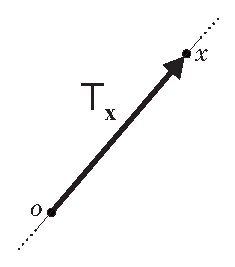
\includegraphics{partes/parte1/figs/c_geoafim/translacao.eps}
\titfigura{Representa��o da transla��o
$\tpv{\vto{x}}$.}\label{fg:translacao}
\end{figure}

A representa��o na figura � propositalmente tendenciosa quando
utiliza um segmento de linha retil�nea com ponta em seta indicando
o \emph{sentido} do mapeamento. Na verdade, qualquer elemento
figurativo, retil�neo ou n�o, que descrevesse este sentido poderia
ser utilizado. Como, tradicionalmente, retas s�o desenhadas como
linhas retil�neas infinitas, a representa��o de $\tpv{\vto{x}}$ na
figura tamb�m mostra uma \emph{dire��o} pois os pontos $\ele{o}$ e
$\ele{x}$ pertencem � reta $\saf{X}{X}{o}{F}$, onde
$\con{X}=sp\lch\vto{x}\rch$. Por isso, � poss�vel suprimir da
figura \ref{fg:translacao} o desenho desta reta.

Considerando uma segunda transla��o $\tpv{\vto{y}}$ que mapeia
$\ele{o}$ para um terceiro ponto $\ele{y}$ n�o pertencente � reta
$\saf{X}{X}{o}{F}$, tem-se a nova reta $\saf{Y}{Y}{o}{F}$, onde
$\con{Y}=sp\lch\vto{y}\rch$. Como se
tratam de duas retas distintas, pode-se dizer ent�o que um
\begin{figure}[!ht]
\centering
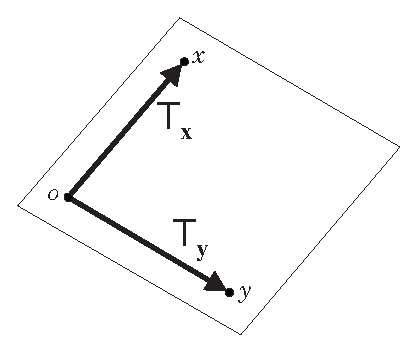
\includegraphics{partes/parte1/figs/c_geoafim/translacaoPlano}
\titfigura{Representa��o do plano $\saf{P}{P}{o}{F}$, onde
$\con{P}=sp\lch \vto{x},\vto{y}\rch$.}\label{fg:translacaoPlano}
\end{figure}
eventual conjunto $\lch \vto{x},\vto{y}\rch$ � linearmente
independente. Desta forma, o subespa�o afim $\saf{P}{P}{o}{F}$,
onde $\con{P}=sp\lch \vto{x},\vto{y}\rch$, � um plano,
tradicionalmente representado como na figura
\ref{fg:translacaoPlano}. O desenho do plano tamb�m pode ser
suprimido devido � representa��o das duas transla��es
$\tpv{\vto{x}}$ e $\tpv{\vto{y}}$ atuando no ponto $o$.

Ao se considerar um quarto ponto $\ele{z}$ n�o pertencente ao
plano $\saf{P}{P}{o}{F}$, resultado da atua��o  de uma transla��o
$\tpv{\vto{z}}$ no ponto $o$, tem-se uma terceira reta
$\saf{Z}{Z}{o}{F}$, onde $\con{Z}=sp\lch\vto{z}\rch$. De maneira
similar aos casos anteriores, na figura \ref{fg:translacaoTrid}
\begin{figure}[!ht]
\centering
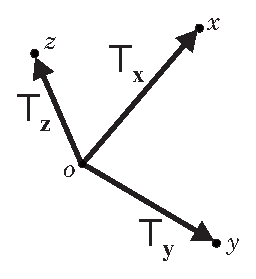
\includegraphics{partes/parte1/figs/c_geoafim/translacaoTrid}
\titfigura{Representa��o do subespa�o $\saf{K}{H}{o}{F}$, onde
$\con{K}=sp\lch
\vto{x},\vto{y},\vto{z}\rch$.}\label{fg:translacaoTrid}
\end{figure}
as representa��es das tr�s transla��es $\tpv{\vto{x}}$,
$\tpv{\vto{y}}$ e $\tpv{\vto{z}}$ atuando no mesmo ponto $o$
indicam um subespa�o afim tridimensional $\saf{H}{H}{o}{F}$, onde
$\con{H}=sp\lch \vto{x},\vto{y},\vto{z}\rch$.

\paragraph{Transla��es Compostas.}\index{transla��o!composta}
Seja o ponto $\ele{a}_1$ do espa�o puntual $\epo{A}$ e os vetores
$\vto{v}_1$, $\vto{v}_2$. A partir dos pontos
$\ele{a}_2:=\fua{\tpv{\vto{v}_1}}{\ele{a}_1}$ e
$\ele{a}_3:=\fua{\tpv{\vto{v}_2}}{\ele{a}_2}$, fica evidente que
$\fua{\tpv{\vto{v}_2+\vto{v}_1}}{\ele{a}_1}=\ele{a}_3$. Tais
pontos e transla��es est�o representados na figura
\ref{fg:translacaoComposicao}.
\begin{figure}[!ht] \centering
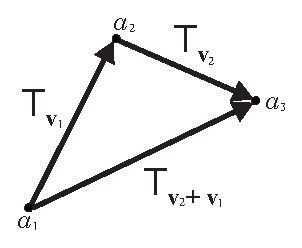
\includegraphics{partes/parte1/figs/c_geoafim/translacaoComposicao}
\titfigura{Representa��o da transla��o
$\tpv{\vto{v}_2+\vto{v}_1}$.}\label{fg:translacaoComposicao}
\end{figure}
J� foi demonstrado que a transla��o $\tpv{\vto{v}_2+\vto{v}_1}$ �
o resultado da composi��o $\tpv{\vto{v}_2}\circ\tpv{\vto{v}_1}$.
Como a composi��o de transla��es � comutativa, a atua��o de
$\tpv{\vto{v}_2}$ seguida por $\tpv{\vto{v}_1}$, ou seja
$\tpv{\vto{v}_1}\circ\tpv{\vto{v}_2}$, tamb�m deve definir a
representa��o de $\tpv{\vto{v}_2+\vto{v}_1}$.

\subsection{Paralelismo}\index{paralelismo}
Sejam o espa�o afim $\eaf{V}{A}{F}$ com dimens�o $n\geqslant2$ e
dois de seus subespa�os $\saf{U}{S}{a}{F}$ e $\saf{W}{S}{b}{F}$.
Diz-se que estes subespa�os s�o paralelos, ou seja
$\saf{U}{S}{a}{F}
\parallel \saf{W}{S}{b}{F}$, se
$\con{U}\subseteq\con{W}$ ou $\con{W}\subseteq\con{U}$. Tem-se, ent�o, as seguintes propriedades:
\begin{itemize}
   \item[i.] $\dim{\lpa\saf{U}{S}{a}{F}\rpa}=\dim{\lpa\saf{W}{S}{b}{F}\rpa}\implies\con{U}=\con{W}$;
   \item[ii.] $\ele{a}\in\epo{S}_\ele{b}$ ou $\ele{b}\in\epo{S}_\ele{a}$ $\implies\epo{S}_\ele{a}\subseteq\epo{S}_\ele{b}$ ou $\epo{S}_\ele{b}\subseteq\epo{S}_\ele{a}$;
   \item[iii.] $\ele{a}\notin\epo{S}_\ele{b}$ ou $\ele{b}\notin\epo{S}_\ele{a}$ $\implies\epo{S}_\ele{a}\cap\epo{S}_\ele{b}=\emptyset$.
\end{itemize}
\begin{prova}
\begin{itemize}
    \item[i.] Se $\dim{\lpa\saf{U}{S}{a}{F}\rpa}=\dim{\lpa\saf{W}{S}{b}{F}\rpa}$ ent�o $\dms{U}{F}=\dms{W}{F}$.
    Como $\con{U}\subseteq \con{W}$ ou $\con{W}\subseteq \con{U}$, ent�o $\con{U}=\con{W}$ ;
    \item[ii.] Seja $\lch\vto{v}_1,\cdots,\vto{v}_n\rch$ uma base de $\con{U}$ e $\lch\vto{v}_1,\cdots,\vto{v}_m\rch$ uma base de $\con{W}$, onde $\con{U}\subseteq\con{W}$. Se o ponto $\ele{x}\in\epo{S}_\ele{a}$, ent�o $\ele{x} = \sum_{i=1}^{n}\alpha_i\vto{v}_i\oplus\ele{a}$. Como $\ele{a}=\sum_{i=1}^{m}\beta_i\vto{v}_i\oplus\ele{b}$, ent�o
\begin{equation}
 \ele{x} = \sum_{i=1}^{m}\theta_i\vto{v}_i\oplus\ele{b}\,\nonumber
\end{equation}
onde $\theta_i=\alpha_i+\beta_i$, para $1\leqslant i\leqslant n$,  e  $\theta_i=\beta_i$, para $n < i\leqslant m$.
    \item[iii.] Considerando as condi��es da demonstra��o do �tem ii., seja $\ele{a}\notin\epo{S}_\ele{b}$. Tem-se ent�o que $\ele{a}=\vto{k}\oplus\ele{b}$, onde $\vto{k}\notin{W}$. Logo, $\ele{x} = \sum_{i=1}^{n}\lpa\alpha_i\vto{v}_i+\vto{k}\rpa\oplus\ele{b}$. Vamos admitir, por hip�tese, que o ponto $\ele{x}$ tamb�m perten�a a $\epo{S}_\ele{b}$. Para tal, deve-se ter obrigatoriamente $\alpha_i\vto{v}_i+\vto{k}=\theta_i\vto{v}_i$; o que � inconsistente com $\vto{k}\notin\con{W}$.
\end{itemize}
\end{prova}

\begin{figure}[!ht]
\centering
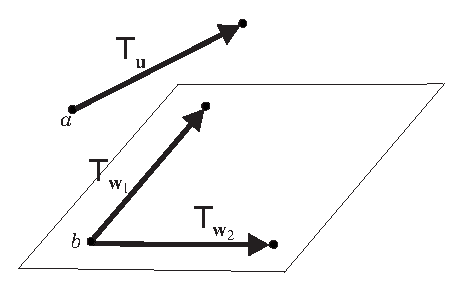
\includegraphics{partes/parte1/figs/c_geoafim/paralelismoRetaPlano}
\titfigura{Paralelismo onde o plano n�o cont�m a
reta.}\label{fg:paralelismoRetaPlano}
\end{figure}


\subsubsection{Representa��es} Considerando os subespa�os paralelos
$\saf{U}{S}{a}{F}$ uma linha e $\saf{W}{S}{b}{F}$ um plano, sejam
os pares $( \ele{a}, \lch\vto{u} \rch )$ e $( \ele{b},
\lch\vto{w}_1,\vto{w}_2 \rch )$ seus respectivos sistemas de
coordenadas. Admitindo a condi��o da propriedade iii, pode-se
observar o paralelismo entre uma reta e um plano na
figura \ref{fg:paralelismoRetaPlano}.

Agora, admitindo a condi��o da propriedade ii, tem-se a figura
\ref{fg:paralelismoRetaNoPlano}. Notar que os planos foram desenhados para dar maior clareza �s
representa��es.
\begin{figure}[!ht]
\centering
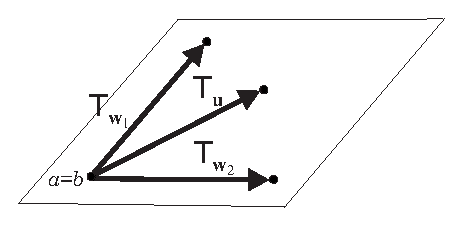
\includegraphics{partes/parte1/figs/c_geoafim/paralelismoRetaNoPlano}
\titfigura{Paralelismo onde a reta � subespa�o do
plano.}\label{fg:paralelismoRetaNoPlano}
\end{figure}

\begin{prp}[Quinto Postulado de Euclides]\index{Euclides!quinto postulado de}\rodape{Sobre este postulado,
\aut{Snapper e Troyer}\cite{snapper_1971_1}, p. 29, dizem o seguinte:``\textsl{[...]
Observe que o Quinto Postulado de Euclides pertence � geometria afim antes da geometria
Euclidiana. Geometria Euclidiana � uma geometria afim[...] sobre a qual  um arcabou�o
m�trico muito especial foi constru�do. Este arcabou�o m�trico n�o afeta a estrutura afim
[do espa�o puntual considerado...] O mesmo � v�lido para todos os outros espa�os
[puntuais] m�tricos[...] O �nico modo de se destruir o Quinto Postulado de Euclides �
considerar um espa�o que n�o � afim, como, por exemplo, um espa�o projetivo. }''.} Sejam
um subespa�o $m$-di\-men\-sio\-nal $\saf{U}{S}{a}{F}$  de um espa�o afim $\eaf{V}{A}{F}$
$n$-dimensional, $n\geqslant 2$, e um ponto qualquer $\ele{x}\in\epo{A}$, tal que
$\ele{x}\notin\epo{S}_\ele{a}$. Existe ent�o um e somente um subespa�o
$m$-di\-men\-sio\-nal $\saf{W}{S}{b}{F}$  de $\eaf{V}{A}{F}$, paralelo a
$\saf{U}{S}{a}{F}$, onde $\ele{x}\in\epo{S}_\ele{b}$.
\end{prp}
\begin{prova}
Para demonstrar exist�ncia, se $\con{W}=sp\lch\vto{u}\rch$, onde
$\vto{u}\in\con{U}$, e $\epo{S}_\ele{b}:=\lch \vto{w}\oplus\ele{b}
: \vto{w}\in\con{W}\rch$, ent�o tem-se uma reta $\saf{W}{S}{b}{F}$
paralela a $\saf{U}{S}{a}{F}$. A fim de demonstrar unicidade,
tem-se o seguinte: como $\saf{U}{S}{a}{F}$ e $\saf{W}{S}{b}{F}$
s�o paralelos de mesma dimens�o, tem-se que $\con{W}=\con{U}$.
Considerando, por hip�tese, um terceiro subespa�o $m$-dimensional
$\saf{U}{S}{c}{F}
\parallel \saf{U}{S}{a}{F}$ contento o ponto $\ele{x}$, tem-se
obrigatoriamente $\saf{U}{S}{c}{F} \parallel \saf{U}{S}{b}{F}$.
Com base nas propriedades do paralelismo, caso $\ele{c}=\ele{b}$,
tem-se que $\epo{S}_\ele{c}=\epo{S}_\ele{b}$. Se
$\ele{c}\neq\ele{b}$, obt�m-se a inconsist�ncia
$\epo{S}_\ele{b}\cap\epo{S}_\ele{c}=\emptyset$ j� que, por
hip�tese, $\ele{x}$ pertence simultaneamente aos espa�os
$\epo{S}_\ele{b}$ e $\epo{S}_\ele{c}$.
\end{prova}

\paragraph{Afinidades e Retas Paralelas.} Sejam o espa�o afim $\eaf{V}{A}{F}$ com dimens�o
$n\geqslant2$ e duas de suas retas paralelas quaisquer $\saf{U}{S}{a}{F}$ e
$\saf{U}{S}{b}{F}$, onde $\con{U}=sp\{\vto{v}\}$. Considerando uma transforma��o afim
$\map{\mathsf{A}}{\epo{A}}{\epo{A}}$ e um escalar qualquer $\con{\alpha}\in\con{F}$,
tem-se os pontos
$\fua{\mathsf{A}}{\alpha\vto{v}\oplus\ele{a}}=\alpha\fua{\vtf{l}}{\vto{v}}\oplus\fua{\mathsf{A}}{\ele{a}}$
e
$\fua{\mathsf{A}}{\alpha\vto{v}\oplus\ele{b}}=\alpha\fua{\vtf{l}}{\vto{v}}\oplus\fua{\mathsf{A}}{\ele{b}}$.
Com base nestas duas igualdades, pode-se concluir que a a��o de $\mathsf{A}$ nas retas
$\saf{U}{S}{a}{F}$ e $\saf{U}{S}{b}{F}$ gera as retas paralelas
$\saf{W}{S}{\fua{\mathsf{A}}{\ele{a}}}{F}$ e $\saf{W}{S}{\fua{\mathsf{A}}{\ele{b}}}{F}$,
onde $\con{W}=sp\{\fua{\vtf{l}}{\vto{v}}\}$. Desta forma, costuma-se dizer que uma
afinidade preserva o paralelismo, conforme mostrado na figura \ref{fg:afinidade}.
\begin{figure}[!ht]
\centering
\begin{center}
\input{partes/parte1/figs/c_geoafim/afinidade.pstex_t}
\end{center}
\titfigura{A atua��o da afinidade $\mathsf{L}$.}\label{fg:afinidade}
\end{figure}



\subsection{Dila��o}\index{dila��o}
Seja um espa�o afim $\eaf{V}{A}{F}$ de dimens�o $n\geqslant 1$, o conjunto
$\{\vto{u}_1,\cdots,\vto{u}_n\}$ uma base qualquer de $\evt{V}{\con{F}}$. Diz-se que a
afinidade no mapeamento $\map{\mathsf{D}}{\epo{A}}{\epo{A}}$ � uma dila��o\rodape{Alguns
autores adotam o termo ``dilata��o'' no lugar de dila��o. Este livro entende dila��o
conforme \aut{Houaiss e Villar}\cite{houaiss_2001_1} que, dentre outros significados,
apresenta o termo como o ``ato ou efeito de expandir-se, ampliar-se''.} de $\epo{A}$ se
\begin{equation}\label{eq:dilacao}
\fua{\mathsf{D}}{\vto{v}\oplus\ele{a}}=\fua{\vtf{s}}{\vto{v}}
\oplus\fua{\mathsf{D}}{\ele{a}}\,,\,\forall\, \ele{a}\in\epo{A},\vto{v}\in\con{V}\,,
\end{equation}
onde operador $\vtf{s}\in\cfl{V}{V}$,  chamado \emph{estiramento}\index{estiramento}, � sim�trico e positivo-definido.
O estiramento $\vtf{s}$ � representante de um tensor de afinidade sim�trico positivo-definido
$\tnr{S}\in\cft{\con{V}^2}{\con{F}}$, chamado \emph{tensor de estiramento}\index{tensor!de estiramento}.   Considerando $\con{T}^{\otimes}_{\con{V}^2}$ uma base de $\ete{\con{V}^2}{\con{F}}$, gerada pelos  tensores di�dicos
${\vto{u}_{i_1}}\otimes{\vto{u}_{i_2}}$, onde $i_j=1,\cdots,n$ e $\vto{u}_{i_j}$ s�o os
autovetores\rodape{Ver se��o \ref{sec:espectro} e o Teorema \ref{teo:BasesPoliadicas}.}
de $\tnr{S}$, � poss�vel escrever
\begin{equation}
\tnr{S}=\sum_{i=1}^n\fua{\vtf{f}_{ii}^{\con{T}^{\otimes}_{\con{V}^2}}}{\tnr{S}}{\vto{u}_{i}}\otimes{\vto{u}_{i}}.
\end{equation}
Os escalares positivos
$\alpha_{ii}:=\fua{\vtf{f}_{ii}^{\con{T}^{\otimes}_{\con{V}^2}}}{\tnr{S}}$ s�o os
autovalores de $\tnr{S}$, denominados \emph{coeficientes de
estiramento}\index{coeficiente!de estiramento}. Um coeficiente $\alpha_{ii}$ pode
ser classificado como uma \emph{contra��o}\index{contra��o}, se $\alpha_{ii}<1$, ou como
uma \emph{expans�o}\index{expans�o}, se $\alpha_{ii}>1$. No caso de \emph{estiramento
proporcional}\index{estiramento!proporcional}, ou seja $\alpha_{11}=\cdots=\alpha_{nn}$, tais
classifica��es s�o aplic�veis ao tensor de estiramento como um todo.

Pode-se demonstrar facilmente que as dila��es, em rela��o � composi��o, possuem as
propriedades de
\begin{itemize}
    \item[i.] Associatividade:
$\mathsf{D}_1\circ\lpa\mathsf{D}_2\circ\mathsf{D}_3\rpa=
\lpa\mathsf{D}_1\circ\mathsf{D}_2\rpa\circ\mathsf{D}_3$;
    \item[ii.] Elemento Identidade: $\mathsf{D}_1\circ\mathsf{D}_2=\mathsf{D}_2$ se $\mathsf{D}_1=\fun{i}_{\epo{A}}$;
    \item[iii.] Elemento Inverso: $\mathsf{D}_1\circ\mathsf{D}_1^{-1}=\fun{i}_{\epo{A}}$.
\end{itemize}
As propriedades ii e iii baseiam-se no fato de que a fun��o identidade
$\fun{i}_{\epo{A}}$ tamb�m � uma dila��o (com coeficientes unit�rios) e que $\det
\tnr{S}\neq 0$. Desta forma, o conjunto $\con{D}$ de todas as dila��es de $\epo{A}$
define o grupo $\grp{D}$.


Agora, considerando uma transla��o qualquer $\tpv{\vto{w}}$,
pode-se realizar o seguinte desenvolvimento:
\begin{equation}
\fua{\tpv{\vto{w}}}{\vto{v}\oplus\ele{a}}=\vto{w}\oplus\lpa\vto{v}\oplus\ele{a}\rpa
=\vto{v}\oplus\lpa\vto{w}\oplus\ele{a}\rpa
=\vto{v}\oplus\fua{\tpv{\vto{w}}}{\ele{a}},
\end{equation}
de onde se pode afirmar, comparando com a igualdade (\ref{eq:dilacao}), que
$\tpv{\vto{w}}$ � uma dila��o de coeficientes unit�rios. No entanto, nem toda dila��o �
uma transla��o j� que � poss�vel ocorrer simultaneamente
$\fua{\mathsf{D}}{\ele{a}}=\ele{a}$ e
$\fua{\mathsf{D}}{\vto{v}\oplus\ele{a}}\neq\vto{v}\oplus\ele{a}$, fato que � imposs�vel
no caso de transla��es: se $\fua{\tpv{}}{\ele{a}}=\ele{a}$ ent�o obrigatoriamente
$\fua{\tpv{}}{\vto{v}\oplus\ele{a}}=\vto{v}\oplus\ele{a}$.

\subsubsection{Dila��o Centrada}\index{dila��o!central} A dila��o que n�o � uma transla��o �
dita dila��o centrada, representada por $\dcl{a}$, onde o ponto $\ele{a}$ � considerado o
\emph{centro da dila��o}\index{centro!da dila��o}. Desta forma,
\begin{equation}
\fua{\dcl{a}}{\vto{v}\oplus\ele{a}}=\fua{\vtf{s}}{\vto{v}}\oplus\ele{a}\,,\,\forall\,
\ele{a}\in\epo{A},\vto{v}\in\con{V}\,.
\end{equation}

\subsubsection{Representa��es} Tomando o ponto $\ele{a}$ e o
subconjunto $\con{U}=sp\lch \vto{v} \rch$, pode-se definir a reta $\saf{U}{S}{a}{F}$.
Considerando a dila��o $\mathsf{D}_1$, obt�m-se, da mesma forma, que
$\fua{\mathsf{D}_1}{a}$ e $\fua{\vtf{s}}{\vto{v}}$ definem a reta
$\saf{U}{S}{\fua{\mathsf{D}_1}{a}}{F}$. Considerando que a dila��o n�o � centrada, ou
seja $\ele{a}\neq\fua{\mathsf{D}_1}{a}$, as retas em quest�o s�o representadas segundo a
figura \ref{fg:dilacao}.

\begin{figure}[!ht]
\centering
\begin{center}
\input{partes/parte1/figs/c_geoafim/dilacao.pstex_t}
\end{center}
\titfigura{A dila��o n�o centrada $\mathsf{D}_1$.}\label{fg:dilacao}
\end{figure}
Esta figura mostra uma importante caracter�stica representativa das transla��es: como os
valores das coordenadas de $\fua{\vtf{s}}{\vto{v}}$ s�o m�ltiplos das coordenadas de
$\vto{v}$ na base de autovetores de $\vtf{s}$, o tamanho das linhas retil�neas
$\overline{\ele{a},\vto{v}\oplus\ele{a}}$ e
$\overline{\fua{\mathsf{D}_1}{a},\fua{\mathsf{D}_1}{\vto{v}\oplus\ele{a}}}$ refletem esta
multiplicidade. Em outras palavras, al�m de evidenciar aspectos envolvendo dire��o e
sentido, conv�m que a representa��o de uma transla��o tamb�m informe aspectos
relacionados a \emph{magnitude}\footnote{Uma das formas para mensurar esta magnitude
utiliza o conceito de m�trica.}. A figura \ref{fg:dilacaoCentral} mostra a dila��o
centrada $\mathsf{D}_2$ definida por $\vtf{s}$.
\begin{figure}[!ht]
\centering
\begin{center}
\input{partes/parte1/figs/c_geoafim/dilacent.pstex_t}
\end{center}
\titfigura{A dila��o $\mathsf{D}_2$ com centro em
$\ele{a}$.}\label{fg:dilacaoCentral}
\end{figure}


\begin{prp}
Sejam um espa�o afim $\eaf{V}{A}{F}$ e uma dila��o $\mathsf{D}$ de $\epo{A}$ com
coeficientes $\alpha_{ii}$. Considerando em $\epo{A}$ um ponto ``$\ele{a}$'' qualquer, as
dila��es centrais  $\dcl{a}$, $\dcl{\fua{\mathsf{D}}{\ele{a}}}$ com coeficientes
$\alpha_{ii}$ e a transla��o $\tpv{\vto{u}}$, onde
$\fua{\mathsf{D}}{\ele{a}}=\fua{\tpv{\vto{u}}}{\ele{a}}$, � sempre poss�vel realizar as
seguintes decomposi��es:
\begin{equation}
\mathsf{D} = \tpv{\vto{u}}\circ\dcl{a} =
\dcl{\fua{\mathsf{D}}{\ele{a}}}\circ\tpv{\vto{u}}\,,\nonumber
\end{equation}
onde cada uma delas � �nica.
\end{prp}
\begin{prova}
A unicidade das decomposi��es � diretamente verificada j� que as
fun��es $\tpv{\vto{u}}$, $\dcl{a}$ e
$\dcl{\fua{\mathsf{D}}{\ele{a}}}$ s�o �nicas. Dado um vetor
$\vto{v}$ e considerando a defini��o de dila��o, � poss�vel
realizar os seguintes desenvolvimentos:
\begin{eqnarray}
\fua{\mathsf{D}}{\vto{v}\oplus\ele{a}}&=&\fua{\vtf{s}}{\vto{v}}\oplus\fua{\mathsf{D}}{\ele{a}}
\nonumber\\
&=&\fua{\vtf{s}}{\vto{v}}\oplus\vto{u}\oplus\ele{a}
\nonumber\\
&=&\vto{u}\oplus\fua{\vtf{s}}{\vto{v}}\oplus\ele{a}
\nonumber\\
&=&\fua{\tpv{\vto{u}}\circ\dcl{a}}{\vto{v}\oplus\ele{a}}\nonumber
\end{eqnarray}
e
\begin{eqnarray}
\fua{\mathsf{D}}{\vto{v}\oplus\ele{a}}&=&\fua{\vtf{s}}{\vto{v}}\oplus\fua{\mathsf{D}}{\ele{a}}
\nonumber\\
&=&-\vto{v}\oplus\fua{\vtf{s}}{\vto{v}}\oplus\vto{v}\oplus\fua{\mathsf{D}}{\ele{a}}
\nonumber\\
&=&-\vto{v}\oplus\fua{\vtf{s}}{\vto{v}}\oplus\vto{v}\oplus\fua{\tpv{\vto{u}}}{\ele{a}}
\nonumber\\
&=&\fua{\dcl{\fua{\mathsf{D}}{\ele{a}}}}{\vto{v}\oplus\fua{\tpv{\vto{u}}}{\ele{a}}}
\nonumber\\
&=&\fua{\dcl{\fua{\mathsf{D}}{\ele{a}}}\circ\tpv{\vto{u}}}{\vto{v}\oplus\ele{a}}\,.\nonumber
\end{eqnarray}
\end{prova}

\section{Espa�os Afins M�tricos}

\subsection{Espa�o Afim M�trico}\index{espa�o!afim!m�trico}\label{sec:AfimMetrico}
Seja $\saf{U}{S}{\ele{a}}{F}$ subespa�o afim qualquer de
$\eaf{V}{A}{F}$, tal que o espa�o vetorial $\evt{U}{F}$ � m�trico.
Dado um sistema de coordenadas $(\ele{o} , \tilde{\con{U}})$ do
subespa�o afim em quest�o, se o espa�o puntual $\epo{S}_\ele{a}$
for m�trico devido � igualdade
\begin{equation}\label{eq:distanciaPontos}
\fua{d}{\vto{v}_1\oplus\ele{o},\vto{v}_2\oplus\ele{o}}=\fua{\varrho}{\vto{v}_1,\vto{v}_2}
\,,\,\forall\,\vto{v}_1,\vto{v}_2\in\con{U}\,,
\end{equation}
diz-se ent�o que espa�o afim $\eaf{V}{A}{F}$ � m�trico. Seguindo o
mesmo padr�o desta defini��o, os diversos tipos de espa�os
vetoriais m�tricos qualificam com a mesma nomenclatura seus
respectivos espa�os puntual e afim relacionados. Um \emph{espa�o
afim de Banach}\index{Banach!espa�o afim de} � definido por um
espa�o de Banach se, em seu espa�o puntual,
\begin{equation}
\|{\vto{v}_1\oplus\ele{o}}\|:=\|\vto{v}_1\|\,,\,\forall\,\vto{v}_1\in\con{U}\,.
\end{equation}
De maneira similar, um espa�o de Hilbert define um \emph{espa�o
afim de Hilbert}\index{Hilbert!espa�o afim de} caso seu espa�o
puntual for de Hilbert segundo
\begin{equation}
\lpa\vto{v}_1\oplus\ele{o}\rpa\cdot\lpa\vto{v}_2\oplus\ele{o}\rpa:=\vto{v}_1\cdot\vto{v}_2\,,\,\forall\,\vto{v}_1,\vto{v}_2\in\con{U}\,.
\end{equation}

\subsection{Afinidades Isom�tricas}\index{afinidade!isom�trica}\label{sec:afinidadeIsometrica}

Seja $\eaf{V}{A}{F}$ um espa�o afim  m�trico e um espa�o vetorial $\evl{V}{V}{F}$. Uma
afinidade $\mathsf{K}$ de $\epo{A}$ � dita isom�trica se o operador linear
$\vtf{k}\in\cfl{V}{V}$ em
\begin{equation}\label{eq:afinidadeIsometrica}
\fua{\mathsf{K}}{\vto{v}\oplus\ele{a}}=\fua{\vtf{k}}{\vto{v}}\oplus\fua{\mathsf{K}}{\ele{a}},\,\forall
\ele{a}\in\epo{A},\vto{v}\in\con{V},
\end{equation}
for uma isometria. Em particular, se
$\fua{\mathsf{K}}{\ele{a}}=\ele{a}$, diz-se que a afinidade
isom�trica, com representa��o $\mathsf{K}_\ele{a}$, est� centrada
em $\ele{a}$. Neste caso,
\begin{itemize}
\item[i.] se $\det\vtf{k}=+1$, $\mathsf{K}$ � uma
\emph{rota��o}\index{rota��o} e $\mathsf{K}_\ele{a}$ uma rota��o centrada em $\ele{a}$;
    \item[ii.] se $\det\vtf{k}=-1$, $\mathsf{K}$ � uma \emph{reflex�o}\index{reflex�o} e $\mathsf{K}_\ele{a}$ uma reflex�o centrada em $\ele{a}$.
\end{itemize}
Para o caso de $\det\vtf{k}=1$, diz-se que o operador linear $\vtf{k}$ representa o tensor de afinidade $\tnr{R}\in\cft{\con{V}^2}{\con{F}}$, chamado \emph{tensor de rota��o}\index{tensor!de rota��o}. Nas reflex�es, por sua vez, $\vtf{k}$ representa o \emph{tensor de reflex�o}\index{tensor!de reflex�o} $\overline{\tnr{R}}\in\cft{\con{V}^2}{\con{F}}$.

\subsubsection{Representa��es} Sejam os sistema de coordenadas $(
\ele{o},\con{U})$ do espa�o afim $n$-dimensional $\eaf{V}{A}{F}$,
onde $\con{U}=\lch \vto{u}_1,\cdots,\vto{u}_n \rch$. Dado um plano
$\saf{V_{pq}}{S}{o}{F}$, onde o subconjunto $\con{V}_{pq}=sp\lch
\vto{u}_p ,\vto{u}_q \rch$, seja $\theta_{pq}$ o menor �ngulo
definido entre as linhas
$\overline{\ele{o},\vto{u}_p\oplus\ele{o}}$ e
$\overline{\ele{o},\vto{u}_q\oplus\ele{o}}$. Desta forma, �
evidente que $0<\theta_{pq}<\pi$.

Considerando um espa�o vetorial $\evl{V}{V}{F}$, seja um operador
linear $\vtf{l}\in\cfl{V}{V}$. Aplicando este operador nos vetores
da base $\con{U}$, os �ngulos $\theta_{pq}$ se modificam para
$\tilde{\theta}_{pq}$ na base $\con{\tilde{U}}=\lch
\fua{\vtf{l}}{\vto{u}_1},\cdots,\fua{\vtf{l}}{\vto{u}_n} \rch$.
Diz-se que $\vtf{l}$ \emph{preserva orienta��o} se
$0<\tilde{\theta}_{pq}<\pi$ for v�lido para qualquer �ngulo
$\tilde{\theta}_{pq}$. Neste caso, pode-se obter que $\det\vtf{l}
> 0$. Se pelo menos um dos �ngulos $\tilde{\theta}_{pq}$ n�o
obedecer a desigualdade anterior, obt�m-se que $\det\vtf{l} < 0$.

Considerando, agora, que $\eaf{V}{A}{F}$ � bidimensional, seja uma
afinidade isom�trica centrada cuja regra �
\begin{equation}
\fua{\mathsf{K}_{\ele{x}}}{\vto{v}\oplus\ele{x}}=\fua{\vtf{k}}{\vto{v}}\oplus\ele{x},
\end{equation}
onde $\ele{x}\in\epo{A}$, $\vtf{k}\in\cfl{V}{V}$ e
$\vto{v}\in\con{V}$. Se $\vtf{k}$ preservar orienta��o, ent�o
tem-se na figura \ref{fg:rotacao} a representa��o de rota��es
centradas.
\begin{figure}[!ht]
\centering
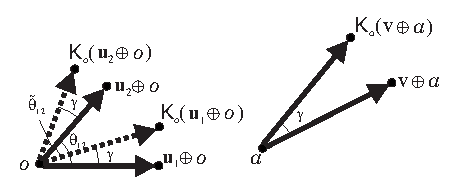
\includegraphics{partes/parte1/figs/c_geoafim/rotacao}
\titfigura{Rota��es centradas.}\label{fg:rotacao}
\end{figure}

Caso $\vtf{k}$ n�o preserve orienta��o realizando sobre
$\vto{u}_2$ o efeito combinado de uma rota��o com uma mudan�a de
sinal de suas coordenadas, por exemplo, tem-se as reflex�es
conforme a figura \ref{fg:reflexao}.
\begin{figure}[!ht]
\centering
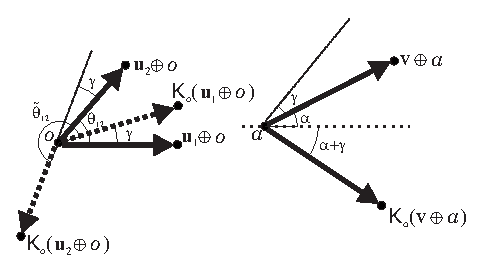
\includegraphics{partes/parte1/figs/c_geoafim/reflexao}
\titfigura{Reflex�es centradas.}\label{fg:reflexao}
\end{figure}
Embora n�o esteja representado, uma reflex�o tamb�m pode realizar este efeito combinado em ambos os vetores $\vto{u}_1$ e $\vto{u}_2$.


\begin{prp}\label{prop:AfinidadesIgualdade}
Seja um espa�o afim $\eaf{V}{A}{F}$, uma afinidade isom�trica
centrada $\mathsf{K}_{\ele{a}}$ e $\mathsf{D}$ uma dila��o
qualquer de $\epo{A}$. � sempre v�lido que a afinidade
\begin{equation}
\mathsf{D}\circ\mathsf{K}_{\ele{a}}=\mathsf{K}_{\fua{\mathsf{D}}{\ele{a}}}\circ\mathsf{D}\,.\nonumber
\end{equation}
\end{prp}
\begin{prova}
Considerando $\mathsf{D}$ de coeficiente $\ele{r}$, um vetor
qualquer $\vto{v}\in\con{V}$ e um ponto qualquer
$\ele{a}\in\epo{A}$, podemos realizar o seguinte desenvolvimento:
\begin{eqnarray}
\fua{\mathsf{D}\circ\mathsf{K}_{\ele{a}}}{\vto{v}\oplus\ele{a}}&=&\fua{\mathsf{D}}{\fua{\vtf{k}}{\vto{v}}\oplus\ele{a}}\nonumber\\
&=&\fua{\vtf{k}}{\ele{r}\vto{v}}\oplus\fua{\mathsf{D}}{\ele{a}}\nonumber\\
&=&\fua{\mathsf{K}_{\fua{\mathsf{D}}{\ele{a}}}}{\ele{r}\vto{v}\oplus\fua{\mathsf{D}}{\ele{a}}}\nonumber\\
&=&\fua{\mathsf{K}_{\fua{\mathsf{D}}{\ele{a}}}\circ\mathsf{D}}{\vto{v}\oplus\ele{a}}\,.\nonumber
\end{eqnarray}
\end{prova}


\subsection{Perpendicularidade}\index{perpendicularidade}
Sejam o espa�o afim produto interno $\eaf{V}{A}{F}$ com dimens�o
$n\geqslant2$ e dois de seus subespa�os $\saf{U}{S}{a}{F}$ e
$\saf{W}{S}{b}{F}$. Diz-se que $\saf{U}{S}{a}{F}$ � perpendicular
a $\saf{W}{S}{b}{F}$, ou $\saf{U}{S}{a}{F}\perp\saf{W}{S}{b}{F}$,
se $\con{U}\perp\con{W}$.

\subsubsection{Representa��o} Seja $\eaf{V}{A}{\real}$ um espa�o afim de Hilbert com dimens�o
$n\geqslant2$, dois de seus subespa�os $\saf{U}{S}{a}{\real}$,
$\saf{W}{S}{a}{\real}$ e os vetores quaisquer $\vto{u}\in\con{U}$,
$\vto{w}\in\con{W}$. Considerando que os subespa�os n�o s�o
paralelos, a partir da desigualdade de Cauchy-Schwarz\rodape{ Ver se��o \ref{sec:EspacoHilbert}.}, � poss�vel
quantificar o valor do menor �ngulo $\theta$ formado pelas linhas
$\overline{\ele{a},\vto{u}\oplus\ele{a}}$ e
$\overline{\ele{a},\vto{w}\oplus\ele{a}}$ especificando que
\begin{equation}\label{eq:anguloProdInterno}
\cos\theta:=\frac{\vto{u}\cdot\vto{w}}{ \|\vto{u}\|
\|\vto{w}\|}\,,\, 0\leqslant\theta\leqslant\pi\,.
\end{equation}
Agora, seja $\saf{U}{S}{a}{\real}$ uma reta onde $\con{U}=sp\lch
\vto{u}_1 \rch$ e  $\saf{W}{S}{a}{\real}$ um plano cujo conjunto
$\con{W}=sp\lch \vto{w}_1,\vto{w}_2 \rch$. Se estes dois
subespa�os afins forem perpendiculares, pela defini��o anterior,
tem-se a representa��o da figura
\ref{fg:perpendicularidadeRetaPlano}.
\begin{figure}[!ht]
\centering
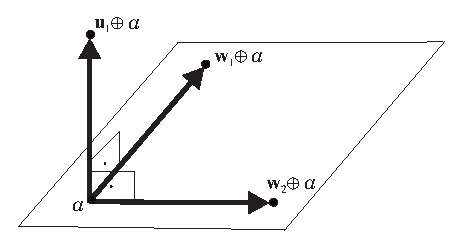
\includegraphics{partes/parte1/figs/c_geoafim/perpendicularidadeRetaPlano}
\titfigura{Perpendicularidade de uma reta com um
plano.}\label{fg:perpendicularidadeRetaPlano}
\end{figure}
Atrav�s da defini��o de perpendicularidade, a linha
$\overline{\ele{a},\vto{u}_1\oplus\ele{a}}$ forma um �ngulo de
valor $\pi/ 2$ com todas as linhas do tipo $\overline{\ele{a},\vto{w}\oplus\ele{a}}$. Diz-se ent�o que a reta
$\saf{U}{S}{a}{\real}$ ``encontra'' o plano $\saf{W}{S}{a}{\real}$
segundo um �ngulo reto. Procedimento id�ntico pode ser aplicado ao
caso de dois planos n�o paralelos.


\subsection{Vetores Axiais}\index{vetor!axial}
Sejam um espa�o afim $\eaf{V}{A}{F}$, um espa�o vetorial
$\evl{V}{V}{F}$ e uma reflex�o qualquer $\vtf{m}\in\cfl{V}{V}$. Um
vetor n�o nulo $\vto{r}\in\con{V}$ � dito axial se sempre existir pelo
menos uma rota��o $\vtf{r}\in\cfl{V}{V}$ tal que
\begin{equation}\label{eq:vetorAxial}
\fua{\vtf{m}}{\vto{r}}=\fua{\vtf{r}}{\vto{r}}.
\end{equation}
Pode-se concluir ent�o que vetores axiais s�o invariantes � mudan�a de sinal de suas coordenadas provocada pela reflex�o. Vetores que n�o obedecem (\ref{eq:vetorAxial}) s�o denominados
\emph{polares}\index{vetor!polar}.

Os vetores axiais s�o geralmente utilizados para representar
quantidades de natureza n�o vetorial, mas que, eventualmente,
precisam ser orientadas, como, por exemplo, �reas, volumes e
hiper-volumes. � comum construir vetores axiais a partir de
vetores polares utilizando o conceito de produto externo,
apresentado a seguir.


\subsection{Produto Externo}\index{produto!externo}
Seja o espa�o vetorial $\evt{V}{F}$ e o conjunto
$\con{P}\subseteq\con{V}$ formado por vetores axiais. Uma
transforma��o bin�ria
$\map{\barwedge}{\con{V}\times\con{V}}{\con{P}}$ � denominada
produto externo se os seguintes axiomas forem obedecidos:
\begin{itemize}
    \item[i.] $\vto{v}_1\barwedge\lpa\vto{v}_2+\vto{v}_3\rpa=\vto{v}_1\barwedge\vto{v}_2+\vto{v}_1\barwedge\vto{v}_3\,,\,\forall\vto{v}_1,\vto{v}_2,\vto{v}_3\in\con{V}$;
    \item[ii.] $\ele{a}_1\vto{v}_1\barwedge\ele{a}_2\vto{v}_2=\ele{a}_1\ele{a}_2\lpa \vto{v}_1\barwedge\vto{v}_2 \rpa\,,\,\forall\vto{v}_1,\vto{v}_2\in\con{V},\ele{a}_1,\ele{a}_2\in\con{F}$;
    \item[iii.] $\vto{v}_1\barwedge\vto{v}_2=-\lpa\vto{v}_2\barwedge\vto{v}_1\rpa\,,\,\forall\vto{v}_1,\vto{v}_2\in\con{V}$;
    \item[iv.] $\vto{v}_1\barwedge\vto{v}_2=\vto{0}$, se $\vto{v}_1,\vto{v}_2\in\con{V}$ forem linearmente dependentes.
\end{itemize}

\subsubsection{Produto Vetorial}\index{produto!vetorial}\label{sec:produtoVetorial} Seja o par ordenado $(\ehr{V}{\real},\hat{\tnr{P}})$
um espa�o orientado de Hilbert tridimensional. Um produto externo
$\map{\wedge}{\con{V}\times\con{V}}{\con{V}}$ � denominado produto vetorial se, para
quaisquer $\vto{v},\vto{w}\in\con{V}$,
\begin{equation}\label{eq:produtoVetorial}
\vto{v}\wedge\vto{w}=\hat{\tnr{P}}\odot_2\lpa\vto{v}\otimes\vto{w}\rpa\,.
\end{equation}
Desta defini��o, dado um vetor $\vto{u}\in\con{V}$ qualquer, o escalar
\begin{eqnarray}\label{eq:produtoInternoVetorial}
\vto{u}\cdot\lpa\vto{v}\wedge\vto{w}\rpa & = & \vto{u} \odot_1
\lco\hat{\tnr{P}}\odot_2\lpa\vto{v}\otimes\vto{w}\rpa\rco\nonumber\\
&= &\hat{\tnr{P}}\odot_3\lpa\vto{u}\otimes\vto{v}\otimes\vto{w}\rpa\,.
\end{eqnarray}
A partir desta igualdade, a anti-simetria de $\hat{\tnr{P}}$ promove
\begin{equation}\label{eq:produtoInternoVetorial1}
\vto{u}\cdot\lpa\vto{v}\wedge\vto{w}\rpa=\vto{v}\cdot\lpa\vto{w}\wedge\vto{u}\rpa=\vto{w}\cdot\lpa\vto{u}\wedge\vto{v}\rpa
\end{equation}
e
\begin{equation}
\vto{u}\cdot\lpa\vto{v}\wedge\vto{w}\rpa=-\vto{v}\cdot\lpa\vto{u}\wedge\vto{w}\rpa
=-\vto{u}\cdot\lpa\vto{w}\wedge\vto{v}\rpa=-\vto{w}\cdot\lpa\vto{v}\wedge\vto{u}\rpa\,.
\end{equation}

\noindent\begin{prova} Para que a defini��o (\ref{eq:produtoVetorial}) seja aceit�vel,
ela deve respeitar os axiomas apresentados na se��o anterior. Vamos ver se isto ocorre
para cada um deles nos itens respectivos a seguir, considerando
$\vto{v}_1,\vto{v}_2,\vto{v}_3\in\con{V}$ quaisquer.
\begin{itemize}
\item[i.] Seja o seguinte desenvolvimento:
\begin{eqnarray*}
\vto{v}_1\wedge\lpa\vto{v}_2+\vto{v}_3\rpa&=&
\hat{\tnr{P}}\odot_2\lpa\vto{v}_1\otimes\lpa\vto{v}_2+\vto{v}_3\rpa\rpa\\
&=&\hat{\tnr{P}}\odot_2\lpa\vto{v}_1\otimes\vto{v}_2+
\vto{v}_1\otimes\vto{v}_3\rpa\\
&=&\hat{\tnr{P}}\odot_2\lpa\vto{v}_1\otimes\vto{v}_2\rpa+\hat{\tnr{P}}\odot_2\lpa
\vto{v}_1\otimes\vto{v}_3\rpa\,.
\end{eqnarray*}
\item[ii.] Seja o seguinte desenvolvimento para $\ele{a}_1,\ele{a}_2\in\con{F}$:
\begin{eqnarray*}
\ele{a}_1\vto{v}_1\wedge\ele{a}_2\vto{v}_2&=&\hat{\tnr{P}}\odot_2\lpa \ele{a}_1\vto{v}_1 \otimes \ele{a}_2\vto{v}_2\rpa\\
&=&\ele{a}_1\ele{a}_2\hat{\tnr{P}}\odot_2\lpa \vto{v}_1 \otimes \vto{v}_2\rpa\,.
\end{eqnarray*}
\item[iii.] Tem-se o desenvolvimento:
\begin{eqnarray*}
\vto{v}_1\wedge\vto{v}_2&=&\hat{\tnr{P}}\odot_2\lpa \vto{v}_1\otimes\vto{v}_2 \rpa\\
&=&-\hat{\tnr{P}}_{(2,3)}\odot_2\lpa \vto{v}_1\otimes\vto{v}_2 \rpa\\
&=&-\hat{\tnr{P}}\odot_2\lpa \vto{v}_2\otimes\vto{v}_1 \rpa\,.
\end{eqnarray*}

\item[iv.] A demonstra��o do �tem iv. das propriedades apresentadas na se��o \ref{sec:HiperdeterminanteOperador} mostrou que um tensor anti-sim�trico com argumento formado por elementos linearmente dependentes resulta zero. Logo, seja um vetor n�o nulo $\vto{u}\in\con{V}$ e dois vetores $\vto{v}_1$ e $\vto{v}_2$ linearmente dependentes. Com base em (\ref{eq:produtoInternoVetorial}), tem-se
\begin{equation*}
\vto{u}\cdot\lpa\vto{v}_1\wedge\vto{v}_2\rpa=\hat{\tnr{P}}\odot_3\lpa\vto{u}\otimes\vto{v}_1\otimes\vto{v}_2\rpa=0\,.
\end{equation*}
J� que $\vto{u}$ � n�o nulo, ent�o obt�m-se o resultado do �tem.
\end{itemize}
\end{prova}

Agora, seja o subconjunto $\con{U}=\lch \vun{u}_1, \vun{u}_2, \vun{u}_3\rch$ de $\con{V}$
uma base ortonormal de $\ehr{V}{\real}$. Dados os vetores
quaisquer $\vto{v}$ e $\vto{w}$ de $\con{V}$, tem-se que
\begin{equation}\label{eq:coordPositivOrientado}
 \lpa \vto{v}\wedge\vto{w}\rpa_i = \sum_{j=1}^3 \sum_{k=1}^3 \epsilon_{ijk}\mav{v}{U}_{j}\mav{w}{U}_{k}
\end{equation}
para $\con{U}$ positivamente orientada e
\begin{equation}\label{eq:coordNegativOrientado}
 \lpa \vto{v}\wedge\vto{w}\rpa_i = \sum_{j=1}^3 \sum_{k=1}^3 -\epsilon_{ijk}\mav{v}{U}_{j}\mav{w}{U}_{k}
\end{equation}
quando tal base for negativamente orientada. Neste contexto, para $\con{U}$ positivamente orientada e utilizando a igualdade (\ref{eq:prodLeviCivita}), pode-se realizar o seguinte desenvolvimento
\begin{eqnarray}
\mav{\vto{u}\wedge\vto{v}\wedge\vto{w}}{U}_{i}&=& \sum_{j=1}^3 \sum_{k=1}^3 \epsilon_{ijk}\mav{u}{U}_{j}\mav{\vto{v}\wedge\vto{w}}{U}_{k}\nonumber\\
&=& \sum_{j=1}^3 \sum_{k=1}^3 \sum_{l=1}^3\sum_{m=1}^3\epsilon_{ijk}\epsilon_{klm}\mav{u}{U}_{j}\mav{v}{U}_{l}\mav{w}{U}_{m}\nonumber\\
&=& \sum_{j=1}^3 \sum_{k=1}^3 \sum_{l=1}^3\sum_{m=1}^3\lpa\delta_{il}\delta_{jm}-\delta_{im}\delta_{jl} \rpa\mav{u}{U}_{j}\mav{v}{U}_{l}\mav{w}{U}_{m}\nonumber\\
&=& \sum_{j=1}^3 \mav{u}{U}_{j}\mav{w}{U}_{j}\mav{v}{U}_{i}- \sum_{j=1}^3\mav{u}{U}_{j}\mav{v}{U}_{j}\mav{w}{U}_{i}\nonumber\\
&=& \lco\lpa\vto{u}\cdot\vto{w}\rpa\vto{v}\rco_i^{\con{U}}- \lco\lpa\vto{u}\cdot\vto{v}\rpa\vto{w}\rco_i^{\con{U}}\,.
\end{eqnarray}
Em termos gerais, pode-se concluir desta �ltima igualdade que
\begin{equation}\label{eq:produtoTriplo}
\vto{u}\wedge\vto{v}\wedge\vto{w} = \lpa\vto{u}\cdot\vto{w}\rpa\vto{v} - \lpa\vto{u}\cdot\vto{v}\rpa\vto{w}\,,\,\forall\,\vto{u},\vto{v},\vto{w} \in \con{V}\,.
\end{equation}
\noindent\begin{prova} Considerando ${\con{T}^{\otimes}_{\con{V}{3}}}$ uma base de
$\ete{\con{V}^{3}}{\real}$, formada pelos vetores de $\con{U}$, vamos provar as igualdades (\ref{eq:coordPositivOrientado}) e
(\ref{eq:coordNegativOrientado}). Utilizando (\ref{eq:HilbertOrientado}),
(\ref{eq:contravarianteTensor}) e (\ref{eq:produtoVetorial}),
\begin{eqnarray*}
 \lpa \vto{v}\wedge\vto{w}\rpa_i & = &\sum_{j=1}^3 \sum_{k=1}^3\lco\hat{\tnr{P}}\rco^{\con{T}^{\otimes}_{\con{V}{3}}}_{ijk}\mav{v}{U}_{j}\mav{w}{U}_{k}\nonumber\\
& = & \sum_{j=1}^3\sum_{k=1}^3\fua{\hat{\tnr{P}}}{\vun{u}^*_i \otimes \vun{u}^*_j \otimes \vun{u}^*_k}\mav{v}{U}_{j}\mav{w}{U}_{k}\nonumber
\end{eqnarray*}
Para o �tem iv. das propriedades apresentadas na se��o
\ref{sec:HiperdeterminanteOperador}, foi demonstrado que um tensor anti-sim�trico com
argumento formado por elementos iguais resulta zero. Neste contexto, continuando o
desenvolvimento anterior:
\begin{eqnarray*}
\lpa \vto{v}\wedge\vto{w}\rpa_i & = &\fua{\hat{\tnr{P}}}{\vun{u}^*_1 \otimes \vun{u}^*_2 \otimes \vun{u}^*_3}\lpa\sum_{j=1}^3 \sum_{k=1}^3\epsilon_{ijk}\mav{v}{U}_{j}\mav{w}{U}_{k}\rpa\\
& = &\sum_{j=1}^3 \sum_{k=1}^3\pm\epsilon_{ijk}\mav{v}{U}_{j}\mav{w}{U}_{k}\,.
\end{eqnarray*}
\end{prova}

Uma outra propriedade importante de qualquer produto vetorial
$\vto{v}\wedge\vto{w}$  � a ortogonalidade entre o vetor resultante e seus operandos. Ou
seja, $(\vto{v}\wedge\vto{w})\perp\vto{v}$ e $(\vto{v}\wedge\vto{w})\perp\vto{w}\,$.
Desta forma, o plano gerado pelo conjunto $sp\{\vto{v},\vto{w}\}$ � perpendicular � reta
gerada por $sp\{\vto{v}\wedge\vto{w}\}$.

\noindent\begin{prova} Vamos demonstrar as ortogonalidades
$(\vto{v}\wedge\vto{w})\perp\vto{v}$ e $(\vto{v}\wedge\vto{w})\perp\vto{w}\,$. Sabendo
que $\vto{v}\wedge\vto{w}=-(\vto{w}\wedge\vto{v})$, podemos concluir que
$\vto{v}\wedge\vto{v}=0$. Com base neste resultado, tomando a primeira igualdade de
(\ref{eq:produtoInternoVetorial1}) e fazendo $\vto{u}=\vto{w}$, concluimos que
$\vto{v}\cdot(\vto{v}\wedge\vto{w})=0$. Da mesma forma, se fizermos $\vto{u}=\vto{v}$ no
primeiro e �ltimo termos de (\ref{eq:produtoInternoVetorial1}), obteremos
$\vto{w}\cdot(\vto{v}\wedge\vto{w})=0\,$.
\end{prova}


\begin{prp}\label{teo:produtoTriplo}
Sejam o par ordenado  $(\ehr{V}{\real},\hat{\tnr{P}})$ um espa�o orientado de Hilbert
tridimensional e um espa�o tensorial $\ete{\con{V}^{2}}{\real}$. Dado um conjunto
qualquer $\{\vto{u},\vto{v},\vto{w}\}\subset\con{V}$ linearmente independente, sempre �
v�lida a igualdade\rodape{A express�o apresentada nesta proposi��o � apenas um igualdade.
O hiperdeterminante de operador linear � definido, em termos gen�ricos, na se��o
\ref{sec:HiperdeterminanteOperador}.}
\begin{equation*}
\hpd{\tnr{T}}=\frac{\fua{\ftr{T}{1}}{\vto{u}}\cdot\lpa\fua{\ftr{T}{1}}{\vto{v}}\wedge\fua{\ftr{T}{1}}{\vto{w}}\rpa }{\vto{u}\cdot\lpa\vto{v}\wedge\vto{w}\rpa}\,,\,\forall\,\tnr{T}\in\cft{\con{V}^{2}}{\real}\,.
\end{equation*}
\end{prp}
\begin{prova}
Ao combinarmos a defini��o (\ref{eq:determinanteTensor}) com a igualdade (\ref{eq:produtoInternoVetorial}), a igualdade da proposi��o fica evidente.
\end{prova}


\paragraph{Representa��es.} Seja $\eaf{V}{A}{\real}$ um espa�o
afim de Hilbert tridimensional e $( \ele{o},\con{U})$ um sistema
de coordenadas deste espa�o, onde $\con{U}=\lch \vun{u}_1,
\vun{u}_2, \vun{u}_3\rch$ � uma base ortonormal ordenada. Dados
dois vetores quaisquer $\vto{v}, \vto{w}\in\con{V}$, a reta $\saf{sp\lch\vto{v}\wedge\vto{w}\rch}{S}{a}{\real}$ �
perpendicular ao plano
$\saf{sp\lch\vto{v},\vto{w}\rch}{S}{a}{\real}$. O sentido do vetor
$\vto{v}\wedge\vto{w}$, no entanto, depende da orienta��o do
sistema de coordenadas: a representa��o da tripla ordenada $\lpa
\vto{v},\vto{w},\vto{v}\wedge\vto{w} \rpa$ obedecer� a regra da
m�o direita\rodape{Regra da m�o direita: estende-se o dedo
indicador da m�o direita no sentido do primeiro vetor e o dedo
m�dio na dire��o do segundo. O terceiro vetor deve estar no mesmo
sentido do polegar a fim de que a regra seja obedecida. Feito este
procedimento com a m�o esquerda, tem-se a regra da m�o esquerda.}
se a base $\con{U}$ estiver positivamente orientada,
conforme figura \ref{fg:maoDireita}.
\begin{figure}[!ht]
\centering
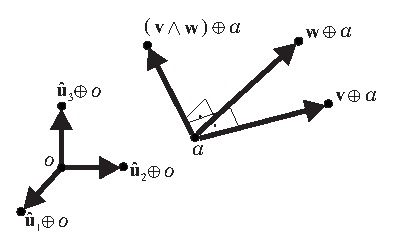
\includegraphics{partes/parte1/figs/c_geoafim/maoDireita}
\titfigura{Produto vetorial na regra da m�o
direita.}\label{fg:maoDireita}
\end{figure}
Da mesma forma, $\lpa \vto{v},\vto{w},\vto{v}\wedge\vto{w} \rpa$
obedece a regra da m�o esquerda se $\{ \vun{u}_1, \vun{u}_2,
\vun{u}_3\}$ estiver negativamente orientada.

Considerando $\eaf{V}{A}{\real}$ um espa�o afim Euclidiano, seja $\con{U}$ positivamente orientada e o conjunto $\lch\vto{u},\vto{v}, \vto{w}\rch$ linearmente independente. Utilizando a defini��o (\ref{eq:anguloProdInterno}), com base nas propriedades (\ref{eq:produtoInternoVetorial1}) e (\ref{eq:produtoTriplo}),  pode-se realizar o seguinte desenvolvimento:
\begin{eqnarray}
\vto{u}\cdot\lpa\vto{v}\wedge\vto{w}\rpa &=& \|\vto{u}\|\|\vto{v}\wedge\vto{w}\|\cos\theta_1\nonumber\\
&=& \|\vto{u}\|\sqrt{\lpa\vto{v}\wedge\vto{w}\rpa\cdot\lpa\vto{v}\wedge\vto{w}\rpa}\cos\theta_1\nonumber\\
&=& \|\vto{u}\|\sqrt{\vto{v}\cdot\lpa\vto{w}\wedge\vto{v}\wedge\vto{w}\rpa}\cos\theta_1\nonumber\\
&=& \|\vto{u}\|\sqrt{\vto{v}\cdot\lco\lpa\vto{w}\cdot\vto{w}\rpa\vto{v}-\lpa\vto{w}\cdot\vto{v}\rpa\vto{w}\rco}\cos\theta_1\nonumber\\
&=& \|\vto{u}\|\sqrt{\lco\|\vto{w}\|^2\|\vto{v}\|^2-\lpa\vto{w}\cdot\vto{v}\rpa^2 \rco}\cos\theta_1\nonumber\\
&=& \|\vto{u}\|\sqrt{\|\vto{w}\|^2\|\vto{v}\|^2\lpa 1- \cos^2\theta_2\rpa}\cos\theta_1\nonumber\\
&=& \underbrace{\|\vto{u}\|\cos\theta_1}_{\mathrm{I}}\underbrace{\|\vto{w}\|\|\vto{v}\|\sin\theta_2}_{\mathrm{II}}\,.
\end{eqnarray}
Em termos geom�tricos, esta �ltima igualdade revela que o termo destacado II � a �rea de um paralelogramo definido pelas linhas $\overline{\ele{a},\vto{w}\oplus\ele{a}}$ e $\overline{\ele{a},\vto{v}\oplus\ele{a}}\,$. O termo I, por sua vez, � o valor da dist�ncia entre  o ponto $\vto{u}\oplus\ele{a}$ e o plano $\saf{sp\lch\vto{v},\vto{w}\rch}{S}{a}{\real}$.
\begin{figure}[!ht]
\centering
\begin{center}
\input{partes/parte1/figs/c_geoafim/prodtriplo.pstex_t}
\end{center}
\titfigura{O paralelep�pedo gerado por $\vto{u}\cdot(\vto{v}\wedge\vto{w})$.}\label{fg:prodTriplo}
\end{figure}
O escalar $\vto{u}\cdot\lpa\vto{v}\wedge\vto{w}\rpa$ �, portanto, o volume do paralelep�pedo definido pelas linhas $\overline{\ele{a},\vto{w}\oplus\ele{a}}\,$, $\overline{\ele{a},\vto{v}\oplus\ele{a}}\,$ e $\overline{\ele{a},\vto{u}\oplus\ele{a}}$, conforme mostrado na figura \ref{fg:prodTriplo}.
Pelos termos da proposi��o \ref{teo:produtoTriplo}, aplicados neste contexto, pode-se dizer que o determinante de um tensor de segunda ordem � igual � raz�o do volume de um paralelep�pedo por ele modificado e o volume deste mesmo paralelep�pedo na situa��o n�o modificada.
\end{comment}

%    \chapter{Diferencia��o de Fun��es Tensoriais}

\section{Diferenciabilidade de Fun��es Tensoriais}

\subsection{Fun��o Tensorial Limitada}\index{fun��o!tensorial!limitada}
Sejam os espa�os tensoriais normados $\ete{\crt{V}{p}}{\con{F}}$ e
$\ete{\crt{W}{q}}{\con{F}}$ com as respectivas normas
$\|\bullet\|_{\ete{\crt{V}{p}}{\con{F}}}$ e
$\|\bullet\|_{\ete{\crt{W}{q}}{\con{F}}}$. A fun��o no mapeamento
\begin{equation}\label{eq:mapFuncaoLimitada}
\map{\psi}{{T}_{\con{\crt{V}{p}}\mapsto\con{\con{F}}}}{\cft{\crt{W}{q}}{\con{F}}}
\end{equation}
� dita limitada em  ${T}_{\con{\crt{V}{p}}\mapsto\con{\con{F}}}$
se existir uma constante $\Lambda\in\con{F}$ tal que
\begin{equation}
\|\fua{\psi}{\tnr{X}}\|_{\ete{\crt{W}{q}}{\con{F}}}\leqslant\Lambda\|\tnr{X}\|_{\ete{\crt{V}{p}}{\con{F}}}\,,\,
\forall\,\tnr{X}\in\cft{\crt{V}{p}}{\con{F}}\,.
\end{equation}
Das poss�veis constantes $\Lambda$ que obedecem a desigualdade
anterior, seja $\lambda$ a menor delas. Nesta situa��o, para a
fun��o $\psi$, � poss�vel definir que
\begin{equation}
\| \psi \| = \lambda\,.
\end{equation}
O conjunto de fun��es limitadas � portanto normado. Al�m disso, se
os espa�os tensoriais $\ete{\crt{V}{p}}{\con{F}}$ e
$\ete{\crt{W}{q}}{\con{F}}$ forem de Banach, toda fun��o limitada
linear � cont�nua.
\newline

\noindent\begin{prova} Vamos demonstrar agora se a �ltima
afirma��o � ver�dica. Para tal, suponhamos uma seq��ncia de Cauchy
qualquer $\lim_{i\to\infty}{\fua{\varrho}{\tnr{X}_i,\tnr{T}_0}}=0$
em ${T}_{\con{\crt{V}{p}}\mapsto\con{\con{F}}}$. Isto indica que
$\tnr{X}_i\to\tnr{T}_0$, quando $i\to\infty$. Ent�o, pode-se dizer
que $\lim_{i\to\infty}{\| \tnr{X}_i-\tnr{T}_0 \|}=0$. Com base
nisso e considerando a fun��o em ($\ref{eq:mapFuncaoLimitada}$)
limitada linear, a desigualdade
\begin{equation}
{\|\fua{\psi}{\tnr{X}_i}-\fua{\psi}{\tnr{T}_0}\|}=
{\|\fua{\psi}{\tnr{X}_i-\tnr{T}_0}\|}\leqslant\|\psi\|\|
\tnr{X}_i-\tnr{T}_0\|\,\nonumber
\end{equation}
quando $i\to\infty$, permite concluir que
$\fua{\psi}{\tnr{X}_i}\to\fua{\psi}{\tnr{T}_0}$\,.
\end{prova}



\subsection{Fun��es Tensoriais
Tangentes}\index{fun��es!tensoriais!tangentes} Dados os espa�os
tensoriais de Banach $\ete{\crt{V}{p}}{\con{F}}$ e
$\ete{\crt{W}{q}}{\con{F}}$ com as respectivas normas
$\|\bullet\|_{\ete{\crt{V}{p}}{\con{F}}}$ e
$\|\bullet\|_{\ete{\crt{W}{q}}{\con{F}}}$, seja
$\con{\tilde{T}}_{\con{\crt{V}{p}}\mapsto\con{\con{F}}}$ um
subconjunto aberto de $\cft{\crt{V}{p}}{\con{F}}$ e o mapeamento
\begin{equation}
\map{\psi}{{\tilde{T}}_{\con{\crt{V}{p}}\mapsto\con{\con{F}}}}{\cft{\crt{W}{q}}{\con{F}}}\,.
\end{equation}
Considerando um tensor
$\tnr{T}_0\in{\tilde{T}}_{\con{\crt{V}{p}}\mapsto\con{\con{F}}}$,
toda e qualquer fun��o $\kappa$, tal que
\begin{equation}
\map{\kappa}{{\tilde{T}}_{\con{\crt{V}{p}}\mapsto\con{\con{F}}}}{\cft{\crt{W}{q}}{\con{F}}}\,,
\end{equation}
� dita tangente � $\psi$ em $\tnr{T}_0$ e vice-versa se, dados o
escalar $\alpha\in\con{F}$ e um tensor qualquer n�o nulo
$\tnr{H}\in{\tilde{T}}_{\con{\crt{V}{p}}\mapsto\con{\con{F}}}$ ,
\begin{equation}\label{eq:funcaoTangenteGateaux}
\lim_{\alpha\to 0}\frac{\| \fua{\psi}{\alpha\tnr{H}+\tnr{T}_0} -
\fua{\kappa}{\alpha\tnr{H}+\tnr{T}_0}
 \|_{\ete{\crt{W}{q}}{\con{F}}}}
{\|\alpha\tnr{H}\|_{\ete{\crt{V}{p}}{\con{F}}}}=0\,.
\end{equation}
Em outras palavras, o valor no numerador aproxima-se de zero de
forma mais r�pida do que no denominador quando o tensor
$\alpha\tnr{H}\to\negmath{0}$, segundo a ``dire��o'' definida por
$\tnr{H}$. Nestas condi��es, fica evidente que,
no limite, $\fua{\psi}{\tnr{T}_0}=\fua{\kappa}{\tnr{T}_0}$. Al�m disso, se
duas fun��es s�o tangentes a $\psi$ em $\tnr{T}_0$, ent�o elas s�o
tangentes entre si.
\newline

\noindent\begin{prova} Para provar a afirma��o anterior, sejam
duas fun��es $\kappa_1$ e $\kappa_2$ tangentes a $\psi$ em
$\tnr{T}_0$. Como a soma dos limites � o limite da soma, tem-se
que
\begin{equation}
\lim_{\alpha\to 0}\frac{\| \fua{\psi}{\alpha\tnr{H}+\tnr{T}_0} -
\fua{\kappa_1}{\alpha\tnr{H}+\tnr{T}_0}
 \|_{\ete{\crt{W}{q}}{\con{F}}}+\| \fua{\kappa_2}{\alpha\tnr{H}+\tnr{T}_0}- \fua{\psi}{\alpha\tnr{H}+\tnr{T}_0}
 \|_{\ete{\crt{W}{q}}{\con{F}}}}
{\|\alpha\tnr{H}\|_{\ete{\crt{V}{p}}{\con{F}}}}=0\,. \nonumber
\end{equation}
A partir da desigualdade triangular, � certo dizer que o valor do
numerador
\begin{eqnarray}
  \lefteqn{\| \fua{\psi}{\alpha\tnr{H}+\tnr{T}_0} -
\fua{\kappa_1}{\alpha\tnr{H}+\tnr{T}_0}
 \|_{\ete{\crt{W}{q}}{\con{F}}}
+} & & \nonumber\\
  &
&\| \fua{\kappa_2}{\alpha\tnr{H}+\tnr{T}_0}-
\fua{\psi}{\alpha\tnr{H}+\tnr{T}_0}
 \|_{\ete{\crt{W}{q}}{\con{F}}}\geqslant\| \fua{\kappa_2}{\alpha\tnr{H}+\tnr{T}_0} -
\fua{\kappa_1}{\alpha\tnr{H}+\tnr{T}_0}
\|_{\ete{\crt{W}{q}}{\con{F}}}\,.\nonumber
\end{eqnarray}
Tal desigualdade permite concluir que
\begin{equation}
\lim_{\alpha\to 0}\frac{\| \fua{\kappa_2}{\alpha\tnr{H}+\tnr{T}_0}
- \fua{\kappa_1}{\alpha\tnr{H}+\tnr{T}_0}
 \|_{\ete{\crt{W}{q}}{\con{F}}}}
{\|\alpha\tnr{H}\|_{\ete{\crt{V}{p}}{\con{F}}}}=0\,. \nonumber
\end{equation}
\end{prova}

\subsubsection{Abordagens Forte e
Fraca}\index{fun��es!tensoriais!tangentes!fortes} Considerando as
condi��es anteriores, seja o conjunto $\con{TG}_{\tnr{T}_0}$
formado por pares ordenados de fun��es tangentes entre si em
$\tnr{T}_0$, cujo dom�nio � um subconjunto aberto de $\cft{\crt{V}{p}}{\con{F}}$ que cont�m $\tnr{T}_0$. Pode ocorrer que exista um conjunto
$\overline{\con{TG}}_{\tnr{T}_0}\subseteq\con{TG}_{\tnr{T}_0}$,
tal que seus pares de fun��es sejam tangentes em $\tnr{T}_0$
independente da forma como o tensor $\alpha\tnr{H}\to\negmath{0}$ em
(\ref{eq:funcaoTangenteGateaux}). Em outras palavras, considerando
$\tnr{Y}:=\alpha\tnr{H}$, para que
$(\psi,\kappa)\in\overline{\con{TG}}_{\tnr{T}_0}$, deve ser v�lida
a igualdade:
\begin{equation}\label{eq:funcaoTangenteFrechet}
\lim_{\tnr{Y}\to \negmath{0}}\frac{\| \fua{\psi}{\tnr{Y}+\tnr{T}_0} -
\fua{\kappa}{\tnr{Y}+\tnr{T}_0}
 \|_{\ete{\crt{W}{q}}{\con{F}}}}
{\|\tnr{Y}\|_{\ete{\crt{V}{p}}{\con{F}}}}=0\,.
\end{equation}
Pode-se observar que esta condi��o � mais restritiva ou mais
\emph{forte} do que a condi��o (\ref{eq:funcaoTangenteGateaux}). A
primeira � ent�o denominada abordagem forte para fun��es
tensoriais tangentes enquanto a segunda � denominada abordagem
fraca\index{fun��es!tensoriais!tangentes!fracas}. � importante
enfatizar a diferen�a entre as duas abordagens: utilizando uma
terminologia geom�trica, na abordagem fraca, o ``caminho''
trilhado pela vari�vel no dom�nio
${\tilde{T}}_{\con{\crt{V}{p}}\mapsto\con{\con{F}}}$ � definido
pelo tensor $\tnr{H}$ arbitrado; na abordagem forte, arbitra-se o
pr�prio ``caminho'' a ser trilhado. Para fins did�ticos, os
``caminhos'' em ambas as abordagens est�o representados na figura
a seguir.

\begin{figure}[!htt]
\centering
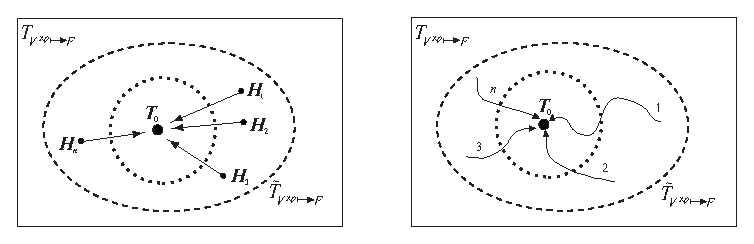
\includegraphics{partes/parte1/figs/c_diftens/AbordagemForteFraca.eps}
\titfigura{� esquerda, abordagem fraca com tensores arbitr�rios e
``caminhos'' radiais. � direita, abordagem forte com ``caminhos''
arbitr�rios.}
\end{figure}

Cabe ressaltar que se o dom�nio tensorial das fun��es tangentes
for unidimensional (independente da ordem), as abordagens forte e
fraca ficam id�nticas. Desta forma,
\begin{eqnarray}
\dim\lpa\ete{\crt{V}{p}}{\con{F}}\rpa=1&\implies &
\overline{\con{TG}}_{\tnr{T}_0}=\con{TG}_{\tnr{T}_0}\,.\nonumber
\end{eqnarray}

\noindent\begin{prova} Para o caso do espa�o tensorial unidimensional $\ete{\crt{V}{p}}{\con{F}}$, seja o conjunto $\lch\tnr{H}\rch$ uma de suas bases. Neste contexto, o tensor $\tnr{Y}$ em (\ref{eq:funcaoTangenteFrechet}) pode sempre ser escrito como a combina��o linear $\alpha\tnr{H}$, resultando assim a express�o (\ref{eq:funcaoTangenteGateaux}).
\end{prova}

\subsection{Diferenciabilidade de G�teaux}\index{G�teaux!diferenciabilidade de}
Sejam os espa�os tensoriais de Banach $\ete{\crt{V}{p}}{\con{F}}$
e $\ete{\crt{W}{q}}{\con{F}}$ e o espa�o vetorial de fun��es
tensoriais lineares
\begin{equation}
\evl{\cft{\crt{V}{p}}{\con{F}}}{\cft{\crt{W}{q}}{\con{F}}}{\con{F}}\,.\nonumber
\end{equation}
Considerando ${\tilde{T}}_{\con{\crt{V}{p}}\mapsto\con{\con{F}}}$
um subconjunto aberto de $\cft{\crt{V}{p}}{\con{F}}$, seja um
tensor
$\tnr{T}_0\in{\tilde{T}}_{\con{\crt{V}{p}}\mapsto\con{\con{F}}}$ e
o conjunto dos pares ordenados de fun��es tensoriais tangentes
$\con{TG}_{\tnr{T}_0}$. Dado o mapeamento
\begin{equation}
\map{\psi}{{\tilde{T}}_{\con{\crt{V}{p}}\mapsto\con{\con{F}}}}{\cft{\crt{W}{q}}{\con{F}}}\,,
\end{equation}
se existir o par de fun��es tangentes
$(\psi,\psi_D)\in\con{TG}_{\tnr{T}_0}$, onde
\begin{equation}\label{eq:funcaoGDerivada}
\fua{\psi_D}{\tnr{X}}=\fua{\psi}{\tnr{T}_0}+\fua{\lco\fua{\dvt{\psi}}{\tnr{T}_0}\rco}{\tnr{X}-\tnr{T}_0}\,,
\end{equation}
tal que a fun��o
\begin{equation}
\lco\fua{\dvt{\psi}}{\tnr{T}_0}\rco\in
\cfl{\cft{\crt{V}{p}}{\con{F}}}{\cft{\crt{W}{q}}{\con{F}}}
\end{equation}
� limitada, ent�o este par � �nico. Nestas condi��es, a fun��o
$\psi$ � dita \emph{diferenci�vel de G�teaux}\index{G�teaux!fun��o
diferenci�vel de} ou
\emph{G-diferenci�vel}\index{fun��o!G-diferenci�vel} em
$\tnr{T}_0$. Combinando (\ref{eq:funcaoGDerivada}) com
(\ref{eq:funcaoTangenteGateaux}), obt�m-se que
\begin{equation}\label{eq:derivadaGateauxIni}
\lim_{\alpha\to 0}\frac{\|
\fua{\psi}{\alpha\tnr{\tnr{H}}+\tnr{T}_0} - \fua{\psi}{\tnr{T}_0}-
\alpha\fua{\lco\fua{\dvt{\psi}}{\tnr{T}_0}\rco}{\tnr{H}}
 \|_{\ete{\crt{W}{q}}{\con{F}}}}
{\|\alpha\tnr{H}\|_{\ete{\crt{V}{p}}{\con{F}}}}=0\,.
\end{equation}
O termo $\alpha\fua{\lco\fua{\dvt{\psi}}{\tnr{T}_0}\rco}{\tnr{H}}$
� denominado o \emph{diferencial de
G�teaux}\index{G�teaux!diferencial de} ou o
\emph{G-diferencial}\index{G-diferencial} de $\psi$ em $\tnr{T}_0$
na dire��o $\tnr{H}$. Chama-se o tensor
$\fua{\lco\fua{\dvt{\psi}}{\tnr{T}_0}\rco}{\tnr{H}}$ de
\emph{derivada direcional}\index{derivada!direcional} de $\psi$ em
$\tnr{T}_0$ na dire��o $\tnr{H}$. A fun��o tensorial linear
limitada $\lco\fua{\dvt{\psi}}{\tnr{T}_0}\rco$ � chamada
\emph{derivada fraca}\index{derivada!fraca} ou \emph{derivada de
G�teaux}\index{G�teaux!derivada de} ou
\emph{G-derivada}\index{G-derivada} de $\psi$ em $\tnr{T}_0$. A fun��o $\dvt{\psi}$ � denominada simplesmente a derivada de
G�teaux ou a G-derivada de $\psi$. Al�m disso, se a
fun��o $\psi$ for G-diferenci�vel em qualquer tensor $\tnr{T}_0$
do seu dom�nio, diz-se que ela � G-diferenci�vel em
${\tilde{T}}_{\con{\crt{V}{p}}\mapsto\con{\con{F}}}$.
\newline

\noindent\begin{prova} Vamos mostrar que a fun��o $\psi_D$ �
�nica. Para tal, admitamos, por hip�tese, que existam duas fun��es
$\psi_{D1}$ e $\psi_{D2}$ tangentes � $\psi$ em $\tnr{T}_0$, tais
que
\begin{equation}
\fua{\psi_{D1}}{\tnr{X}}=
\fua{\psi}{\tnr{T}_0}+\fua{\lco\fua{\dvt{\psi_1}}{\tnr{T}_0}\rco}{\tnr{X}-\tnr{T}_0}\nonumber
\end{equation}
e
\begin{equation}
\fua{\psi_{D2}}{\tnr{X}}=
\fua{\psi}{\tnr{T}_0}+\fua{\lco\fua{\dvt{\psi_2}}{\tnr{T}_0}\rco}{\tnr{X}-\tnr{T}_0}\,.\nonumber
\end{equation}
Desta forma, $\psi_{D1}$ e $\psi_{D2}$ s�o tangentes entre si em
$\tnr{T}_0$. Aplicando a abordagem fraca de fun��es tangentes,
obt�m-se que
\begin{eqnarray}
\lim_{\alpha\to 0}\frac{\|
\fua{\lco\fua{\dvt{\psi_1}}{\tnr{T}_0}\rco}{\alpha\tnr{H}} -
\fua{\lco\fua{\dvt{\psi_2}}{\tnr{T}_0}\rco}{\alpha\tnr{H}}
 \|_{\ete{\crt{W}{q}}{\con{F}}}}
{\|\alpha\tnr{H}\|_{\ete{\crt{V}{p}}{\con{F}}}}&=&0\,.\nonumber
\end{eqnarray}
Elimina-se, pelas propriedades de fun��es lineares e normas, o
escalar $\alpha$. Logo,
\begin{equation}
\frac{\|
\fua{\lco\fua{\dvt{\psi_1}}{\tnr{T}_0}-\fua{\dvt{\psi_2}}{\tnr{T}_0}\rco}{\tnr{H}}
 \|_{\ete{\crt{W}{q}}{\con{F}}}}
{\|\tnr{H}\|_{\ete{\crt{V}{p}}{\con{F}}}} = 0\,.\nonumber
\end{equation}
Como $\tnr{H}$, por defini��o, � n�o nulo, a igualdade anterior � v�lida se o numerador for zero. Logo, � poss�vel dizer que para qualquer $\tnr{H}\in{\tilde{T}}_{\con{\crt{V}{p}}\mapsto\con{\con{F}}}$ n�o nulo,
\begin{equation}
\fua{\lco\fua{\dvt{\psi_1}}{\tnr{T}_0}\rco}{\tnr{H}}=
\fua{\lco\fua{\dvt{\psi_2}}{\tnr{T}_0}\rco}{\tnr{H}}\,.
\nonumber
\end{equation}
\end{prova}

\subsubsection{Diferenciabilidade de Ordem Arbitr�ria}
Considerando as condi��es anteriores, sejam o espa�o tensorial
$\ete{\lpa\crt{V}{p}\rpa^{k+1}}{\con{F}}$ e o espa�o tensorial de fun��es lineares
\begin{equation}
\evl{\cft{\lpa\crt{V}{p}\rpa^{k+1}}{\con{F}}}{\cft{\crt{W}{q}}{\con{F}}}{\con{F}}\,,\nonumber
\end{equation}
onde $k\geqslant 0$. Considerando $\fua{\dtg{0}{\psi}}{\tnr{T}_0}:=\psi$, se existir o par ordenado de fun��es tensoriais $\lpa \fua{\dtg{k}{\psi}}{\tnr{T}_0},\psi_{\con{D}^{k+1}} \rpa\in\con{TG}_{\tnr{T}_0}$, tal que
\begin{eqnarray}
  \lefteqn{\fua{\psi_{D^{k+1}}}{\tnr{X}}=\fua{\lco\fua{\dtg{k}{\psi}}{\tnr{T}_0}\rco}{\tnr{H}_1\otimes\cdots\otimes\tnr{H}_{k-1}\otimes\tnr{T}_0}+} & & \nonumber\\
  &
&\fua{\lco\fua{\dtg{k+1}{\psi}}{\tnr{T}_0}\rco}{\tnr{H}_1\otimes\cdots\otimes\tnr{H}_{k}\otimes\lpa\tnr{X}-\tnr{T}_0\rpa}\,,
\end{eqnarray}
onde $\tnr{H}_i\in{\tilde{T}}_{\con{\crt{V}{p}}\mapsto\con{\con{F}}}$ e a fun��o
\begin{equation}
\lco\fua{\dtg{k+1}{\psi}}{\tnr{T}_0}\rco\in
\cfl{\cft{\lpa\crt{V}{p}\rpa^{k+1}}{\con{F}}}{\cft{\crt{W}{q}}{\con{F}}}
\end{equation}
� limitada, ent�o este par � �nico.

Neste contexto, diz-se que $\psi$ � G-diferenci�vel de ordem $k+1$ em $\tnr{T}_0$. A fun��o linear $\fua{\dtg{k+1}{\psi}}{\tnr{T}_0}$ � a G-derivada de ordem $k+1$ de $\psi$ em $\tnr{T}_0$. Em termos gen�ricos, a igualdade (\ref{eq:derivadaGateauxIni}) assume a seguinte forma:
\begin{equation}
\begin{array}{rrr}\label{eq:derivadaGateauxGenerica}
&\lim_{\alpha\to
0}\frac{1}{\|\alpha\tnr{H}\|_{\ete{\crt{V}{p}}{\con{F}}}} \| \fua{\lco\fua{\dtg{k}{\psi}}{\tnr{T}_0}\rco}{\tnr{H}_1\otimes\cdots\otimes\tnr{H}_{k-1}\otimes\lpa\alpha\tnr{H}+\tnr{T}_0\rpa}- & \\
&\fua{\lco\fua{\dtg{k}{\psi}}{\tnr{T}_0}\rco}{\tnr{H}_1\otimes\cdots\otimes\tnr{H}_{k-1}\otimes\tnr{T}_0}- &
\\  &
\alpha\fua{\lco\fua{\dtg{k+1}{\psi}}{\tnr{T}_0}\rco}{\tnr{H}_1\otimes\cdots\otimes\tnr{H}_{k}\otimes\tnr{H}}\|_{\ete{\crt{W}{q}}{\con{F}}}=0\,. &
\end{array}
\end{equation}





\subsubsection{Diferenciabilidade de Fr�chet}\index{Fr�chet!diferenciabilidade de}
Considerando as condi��es anteriores, se agora existir o par de
fun��es tangentes
$(\psi,\psi_D)\in\overline{\con{TG}}_{\tnr{T}_0}$, ent�o a fun��o
$\psi$ � dita \emph{diferenci�vel de Fr�chet}\index{Fr�chet!fun��o
diferenci�vel de} ou
\emph{F-diferenci�vel}\index{fun��o!F-diferenci�vel} em
$\tnr{T}_0$. Combinando (\ref{eq:funcaoGDerivada}) e
(\ref{eq:funcaoTangenteFrechet}), obt�m-se
\begin{equation}
\lim_{\tnr{Y}\to \negmath{0}}\frac{\|
\fua{\psi}{\tnr{\tnr{Y}}+\tnr{T}_0} - \fua{\psi}{\tnr{T}_0}-
\fua{\lco\fua{\dvt{\psi}}{\tnr{T}_0}\rco}{\tnr{Y}}
 \|_{\ete{\crt{W}{q}}{\con{F}}}}
{\|\tnr{Y}\|_{\ete{\crt{V}{p}}{\con{F}}}}=0\,.
\end{equation}
O tensor $\fua{\lco\fua{\dvt{\psi}}{\tnr{T}_0}\rco}{\tnr{Y}}$ �
denominado o \emph{diferencial de
Fr�chet}\index{Fr�chet!diferencial de} ou o
\emph{F-di\-fe\-ren\-cial}\index{F-diferencial} de $\psi$ em
$\tnr{T}_0$. A fun��o tensorial limitada linear
$\lco\fua{\dvt{\psi}}{\tnr{T}_0}\rco$ � chamada \emph{derivada
forte}\index{derivada!forte} ou \emph{derivada de
Fr�chet}\index{Fr�chet!derivada de} ou
\emph{F-derivada}\index{F-derivada}\footnote{A demonstra��o de que
a F-derivada � �nica pode ser feita utilizando a mesma metodologia
aplicada � G-derivada, substituindo as ocorr�ncias de $\tnr{Y}$
por $\alpha\tnr{H}$ em (\ref{eq:funcaoTangenteFrechet}).} de
$\psi$ em $\tnr{T}_0$. A fun��o $\dvt{\psi}$ � a derivada de Fr�chet ou a F-derivada de $\psi$.

Conv�m enfatizar que uma fun��o F-diferenci�vel � sempre
G-di\-fe\-ren\-ci�\-vel\footnote{Uma fun��o
G-di\-fe\-ren\-ci�\-vel � sempre F-diferenci�vel em condi��es
especiais. Ver \aut{Wouk}\cite{wouk_1979_1}, pp. 268-270.} e suas
derivadas respectivas s�o iguais. Apesar disso, � conveniente
utilizar nota��es diferentes para cada uma das derivadas: as
derivadas $\fua{\dvf{\psi}}{\tnr{T}_0}$ e
$\fua{\dvg{\psi}}{\tnr{T}_0}$ indicam, respectivamente, que $\psi$
� F-diferenci�vel e G-diferenci�vel em $\tnr{T}_0$. Caso $\psi$
seja F ou G-diferenci�vel no seu dom�nio, ent�o as nota��es
respectivas para as derivadas s�o $\fua{\dvf{\psi}}{\tnr{X}}$ e
$\fua{\dvg{\psi}}{\tnr{X}}$.

O conceito de derivadas de ordens superiores tamb�m � extens�vel � abordagem forte de fun��es tangentes. Desta forma, diz-se que $\fua{\dgg{k}{\psi}}{\tnr{T}_0}$ e $\fua{\dgf{k}{\psi}}{\tnr{T}_0}$ s�o respectivamente a G-derivada e a F-derivada de ordem $k$ de $\psi$ em $\tnr{T}_0$.

\subsubsection{Calculando a Derivada Direcional}
Ainda sob as condi��es anteriores, a igualdade
(\ref{eq:derivadaGateauxIni}) revela que o numerador aproxima-se mais r�pido de $0$ do que o denominador.
Desta forma, � poss�vel concluir que
\begin{equation}\label{eq:numeradorGateaux}
\lim_{\alpha\to 0}\lco\fua{\psi}{\alpha\tnr{\tnr{H}}+\tnr{T}_0} - \fua{\psi}{\tnr{T}_0}-
\alpha\fua{\lco\fua{\dvg{\psi}}{\tnr{T}_0}\rco}{\tnr{H}}\rco
 =\negmath{0}\,.
\end{equation}
J� que $\alpha$ nunca � $0$, o termo entre colchetes nesta express�o nunca � zero, ou seja, sempre h� um \emph{res�duo}. Tal res�duo pode ser definido pela fun��o tensorial no mapeamento
\begin{equation}
\map{\ele{r}_\psi}{{\tilde{T}}_{\con{\crt{V}{p}}\mapsto\con{\con{F}}}}{\cft{\crt{W}{q}}{\con{F}}}\,,
\end{equation}
onde
\begin{equation}
\lim_{\tnr{X}\to \negmath{0}}\fua{\ele{r}_\psi}{\tnr{X}}=\negmath{0}\,.
\end{equation}
Com base nisso, pode-se entender a express�o
(\ref{eq:numeradorGateaux}) segundo a igualdade
\begin{equation}\label{eq:gderivadaResiduo}
\fua{\psi}{\alpha\tnr{\tnr{H}}+\tnr{T}_0} - \fua{\psi}{\tnr{T}_0}-
\alpha\fua{\lco\fua{\dvg{\psi}}{\tnr{T}_0}\rco}{\tnr{H}}
 = \fua{\ele{r}_\psi}{\tnr{H}}\,,
\end{equation}
onde $\ele{r}_\psi$ � dita a \emph{fun��o
res�duo}\index{fun��o!res�duo} de $\psi$ em $\tnr{T}_0\,$.
Neste contexto, isolando o termo da derivada direcional na igualdade anterior e em seguida aplicando $\lim_{\alpha\to 0}$ em ambos os lados da express�o resultante, obt�m-se que
\begin{equation}\label{eq:calculoDerivadaDirecional}
\fua{\lco\fua{\dvg{\psi}}{\tnr{T}_0}\rco}{\tnr{H}} =
\lim_{\alpha\to 0}\frac{\fua{\psi}{\alpha\tnr{\tnr{H}}+\tnr{T}_0}
- \fua{\psi}{\tnr{T}_0}}{\alpha}\,.
\end{equation}
Vale ressaltar que para qualquer $\tnr{H}$, esta igualdade fornece
uma regra para a derivada $\fua{\dvg{\psi}}{\tnr{T}_0}$. Al�m disso, se $\tnr{T}_0$ tamb�m for um tensor qualquer, ou seja, se $\psi$ for G-diferenci�vel no seu dom�nio, tem-se a regra para a derivada direcional de $\psi$.

COLOCAR UMA PROPOSI��O QUE MOSTRE A DERIVADA DIRECIONAL DE UMA FUN��O ESCALAR

\paragraph{Derivadas Direcionais de Ordem Arbitr�ria.} O c�lculo da
derivada direcional de ordem $k+1$, $k\geqslant 0$, �
feito a partir de (\ref{eq:derivadaGateauxGenerica}), generalizando a igualdade
(\ref{eq:calculoDerivadaDirecional}). Desta forma,
\begin{eqnarray}\label{eq:calculoDerivadaDirecionalOrdemN}
  \lefteqn{\fua{\lco\fua{\dgg{k+1}{\psi}}{\tnr{T}_0}\rco}{\tnr{H}_1\otimes\cdots\otimes\tnr{H}_{k}\otimes\tnr{H}}
=\lim_{\alpha\to
0}\frac{1}{\alpha}} & & \nonumber\\
  &
&\fua{\lco\fua{\dgg{k}{\psi}}{\tnr{T}_0}\rco}{\tnr{H}_1\otimes\cdots\otimes\tnr{H}_{k-1}\otimes\lpa \alpha\tnr{\tnr{H}}+\tnr{T}_0\rpa}
-\nonumber\\  & &
\qquad\fua{\lco\fua{\dgg{k}{\psi}}{\tnr{T}_0}\rco}{\tnr{H}_1\otimes\cdots\otimes\tnr{H}_{k-1}\otimes\tnr{T}_0}\,,
\end{eqnarray}
onde
$\tnr{H}_i\in{\tilde{T}}_{\con{\crt{V}{p}}\mapsto\con{\con{F}}}$ e
$\fua{\dgg{0}{\psi}}{\tnr{T}_0}:=\psi\,$. Para tensores
$\tnr{H},\tnr{H}_1,\cdots,\tnr{H}_k$ quaisquer, obt�m-se a regra
da G-derivada $\fua{\dgg{k+1}{\psi}}{\tnr{T}_0}$ e por
conseq��ncia da F-derivada $\fua{\dgf{k+1}{\psi}}{\tnr{T}_0}$.

\paragraph{Derivadas Parciais.}\index{derivada!parcial}\label{sec:derivadaParcial}
Considerando as condi��es anteriores, seja o inteiro $m\geqslant 1$ e o conjunto
\begin{equation}
\con{P}={T}_{\con{\crt{V}{p_1}}\mapsto\con{\con{F}}}\times\cdots\times{T}_{\con{\crt{V}{p_m}}\mapsto\con{\con{F}}}
\end{equation}
definidor de um espa�o vetorial de Banach. Seja o mapeamento
\begin{equation}
\map{\omega}{\tilde{\con{P}}}{\cft{\crt{W}{q}}{\con{F}}}\,.
\end{equation}
onde $\tilde{\con{P}}$ � subconjunto aberto de $\con{P}\,$.

Com base na proposi��o \ref{prp:somaPoliadicos}, a condi��o de exist�ncia da fun��o no mapeamento anterior � garantida se, por exemplo,
\begin{equation}
\fua{\omega}{\tnr{X}_1,\cdots,\tnr{X}_m}=
\fua{\psi}{\sum_{k=1}^m\underbrace{\vto{x}_{1k}\otimes\cdots\otimes\vto{x}_{pk}}_{\tnr{X}_k}}\,,
\end{equation}
onde $p=p_1=\cdots=p_m\,$. A derivada direcional (\ref{eq:calculoDerivadaDirecional}) toma ent�o a seguinte forma gen�rica:
\begin{eqnarray}\label{eq:derivadaDirecionalVariasVariaveis}
\lefteqn{\fua{\lco\fua{\dvg{\omega}}{\tnr{T}_1,\cdots,\tnr{T}_m}\rco}{\tnr{H}_1,\cdots,\tnr{H}_m} =\lim_{\alpha\to 0}\frac{1}{\alpha}} & & \nonumber\\
& &
\fua{\omega}{\alpha\tnr{H}_1+\tnr{T}_1,\cdots,\alpha\tnr{H}_m+\tnr{T}_m}
- \fua{\omega}{\tnr{T}_1,\cdots,\tnr{T}_m}\,.
\end{eqnarray}
A partir da�, diz-se que a fun��o no lado esquerdo da igualdade
\begin{eqnarray}\label{eq:derivadaDirecionalParcial}
\lefteqn{\fua{\lco\fua{\dvg{\omega}}{\tnr{T}_1,\cdots,\tnr{T}_m}\rco}{\tnr{H}_r} =\lim_{\alpha\to
0}\frac{1}{\alpha}} & & \nonumber\\
& &
\fua{\omega}{\tnr{T}_1,\cdots,\alpha\tnr{H}_r+\tnr{T}_r,\cdots,\tnr{T}_m}
- \fua{\omega}{\tnr{T}_1,\cdots,\tnr{T}_m}
\end{eqnarray}
� a G-derivada parcial de $\omega$ em $\tnr{T}_r\,$. Neste caso, a fun��o $\dvg{\omega}$ fica representada por $\dvp{r}{\omega}$, onde $\mathrm{r}$ � o �ndice do elemento da tupla sobre o qual a derivada parcial � definida. Vale lembrar que os conceitos aqui apresentadas tamb�m s�o v�lidos no contexto da fun��o $\psi$ F-diferenci�vel.

\begin{prp}\label{teo:derivadaParcial}
Sejam os espa�os de Banach $\ebh{P}{F}$ e $\ete{\crt{V}{p_i}}{\con{F}}$ tais que o conjunto
\begin{equation*}
\con{P}:={T}_{\con{\crt{V}{p_1}}\mapsto\con{\con{F}}}\times\cdots\times{T}_{\con{\crt{V}{p_m}}\mapsto\con{\con{F}}}\,,
\end{equation*}
onde $m\geqslant 1$. Dados um espa�o tensorial $\ete{\crt{W}{q}}{\con{F}}$ e $\tilde{\con{P}}$ um subconjunto aberto de $\con{P}\,$, seja a fun��o em  $\map{\omega}{\tilde{\con{P}}}{\cft{\crt{W}{q}}{\con{F}}}$ G-diferenci�vel na tupla ordenada $(\tnr{T}_1,\cdots,\tnr{T}_m)\,$. Nestas condi��es, para qualquer elemento   $(\tnr{H}_1,\cdots,\tnr{H}_m)\in\tilde{\con{P}}\,$, a derivada direcional
\begin{equation*}
\fua{\lco\fua{\dvg{\omega}}{\tnr{T}_1,\cdots,\tnr{T}_m}\rco}{\tnr{H}_1,\cdots,\tnr{H}_m} =
\sum_{r=1}^{m}\fua{\lco\fua{\dvp{r}{\omega}}{\tnr{T}_1,\cdots,\tnr{T}_m}\rco}{\tnr{H}_r}\,.
\end{equation*}
\end{prp}
\begin{prova}\rodape{Adaptada de \aut{Zeidler}\cite{zeidler_1995_1}, pp. 232-233.}
O processo mostrado a seguir, que utiliza $m=2\,$, pode ser generalizado para valores maiores. Tomando as defini��es (\ref{eq:derivadaDirecionalVariasVariaveis}) e (\ref{eq:derivadaDirecionalParcial}), concluimos facilmente as igualdades
\begin{equation*}
\fua{\lco\fua{\dvg{\omega}}{\tnr{T}_1,\tnr{T}_2}\rco}{\tnr{H}_1,\negmath{0}}=\fua{\lco\fua{\dvp{1}{\omega}}{\tnr{T}_1,\tnr{T}_2}\rco}{\tnr{H}_1}
\end{equation*}
e
\begin{equation*}
\fua{\lco\fua{\dvg{\omega}}{\tnr{T}_1,\tnr{T}_2}\rco}{\negmath{0},\tnr{H}_2}=\fua{\lco\fua{\dvp{2}{\omega}}{\tnr{T}_1,\tnr{T}_2}\rco}{\tnr{H}_2}\,,
\end{equation*}
rotuladas respectivamente por (i) e (ii). Somando estas duas express�es, chegamos � igualdade (iii)
\begin{equation*}
\fua{\lco\fua{\dvg{\omega}}{\tnr{T}_1,\tnr{T}_2}\rco}{\lpa\tnr{H}_1,\negmath{0}\rpa+\lpa\negmath{0},\tnr{H}_2\rpa}=\fua{\lco\fua{\dvp{1}{\omega}}{\tnr{T}_1,\tnr{T}_2}\rco}{\tnr{H}_1}+\fua{\lco\fua{\dvp{2}{\omega}}{\tnr{T}_1,\tnr{T}_2}\rco}{\tnr{H}_2}\,,
\end{equation*}
v�lida para quaisquer $\tnr{H}_1,\tnr{H}_2\in\tilde{\con{P}}\,$. Como estamos tratando com espa�os vetoriais, fica claro que a tupla ordenada  $(\tnr{Z}_1,\tnr{Z}_2):=(\tnr{H}_1,\negmath{0})+(\negmath{0},\tnr{H}_2)\,$ � elemento de $\con{P}$. Fazendo $\tnr{H}_2=\negmath{0}$ em (iii), obtemos de (i) que $(\tnr{Z}_1,\tnr{Z}_2)=(\tnr{H}_1,\negmath{0})\,$. Da mesma forma, se $\tnr{H}_1=\negmath{0}\,$, obtemos de (ii) e (iii) que  $(\tnr{Z}_1,\tnr{Z}_2)=(\negmath{0},\tnr{H}_2)\,$. Como estas duas situa��es confirmam-se mutuamente, fica �bvio que $(\tnr{Z}_1,\tnr{Z}_2)=(\tnr{H}_1,\tnr{H}_2)\,$ para quaisquer $\tnr{H}_1,\tnr{H}_2\in\tilde{\con{P}}\,$.
\end{prova}

\subsection{Fun��es Tensoriais Suaves}\index{fun��o!tensorial!suave}
Sejam os espa�os tensoriais de Banach $\ete{\crt{V}{p}}{\con{F}}$
e $\ete{\crt{W}{q}}{\con{F}}$ e o subconjunto aberto
${\tilde{T}}_{\con{\crt{V}{p}}\mapsto\con{\con{F}}}\subset\cft{\crt{V}{p}}{\con{F}}$.
Sejam os conjuntos $\mathcal{C}_\mathrm{G}^0$, formado por todas as fun��es cont�nuas em seu dom�nio, e $\mathcal{D}_\mathrm{G}^1$, formado por todas as
fun��es G-diferenci�veis de ordem $1$ em seu dom�nio. Considerando
uma fun��o qualquer $\psi\in\con\mathcal{D}_\mathrm{G}^1$ que
mapeia
${\tilde{T}}_{\con{\crt{V}{p}}\mapsto\con{\con{F}}}\mapsto\con{\cft{\crt{W}{q}}{\con{F}}}$,
a G-derivada $\dvg{\psi}$ define o mapeamento
\begin{equation}
\map{\dvg{\psi}}{{\tilde{T}}_{\con{\crt{V}{p}}\mapsto\con{\con{F}}}}
{\con{LB}_{{\tilde{T}}_{\con{\crt{V}{p}}\mapsto\con{\con{F}}}\mapsto\cft{\crt{W}{q}}{\con{F}}}}
 \,,
\end{equation}
onde o conjunto
\begin{equation}
\con{LB}_{{\tilde{T}}_{\con{\crt{V}{p}}\mapsto\con{\con{F}}}\mapsto\cft{\crt{W}{q}}{\con{F}}}\subset
\cfl{\cft{\crt{V}{p}}{\con{F}}}{\cft{\crt{W}{q}}{\con{F}}}
\end{equation}
�, por defini��o, normado. Neste contexto, caso as fun��es $\psi$ e $\dvg{\psi}$ sejam
elementos de $\mathcal{C}_\mathrm{G}^0$, diz-se que $\psi$ tamb�m � elemento do conjunto
$\sug{1}\subset\mathcal{D}_\mathrm{G}^1$, formado por todas as
fun��es cont�nuas cuja G-derivada � cont�nua. � comum dizer tamb�m
que $\psi$ � de classe $\sug{1}$ ou que � G-suave de ordem 1. Da
mesma forma, para o caso de fun��es F-diferenci�veis, define-se o
conjunto $\suf{1}\subset\mathcal{D}_\mathrm{F}$ das fun��es cuja
\emph{F-derivada} � cont�nua.

Em termos gerais, para que a fun��o $\psi$ seja G-suave de ordem
$k+1$, ou da classe $\sug{k+1}$, ela e sua G-derivada
$\dgg{k}{\psi}$ devem ser G-suaves de ordem $k$. Em
outras palavras,
\begin{equation}
\psi\in\sug{k}\,\,\mathrm{e}\,\,\dgg{k}{\psi}\in\sug{k}\Longleftrightarrow\psi\in\sug{k+1}\,,\,\,k\geqslant
0\,.
\end{equation}

\subsubsection{Difeomorfismo}\index{difeomorfismo} Considerando as condi��es anteriores,
dado um tensor
$\tnr{T}_0\in{\tilde{T}}_{\con{\crt{V}{p}}\mapsto\con{\con{F}}}$,
a fun��o tensorial $\psi$ � um difeomorfismo em $\tnr{T}_0$ se ela
for uma bije��o G-diferenci�vel em $\tnr{T}_0$ e sua fun��o
inversa for G-diferenci�vel em $\fua{\psi}{\tnr{T}_0}$. Se a
bije��o $\psi$ e sua inversa forem G-suaves de ordem $n$, ent�o diz-se que $\psi$ � um
\emph{$\sug{n}$-difeomorfismo}.

\begin{teo}[Fun��o Inversa Local]\index{Fun��o Inversa Local!Teorema da}\label{teo:FuncaoInversaLocal}
Sejam os espa�os tensoriais de Banach $\ete{\crt{V}{p}}{\con{F}}$
e $\ete{\crt{W}{q}}{\con{F}}$. Seja o subconjunto aberto
${\tilde{T}}_{\con{\crt{V}{p}}\mapsto\con{\con{F}}}\subset\cft{\crt{V}{p}}{\con{F}}$
e um tensor
$\tnr{T}_0\in{\tilde{T}}_{\con{\crt{V}{p}}\mapsto\con{\con{F}}}$.
Uma fun��o tensorial $\psi$ � um $\sug{n}$-difeomorfismo em
$\tnr{T}_0$ se e somente se sua derivada
$\fua{\dvg{\psi}}{\tnr{T}_0}$ for uma bije��o.
\end{teo}
\begin{prova}
Este teorema � uma aplica��o do Teorema da Fun��o
Impl�cita\rodape{Ver \aut{Zeidler}\cite{zeidler_1995_1}, pp.
259-260.}.
\end{prova}


\subsection{Regras Fundamentais Para Derivadas}
S�o apresentadas a seguir algumas regras aqui consideradas
fundamentais nos procedimentos de obten��o de derivadas. A
abordagem aplicada para se conseguir tais regras faz uso do
c�lculo da derivada direcional, considerando o argumento de
dire��o um tensor qualquer.

\begin{teo}[Regra da Soma]\index{Regra da Soma}\label{teo:RegraSome}
Sejam os espa�os tensoriais de Banach $\ete{\crt{V}{p}}{\con{F}}$ e
$\ete{\crt{W}{q}}{\con{F}}$. Seja o subconjunto aberto
${\tilde{T}}_{\con{\crt{V}{p}}\mapsto\con{\con{F}}}\subset\cft{\crt{V}{p}}{\con{F}}$.
Sejam as fun��es $\psi$, $\psi_1$ e $\psi_2$ que mapeiam
${\tilde{T}}_{\con{\crt{V}{p}}\mapsto\con{\con{F}}}\mapsto\cft{\crt{W}{q}}{\con{F}}$. Se
$\psi$ for G-diferenci�vel no seu dom�nio com regra
\begin{equation}
\fua{\psi}{\tnr{X}}=\fua{\psi_1}{\tnr{X}}+\fua{\psi_2}{\tnr{X}}\,,\nonumber
\end{equation}
ent�o a fun��o
\begin{equation}
\fua{\dvg{\psi}}{\tnr{X}}=\fua{\dvg{\psi_1}}{\tnr{X}}+
\fua{\dvg{\psi_2}}{\tnr{X}}\,.\nonumber
\end{equation}
\end{teo}
\begin{prova}
Considerando o tensor $\tnr{H}\in{\tilde{T}}_{\con{\crt{V}{p}}\mapsto\con{\con{F}}}$ uma
dire��o qualquer, seja o seguinte desenvolvimento:
\begin{eqnarray}
\fua{\lco\fua{\dvg{\psi}}{\tnr{X}}\rco}{\tnr{H}}&=&
\lim_{\alpha\to
0}\frac{\fua{\psi_1}{\alpha\tnr{\tnr{H}}+\tnr{X}}+\fua{\psi_2}{\alpha\tnr{\tnr{H}}+\tnr{X}}
- \fua{\psi_1}{\tnr{X}}-\fua{\psi_2}{\tnr{X}}}{\alpha} \nonumber\\
&=&\lim_{\alpha\to 0}\frac{\fua{\psi_1}{\alpha\tnr{\tnr{H}}+\tnr{X}} -
\fua{\psi_1}{\tnr{X}}}{\alpha}+\lim_{\alpha\to
0}\frac{\fua{\psi_2}{\alpha\tnr{\tnr{H}}+\tnr{X}} - \fua{\psi_2}{\tnr{X}}}{\alpha}
\nonumber\\
&=&\fua{\lco\fua{\dvg{\psi_1}}{\tnr{X}}\rco}{\tnr{H}}+\fua{\lco\fua{\dvg{\psi_2}}{\tnr{X}}\rco}{\tnr{H}}\nonumber\\
&=&\fua{\lco\fua{\dvg{\psi_1}}{\tnr{X}}+\fua{\dvg{\psi_2}}{\tnr{X}}\rco}{\tnr{H}}\,.\nonumber
\end{eqnarray}
A �ltima igualdade � obtida porque as derivadas $\fua{\dvg{\psi_1}}{\tnr{X}}$ e
$\fua{\dvg{\psi_2}}{\tnr{X}}$ s�o elementos de um espa�o vetorial de fun��es lineares.
\end{prova}

\begin{teo}[Regra do Produto]\index{Regra do Produto}\label{teo:RegraProduto}
Sejam os quatro espa�os tensoriais de Banach
$\ete{\crt{V}{p}}{\con{F}}$,
$\ete{\crt{K}{r}\times\crt{Z}{s}}{\con{F}}$,
$\ete{\crt{K}{r}\times\crt{W}{q}}{\con{F}}$ e
$\ete{\crt{W}{q}\times\crt{Z}{s}}{\con{F}}$. Sejam o subconjunto
aberto
${\tilde{T}}_{\con{\crt{V}{p}}\mapsto\con{\con{F}}}\subset\cft{\crt{V}{p}}{\con{F}}$
e os mapeamentos:
\begin{eqnarray}
&
\map{\psi}{{\tilde{T}}_{\con{\crt{V}{p}}\mapsto\con{\con{F}}}}{\cft{\crt{K}{r}\times\crt{Z}{s}}{\con{F}}}\,,
&\nonumber\\
&
\map{\psi_1}{{\tilde{T}}_{\con{\crt{V}{p}}\mapsto\con{\con{F}}}}{\cft{\crt{K}{r}\times\crt{W}{q}}{\con{F}}}\,,
&\nonumber\\
&
\map{\psi_2}{{\tilde{T}}_{\con{\crt{V}{p}}\mapsto\con{\con{F}}}}{\cft{\crt{W}{q}\times\crt{Z}{s}}{\con{F}}}\,.
&\nonumber
\end{eqnarray}
Se $\psi$ for G-diferenci�vel no seu dom�nio com
regra
\begin{equation}
\fua{\psi}{\tnr{X}}=\fua{\psi_1}{\tnr{X}}\odot_q\fua{\psi_2}{\tnr{X}}\,,\nonumber
\end{equation}
ent�o
\begin{eqnarray}
\fua{\lco\fua{\dvg{\psi}}{\tnr{X}}\rco}{\tnr{H}}=\fua{\psi_1}{\tnr{X}}\odot_q\fua{\lco\fua{\dvg{\psi_2}}{\tnr{X}}\rco}{\tnr{H}}+\nonumber\\
\fua{\lco\fua{\dvg{\psi_1}}{\tnr{X}}\rco}{\tnr{H}}\odot_q\fua{\psi_2}{\tnr{X}}\,,\forall\,\tnr{H}\in{\tilde{T}}_{\con{\crt{V}{p}}\mapsto\con{\con{F}}}\,.\nonumber
\end{eqnarray}
\end{teo}
\begin{prova}
A igualdade anterior � o resultado do seguinte desenvolvimento:
\begin{eqnarray}
\fua{\lco\fua{\dvg{\psi}}{\tnr{X}}\rco}{\tnr{H}}=\lim_{\alpha\to
0}\frac{1}{\alpha}\,\,\fua{\psi_1}{\alpha\tnr{\tnr{H}}+\tnr{X}}\odot_q\fua{\psi_2}{\alpha\tnr{\tnr{H}}+\tnr{X}}
- \fua{\psi_1}{\tnr{X}}\odot_q\fua{\psi_2}{\tnr{X}}\,,\nonumber
\end{eqnarray}
adicionando e subtraindo o termo
$\fua{\psi_1}{\alpha\tnr{\tnr{H}}+\tnr{X}}\odot_q\fua{\psi_2}{\tnr{X}}$,
tem-se
\begin{eqnarray}
\fua{\lco\fua{\dvg{\psi}}{\tnr{X}}\rco}{\tnr{H}}=\lim_{\alpha\to
0}\frac{1}{\alpha}\,\,\fua{\psi_1}{\alpha\tnr{\tnr{H}}+\tnr{X}}\odot_q\fua{\psi_2}{\alpha\tnr{\tnr{H}}+\tnr{X}}
-
\fua{\psi_1}{\alpha\tnr{\tnr{H}}+\tnr{X}}\odot_q\fua{\psi_2}{\tnr{X}}+\nonumber\\
\fua{\psi_1}{\alpha\tnr{\tnr{H}}+\tnr{X}}\odot_q\fua{\psi_2}{\tnr{X}}-
\fua{\psi_1}{\tnr{X}}\odot_q\fua{\psi_2}{\tnr{X}}=\nonumber\\
\lim_{\alpha\to
0}\frac{1}{\alpha}\,\,\fua{\psi_1}{\alpha\tnr{\tnr{H}}+\tnr{X}}\odot_q\lpa
\fua{\psi_2}{\alpha\tnr{\tnr{H}}+\tnr{X}} -
\fua{\psi_2}{\tnr{X}}\rpa + \nonumber\\
\lpa \fua{\psi_1}{\alpha\tnr{\tnr{H}}+\tnr{X}} -
\fua{\psi_1}{\tnr{X}}\rpa\odot_q\fua{\psi_2}{\tnr{X}}=\,\nonumber\\
\lim_{\alpha\to
0}\frac{1}{\alpha}\,\fua{\psi_1}{\alpha\tnr{\tnr{H}}+\tnr{X}}\odot_q\lpa
\fua{\psi_2}{\alpha\tnr{\tnr{H}}+\tnr{X}} -
\fua{\psi_2}{\tnr{X}}\rpa + \nonumber\\
\lim_{\alpha\to 0}\frac{1}{\alpha}\,\lpa
\fua{\psi_1}{\alpha\tnr{\tnr{H}}+\tnr{X}} -
\fua{\psi_1}{\tnr{X}}\rpa\odot_q\fua{\psi_2}{\tnr{X}}\,.\nonumber
\end{eqnarray}
\end{prova}


\begin{teo}[Regra da Cadeia]\index{Regra da Cadeia}\label{teo:RegraCadeia}
Sejam os espa�os tensoriais de Banach $\ete{\crt{V}{p}}{\con{F}}$,
$\ete{\crt{K}{s}}{\con{F}}$ e $\ete{\crt{W}{q}}{\con{F}}$. Sejam
os subconjunto abertos
${\tilde{T}}_{\con{\crt{V}{p}}\mapsto\con{\con{F}}}\subset\cft{\crt{V}{p}}{\con{F}}$
e
${\tilde{T}}_{\con{\crt{K}{s}}\mapsto\con{\con{F}}}\subset\cft{\crt{K}{s}}{\con{F}}$
sobre os quais definem-se mapeamentos:
\begin{eqnarray}
&
\map{\psi}{{\tilde{T}}_{\con{\crt{V}{p}}\mapsto\con{\con{F}}}}{\cft{\crt{W}{q}}{\con{F}}}\,,
&\nonumber\\
&
\map{\psi_2}{{\tilde{T}}_{\con{\crt{V}{p}}\mapsto\con{\con{F}}}}{{\tilde{T}}_{\con{\crt{K}{s}}\mapsto\con{\con{F}}}}\,,
&\nonumber\\
&
\map{\psi_1}{{\tilde{T}}_{\con{\crt{K}{s}}\mapsto\con{\con{F}}}}{\cft{\crt{W}{q}}{\con{F}}}\,.
&\nonumber
\end{eqnarray}
Se $\psi$ for G-diferenci�vel no seu dom�nio com regra
\begin{equation}
\fua{\psi}{\tnr{X}}=\fua{\psi_1\circ\psi_2}{\tnr{X}}\,,\nonumber
\end{equation}
ent�o
\begin{eqnarray}
\fua{\dvg{\psi}}{\tnr{X}}=\fua{\dvg{\psi_1}}{\fua{\psi_2}{\tnr{X}}}\circ\fua{\dvg{\psi_2}}{\tnr{X}}\,.\nonumber
\end{eqnarray}
\end{teo}
\begin{prova}\rodape{Adaptada de
\aut{Zeidler}\cite{zeidler_1995_1}, pg. 248.} Segundo a igualdade
(\ref{eq:gderivadaResiduo}), tem-se que
\begin{equation}
\alpha\fua{\lco\fua{\dvg{\psi_1}}{\tnr{Y}}\rco}{\tnr{Z}}
 = \fua{\psi_1}{\alpha\tnr{\tnr{Z}}+\tnr{Y}} - \fua{\psi_1}{\tnr{Y}}-
\fua{\ele{r}_{\psi_1}}{\tnr{Z}}\,.\nonumber
\end{equation}
Como $\tnr{Y}$ e $\tnr{Z}$ s�o tensores quaisquer, ent�o seja
$\tnr{Y}=\fua{\psi_2}{\tnr{X}}$ , onde
\begin{equation} \fua{\psi_2}{\tnr{X}}
 = \fua{\psi_2}{\beta\tnr{\tnr{H}}+\tnr{X}} - \beta\fua{\lco\fua{\dvg{\psi_2}}{\tnr{X}}\rco}{\tnr{H}} -
\fua{\ele{r}_{\psi_2}}{\tnr{H}}\,,\nonumber
\end{equation}
e
$\tnr{Z}=\frac{\beta}{\alpha}\fua{\lco\fua{\dvg{\psi_2}}{\tnr{X}}\rco}{\tnr{H}}$.
Desenvolvendo a primeira igualdade, chega-se a
\begin{eqnarray}
\fua{\lco\fua{\lco\dvg{\psi_1}\rco\circ\psi_2}{\tnr{X}}\rco}{\fua{\lco\fua{\dvg{\psi_2}}{\tnr{X}}\rco}{\tnr{H}}}
 = \fua{\psi_1}{\fua{\psi_2}{\beta\tnr{\tnr{H}}+\tnr{X}}-
 \fua{\ele{r}_{\psi_2}}{\tnr{H}}} - \nonumber\\
 \fua{\psi_1\circ\psi_2}{\tnr{X}}-
\fua{\ele{r}_{\psi_1}}{\fua{\lco\fua{\dvg{\psi_2}}{\tnr{X}}\rco}{\tnr{H}}}\,.\nonumber
\end{eqnarray}
Fazendo $\beta \to 0$, utilizando o teorema \ref{teo:RieszGeneralizado} e aplicando o
conceito de fun��es representantes, pode-se realizar o seguinte desenvolvimento, para
qualquer $\tnr{H}\in{\tilde{T}}_{\con{\crt{V}{p}}\mapsto\con{\con{F}}}$:
\begin{eqnarray}
\fua{\lco\fua{\dvg{\psi}}{\tnr{X}}\rco}{\tnr{H}}&=&\fua{\lco\fua{\lco\dvg{\psi_1}\rco\circ\psi_2}{\tnr{X}}\rco}
{\fua{\lco\fua{\dvg{\psi_2}}{\tnr{X}}\rco}{\tnr{H}}}\nonumber\\
\fua{\lco\fua{\dvg{\psi}}{\tnr{X}}\rco}{\tnr{H}}&=&\ftr{A}{s}\circ\fua{\ftr{B}{p}}{\tnr{H}}\nonumber\\
\fua{\dvg{\psi}}{\tnr{X}}&=&\ftr{A}{s}\circ\ftr{B}{p}\,.\nonumber
\end{eqnarray}
\end{prova}


\subsection{Gradiente e Divergente}\index{gradiente}\label{sec:GradienteDivergente} Sejam os espa�os tensoriais de Banach
$\ete{\crt{V}{p}}{\con{F}}$ e $\ete{\crt{W}{q}}{\con{F}}$. Seja o
subconjunto aberto
${\tilde{T}}_{\con{\crt{V}{p}}\mapsto\con{\con{F}}}\subset\cft{\crt{V}{p}}{\con{F}}$
e a fun��o em
\begin{equation}
\map{\psi}{{\tilde{T}}_{\con{\crt{V}{p}}\mapsto\con{\con{F}}}}{\cft{\crt{W}{q}}{\con{F}}}
\end{equation}
G-diferenci�vel em
$\tnr{T}_0\in{\tilde{T}}_{\con{\crt{V}{p}}\mapsto\con{\con{F}}}$.
Segundo o teorema \ref{teo:RieszGeneralizado}, pode-se interpretar
a G-derivada de $\psi$ nas formas
\begin{eqnarray}
\fua{\dvg{\psi}}{\tnr{T}_0}=\rft{\bar{G}}{p}&\mathrm{ou}&
\fua{\dvg{\psi}}{\tnr{T}_0}=\lft{\hat{G}}{p}\,.
\end{eqnarray}
Os tensores
$\tnr{\bar{G}}\in{\con{T}}_{\con{\crt{W}{q}}\times\con{\crt{V}{p}}\mapsto\con{\con{F}}}$
e
$\tnr{\hat{G}}\in{\con{T}}_{\con{\crt{V}{p}}\times\con{\crt{W}{q}}\mapsto\con{\con{F}}}$,
presentes nas fun��es representantes, com nota��es alteradas para
$\grd{r}{\psi}{\tnr{T}_0}$ e $\grd{e}{\psi}{\tnr{T}_0}$
respectivamente, s�o denominados gradiente \emph{�
direita}\index{gradiente!� direita} e \emph{�
esquerda}\index{gradiente!� esquerda} de $\psi$ em $\tnr{T}_0$.
Neste contexto, a regra da G-derivada de $\psi$, para qualquer
tensor
$\tnr{T}_0\in{\con{T}}_{\con{\crt{V}{p}}\mapsto\con{\con{F}}}$,
pode ser escrita nas seguintes formas:
\begin{equation}
\fua{\lco\fua{\dvg{\psi}}{\tnr{T}_0}\rco}{\tnr{X}}=\grd{r}{\psi}{\tnr{T}_0}\odot_p\tnr{X}
\end{equation}
ou
\begin{equation}
\fua{\lco\fua{\dvg{\psi}}{\tnr{T}_0}\rco}{\tnr{X}}=\tnr{X}\odot_p\grd{e}{\psi}{\tnr{T}_0}\,.
\end{equation}
As fun��es $\gqu{r}{\psi}$ e
$\gqu{e}{\psi}$ s�o chamadas os
gradientes � direita e � esquerda  de $\psi$ respectivamente. Al�m disso, se eventuais conceitos posteriores
independem das abordagens � direita ou � esquerda, ser� utilizada
a nota��o $\gqu{}{\psi}$.

Para os casos onde $q\geqslant p$, dado o tensor
identidade\index{divergente}
$\tnr{I}\in{\con{T}}_{\con{\crt{V}{p}\times\crt{V}{p}}\mapsto\con{\con{F}}}$,
diz-se que o tensor
\begin{equation}
\drd{r}{\psi}{\tnr{T}_0}:=\grd{r}{\psi}{\tnr{T}_0}\odot_{2p}\tnr{I}
\end{equation}
de ordem $q-p$ � o divergente \emph{� direita}\index{divergente!�
direita} de $\psi$ em $\tnr{T}_0$ se
$\crt{W}{q}=\crt{Z}{q-p}\times\crt{V}{p}$. Da mesma forma, o
tensor de ordem $q-p$
\begin{equation}
\drd{e}{\psi}{\tnr{T}_0}:=\tnr{I}\odot_{2p}\grd{e}{\psi}{\tnr{T}_0}
\end{equation}
� o divergente \emph{� esquerda}\index{divergente!� esquerda} de
$\psi$ em $\tnr{T}_0$ se
$\crt{W}{q}=\crt{V}{p}\times\crt{U}{q-p}$. As fun��es
$\dqu{r}{\psi}$ e $\dqu{e}{\psi}$ s�o os divergentes � direita e � esquerda de $\psi$ respectivamente. Al�m
disso, se os conceitos � direita e � esquerda forem irrelevantes,
utiliza-se a nota��o $\dqu{}{\psi}$.

\begin{prp}
Sejam os quatro espa�os tensoriais de Banach
$\ete{\crt{V}{p}}{\con{F}}$,
$\ete{\crt{K}{r}\times\crt{Z}{s}}{\con{F}}$,
$\ete{\crt{K}{r}\times\crt{W}{q}}{\con{F}}$ e
$\ete{\crt{W}{q}\times\crt{Z}{s}}{\con{F}}$. Sejam o subconjunto
aberto
${\tilde{T}}_{\con{\crt{V}{p}}\mapsto\con{\con{F}}}\subset\cft{\crt{V}{p}}{\con{F}}$
e os mapeamentos:
\begin{eqnarray}
&
\map{\psi}{{\tilde{T}}_{\con{\crt{V}{p}}\mapsto\con{\con{F}}}}{\cft{\crt{K}{r}\times\crt{Z}{s}}{\con{F}}}\,,
&\nonumber\\
&
\map{\psi_1}{{\tilde{T}}_{\con{\crt{V}{p}}\mapsto\con{\con{F}}}}{\cft{\crt{K}{r}\times\crt{W}{q}}{\con{F}}}\,,
&\nonumber\\
&
\map{\psi_2}{{\tilde{T}}_{\con{\crt{V}{p}}\mapsto\con{\con{F}}}}{\cft{\crt{W}{q}\times\crt{Z}{s}}{\con{F}}}\,.
&\nonumber
\end{eqnarray}
Se $\psi$ for G-diferenci�vel no seu dom�nio com regra
\begin{equation}
\fua{\psi}{\tnr{X}}=\fua{\psi_1}{\tnr{X}}\odot_q\fua{\psi_2}{\tnr{X}}\,,\nonumber
\end{equation}
ent�o s�o v�lidos os seguintes itens:
\begin{itemize}
\item[i.] para qualquer
$\tnr{H}\in{T}_{\con{\crt{V}{p}}\mapsto\con{\con{F}}}$,
\begin{eqnarray}
\grd{r}{\psi}{\tnr{X}}\odot_p\tnr{H}=\fua{\psi_1}{\tnr{X}}\odot_q\grd{r}{\psi_2}{\tnr{X}}\odot_p\tnr{H}+\nonumber\\
\tnr{H}\odot_p\grd{e}{\psi_1}{\tnr{X}}\odot_q\fua{\psi_2}{\tnr{X}}=\tnr{H}\odot_p\grd{e}{\psi}{\tnr{X}}\,;
 \nonumber
\end{eqnarray}
\item[ii.] se $p=q=r=s$ ,
\begin{eqnarray}
\grd{r}{\psi}{\tnr{X}}=\fua{\psi_1}{\tnr{X}}\odot_p\grd{r}{\psi_2}{\tnr{X}}+\nonumber\\
\lco\fua{\psi_2}{\tnr{X}}\rco_{(1,p+1)(p,2p)}\odot_p\lco\grd{e}{\psi_1}{\tnr{X}}\rco_{(1,2p+1)(p,3p)}
 \nonumber
\end{eqnarray}
e
\begin{eqnarray}
\grd{e}{\psi}{\tnr{X}}=\lco\grd{r}{\psi_2}{\tnr{X}}\rco_{(1,2p+1)(p,3p)}\odot_p\lco\fua{\psi_1}{\tnr{X}}\rco_{(1,p+1)(p,2p)}+\nonumber\\
\grd{e}{\psi_1}{\tnr{X}}\odot_q\fua{\psi_2}{\tnr{X}}\,.
 \nonumber
\end{eqnarray}


\item[iii.] se $p=q=r=s$ e $\con{V}_i=\con{K}_i=\con{Z}_i$ ,
\begin{equation}
\drd{r}{\psi}{\tnr{X}}=\fua{\psi_1}{\tnr{X}}\odot_p\drd{r}{\psi_2}{\tnr{X}}+
\lco\fua{\psi_2}{\tnr{X}}\rco_{(1,p+1)(p,2p)}\odot_p\drd{r}{\psi_1}{\tnr{X}}\nonumber
\end{equation}
e
\begin{equation}
\drd{e}{\psi}{\tnr{X}}=\drd{e}{\psi_2}{\tnr{X}}\odot_p\lco\fua{\psi_1}{\tnr{X}}\rco_{(1,p+1)(p,2p)}+
\drd{e}{\psi_1}{\tnr{X}}\odot_p\fua{\psi_2}{\tnr{X}}\nonumber\,.
\end{equation}
\end{itemize}
\end{prp}
\begin{prova} Os itens a seguir referem-se aos itens respectivos
do teorema.
\begin{itemize}
\item[i.] � uma conseq��ncia direta da aplica��o da regra do
produto com a defini��o de gradiente.

\item[ii.] Dadas as condi��es do �tem, o tensor
$\grd{e}{\psi_1}{\tnr{X}}\in\cft{\crt{V}{p}\times\crt{K}{p}\times\crt{W}{p}}{\con{F}}$
no �tem i. pode ser transposto para
$\lco\grd{e}{\psi_1}{\tnr{X}}\rco_{(1,2p+1)(p,3p)}\in\cft{\crt{W}{p}\times\crt{K}{p}\times\crt{V}{p}}{\con{F}}$.
Desta forma, o produto contrativo com o tensor $\tnr{H}$ na
igualdade
\begin{eqnarray}
\grd{r}{\psi}{\tnr{X}}\odot_p\tnr{H}=\fua{\psi_1}{\tnr{X}}\odot_p\grd{r}{\psi_2}{\tnr{X}}\odot_p\tnr{H}+\nonumber\\
\lco\fua{\psi_2}{\tnr{X}}\rco_{(1,p+1)(p,2p)}\odot_p\lco\grd{r}{\psi_1}{\tnr{X}}\rco_{(1,2p+1)(p,3p)}\odot_p\tnr{H}\,,\forall\,\tnr{H}\in\crt{V}{p}\,.
 \nonumber
\end{eqnarray}
pode ser eliminado. A igualdade para o gradiente � esquerda �
obtida da mesma forma.

\item[iii.]
Pelas condi��es do �tem, pode-se verificar facilmente que
\begin{equation}
\lco\grd{e}{\psi_1}{\tnr{X}}\rco_{(1,2p+1)(p,3p)}= \grd{r}{\psi_1}{\tnr{X}}\,.\nonumber
\end{equation}
Tomando a igualdade do gradiente � direita no �tem ii, tem-se,
para um tensor identidade
$\tnr{I}\in{\con{T}}_{\con{\crt{V}{p}\times\crt{V}{p}}\mapsto\con{\con{F}}}$,
que
\begin{eqnarray}
\grd{r}{\psi}{\tnr{X}}\odot_{2p}\tnr{I}&=&\fua{\psi_1}{\tnr{X}}\odot_q\grd{r}{\psi_2}{\tnr{X}}\odot_{2p}\tnr{I}+\nonumber\\
&&\lco\fua{\psi_2}{\tnr{X}}\rco_{(1,p+1)(p,2p)}\odot_q\grd{r}{\psi_1}{\tnr{X}}\odot_{2p}\tnr{I}\,.
 \nonumber
\end{eqnarray}
Tal desenvolvimento tamb�m pode ser realizado para a igualdade do
gradiente � esquerda.
\end{itemize}
\end{prova}



\begin{prp}\label{teo:gradienteConstante}
Sejam os espa�os tensoriais de Banach
$\ete{\crt{V}{p}}{\con{F}}$ e $\ete{\crt{W}{q}}{\con{F}}$. Seja o
subconjunto aberto ${\tilde{T}}_{\con{\crt{V}{p}}\mapsto\con{\con{F}}}\subset\cft{\crt{V}{p}}{\con{F}}$
e a fun��o no mapeamento
\begin{equation}\nonumber
\map{\psi}{{\tilde{T}}_{\con{\crt{V}{p}}\mapsto\con{\con{F}}}}{\cft{\crt{W}{q}}{\con{F}}}
\end{equation}
G-diferenci�vel no seu dom�nio. Considerando os gradientes $\gqu{r}{\psi}$ e
$\gqu{e}{\psi}$ constantes em ${\tilde{T}}_{\con{\crt{V}{p}}\mapsto\con{\con{F}}}$ com regras respectivas  $\fua{\gqu{r}{\psi}}{\tnr{X}}=\tnr{G}_r$ e $\fua{\gqu{e}{\psi}}{\tnr{X}}=\tnr{G}_e$, ent�o
\begin{equation}\nonumber
 \tnr{G}_r \odot_p \lpa \tnr{H}_1 - \tnr{H}_2 \rpa = \lpa \tnr{H}_1 - \tnr{H}_2 \rpa \odot_p \tnr{G}_e = \fua{\psi}{\tnr{H}_1} - \fua{\psi}{\tnr{H}_2}\,,
\end{equation}
onde $\tnr{H}_1$ e $\tnr{H}_2$ s�o tensores quaisquer de ${\tilde{T}}_{\con{\crt{V}{p}}\mapsto\con{\con{F}}}\,$.
\end{prp}
\begin{prova}
Consideremos, primeiramente, uma regra qualquer para $\psi$ tal que sua G-derivada, com regra $\fua{\dvg{\psi}}{\tnr{X}}=\tnr{G}$, � constante. Desta forma, seja a regra $\fua{\psi}{\tnr{X}}=\tnr{G}\odot_p \tnr{X} + \tnr{C}$, onde $\tnr{C}\in{\tilde{T}}_{\con{\crt{V}{p}}\mapsto\con{\con{F}}}$ � tamb�m constante. Aplicando (\ref{eq:calculoDerivadaDirecional}), tem-se que
\begin{equation}\nonumber
 \fua{\lco\fua{\dvg{\psi}}{\tnr{X}}\rco}{\tnr{H}}=\fua{\psi}{\tnr{H}}-\tnr{C}\,,\,\forall\,\tnr{H}\in{\tilde{T}}_{\con{\crt{V}{p}}\mapsto\con{\con{F}}}\,.
\end{equation}
Tomando os tensores $\tnr{H}_1$ e $\tnr{H}_2$ quaisquer, tem-se duas igualdades no formato na igualdade anterior. Quando tais igualdades s�o subtra�das uma da outra obt�m-se
\begin{equation}\nonumber
 \fua{\lco\fua{\dvg{\psi}}{\tnr{X}}\rco}{\tnr{H}_1}-\fua{\lco\fua{\dvg{\psi}}{\tnr{X}}\rco}{\tnr{H}_2}=\fua{\psi}{\tnr{H}_1}-\fua{\psi}{\tnr{H}_2}\,.
\end{equation}
A partir da�, com base na defini��o de gradiente, obt�m-se as �ltimas igualdades da proposi��o.
\end{prova}

\subsection{Contornos Regulares}\index{contorno!regular}\label{sec:contornoRegular}
Sejam os subespa�os afins $\saf{U}{S}{\ele{a}}{F}$ e $\saf{
\partial U}{\partial S}{\ele{b}}{F}$ do espa�o afim de Hilbert
$\eaf{V}{A}{F}$, cuja dimens�o � maior que 2, onde $\partial U$ e
$\epo{\partial S}_\ele{b}$ s�o os contornos dos conjuntos
$\con{U}$ e $\epo{S}_\ele{a}$ respectivamente. Seja $\ehr{W}{F}$
subespa�o bidimensional de $\ehr{V}{F}$. O contorno $\epo{\partial S}_\ele{b}$ �
dito regular se para cada
$\ele{u}\in\epo{\partial S}_\ele{b}$ existir um mapeamento bijetor
\begin{equation}
\map{\zeta}{\con{Z}}{\viz{\lch\ele{u}\rch}\cap\epo{\partial S}_\ele{b}}\,,
\end{equation}
onde
 \begin{itemize}
    \item[i.] o conjunto $\con{Z}\subset\con{W}$ � aberto;
    \item[ii.] o conjunto $\viz{\lch\ele{u}\rch}\subset\epo{A}$;
    \item[iii.] a bije��o $\zeta$ � G-suave de ordem 1 em $\con{Z}$;
    \item[iv.] a fun��o $\zeta^{-1}$ � cont�nua em
    $\viz{\lch\ele{u}\rch}\cap\epo{\partial S}_\ele{b}$;
    \item[v.] a derivada $\fua{\dvg{\zeta}}{\fua{\zeta^{-1}}{\ele{u}}}$ � invers�vel.
\end{itemize}


\subsubsection{Fun��o Normal Unit�ria}
Considerando as condi��es do �tem anterior, seja o campo caracter�stico
$\fac{F}_{\epo{\partial S}_\ele{b}}^{\partial\con{U}}$, tal que os pontos de
$\epo{\partial S}_\ele{b}$ s�o relacionados, de forma biun�voca, aos vetores de
$\partial\con{U}$. Seja $\lch \vun{w}_1 , \vun{w}_2\rch$ uma das bases ortonormais de
$\ehr{W}{F}$. Adotando
\begin{equation}
\overline{\zeta}:=\fac{F}_{\epo{\partial
S}_\ele{b}}^{\partial\con{U}}\circ\zeta\,,
\end{equation}
dado $\vto{z}_\vto{u}=\fua{\overline{\zeta}^{\,-1}}{\vto{u}}$, onde $\vto{u}=\fua{\fac{F}_{\epo{\partial
S}_\ele{b}}^{\partial\con{U}}}{\ele{u}}$, o vetor polar
\begin{equation}
\vto{n}_\vto{u}:=\frac{\fua{\lco\fua{\dvg{\overline{\zeta}}}{\vto{z}_\vto{u}}\rco}{\vun{w}_1}\barwedge
\fua{\lco\fua{\dvg{\overline{\zeta}}}{\vto{z}_\vto{u}}\rco}{\vun{w}_2}}{\|
\fua{\lco\fua{\dvg{\overline{\zeta}}}{\vto{z}_\vto{u}}\rco}{\vun{w}_1}\barwedge
\fua{\lco\fua{\dvg{\overline{\zeta}}}{\vto{z}_\vto{u}}\rco}{\vun{w}_2}\|_{\ehr{V}{F}}}
\end{equation}
� denominado \emph{vetor normal unit�rio}\index{vetor!normal
unit�rio} ao conjunto $\viz{\lch\vto{u}\rch}\cap\partial\con{U}$. Se
existir pelo menos mais uma fun��o $\overline{\zeta}'\neq\overline{\zeta}$ definida a
partir de $\vto{u}$ e $\con{Z'}\subset\con{W}$ e
\begin{equation}
\vto{n}'_\vto{u}:=\frac{\fua{\lco\fua{\dvg{\overline{\zeta}'}}{\vto{z}'_\vto{u}}\rco}{\vun{w}_1}\barwedge
\fua{\lco\fua{\dvg{\overline{\zeta}'}}{\vto{z}'_\vto{u}}\rco}{\vun{w}_2}}{\|
\fua{\lco\fua{\dvg{\overline{\zeta}'}}{\vto{z}'_\vto{u}}\rco}{\vun{w}_1}\barwedge
\fua{\lco\fua{\dvg{\overline{\zeta}'}}{\vto{z}'_\vto{u}}\rco}{\vun{w}_2}\|_{\ehr{V}{F}}}=\vto{n}_\vto{u}\,,\,\forall\,\vto{u}\in\partial\con{U}\,,
\end{equation}
diz-se que o contorno regular $\partial\con{U}$ �
\emph{orient�vel}\index{contorno!orient�vel}. Neste contexto, �
poss�vel definir o mapeamento
\begin{equation}
\map{\fac{N}_{\partial \con{U}}}{\partial \con{U}}{\con{V}}\,,
\end{equation}
com regra
$\fua{\fac{N}_{\partial\con{U}}}{\vto{x}}=\vto{n}_\vto{x}$. A
fun��o $\fac{N}_{\partial \con{U}}$ � denominada normal unit�ria
ao contorno orient�vel $\partial \con{U}$. Se o vetor $\fua{\fac{N}_{\partial
U}}{\vto{u}}+\vto{u}\notin \con{U}$ para todo $\vto{u}\in\partial
\con{U}$, tem-se a representa��o $\fac{N}^+$  e o contorno orient�vel
$\partial \con{U}$ � dito estar \emph{positivamente
orientado}\index{contorno!positivamente orientado}. Caso
$\fua{\fac{N}_{\partial U}}{\vto{u}}+\vto{u}\in \con{U}$ para todo
$\vto{u}\in\partial \con{U}$, tem-se $\fac{N}^-$ e o contorno
$\partial \con{U}$ est� \emph{negativamente
orientado}\index{contorno!negativamente orientado}.

%   \chapter{Teoria B�sica da Medida}

\section{Espa�o Mensur�vel}

\subsection{Classe}\index{classe}
Trata-se de um conjunto cujos elementos s�o conjuntos. Se o
conjunto $\con{A}$ � elemento da classe $\css{M}$, ent�o
$\con{A}\in\css{M}$ e sua representa��o se torna $\cor{A}$.
Se os conjuntos de $\css{M}$ s�o disjuntos
ent�o tal classe � dita \emph{disjunta}\index{classe!disjunta}. Se
$\css{M}$ � formada por subconjuntos do conjunto $\con{M}$ diz-se
que $\css{M}$ � classe de $\con{M}$. Neste caso, a representa��o de $\con{M}$ muda para $\cor{M}$.

\subsubsection{Classe Cont�vel}\index{classe!cont�vel}
Uma classe � cont�vel se existir uma bije��o entre seus elementos
e o conjunto dos naturais $\nat$.

\subsection{Anel de Conjunto}\index{anel!de conjunto}
Seja uma classe $\css{M}$ do conjunto n�o vazio $\cor{M}$. Tal
classe � dita um anel do conjunto $\cor{M}$ se
\begin{itemize}
\item[i.] o conjunto $\emptyset\in\css{M}$,

\item[ii.] dada uma classe cont�vel
$\lch\cor{M}_1,\cdots,\cor{M}_n\rch\subseteq\css{M}$, a uni�o
$\bigcup_{i=1}^{n}\cor{M}_i\in\css{M}$ e

\item[iii.] dados $\cor{A},\cor{B}\in\css{M}$, o conjunto
diferen�a $\cor{A}/\cor{B}\in\css{M}$.
\end{itemize}

\subsubsection{Anel Sigma}\index{anel!sigma} Um anel $\css{M}$ do
conjunto $\cor{M}$ � dito um anel sigma ou
\emph{$\sigma$-anel}\index{$\sigma$-anel} ou
\emph{$\sigma$-�lgebra}\index{$\sigma$-�lgebra} do conjunto
considerado se, dada a classe cont�vel
$\lch\cor{M}_1,\cor{M}_2,\cdots\rch\subseteq\css{M}$, a uni�o
$\bigcup_{i=1}^{\infty}\cor{M}_i\in\css{M}$.

\subsection{Espa�o Mensur�vel}\index{espa�o!mensur�vel}
O par ordenado $\lpa\cor{M},\css{M}\rpa$, onde $\css{M}$ � um
$\sigma$-anel de $\cor{M}$, � denominado espa�o mensur�vel. Se o
conjunto $\cor{M}$ define um campo, ent�o o espa�o mensur�vel �
dito um \emph{campo mensur�vel}\index{campo!mensur�vel}.

\section{Espa�o Medida}

\subsection{Fun��o de Conjunto}\index{fun��o!de conjunto}
Denomina-se fun��o de conjunto o par ordenado $\lpa
\css{M}_\fuc{f},\fuc{f} \rpa$, onde a classe $\css{M}_\fuc{f}$ � o dom�nio
da regra $\fuc{f}$. Em outras palavras, uma fun��o de conjunto �
aquela que possui um conjunto como argumento.

\subsubsection{Fun��o de Conjunto Aditiva}\index{fun��o!de
conjunto!aditiva} Dada uma classe $\css{M}$ do conjunto $\cor{M}$,
seja o mapeamento $\map{\fuc{m}}{\css{M}}{\real}$. A fun��o de
conjunto $\fuc{m}$ � chamada aditiva em $\css{M}$ se, dada a
classe disjunta
$\lch\cor{M}_1,\cdots,\cor{M}_n\rch\subseteq\css{M}$, tem-se a
igualdade
\begin{equation}
\fua{\fuc{m}}{\bigcup_{i=1}^{n}\cor{M}_i}=\sum_{i=1}^n\fua{\fuc{m}}{\cor{M}_i}\,.
\end{equation}
Vale ressaltar que $\fua{\fuc{m}}{\emptyset}=0$, pois
$\fua{\fuc{m}}{\emptyset}=\fua{\fuc{m}}{\emptyset\cup\emptyset}=\fua{\fuc{m}}{\emptyset}+\fua{\fuc{m}}{\emptyset}$.

\paragraph{Conte�do.} A fun��o de conjunto aditiva $\fuc{m}$ no
anel $\css{M}$ do conjunto $\cor{M}$ � dita um conte�do neste anel
se
\begin{equation}
\fua{\fuc{m}}{\cor{A}}\geqslant0\,,\,\forall\,\cor{A}\in\css{M}\,.
\end{equation}

\paragraph{Medida.} O conte�do $\fuc{m}$ no $\sigma$-anel
$\css{M}$ do conjunto $\cor{M}$ � denominado uma medida ou um
\emph{$\sigma$-conte�do}\index{$\sigma$-conte�do} neste anel. Em
outras palavras, dada a classe disjunta
$\lch\cor{M}_1,\cor{M}_2,\cdots\rch\subseteq\css{M}$,
\begin{equation}
\fua{\fuc{m}}{\bigcup_{i=1}^{\infty}\cor{M}_i}=\sum_{i=1}^\infty\fua{\fuc{m}}{\cor{M}_i}\,.
\end{equation}

\subsection{Espa�o Medida}\index{espa�o!medida}
Dado o espa�o mensur�vel $\lpa\cor{M},\css{M}\rpa$ e uma medida
$\fuc{m}$ em $\css{M}$, chama-se o par ordenado
$\lpa\lpa\cor{M},\css{M}\rpa,\fuc{m}\rpa$ de espa�o medida, cuja
representa��o � abreviada para $\ems{M}{\fuc{m}}{M}\,$.

\section{Fun��es Mensur�veis}

\subsection{Fun��o Mensur�vel}\index{fun��o!mensur�vel}
Sejam o espa�o mensur�vel $\lpa\cor{M},\css{M}\rpa$ e o campo
mensur�vel $\lpa\con{F},\css{F}\rpa$. A fun��o no mapeamento
$\map{f}{\cor{M}}{\con{F}}$ � dita mensur�vel se a preimagem
\begin{equation}
\con{R}^{-1}_{\con{E},\fun{f}}\in\css{M}\,,\,\forall\,\con{E}\in\css{F}\,.
\end{equation}

\subsubsection{Fun��o Simples}\index{fun��o!simples} Sejam o
espa�o mensur�vel $\lpa\cor{M},\css{M}\rpa$ e o campo mensur�vel
$\lpa\con{F},\css{F}\rpa$. Considerando a classe disjunta
$\lch\cor{M}_1,\cdots,\cor{M}_n\rch\subseteq\css{M}$, a fun��o
mensur�vel no mapeamento $\map{s}{\cor{M}}{\con{F}}$ � dita simples se
sua regra for
\begin{equation}
\fua{s}{\ele{x}}=\sum_{i=1}^n\alpha_i\fua{\delta_{\cor{M}_i}}{\ele{x}}\,,
\end{equation}
onde $\alpha_i\in\con{F}$ e a regra
\begin{equation}
\fua{\delta_{\cor{M}_i}}{\ele{x}}= \left\{
\begin{array}{ll}
1 & \textrm{se $\ele{x}\in\cor{M}_i$}\\
0 & \textrm{se $\ele{x}\notin\cor{M}_i$}
\end{array} \right.\,.
\end{equation}
A fun��o $\delta_{\cor{M}_i}$ � conhecida como \emph{fun��o
caracter�stica}\index{fun��o!caracter�stica de conjunto} de
$\cor{M}_i$.


\subsection{Converg�ncia de Fun��es Mensur�veis}\index{converg�ncia!de fun��es mensur�veis}
Sejam o espa�o medida $\ems{M}{\fuc{m}}{\css{M}}$ e o campo
mensur�vel $\lpa\con{F},\css{F}\rpa$. Seja o mapeamento
$\map{f}{\cor{M}}{\con{F}}$, onde $\fun{f}$ � mensur�vel. Uma seq�encia
de fun��es mensur�veis $\fun{f}_1,\fun{f}_2,\cdots$ que tamb�m
fazem $\cor{M}\mapsto\con{F}$ � dita convergente na medida para
$\fun{f}$ se, dado um n�mero real $\epsilon>0$,
\begin{equation}
\lim_{i\to\infty}\fua{\fuc{m}}{\lch\ele{x}\,:\,|\fua{f_i}{\ele{x}}-\fua{f}{\ele{x}}
|\leqslant\epsilon  \rch}=0\,.
\end{equation}

\subsection{Integra��o de Fun��o Simples}\index{integra��o!de fun��o simples}
Sejam o espa�o medida $\ems{M}{\fuc{m}}{\css{M}}$ e o campo
mensur�vel $\lpa\con{F},\css{F}\rpa$. Seja o mapeamento
$\map{s}{\cor{M}}{\con{F}}$, onde $\fun{s}$ � fun��o simples com regra
\begin{equation}
\fua{s}{\ele{x}}=\sum_{i=1}^n\alpha_i\fua{\delta_{\cor{M}_i}}{\ele{x}}\,.
\end{equation}
 A fun��o $\fun{s}$ � dita integr�vel em um conjunto
 $\cor{E}\in\css{M}$ se
\begin{equation}
\fua{\fuc{m}}{\bigcup_{i=1}^n\cor{E}\cap\cor{M}_i}<\infty\,.
\end{equation}
Se $\fun{s}$  � integr�vel, diz-se ent�o que o escalar
\begin{equation}
\int_{\cor{E}}\fun{s}\,:=\,\sum_{i=1}^n\alpha_i\fua{\fuc{m}}{\cor{E}\cap\cor{M}_i}
\end{equation}
� a \emph{integral}\index{integral!de fun��o simples} de $\fun{s}$
em $\cor{E}\,$.

\subsection{Seq��ncia Fundamental M�dia}\index{seq��ncia!fundamental m�dia}
Dados o espa�o medida $\ems{M}{\fuc{m}}{\css{M}}$ e o campo
mensur�vel $\lpa\con{F},\css{F}\rpa$, seja a seq��ncia de fun��es
simples $\fun{s}_1,\fun{s}_2,\cdots$ que mapeiam $\cor{M}$ para
$\con{F}$. Tal seq��ncia � dita fundamental m�dia em
$\cor{E}\in\css{M}$ se suas fun��es forem integr�veis em $\cor{E}$
e
\begin{equation}
\lim_{\min{\lpa i,j \rpa}\to\infty}
\int_{\cor{E}}\fun{s}_i-\int_{\cor{E}}\fun{s}_j =0\,.
\end{equation}
Em outras palavras, ao se percorrer as fun��es de uma seq��ncia
fundamental m�dia, as integrais dos termos $\fun{s}_i$ e
$\fun{s}_j$ tendem � igualdade.

\subsection{Integra��o de Fun��o Mensur�vel}\index{integra��o!de fun��o mensur�vel}
A partir do espa�o medida $\ems{M}{\fuc{m}}{\css{M}}$ e do campo
mensur�vel $\lpa\con{F},\css{F}\rpa$, seja a fun��o em
$\map{f}{\cor{M}}{\con{F}}$ mensur�vel. Se existir uma seq��ncia
fundamental m�dia $\fun{s}_1,\fun{s}_2,\cdots$, convergente na
medida para $\fun{f}$, tal que suas fun��es simples s�o todas
integr�veis em $\cor{E}\in\css{M}$, ent�o a fun��o $\fun{f}$ �
dita integr�vel em $\cor{E}$. Caso isto ocorra, o valor
\begin{equation}
\int_{\cor{E}}\fun{f}:=\lim_{i\to\infty} \int_{\cor{E}}\fun{s}_i
\end{equation}
� a \emph{integral}\index{integral!de fun��o mensur�vel} de
$\fun{f}$ em $\cor{E}\,$.

\subsubsection{Propriedades Fundamentais de Integrais}
Os teoremas a seguir apresentam as principais
propriedades\footnote{Demonstra��es destas propriedades s�o
encontradas em \aut{Munroe}\cite{munroe_1971_1}, pp. 127-129.} de
integrais de fun��es mensur�veis.


\begin{teo}
Dados o espa�o medida $\ems{M}{\fuc{m}}{\css{M}}$ e o campo
mensur�vel $\lpa\con{F},\css{F}\rpa$, seja a fun��o em
$\map{f}{\con{M}}{\con{F}}$ mensur�vel e integr�vel em cada conjunto da
classe disjunta
$\lch\cor{M}_1,\cdots,\cor{M}_n\rch\subseteq\css{M}$. Nestas
condi��es,
\begin{equation}
\int_{\bigcup_{i=1}^{n}\cor{M}_i}\fun{f}\,=\,\sum_{i=1}^n\int_{\cor{M}_i}\fun{f}\,.\nonumber
\end{equation}
\end{teo}


\begin{teo}\label{teo:IntegralLinear}
Sejam o espa�o medida $\ems{M}{\fuc{m}}{\css{M}}$ e o campo
mensur�vel $\lpa\con{F},\css{F}\rpa$. Sejam os mapeamentos
$\map{f}{\cor{M}}{\con{F}}$ e $\map{g}{\cor{M}}{\con{F}}$, onde $\fun{f}$ e
$\fun{g}$ s�o elementos de espa�os vetoriais de fun��es mensur�veis e integr�veis em $\cor{E}\in\css{M}$.
Dados $\alpha,\beta\in\con{F}$, a fun��o
$\alpha\fun{f}+\beta\fun{g}$ tamb�m � integr�vel em $\cor{E}$ e
\begin{equation}
\int_{\cor{E}}\lpa\alpha\fun{f}+\beta\fun{g}\rpa\,=\,
\alpha\int_{\cor{E}}\fun{f}+
\beta\int_{\cor{E}}\fun{g}\,.\nonumber
\end{equation}
\end{teo}

\begin{teo}
Sejam o espa�o medida $\ems{M}{\fuc{m}}{\css{M}}$ e o campo
mensur�vel $\lpa\con{F},\css{F}\rpa$. Dada a fun��o em
$\map{f}{\cor{M}}{\con{F}}$ mensur�vel e integr�vel em
$\cor{E}\in\css{M}$, se $\fua{\fuc{m}}{\cor{E}}=0$, ent�o
\begin{equation}
\int_{\cor{E}}\fun{f}\,=\,0\,.\nonumber
\end{equation}
\end{teo}

\begin{teo}
Sejam o espa�o medida $\ems{M}{\fuc{m}}{\css{M}}$ e o campo
mensur�vel $\lpa\con{F},\css{F}\rpa$. Sejam os mapeamentos
$\map{f}{\cor{M}}{\con{F}}$ e $\map{g}{\cor{M}}{\con{F}}$, onde $\fun{f}$ e
$\fun{g}$ s�o mensur�veis e integr�veis em $\cor{E}\in\css{M}$.
Dado o conjunto $\cor{A}\subseteq\cor{E}$, onde
$\fua{\fuc{m}}{\cor{A}}=0$, se
\begin{equation}
\fua{\fun{f}}{\ele{x}}\geqslant\fua{\fun{g}}{\ele{x}}\,,\,\forall\,\ele{x}\in\cor{A}'\,,\nonumber
\end{equation}
ent�o
\begin{equation}
\int_{\cor{E}}\fun{f}\,\geqslant\,\int_{\cor{E}}\fun{g}\,.\nonumber
\end{equation}
\end{teo}

\section{Integra��o de Fun��es Tensoriais}

\subsection{Fun��o Tensorial Mensur�vel}\index{fun��o!tensorial!mensur�vel}
Dado o espa�o tensorial $\ete{\crt{V}{p}}{F}$, sejam o espa�o
mensur�vel $\lpa\cft{\crt{V}{p}}{F},\css{V}\rpa$ e o campo
mensur�vel $\lpa\con{F},\css{F}\rpa$. Nestas condi��es, a fun��o
tensorial em
\begin{equation}
\map{\nu}{\cft{\crt{V}{p}}{F}}{\con{F}}
\end{equation}
� dita mensur�vel. Desta forma, dado um tensor qualquer
$\tnr{T}\in\cft{\crt{V}{p}}{F}$, a fun��o representante
$\ftr{T}{p}$ � mensur�vel.

\subsection{Fun��o Tensorial Integr�vel}\index{fun��o!tensorial!integr�vel}\label{sec:funcaoIntegravel}
Dados os espa�os tensoriais $\ete{\crt{V}{p}}{F}$ e
$\ete{\crt{W}{q}}{F}$, seja o mapeamento
\begin{equation}
\map{\psi}{\cft{\crt{V}{p}}{F}}{\cft{\crt{W}{q}}{F}}\,.
\end{equation}
Dado um tensor qualquer $\tnr{X}\in\cft{\crt{W}{q}}{F}$, a fun��o
$\psi$ � dita integr�vel em
${\tilde{T}}_{\con{\crt{V}{p}}\mapsto\con{\con{F}}}\subseteq\cft{\crt{V}{p}}{F}$
se a fun��o no mapeamento
\begin{equation}
\map{\ftr{X}{q}\circ\psi}{\cft{\crt{V}{p}}{F}}{\con{F}}
\end{equation}
for mensur�vel e tamb�m integr�vel em
${\tilde{T}}_{\con{\crt{V}{p}}\mapsto\con{\con{F}}}$. Nestas
condi��es, com base no teorema \ref{teo:IntegralLinear},
conclui-se que a fun��o tensorial $\mathcal{I}_\psi$ com regra
\begin{equation}\label{eq:funcaoI}
\fua{\mathcal{I}_\psi}{\tnr{X}}=
\int_{{\tilde{T}}_{\con{\crt{V}{p}}\mapsto\con{\con{F}}}}\ftr{X}{q}\circ\psi\,,
\end{equation}
� linear. Em outras palavras, dado o espa�o vetorial
$\evl{\cft{\crt{W}{q}}{\con{F}}}{\con{F}}{\con{F}}$ ,
\begin{equation}
\mathcal{I}_\psi\in\cfl{\cft{\crt{W}{q}}{\con{F}}}{\con{F}}.
\end{equation}
O teorema \ref{teo:RieszGeneralizado} permite afirmar que existe
um �nico tensor $\tnr{E}\in\cft{\crt{W}{q}}{F}$ tal que
\begin{equation}\label{eq:tensorFuncaoI}
\fua{\ftr{E}{q}}{\tnr{T}}=\fua{\mathcal{I}_\psi}{\tnr{T}}\,,\,\forall\,\tnr{T}\in\cft{\crt{W}{q}}{F}\,.
\end{equation}
Tal tensor � denominado a \emph{integral}\index{integral!de fun��o
tensorial} de $\psi$ em
${\tilde{T}}_{\con{\crt{V}{p}}\mapsto\con{\con{F}}}$, representado
por
\begin{equation}\label{eq:tensorIntegral}
\int_{{\tilde{T}}_{\con{\crt{V}{p}}\mapsto\con{\con{F}}}}\psi\,.
\end{equation}

\begin{prp}\label{prp:integralIdentidade}
Dados os espa�os tensoriais $\ete{\crt{V}{p}}{F}$ e
$\ete{\crt{U}{r}\times\crt{W}{s}}{F}$, seja o mapeamento
\begin{equation}
\map{\psi}{\cft{\crt{V}{p}}{F}}{\cft{\crt{U}{r}\times\crt{W}{s}}{F}}\,.\nonumber
\end{equation}
Considerando os tensores $\tnr{A}\in\cft{\crt{U}{r}}{F}$ e $\tnr{B}\in\cft{\crt{W}{s}}{F}$,
s�o v�lidas as seguintes igualdades:
\begin{eqnarray}
\tnr{A}\odot_r\int_{\cft{\crt{V}{p}}{F}}\psi&=&\int_{\cft{\crt{V}{p}}{F}}\rft{A}{r}\circ\psi\,;\nonumber\\
\lco\int_{\cft{\crt{V}{p}}{F}}\psi\rco\odot_s\tnr{B}&=&\int_{\cft{\crt{V}{p}}{F}}\lft{B}{s}\circ\psi
\,.\nonumber
\end{eqnarray}
\end{prp}
\begin{prova}
A partir da regra (\ref{eq:funcaoI}), tem-se o desenvolvimento a seguir:
\begin{eqnarray}
\fua{\mathcal{I}_{\lco\rft{A}{r}\circ\psi\rco}}{\tnr{X}}&=&
\int_{\cft{\crt{V}{p}}{F}}\ftr{X}{s}\circ\lco\rft{A}{r}\circ\psi\rco\nonumber\\
&=&
\int_{\cft{\crt{V}{p}}{F}}\lco \tnr{X}\odot_s\tnr{A}\rco_{\overleftarrow{\odot} r}\circ\psi\nonumber\\
&=&
\fua{\mathcal{I}_\psi}{\tnr{X}\odot_s\tnr{A}}\,.\nonumber
\end{eqnarray}
Associadas �s fun��es lineares $\fua{\mathcal{I}_{\lco\rft{A}{r}\circ\psi\rco}}{\tnr{X}}$ e $\fua{\mathcal{I}_\psi}{\tnr{X}\odot_s\tnr{A}}$, sejam respectivamente as integrais $\tnr{E_1}\in\cft{\crt{W}{s}}{F}$ e $\tnr{E_2}\in\cft{\crt{U}{r}}{F}$ abrevia��es de $\int_{\cft{\crt{V}{p}}{F}}\rft{A}{r}\circ\psi$ e $\int_{\cft{\crt{V}{p}}{F}}\psi$. Da igualdade anterior, � poss�vel concluir que
\begin{equation}
\fua{\lft{{E_1}}{s}}{\tnr{X}}=\fua{\lft{{E_2}}{r}}{\tnr{X}\odot_s\tnr{A}}=
\lpa\tnr{X}\odot_s\tnr{A}\rpa \odot_r  \tnr{{E_2}} = \fua{\lco \tnr{A}\odot_r\tnr{{E_2}}\rco_{\overrightarrow{\odot} s}}{\tnr{X}}\,,\,\forall \tnr{X}\in\cft{\crt{W}{s}}{F}\,.
\nonumber
\end{equation}
A partir da nota��o adotada (\ref{eq:tensorIntegral}), conclui-se a primeira igualdade do teorema. A demonstra��o da segunda igualdade � feita de forma similar.
\end{prova}

\subsubsection{Identidades de Green}\index{Green!identidades de}
A partir de um conjunto fechado $\con{A}$, tal que seu contorno � orient�vel, as identidades de Green s�o igualdades que apresentam uma importante rela��o entre integrais definidas sobre o interior $\widehat{\con{A}}$ e integrais definidas sobre o contorno $\partial{\con{A}}$.

Dentre as identidades de Green, a mais geral � aquela que resulta do chamado Teorema de Green. De um corol�rio deste teorema, denominado Teorema de Gauss-Ostrogradsky ou \emph{Teorema da Diverg�ncia}\index{Diverg�ncia!Teorema da}, resulta uma outra identidade de Green, fundamental no estudo da Din�mica de corpos cont�nuos. Estes dois teoremas s�o apresentados a seguir.


\begin{teo}[Green]\index{Green!teorema de}\label{teo:Green}
Seja o espa�o de Hilbert $\ehr{V}{F}$ com dimens�o maior que 2 e
um conjunto fechado $\con{U}\subset\con{V}$, tal que seu contorno
${\partial\con{U}}$ � orient�vel. Dado o espa�o tensorial
$\ete{\crt{W}{q}}{F}$, seja o mapeamento
\begin{equation}
\map{\psi}{\con{V}}{\cft{\crt{W}{q}}{\con{F}}}\nonumber\,,
\end{equation}
onde a fun��o $\psi$ � cont�nua em $\con{U}$ e G-suave de ordem 1 no interior
$\widehat{U}$. Considerando o contorno ${\partial\con{U}}$
positivamente orientado, sejam os mapeamentos
\begin{eqnarray}
\map{\psi^\otimes_e}{\partial\con{U}}{\cft{\con{V}\times\crt{W}{q}}{\con{F}}}
\,\,\,&e&\,\,\,
\map{\psi^\otimes_r}{\partial\con{U}}{\cft{\crt{W}{q}\times\con{V}}{\con{F}}}\,,\nonumber
\end{eqnarray}
onde
\begin{eqnarray}
\fua{\psi^\otimes_e}{\vto{x}}= \fua{\fac{N}^+_{{\partial\con{U}}}}{\vto{x}} \otimes \fua{\psi}{\vto{x}}
\,\,\,&e&\,\,\,
\fua{\psi^\otimes_r}{\vto{x}}= \fua{\psi}{\vto{x}}\otimes\fua{\fac{N}^+_{{\partial\con{U}}}}{\vto{x}}\,.\nonumber
\end{eqnarray}
Neste contexto, s�o v�lidas as igualdades
\begin{eqnarray}
\int_{\widehat{U}}\gqu{e}{\psi}\,=\,\int_{\partial\con{U}}\psi^\otimes_e\nonumber\,\,\,
&e&\,\,\,
\int_{\widehat{U}}\gqu{r}{\psi}\,=\,\int_{\partial\con{U}}\psi^\otimes_r\nonumber\,.
\end{eqnarray}
\end{teo}

\begin{teo}[Gauss-Ostrogradsky]\index{Gauss-Ostrogradsky!teorema de}
Considerando as condi��es do teorema \ref{teo:Green}, seja $\crt{W}{q}=\con{V}\times\crt{Z}{p}\times\con{V}$. Sejam os mapeamentos
\begin{eqnarray}
\map{\psi^\odot_e}{\partial\con{U}}{\cft{\crt{Z}{p}\times\con{V}}{\con{F}}}
\,\,\,&e&\,\,\,
\map{\psi^\odot_r}{\partial\con{U}}{\cft{\con{V}\times\crt{Z}{p}}{\con{F}}}\,,\nonumber
\end{eqnarray}
onde
\begin{eqnarray}
\fua{\psi^\odot_e}{\vto{x}}= \fua{\fac{N}^+_{{\partial\con{U}}}}{\vto{x}} \odot \fua{\psi}{\vto{x}}
\,\,\,&e&\,\,\,
\fua{\psi^\odot_r}{\vto{x}}= \fua{\psi}{\vto{x}}\odot\fua{\fac{N}^+_{{\partial\con{U}}}}{\vto{x}}\,.\nonumber
\end{eqnarray}
Desta forma, tem-se que
\begin{eqnarray}
\int_{\widehat{U}}\dqu{e}{\psi}\,=\,\int_{\partial\con{U}}\psi^\odot_e\nonumber\,\,\,
&e&\,\,\,
\int_{\widehat{U}}\dqu{r}{\psi}\,=\,\int_{\partial\con{U}}\psi^\odot_r\nonumber\,.
\end{eqnarray}
\end{teo}
\begin{prova}
Dado o tensor identidade $\tnr{I}\in\cft{V^2}{\con{F}}$, a partir da identidade de Green $\int_{\widehat{U}}\gqu{e}{\psi}=\int_{\partial\con{U}}\psi^\otimes_e$, pode-se dizer que o produto contrativo
\begin{equation}
\tnr{I}\odot_2\int_{\widehat{U}}\gqu{e}{\psi}=\tnr{I}\odot_2\int_{\partial\con{U}}\psi^\otimes_e\,.\nonumber
\end{equation}
Com base na proposi��o \ref{prp:integralIdentidade}, � poss�vel dizer que
\begin{equation}
\int_{\widehat{U}}\rft{I}{2}\circ\gqu{e}{\psi}=\int_{\partial\con{U}}\rft{I}{2}\circ\psi^\otimes_e\,.\nonumber
\end{equation}
A partir da igualdade (\ref{eq:funcaRepresentanteXIdentidade}), para quaisquer vetores $\vto{x}\in\widehat{U}$ e $\vto{y}\in\partial\con{U}$,
\begin{equation}
\fua{\rft{I}{2}\circ\gqu{e}{\psi}}{\vto{x}}=\tnr{I}\odot_2\fua{\gqu{e}{\psi}}{\vto{x}}=\fua{\dqu{e}{\psi}}{\vto{x}}\nonumber
\end{equation}
e
\begin{equation}
\fua{\rft{I}{2}\circ\psi^\otimes_e}{\vto{y}}=\tnr{I}\odot_2\lco\fua{\fac{N}^+_{{\partial\con{U}}}}{\vto{y}} \otimes \fua{\psi}{\vto{y}}\rco=\fua{\fac{N}^+_{{\partial\con{U}}}}{\vto{y}} \odot \fua{\psi}{\vto{y}}\,.\nonumber
\end{equation}
A demonstra��o para $\int_{\widehat{U}}\dqu{r}{\psi}\,=\,\int_{\partial\con{U}}\psi^\odot_r$ segue a mesma metodologia.
\end{prova}

    \begin{thebibliography}{99.}

\bibitem{adams_2003_2}\aut{Adams, R.; Fournier J.} \nob{Sobolev Spaces.} 2 ed. Kidlington: Academic Press, 2003.

\bibitem{agranovitch_2015_1}\aut{Agranovich, M. S.} \nob{Sobolev Spaces, Their Generalizations, and Elliptic Problems
in Smooth and Lipschitz Domains.} 1 ed. London: Springer-Verlag, 2015.

\bibitem{appleby_1987}\aut{Appleby, P. G. et al} \textit{On the Classification of Isotropic Tensors} in \nob{Glasgow Mathematical Journal}, Vol. 29, No. 2. Cambridge: Cambridge University Press, 1987, pp. 185-196.

\bibitem{artzy_1965_1}\aut{Artzy, R.} \nob{Linear Geometry.} 1 ed. Reading: Addison-Wesley Publishing Company, 1965.

\bibitem{backus_1997_1}\aut{Backus, G.} \nob{Continuum Mechanics.} Available at
<\url{http:// samizdat.mines.edu/backus/}>, Accessed on feb 2004.

\bibitem{bishop_1980_1}\aut{Bishop, R. L.; Goldberg, S. I.} \nob{Tensor Analysis on Manifolds.} 1 ed. Mineola: Dover Publications, 1980.

\bibitem{bowen_2008_1}\aut{Bowen, R. M.; Wang, C. -C.} \nob{Introduction to Vectors and Tensors.} 1 ed. Mineola: Dover Publications, 2008.

\bibitem{cameron_1999_1}\aut{Cameron, P. J.} \nob{Sets, Logic and Categories.} 1 ed. London: Springer-Verlag, 1999.

\bibitem{cervantes_2010}\aut{Cervantes, M.} \nob{Don Quijote De La Mancha} 1 ed. Madrid: Castalia, 2010.

\bibitem{chadwick_1999_2}\aut{Chadwick, P.} \nob{Continuum Mechanics: Concise Theory and Problems.} 2 ed. Mineola: Dover Publications, 1999.

\bibitem{christoffel_1869_1}\aut{Christoffel, E. B.} \textit{Ueber die Transformation der homogenen Differentialausdr�cke zweiten Grades} in \nob{Journal f�r die Reine und Angewandte Mathematik.} Vol. 70, 1869, pp. 46-70.

\bibitem{ciarlet_1988_2}\aut{Ciarlet, P. G.} \nob{Mathematical Elasticity - Volume 1:
Three Dimensional Elasticity.} 1. ed. Amsterdam: Elsevier Science Publishers BV, 1988.

\bibitem{connel_1999_1}\aut{Connel, E. H.} \nob{Elements of Abstract and Linear Algebra.}
Available at <\url{http://www.math.miami.edu/~ec/book/}>, Accessed on feb 2004.

\bibitem{conrad_XXXX_1}\aut{Conrad, F.} \nob{Tensor Products.} Available at
<\url{http://www.math.uconn.edu/~kconrad/blurbs/linmultialg/tensorprod.pdf}>, Accessed on sept 2017.

\bibitem{derbyshire_2006_1}\aut{Derbyshire, J.} \nob{Unknown Quantity: a Real and Imaginary History of Algebra.}
1 ed. Washington,D.C.: Joseph Henry Press, 2006.

\bibitem{dieudonne_1969_1}\aut{Dieudonn�, J.} \nob{Foundations Of Modern Analysis.}
1 ed. New York: Academic Press, 1969.

\bibitem{docarmo_2016}\aut{Do Carmo, M. P.} \nob{Differential Geometry of Curves and Surfaces.}
2 ed. Mineola: Dover Publications, 2016.

\bibitem{dodson_1991}\aut{Dodson, C.T.J.; Poston, T.} \nob{Tensor Geomery: The Geometric Viewpoint and its Uses.}
1 ed. Berlin: Springer-Verlag Inc., 1991.

\bibitem{einstein_1915_1}\aut{Einstein, A.} \textit{Zur allgemeinen Relativit�tstheorie} in \nob{Preussische Akademie der Wissenschaften, Sitzungsberichte.} Berlim, 1915, pp. 778-786, 799-801.

\bibitem{figueiredo_1964_1}\aut{Figueiredo, D. G.} \textit{A Simplified Proof of the Divergence Theorem} in \nob{The American Mathematical Monthly}, Vol. 71, No. 6, 1964, pp. 619-622.

\bibitem{flanders_1989_1}\aut{Flanders, H.} \nob{Differential Forms With the Applications to the Physical Sciences.} 1 ed. Mineola: Dover Publications, 1989.

\bibitem{gibbs_1881}\aut{Gibbs, J. W.} \nob{Elements of Vector Analysis Arranged for the Use of Students in Physics.} 1. ed.  New Haven: Tuttle, Morehouse \& Taylor, 1881.

\bibitem{gurtin_1981}\aut{Gurtin, M. E.} \nob{An Introduction to Continuum Mechanics.} 1. ed. San Diego: Academic Press, 1981.

\bibitem{gurtin_2010}\aut{Gurtin, M. E. et al.} \nob{The Mechanics and Thermodynamics of Continua.} 1. ed. Cambridge: Cambridge University Press, 2010.

\bibitem{halmos_1974_1}\aut{Halmos, P. R.} \nob{Measure Theory.} 1 ed. New York: Springer-Verlag Inc., 1974.

\bibitem{halmos_19742_1}\aut{Halmos, P. R.} \nob{Naive Set Theory.} 1 ed. New York: Springer-Verlag Inc., 1974.

\bibitem{hamilton_1846_1}\aut{Hamilton, W. R.} \textit{On Quaternions; or on a new System of Imaginaries in Algebra} in \nob{ The London, Edinburgh and Dublin Philosophical Magazine and Journal of Science: Volume XXIX.} 1846, pp. 26-31.

\bibitem{hermann_1975}\aut{Hermann, R.} \nob{Ricci and Levi-Civita's Tensor Analysis Paper.} 1 ed. Brookline: Math Sci Press, 1975.

\bibitem{hermes_1974_1}\aut{Hermes, H.; Markwald, W.} \textit{Foundations of Mathematics} in \nob{ Fundamentals of Mathematics: Volume I.} 1 ed. Massachusetts: MIT Press, 1987, pp. 1-86.

\bibitem{johnson_1970}\aut{Johnson, C. R.} \textit{Positive Definite Matrices} in \nob{The American Mathematical Monthly} Vol. 77, No. 3. New York: Mathematical Assossiation of America, 1970, pp. 259-264.

\bibitem{knuth_1997_1}\aut{Knuth, D. E.} \nob{The Art of Computer Programming, Volume 1.} 1 ed. Boston: Addison-Wesley, 1997.

\bibitem{kreyszig_1978_1}\aut{Kreyszig, E.} \nob{Introductory Functional Analysis With Applications.} 1 ed. Boston: John Wiley \& Sons, 1978.

\bibitem{lanczos_1970_1}\aut{Lanczos, C.} \nob{Space Through The Ages: The Evolution of Geometrical Ideas From Pythagoras to Hilbert and Einstein.} 1 ed. London: Academic Press, 1970.

\bibitem{lang_1993_3}\aut{Lang, S.} \nob{Real and Functional Analysis.} 3 ed. Berlin: Springer-Verlag, 1993.

\bibitem{levi_2013_1}\aut{Levi-Civita, T.} \nob{The Absolute Differential Calculus (Calculus of Tensors).} 1 ed. Mineola: Dover Publications, 2013.

\bibitem{loomis_2014_1}\aut{Loomis, L. H.; Sternberg, S.} \nob{Advanced Calculus.} 1
ed. Hackensack: World Scientific Publishing Co., 2014.

\bibitem{luque_2006_1}\aut{Luque, J.; Thibon, J.} \nob{Hyperdeterminantal Calculations of Selberg's And Aomoto's Integrals.} Available at <\url{https://arxiv.org/pdf/math/0607410.pdf}>, Accessed on july 2018.

\bibitem{malament_2005_1}\aut{Malament, D. B.} \nob{Notes on Geometry and Spacetime.}
Available at
<\url{http://www.lps.uci.edu/home/fac-staff/faculty/malament/geometryspacetimedocs/}>,
Accessed on aug 2006.

\bibitem{marcus_1973_1}\aut{Marcus, M.} \nob{Finite Dimensional Multilinear Algebra, Part I.} 1 ed. New York: Marcel Dekker Inc., 1973.

\bibitem{milne_2003_1}\aut{Milne J. S.} \nob{Group Theory.} Available at
<\url{http:// www.jmilne.org/math/CourseNotes/}>, Accessed on feb 2004.

\bibitem{munroe_1971_1}\aut{Munroe, M. E.} \nob{Measure and Integration} 1 ed.
Reading: Addison-Wesley Publishing Company, 1971.

\bibitem{ogden_1997}\aut{Ogden, R.W.} \nob{Non-Linear Elastic Deformations.} 1 ed. Mineola: Dover Publications, 1997.

\bibitem{ricci_1900_1}\aut{Ricci, G.; Levi-Civita, T.} \textit{M�thodes de Calcul Diff�rentiel Absolu et Leurs Applications} in \nob{Mathematische Annalen.} Vol 54, No. 1-2. Berlin: Springer, 1900, pp. 125-201.

\bibitem{segel_1999_1}\aut{Segel, L.} \nob{Mathematics Applied to Continuum Mechanics.} 1 ed. New York: Macmillan Publishing Co., 1977.

\bibitem{shen_2002_1}\aut{Shen, A.; Vereshchagin, N. K.} \nob{Basic Set Theory} 1 ed. Providence:  American Mathematical Society, 2002.

\bibitem{snapper_1971_1}\aut{Snapper, E.; Troyer, R. J.} \nob{Metric Affine Geometry.} 1
ed. New York: Academic Press, 1971.

\bibitem{strang_2006_4}\aut{Strang, G.} \nob{Linear Algebra and Its Applications.} 4 ed. Pacific Grove: Brooks-Cole Publishing, 2006.

\bibitem{soutasLittle_1999_1}\aut{Soutas-Little, R. W.} \nob{Elasticity.} 1 ed. Mineola: Dover Publications, 1999.

\bibitem{spivak_1965_1}\aut{Spivak, M.} \nob{Calculus on Manifolds: a Modern Approach to Classical Theorems of Advanced Calculus} 1 ed. Princeton: Perseus Books Publishing, 1965.

\bibitem{truesdell_1992}\aut{Truesdell, C. A.; Noll, W.} \nob{The Non-Linear Field Theories of Mechanics.} 1 ed. Berlin: Springer-Verlag Inc., 1992.

\bibitem{vaisman_1980_1}\aut{Vaisman, I.} \nob{Foundations of Three Dimensional Euclidean
Geometry.} New York: Marcel Dekker Inc., 1980.

\bibitem{vinberg_2003_1}\aut{Vinberg, E. B.} \nob{A Course in Algebra.} Rhode Island: American Mathematical Society, 2003.

\bibitem{voigt_1898_1}\aut{Voigt, W.} \nob{Die Fundamentalen Physikalischen Eigenschaften der Krystalle in Elementarer Darstellung.} Leipzig: Verlag Von Veit \& Comp., 1898.

\bibitem{waerden_1985_1}\aut{Waerden, B.} \nob{A History of Algebra: From al-Khw\=arizm\={\i} to Emmy Noether} 1 ed. Berlin: Springer-Verlag Inc., 1985.

\bibitem{waleffe_1997_1}\aut{Waleffe, F.} \nob{Tensor Product and Tensors.} Available at
<\url{http://www.math.wisc.edu/~milewski/}>, Accessed on october 2004.

\bibitem{weil_1953_2}\aut{Weyl, H.} \nob{The Classical Groups: Their Invariants and Representations.} 2 ed. Princeton: Princeton University Press, 1953.

\bibitem{wouk_1979_1}\aut{Wouk, A.} \nob{A Course of Applied Functional Analysis.} 1 ed.
New York: John Wiley \& Sons Inc., 1979.

\bibitem{zeidler_1995_1}\aut{Zeidler, E.} \nob{Applied Functional Analysis: Main Principles and Their Applications.}
1 ed. New York: Springer-Verlag Inc., 1995.

\end{thebibliography}

%    \part{Conceitos F�sicos
Fundamentais}\label{par:fisica}

\prefacio{\ref{par:fisica}}{bla bla bla bla bla bla bla .}

%    
\chapter{A Mec�nica do Cont�nuo}\label{sec:MecanicaContinuo}


\section{Elementos Fundamentais}

\subsection{Mat�ria}\index{mat�ria}
O conceito de mat�ria envolve tudo aquilo que � constitu�do por part�culas chamadas
\emph{f�rmions}. Denomina-se f�rmion\index{f�rmion} todo elemento sub-at�mico que obedece o chamado
Princ�pio da Exclus�o de Pauli\index{Pauli!Princ�pio da Exclus�o de}. Basicamente, este princ�pio
diz que em um determinado instante, para um determinado �tomo, dado o conjunto de par�metros da
equa��o de onda de seus f�rmions id�nticos, n�o h� dois conjuntos iguais de valores destes
par�metros. Tais par�metros s�o denominados \emph{n�meros qu�nticos}\index{n�mero qu�ntico}. Em
outras palavras, um par qualquer de f�rmions id�nticos de um �tomo, num dado instante, sempre
define um par de n�meros qu�nticos diferentes.

O estudo da estrutura do �tomo revela que entre suas part�culas, das quais os f�rmions fazem parte,
h� movimento relativo. Al�m disso, foi observado que somente uma parte extremamente pequena do
volume do �tomo � ocupado por seus elementos. Uma conclus�o natural destes fatos � a afirma��o
�bvia de que existem grandes ``vazios'' nesta estrutura. A mat�ria como um todo � portanto
intrinsecamente discreta, ou seja, descont�nua.

\subsubsection{Massa}\index{massa}

En\-ten\-de-se por massa toda grandeza que se relaciona, de maneira diretamente
proporcional, � quantidade de mat�ria presente em uma determinada parcela selecionada para estudo. O termo ``quantidade de mat�ria'', embora vago,
depende, de alguma forma, do n�mero e do tipo das part�culas constitutivas
desta parcela de mat�ria.

\subsection{Espa�o e Tempo}\label{sec:EspacoTempo}
Entende-se por \emph{morfologia}\index{morfologia} o estudo da forma, da ``estrutura externa'' de
algo. No �mbito do presente estudo, a morfologia de algo se baseia na caracteriza��o de seu
\emph{formato}, definido pela geometria, e de sua \emph{posi��o}, descrita pelo lugar que ocupa.
S�o exemplos de vari�veis morfol�gicas aqui consideradas, a dist�ncia, a �rea, o volume, o
paralelismo, a perpendicularidade, entre outras. Neste estudo, denomina-se
espa�o\index{espa�o!morfol�gico} o contexto que viabiliza a utiliza��o de vari�veis morfol�gicas.

Al�m de morfologia, � fundamental o conceito de
\emph{cronologia}\index{cronologia}; entendida como o estudo do
tempo. A consci�ncia humana de tempo traz consigo a no��o da
sucessividade de eventos: atrav�s dela, pode-se dizer que algo
ocorreu antes ou depois de outro. No entanto, para que se tenha o
``antes'' e o ``depois'', faz-se necess�rio definir o ``agora'' ou
o \emph{instante}\index{instante} atual. � do seq�enciamento
ilimitado de infinitos instantes sucessivos que se constitui a
estrutura cronol�gica. Uma parcela finita desta estrutura, tomada
para estudo, � denominada \emph{dura��o}\index{dura��o}.

� conveniente agrupar as estruturas morfol�gica e cronol�gica em um contexto mais
abrangente, chamado \emph{espa�o-tempo}\index{espa�o-tempo}, sobre o qual se estuda a
intera��o entre o espa�o e o tempo. Na abordagem da Mec�nica Cl�ssica, tal intera��o se
fundamenta na independ�ncia completa entre a morfologia e a cronologia; neste contexto,
tem-se o \emph{espa�o-tempo Newtoniano}\index{espa�o-tempo!Newtoniano}. A abordagem
Relativ�stica, por sua vez, torna a cronologia parte integrante da morfologia e invalida,
desta maneira, a separa��o conceitual destas duas estruturas.

\subsubsection{Movimento}\index{movimento}
Pode-se relacionar cada instante cronol�gico com uma determinada
estrutura morfol�gica. Denomina-se movimento a sucess�o cronol�gica
limitada ou ilimitada de infinitas estruturas morfol�gicas.


\subsubsection{Observador}\index{observador}
O estudo do movimento dos corpos � relativo, ou seja, ele s� � realizado quando se
estabelece o ponto de vista a partir do qual referenciam-se as quantidades mensur�veis
definidas. Desta forma, toda a an�lise quantitativa e tamb�m qualitativa do movimento s�o
feitas com base neste ponto de vista, denominado observador ou
\emph{referencial}\index{referencial}\rodape{Neste trabalho, o termo ``observador'' �
utilizado no contexto f�sico enquanto ``referencial'' aparace no contexto matem�tico.}.
Na pr�tica, um observador descreve o movimento de um corpo a partir do registro de uma
estrutura morfol�gica associada a um instante na dura��o de tempo considerada.


\subsection{Corpo}\index{corpo}
Denomina-se corpo uma parcela de mat�ria, selecionada para estudo, que possui uma
determinada estrutura morfol�gica em um determinado instante cronol�gico. A partir desta
defini��o, estabelece-se uma importante rela��o entre espa�o, tempo e
mat�ria\rodape{Sobre esta rela��o \aut{Weyl}\cite{weyl_1952_2}, p. 1, diz que
``\textsl{Espa�o e tempo s�o geralmente considerados como formas de exist�ncia do
mundo [natural], enquanto a mat�ria � sua subst�ncia.}''}; fundamental para a
modelagem f�sico-matem�tica do mundo natural\rodape{Neste trabalho, considera-se que os
termos ``mundo natural'' e ``mundo das id�ias'' fazem parte do chamado ``mundo real''.}.



\subsubsection{A Impenetrabilidade dos Corpos}
Sabe-se, intuitivamente, que um mesmo corpo pode assumir infinitas formas. No entanto, a
Impenetrabilidade dos Corpos estabelece que um corpo, em um determinado instante do
tempo, possui uma e somente uma estrutura morfol�gica. Fica evidente que as parcelas de
mat�ria que constituem o corpo, seus \emph{subcorpos}\index{subcorpos}, tamb�m seguem
este mesmo princ�pio.


\subsubsection{A Hip�tese dos Corpos Monol�ticos}\index{corpo!monol�tico} Em termos pr�ticos,
pode-se estudar um corpo sob a forma de um agregado composto de um grande n�mero de
part�culas. Dos fen�menos que podem ser modelados por este corpo, muito poucos s�o
aqueles cuja descri��o do comportamento particular de cada part�cula pode ser generalizada para o
comportamento de um conjunto de part�culas. Na grande maioria dos problemas que se apresentam, a
obten��o de valores m�dios gerais para grandezas medidas em cada part�cula n�o � tarefa simples:
al�m do comportamento da part�cula individual, deve-se levar em conta sua intera��o com as demais
part�culas. Devido ao seu elevado n�vel de complexidade, o procedimento para c�lculo de valores
m�dios � geralmente feito, a partir de t�cnicas estat�sticas, sobre parcelas de mat�ria com n�mero
relativamente pequeno de part�culas, de forma espec�fica.

M�todos estat�sticos de c�lculo mostram-se, na maioria das vezes, insuficientes e inadequados para
atender �s necessidades de in�meros problemas envolvendo parcelas de mat�ria com elevado n�mero de
part�culas. Uma abordagem diferenciada para solu��o destes problemas abstrai o conceito de mat�ria,
retirando-lhe a caracter�stica intr�nseca da descontinuidade. A mat�ria, nesta hip�tese, possui
estrutura monol�tica, sem vazios. Com esta aproxima��o, � poss�vel usufruir das seguintes
vantagens:
\begin{itemize}
  \item[a)] Um corpo pode ser relacionado com a id�ia matem�tica de cont�nuo ou espa�o
  m�trico completo;
  \item[b)] Fun��es e mapeamentos podem atuar indiretamente sobre um corpo;
  \item[c)] Descri��es e interpreta��es geom�tricas s�o aplic�veis;
  \item[d)] Conceitos de C�lculo Diferencial e Integral podem ser utilizados.
\end{itemize}

Conv�m esclarecer que n�o h� regras dogm�ticas que estabele�am as circunst�ncias pelas quais a
mat�ria � aproximada para uma estrutura monol�tica: tudo ir� depender das condi��es do problema em estudo. Pode-se afirmar, entretanto, que o n�mero de part�culas de mat�ria deve ser elevado o suficiente para que esta aproxima��o produza resultados aceit�veis.


\section{Mec�nica}

\subsection{Defini��o}
Diz-se que Mec�nica � a ci�ncia que realiza o estudo descritivo e preditivo do movimento dos
corpos. Descrever um fen�meno natural, neste caso, significa simplesmente medi-lo, enquanto
predizer significa relacionar tal medi��o com suas causas. O estudo descritivo na Mec�nica � geralmente denominado \emph{Cinem�tica}.

O principal objetivo da Mec�nica � propor modelos matem�ticos que, al�m de descrever o movimento
dos corpos com base nos conceitos de forma, tempo e temperatura, possam predizer tal movimento a
partir dos conceitos de for�a, energia e calor. Com base nas rela��es entre estes dois grupos de
conceitos, classificadas a seguir, o estudo preditivo � realizado.
\begin{itemize}
\item[a)] Rela��es gen�ricas: s�o as rela��es a que todo e qualquer corpo est� sujeito. A \emph{Est�tica}
objetiva estudar estas rela��es assumindo que n�o h� movimento. A \emph{Din�mica} aborda tais
rela��es admitindo a possibilidade de movimento
\item[b)] Rela��es constitutivas: s�o aquelas espec�ficas para determinados tipos ou grupos de corpos.
\end{itemize}


\subsection{A Mec�nica do Cont�nuo}
Trata-se do estudo descritivo e preditivo do movimento dos corpos monol�ticos. � a Mec�nica dos
corpos que s�o relacionados ao conceito matem�tico de cont�nuo. No �mbito da Mec�nica do Cont�nuo, toda a modelagem matem�tica baseia-se fundamentalmente em tr�s a��es:
\begin{itemize}
\item[a)] interpretar o corpo como um conjunto composto por infinitas part�culas e quantificar numericamente sua massa;
\item[b)] rotular cada um dos pontos do espa�o que s�o ocupados pelas part�culas do corpo;
\item[c)] rotular cada um dos infinitos instantes do tempo.
\end{itemize}

\subsubsection{Elementos Fundamentais}

Com o objetivo de possibilitar uma modelagem matem�tica adequada para as finalidades deste trabalho, s�o impostas algumas restri��es:
\begin{itemize}
\item[a)] a massa deve ser sempre um escalar n�o negativo;
\item[b)] a proximidade das part�culas do corpo deve estar refletida na sua estrutura morfol�gica;
\item[c)] os corpos s�o impenetr�veis;
\item[d)] as estruturas morfol�gica e cronol�gica se relacionam de maneira independente;
\item[e)] para todo e qualquer fim, o \emph{tempo � absoluto}\index{tempo!absoluto}, ou seja, a evolu��o dos infinitos instantes de tempo � constante.
\end{itemize}

\paragraph{Modelando a Mat�ria.}
A modelagem matem�tica da mat�ria � feita atrav�s de espa�os medida, definidos por
espa�os m�tricos completos. Os valores da medida quantificam a massa das parcelas de
mat�ria consideradas.

\paragraph{Modelando o Espa�o.}
A estrutura morfol�gica � modelada atrav�s do conceito de espa�o
afim Euclidiano. Nele est�o considerados tanto aspectos
geom�tricos quanto aspectos alg�bricos, subsidiados,
respectivamente, pelos conceitos de espa�o puntual e de espa�o
vetorial.

\paragraph{Modelando o Tempo.}
Para o presente estudo, o tempo nada mais � do que o campo Real.
Os instantes de tempo s�o n�meros reais e a dura��o do tempo � um subconjunto limitado por dois de seus instantes.

\paragraph{Modelando o Corpo.}
A modelagem do corpo resulta da jun��o dos modelos matem�ticos da
mat�ria, do espa�o e do tempo. Com base nas restri��es
apresentadas, diz-se que um corpo cont�nuo � um subespa�o medida
que est� associado, de maneira biun�voca, a um e somente um
subespa�o puntual de um subespa�o afim Euclidiano tridimensional,
em um determinado instante de tempo. O conjunto das diversas
associa��es deste tipo, em uma determinada dura��o de tempo,
constitui um movimento do corpo\rodape{Como a associa��o entre os
subespa�os medida e puntual � �nica para um instante de tempo,
pode-se dizer tamb�m que um movimento do corpo � o conjunto dos
diversos espa�os puntuais numa dura��o de tempo.}.


% fazer tabela da rela��o dos conceitos f�sicos com os matem�ticos

% Dizer como a MC ser� estudada no trabalho: princ�pios gerais e espec�ficos

%     \chapter{A Cinem�tica do Cont�nuo}



\section{O Corpo e o Espa�o-Tempo Newtoniano}


\subsection{Espa�o-Tempo Newtoniano}\index{espa�o-tempo!Newtoniano}
Considerando o espa�o afim Euclidiano tridimensional $\eaf{V}{A}{\real}$ e o conjunto dos
reais $\real$, representando o tempo, diz-se que o conjunto $\epo{A}\times\real$ � um
espa�o-tempo Newtoniano. Um subconjunto deste espa�o significa o produto cartesiano  dos
subespa�os de apenas um ou de ambos os termos constituintes. Em outras palavras, dado o
conjunto $\con{U}\subseteq\con{V}$, o espa�o-tempo Newtoniano
$\epo{S}_{\ele{a}}\times\tempo$, onde $\saf{U}{S}{\ele{a}}{\real}$ � subespa�o de
$\eaf{V}{A}{\real}$ e $\tempo\subseteq\real$ � uma dura��o do tempo, � subconjunto de
$\epo{A}\times\real$.



Em termos gen�ricos, de agora em diante, conv�m representar o espa�o-tempo Newtoniano
gerado a partir de um espa�o afim Euclidiano tridimensional qualquer $\eaf{M}{M}{\real}$
pela nota��o $\enw{M}{\tempo}{M}\,$, onde $\tempo$ � uma dura��o do tempo.


\subsubsection{Referencial}\index{referencial}

Seja o espa�o-tempo Newtoniano $\enw{M}{\tempo}{M}\,$, tal que $\con{M}$ define o espa�o orientado Euclidiano $(\eeu{M}{3},\hat{\tnr{P}})$. Seja o par ordenado
$(\ele{o},\tilde{\con{U}})$ um sistema de coordenadas afim de $\eaf{M}{M}{\real}\,$, onde
$\tilde{\con{U}}$ � base de $\eeu{M}{3}$. Considerando o conjunto $\lch t_{\ele{o}} \rch$
uma base de $\tempo$, o par ordenado $\rfr{o}{\tilde{\con{U}}}$ � denominado uma
base\index{espa�o-tempo!Newtoniano!base do} ou um referencial de $\enw{M}{\tempo}{M}\,$. Se a base $\tilde{\con{U}}$ � positivamente ou negativamente orientada, o referencial por ela definido recebe a mesma classifica��o.

O referencial � a modelagem matem�tica do conceito de observador, registrando um dado
evento f�sico por meio dos pares ponto e instante do tempo. Al�m disso, ele viabiliza a
eventual substitui��o do estudo de pontos pelo de vetores, bem como o de campos
tensoriais pelo de fun��es tensoriais\rodape{Ver se��es \ref{sec:AfimMetrico} e
\ref{sec:AfimTensorial}.}.


\subsection{Configura��es do Corpo}

\subsubsection{Corpo}\index{corpo}

Seja o espa�o de Banach $\ebh{\cor{M}}{\real}$, o espa�o medida $\ems{M}{\fuc{m}}{M}$ e
o espa�o-tempo Newtoniano $\enw{M}{\tempo}{M}\,$. Seja
$\overline{\epo{B}}\subseteq\epo{M}$ o fechamento de um conjunto aberto conexo
$\epo{B}_{\ele{a}}$, cujo contorno $\partial\epo{B}_{\ele{b}}$ � regular\rodape{Trata-se
de uma restri��o matem�tica, a partir da qual � poss�vel definir as Identidades de Green,
fundamentais para o estudo da Din�mica. Ver se��es \ref{sec:contornoRegular} e
\ref{sec:funcaoIntegravel}.}. Sejam os espa�os vetoriais $\eeu{B}{3}$ e $\eeu{\partial
B}{3}$, definidores dos subespa�os afins Euclidianos $\saf{B}{B}{\ele{a}}{\real}$ e
$\saf{\partial B}{\partial B}{\ele{b}}{\real}$. Um subconjunto $\cor{B}\subseteq\cor{M}$
� denominado corpo se existir, para um determinado instante $t\in\tempo$, um mapeamento
bijetor
\begin{equation}\label{eq:configuracao}
\map{\chi_t}{\cor{B}}{\overline{\epo{B}}}\,,
\end{equation}
onde a fun��o $\chi_t$ � um $\sug{1}$-difeomorfismo\rodape{Em outras palavras, $\chi_t$ e sua inversa s�o homeomorfismos G-diferenci�veis em seus dom�nios respectivos.}. Nestas condi��es, diz-se que $\chi_t$ � uma \emph{configura��o}\index{configura��o!de corpo} de $\cor{B}$ e a imagem
$\overline{\epo{B}}$, representada $\overline{\epo{B}}_t$, � dita a \emph{regi�o}\index{regi�o!de corpo} ocupada por $\cor{B}$. A medida $\fuc{m}$ � chamada \emph{fun��o
massa}\index{fun��o!massa} e o escalar real $\fua{\fuc{m}}{\cor{B}}$ representa a massa
de $\cor{B}$.

\subsubsection{Universo}\index{universo} Considerando as condi��es anteriores, se
o mapeamento (\ref{eq:configuracao}) for v�lido para qualquer $\cor{B}\subseteq\cor{M}$,
diz-se que $\cor{M}$ � um universo\rodape{Na verdade, o mundo natural � um espa�o-tempo,
relacionado a um espa�o afim m�trico quadridimensional, definido pelo chamado espa�o
vetorial de Minkowski.}. Em outras palavras, $\cor{M}$ � considerado um universo se ele e
seus subconjuntos pr�prios forem corpos. Como conseq��ncia, conclui-se que todo universo
� tridimensional.


\subsubsection{Configura��es Vetoriais}\index{configura��o!vetorial}
As diversas configura��es de um corpo $\cor{B}$, definidas segundo
(\ref{eq:configuracao}), n�o permitem eventuais manipula��es alg�bricas, necess�rias ao
estudo da Cinem�tica, entre os diferentes pontos relacionados a suas part�culas. Tal
manipula��o se d� atrav�s do uso de vetores. Para este fim, seja um referencial
$\rfr{o}{\tilde{\con{U}}}$ do espa�o-tempo Newtoniano $\enw{M}{\tempo}{M}$, onde
$\epo{M}$ � a regi�o de um universo $\cor{M}$. Seja $\overline{\epo{B}}_t\subset\epo{M}$
a regi�o de $\cor{B}$ no instante $t$ e o espa�os afins Euclidianos tridimensionais
$\saf{B}{B}{\ele{a}}{\real}$ e $\saf{\partial B}{\partial C}{\ele{b}}{\real}$, tal que
$\partial\epo{B}_{\ele{b}}$ � o contorno regular de $\epo{B}_{\ele{a}}$ cujo fechamento �
$\overline{\epo{B}_t}$. Nestas condi��es, pode-se definir um mapeamento caracter�stico
com regra
\begin{equation}
\fua{\fac{F}_{\overline{\epo{B}}_t}^{\overline{C}}}{x}= \lch
\begin{array}{l}
\fua{\fac{F}_{\partial\epo{B}_\ele{b}}^{\partial\ele{B}}}{x}\,,\,\,\forall\ele{x}\in\partial\epo{B}_\ele{b}\\
\fua{\fac{F}_{\epo{B}_\ele{a}}^{\ele{B}}}{x}\,,\,\,\forall\ele{x}\in\epo{B}_\ele{a}
\end{array}\right.\,.
\end{equation}
A partir da�, com base em (\ref{eq:configuracao}), pode-se definir o mapeamento bijetor
\begin{equation}\label{eq:configuracaoVetorial}
\map{\fac{F}_{\overline{\epo{B}}_t}^{\overline{B}}\circ\chi_t}{\cor{B}}{\overline{\con{B}}}\,,
\end{equation}
onde, no instante $t$, a fun��o $\fac{F}_{\overline{\epo{B}}}^{\overline{B}}\circ\chi_t$ � dita uma
configura��o vetorial de $\cor{B}$ e a imagem $\overline{B} \subset \con{M}$ sua regi�o vetorial, representada por $\overline{B}_t$.

\paragraph{As Configura��es Material e Espacial.}\index{configura��o!material}\index{configura��o!espacial} A configura��o vetorial resolve
em parte o problema da manipula��o alg�brica de vetores necess�ria ao estudo da
Cinem�tica. Quando a perspectiva de an�lise � a pr�pria part�cula do corpo e n�o os
diversos pontos que ela ocupa em cada instante de tempo, persiste a impossibilidade
alg�brica, j� que no mapeamento ($\ref{eq:configuracaoVetorial}$) os elementos do dom�nio
n�o s�o vetores.

A identifica��o das part�culas de um corpo como sendo vetores � feita adotando-se uma
configura��o vetorial arbitr�ria. Isto ocorre da seguinte forma: considerando as
condi��es do item anterior, seja $C_\chi$ o conjunto formado por todas as configura��es
poss�veis do corpo $\cor{B}$ e uma configura��o qualquer $\chi_r\in C_\chi\,$,
arbitrariamente definida. Nos termos de
(\ref{eq:configuracaoVetorial}), a configura��o vetorial de $\cor{B}$ feita por $\chi_r$
define
\begin{equation}\label{eq:configuracaoVetorialRef}
\map{\fac{F}_{\overline{\epo{B}}_r}^{\overline{B}_r}\circ\chi_r}{\cor{B}}{\overline{\con{B}}_r}\,.
\end{equation}
Quando esta configura��o vetorial arbitr�ria � utilizada para
identificar ou \emph{rotular} as part�culas do corpo, ela � denominada configura��o
material ou \emph{de refer�ncia}\index{configura��o!de refer�ncia}\rodape{� importante
ressaltar que n�o h� interdepend�ncia entre os conceitos de configura��o de refer�ncia e
de referencial.} e a imagem $\overline{\con{B}}_r$ � dita a \emph{regi�o material ou de refer�ncia}\index{regi�o!de refer�ncia}\index{regi�o!material} de $\cor{B}$. Neste contexto, diz-se que a part�cula
\begin{equation}
\prt{u}:=\fua{\lco\chi_r^{-1}\circ{\fac{F}_{\overline{\epo{B}}_r}^{\overline{B}_r}}^{-1}\rco}{\vto{u}}
\end{equation}
� rotulada pelo vetor $\vto{u}$. Os vetores da regi�o que rotula um corpo s�o
denominados \emph{vetores materiais ou de refer�ncia}\index{vetor!material}\index{vetor!de refer�ncia}. Da mesma forma, pode-se definir, a partir da configura��o $\chi_t\,$, o mapeamento bijetor
\begin{equation}\label{eq:configuracaoVetorialEsp}
\map{\fac{F}_{\overline{\epo{B}}_t}^{\overline{B}_t}\circ\chi_t}{\cor{B}}{\overline{\con{B}}_t}\,,
\end{equation}
onde a fun��o nele definida � dita a configura��o espacial do
corpo $\cor{B}$ e $\overline{B}_t$ � sua \emph{regi�o espacial}\index{regi�o!espacial}. Os vetores desta regi�o s�o ditos \emph{espaciais}\index{vetor!espacial}.

Combinando os conceitos de configura��o material e espacial, pode-se definir o mapeamento
\begin{equation}
\map{\fac{F}_{\overline{\epo{B}}_t}^{\overline{B}_t}\circ\chi_t\circ\chi_r^{-1}\circ{\fac{F}_{\overline{\epo{B}}_r}^{\overline{B}_r}}^{-1}}{\overline{\con{B}}_r}{\overline{\con{B}}_t}\,,
\end{equation}
onde a bije��o
\begin{equation}\label{eq:configEspacialDescMaterial}
\negsymbol{\chi}_t:=\fac{F}_{\overline{\epo{B}}_t}^{\overline{B}_t}\circ\chi_t\circ\chi_r^{-1}\circ{\fac{F}_{\overline{\epo{B}}_r}^{\overline{B}_r}}^{-1}\,,
\end{equation}
no instante $t$, � dita a descri��o material da configura��o espacial do
corpo $\cor{B}$. Da mesma forma, a fun��o inversa
\begin{equation}
\negsymbol{\chi}_t^{-1}:=\fac{F}_{\overline{\epo{B}}_r}^{\overline{B}_r}\circ\chi_r\circ\chi_t^{-1}\circ{\fac{F}_{\overline{\epo{B}}_t}^{\overline{B}_t}}^{-1}
\end{equation}
� a descri��o espacial da configura��o material de $\cor{B}$. Em termos gerais,
a descri��o no dom�nio material de toda e qualquer quantidade mec�nica mensur�vel, selecionada para estudo, � qualificada como \emph{Lagrangiana}\index{descri��o!Lagrangiana}. Se este dom�nio for uma regi�o
espacial, tem-se a descri��o \emph{Euleriana}\index{descri��o!Euleriana}.

As configura��es vetoriais presentes em (\ref{eq:configuracaoVetorial}) e (\ref{eq:configuracaoVetorialRef}) pressup�em a exist�ncia dos respectivos referenciais
$\rfr{o}{\tilde{\con{U}}}$ e $\rfr{o_r}{\tilde{\con{U}}_r}\,$ sincronizados, ou seja, $t_{o_r}=t_o\,$. O primeiro � denominado um \emph{referencial espacial}\index{referencial!espacial} enquanto o segundo um \emph{referencial material}\index{referencial!material}.

Com base no que foi exposto, a figura \ref{fg:configvet} apresenta, para um dado instante $t$, um esquema envolvento as configura��es do corpo $\cor{B}$ e suas descri��es material e espacial.
\begin{figure}[!ht]
\centering
\begin{center}
\input{partes/parte2/figs/c_cinemat/configvet.pstex_t}
\end{center}
\titfigura{Configura��es e Regi�es do Corpo $\cor{B}$ no instante $t$.}\label{fg:configvet}
\end{figure}


\begin{prp}
Sejam o espa�o medida $\ems{\con{M}}{\fuc{m}}{M}$ e o espa�o-tempo Newtoniano
$\enw{M}{\tempo}{M}\,$, onde $\cor{M}$ � um universo e $\epo{M}$ � formado pelas regi�es
dos corpos de $\cor{M}$. Dado um corpo qualquer $\cor{B}\subseteq\cor{M}$ e sua regi�o
$\epo{B}_r\subseteq\epo{M}$, tal que uma configura��o arbitr�ria
$\map{\chi_r}{\cor{B}}{\epo{B}_r}\,$, � poss�vel definir o espa�o medida
$\ems{\epo{M}}{\fuc{m^*}}{M^*}$, onde
 a massa $\fua{\fuc{m}^*}{\epo{B}_r}:=\fua{\fuc{m}}{\cor{B}}$ e a classe $\css{M^*}$ � formada pelas regi�es
dos conjuntos que constituem $\css{M}$.
\end{prp}
\begin{prova} Para simplificar as representa��es subseq�entes, admitiremos a nota��o $\fua{\chi_r}{\cor{A}}$ para
a regi�o definida pela configura��o $\chi_r$. Temos que mostrar que $\css{M^*}$ � um
$\sigma$-anel. Para tal, consideremos uma classe
$\lch\fua{\chi_r}{\cor{B}_1},\fua{\chi_r}{\cor{B}_2},\cdots\rch\subseteq\css{M^*}$, onde
$\lch\cor{B}_1,\cor{B}_2,\cdots\rch\subseteq\css{M}$. Como a fun��o $\chi_t$ � uma
bije��o, pode-se afirmar que o conjunto
\begin{equation}
\bigcup_{i=1}^{\infty}\fua{\chi_r}{\cor{B}_i}=\fua{\chi_r}{\bigcup_{i=1}^{\infty}\cor{B}_i}\,.\nonumber
\end{equation}
J� que a classe $\css{M}$ � um $\sigma$-anel e $\css{M^*}$ cont�m as regi�es dos
conjuntos de $\css{M}$, ent�o
\begin{equation}
\bigcup_{i=1}^{\infty}\cor{B}_i\in\css{M}\implies\fua{\chi_r}{\bigcup_{i=1}^{\infty}\cor{B}_i}\in\css{M^*}\nonumber\,.
\end{equation}

Sabe-se que $\fua{\chi_r}{\emptyset}=\emptyset$. Logo, se $\emptyset\in\css{M}$ ent�o
$\emptyset\in\css{M^*}$. Al�m disso, dados os conjuntos $\fua{\chi_r}{\cor{B}_i}$ e
$\fua{\chi_r}{\cor{B}_j}$ quaisquer,
\begin{equation}
\fua{\chi_r}{\cor{B}_i}/\fua{\chi_r}{\cor{B}_j}=\fua{\chi_r}{\cor{B}_i/\cor{B}_j}\,.\nonumber
\end{equation}
Como $\cor{B}_i/\cor{B}_j\in\css{M}$ ent�o
$\fua{\chi_r}{\cor{B}_i/\cor{B}_j}\in\css{M^*}$.
\end{prova}

\section{Deforma��es do Corpo}\index{deforma��o}\label{sec:deformacao}
Seja um corpo $\cor{B}$ de um universo $\cor{M}$ e $\enw{M}{\tempo}{M}$ um espa�o-tempo
Newtoniano, onde $\epo{M}$ � a regi�o dos corpos de $\cor{M}$. A descri��o material $\negsymbol{\chi}_t$ de uma configura��o espacial qualquer de $\cor{B}$, nos termos de
(\ref{eq:configEspacialDescMaterial}), � denominada uma deforma��o do corpo $\cor{B}$.
Deformar um corpo, neste contexto, significa alterar-lhe seu estado morfol�gico, ou seja,
n�o apenas seu formato mas tamb�m sua posi��o\rodape{Ver se��o \ref{sec:EspacoTempo} .}.
Neste contexto, um corpo pass�vel de sofrer deforma��es � dito
\emph{deform�vel}\index{corpo!deform�vel}. No �mbito deste trabalho, todo e qualquer
corpo � deform�vel; desta forma, na denomina��o ``corpo'', de agora em diante, ficar�
subentendido o adjetivo ``deform�vel''.

\subsection{O Gradiente de Deforma��o}\index{gradiente!de deforma��o}
Uma necessidade fundamental do estudo aqui realizado � a determina��o do comportamento da varia��o da
deforma��o $\negsymbol{\chi}_t$ no seu dom�nio de atua��o. Em termos matem�ticos, esta varia��o pode ser medida pela derivada da deforma��o $\negsymbol{\chi}_t\,$, representada, nos termos da se��o
\ref{sec:GradienteDivergente}, pelo conceito de gradiente.

Em �ltima an�lise, o tensor de segunda ordem
$\fua{\gqu{}{\negsymbol{\chi}_t}}{\vto{x}_r}\in{\con{T}}_{\con{M}^2\mapsto\con{\real}}$
determina, em termos quantitativos e qualitativos, as caracter�sticas de deforma��o
sofridas pelo conjunto de pontos do corpo. Devido a sua import�ncia, o tensor
$\subolds{\tnr{F}}{x}{r}:=\fua{\gqu{}{\negsymbol{\chi}_t}}{\vto{x}_r}$ recebe o nome �bvio de gradiente de deforma��o em $\vto{x}_r\in\overline{B}_r$.

Levando-se em conta a defini��o de configura��o de um corpo, a deforma��o
$\negsymbol{\chi}_t$ � tamb�m um $\sug{1}$-difeomorfismo e sua derivada
$\fua{\dvg{\negsymbol{\chi}_t}}{\vto{x}_r}$ � portanto invers�vel. Com base no conceito de
gradiente, pode-se dizer que a fun��o representante do gradiente de deforma��o
\begin{equation}
{\subolds{\tnr{F}}{x}{r}}_{\odot 1} = \fua{\dvg{\negsymbol{\chi}_t}}{\vto{x}_r}\,.
\end{equation}
Neste contexto, utilizando a defini��o (\ref{eq:representanteInversaSimples}),
\begin{equation}
{\subolds{\tnr{F}}{x}{r}^{-1}}_{\odot1} = \lco\fua{\dvg{\negsymbol{\chi}_t}}{\vto{x}_r}\rco^{-1}\,,
\end{equation}
de onde se pode concluir, nos termos da se��o \ref{sec:HiperdeterminanteOperador}, que a
quantidade escalar $\det{{\subolds{\tnr{F}}{x}{r}}_{\odot 1}}$ � n�o nula.

Uma deforma��o � classificada como \emph{homog�nea}\index{deforma��o!homog�nea},
representada $\overline{\negsymbol{\chi}_t}$,  se seu gradiente for constante ao
longo do dom�nio. Neste caso, com base na proposi��o \ref{teo:gradienteConstante},
pode-se dizer, em termos gen�ricos, que
\begin{equation}\label{eq:deformacaoHomogenea}
\fua{\ftr{{F}}{1}}{\vto{h}_1-\vto{h}_2}=
\fua{\overline{\negsymbol{\chi}_t}}{\vto{h}_1} -
\fua{\overline{\negsymbol{\chi}_t}}{\vto{h}_2}\,,
\end{equation}
onde $\tnr{F}$ possui o mesmo valor ao longo de $\con{M}$, sendo denominado gradiente de deforma��o homog�nea. Os vetores $\vto{h}_1$ e $\vto{h}_2$ s�o elementos quaisquer de $\overline{B}_r$. Desta forma, deforma��es homog�neas possuem, invariavelmente, a regra
\begin{equation}\label{eq:regraDeformacaoHomogenea}
\fua{\overline{\negsymbol{\chi}_t}}{\vto{x}_r} =  \fua{\ftr{{F}}{1}}{\vto{x}_r} +
\vto{c}\,,
\end{equation}
onde $\vto{c}\in\con{M}$ representa um vetor fixo qualquer.

\subsubsection{Deforma��o Isoc�rica}\index{deforma��o!isoc�rica}
Uma deforma��o � dita isoc�rica quando ela preserva o volume do corpo por ela deformado.
Em termos matem�ticos, isto � definido conforme apresentado a seguir. Considerando as
condi��es anteriores e um referencial positivamente orientado, seja
$\{\vto{u},\vto{v},\vto{w}\}\subset\overline{B}_r$ um conjunto linearmente independente
qualquer. Com base nas representa��es geom�tricas apresentadas na se��o
\ref{sec:produtoVetorial}, uma deforma��o $\negsymbol{\chi}_t$ � isoc�rica se e somente
se
\begin{equation}
\fua{\negsymbol{\chi}_t}{\vto{u}}\cdot(\fua{\negsymbol{\chi}_t}{\vto{v}}\wedge\fua{\negsymbol{\chi}_t}{\vto{w}})=\vto{u}\cdot(\vto{v}\wedge\vto{w})\,.
\end{equation}
Considerando o caso de deforma��o homog�nea, a igualdade
(\ref{eq:regraDeformacaoHomogenea}) gera, para qualquer $\vto{c}\in\con{M}$,
\begin{equation}
\lpa\fua{\ftr{{F}}{1}}{\vto{u}}+\vto{c}\rpa\cdot
\lco\lpa\fua{\ftr{{F}}{1}}{\vto{v}}+\vto{c}\rpa\wedge\lpa\fua{\ftr{{F}}{1}}{\vto{w}}+\vto{c}\rpa\rco=\vto{u}\cdot(\vto{v}\wedge\vto{w})\,.
\end{equation}
Sendo assim, especificando $\vto{c}=\vto{0}$ nesta igualdade, pode-se dizer, com base na
proposi��o \ref{teo:produtoTriplo}, que numa deforma��o homog�nea isoc�rica
\begin{equation}
\det\tnr{{F}}=1\,.
\end{equation}


\subsection{Deforma��es Afins}\index{deforma��o!afim}
Considerando as condi��es definidas na se��o \ref{sec:deformacao}, seja a transforma��o afim
\begin{equation}
\map{\mathsf{H}}{\epo{M}}{\epo{M}}\,,
\end{equation}
onde a afinidade $\mathsf{H}$ n�o inclui
reflex�es\rodape{Ver se��o \ref{sec:afinidade}.}. Sejam os referenciais
sincronizados $\rfr{o_r}{\tilde{\con{U}_r}}$ e $\rfr{o}{\tilde{\con{U}}}$, promotores dos campos caracter�sticos
$\fac{F}_{\overline{\epo{B}}_r}^{\overline{B}_r}$ e
$\fac{F}_{\overline{\epo{B}}_t}^{\overline{B}_t}$, onde $\overline{\epo{B}}_r$ e
$\overline{\epo{B}}_t$ s�o as regi�es material e espacial de um corpo $\cor{B}$,
respectivamente. Uma configura��o espacial qualquer $\negsymbol{\chi}_t$ de $\cor{B}$ �
dita uma deforma��o afim ou uma \emph{afinidade vetorial}\index{afinidade!vetorial},
representada $\negsymbol{\vartheta}_t$, se
\begin{equation}
\negsymbol{\vartheta}_t=\fac{F}_{\overline{\epo{B}}_t}^{\overline{B}_t}\circ\mathsf{H}\circ
{\fac{F}_{\overline{\epo{B}}_r}^{\overline{B}_r}}^{-1}.
\end{equation}
A partir da�, pode-se realizar o seguinte desenvolvimento
\begin{eqnarray}\label{eq:defAfimRegra}
\fua{\negsymbol{\vartheta}_t}{\vto{x}} & = &
\fua{\fac{F}_{\overline{\epo{B}}_t}^{\overline{B}_t}\circ\mathsf{H}}{\vto{x}_r\oplus
o_r}\nonumber\\
& = &
\fua{\fac{F}_{\overline{\epo{B}}_t}^{\overline{B}_t}}{\fua{\vtf{l}}{\vto{x}_r}+\fua{\mathsf{H}}{\ele{o_r}}}\nonumber\\
& = &
\fua{\fac{F}_{\overline{\epo{B}}_t}^{\overline{B}_t}}{\fua{\vtf{l}}{\vto{x}_r}+\vto{z}\oplus
o}\nonumber\\
& = & \lpa\tnr{A}\odot_1\vto{x}_r\rpa+\vto{z}\,,
\end{eqnarray}
onde $\vto{z}\in\con{M}$ � o vetor que associa os pontos $\ele{o}$ e $\fua{\mathsf{H}}{\ele{o_r}}$. Com base na �ltima igualdade, a diferencia��o da deforma��o afim
$\negsymbol{\vartheta}_t$ permite dizer que o gradiente de deforma��o afim
\begin{equation}\label{eq:gradDeformacaoAfim}
\fua{\gqu{}{\negsymbol{\vartheta}_t}}{\vto{x}_r}=\tnr{A}\,.
\end{equation}
Tomando esta igualdade e o resultado de (\ref{eq:defAfimRegra}), pode-se dizer, com base
em (\ref{eq:regraDeformacaoHomogenea}), que toda deforma��o afim
$\negsymbol{\vartheta}_t$ � homog�nea. Desta forma,
\begin{equation}
\fua{\ftr{\tnr{A}}{1}}{\vto{h}_1-\vto{h}_2}= \fua{\negsymbol{\vartheta}_t}{\vto{h}_1} -
\fua{\negsymbol{\vartheta}_t}{\vto{h}_2}\,,\,\forall\, \vto{h}_1,\vto{h}_2\in\overline{B}_r\,.
\end{equation}

\subsubsection{Decomposi��o Polar do Gradiente de Deforma��o Afim}\index{Decomposi��o Polar!do gradiente de deforma��o afim}
Considerando as condi��es da se��o anterior, do desenvolvimento que resulta na igualdade
(\ref{eq:defAfimRegra}), pode-se dizer que o vetor
$\fua{\negsymbol{\vartheta}_t}{\vto{x}_r}=\fua{\vtf{l}}{\vto{x}_r}+\vto{z}\,$. Como as regras poss�veis para a afinidade $\mathsf{H}$ excluem as reflex�es, ent�o $\det \vtf{l} > 0$. De acordo com o teorema \ref{teo:decompPolar}, o operador linear
\begin{equation}\label{eq:decompOperadorAfim}
\vtf{l}=\vtf{p}_1\circ\vtf{o}=\vtf{o}\circ\vtf{p}_2\,,
\end{equation}
onde $\vtf{p}_1,\vtf{p}_2\in\cfl{M}{M}$ s�o operadores sim�tricos positivos-definidos
e o operador $\vtf{o}\in\cfl{M}{M}$ � ortogonal pr�prio. Com base nas defini��es (\ref{eq:funRepCompostaDireita}) e (\ref{eq:funRepCompostaEsquerda}), como os operadores lineares em (\ref{eq:decompOperadorAfim}) s�o fun��es representantes de tensores, tal igualdade pode ser reescrita na forma
\begin{equation}
\tnr{A}_{\odot_1}=\lpa\tnr{P}_1\tnr{O}\rpa_{\odot_1}=\lpa\tnr{O}\tnr{P}_2\rpa_{\odot_1}\,,
\end{equation}
onde, obviamente, $\tnr{P}_1,\tnr{P}_2\in{\con{T}}_{\con{M}^2\mapsto\con{\real}}$ s�o
tensores sim�tricos po\-si\-ti\-vo-se\-mi\-de\-fi\-ni\-dos e
$\tnr{O}\in{\con{T}}_{\con{M}^2\mapsto\con{\real}}$ � tensor ortogonal pr�prio.
Em termos gerais, conclui-se que o tensor
\begin{equation}\label{eq:decompGradAfim}
\tnr{A}=\tnr{P}_1\tnr{O}=\tnr{O}\tnr{P}_2\,.
\end{equation}
A partir destas igualdades e de (\ref{eq:gradDeformacaoAfim}), diz-se que houve a decomposi��o polar do gradiente de deforma��o afim $\tnr{A}$.

Neste contexto, o objetivo agora � interpretar, em termos geom�tricos, a decomposi��o
(\ref{eq:decompGradAfim}). Para tal, seja a deforma��o afim
\begin{equation}\label{eq:rotacaoDilacaoRotacao}
\negsymbol{\vartheta}_t=\fac{F}_{\overline{\epo{B}}_t}^{\overline{B}_t}\circ
\mathsf{D}_1\circ\mathsf{K}\circ\subold{\mathsf{T}}{v} \circ
{\fac{F}_{\overline{\epo{B}}_r}^{\overline{B}_r}}^{-1}=\fac{F}_{\overline{\epo{B}}_t}^{\overline{B}_t}\circ
\mathsf{K}\circ\mathsf{D}_2\circ\subold{\mathsf{T}}{v} \circ
{\fac{F}_{\overline{\epo{B}}_r}^{\overline{B}_r}}^{-1}\,,
\end{equation}
onde $\mathsf{T}_\vto{v}$ � uma transla��o associada a um vetor fixo $\vto{v}\in\con{M}$,
$\mathsf{D}_1$ e $\mathsf{D}_2$ s�o dila��es e $\mathsf{K}$ uma rota��o. A partir da�,
pode-se realizar o seguinte desenvolvimento:
\begin{eqnarray}\label{eq:decompDefAfim}
\fua{\negsymbol{\vartheta}_t}{\vto{x}_r} & = &
\fua{\fac{F}_{\overline{\epo{B}}_t}^{\overline{B}_t}\circ\mathsf{D}_1\circ\mathsf{K}}{\vto{v}+\vto{x}_r\oplus
o_r}\nonumber\\
& = &
\fua{\fac{F}_{\overline{\epo{B}}_t}^{\overline{B}_t}\circ\mathsf{D}_1}{\fua{\tnr{R}_{\odot_1}}{\vto{v}+\vto{x}_r}\oplus
\fua{\mathsf{K}}{o_r}}\nonumber\\
& = &
\fua{\fac{F}_{\overline{\epo{B}}_t}^{\overline{B}_t}}{\fua{{\tnr{S}_1\tnr{R}}_{\odot_1}}{\vto{v}+\vto{x}_r}\oplus
\fua{\mathsf{D}_1\circ\mathsf{K}}{o_r}}\nonumber\\
& = &
\fua{\fac{F}_{\overline{\epo{B}}_t}^{\overline{B}_t}}{\fua{{\tnr{S}_1\tnr{R}}_{\odot_1}}{\vto{v}+\vto{x}_r}+
\vto{z}\oplus\ele{o}}\nonumber\\
& = &
\fua{{\tnr{S}_1\tnr{R}}_{\odot_1}}{\vto{x}_r}+
\underbrace{\fua{{\tnr{S}_1\tnr{R}}_{\odot_1}}{\vto{v}}+\vto{z}}_{\overline{\vto{v}}}\,.\label{eq:dilacaoRotacao}
\end{eqnarray}
De maneira similar, desenvolvendo o termo mais � direita em
(\ref{eq:rotacaoDilacaoRotacao}), chega-se facilmente a
\begin{equation}\label{eq:rotacaoDilacao}
\fua{\negsymbol{\vartheta}_t}{\vto{x}_r} =
\fua{{\tnr{R}\tnr{S}_2}_{\odot_1}}{\vto{x}_r}+\overline{\vto{v}}\,.
\end{equation}
Diferenciando $\negsymbol{\vartheta}_t$ a partir das igualdades
(\ref{eq:dilacaoRotacao}) e (\ref{eq:rotacaoDilacao}), com base em
(\ref{eq:gradDeformacaoAfim}) e (\ref{eq:rotacaoDilacaoRotacao}), pode-se afirmar que
\begin{equation}\label{eq:decompGeoGradAfim}
\tnr{A}=\tnr{S}_1\tnr{R}=\tnr{R}\tnr{S}_2\,.
\end{equation}
� f�cil observar este resultado n�o � alterado pela mudan�a da posi��o de
$\mathsf{T}_\vto{v}$ na composi��o de afinidades em (\ref{eq:rotacaoDilacaoRotacao}).
Desta forma, os tensores em (\ref{eq:decompGeoGradAfim}) s�o �nicos. Comparando tais
tensores com os de (\ref{eq:decompGradAfim}), que tamb�m s�o �nicos, conclui-se que a
decomposi��o polar do gradiente de deforma��o afim $\tnr{A}$ resulta do efeito combinado
de uma rota��o com uma dila��o. Nos termos da se��o \ref{sec:funcaoTensorialTransposta},
dados os tensores $\tnr{V}:=\tnr{S}_1$ e $\tnr{U}:=\tnr{S}_2$, para fun��es
representantes com contra��o � direita,
\begin{equation}\label{eq:decompPolarFinal1}
\tnr{A}=\tnr{V}\odot_1\tnr{R}=\tnr{R}\odot_1\tnr{U}\,,
\end{equation}
onde o tensor $\tnr{V}$ � denominado \emph{tensor de estiramento p�s-rotacional}\index{tensor!de estiramento p�s-rotacional}\index{tensor!de estiramento � esquerda} e
$\tnr{U}$ � o \emph{tensor de estiramento pr�-rotacional}\index{tensor!de estiramento pr�-rotacional}\index{tensor!de estiramento � direita}\rodape{\aut{Noll}\cite{noll_1974_2} ``batizou'' os tensores $\tnr{V}$ e $\tnr{U}$ \emph{tensor de estiramento � esquerda} e \emph{tensor de estiramento � direita} respectivamente. Ao contr�rio da quase unanimidade dos textos relacionados � Mec�nica do Cont�nuo, tal denomina��o, onde fica impl�cito um tensor de rota��o, n�o ser� utilizada neste trabalho.}. Se a igualdade anterior � verdadeira, utilizando as defini��es (\ref{eq:composicaoMultipla}), (\ref{eq:representanteInversaSimples}) e (\ref{eq:transpostaTensor}), fica f�cil obter que
\begin{equation}\label{eq:veDois}
\tnr{A}\odot_1\tnr{A^T}=\tnr{V^2}
\end{equation}
e
\begin{equation}\label{eq:uDois}
\tnr{A^T}\odot_1\tnr{A}=\tnr{U^2}\,.
\end{equation}
Para fun��es com contra��o � esquerda, (\ref{eq:decompPolarFinal1}) � reescrita na forma
\begin{equation}\label{eq:decompPolarFinal2}
\tnr{A}=\tnr{R}\odot_1\tnr{V}=\tnr{U}\odot_1\tnr{R}\,.
\end{equation}

� importante salientar que, com base nas igualdades anteriores, como o dom�nio de atua��o da deforma��o afim $\negsymbol{\vartheta}_t$ � $\overline{\con{B}}_r$, ent�o $\tnr{V}_{\odot 1}$ � uma fun��o material enquanto $\tnr{U}_{\odot 1}$ � espacial.

\subsubsection{Exemplos}
As descri��es das deforma��es afins a seguir s�o realizadas por meio de um �nico
referencial $\rfr{o}{\hat{\con{U}}}$, onde o conjunto
$\hat{\con{U}}=\lch\vun{e}_1,\vun{e}_2,\vun{e}_3\rch$ � base ortonormal positivamente
orientada do espa�o $\eeu{M}{3}\,$. Para as representa��es de cada um dos tipos de
deforma��o mostradas a seguir, a regi�o
$\overline{{\epo{B}}}_r$, definidora da regi�o material, � um cubo com os  seguintes pontos: $\ele{x}_1:=o$,
$\ele{x}_2:=\vun{e}_1\oplus o$, $\ele{x}_3:=(\vun{e}_1+\vun{e}_3)\oplus o$,
$\ele{x}_4:=\vun{e}_3\oplus o$, $\ele{x}_5:=(\vun{e}_1+\vun{e}_2)\oplus o$,
$\ele{x}_6:=\vun{e}_2\oplus o$, $\ele{x}_7:=(\vun{e}_2+\vun{e}_3)\oplus o$ e
$\ele{x}_8:=(\vun{e}_1+\vun{e}_2+\vun{e}_3)\oplus o\,$.

\paragraph{Deforma��o R�gida.}\index{deforma��o!r�gida}
Uma deforma��o afim $\negsymbol{\vartheta}_t$ � chamada deforma��o r�gida se, nos termos
de (\ref{eq:decompDefAfim}), possuir a seguinte regra:
\begin{equation}
\fua{\negsymbol{\vartheta}_t}{\vto{x}_r} =
\fua{{\tnr{R}}_{\odot_1}}{\vto{x}_r}+\overline{\vto{v}}\,.
\end{equation}
O gradiente de deforma��o r�gida � portanto um tensor de rota��o. Com base nesta regra, o
exemplo proposto est� representado na figura \ref{fg:deformacaoRigida} tal que as coordenadas
\begin{equation}
\lco\fua{\negsymbol{\vartheta}_t\circ\fac{F}_{\overline{\epo{B}}_r}^{\overline{B}_r}}
{\ele{x}_i}\rco^{\hat{\con{U}}}=\lco
\begin{array}{ccc}
\cos\theta & -\sin\theta & 0 \\
\sin\theta & \cos\theta & 0 \\
0 & 0 & 1
\end{array}\rco\lco
\fua{\fac{F}_{\overline{\epo{B}}_r}^{\overline{B}_r}}
{\ele{x}_i}\rco^{\hat{\con{U}}} + \sum_{j=1}^3\lco\vun{e}_j\rco^{\hat{\con{U}}}\,,
\end{equation}
onde $i=1,\dots,8$. Nesta igualdade, a matriz est� associada ao tensor de rota��o
$\tnr{R}$ que promove um giro anti-hor�rio de �ngulo $\theta$ em torno do eixo
$\overline{ox_4}$ do cubo. O �ltimo termo da soma s�o as coordenadas do vetor
$\overline{\vto{v}}$ da transla��o envolvida.
\begin{figure}[!ht]
\centering
\begin{center}
\input{partes/parte2/figs/c_cinemat/rigida.pstex_t}
\end{center}
\titfigura{Deforma��o R�gida.}\label{fg:deformacaoRigida}
\end{figure}

\paragraph{Alongamento Puro.}
Uma deforma��o afim $\negsymbol{\vartheta}_t$ � dita um alongamento puro se sua regra for
\begin{equation}\label{eq:estiramentoPuro}
\fua{\negsymbol{\vartheta}_t}{\vto{x}_r}=\fua{{\tnr{U}}_{\odot_1}}{\vto{x}_r}\,,
\end{equation}
onde
\begin{equation}
\tnr{U}=\tnr{V}=\sum_{i=1}^3\alpha_{ii} {\vun{e}_{i}} \otimes{\vun{e}_{i}}\,,
\end{equation}
tal que $\vun{e}_{i}$ e $\alpha_{ii}$ s�o os autovetores e os autovalores de $\tnr{U}$,
respectivamente. Para a situa��o mostrada na figura \ref{fg:alongamentoPuro},
\begin{equation}
\lco\fua{\negsymbol{\vartheta}_t\circ\fac{F}_{\overline{\epo{B}}_r}^{\overline{B}_r}}
{\ele{x}_i}\rco^{\hat{\con{U}}}=\lco
\begin{array}{ccc}
\alpha_{11} & 0 & 0 \\
0 & \alpha_{22} & 0 \\
0 & 0 & \alpha_{33}
\end{array}\rco\lco
\fua{\fac{F}_{\overline{\epo{B}}_r}^{\overline{B}_r}} {\ele{x}_i}\rco^{\hat{\con{U}}}\,,
\end{equation}
\begin{figure}[!ht]
\centering
\begin{center}
\input{partes/parte2/figs/c_cinemat/estira.pstex_t}
\end{center}
\titfigura{Alongamento Puro}\label{fg:alongamentoPuro}
\end{figure}

Se o volume do cubo for preservado pelos valores $\alpha_{ii}$, o alongamento puro � isoc�rico.


\paragraph{Cisalhamento Simples.}
A deforma��o n�o isoc�rica
$\negsymbol{\vartheta}_t$ � um cisalhamento simples na dire��o de $\vun{e}_i$ ao longo
do vetor $\vun{e}_j$, $i\neq j$, se o gradiente de deforma��o
\begin{equation}
\tnr{A}=\tnr{I}+\gamma{\vun{e}_{i}} \otimes{\vun{e}_{j}}\,.
\end{equation}
Para fins de exemplo, adotando $i=2$ e $j=3$, tem-se
\begin{equation}
\lco\fua{\negsymbol{\vartheta}_t\circ\fac{F}_{\overline{\epo{B}}_r}^{\overline{B}_r}}
{\ele{x}_i}\rco^{\hat{\con{U}}}=\lco
\begin{array}{ccc}
1 & 0 & 0 \\
0 & 1 & \gamma \\
0 & 0 & 1
\end{array}\rco\lco
\fua{\fac{F}_{\overline{\epo{B}}_r}^{\overline{B}_r}} {\ele{x}_i}\rco^{\hat{\con{U}}}\,,
\end{equation}
cuja representa��o � mostrada na figura \ref{fg:cisalhamentoSimples}.
\begin{figure}[!ht]
\centering
\begin{center}
\input{partes/parte2/figs/c_cinemat/cisalha.pstex_t}
\end{center}
\titfigura{Cisalhamento Simples.}\label{fg:cisalhamentoSimples}
\end{figure}


\subsection{Medidas de Estiramento}\index{estiramento!medidas de}
Considerando um deforma��o afim qualquer, uma medida de estiramento\rodape{Neste
trabalho, ``medida de estiramento'' � a tradu��o de ``strain measure''.} deve informar,
de alguma maneira, o n�vel ou a quantidade de estiramento envolvida em tal deforma��o.
Al�m disso, fica claro que a evolu��o desta medida deve se equiparar a evolu��o do
estiramento e no caso de deforma��es r�gidas ela deve ser nula.

Existe ainda uma terceira restri��o para se definir uma medida de estiramento: para
n�veis de estiramento muito baixos, deve haver uma proporcionalidade direta entre o
estiramento propriamente dito e sua medida. Tal restri��o compatibiliza o enfoque geral
aqui abordado com o conceito cl�ssico de medida de estiramento, apresentado a seguir.

A partir das condi��es definidas na se��o \ref{sec:deformacao}, seja um tensor de estiramento qualquer $\tnr{S}\in{\con{T}}_{\con{M}^2\mapsto\con{\real}}$. Na reta definida por um de seus autovetores $\vun{e}_i$, dado $\real^+$ o conjunto dos reais positivos, \aut{Love}\cite{love_1944_2} apresenta a fun��o $\overline{e}$, denominada ``extens�o'', onde
$\map{\overline{e}}{\real^+}{\real}$ e
\begin{equation}\label{eq:extensao}
\fua{\overline{e}}{\alpha_{ii}}:=\alpha_{ii}-1
\end{equation}
� um escalar muito pequeno. A express�o anterior estabeleceu-se ao longo dos anos e se
tornou base para a defini��o cl�ssica da medida dos pequenos estiramentos. No contexto
desta se��o, uma caracter�stica importante desta fun��o � o fato de
$\fua{\dvg{\overline{e}_{ii}}}{\ele{x}}=1\,$.

Sejam os subconjuntos $\con{TS}\subset{\con{T}}_{\con{M}^2\mapsto\con{\real}}$, formado por tensores sim�tricos, e $\con{TS}^+\subset\con{TS}$, formado por tensores sim�tricos positivos-definidos. Em termos gen�ricos, compilando as informa��es anteriores, diz-se que a fun��o tensorial no mapeamento $\map{\epsilon}{\con{TS}^+}{\con{TS}}$ � uma medida de estiramento e seus valores s�o \emph{tensores medida de estiramento}\index{tensor!medida de estiramento} se
\begin{equation}\label{eq:medidaEstiramento}
\fua{\epsilon}{\tnr{S}}=\sum_{i=1}^3\fua{e}{\alpha_{ii}}\vun{e}_{i}\otimes\vun{e}_{i}\,,
\end{equation}
tal que $e$, denominada \emph{fun��o medida de estiramento}\index{fun��o!medida de estiramento}, define o mapeamento $\map{e}{\real^+}{\real}$ e obedece as seguintes restri��es:
\begin{itemize}
 \item [i.] $e$ deve ser mon�tona, ou seja, $x_1>x_2\implies\fua{e}{x_1}>\fua{e}{x_2}$, $\forall x_1,x_2\in\real^+\,$;
 \item [ii.]$\fua{e}{1}=0\,$;
 \item [iii.]$e$ deve ser G-suave de grau um ou seja $e\in\sug{1}$;
 \item [iv.] a fun��o $\fua{\dvg{e}}{1}=1\,$.
\end{itemize}

Pode-se definir ent�o o \emph{tensor medida de estiramento}\index{tensor!medida de estiramento} $\tnr{E}_{\tnr{S}}=\fua{\epsilon}{\tnr{S}}$. Desta forma, tem-se os tensores $\tnr{E}_{\tnr{U}}=\fua{\epsilon}{\tnr{U}}$ e $\tnr{E}_{\tnr{V}}=\fua{\epsilon}{\tnr{V}}$, a partir dos quais podem ser constru�das fun��es representantes do tipo material e espacial respectivamente. De (\ref{eq:decompPolarFinal1}), (\ref{eq:decompPolarFinal2}) e (\ref{eq:medidaEstiramento}), obt�m-se que
\begin{eqnarray}
\fua{\epsilon}{\tnr{V}} & = & \fua{\epsilon}{\tnr{R}\odot_1\tnr{U}\odot_1\tnr{R}^T}\nonumber\\
& = & \fua{\epsilon}{\sum_{i=1}^3\alpha_{ii}(\tnr{R}\odot_1\vun{e}_{i})\otimes(\vun{e}_{i}\odot_1\tnr{R}^T)}\nonumber\\
& = & \sum_{i=1}^3\fua{e}{\alpha_{ii}}(\tnr{R}\odot_1\vun{e}_{i})\otimes(\vun{e}_{i}\odot_1\tnr{R}^T)\nonumber\\
 & = & \tnr{R}\odot_1\fua{\epsilon}{\tnr{U}}\odot_1\tnr{R}^T\,.
\end{eqnarray}

\begin{figure}[!b]
\centering
\begin{center}
\input{partes/parte2/figs/c_cinemat/sethhill.pstex_t}
\end{center}
\titfigura{Fun��es Medidas de Estiramento de Seth-Hill.}\label{fg:SethHill}
\end{figure}
\subsubsection{Medidas de Seth-Hill}\index{Seth-Hill!medidas de}
Considerando as condi��es anteriores, uma medida de estiramento $\epsilon^{(k)}$ � dita uma medida de Seth-Hill se a regra de sua fun��o medida de estiramento for
\begin{equation}
\fua{e^{(k)}}{x}=\frac{1}{k}\lpa x^{k} - 1 \rpa\,,
\end{equation}
onde $k\neq0$. Notar que esta defini��o � uma generaliza��o de (\ref{eq:extensao}), onde  $k=1$. Quando $k$ for um valor inteiro, com base em (\ref{eq:composicaoMultipla}) e  (\ref{eq:medidaEstiramento}), pode-se realizar o seguinte desenvolvimento:
\begin{eqnarray}
\fua{\epsilon^{(k)}}{\tnr{S}}&=&\sum_{i=1}^3\frac{1}{k}\lpa \alpha_{ii}^{k} - 1 \rpa\vun{e}_{i}\otimes\vun{e}_{i}\nonumber\\
&=&\frac{1}{k}\lpa\sum_{i=1}^3\alpha_{ii}^{k} \vun{e}_{i}\otimes\vun{e}_{i} - \tnr{I}\rpa\nonumber\\
&=&\frac{1}{k}\lpa \tnr{S^k} - \tnr{I}\rpa\label{eq:tensorHill}\,.
\end{eqnarray}
A plotagem de alguns valores $\fua{e^{(k)}}{x}$ contra pares de valores $(x,k)$ � apresentada na figura \ref{fg:SethHill}.


\paragraph{Exemplos.}
Com base nas igualdades (\ref{eq:veDois}), (\ref{eq:uDois}) e (\ref{eq:tensorHill}),  a tabela \ref{tb:medidasHill} mostra os exemplos mais utilizados de tensores medida de Seth-Hill no �mbito das deforma��es afins.
\begin{table}[!htt]
\centering
\begin{tabular}{|c|c|c|c|}
\hline
& & &\\
\textbf{   Valor de $k$   } & \textbf{   Tensor  de } &\textbf{   Express�o de    } & \textbf{   Tensor   } \\
& \textbf{   Estiramento } & \textbf{   Seth-Hill   } & \textbf{   medida de...   }\\
& & & \\
\hline
& & & \\
-2 & $\tnr{U}$   & $\tnr{E}_{\tnr{U}}^{(-2)}=\frac{1}{2}\lpa\tnr{I} - \tnr{A}^{-1}\odot_1\tnr{A}^{-T}\rpa$   & Almansi\index{Almansi!tensor medida de}\\
& & & \\
\hline
& & & \\
-2 & $\tnr{V}$  & $\tnr{E}_{\tnr{V}}^{(-2)}=\frac{1}{2}\lpa\tnr{I} - \tnr{A}^{-T}\odot_1\tnr{A}^{-1}\rpa$   & Almansi-Hamel\index{Almansi-Hamel!tensor medida de} \\
& & & \\
\hline
& & & \\
-2 & $\tnr{V}^{-1}$  & $\tnr{E}_{\tnr{V}^{-1}}^{(-2)}=\frac{1}{2}\lpa\tnr{I} - \tnr{A}\odot_1\tnr{A}^{T}\rpa$   & Finger\index{Finger!tensor medida de} \\
& & & \\
\hline
& & &\\
$\to 0$ & - & $\tnr{E}^{(0)}=\sum_{i=1}^3\ln\alpha_{ii}\vun{e}_{i}\otimes\vun{e}_{i}$   & Henky\index{Henky!tensor medida de} \\
& & &\\
\hline
& & &\\
$1$ &  $\tnr{U}$ &$\tnr{E}_{\tnr{U}}^{(1)}=\tnr{U}-\tnr{I}$ & Biot\index{Biot!tensor medida de} \\
& & &\\
\hline
& & & \\
$2$ & $\tnr{U}$ & $\tnr{E}_{\tnr{U}}^{(2)}=\frac{1}{2}\lpa \tnr{A}^{T}\odot_1\tnr{A}-\tnr{I}\rpa$ & Green-St Venant\index{Green-St Venant!tensor medida de} \\
& & & \\
\hline
& & &\\
$2$ & $\tnr{U}^{-1}$ & $\tnr{E}_{\tnr{U}^{-1}}^{(2)}=\frac{1}{2}\lpa \tnr{A}^{-1}\odot_1\tnr{A}^{-T}-\tnr{I}\rpa$ & Piola\index{Piola!tensor medida de} \\
& & & \\
\hline
\end{tabular}
\titfigura{Exemplos de tensores medidas de Seth-Hill.}\label{tb:medidasHill}
\end{table}

\subsection{Fun��es-Deslocamento}\index{fun��o!-deslocamento}
No contexto das condi��es apresentadas na se��o \ref{sec:deformacao}, para uma deforma��o
qualquer $\negsymbol{\chi}_t\,$ do corpo $\cor{B}$, a fun��o no mapeamento
$\map{\negsymbol{\delta}_t}{\overline{B}_r}{\con{M}}\,$ com regra
\begin{equation}\label{eq:deslocamento}
\fua{\negsymbol{\delta}_t}{\vto{x}_r}=\fua{\negsymbol{\chi}_t}{\vto{x}_r}-\vto{x}_r
\end{equation}
� denominada uma fun��o-deslocamento do corpo $\cor{B}$ sob a deforma��o $\negsymbol{\chi}_t\,$. O valor desta fun��o no vetor $\vto{u}$ � dito o \emph{deslocamento}\index{deslocamento} da part�cula $\prt{u}\,$.

Para realizar a descri��o Euleriana da fun��o-deslocamento, seja $\vto{x}=\fua{\negsymbol{\chi}_t}{\vto{x}_r}$ em
(\ref{eq:deslocamento}). Desta forma, pode-se definir a fun��o-deslocamento espacial
\begin{equation}
\negsymbol{\Delta}_t=\negsymbol{\delta}_t\circ\negsymbol{\chi}_t^{-1}\,
\end{equation}
onde
\begin{equation}\label{eq:deslocamentoEuleriano}
\fua{\negsymbol{\Delta}_t}{\vto{x}}=\vto{x}-\fua{\negsymbol{\chi}_t^{-1}}{\vto{x}}\,.
\end{equation}
O valor desta fun��o indica o deslocamento da part�cula que ocupa o ponto $\vto{x}\oplus o\,$ num instante fixo $t$.

Muitas vezes, � conveniente investigar o comportamento ou a distribui��o do
deslocamento de um corpo deformado ao longo de seus pontos. Para tal, deriva-se, em
alguma dire��o, a fun��o-deslocamento no seu dom�nio de atua��o. A fun��o resultante
representa o tensor de segunda ordem
\begin{equation}\label{eq:gradienteDeslocamento}
\tnr{J}:=\fua{\gqu{}{\negsymbol{\delta}_t}}{\vto{x}_r}=\tnr{F}-\tnr{I}\,,
\end{equation}
denominado \emph{gradiente de fun��o-deslocamento}\index{gradiente!de fun��o-deslocamento}.
Com base nesta igualdade, tomando uma deforma��o homog�nea qualquer definida por
(\ref{eq:regraDeformacaoHomogenea}), pode-se realizar, a partir de (\ref{eq:deslocamento}), o seguinte desenvolvimento:
\begin{eqnarray}
\fua{\overline{\negsymbol{\delta}}_t}{\vto{x}_r}&=&
\fua{\ftr{{F}}{1}}{\vto{x}_r} -\vto{x}_r +
\vto{c}\nonumber\\
&=&
\lpa\overline{\tnr{F}}-\tnr{I}\rpa\odot_1\vto{x}_r + \vto{c}\nonumber\\
&=&\fua{\ftr{\overline{J}}{1}}{\vto{x}_r} +
\vto{c}\,.\label{eq:deslocamentoHomogeneo}
\end{eqnarray}
Da �ltima igualdade resulta que a regra da chamada \emph{fun��o-deslocamento homog�neo}\index{fun��o!-deslocamento homog�neo} $\overline{\negsymbol{\delta}}_t$ possui forma similar ao da sua deforma��o homog�nea associada.

A inten��o agora � estabelecer uma importante rela��o entre o gradiente de fun��o-deslocamento e
algumas medidas de Seth-Hill. Tomando o tensor de Green-St Venant, com base nas
igualdades (\ref{eq:funRepresentanteIdentidade}) e (\ref{eq:gradienteDeslocamento}) ,
tem-se o seguinte desenvolvimento:
\begin{eqnarray}
\tnr{E}_{\tnr{U}}^{(2)}&=&\frac{1}{2}\lco \lpa\tnr{J}+\tnr{I}\rpa^{T}\odot_1\lpa\tnr{J}+\tnr{I}\rpa-\tnr{I}\rco\nonumber\\
&=&\frac{1}{2}\lco \lpa\tnr{J}^T\odot_1\tnr{J}+\tnr{J}^T+\tnr{J}+\tnr{I}\rpa-\tnr{I}\rco\nonumber\\
&=&\frac{1}{2}\lpa \tnr{J}+\tnr{J}^T+\underbrace{\tnr{J}^T\odot_1\tnr{J}}\rpa\label{eq:greenPequeno}\,.
\end{eqnarray}
Procedendo de maneira similar com o tensor de Almansi, chega-se a
\begin{equation}\label{eq:almansiPequeno}
\tnr{E}_{\tnr{U}}^{(-2)}=-\frac{1}{2}\lpa \tnr{J}^{-1}+\tnr{J}^{-T}+\underbrace{\tnr{J}^{-1}\odot_1\tnr{J}^{-T}}\rpa\,.
\end{equation}

Na pr�tica, medidas de estiramento s�o vari�veis fundamentais para o estudo de grande parte dos problemas da Mec�nica do Cont�nuo. Alguns destes problemas, sob certas circunst�ncias, podem ser simplificados de maneira significativa admitindo que medidas de estiramento, notadamente n�o lineares, sejam linearizadas. A retirada do termo destacado em (\ref{eq:greenPequeno}) lineariza o lado direito desta express�o. Para o caso de (\ref{eq:almansiPequeno}), entretanto, tal lineariza��o � v�lida se a vari�vel de an�lise for $\tnr{J}^{-1}$. Desta forma, tem-se como resultado
\begin{equation}
\tnr{\tilde{E}}_{\tnr{U}}^{(2)}:=\frac{1}{2}\lpa \tnr{J}+\tnr{J}^T\rpa
\end{equation}
e
\begin{equation}
\tnr{\tilde{E}}_{\tnr{U}}^{(-2)}:=-\frac{1}{2}\lpa \tnr{J}^{-1}+\tnr{J}^{-T}\rpa\,,
\end{equation}
onde os tensores $\tnr{\tilde{E}}_{\tnr{U}}^{(2)}$  e  $\tnr{\tilde{E}}_{\tnr{U}}^{(-2)}$ s�o as vers�es linearizadas dos tensores medidas originais correspondentes. Quando for o caso, esta lineariza��o tamb�m pode ser feita em outras express�es de medidas de estiramento.

� importante dizer que a omiss�o dos termos n�o lineares s� � sustent�vel se eles n�o
forem significativos, ou seja, se as deforma��es envolvidas forem pequenas ou
\emph{infinitesimais}\index{deforma��o!infinitesimal}. Por conta disso, tais tensores
linearizados s�o chamados \emph{tensores medida de estiramento
infinitesimal}\index{tensor!medida de estiramento infinitesimal}.

\section{Movimentos do Corpo}
Seja o espa�o-tempo Newtoniano $\enw{M}{\tempo}{M}$ e um corpo qualquer $\cor{B}$ de um
universo $\cor{M}$, tal que $\epo{M}$ � formado pelas regi�es dos corpos de $\cor{M}$. Seja o conjunto $C_\chi$ formado por todas as configura��es poss�veis
deste corpo. Uma fun��o $\varphi_{\cor{B}}$, com regra
$\fua{\varphi_{\cor{B}}}{t}=\chi_t\,$, � dita um movimento de $\cor{B}$ se ela define o
mapeamento bijetor
\begin{equation}
\map{\varphi_{\cor{B}}}{\tempo}{B_\chi}\,,
\end{equation}
onde a imagem $B_\chi\subseteq C_\chi$.

\subsection{Movimentos Vetoriais}\index{movimento!vetorial}
Dadas as condi��es anteriores e as condi��es que permitem chegar � defini��o
(\ref{eq:configuracaoVetorialEsp}), tem-se a configura��o espacial
\begin{equation}
\fua{\phi_{\cor{B}}}{t}:=\fac{F}_{\overline{\epo{B}}_t}^{\overline{B}_t}\circ\lco\fua{\varphi_{\cor{B}}}{t}\rco\,.
\end{equation}
A fun��o $\phi_{\cor{B}}$ � dita um movimento vetorial de $\cor{B}$ e define o mapeamento bijetor
\begin{equation}
\map{\phi_{\cor{B}}}{\tempo}{B_{\fac{F}{}{}\circ\chi}}\,,
\end{equation}
onde a imagem $B_{\fac{F}{}{}\circ\chi}$ � o conjunto das configura��es espaciais de
$\cor{B}$ ao longo da dura��o $\tempo$. A descri��o Lagrangiana
$\negsymbol{\phi}_{\cor{B}}$ do movimento vetorial de $\cor{B}$ define a regra
\begin{equation}\label{eq:movimentoLagrangiano}
\fua{\negsymbol{\phi}_{\cor{B}}}{t}=\fua{\phi_{\cor{B}}}{t}\circ\chi_r^{-1}\circ{\fac{F}_{\overline{\epo{B}}_r}^{\overline{B}_r}}^{-1}\,,
\end{equation}
a partir da qual tem-se o mapeamento
\begin{equation}
\map{\negsymbol{\phi}_{\cor{B}}}{\tempo}{B_{\negsymbol{\chi}}}\,,
\end{equation}
onde $B_{\negsymbol{\chi}}$ � conjunto das descri��es Lagrangianas das configura��es espaciais de $\cor{B}$. De maneira similar, o movimento vetorial $\negsymbol{\phi}_{\cor{B}}^{-1}$ � resultado da descri��o Euleriana do movimento vetorial de $\cor{B}$ cuja regra �
\begin{equation}\label{eq:movimentoEuleriano}
\fua{\negsymbol{\phi}_{\cor{B}}^{-1}}{t}={\fac{F}_{\overline{\epo{B}}_r}^{\overline{B}_r}}\circ\chi_r\circ\lco\fua{\phi_{\cor{B}}}{t}\rco^{-1}\,.
\end{equation}
Este movimento define
\begin{equation}
\map{\negsymbol{\phi}_{\cor{B}}^{-1}}{\tempo}{B_{\negsymbol{\chi}^{-1}}}\,,
\end{equation}
onde $B_{\negsymbol{\chi}^{-1}}$ � o conjunto das descri��es Eulerianas da configura��o
material do corpo $\cor{B}$.


\subsection{Trajet�rias}\index{trajet�ria}
Considerando as condi��es anteriores, dado um corpo $\cor{B}$, seja o mapeamento $\map{\subolds{\negsymbol{\delta}}{u}{r}}{\tempo}{\con{M}}$, onde $\vto{u}_r$ � um vetor qualquer da regi�o material $\overline{B}_r$. A fun��o $\subolds{\negsymbol{\delta}}{u}{r}$ � dita a trajet�ria da part�cula $\prt{u}$ sob uma fun��o-deslocamento $\negsymbol{\delta}_t$ de $\cor{B}$, se sua regra for
\begin{equation}\label{eq:trajetoria}
\fua{\subolds{\negsymbol{\delta}}{u}{r}}{t}=\fua{\negsymbol{\delta}_t}{\vto{u}_r}\,.
\end{equation}
Em termos Eulerianos, esta regra fica
\begin{equation}\label{eq:trajetoriaEuleriana}
\fua{\subold{\negsymbol{\Delta}}{u}}{t}=\fua{\negsymbol{\Delta}_t}{\vto{u}}\,,
\end{equation}
tal que $\vto{u}$ � um vetor qualquer da regi�o espacial $\overline{B}$.
Tomando as defini��es (\ref{eq:deslocamento}), (\ref{eq:deslocamentoEuleriano}), (\ref{eq:movimentoLagrangiano}) e (\ref{eq:movimentoEuleriano}), pode-se reescrever as express�o anteriores nas formas
\begin{equation}\label{eq:trajetoriaDetalhada}
\fua{\subolds{\negsymbol{\delta}}{u}{r}}{t}=\fua{\lco\fua{\negsymbol{\phi}_{\cor{B}}}{t}\rco}{\vto{u}_r}-\vto{u}_r
\end{equation}
e
\begin{equation}\label{eq:trajetoriaEspacialDetalhada}
\fua{\subold{\negsymbol{\Delta}}{u}}{t}=\vto{u}-\fua{\lco\fua{\negsymbol{\phi}^{-1}_{\cor{B}}}{t}\rco}{\vto{u}}\,.
\end{equation}


\subsubsection{Taxas das Trajet�rias}\index{taxa!da trajet�ria}
O conceito de taxa de uma vari�vel diz respeito ao comportamento de sua varia��o ao longo
do tempo. Em outras palavras, a taxa de uma vari�vel � uma medida da rapidez de sua
evolu��o. Na pr�tica, tal medida � obtida pela derivada da vari�vel em estudo na dura��o
do tempo. Seja ent�o a trajet�ria esta vari�vel de estudo. Considerando as condi��es
da defini��o (\ref{eq:trajetoria}), a taxa
\begin{equation}
\subolds{\negsymbol{\upsilon}}{u}{r} :=
\fua{\dvg{\subolds{\negsymbol{\delta}}{u}{r}}}{t}\,,
\end{equation}
que promove $\map{\subolds{\negsymbol{\upsilon}}{u}{r}}{\tempo}{\con{M}}\,$, � chamada
\emph{fun��o-velocidade material}\index{fun��o!-velocidade material} da part�cula
$\prt{u}$, no instante $t$, da trajet�ria $\subolds{\negsymbol{\delta}}{u}{r}$. O vetor
$\fua{\subolds{\negsymbol{\upsilon}}{u}{r}}{t_1}=\fua{\lco\fua{\dvg{\subolds{\negsymbol{\delta}}{u}{r}}}{t_1}\rco}{t_1}$
� a \emph{velocidade material}\index{velocidade!material} de $\prt{u}$ no instante
$t_1\,$. Genericamente, uma taxa � representada acentuando a vari�vel com um ponto. Logo,
$\fua{\dot{\subolds{\negsymbol{\delta}}{u}{r}}}{t}:=\fua{\subolds{\negsymbol{\upsilon}}{u}{r}}{t}\,$.
Pode-se concluir ent�o que a fun��o-velocidade material descreve a rapidez da evolu��o do
deslocamento de uma part�cula.

A fim de proceder � deriva��o da trajet�ria, a igualdade (\ref{eq:trajetoriaDetalhada})
pode ser reinterpretada na seguinte forma:
\begin{equation}
\fua{\subolds{\negsymbol{\delta}}{u}{r}}{t}=\subolds{\lco\fua{\negsymbol{\phi}_{\cor{B}}}{t}\rco}{u}{r}-\vto{u}_r\,.
\end{equation}
Como $\vto{u}_r$ � uma constante nesta igualdade, � poss�vel dizer que a
fun��o-velocidade
\begin{equation}\label{eq:funcaoVelocidadeMaterial}
\subolds{\negsymbol{\upsilon}}{u}{r}=\subolds{\lco\dvg{\fua{\negsymbol{\phi}_{\cor{B}}}{t}}\rco}{u}{r}
=\subolds{\lco\fua{\dot{\negsymbol{\phi}_{\cor{B}}}}{t}\rco}{u}{r}
\end{equation}
para qualquer instante de tempo $t$. A descri��o Euleriana desta fun��o toma a forma
\begin{equation}\label{eq:funcaoVelocidadeEleriana}
\subold{\negsymbol{\upsilon}}{u}=\subold{\lco\fua{\fua{\dot{\negsymbol{\phi}_{\cor{B}}}}{t}\circ\negsymbol{\phi}^{-1}_{\cor{B}}}{t}\rco}{u}\,,
\end{equation}
onde $\subold{\negsymbol{\upsilon}}{u}$ � a fun��o-velocidade material no ponto $\vto{u}\oplus o$, onde $\vto{u}\in\con{R}_{\subolds{\negsymbol{\delta}}{u}{r}}$. O valor $\fua{\subold{\negsymbol{\upsilon}}{u}}{t_1}$ � a velocidade material em $\vto{u}\oplus o$ no instante $t_1$ ou a velocidade material da part�cula que ocupa o ponto $\vto{u}\oplus o$ neste mesmo instante. Cabe ressaltar que embora esta fun��o-velocidade seja relativa a um vetor da regi�o espacial, a perspectiva de an�lise continua sendo a part�cula na sua trajet�ria.

Para um dada part�cula em uma dada trajet�ria, tamb�m � fundamental a medi��o da rapidez
da evolu��o de sua velocidade. Neste contexto, a fun��o no mapeamento
$\map{\subolds{\negsymbol{\alpha}}{u}{r}}{\tempo}{\con{M}}$, com regra
\begin{equation}
\fua{\subolds{\negsymbol{\alpha}}{u}{r}}{t} =
\fua{\lco\fua{\dgg{2}{{\subolds{\negsymbol{\delta}}{u}{r}}}}{t}\rco}{t}\,,
\end{equation}
� denominada a \emph{fun��o-acelera��o material}\index{fun��o!-acelera��o material} da
part�cula $\prt{u}$, no instante $t$, na trajet�ria $\subolds{\negsymbol{\delta}}{u}{r}$.
O vetor $\fua{\subolds{\negsymbol{\alpha}}{u}{r}}{t_1}$ � a
\emph{acelera��o}\index{acelera��o} de $\prt{u}$ no instante $t_1$. Neste caso, define-se
$\ddot{\subolds{\negsymbol{\delta}}{u}{r}}=\subolds{\negsymbol{\alpha}}{u}{r}\,$. Por
procedimento similar ao da fun��o-velocidade material, obt�m-se que fun��o-acelera��o
material �
\begin{equation}
\subolds{\negsymbol{\alpha}}{u}{r}
=\subolds{\lco\fua{\ddot{\negsymbol{\phi}_{\cor{B}}}}{t}\rco}{u}{r}\,.
\end{equation}
A partir da�, a fun��o-acelera��o material no ponto $\vto{u}\oplus o$,
$\vto{u}\in\con{R}_{\subolds{\negsymbol{\delta}}{u}{r}}$,  toma a forma
\begin{equation}
\subold{\negsymbol{\alpha}}{u}=\subold{\lco\fua{\ddot{\negsymbol{\phi}_{\cor{B}}}}{t}\circ\fua{\negsymbol{\phi}^{-1}_{\cor{B}}}{t}\rco}{u}\,.
\end{equation}

Agora, tomando por base a descri��o (\ref{eq:trajetoriaEspacialDetalhada}), pode-se
definir a taxa da descri��o Euleriana da trajet�ria $\subolds{\negsymbol{\delta}}{u}{r}$
como sendo
\begin{equation}
\subold{\negsymbol{\Upsilon}}{u} = \fua{\dvg{\subold{\negsymbol{\Delta}}{u}}}{t}\,.
\end{equation}
Esta taxa � a \emph{fun��o-velocidade espacial}\index{fun��o!-velocidade espacial}, no
instante $t$, do ponto $\vto{u}\oplus o$. Diz-se que seu valor � a \emph{velocidade
espacial}\index{velocidade!espacial} de $\vto{u}\oplus o$ num dado instante. Aqui, a
perspectiva de an�lise deixa de ser a part�cula na sua trajet�ria e passa a ser um ponto
qualquer. Em outras palavras, n�o se observa o corpo, mas o espa�o.

Novamente, pode-se representar a fun��o $\subold{\negsymbol{\Upsilon}}{u}$ com
$\dot{\subold{\negsymbol{\Delta}}{u}}\,$. Como o vetor  $\vto{u}$ � constante em
(\ref{eq:trajetoriaEspacialDetalhada}), por procedimento similiar ao que resultou
(\ref{eq:funcaoVelocidadeMaterial}), chega-se � fun��o
\begin{equation}\label{eq:velocidadeEspacial}
\subold{\negsymbol{\Upsilon}}{u}=-\subold{\lco\fua{\lco\negsymbol{\phi}^{-1}_{\cor{B}}\rco^{\cdot}}{t}\rco}{u}\,.
\end{equation}
Para a descri��o Lagrangiana desta fun��o, tem-se a fun��o-velocidade espacial
\begin{equation}\label{eq:velocidadeEspacialLagrangiana}
\subolds{\negsymbol{\Upsilon}}{u}{r}=-\subolds{\lco\fua{\lco\negsymbol{\phi}^{-1}_{\cor{B}}\rco^{\cdot}}{t}
\circ\fua{\negsymbol{\phi}_{\cor{B}}}{t}\rco}{u}{r}
\end{equation}
da posi��o da part�cula $\prt{u}\,$ no instante $t$. O vetor
$\fua{\subolds{\negsymbol{\Upsilon}}{u}{r}}{t_1}$ � a velocidade espacial de $\prt{u}\,$
no instante $t_1$. Em outras palavras, neste mesmo instante, o vetor citado � a
velocidade espacial do ponto ocupado por $\prt{u}$.

Definindo-se \emph{fun��o-acelera��o espacial}\index{fun��o!-acelera��o espacial} do
ponto $\vto{u}\oplus o$ no instante $t$ com a regra
\begin{equation}
\fua{\subold{\negsymbol{\Lambda}}{u}}{t} =
\fua{\lco\fua{\dgg{2}{\subold{\negsymbol{\Delta}}{u}}}{t}\rco}{t}\,,
\end{equation}
obt�m-se, via procedimento j� apresentado, que a fun��o
\begin{equation}
\subold{\negsymbol{\Lambda}}{u}=-\subold{\lco\fua{\lco\negsymbol{\phi}^{-1}_{\cor{B}}\rco^{\cdot\cdot}}{t}\rco}{u}
\end{equation}
e a fun��o-acelera��o espacial da posi��o da part�cula $\prt{u}$ �
\begin{equation}
\subolds{\negsymbol{\Lambda}}{u}{r}=-\subolds{\lco\fua{\lco\negsymbol{\phi}^{-1}_{\cor{B}}\rco^{\cdot\cdot}}{t}\circ\fua{\negsymbol{\phi}_{\cor{B}}}{t}\rco}{u}{r}\,.
\end{equation}

\subsection{Taxas e Distribui��es}

Nesta se��o, o objetivo � estudar fun��es gen�ricas cujas regras dependem do tempo e das
regi�es do corpo em estudo. A elas s�o aplicados os conceitos de taxa e de varia��o nas
distribui��es material e espacial.

Para tal, s�o considerados os mapeamentos material
$\map{\negsymbol{\psi}}{\overline{B}_r\times\tempo}{\con{M}}$ e espacial
$\map{\negsymbol{\Psi}}{\overline{B}\times\tempo}{\con{M}}$. No contexto da se��o
anterior, os subscritos $E$ e $L$ nas regras
\begin{equation}\label{eq:descricaoEulerianapsi}
\fua{\negsymbol{\psi}_E}{\vto{x},t}=\fua{\negsymbol{\psi}}{\fua{\lco\fua{\negsymbol{\phi}^{-1}_{\cor{B}}}{t}\rco}{\vto{x}},t}
\end{equation}
e
\begin{equation}\label{eq:descricaoLagrangianaPsi}
\fua{\negsymbol{\Psi}_L}{\vto{x}_r,t}=\fua{\negsymbol{\Psi}}{\fua{\lco\fua{\negsymbol{\phi}_{\cor{B}}}{t}\rco}{\vto{x}_r},t}
\end{equation}
definem as descri��es Euleriana e Lagrangiana de suas fun��es respectivas.

\subsubsection{Distribui��es Material e Espacial}
Dadas as condi��es anteriores, para medir a distribui��o material de $\negsymbol{\psi}$, seja um instante de tempo $t_1\,$, onde a regra
\begin{equation}
\fua{\negsymbol{\psi}_{t_1}}{\vto{x}_r}=\fua{\negsymbol{\psi}}{\vto{x}_r,t_1}
\end{equation}
apresenta a fun��o material $\map{\negsymbol{\psi}_{t_1}}{\overline{B}_r}{\con{M}}$, descrevendo $\negsymbol{\psi}$ em um dado instante de tempo. Nos termos da se��o
\ref{sec:GradienteDivergente}, a varia��o da distribui��o material $\negsymbol{\psi}_{t_1}$ na part�cula $\prt{u}$ � medida pela fun��o $\fua{\dvg{{\negsymbol{\psi}}_{t_1}}}{\vto{u}_r}$, que representa o tensor de segunda ordem $\fua{\gqu{}{\negsymbol{\psi}_{t_1}}}{\vto{u}_r}$.

Utilizando a mesma metodologia, a fun��o vetorial em $\map{\negsymbol{\Psi}_{t_1}}{\overline{B}}{\con{M}}\,$, cuja regra �
\begin{equation}
\fua{\negsymbol{\Psi}_{t_1}}{\vto{x}}=\fua{\negsymbol{\Psi}}{\vto{x},t_1}\,,
\end{equation}
descreve a distribui��o espacial de $\negsymbol{\Psi}$ no instante $t_1$. A medida de sua varia��o no ponto $\vto{u}\oplus o$ � obtida por meio do tensor $\fua{\gqu{}{\negsymbol{\Psi}_{t_1}}}{\vto{u}}\,$.

\subsubsection{Evolu��es Temporais}
Considerando as condi��es anteriores, a fim de analisar a evolu��o temporal da fun��o $\negsymbol{\psi}$, seja um vetor $\vto{u}_r\in\overline{B}_r$ a partir do qual define-se a regra
\begin{equation}
\fua{\subolds{\negsymbol{\psi}}{u}{r}}{t}=\fua{\negsymbol{\psi}}{\vto{u}_r,t}\,,
\end{equation}
onde $\map{\subolds{\negsymbol{\psi}}{u}{r}}{\tempo}{\con{M}}$ e descreve a fun��o
$\negsymbol{\psi}$ relativa a uma part�cula $\prt{u}$. Aplicando o conceito de taxa
apresentado na se��o anterior, pode-se dizer que a fun��o
\begin{equation}\label{eq:evolucaoMaterialFuncao}
\dot{\subolds{\negsymbol{\psi}}{u}{r}} := \fua{\dvg{\subolds{\negsymbol{\psi}}{u}{r}}}{t}
\end{equation}
mede a varia��o da evolu��o temporal de $\subolds{\negsymbol{\psi}}{u}{r}$ relativa �
part�cula $\prt{u}$ no instante $t$. De maneira similar, a fun��o na regra
\begin{equation}
\fua{\subold{\negsymbol{\Psi}}{u}}{t}=\fua{\negsymbol{\Psi}}{\vto{u},t}\,
\end{equation}
est� relacionada ao ponto $\vto{u}\oplus o\,$. Neste contexto, diz-se que a taxa
\begin{equation}
\dot{\subold{\negsymbol{\Psi}}{u}} := \fua{\dvg{\subold{\negsymbol{\Psi}}{u}}}{t}
\end{equation}
� a varia��o da evolu��o temporal de $\subold{\negsymbol{\Psi}}{u}$ no ponto
$\vto{u}\oplus o\,$ no instante $t$.

\paragraph{Taxas Materiais e Espaciais.}
Nos termos da proposi��o \ref{teo:derivadaParcial}, seja um par ordenado qualquer
$(\vto{x}_r,t)\in\overline{B}_r\times\tempo$ e a defini��o
(\ref{eq:evolucaoMaterialFuncao}), a partir dos quais o desenvolvimento a seguir �
realizado.
\begin{eqnarray}
\fua{\lco\dvg{\fua{\negsymbol{\psi}}{\vto{x}_r,t}}\rco}{\vto{x}_r,t}&=&
\fua{\lco\fua{\dvp{1}{\negsymbol{\psi}}}{\vto{x}_r,t}\rco}{\vto{x}_r}+
\fua{\lco\fua{\dvp{2}{\negsymbol{\psi}}}{\vto{x}_r,t}\rco}{t}\nonumber\\
&=&\fua{\lco\fua{\dvg{\negsymbol{\psi}_t}}{\vto{x}_r}\rco}{\vto{x}_r}+
\fua{\lco\fua{\dvg{\subolds{\negsymbol{\psi}}{x}{r}}}{t}\rco}{t}\nonumber\\
&=&\fua{\gqu{}{\negsymbol{\psi}_{t}}}{\vto{x}_r}\odot_1\vto{x}_r+
\fua{\dot{\subolds{\negsymbol{\psi}}{x}{r}}}{t}\label{eq:desenvTaxaMaterial}\,.
\end{eqnarray}
Procedendo de maneira semelhante para o caso da taxa espacial de $\negsymbol{\Psi}$, dado um par qualquer $(\vto{h},h)\in\overline{B}\times\tempo$, chega-se �
\begin{equation}
 \fua{\lco\dvg{\fua{\negsymbol{\Psi}}{\vto{x},t}}\rco}{\vto{x},t}=\fua{\gqu{}{\negsymbol{\Psi}_{t}}}{\vto{x}}\odot_1\vto{x}+\fua{\dot{\subold{\negsymbol{\Psi}}{x}}}{t}\label{eq:desenvTaxaEspacial}\,.
\end{equation}
Utilizando a Regra da Cadeia (teorema \ref{teo:RegraCadeia}), pode-se realizar o seguinte desenvolvimento:
\begin{eqnarray}
\fua{\lco\dvg{\fua{\negsymbol{\psi}_E}{\vto{x},t}}\rco}{\vto{x},t}&=&\fua{\lco\fua{\dvp{1}{\negsymbol{\psi}}}{\fua{\lco\fua{\negsymbol{\phi}^{-1}_{\cor{B}}}{t}\rco}{\vto{x}}
,t}\rco}{\vto{x}}+\fua{\lco\fua{\dvp{2}{\negsymbol{\psi}_E}}{\vto{x},t}\rco}{t}\nonumber\\
&=&\fua{\lco\fua{\dvg{\negsymbol{\psi}_t\circ\lco\fua{\negsymbol{\phi}^{-1}_{\cor{B}}}{t}\rco}}{\vto{x}}\rco}{\vto{x}}+
\fua{\lco\fua{\dvg{\subold{\negsymbol{\psi}_E}{x}}}{t}\rco}{t}\nonumber\\
&=&\fua{\lco\fua{\lco\dvg{{\negsymbol{\psi}}_{t}}\rco_E}{\vto{x}}\rco}{
\fua{\lco\dvg{\fua{\lco\fua{\negsymbol{\phi}^{-1}_{\cor{B}}}{t}\rco}{\vto{x}}}\rco}{\vto{x}}
}+\fua{\dot{\subold{\negsymbol{\psi}_E}{x}}}{t}\nonumber\\
&=&\fua{\lco\gqu{}{{\negsymbol{\psi}}_{t}}\rco_E}{\vto{x}}\odot_1
\subold{\lco\fua{\lco\negsymbol{\phi}^{-1}_{\cor{B}}\rco^{\cdot}}{t}\rco}{x}+
\fua{\dot{\subold{\negsymbol{\psi}_E}{x}}}{t}\nonumber\\
&=&-\fua{\lco\gqu{}{{\negsymbol{\psi}}_{t}}\rco_E}{\vto{x}}\odot_1\fua{\subold{\negsymbol{\Upsilon}}{h}}{t}+
\fua{\dot{\subold{\negsymbol{\psi}_E}{x}}}{t}\label{eq:desenvTaxaMaterialEuleriana}\,.
\end{eqnarray}
Procedendo de maneira similar, obt�m-se o vetor
\begin{equation}
\fua{\lco\dvg{\fua{\negsymbol{\Psi}_L}{\vto{x}_r,t}}\rco}{\vto{x}_r,t}=\fua{\lco\gqu{}{{\negsymbol{\Psi}}_{t}}\rco_L}{\vto{x}_r}\odot_1\fua{\subolds{\negsymbol{\upsilon}}{h}{r}}{t}+h\fua{\dot{\subolds{\negsymbol{\Psi}_L}{x}{r}}}{t}\label{eq:desenvTaxaEspacialLagrangiana}\,.
\end{equation}

 Diz-se que as fun��es $\dvgm{\negsymbol{\Psi}}$ e $\dvge{\negsymbol{\psi}}$ s�o as taxas material e espacial de $\negsymbol{\Psi}$ e $\negsymbol{\psi}$ respectivamente, caso
$\dvgm{\negsymbol{\Psi}}=\lco\dvg{\negsymbol{\Psi}_L}\rco_E$ e
$\dvge{\negsymbol{\psi}}=\lco\dvg{\negsymbol{\psi}_E}\rco_L$. Nestas condi��es,
utilizando os resultados (\ref{eq:desenvTaxaMaterialEuleriana}) e
(\ref{eq:desenvTaxaEspacialLagrangiana}), tem-se que
\begin{equation}
\fua{\lco\dvge{\fua{\negsymbol{\psi}}{\vto{x}_r,t}}\rco}{\vto{x}_r,t}=h\fua{\dot{\subolds{\negsymbol{\psi}}{x}{r}}}{t}-\fua{\gqu{}{{\negsymbol{\psi}}_{t}}}{\vto{x}_r}\odot_1\fua{\subolds{\negsymbol{\Upsilon}}{h}{r}}{t}
\end{equation}
e
\begin{equation}
\fua{\lco\dvgm{\fua{\negsymbol{\Psi}}{\vto{x},t}}\rco}{\vto{x},h}=h\fua{\dot{\subold{\negsymbol{\Psi}}{x}}}{t}+\fua{\gqu{}{{\negsymbol{\Psi}}_{t}}}{\vto{x}}\odot_1\fua{\subold{\negsymbol{\upsilon}}{h}}{t}\,.
\end{equation}
Com base nas igualdades (\ref{eq:desenvTaxaMaterial}) e (\ref{eq:desenvTaxaEspacial}),
pode-se  concluir que a taxa material $\dvgm{\negsymbol{\psi}}=\dvg{\negsymbol{\psi}}$ e
a taxa espacial $\dvge{\negsymbol{\Psi}}=\dvg{\negsymbol{\Psi}}$.

%    \begin{thebibliography}{99.}

\bibitem{backus_1997_2}\aut{Backus, G.} \nob{ Continuum Mechanics.} Dispon�vel em:
<\url{http:// samizdat.mines.edu/backus/}>, Acesso em: fev 2004.

\bibitem{brandon_2003_2}\aut{Brandon, R.} \nob{ Large Deformation Kinematics.} Dispon�vel em:
<\url{http://www.me.unm.edu/~rmbrann/gobag.html}>, Acesso em: jan 2007.

\bibitem{chadwick_1999_1}\aut{Chadwick, P.} \nob{ Continuum Mechanics: Concise Theory and Problems.}
1. ed. Mineola: Dover Publications, 1999.

\bibitem{ciarlet_1988_2}\aut{Ciarlet, P. G.} \nob{ Mathematical Elasticity - Volume 1:
Three Dimensional Elasticity.} 1. ed. Amsterd�: Elsevier Science Publishers BV, 1988.

\bibitem{corben_1994_2}\aut{Corben, H. C.; Stehle, P.} \nob{ Classical Mechanics.} 2. ed. Nova Iorque: Dover Publications, 1994.

\bibitem{gurtin_1981_2}\aut{Gurtin, M. E.} \nob{ An Introduction to Continuum Mechanics.} 1. ed. San Diego: Academic Press, 1981.

\bibitem{hanyga_1985_2}\aut{Hanyga, A. } \nob{ Mathematical Theory of Non-Linear Elasticity.} Tradu��o de
R. W. Ogden. 1. ed. Chichester/Nova Iorque/Vars�via: Elis Horwood Limited/John Wiley \&
Sons/PWN-Polish Scientific Publishers, 1985.

\bibitem{haupt_2002_2}\aut{Haupt, P.} \nob{ Continuum Mechanics and Theory of Materials.} 2. ed. Berlim: Springer-Verlag, 2002.

\bibitem{hill_1978_2}\aut{Hill, R.} Aspects of Invariance in Solid Mechanics. \nob{ Advances in Applied Mechanics.} Nova Iorque: Academic Press, vol. 18, pp. 1-75, 1978.

\bibitem{houaiss_2001_2}\aut{Houaiss, A.; Villar, M. S.} \nob{ Dicion�rio Houaiss da L�ngua Portuguesa.} 1. ed. Rio de Janeiro: Editora Objetiva Ltda, 2001.

\bibitem{love_1944_2}\aut{Love, A. E. H.} \nob{ A Treatise on the Mathematical Theory of Elasticity.} 4. ed. Nova Iorque: Dover Publications, 1944.

\bibitem{lubarda_2002_2}\aut{Lubarda, V. A.} \nob{ Elastoplasticity Theory.} 1. ed. Boca Raton: CRC Press,   2002.

\bibitem{malvern_1969_2}\aut{Malvern, L. E.} \nob{ Introduction to the Mechanics of a Continuous Medium.}
1. ed. Englewood Cliffs: Prentice-Hall, 1969.

\bibitem{marsden_1994_2}\aut{Marsden, J. E.; Hughes, T. J. R.} \nob{ Mathematical
Foundations of Elasticity.} 1. ed. Mineola: Dover Publications, 1994.

\bibitem{martinec_2003_2}\aut{Martinec, Z.} \nob{ Continuum Mechanics (Lecture Notes).} Dispon�vel em:
<\url{http://geo.mff.cuni.cz /teaching_en.htm}>, Acesso em: ago 2006.

\bibitem{maugin_1993_2}\aut{Maugin, G.} \nob{ Material Inhomogeneities in Elasticity.} 1. ed. Nova Iorque: Chapman \& Hall, 1993.

\bibitem{maxwell_1991_2}\aut{Maxwell, J. C.} \nob{ Matter and Motion.} 1. ed. Nova Iorque: Dover Publications, 1991.

\bibitem{noll_1974_2}\aut{Noll, W.} \nob{ The Foundations of Mechanics and Thermodynamics: Selected Papers.} 1. ed. Berlim: Springer-Verlag, 1974.

\bibitem{ogden_1997_2}\aut{Ogden, R. W.} \nob{ Non-Linear Elastic Deformations.} 1. ed. Mineola: Dover Publications, 1997.

\bibitem{podio_2000_2}\aut{Podio-Guidugli, P.} A Primer on Elasticity. \nob{ Journal of Elasticity.} Berlim: Springer-Verlag, vol. 40, pp. 1-104, 2000.

\bibitem{prager_1997_2}\aut{Prager, W.} \nob{ Introduction to Mechanics of Continua.} 1. ed. Mineola: Dover Publications, 2004.

\bibitem{sedov_1997_2}\aut{Sedov, L. I.} \nob{ Mechanics of Continuous Media - Volume 1.} Tradu��o de J. P. Nowacki. 1. ed. Farrer Road: World Scientific Publishing Co., 1997.

\bibitem{silhavy_1997_2}\aut{\v{S}ilhav�, M.} \nob{ The Mechanics and Thermomechanics of Continuous Media.} 1. ed. Berlim: Springer-Verlag, 1997.

\bibitem{sokolnikoff_1983_2}\aut{Sokolnikoff, I. S.} \nob{ Mathematical Theory of Elasticity.}
2. ed. Malabar: Robert Krieger Publishing Company, 1983.

\bibitem{talpaert_2002_2}\aut{Talpaert, Y. R.} \nob{ Tensor Analysis and Continuum Mechanics.} 1. ed. Dordrecht: Kluwer Academic Publishers, 2002.

\bibitem{teeman_2005_2}\aut{Temam, R. M.; Miranville, A. M.} \nob{ Mathematical Modeling in Continuum Mechanics.} 2. ed. Cambridge: Cambridge University Press, 2005.

\bibitem{truesdell_1977_2}\aut{Truesdell, C. A.} \nob{ A First Course in Rational Continuum Mechanics - Volume 1}. 1. ed. Nova Iorque: Academic Press, 1977.

\bibitem{truesdellNoll_1997_2}\aut{Truesdell, C. A.; Noll, W.} \nob{ The Non-Linear Field Theories
of Mechanics.} 3. ed. Nova Iorque: Springer-Verlag, 2003.

\bibitem{wangTruesdell_1973_2}\aut{Wang, C.-C; Truesdell, C. A.} \nob{ Introduction to Rational Elasticity.} 1. ed. Leyden: Noordhoff International Publishing, 1973.

\bibitem{weyl_1952_2}\aut{Weyl, H.} \nob{ Space Time Matter.} 4. ed. Mineola: Dover Publications, 1952.


\end{thebibliography}



\backmatter%%%%%%%%%%%%%%%%%%%%%%%%%%%%%%%%%%%%%%%%%%%%%%%%%%%%%%%


\printglossary[title=Notation and Symbols,style=super]


\printindex

\end{document}


